\documentclass{beamer}
\mode<presentation> { \setbeamercovered{transparent} }
\setbeamertemplate{navigation symbols}{}
%\setbeamerfont{frametitle}{size=\tiny}
\usetheme{CambridgeUS}
\DeclareGraphicsExtensions{.pdf, .jpg, .gif, .bmp}
\usepackage{amsmath,amsthm}
%\usepackage[numbers]{natbib}
\usepackage{graphicx}
\usepackage{hyperref}
\usepackage{xcolor}
\usepackage{tikz}
%\def\newblock{} %this is needed for natbib
\newcommand{\var}{\mathrm{var}}
\newcommand{\cov}{\mathrm{cov}}
\newcommand{\E}{\mathbb{E}}
\newcommand{\N}{\mathcal{N}}
\newcommand{\law}{\overset{D}{\rightarrow}}
\newcommand{\prob}{\overset{P}{\rightarrow}}
\providecommand{\norm}[1]{\lVert#1\rVert}
\makeatletter
\def\beamerorig@set@color{%
  \pdfliteral{\current@color}%
  \aftergroup\reset@color
}
\def\beamerorig@reset@color{\pdfliteral{\current@color}}
%\newtheorem{proposition}{Proposition}
%\newtheorem{theorem}{Theorem}

\begin{document}
\title[Topics in Two-Sample Testing]{Topics in Two-Sample Testing}
\author[N. Ray]{Nelson Ray \\
  (joint work with Susan Holmes)}
\institute[Stanford]{Stanford University}
\date{\today}

\begin{frame}
  \titlepage
\end{frame}

% \begin{frame}{The paper}
%   \begin{figure}
%     \includegraphics[scale=.55]{title.png}
%   \end{figure}
% \end{frame}

\section{Introduction}
\begin{frame}{Outline}
  \begin{itemize}
  \item Motivation: breast cancer study with heterogeneous data \pause
  \item Friedman's two-sample test:
    leverage regression and classification techniques \pause
  \item Kernel methods for non-vectorial and heterogeneous data \pause
  \item Univariate data and affine scoring functions: permutation
    $t$-test \pause
  \item Stein's method of exchangeable pairs for Berry--Esseen-type bound
  \end{itemize}
\end{frame}

\begin{frame}{Breast Cancer Data: Spatial}
  \begin{figure}
    \centering
    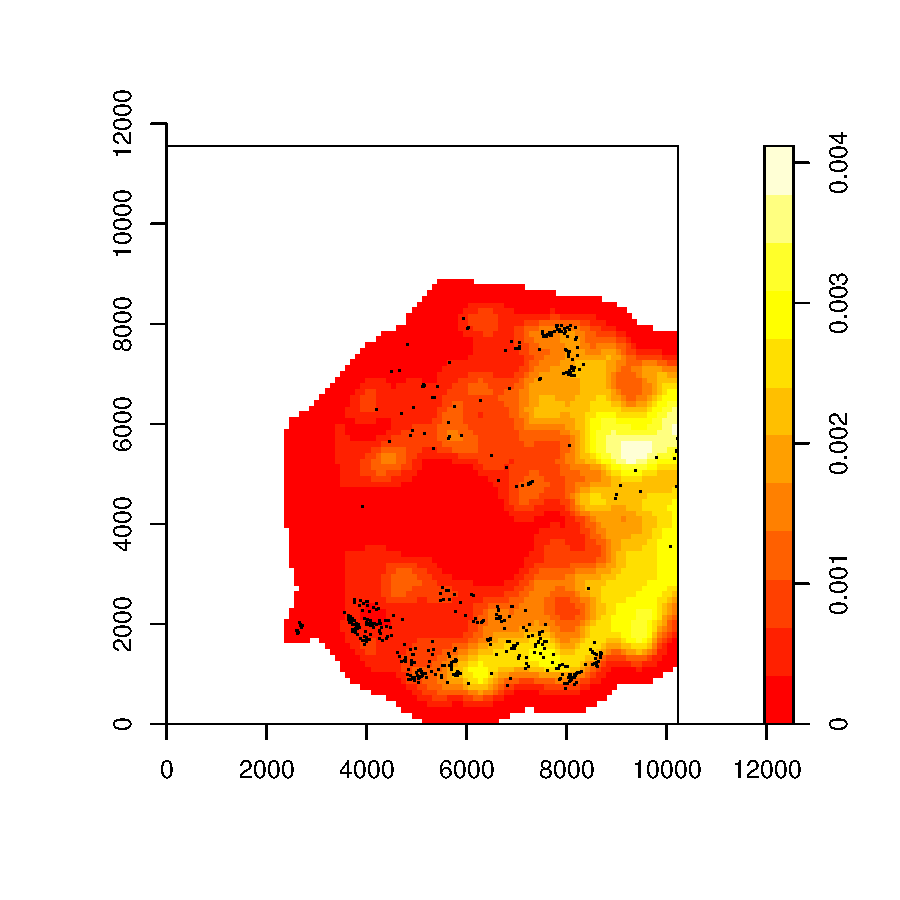
\includegraphics[scale=.5]{Fig2healthyDC.pdf}
  \end{figure}
\end{frame}

\begin{frame}{Breast Cancer Data: Survival}
  \begin{figure}
    \centering
    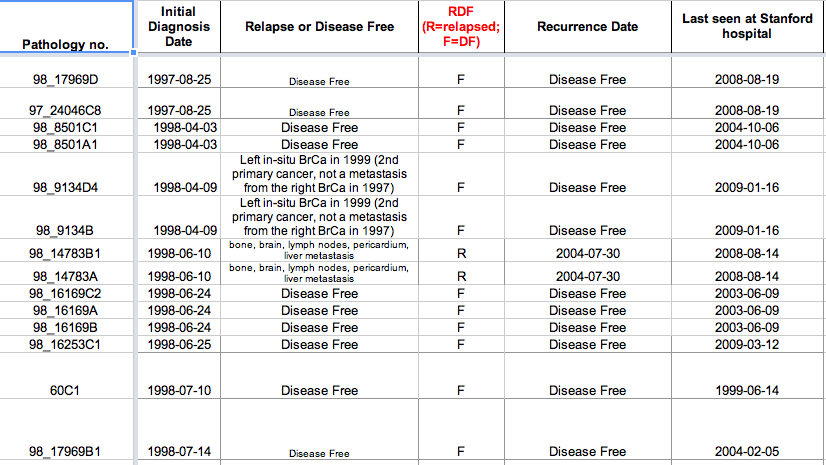
\includegraphics[scale=.5]{survival.png}
  \end{figure}
\end{frame}

\begin{frame}{Breast Cancer Data: Medical}
  \begin{figure}
    \centering
    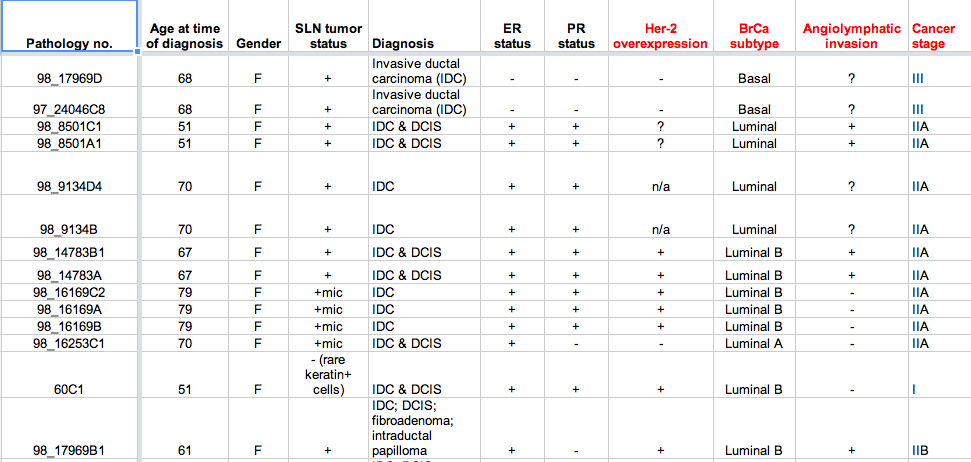
\includegraphics[scale=.5]{medical.png}
  \end{figure}
\end{frame}

\begin{frame}{Breast Cancer Study Questions}
  \begin{itemize}
  \item How do you deal with the data integration problem? \pause
  \item kernel methods via Friedman's procedure \pause
  \item Are there any differences (spatial, medical) between women who
    relapse and those who remain disease free? \pause
  \item two-sample tests
  \end{itemize}
\end{frame}

\begin{frame}{Friedman's Two-Sample Test}
  Friedman (2003) \\
  $\{\mathbf{x}_i\}_{i=1}^N$ from $p(\mathbf{x})$ and
  $\{\mathbf{x}_i\}_{i=N+1}^{N+M}$ from $q(\mathbf{x})$ testing \\
  $\mathcal{H}_A$: $p \neq q$ against $\mathcal{H}_0$: $p = q$ \pause
  \begin{enumerate}
  \item Label the first group $y_i = 1$ and the second group $y_i = -1$ . \pause
  \item Score the observations $\{s_i := f(\mathbf{x}_i)\}_1^{N+M}$ with a learning machine $f$. \pause
  \item Calculate a univariate two-sample test statistic
    $T = T(\{s_i\}_1^N,\{s_i\}_{N+1}^{N+M})$. \pause
  \item Conduct statistical inference based on the permutation null distribution of the above
    statistic.
  \end{enumerate}
\end{frame}

\begin{frame}{Twitter Example}
  \begin{figure}[!ht]
   \centering
   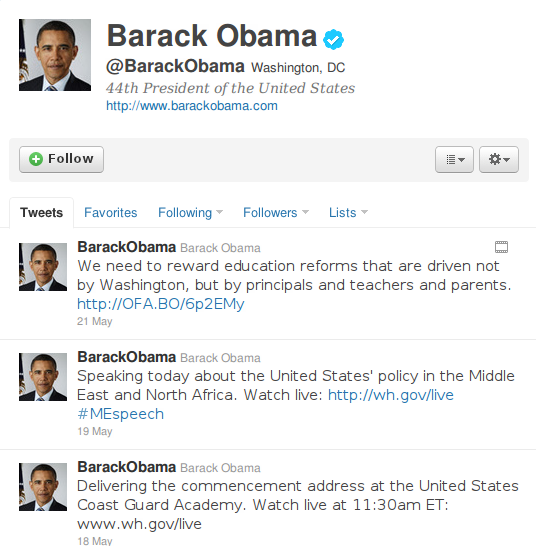
\includegraphics[scale=.3]{pres3.png}
   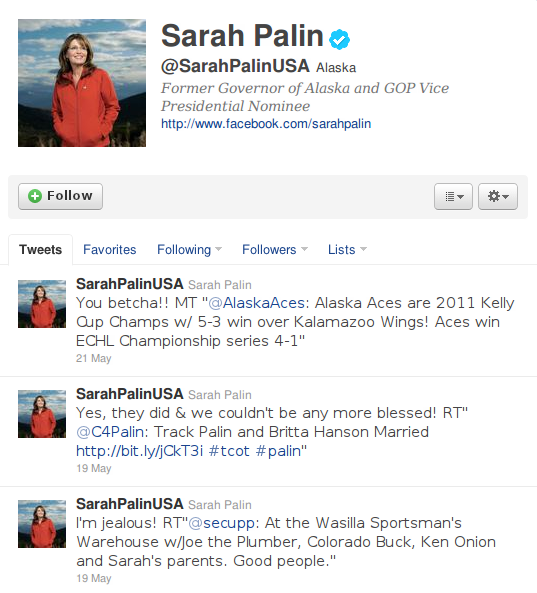
\includegraphics[scale=.3]{pres4.png}
 \end{figure}
\end{frame}

\begin{frame}[fragile]{Non-vectorial Data}
\begin{verbatim}
"BarackObama: We need to reward education reforms that are
driven not by Washington, but by principals and teachers and
parents. http://OFA.BO/6p2EMy"
\end{verbatim}
\pause

$\bar{x} = $ ? \\ \pause
$\hat{\sigma}_x = $ ? \\ \pause
Kernel methods allow us to lift ourselves up into an inner product space, where we can perform geometric calculations.
\end{frame}

\section{Kernel-based Tests}
\begin{frame}{Kernel Methods}
  The Kernel Trick (Aizerman et al. 1964) \pause
  \begin{itemize}
  \item Data $x_i$ in a general set $\mathcal{X}$. \pause
  \item Define a feature map $\phi : \mathcal{X} \to V$, where $V$ is an inner product space. \pause
  \item $K(u_i, u_j) = \langle \phi(u_i), \phi(u_j) \rangle$ \pause
  \item Use learning algorithms that only require inner products between vectors in $\mathcal{X}$. \pause
  \item The inner products can be done implicitly, by a kernel function $K: \mathcal{X} \times \mathcal{X} \to \mathbb{R}$.
  \end{itemize}
\end{frame}

\begin{frame}[fragile]{Twitter Data}
  Raw:
\begin{verbatim}
"BarackObama: We need to reward education reforms that are
driven not by Washington, but by principals and teachers and
parents. http://OFA.BO/6p2EMy"
"SarahPalinUSA: You betcha!! MT \"@AlaskaAces: Alaska Aces
are 2011 Kelly Cup Champs w/ 5-3 win over Kalamazoo Wings!
Aces win  ECHL Championship series 4-1\""
\end{verbatim}
  After pre-processing:
\begin{verbatim}
"we need to reward education reforms that are driven not by
washington but by principals and teachers and parents "
"you betcha mt alaskaaces alaska aces are  kelly cup champs
w  win over kalamazoo wings aces win  echl championship
series "
\end{verbatim}
\end{frame}

\begin{frame}{The Spectrum Kernel}
  The Spectrum Kernel (Leslie 2002) \\ \pause
  Compares two strings based on the their length $k$ contiguous
  subsequences ($k$-mers). \pause
  \begin{itemize}
    \item $\mathcal{X} = $ set of all finite-length sequences from an alphabet $\mathcal{A}$. \pause
    \item $\phi_2(x) = [\#_{\text{aa}}(x), \#_{\text{ab}}(x), \#_{\text{ac}}(x), \ldots ]$ \pause
    \item $\mathcal{V} = \mathbb{N}^{|\mathcal{A}|^k}$ \pause
    \item $K_k(x,y) = \langle \phi_k(x), \phi_k(y) \rangle$
  \end{itemize}
\end{frame}

\begin{frame}{Support Vector Machines}
$\ell_1$-regularized (soft-margin) support vector classification problem
(Vapnik and Cortes, 1995): \pause
\begin{equation*}
\begin{aligned}
& \underset{\mathbf{w} \in \mathcal{H}, b \in \mathbb{R}}{\text{minimize}}
& &\frac{1}{2}\norm{\mathbf{w}}^2+C\sum_{i=1}^M \xi_i \\
& \text{subject to}
& & y_i(\mathbf{w}^t \mathbf{x}_i + b) \geq 1 - \xi_i \\
&&& \xi_i \geq 0 \qquad \qquad \quad \text{for all } i=1,\ldots,m. \pause
\end{aligned}
\end{equation*}
For the Friedman Test, our scoring function is the margin
$f(\mathbf{x}_i) = \sum_{i=1}^m y_i \alpha_i K(\mathbf{x}, \mathbf{x}_i) + b$.
\end{frame}

\begin{frame}{KMMD}
  Kernel Maximum Mean Discrepancy Test: (Gretton et al. 2006) \\ \pause
  $\mathfrak{F}$ a class of functions (unit ball in RKHS), $f:\mathcal{X} \to \mathbb{R}$,
  $p$ and $q$ probability distributions, and $X \sim p$ and $Z \sim q$ random variables \\ \pause

  MMD statistic:
  \begin{equation*}
    \text{MMD}[\mathfrak{F},p,q] := \sup_{f\in
      \mathfrak{F}}(\mathbb{E}_{x\sim p}[f(x)] - \mathbb{E}_{z\sim q}[f(z)]) \pause
  \end{equation*}

  Empirical Estimate:
  \begin{equation*}
    \text{MMD}[\mathfrak{F},X,Z] := \sup_{f\in
      \mathfrak{F}}\left (\frac{1}{N}\sum_{i=1}^Nf(x_i) -
    \frac{1}{M}\sum_{i=1}^M f(z_i) \right )
  \end{equation*}
\end{frame}

\begin{frame}{Twitter Example}
  \begin{center}
    \resizebox{10.0cm}{!}{
      % Created by tikzDevice version 0.6.2-92-0ad2792 on 2013-03-31 12:28:06
% !TEX encoding = UTF-8 Unicode
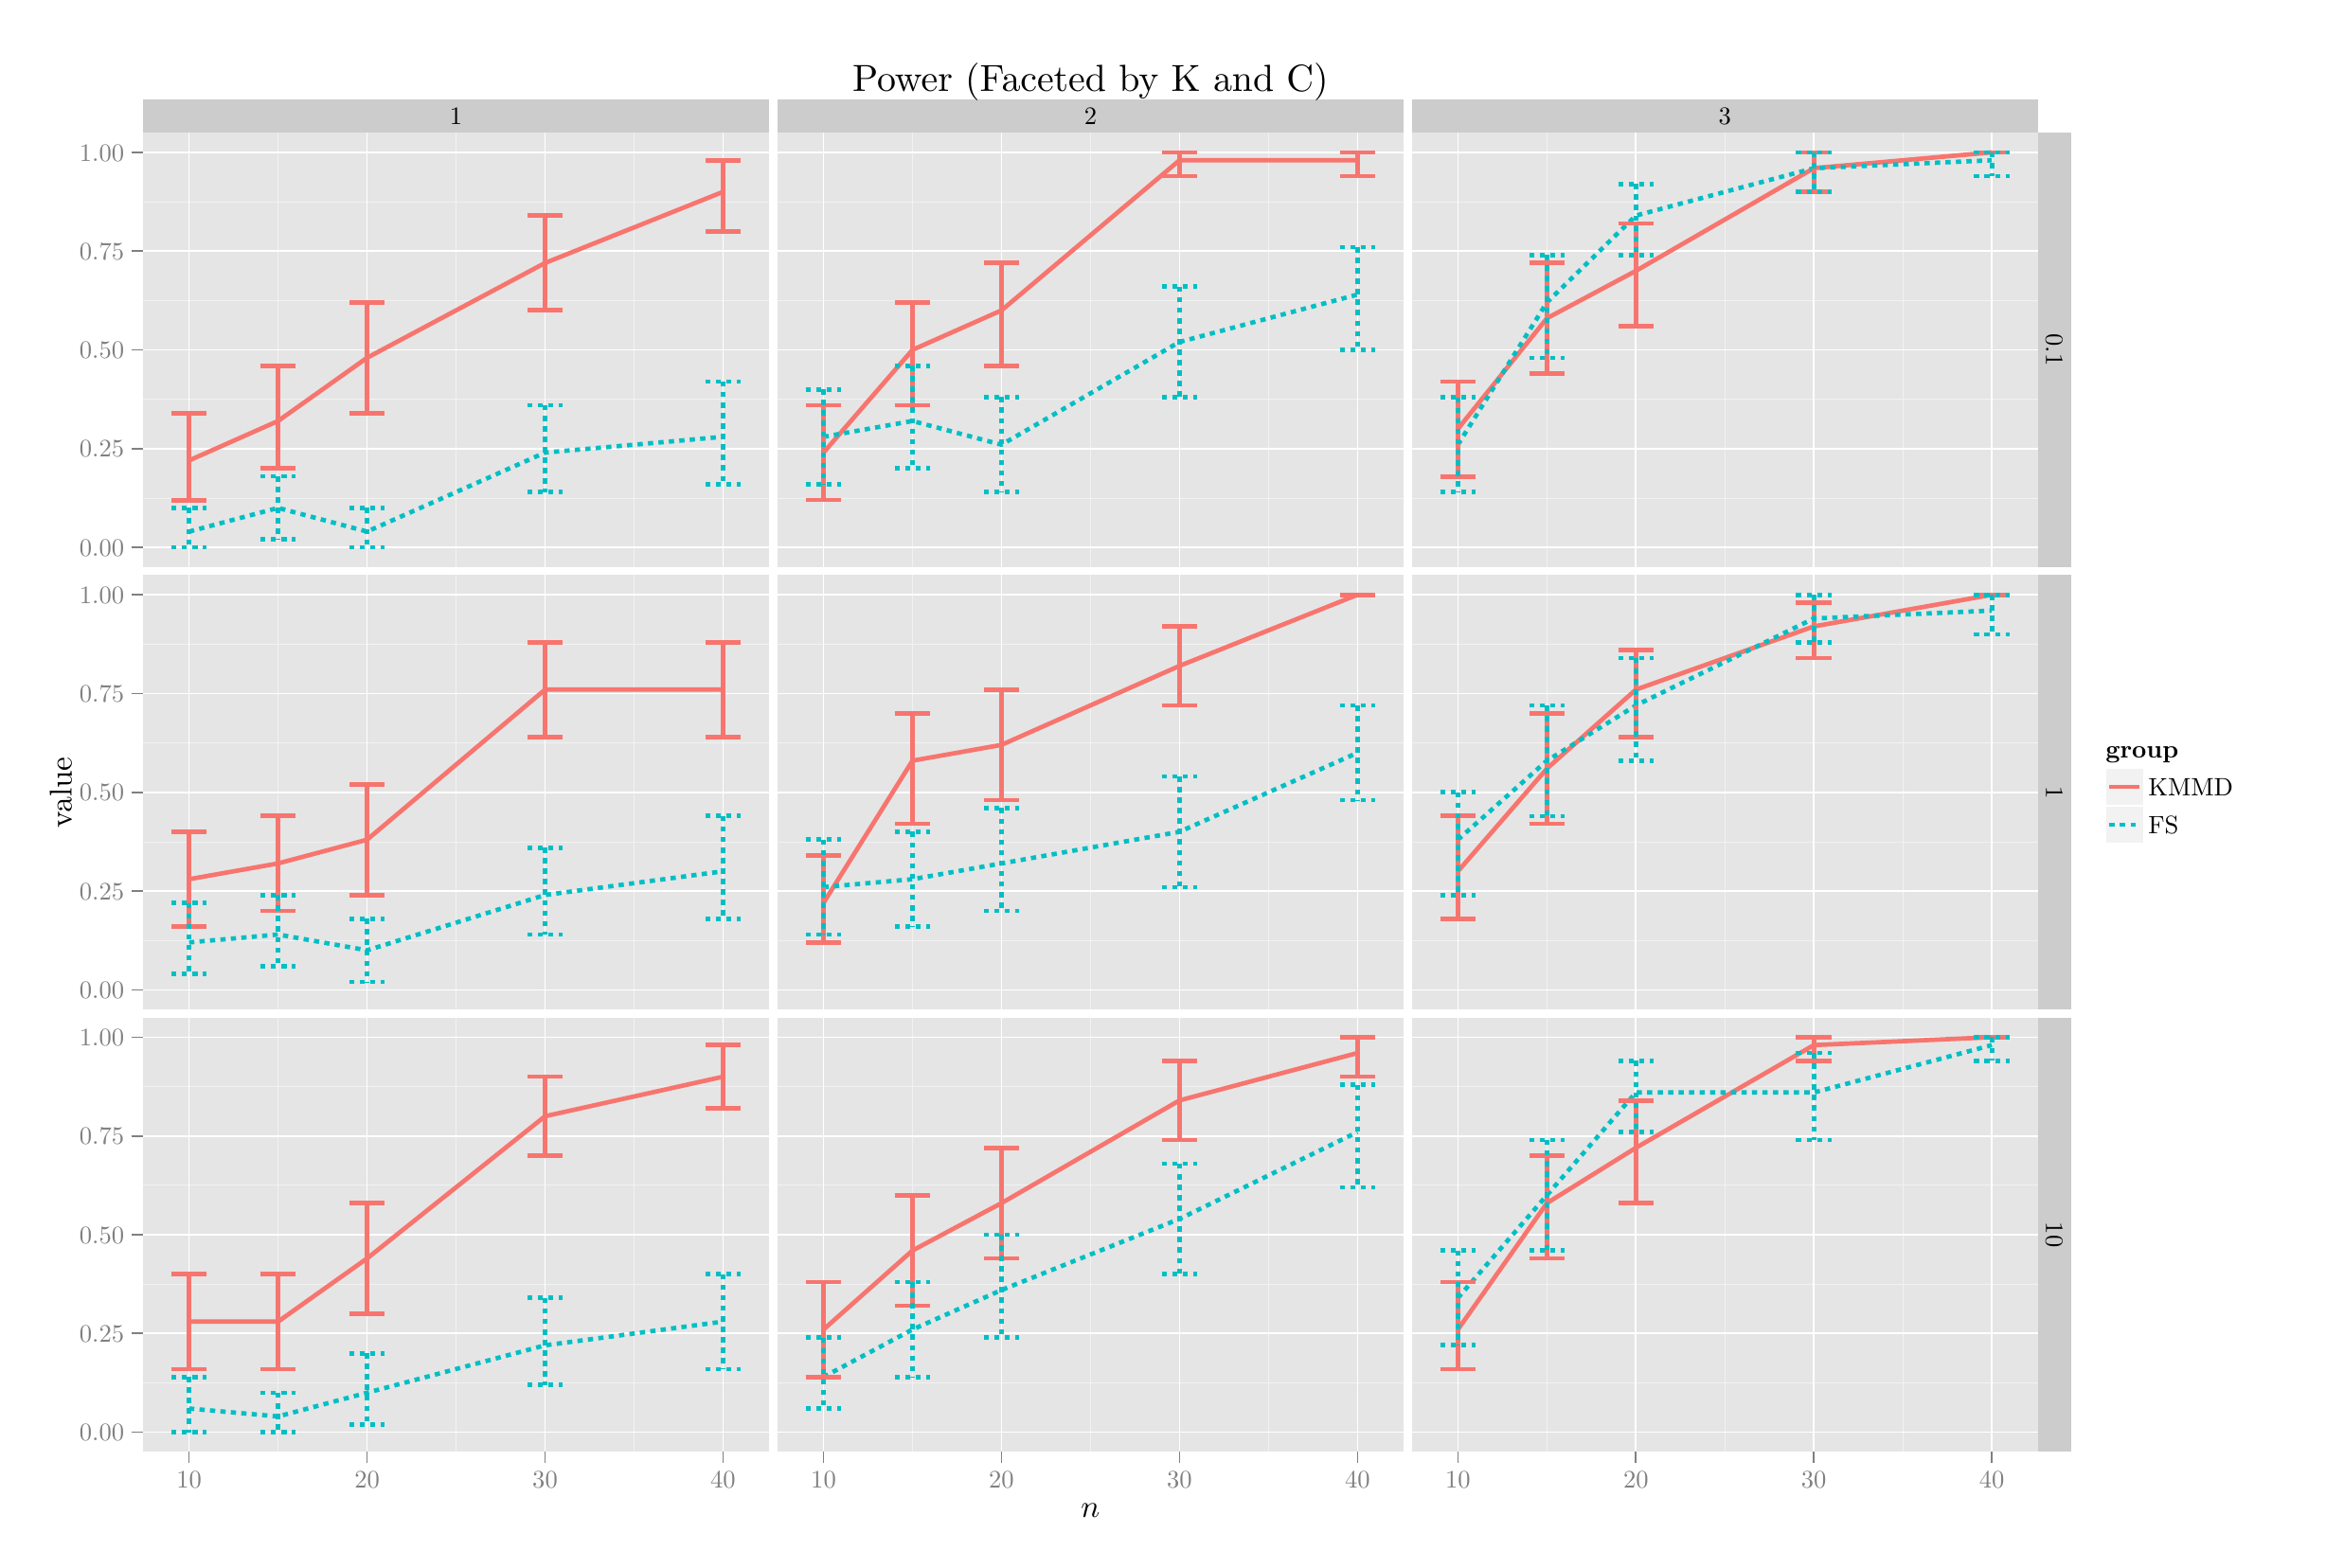
\begin{tikzpicture}[x=1pt,y=1pt]
\definecolor[named]{fillColor}{rgb}{1.00,1.00,1.00}
\path[use as bounding box,fill=fillColor,fill opacity=0.00] (0,0) rectangle (867.24,578.16);
\begin{scope}
\path[clip] (  0.00,  0.00) rectangle (867.24,578.16);
\definecolor[named]{drawColor}{rgb}{1.00,1.00,1.00}
\definecolor[named]{fillColor}{rgb}{1.00,1.00,1.00}

\path[draw=drawColor,line width= 0.6pt,line join=round,line cap=round,fill=fillColor] (  0.00, -0.00) rectangle (867.24,578.16);
\end{scope}
\begin{scope}
\path[clip] ( 44.49,537.54) rectangle (283.53,550.17);
\definecolor[named]{fillColor}{rgb}{0.80,0.80,0.80}

\path[fill=fillColor] ( 44.49,537.54) rectangle (283.53,550.17);
\definecolor[named]{drawColor}{rgb}{0.00,0.00,0.00}

\node[text=drawColor,anchor=base,inner sep=0pt, outer sep=0pt, scale=  0.96] at (164.01,540.55) {1};
\end{scope}
\begin{scope}
\path[clip] (286.54,537.54) rectangle (525.58,550.17);
\definecolor[named]{fillColor}{rgb}{0.80,0.80,0.80}

\path[fill=fillColor] (286.54,537.54) rectangle (525.58,550.17);
\definecolor[named]{drawColor}{rgb}{0.00,0.00,0.00}

\node[text=drawColor,anchor=base,inner sep=0pt, outer sep=0pt, scale=  0.96] at (406.06,540.55) {2};
\end{scope}
\begin{scope}
\path[clip] (528.59,537.54) rectangle (767.64,550.17);
\definecolor[named]{fillColor}{rgb}{0.80,0.80,0.80}

\path[fill=fillColor] (528.59,537.54) rectangle (767.64,550.17);
\definecolor[named]{drawColor}{rgb}{0.00,0.00,0.00}

\node[text=drawColor,anchor=base,inner sep=0pt, outer sep=0pt, scale=  0.96] at (648.11,540.55) {3};
\end{scope}
\begin{scope}
\path[clip] ( 44.49,371.71) rectangle (283.53,537.54);
\definecolor[named]{fillColor}{rgb}{0.90,0.90,0.90}

\path[fill=fillColor] ( 44.49,371.71) rectangle (283.53,537.54);
\definecolor[named]{drawColor}{rgb}{0.95,0.95,0.95}

\path[draw=drawColor,line width= 0.3pt,line join=round] ( 44.49,398.09) --
	(283.53,398.09);

\path[draw=drawColor,line width= 0.3pt,line join=round] ( 44.49,435.78) --
	(283.53,435.78);

\path[draw=drawColor,line width= 0.3pt,line join=round] ( 44.49,473.47) --
	(283.53,473.47);

\path[draw=drawColor,line width= 0.3pt,line join=round] ( 44.49,511.16) --
	(283.53,511.16);

\path[draw=drawColor,line width= 0.3pt,line join=round] ( 96.10,371.71) --
	( 96.10,537.54);

\path[draw=drawColor,line width= 0.3pt,line join=round] (164.01,371.71) --
	(164.01,537.54);

\path[draw=drawColor,line width= 0.3pt,line join=round] (231.92,371.71) --
	(231.92,537.54);
\definecolor[named]{drawColor}{rgb}{1.00,1.00,1.00}

\path[draw=drawColor,line width= 0.6pt,line join=round] ( 44.49,379.25) --
	(283.53,379.25);

\path[draw=drawColor,line width= 0.6pt,line join=round] ( 44.49,416.94) --
	(283.53,416.94);

\path[draw=drawColor,line width= 0.6pt,line join=round] ( 44.49,454.63) --
	(283.53,454.63);

\path[draw=drawColor,line width= 0.6pt,line join=round] ( 44.49,492.31) --
	(283.53,492.31);

\path[draw=drawColor,line width= 0.6pt,line join=round] ( 44.49,530.00) --
	(283.53,530.00);

\path[draw=drawColor,line width= 0.6pt,line join=round] ( 62.14,371.71) --
	( 62.14,537.54);

\path[draw=drawColor,line width= 0.6pt,line join=round] (130.05,371.71) --
	(130.05,537.54);

\path[draw=drawColor,line width= 0.6pt,line join=round] (197.96,371.71) --
	(197.96,537.54);

\path[draw=drawColor,line width= 0.6pt,line join=round] (265.87,371.71) --
	(265.87,537.54);
\definecolor[named]{drawColor}{rgb}{0.97,0.46,0.43}

\path[draw=drawColor,line width= 1.7pt,line join=round] ( 62.14,412.42) --
	( 96.10,427.49) --
	(130.05,451.61) --
	(197.96,487.79) --
	(265.87,514.93);
\definecolor[named]{drawColor}{rgb}{0.00,0.75,0.77}

\path[draw=drawColor,line width= 1.7pt,dash pattern=on 2pt off 2pt ,line join=round] ( 62.14,385.28) --
	( 96.10,394.33) --
	(130.05,385.28) --
	(197.96,415.43) --
	(265.87,421.46);
\definecolor[named]{drawColor}{rgb}{0.97,0.46,0.43}

\path[draw=drawColor,line width= 1.7pt,line join=round] ( 55.35,430.51) --
	( 68.93,430.51);

\path[draw=drawColor,line width= 1.7pt,line join=round] ( 62.14,430.51) --
	( 62.14,397.27);

\path[draw=drawColor,line width= 1.7pt,line join=round] ( 55.35,397.27) --
	( 68.93,397.27);

\path[draw=drawColor,line width= 1.7pt,line join=round] ( 89.31,448.60) --
	(102.89,448.60);

\path[draw=drawColor,line width= 1.7pt,line join=round] ( 96.10,448.60) --
	( 96.10,409.40);

\path[draw=drawColor,line width= 1.7pt,line join=round] ( 89.31,409.40) --
	(102.89,409.40);

\path[draw=drawColor,line width= 1.7pt,line join=round] (123.26,472.72) --
	(136.84,472.72);

\path[draw=drawColor,line width= 1.7pt,line join=round] (130.05,472.72) --
	(130.05,430.51);

\path[draw=drawColor,line width= 1.7pt,line join=round] (123.26,430.51) --
	(136.84,430.51);

\path[draw=drawColor,line width= 1.7pt,line join=round] (191.17,505.88) --
	(204.75,505.88);

\path[draw=drawColor,line width= 1.7pt,line join=round] (197.96,505.88) --
	(197.96,469.70);

\path[draw=drawColor,line width= 1.7pt,line join=round] (191.17,469.70) --
	(204.75,469.70);

\path[draw=drawColor,line width= 1.7pt,line join=round] (259.08,526.99) --
	(272.66,526.99);

\path[draw=drawColor,line width= 1.7pt,line join=round] (265.87,526.99) --
	(265.87,499.85);

\path[draw=drawColor,line width= 1.7pt,line join=round] (259.08,499.85) --
	(272.66,499.85);
\definecolor[named]{drawColor}{rgb}{0.00,0.75,0.77}

\path[draw=drawColor,line width= 1.7pt,dash pattern=on 2pt off 2pt ,line join=round] ( 55.35,394.33) --
	( 68.93,394.33);

\path[draw=drawColor,line width= 1.7pt,dash pattern=on 2pt off 2pt ,line join=round] ( 62.14,394.33) --
	( 62.14,379.25);

\path[draw=drawColor,line width= 1.7pt,dash pattern=on 2pt off 2pt ,line join=round] ( 55.35,379.25) --
	( 68.93,379.25);

\path[draw=drawColor,line width= 1.7pt,dash pattern=on 2pt off 2pt ,line join=round] ( 89.31,406.39) --
	(102.89,406.39);

\path[draw=drawColor,line width= 1.7pt,dash pattern=on 2pt off 2pt ,line join=round] ( 96.10,406.39) --
	( 96.10,382.27);

\path[draw=drawColor,line width= 1.7pt,dash pattern=on 2pt off 2pt ,line join=round] ( 89.31,382.27) --
	(102.89,382.27);

\path[draw=drawColor,line width= 1.7pt,dash pattern=on 2pt off 2pt ,line join=round] (123.26,394.33) --
	(136.84,394.33);

\path[draw=drawColor,line width= 1.7pt,dash pattern=on 2pt off 2pt ,line join=round] (130.05,394.33) --
	(130.05,379.25);

\path[draw=drawColor,line width= 1.7pt,dash pattern=on 2pt off 2pt ,line join=round] (123.26,379.25) --
	(136.84,379.25);

\path[draw=drawColor,line width= 1.7pt,dash pattern=on 2pt off 2pt ,line join=round] (191.17,433.52) --
	(204.75,433.52);

\path[draw=drawColor,line width= 1.7pt,dash pattern=on 2pt off 2pt ,line join=round] (197.96,433.52) --
	(197.96,400.36);

\path[draw=drawColor,line width= 1.7pt,dash pattern=on 2pt off 2pt ,line join=round] (191.17,400.36) --
	(204.75,400.36);

\path[draw=drawColor,line width= 1.7pt,dash pattern=on 2pt off 2pt ,line join=round] (259.08,442.57) --
	(272.66,442.57);

\path[draw=drawColor,line width= 1.7pt,dash pattern=on 2pt off 2pt ,line join=round] (265.87,442.57) --
	(265.87,403.37);

\path[draw=drawColor,line width= 1.7pt,dash pattern=on 2pt off 2pt ,line join=round] (259.08,403.37) --
	(272.66,403.37);
\end{scope}
\begin{scope}
\path[clip] ( 44.49,202.87) rectangle (283.53,368.70);
\definecolor[named]{fillColor}{rgb}{0.90,0.90,0.90}

\path[fill=fillColor] ( 44.49,202.87) rectangle (283.53,368.70);
\definecolor[named]{drawColor}{rgb}{0.95,0.95,0.95}

\path[draw=drawColor,line width= 0.3pt,line join=round] ( 44.49,229.26) --
	(283.53,229.26);

\path[draw=drawColor,line width= 0.3pt,line join=round] ( 44.49,266.94) --
	(283.53,266.94);

\path[draw=drawColor,line width= 0.3pt,line join=round] ( 44.49,304.63) --
	(283.53,304.63);

\path[draw=drawColor,line width= 0.3pt,line join=round] ( 44.49,342.32) --
	(283.53,342.32);

\path[draw=drawColor,line width= 0.3pt,line join=round] ( 96.10,202.87) --
	( 96.10,368.70);

\path[draw=drawColor,line width= 0.3pt,line join=round] (164.01,202.87) --
	(164.01,368.70);

\path[draw=drawColor,line width= 0.3pt,line join=round] (231.92,202.87) --
	(231.92,368.70);
\definecolor[named]{drawColor}{rgb}{1.00,1.00,1.00}

\path[draw=drawColor,line width= 0.6pt,line join=round] ( 44.49,210.41) --
	(283.53,210.41);

\path[draw=drawColor,line width= 0.6pt,line join=round] ( 44.49,248.10) --
	(283.53,248.10);

\path[draw=drawColor,line width= 0.6pt,line join=round] ( 44.49,285.79) --
	(283.53,285.79);

\path[draw=drawColor,line width= 0.6pt,line join=round] ( 44.49,323.48) --
	(283.53,323.48);

\path[draw=drawColor,line width= 0.6pt,line join=round] ( 44.49,361.16) --
	(283.53,361.16);

\path[draw=drawColor,line width= 0.6pt,line join=round] ( 62.14,202.87) --
	( 62.14,368.70);

\path[draw=drawColor,line width= 0.6pt,line join=round] (130.05,202.87) --
	(130.05,368.70);

\path[draw=drawColor,line width= 0.6pt,line join=round] (197.96,202.87) --
	(197.96,368.70);

\path[draw=drawColor,line width= 0.6pt,line join=round] (265.87,202.87) --
	(265.87,368.70);
\definecolor[named]{drawColor}{rgb}{0.97,0.46,0.43}

\path[draw=drawColor,line width= 1.7pt,line join=round] ( 62.14,252.62) --
	( 96.10,258.65) --
	(130.05,267.70) --
	(197.96,324.98) --
	(265.87,324.98);
\definecolor[named]{drawColor}{rgb}{0.00,0.75,0.77}

\path[draw=drawColor,line width= 1.7pt,dash pattern=on 2pt off 2pt ,line join=round] ( 62.14,228.50) --
	( 96.10,231.52) --
	(130.05,225.49) --
	(197.96,246.59) --
	(265.87,255.64);
\definecolor[named]{drawColor}{rgb}{0.97,0.46,0.43}

\path[draw=drawColor,line width= 1.7pt,line join=round] ( 55.35,270.71) --
	( 68.93,270.71);

\path[draw=drawColor,line width= 1.7pt,line join=round] ( 62.14,270.71) --
	( 62.14,234.53);

\path[draw=drawColor,line width= 1.7pt,line join=round] ( 55.35,234.53) --
	( 68.93,234.53);

\path[draw=drawColor,line width= 1.7pt,line join=round] ( 89.31,276.74) --
	(102.89,276.74);

\path[draw=drawColor,line width= 1.7pt,line join=round] ( 96.10,276.74) --
	( 96.10,240.56);

\path[draw=drawColor,line width= 1.7pt,line join=round] ( 89.31,240.56) --
	(102.89,240.56);

\path[draw=drawColor,line width= 1.7pt,line join=round] (123.26,288.80) --
	(136.84,288.80);

\path[draw=drawColor,line width= 1.7pt,line join=round] (130.05,288.80) --
	(130.05,246.59);

\path[draw=drawColor,line width= 1.7pt,line join=round] (123.26,246.59) --
	(136.84,246.59);

\path[draw=drawColor,line width= 1.7pt,line join=round] (191.17,343.07) --
	(204.75,343.07);

\path[draw=drawColor,line width= 1.7pt,line join=round] (197.96,343.07) --
	(197.96,306.89);

\path[draw=drawColor,line width= 1.7pt,line join=round] (191.17,306.89) --
	(204.75,306.89);

\path[draw=drawColor,line width= 1.7pt,line join=round] (259.08,343.07) --
	(272.66,343.07);

\path[draw=drawColor,line width= 1.7pt,line join=round] (265.87,343.07) --
	(265.87,306.89);

\path[draw=drawColor,line width= 1.7pt,line join=round] (259.08,306.89) --
	(272.66,306.89);
\definecolor[named]{drawColor}{rgb}{0.00,0.75,0.77}

\path[draw=drawColor,line width= 1.7pt,dash pattern=on 2pt off 2pt ,line join=round] ( 55.35,243.58) --
	( 68.93,243.58);

\path[draw=drawColor,line width= 1.7pt,dash pattern=on 2pt off 2pt ,line join=round] ( 62.14,243.58) --
	( 62.14,216.44);

\path[draw=drawColor,line width= 1.7pt,dash pattern=on 2pt off 2pt ,line join=round] ( 55.35,216.44) --
	( 68.93,216.44);

\path[draw=drawColor,line width= 1.7pt,dash pattern=on 2pt off 2pt ,line join=round] ( 89.31,246.59) --
	(102.89,246.59);

\path[draw=drawColor,line width= 1.7pt,dash pattern=on 2pt off 2pt ,line join=round] ( 96.10,246.59) --
	( 96.10,219.46);

\path[draw=drawColor,line width= 1.7pt,dash pattern=on 2pt off 2pt ,line join=round] ( 89.31,219.46) --
	(102.89,219.46);

\path[draw=drawColor,line width= 1.7pt,dash pattern=on 2pt off 2pt ,line join=round] (123.26,237.55) --
	(136.84,237.55);

\path[draw=drawColor,line width= 1.7pt,dash pattern=on 2pt off 2pt ,line join=round] (130.05,237.55) --
	(130.05,213.43);

\path[draw=drawColor,line width= 1.7pt,dash pattern=on 2pt off 2pt ,line join=round] (123.26,213.43) --
	(136.84,213.43);

\path[draw=drawColor,line width= 1.7pt,dash pattern=on 2pt off 2pt ,line join=round] (191.17,264.68) --
	(204.75,264.68);

\path[draw=drawColor,line width= 1.7pt,dash pattern=on 2pt off 2pt ,line join=round] (197.96,264.68) --
	(197.96,231.52);

\path[draw=drawColor,line width= 1.7pt,dash pattern=on 2pt off 2pt ,line join=round] (191.17,231.52) --
	(204.75,231.52);

\path[draw=drawColor,line width= 1.7pt,dash pattern=on 2pt off 2pt ,line join=round] (259.08,276.74) --
	(272.66,276.74);

\path[draw=drawColor,line width= 1.7pt,dash pattern=on 2pt off 2pt ,line join=round] (265.87,276.74) --
	(265.87,237.55);

\path[draw=drawColor,line width= 1.7pt,dash pattern=on 2pt off 2pt ,line join=round] (259.08,237.55) --
	(272.66,237.55);
\end{scope}
\begin{scope}
\path[clip] ( 44.49, 34.03) rectangle (283.53,199.86);
\definecolor[named]{fillColor}{rgb}{0.90,0.90,0.90}

\path[fill=fillColor] ( 44.49, 34.03) rectangle (283.53,199.86);
\definecolor[named]{drawColor}{rgb}{0.95,0.95,0.95}

\path[draw=drawColor,line width= 0.3pt,line join=round] ( 44.49, 60.42) --
	(283.53, 60.42);

\path[draw=drawColor,line width= 0.3pt,line join=round] ( 44.49, 98.10) --
	(283.53, 98.10);

\path[draw=drawColor,line width= 0.3pt,line join=round] ( 44.49,135.79) --
	(283.53,135.79);

\path[draw=drawColor,line width= 0.3pt,line join=round] ( 44.49,173.48) --
	(283.53,173.48);

\path[draw=drawColor,line width= 0.3pt,line join=round] ( 96.10, 34.03) --
	( 96.10,199.86);

\path[draw=drawColor,line width= 0.3pt,line join=round] (164.01, 34.03) --
	(164.01,199.86);

\path[draw=drawColor,line width= 0.3pt,line join=round] (231.92, 34.03) --
	(231.92,199.86);
\definecolor[named]{drawColor}{rgb}{1.00,1.00,1.00}

\path[draw=drawColor,line width= 0.6pt,line join=round] ( 44.49, 41.57) --
	(283.53, 41.57);

\path[draw=drawColor,line width= 0.6pt,line join=round] ( 44.49, 79.26) --
	(283.53, 79.26);

\path[draw=drawColor,line width= 0.6pt,line join=round] ( 44.49,116.95) --
	(283.53,116.95);

\path[draw=drawColor,line width= 0.6pt,line join=round] ( 44.49,154.64) --
	(283.53,154.64);

\path[draw=drawColor,line width= 0.6pt,line join=round] ( 44.49,192.32) --
	(283.53,192.32);

\path[draw=drawColor,line width= 0.6pt,line join=round] ( 62.14, 34.03) --
	( 62.14,199.86);

\path[draw=drawColor,line width= 0.6pt,line join=round] (130.05, 34.03) --
	(130.05,199.86);

\path[draw=drawColor,line width= 0.6pt,line join=round] (197.96, 34.03) --
	(197.96,199.86);

\path[draw=drawColor,line width= 0.6pt,line join=round] (265.87, 34.03) --
	(265.87,199.86);
\definecolor[named]{drawColor}{rgb}{0.97,0.46,0.43}

\path[draw=drawColor,line width= 1.7pt,line join=round] ( 62.14, 83.78) --
	( 96.10, 83.78) --
	(130.05,107.90) --
	(197.96,162.17) --
	(265.87,177.25);
\definecolor[named]{drawColor}{rgb}{0.00,0.75,0.77}

\path[draw=drawColor,line width= 1.7pt,dash pattern=on 2pt off 2pt ,line join=round] ( 62.14, 50.62) --
	( 96.10, 47.60) --
	(130.05, 56.65) --
	(197.96, 74.74) --
	(265.87, 83.78);
\definecolor[named]{drawColor}{rgb}{0.97,0.46,0.43}

\path[draw=drawColor,line width= 1.7pt,line join=round] ( 55.35,101.87) --
	( 68.93,101.87);

\path[draw=drawColor,line width= 1.7pt,line join=round] ( 62.14,101.87) --
	( 62.14, 65.69);

\path[draw=drawColor,line width= 1.7pt,line join=round] ( 55.35, 65.69) --
	( 68.93, 65.69);

\path[draw=drawColor,line width= 1.7pt,line join=round] ( 89.31,101.87) --
	(102.89,101.87);

\path[draw=drawColor,line width= 1.7pt,line join=round] ( 96.10,101.87) --
	( 96.10, 65.69);

\path[draw=drawColor,line width= 1.7pt,line join=round] ( 89.31, 65.69) --
	(102.89, 65.69);

\path[draw=drawColor,line width= 1.7pt,line join=round] (123.26,129.01) --
	(136.84,129.01);

\path[draw=drawColor,line width= 1.7pt,line join=round] (130.05,129.01) --
	(130.05, 86.80);

\path[draw=drawColor,line width= 1.7pt,line join=round] (123.26, 86.80) --
	(136.84, 86.80);

\path[draw=drawColor,line width= 1.7pt,line join=round] (191.17,177.25) --
	(204.75,177.25);

\path[draw=drawColor,line width= 1.7pt,line join=round] (197.96,177.25) --
	(197.96,147.10);

\path[draw=drawColor,line width= 1.7pt,line join=round] (191.17,147.10) --
	(204.75,147.10);

\path[draw=drawColor,line width= 1.7pt,line join=round] (259.08,189.31) --
	(272.66,189.31);

\path[draw=drawColor,line width= 1.7pt,line join=round] (265.87,189.31) --
	(265.87,165.19);

\path[draw=drawColor,line width= 1.7pt,line join=round] (259.08,165.19) --
	(272.66,165.19);
\definecolor[named]{drawColor}{rgb}{0.00,0.75,0.77}

\path[draw=drawColor,line width= 1.7pt,dash pattern=on 2pt off 2pt ,line join=round] ( 55.35, 62.68) --
	( 68.93, 62.68);

\path[draw=drawColor,line width= 1.7pt,dash pattern=on 2pt off 2pt ,line join=round] ( 62.14, 62.68) --
	( 62.14, 41.57);

\path[draw=drawColor,line width= 1.7pt,dash pattern=on 2pt off 2pt ,line join=round] ( 55.35, 41.57) --
	( 68.93, 41.57);

\path[draw=drawColor,line width= 1.7pt,dash pattern=on 2pt off 2pt ,line join=round] ( 89.31, 56.65) --
	(102.89, 56.65);

\path[draw=drawColor,line width= 1.7pt,dash pattern=on 2pt off 2pt ,line join=round] ( 96.10, 56.65) --
	( 96.10, 41.57);

\path[draw=drawColor,line width= 1.7pt,dash pattern=on 2pt off 2pt ,line join=round] ( 89.31, 41.57) --
	(102.89, 41.57);

\path[draw=drawColor,line width= 1.7pt,dash pattern=on 2pt off 2pt ,line join=round] (123.26, 71.72) --
	(136.84, 71.72);

\path[draw=drawColor,line width= 1.7pt,dash pattern=on 2pt off 2pt ,line join=round] (130.05, 71.72) --
	(130.05, 44.59);

\path[draw=drawColor,line width= 1.7pt,dash pattern=on 2pt off 2pt ,line join=round] (123.26, 44.59) --
	(136.84, 44.59);

\path[draw=drawColor,line width= 1.7pt,dash pattern=on 2pt off 2pt ,line join=round] (191.17, 92.83) --
	(204.75, 92.83);

\path[draw=drawColor,line width= 1.7pt,dash pattern=on 2pt off 2pt ,line join=round] (197.96, 92.83) --
	(197.96, 59.66);

\path[draw=drawColor,line width= 1.7pt,dash pattern=on 2pt off 2pt ,line join=round] (191.17, 59.66) --
	(204.75, 59.66);

\path[draw=drawColor,line width= 1.7pt,dash pattern=on 2pt off 2pt ,line join=round] (259.08,101.87) --
	(272.66,101.87);

\path[draw=drawColor,line width= 1.7pt,dash pattern=on 2pt off 2pt ,line join=round] (265.87,101.87) --
	(265.87, 65.69);

\path[draw=drawColor,line width= 1.7pt,dash pattern=on 2pt off 2pt ,line join=round] (259.08, 65.69) --
	(272.66, 65.69);
\end{scope}
\begin{scope}
\path[clip] (286.54,371.71) rectangle (525.58,537.54);
\definecolor[named]{fillColor}{rgb}{0.90,0.90,0.90}

\path[fill=fillColor] (286.54,371.71) rectangle (525.58,537.54);
\definecolor[named]{drawColor}{rgb}{0.95,0.95,0.95}

\path[draw=drawColor,line width= 0.3pt,line join=round] (286.54,398.09) --
	(525.58,398.09);

\path[draw=drawColor,line width= 0.3pt,line join=round] (286.54,435.78) --
	(525.58,435.78);

\path[draw=drawColor,line width= 0.3pt,line join=round] (286.54,473.47) --
	(525.58,473.47);

\path[draw=drawColor,line width= 0.3pt,line join=round] (286.54,511.16) --
	(525.58,511.16);

\path[draw=drawColor,line width= 0.3pt,line join=round] (338.15,371.71) --
	(338.15,537.54);

\path[draw=drawColor,line width= 0.3pt,line join=round] (406.06,371.71) --
	(406.06,537.54);

\path[draw=drawColor,line width= 0.3pt,line join=round] (473.97,371.71) --
	(473.97,537.54);
\definecolor[named]{drawColor}{rgb}{1.00,1.00,1.00}

\path[draw=drawColor,line width= 0.6pt,line join=round] (286.54,379.25) --
	(525.58,379.25);

\path[draw=drawColor,line width= 0.6pt,line join=round] (286.54,416.94) --
	(525.58,416.94);

\path[draw=drawColor,line width= 0.6pt,line join=round] (286.54,454.63) --
	(525.58,454.63);

\path[draw=drawColor,line width= 0.6pt,line join=round] (286.54,492.31) --
	(525.58,492.31);

\path[draw=drawColor,line width= 0.6pt,line join=round] (286.54,530.00) --
	(525.58,530.00);

\path[draw=drawColor,line width= 0.6pt,line join=round] (304.20,371.71) --
	(304.20,537.54);

\path[draw=drawColor,line width= 0.6pt,line join=round] (372.11,371.71) --
	(372.11,537.54);

\path[draw=drawColor,line width= 0.6pt,line join=round] (440.02,371.71) --
	(440.02,537.54);

\path[draw=drawColor,line width= 0.6pt,line join=round] (507.93,371.71) --
	(507.93,537.54);
\definecolor[named]{drawColor}{rgb}{0.97,0.46,0.43}

\path[draw=drawColor,line width= 1.7pt,line join=round] (304.20,415.43) --
	(338.15,454.63) --
	(372.11,469.70) --
	(440.02,526.99) --
	(507.93,526.99);
\definecolor[named]{drawColor}{rgb}{0.00,0.75,0.77}

\path[draw=drawColor,line width= 1.7pt,dash pattern=on 2pt off 2pt ,line join=round] (304.20,421.46) --
	(338.15,427.49) --
	(372.11,418.45) --
	(440.02,457.64) --
	(507.93,475.73);
\definecolor[named]{drawColor}{rgb}{0.97,0.46,0.43}

\path[draw=drawColor,line width= 1.7pt,line join=round] (297.41,433.52) --
	(310.99,433.52);

\path[draw=drawColor,line width= 1.7pt,line join=round] (304.20,433.52) --
	(304.20,397.34);

\path[draw=drawColor,line width= 1.7pt,line join=round] (297.41,397.34) --
	(310.99,397.34);

\path[draw=drawColor,line width= 1.7pt,line join=round] (331.36,472.72) --
	(344.94,472.72);

\path[draw=drawColor,line width= 1.7pt,line join=round] (338.15,472.72) --
	(338.15,433.52);

\path[draw=drawColor,line width= 1.7pt,line join=round] (331.36,433.52) --
	(344.94,433.52);

\path[draw=drawColor,line width= 1.7pt,line join=round] (365.31,487.79) --
	(378.90,487.79);

\path[draw=drawColor,line width= 1.7pt,line join=round] (372.11,487.79) --
	(372.11,448.60);

\path[draw=drawColor,line width= 1.7pt,line join=round] (365.31,448.60) --
	(378.90,448.60);

\path[draw=drawColor,line width= 1.7pt,line join=round] (433.22,530.00) --
	(446.81,530.00);

\path[draw=drawColor,line width= 1.7pt,line join=round] (440.02,530.00) --
	(440.02,520.96);

\path[draw=drawColor,line width= 1.7pt,line join=round] (433.22,520.96) --
	(446.81,520.96);

\path[draw=drawColor,line width= 1.7pt,line join=round] (501.13,530.00) --
	(514.72,530.00);

\path[draw=drawColor,line width= 1.7pt,line join=round] (507.93,530.00) --
	(507.93,520.96);

\path[draw=drawColor,line width= 1.7pt,line join=round] (501.13,520.96) --
	(514.72,520.96);
\definecolor[named]{drawColor}{rgb}{0.00,0.75,0.77}

\path[draw=drawColor,line width= 1.7pt,dash pattern=on 2pt off 2pt ,line join=round] (297.41,439.55) --
	(310.99,439.55);

\path[draw=drawColor,line width= 1.7pt,dash pattern=on 2pt off 2pt ,line join=round] (304.20,439.55) --
	(304.20,403.30);

\path[draw=drawColor,line width= 1.7pt,dash pattern=on 2pt off 2pt ,line join=round] (297.41,403.30) --
	(310.99,403.30);

\path[draw=drawColor,line width= 1.7pt,dash pattern=on 2pt off 2pt ,line join=round] (331.36,448.60) --
	(344.94,448.60);

\path[draw=drawColor,line width= 1.7pt,dash pattern=on 2pt off 2pt ,line join=round] (338.15,448.60) --
	(338.15,409.40);

\path[draw=drawColor,line width= 1.7pt,dash pattern=on 2pt off 2pt ,line join=round] (331.36,409.40) --
	(344.94,409.40);

\path[draw=drawColor,line width= 1.7pt,dash pattern=on 2pt off 2pt ,line join=round] (365.31,436.61) --
	(378.90,436.61);

\path[draw=drawColor,line width= 1.7pt,dash pattern=on 2pt off 2pt ,line join=round] (372.11,436.61) --
	(372.11,400.36);

\path[draw=drawColor,line width= 1.7pt,dash pattern=on 2pt off 2pt ,line join=round] (365.31,400.36) --
	(378.90,400.36);

\path[draw=drawColor,line width= 1.7pt,dash pattern=on 2pt off 2pt ,line join=round] (433.22,478.75) --
	(446.81,478.75);

\path[draw=drawColor,line width= 1.7pt,dash pattern=on 2pt off 2pt ,line join=round] (440.02,478.75) --
	(440.02,436.54);

\path[draw=drawColor,line width= 1.7pt,dash pattern=on 2pt off 2pt ,line join=round] (433.22,436.54) --
	(446.81,436.54);

\path[draw=drawColor,line width= 1.7pt,dash pattern=on 2pt off 2pt ,line join=round] (501.13,493.82) --
	(514.72,493.82);

\path[draw=drawColor,line width= 1.7pt,dash pattern=on 2pt off 2pt ,line join=round] (507.93,493.82) --
	(507.93,454.63);

\path[draw=drawColor,line width= 1.7pt,dash pattern=on 2pt off 2pt ,line join=round] (501.13,454.63) --
	(514.72,454.63);
\end{scope}
\begin{scope}
\path[clip] (286.54,202.87) rectangle (525.58,368.70);
\definecolor[named]{fillColor}{rgb}{0.90,0.90,0.90}

\path[fill=fillColor] (286.54,202.87) rectangle (525.58,368.70);
\definecolor[named]{drawColor}{rgb}{0.95,0.95,0.95}

\path[draw=drawColor,line width= 0.3pt,line join=round] (286.54,229.26) --
	(525.58,229.26);

\path[draw=drawColor,line width= 0.3pt,line join=round] (286.54,266.94) --
	(525.58,266.94);

\path[draw=drawColor,line width= 0.3pt,line join=round] (286.54,304.63) --
	(525.58,304.63);

\path[draw=drawColor,line width= 0.3pt,line join=round] (286.54,342.32) --
	(525.58,342.32);

\path[draw=drawColor,line width= 0.3pt,line join=round] (338.15,202.87) --
	(338.15,368.70);

\path[draw=drawColor,line width= 0.3pt,line join=round] (406.06,202.87) --
	(406.06,368.70);

\path[draw=drawColor,line width= 0.3pt,line join=round] (473.97,202.87) --
	(473.97,368.70);
\definecolor[named]{drawColor}{rgb}{1.00,1.00,1.00}

\path[draw=drawColor,line width= 0.6pt,line join=round] (286.54,210.41) --
	(525.58,210.41);

\path[draw=drawColor,line width= 0.6pt,line join=round] (286.54,248.10) --
	(525.58,248.10);

\path[draw=drawColor,line width= 0.6pt,line join=round] (286.54,285.79) --
	(525.58,285.79);

\path[draw=drawColor,line width= 0.6pt,line join=round] (286.54,323.48) --
	(525.58,323.48);

\path[draw=drawColor,line width= 0.6pt,line join=round] (286.54,361.16) --
	(525.58,361.16);

\path[draw=drawColor,line width= 0.6pt,line join=round] (304.20,202.87) --
	(304.20,368.70);

\path[draw=drawColor,line width= 0.6pt,line join=round] (372.11,202.87) --
	(372.11,368.70);

\path[draw=drawColor,line width= 0.6pt,line join=round] (440.02,202.87) --
	(440.02,368.70);

\path[draw=drawColor,line width= 0.6pt,line join=round] (507.93,202.87) --
	(507.93,368.70);
\definecolor[named]{drawColor}{rgb}{0.97,0.46,0.43}

\path[draw=drawColor,line width= 1.7pt,line join=round] (304.20,243.58) --
	(338.15,297.85) --
	(372.11,303.88) --
	(440.02,334.03) --
	(507.93,361.16);
\definecolor[named]{drawColor}{rgb}{0.00,0.75,0.77}

\path[draw=drawColor,line width= 1.7pt,dash pattern=on 2pt off 2pt ,line join=round] (304.20,249.61) --
	(338.15,252.62) --
	(372.11,258.65) --
	(440.02,270.71) --
	(507.93,300.86);
\definecolor[named]{drawColor}{rgb}{0.97,0.46,0.43}

\path[draw=drawColor,line width= 1.7pt,line join=round] (297.41,261.67) --
	(310.99,261.67);

\path[draw=drawColor,line width= 1.7pt,line join=round] (304.20,261.67) --
	(304.20,228.50);

\path[draw=drawColor,line width= 1.7pt,line join=round] (297.41,228.50) --
	(310.99,228.50);

\path[draw=drawColor,line width= 1.7pt,line join=round] (331.36,315.94) --
	(344.94,315.94);

\path[draw=drawColor,line width= 1.7pt,line join=round] (338.15,315.94) --
	(338.15,273.73);

\path[draw=drawColor,line width= 1.7pt,line join=round] (331.36,273.73) --
	(344.94,273.73);

\path[draw=drawColor,line width= 1.7pt,line join=round] (365.31,324.98) --
	(378.90,324.98);

\path[draw=drawColor,line width= 1.7pt,line join=round] (372.11,324.98) --
	(372.11,282.77);

\path[draw=drawColor,line width= 1.7pt,line join=round] (365.31,282.77) --
	(378.90,282.77);

\path[draw=drawColor,line width= 1.7pt,line join=round] (433.22,349.10) --
	(446.81,349.10);

\path[draw=drawColor,line width= 1.7pt,line join=round] (440.02,349.10) --
	(440.02,318.95);

\path[draw=drawColor,line width= 1.7pt,line join=round] (433.22,318.95) --
	(446.81,318.95);

\path[draw=drawColor,line width= 1.7pt,line join=round] (501.13,361.16) --
	(514.72,361.16);

\path[draw=drawColor,line width= 1.7pt,line join=round] (507.93,361.16) --
	(507.93,361.16);

\path[draw=drawColor,line width= 1.7pt,line join=round] (501.13,361.16) --
	(514.72,361.16);
\definecolor[named]{drawColor}{rgb}{0.00,0.75,0.77}

\path[draw=drawColor,line width= 1.7pt,dash pattern=on 2pt off 2pt ,line join=round] (297.41,267.70) --
	(310.99,267.70);

\path[draw=drawColor,line width= 1.7pt,dash pattern=on 2pt off 2pt ,line join=round] (304.20,267.70) --
	(304.20,231.52);

\path[draw=drawColor,line width= 1.7pt,dash pattern=on 2pt off 2pt ,line join=round] (297.41,231.52) --
	(310.99,231.52);

\path[draw=drawColor,line width= 1.7pt,dash pattern=on 2pt off 2pt ,line join=round] (331.36,270.71) --
	(344.94,270.71);

\path[draw=drawColor,line width= 1.7pt,dash pattern=on 2pt off 2pt ,line join=round] (338.15,270.71) --
	(338.15,234.53);

\path[draw=drawColor,line width= 1.7pt,dash pattern=on 2pt off 2pt ,line join=round] (331.36,234.53) --
	(344.94,234.53);

\path[draw=drawColor,line width= 1.7pt,dash pattern=on 2pt off 2pt ,line join=round] (365.31,279.76) --
	(378.90,279.76);

\path[draw=drawColor,line width= 1.7pt,dash pattern=on 2pt off 2pt ,line join=round] (372.11,279.76) --
	(372.11,240.56);

\path[draw=drawColor,line width= 1.7pt,dash pattern=on 2pt off 2pt ,line join=round] (365.31,240.56) --
	(378.90,240.56);

\path[draw=drawColor,line width= 1.7pt,dash pattern=on 2pt off 2pt ,line join=round] (433.22,291.82) --
	(446.81,291.82);

\path[draw=drawColor,line width= 1.7pt,dash pattern=on 2pt off 2pt ,line join=round] (440.02,291.82) --
	(440.02,249.61);

\path[draw=drawColor,line width= 1.7pt,dash pattern=on 2pt off 2pt ,line join=round] (433.22,249.61) --
	(446.81,249.61);

\path[draw=drawColor,line width= 1.7pt,dash pattern=on 2pt off 2pt ,line join=round] (501.13,318.95) --
	(514.72,318.95);

\path[draw=drawColor,line width= 1.7pt,dash pattern=on 2pt off 2pt ,line join=round] (507.93,318.95) --
	(507.93,282.77);

\path[draw=drawColor,line width= 1.7pt,dash pattern=on 2pt off 2pt ,line join=round] (501.13,282.77) --
	(514.72,282.77);
\end{scope}
\begin{scope}
\path[clip] (286.54, 34.03) rectangle (525.58,199.86);
\definecolor[named]{fillColor}{rgb}{0.90,0.90,0.90}

\path[fill=fillColor] (286.54, 34.03) rectangle (525.58,199.86);
\definecolor[named]{drawColor}{rgb}{0.95,0.95,0.95}

\path[draw=drawColor,line width= 0.3pt,line join=round] (286.54, 60.42) --
	(525.58, 60.42);

\path[draw=drawColor,line width= 0.3pt,line join=round] (286.54, 98.10) --
	(525.58, 98.10);

\path[draw=drawColor,line width= 0.3pt,line join=round] (286.54,135.79) --
	(525.58,135.79);

\path[draw=drawColor,line width= 0.3pt,line join=round] (286.54,173.48) --
	(525.58,173.48);

\path[draw=drawColor,line width= 0.3pt,line join=round] (338.15, 34.03) --
	(338.15,199.86);

\path[draw=drawColor,line width= 0.3pt,line join=round] (406.06, 34.03) --
	(406.06,199.86);

\path[draw=drawColor,line width= 0.3pt,line join=round] (473.97, 34.03) --
	(473.97,199.86);
\definecolor[named]{drawColor}{rgb}{1.00,1.00,1.00}

\path[draw=drawColor,line width= 0.6pt,line join=round] (286.54, 41.57) --
	(525.58, 41.57);

\path[draw=drawColor,line width= 0.6pt,line join=round] (286.54, 79.26) --
	(525.58, 79.26);

\path[draw=drawColor,line width= 0.6pt,line join=round] (286.54,116.95) --
	(525.58,116.95);

\path[draw=drawColor,line width= 0.6pt,line join=round] (286.54,154.64) --
	(525.58,154.64);

\path[draw=drawColor,line width= 0.6pt,line join=round] (286.54,192.32) --
	(525.58,192.32);

\path[draw=drawColor,line width= 0.6pt,line join=round] (304.20, 34.03) --
	(304.20,199.86);

\path[draw=drawColor,line width= 0.6pt,line join=round] (372.11, 34.03) --
	(372.11,199.86);

\path[draw=drawColor,line width= 0.6pt,line join=round] (440.02, 34.03) --
	(440.02,199.86);

\path[draw=drawColor,line width= 0.6pt,line join=round] (507.93, 34.03) --
	(507.93,199.86);
\definecolor[named]{drawColor}{rgb}{0.97,0.46,0.43}

\path[draw=drawColor,line width= 1.7pt,line join=round] (304.20, 80.77) --
	(338.15,110.92) --
	(372.11,129.01) --
	(440.02,168.20) --
	(507.93,186.29);
\definecolor[named]{drawColor}{rgb}{0.00,0.75,0.77}

\path[draw=drawColor,line width= 1.7pt,dash pattern=on 2pt off 2pt ,line join=round] (304.20, 62.68) --
	(338.15, 80.77) --
	(372.11, 95.84) --
	(440.02,122.98) --
	(507.93,156.14);
\definecolor[named]{drawColor}{rgb}{0.97,0.46,0.43}

\path[draw=drawColor,line width= 1.7pt,line join=round] (297.41, 98.86) --
	(310.99, 98.86);

\path[draw=drawColor,line width= 1.7pt,line join=round] (304.20, 98.86) --
	(304.20, 62.68);

\path[draw=drawColor,line width= 1.7pt,line join=round] (297.41, 62.68) --
	(310.99, 62.68);

\path[draw=drawColor,line width= 1.7pt,line join=round] (331.36,132.02) --
	(344.94,132.02);

\path[draw=drawColor,line width= 1.7pt,line join=round] (338.15,132.02) --
	(338.15, 89.81);

\path[draw=drawColor,line width= 1.7pt,line join=round] (331.36, 89.81) --
	(344.94, 89.81);

\path[draw=drawColor,line width= 1.7pt,line join=round] (365.31,150.11) --
	(378.90,150.11);

\path[draw=drawColor,line width= 1.7pt,line join=round] (372.11,150.11) --
	(372.11,107.90);

\path[draw=drawColor,line width= 1.7pt,line join=round] (365.31,107.90) --
	(378.90,107.90);

\path[draw=drawColor,line width= 1.7pt,line join=round] (433.22,183.28) --
	(446.81,183.28);

\path[draw=drawColor,line width= 1.7pt,line join=round] (440.02,183.28) --
	(440.02,153.05);

\path[draw=drawColor,line width= 1.7pt,line join=round] (433.22,153.05) --
	(446.81,153.05);

\path[draw=drawColor,line width= 1.7pt,line join=round] (501.13,192.32) --
	(514.72,192.32);

\path[draw=drawColor,line width= 1.7pt,line join=round] (507.93,192.32) --
	(507.93,177.25);

\path[draw=drawColor,line width= 1.7pt,line join=round] (501.13,177.25) --
	(514.72,177.25);
\definecolor[named]{drawColor}{rgb}{0.00,0.75,0.77}

\path[draw=drawColor,line width= 1.7pt,dash pattern=on 2pt off 2pt ,line join=round] (297.41, 77.75) --
	(310.99, 77.75);

\path[draw=drawColor,line width= 1.7pt,dash pattern=on 2pt off 2pt ,line join=round] (304.20, 77.75) --
	(304.20, 50.62);

\path[draw=drawColor,line width= 1.7pt,dash pattern=on 2pt off 2pt ,line join=round] (297.41, 50.62) --
	(310.99, 50.62);

\path[draw=drawColor,line width= 1.7pt,dash pattern=on 2pt off 2pt ,line join=round] (331.36, 98.86) --
	(344.94, 98.86);

\path[draw=drawColor,line width= 1.7pt,dash pattern=on 2pt off 2pt ,line join=round] (338.15, 98.86) --
	(338.15, 62.68);

\path[draw=drawColor,line width= 1.7pt,dash pattern=on 2pt off 2pt ,line join=round] (331.36, 62.68) --
	(344.94, 62.68);

\path[draw=drawColor,line width= 1.7pt,dash pattern=on 2pt off 2pt ,line join=round] (365.31,116.95) --
	(378.90,116.95);

\path[draw=drawColor,line width= 1.7pt,dash pattern=on 2pt off 2pt ,line join=round] (372.11,116.95) --
	(372.11, 77.75);

\path[draw=drawColor,line width= 1.7pt,dash pattern=on 2pt off 2pt ,line join=round] (365.31, 77.75) --
	(378.90, 77.75);

\path[draw=drawColor,line width= 1.7pt,dash pattern=on 2pt off 2pt ,line join=round] (433.22,144.08) --
	(446.81,144.08);

\path[draw=drawColor,line width= 1.7pt,dash pattern=on 2pt off 2pt ,line join=round] (440.02,144.08) --
	(440.02,101.87);

\path[draw=drawColor,line width= 1.7pt,dash pattern=on 2pt off 2pt ,line join=round] (433.22,101.87) --
	(446.81,101.87);

\path[draw=drawColor,line width= 1.7pt,dash pattern=on 2pt off 2pt ,line join=round] (501.13,174.23) --
	(514.72,174.23);

\path[draw=drawColor,line width= 1.7pt,dash pattern=on 2pt off 2pt ,line join=round] (507.93,174.23) --
	(507.93,135.04);

\path[draw=drawColor,line width= 1.7pt,dash pattern=on 2pt off 2pt ,line join=round] (501.13,135.04) --
	(514.72,135.04);
\end{scope}
\begin{scope}
\path[clip] (528.59,371.71) rectangle (767.64,537.54);
\definecolor[named]{fillColor}{rgb}{0.90,0.90,0.90}

\path[fill=fillColor] (528.59,371.71) rectangle (767.64,537.54);
\definecolor[named]{drawColor}{rgb}{0.95,0.95,0.95}

\path[draw=drawColor,line width= 0.3pt,line join=round] (528.59,398.09) --
	(767.64,398.09);

\path[draw=drawColor,line width= 0.3pt,line join=round] (528.59,435.78) --
	(767.64,435.78);

\path[draw=drawColor,line width= 0.3pt,line join=round] (528.59,473.47) --
	(767.64,473.47);

\path[draw=drawColor,line width= 0.3pt,line join=round] (528.59,511.16) --
	(767.64,511.16);

\path[draw=drawColor,line width= 0.3pt,line join=round] (580.21,371.71) --
	(580.21,537.54);

\path[draw=drawColor,line width= 0.3pt,line join=round] (648.11,371.71) --
	(648.11,537.54);

\path[draw=drawColor,line width= 0.3pt,line join=round] (716.02,371.71) --
	(716.02,537.54);
\definecolor[named]{drawColor}{rgb}{1.00,1.00,1.00}

\path[draw=drawColor,line width= 0.6pt,line join=round] (528.59,379.25) --
	(767.64,379.25);

\path[draw=drawColor,line width= 0.6pt,line join=round] (528.59,416.94) --
	(767.64,416.94);

\path[draw=drawColor,line width= 0.6pt,line join=round] (528.59,454.63) --
	(767.64,454.63);

\path[draw=drawColor,line width= 0.6pt,line join=round] (528.59,492.31) --
	(767.64,492.31);

\path[draw=drawColor,line width= 0.6pt,line join=round] (528.59,530.00) --
	(767.64,530.00);

\path[draw=drawColor,line width= 0.6pt,line join=round] (546.25,371.71) --
	(546.25,537.54);

\path[draw=drawColor,line width= 0.6pt,line join=round] (614.16,371.71) --
	(614.16,537.54);

\path[draw=drawColor,line width= 0.6pt,line join=round] (682.07,371.71) --
	(682.07,537.54);

\path[draw=drawColor,line width= 0.6pt,line join=round] (749.98,371.71) --
	(749.98,537.54);
\definecolor[named]{drawColor}{rgb}{0.97,0.46,0.43}

\path[draw=drawColor,line width= 1.7pt,line join=round] (546.25,424.48) --
	(580.21,466.69) --
	(614.16,484.78) --
	(682.07,523.97) --
	(749.98,530.00);
\definecolor[named]{drawColor}{rgb}{0.00,0.75,0.77}

\path[draw=drawColor,line width= 1.7pt,dash pattern=on 2pt off 2pt ,line join=round] (546.25,418.45) --
	(580.21,472.72) --
	(614.16,505.88) --
	(682.07,523.97) --
	(749.98,526.99);
\definecolor[named]{drawColor}{rgb}{0.97,0.46,0.43}

\path[draw=drawColor,line width= 1.7pt,line join=round] (539.46,442.57) --
	(553.04,442.57);

\path[draw=drawColor,line width= 1.7pt,line join=round] (546.25,442.57) --
	(546.25,406.31);

\path[draw=drawColor,line width= 1.7pt,line join=round] (539.46,406.31) --
	(553.04,406.31);

\path[draw=drawColor,line width= 1.7pt,line join=round] (573.41,487.79) --
	(587.00,487.79);

\path[draw=drawColor,line width= 1.7pt,line join=round] (580.21,487.79) --
	(580.21,445.58);

\path[draw=drawColor,line width= 1.7pt,line join=round] (573.41,445.58) --
	(587.00,445.58);

\path[draw=drawColor,line width= 1.7pt,line join=round] (607.37,502.87) --
	(620.95,502.87);

\path[draw=drawColor,line width= 1.7pt,line join=round] (614.16,502.87) --
	(614.16,463.67);

\path[draw=drawColor,line width= 1.7pt,line join=round] (607.37,463.67) --
	(620.95,463.67);

\path[draw=drawColor,line width= 1.7pt,line join=round] (675.28,530.00) --
	(688.86,530.00);

\path[draw=drawColor,line width= 1.7pt,line join=round] (682.07,530.00) --
	(682.07,514.93);

\path[draw=drawColor,line width= 1.7pt,line join=round] (675.28,514.93) --
	(688.86,514.93);

\path[draw=drawColor,line width= 1.7pt,line join=round] (743.19,530.00) --
	(756.77,530.00);

\path[draw=drawColor,line width= 1.7pt,line join=round] (749.98,530.00) --
	(749.98,530.00);

\path[draw=drawColor,line width= 1.7pt,line join=round] (743.19,530.00) --
	(756.77,530.00);
\definecolor[named]{drawColor}{rgb}{0.00,0.75,0.77}

\path[draw=drawColor,line width= 1.7pt,dash pattern=on 2pt off 2pt ,line join=round] (539.46,436.54) --
	(553.04,436.54);

\path[draw=drawColor,line width= 1.7pt,dash pattern=on 2pt off 2pt ,line join=round] (546.25,436.54) --
	(546.25,400.36);

\path[draw=drawColor,line width= 1.7pt,dash pattern=on 2pt off 2pt ,line join=round] (539.46,400.36) --
	(553.04,400.36);

\path[draw=drawColor,line width= 1.7pt,dash pattern=on 2pt off 2pt ,line join=round] (573.41,490.88) --
	(587.00,490.88);

\path[draw=drawColor,line width= 1.7pt,dash pattern=on 2pt off 2pt ,line join=round] (580.21,490.88) --
	(580.21,451.61);

\path[draw=drawColor,line width= 1.7pt,dash pattern=on 2pt off 2pt ,line join=round] (573.41,451.61) --
	(587.00,451.61);

\path[draw=drawColor,line width= 1.7pt,dash pattern=on 2pt off 2pt ,line join=round] (607.37,517.94) --
	(620.95,517.94);

\path[draw=drawColor,line width= 1.7pt,dash pattern=on 2pt off 2pt ,line join=round] (614.16,517.94) --
	(614.16,490.81);

\path[draw=drawColor,line width= 1.7pt,dash pattern=on 2pt off 2pt ,line join=round] (607.37,490.81) --
	(620.95,490.81);

\path[draw=drawColor,line width= 1.7pt,dash pattern=on 2pt off 2pt ,line join=round] (675.28,530.00) --
	(688.86,530.00);

\path[draw=drawColor,line width= 1.7pt,dash pattern=on 2pt off 2pt ,line join=round] (682.07,530.00) --
	(682.07,514.93);

\path[draw=drawColor,line width= 1.7pt,dash pattern=on 2pt off 2pt ,line join=round] (675.28,514.93) --
	(688.86,514.93);

\path[draw=drawColor,line width= 1.7pt,dash pattern=on 2pt off 2pt ,line join=round] (743.19,530.00) --
	(756.77,530.00);

\path[draw=drawColor,line width= 1.7pt,dash pattern=on 2pt off 2pt ,line join=round] (749.98,530.00) --
	(749.98,520.96);

\path[draw=drawColor,line width= 1.7pt,dash pattern=on 2pt off 2pt ,line join=round] (743.19,520.96) --
	(756.77,520.96);
\end{scope}
\begin{scope}
\path[clip] (528.59,202.87) rectangle (767.64,368.70);
\definecolor[named]{fillColor}{rgb}{0.90,0.90,0.90}

\path[fill=fillColor] (528.59,202.87) rectangle (767.64,368.70);
\definecolor[named]{drawColor}{rgb}{0.95,0.95,0.95}

\path[draw=drawColor,line width= 0.3pt,line join=round] (528.59,229.26) --
	(767.64,229.26);

\path[draw=drawColor,line width= 0.3pt,line join=round] (528.59,266.94) --
	(767.64,266.94);

\path[draw=drawColor,line width= 0.3pt,line join=round] (528.59,304.63) --
	(767.64,304.63);

\path[draw=drawColor,line width= 0.3pt,line join=round] (528.59,342.32) --
	(767.64,342.32);

\path[draw=drawColor,line width= 0.3pt,line join=round] (580.21,202.87) --
	(580.21,368.70);

\path[draw=drawColor,line width= 0.3pt,line join=round] (648.11,202.87) --
	(648.11,368.70);

\path[draw=drawColor,line width= 0.3pt,line join=round] (716.02,202.87) --
	(716.02,368.70);
\definecolor[named]{drawColor}{rgb}{1.00,1.00,1.00}

\path[draw=drawColor,line width= 0.6pt,line join=round] (528.59,210.41) --
	(767.64,210.41);

\path[draw=drawColor,line width= 0.6pt,line join=round] (528.59,248.10) --
	(767.64,248.10);

\path[draw=drawColor,line width= 0.6pt,line join=round] (528.59,285.79) --
	(767.64,285.79);

\path[draw=drawColor,line width= 0.6pt,line join=round] (528.59,323.48) --
	(767.64,323.48);

\path[draw=drawColor,line width= 0.6pt,line join=round] (528.59,361.16) --
	(767.64,361.16);

\path[draw=drawColor,line width= 0.6pt,line join=round] (546.25,202.87) --
	(546.25,368.70);

\path[draw=drawColor,line width= 0.6pt,line join=round] (614.16,202.87) --
	(614.16,368.70);

\path[draw=drawColor,line width= 0.6pt,line join=round] (682.07,202.87) --
	(682.07,368.70);

\path[draw=drawColor,line width= 0.6pt,line join=round] (749.98,202.87) --
	(749.98,368.70);
\definecolor[named]{drawColor}{rgb}{0.97,0.46,0.43}

\path[draw=drawColor,line width= 1.7pt,line join=round] (546.25,255.64) --
	(580.21,294.83) --
	(614.16,324.98) --
	(682.07,349.10) --
	(749.98,361.16);
\definecolor[named]{drawColor}{rgb}{0.00,0.75,0.77}

\path[draw=drawColor,line width= 1.7pt,dash pattern=on 2pt off 2pt ,line join=round] (546.25,267.70) --
	(580.21,297.85) --
	(614.16,318.95) --
	(682.07,352.12) --
	(749.98,355.13);
\definecolor[named]{drawColor}{rgb}{0.97,0.46,0.43}

\path[draw=drawColor,line width= 1.7pt,line join=round] (539.46,276.74) --
	(553.04,276.74);

\path[draw=drawColor,line width= 1.7pt,line join=round] (546.25,276.74) --
	(546.25,237.55);

\path[draw=drawColor,line width= 1.7pt,line join=round] (539.46,237.55) --
	(553.04,237.55);

\path[draw=drawColor,line width= 1.7pt,line join=round] (573.41,315.94) --
	(587.00,315.94);

\path[draw=drawColor,line width= 1.7pt,line join=round] (580.21,315.94) --
	(580.21,273.73);

\path[draw=drawColor,line width= 1.7pt,line join=round] (573.41,273.73) --
	(587.00,273.73);

\path[draw=drawColor,line width= 1.7pt,line join=round] (607.37,340.06) --
	(620.95,340.06);

\path[draw=drawColor,line width= 1.7pt,line join=round] (614.16,340.06) --
	(614.16,306.89);

\path[draw=drawColor,line width= 1.7pt,line join=round] (607.37,306.89) --
	(620.95,306.89);

\path[draw=drawColor,line width= 1.7pt,line join=round] (675.28,358.15) --
	(688.86,358.15);

\path[draw=drawColor,line width= 1.7pt,line join=round] (682.07,358.15) --
	(682.07,337.04);

\path[draw=drawColor,line width= 1.7pt,line join=round] (675.28,337.04) --
	(688.86,337.04);

\path[draw=drawColor,line width= 1.7pt,line join=round] (743.19,361.16) --
	(756.77,361.16);

\path[draw=drawColor,line width= 1.7pt,line join=round] (749.98,361.16) --
	(749.98,361.16);

\path[draw=drawColor,line width= 1.7pt,line join=round] (743.19,361.16) --
	(756.77,361.16);
\definecolor[named]{drawColor}{rgb}{0.00,0.75,0.77}

\path[draw=drawColor,line width= 1.7pt,dash pattern=on 2pt off 2pt ,line join=round] (539.46,285.79) --
	(553.04,285.79);

\path[draw=drawColor,line width= 1.7pt,dash pattern=on 2pt off 2pt ,line join=round] (546.25,285.79) --
	(546.25,246.59);

\path[draw=drawColor,line width= 1.7pt,dash pattern=on 2pt off 2pt ,line join=round] (539.46,246.59) --
	(553.04,246.59);

\path[draw=drawColor,line width= 1.7pt,dash pattern=on 2pt off 2pt ,line join=round] (573.41,318.95) --
	(587.00,318.95);

\path[draw=drawColor,line width= 1.7pt,dash pattern=on 2pt off 2pt ,line join=round] (580.21,318.95) --
	(580.21,276.67);

\path[draw=drawColor,line width= 1.7pt,dash pattern=on 2pt off 2pt ,line join=round] (573.41,276.67) --
	(587.00,276.67);

\path[draw=drawColor,line width= 1.7pt,dash pattern=on 2pt off 2pt ,line join=round] (607.37,337.04) --
	(620.95,337.04);

\path[draw=drawColor,line width= 1.7pt,dash pattern=on 2pt off 2pt ,line join=round] (614.16,337.04) --
	(614.16,297.85);

\path[draw=drawColor,line width= 1.7pt,dash pattern=on 2pt off 2pt ,line join=round] (607.37,297.85) --
	(620.95,297.85);

\path[draw=drawColor,line width= 1.7pt,dash pattern=on 2pt off 2pt ,line join=round] (675.28,361.16) --
	(688.86,361.16);

\path[draw=drawColor,line width= 1.7pt,dash pattern=on 2pt off 2pt ,line join=round] (682.07,361.16) --
	(682.07,343.07);

\path[draw=drawColor,line width= 1.7pt,dash pattern=on 2pt off 2pt ,line join=round] (675.28,343.07) --
	(688.86,343.07);

\path[draw=drawColor,line width= 1.7pt,dash pattern=on 2pt off 2pt ,line join=round] (743.19,361.16) --
	(756.77,361.16);

\path[draw=drawColor,line width= 1.7pt,dash pattern=on 2pt off 2pt ,line join=round] (749.98,361.16) --
	(749.98,346.09);

\path[draw=drawColor,line width= 1.7pt,dash pattern=on 2pt off 2pt ,line join=round] (743.19,346.09) --
	(756.77,346.09);
\end{scope}
\begin{scope}
\path[clip] (528.59, 34.03) rectangle (767.64,199.86);
\definecolor[named]{fillColor}{rgb}{0.90,0.90,0.90}

\path[fill=fillColor] (528.59, 34.03) rectangle (767.64,199.86);
\definecolor[named]{drawColor}{rgb}{0.95,0.95,0.95}

\path[draw=drawColor,line width= 0.3pt,line join=round] (528.59, 60.42) --
	(767.64, 60.42);

\path[draw=drawColor,line width= 0.3pt,line join=round] (528.59, 98.10) --
	(767.64, 98.10);

\path[draw=drawColor,line width= 0.3pt,line join=round] (528.59,135.79) --
	(767.64,135.79);

\path[draw=drawColor,line width= 0.3pt,line join=round] (528.59,173.48) --
	(767.64,173.48);

\path[draw=drawColor,line width= 0.3pt,line join=round] (580.21, 34.03) --
	(580.21,199.86);

\path[draw=drawColor,line width= 0.3pt,line join=round] (648.11, 34.03) --
	(648.11,199.86);

\path[draw=drawColor,line width= 0.3pt,line join=round] (716.02, 34.03) --
	(716.02,199.86);
\definecolor[named]{drawColor}{rgb}{1.00,1.00,1.00}

\path[draw=drawColor,line width= 0.6pt,line join=round] (528.59, 41.57) --
	(767.64, 41.57);

\path[draw=drawColor,line width= 0.6pt,line join=round] (528.59, 79.26) --
	(767.64, 79.26);

\path[draw=drawColor,line width= 0.6pt,line join=round] (528.59,116.95) --
	(767.64,116.95);

\path[draw=drawColor,line width= 0.6pt,line join=round] (528.59,154.64) --
	(767.64,154.64);

\path[draw=drawColor,line width= 0.6pt,line join=round] (528.59,192.32) --
	(767.64,192.32);

\path[draw=drawColor,line width= 0.6pt,line join=round] (546.25, 34.03) --
	(546.25,199.86);

\path[draw=drawColor,line width= 0.6pt,line join=round] (614.16, 34.03) --
	(614.16,199.86);

\path[draw=drawColor,line width= 0.6pt,line join=round] (682.07, 34.03) --
	(682.07,199.86);

\path[draw=drawColor,line width= 0.6pt,line join=round] (749.98, 34.03) --
	(749.98,199.86);
\definecolor[named]{drawColor}{rgb}{0.97,0.46,0.43}

\path[draw=drawColor,line width= 1.7pt,line join=round] (546.25, 80.77) --
	(580.21,129.01) --
	(614.16,150.11) --
	(682.07,189.31) --
	(749.98,192.32);
\definecolor[named]{drawColor}{rgb}{0.00,0.75,0.77}

\path[draw=drawColor,line width= 1.7pt,dash pattern=on 2pt off 2pt ,line join=round] (546.25, 92.83) --
	(580.21,132.02) --
	(614.16,171.22) --
	(682.07,171.22) --
	(749.98,189.31);
\definecolor[named]{drawColor}{rgb}{0.97,0.46,0.43}

\path[draw=drawColor,line width= 1.7pt,line join=round] (539.46, 98.86) --
	(553.04, 98.86);

\path[draw=drawColor,line width= 1.7pt,line join=round] (546.25, 98.86) --
	(546.25, 65.62);

\path[draw=drawColor,line width= 1.7pt,line join=round] (539.46, 65.62) --
	(553.04, 65.62);

\path[draw=drawColor,line width= 1.7pt,line join=round] (573.41,147.10) --
	(587.00,147.10);

\path[draw=drawColor,line width= 1.7pt,line join=round] (580.21,147.10) --
	(580.21,107.90);

\path[draw=drawColor,line width= 1.7pt,line join=round] (573.41,107.90) --
	(587.00,107.90);

\path[draw=drawColor,line width= 1.7pt,line join=round] (607.37,168.20) --
	(620.95,168.20);

\path[draw=drawColor,line width= 1.7pt,line join=round] (614.16,168.20) --
	(614.16,129.01);

\path[draw=drawColor,line width= 1.7pt,line join=round] (607.37,129.01) --
	(620.95,129.01);

\path[draw=drawColor,line width= 1.7pt,line join=round] (675.28,192.32) --
	(688.86,192.32);

\path[draw=drawColor,line width= 1.7pt,line join=round] (682.07,192.32) --
	(682.07,183.28);

\path[draw=drawColor,line width= 1.7pt,line join=round] (675.28,183.28) --
	(688.86,183.28);

\path[draw=drawColor,line width= 1.7pt,line join=round] (743.19,192.32) --
	(756.77,192.32);

\path[draw=drawColor,line width= 1.7pt,line join=round] (749.98,192.32) --
	(749.98,192.32);

\path[draw=drawColor,line width= 1.7pt,line join=round] (743.19,192.32) --
	(756.77,192.32);
\definecolor[named]{drawColor}{rgb}{0.00,0.75,0.77}

\path[draw=drawColor,line width= 1.7pt,dash pattern=on 2pt off 2pt ,line join=round] (539.46,110.92) --
	(553.04,110.92);

\path[draw=drawColor,line width= 1.7pt,dash pattern=on 2pt off 2pt ,line join=round] (546.25,110.92) --
	(546.25, 74.74);

\path[draw=drawColor,line width= 1.7pt,dash pattern=on 2pt off 2pt ,line join=round] (539.46, 74.74) --
	(553.04, 74.74);

\path[draw=drawColor,line width= 1.7pt,dash pattern=on 2pt off 2pt ,line join=round] (573.41,153.13) --
	(587.00,153.13);

\path[draw=drawColor,line width= 1.7pt,dash pattern=on 2pt off 2pt ,line join=round] (580.21,153.13) --
	(580.21,110.92);

\path[draw=drawColor,line width= 1.7pt,dash pattern=on 2pt off 2pt ,line join=round] (573.41,110.92) --
	(587.00,110.92);

\path[draw=drawColor,line width= 1.7pt,dash pattern=on 2pt off 2pt ,line join=round] (607.37,183.28) --
	(620.95,183.28);

\path[draw=drawColor,line width= 1.7pt,dash pattern=on 2pt off 2pt ,line join=round] (614.16,183.28) --
	(614.16,156.14);

\path[draw=drawColor,line width= 1.7pt,dash pattern=on 2pt off 2pt ,line join=round] (607.37,156.14) --
	(620.95,156.14);

\path[draw=drawColor,line width= 1.7pt,dash pattern=on 2pt off 2pt ,line join=round] (675.28,186.29) --
	(688.86,186.29);

\path[draw=drawColor,line width= 1.7pt,dash pattern=on 2pt off 2pt ,line join=round] (682.07,186.29) --
	(682.07,153.13);

\path[draw=drawColor,line width= 1.7pt,dash pattern=on 2pt off 2pt ,line join=round] (675.28,153.13) --
	(688.86,153.13);

\path[draw=drawColor,line width= 1.7pt,dash pattern=on 2pt off 2pt ,line join=round] (743.19,192.32) --
	(756.77,192.32);

\path[draw=drawColor,line width= 1.7pt,dash pattern=on 2pt off 2pt ,line join=round] (749.98,192.32) --
	(749.98,183.28);

\path[draw=drawColor,line width= 1.7pt,dash pattern=on 2pt off 2pt ,line join=round] (743.19,183.28) --
	(756.77,183.28);
\end{scope}
\begin{scope}
\path[clip] (  0.00,  0.00) rectangle (867.24,578.16);
\definecolor[named]{drawColor}{rgb}{0.50,0.50,0.50}

\node[text=drawColor,anchor=base east,inner sep=0pt, outer sep=0pt, scale=  0.96] at ( 37.37,375.94) {0.00};

\node[text=drawColor,anchor=base east,inner sep=0pt, outer sep=0pt, scale=  0.96] at ( 37.37,413.63) {0.25};

\node[text=drawColor,anchor=base east,inner sep=0pt, outer sep=0pt, scale=  0.96] at ( 37.37,451.32) {0.50};

\node[text=drawColor,anchor=base east,inner sep=0pt, outer sep=0pt, scale=  0.96] at ( 37.37,489.01) {0.75};

\node[text=drawColor,anchor=base east,inner sep=0pt, outer sep=0pt, scale=  0.96] at ( 37.37,526.70) {1.00};
\end{scope}
\begin{scope}
\path[clip] (  0.00,  0.00) rectangle (867.24,578.16);
\definecolor[named]{drawColor}{rgb}{0.50,0.50,0.50}

\path[draw=drawColor,line width= 0.6pt,line join=round] ( 40.22,379.25) --
	( 44.49,379.25);

\path[draw=drawColor,line width= 0.6pt,line join=round] ( 40.22,416.94) --
	( 44.49,416.94);

\path[draw=drawColor,line width= 0.6pt,line join=round] ( 40.22,454.63) --
	( 44.49,454.63);

\path[draw=drawColor,line width= 0.6pt,line join=round] ( 40.22,492.31) --
	( 44.49,492.31);

\path[draw=drawColor,line width= 0.6pt,line join=round] ( 40.22,530.00) --
	( 44.49,530.00);
\end{scope}
\begin{scope}
\path[clip] (  0.00,  0.00) rectangle (867.24,578.16);
\definecolor[named]{drawColor}{rgb}{0.50,0.50,0.50}

\node[text=drawColor,anchor=base east,inner sep=0pt, outer sep=0pt, scale=  0.96] at ( 37.37,207.11) {0.00};

\node[text=drawColor,anchor=base east,inner sep=0pt, outer sep=0pt, scale=  0.96] at ( 37.37,244.79) {0.25};

\node[text=drawColor,anchor=base east,inner sep=0pt, outer sep=0pt, scale=  0.96] at ( 37.37,282.48) {0.50};

\node[text=drawColor,anchor=base east,inner sep=0pt, outer sep=0pt, scale=  0.96] at ( 37.37,320.17) {0.75};

\node[text=drawColor,anchor=base east,inner sep=0pt, outer sep=0pt, scale=  0.96] at ( 37.37,357.86) {1.00};
\end{scope}
\begin{scope}
\path[clip] (  0.00,  0.00) rectangle (867.24,578.16);
\definecolor[named]{drawColor}{rgb}{0.50,0.50,0.50}

\path[draw=drawColor,line width= 0.6pt,line join=round] ( 40.22,210.41) --
	( 44.49,210.41);

\path[draw=drawColor,line width= 0.6pt,line join=round] ( 40.22,248.10) --
	( 44.49,248.10);

\path[draw=drawColor,line width= 0.6pt,line join=round] ( 40.22,285.79) --
	( 44.49,285.79);

\path[draw=drawColor,line width= 0.6pt,line join=round] ( 40.22,323.48) --
	( 44.49,323.48);

\path[draw=drawColor,line width= 0.6pt,line join=round] ( 40.22,361.16) --
	( 44.49,361.16);
\end{scope}
\begin{scope}
\path[clip] (  0.00,  0.00) rectangle (867.24,578.16);
\definecolor[named]{drawColor}{rgb}{0.50,0.50,0.50}

\node[text=drawColor,anchor=base east,inner sep=0pt, outer sep=0pt, scale=  0.96] at ( 37.37, 38.27) {0.00};

\node[text=drawColor,anchor=base east,inner sep=0pt, outer sep=0pt, scale=  0.96] at ( 37.37, 75.95) {0.25};

\node[text=drawColor,anchor=base east,inner sep=0pt, outer sep=0pt, scale=  0.96] at ( 37.37,113.64) {0.50};

\node[text=drawColor,anchor=base east,inner sep=0pt, outer sep=0pt, scale=  0.96] at ( 37.37,151.33) {0.75};

\node[text=drawColor,anchor=base east,inner sep=0pt, outer sep=0pt, scale=  0.96] at ( 37.37,189.02) {1.00};
\end{scope}
\begin{scope}
\path[clip] (  0.00,  0.00) rectangle (867.24,578.16);
\definecolor[named]{drawColor}{rgb}{0.50,0.50,0.50}

\path[draw=drawColor,line width= 0.6pt,line join=round] ( 40.22, 41.57) --
	( 44.49, 41.57);

\path[draw=drawColor,line width= 0.6pt,line join=round] ( 40.22, 79.26) --
	( 44.49, 79.26);

\path[draw=drawColor,line width= 0.6pt,line join=round] ( 40.22,116.95) --
	( 44.49,116.95);

\path[draw=drawColor,line width= 0.6pt,line join=round] ( 40.22,154.64) --
	( 44.49,154.64);

\path[draw=drawColor,line width= 0.6pt,line join=round] ( 40.22,192.32) --
	( 44.49,192.32);
\end{scope}
\begin{scope}
\path[clip] (767.64,371.71) rectangle (780.27,537.54);
\definecolor[named]{fillColor}{rgb}{0.80,0.80,0.80}

\path[fill=fillColor] (767.64,371.71) rectangle (780.27,537.54);
\definecolor[named]{drawColor}{rgb}{0.00,0.00,0.00}

\node[text=drawColor,rotate=270.00,anchor=base,inner sep=0pt, outer sep=0pt, scale=  0.96] at (770.65,454.63) {0.1};
\end{scope}
\begin{scope}
\path[clip] (767.64,202.87) rectangle (780.27,368.70);
\definecolor[named]{fillColor}{rgb}{0.80,0.80,0.80}

\path[fill=fillColor] (767.64,202.87) rectangle (780.27,368.70);
\definecolor[named]{drawColor}{rgb}{0.00,0.00,0.00}

\node[text=drawColor,rotate=270.00,anchor=base,inner sep=0pt, outer sep=0pt, scale=  0.96] at (770.65,285.79) {1};
\end{scope}
\begin{scope}
\path[clip] (767.64, 34.03) rectangle (780.27,199.86);
\definecolor[named]{fillColor}{rgb}{0.80,0.80,0.80}

\path[fill=fillColor] (767.64, 34.03) rectangle (780.27,199.86);
\definecolor[named]{drawColor}{rgb}{0.00,0.00,0.00}

\node[text=drawColor,rotate=270.00,anchor=base,inner sep=0pt, outer sep=0pt, scale=  0.96] at (770.65,116.95) {10};
\end{scope}
\begin{scope}
\path[clip] (  0.00,  0.00) rectangle (867.24,578.16);
\definecolor[named]{drawColor}{rgb}{0.50,0.50,0.50}

\path[draw=drawColor,line width= 0.6pt,line join=round] ( 62.14, 29.77) --
	( 62.14, 34.03);

\path[draw=drawColor,line width= 0.6pt,line join=round] (130.05, 29.77) --
	(130.05, 34.03);

\path[draw=drawColor,line width= 0.6pt,line join=round] (197.96, 29.77) --
	(197.96, 34.03);

\path[draw=drawColor,line width= 0.6pt,line join=round] (265.87, 29.77) --
	(265.87, 34.03);
\end{scope}
\begin{scope}
\path[clip] (  0.00,  0.00) rectangle (867.24,578.16);
\definecolor[named]{drawColor}{rgb}{0.50,0.50,0.50}

\node[text=drawColor,anchor=base,inner sep=0pt, outer sep=0pt, scale=  0.96] at ( 62.14, 20.31) {10};

\node[text=drawColor,anchor=base,inner sep=0pt, outer sep=0pt, scale=  0.96] at (130.05, 20.31) {20};

\node[text=drawColor,anchor=base,inner sep=0pt, outer sep=0pt, scale=  0.96] at (197.96, 20.31) {30};

\node[text=drawColor,anchor=base,inner sep=0pt, outer sep=0pt, scale=  0.96] at (265.87, 20.31) {40};
\end{scope}
\begin{scope}
\path[clip] (  0.00,  0.00) rectangle (867.24,578.16);
\definecolor[named]{drawColor}{rgb}{0.50,0.50,0.50}

\path[draw=drawColor,line width= 0.6pt,line join=round] (304.20, 29.77) --
	(304.20, 34.03);

\path[draw=drawColor,line width= 0.6pt,line join=round] (372.11, 29.77) --
	(372.11, 34.03);

\path[draw=drawColor,line width= 0.6pt,line join=round] (440.02, 29.77) --
	(440.02, 34.03);

\path[draw=drawColor,line width= 0.6pt,line join=round] (507.93, 29.77) --
	(507.93, 34.03);
\end{scope}
\begin{scope}
\path[clip] (  0.00,  0.00) rectangle (867.24,578.16);
\definecolor[named]{drawColor}{rgb}{0.50,0.50,0.50}

\node[text=drawColor,anchor=base,inner sep=0pt, outer sep=0pt, scale=  0.96] at (304.20, 20.31) {10};

\node[text=drawColor,anchor=base,inner sep=0pt, outer sep=0pt, scale=  0.96] at (372.11, 20.31) {20};

\node[text=drawColor,anchor=base,inner sep=0pt, outer sep=0pt, scale=  0.96] at (440.02, 20.31) {30};

\node[text=drawColor,anchor=base,inner sep=0pt, outer sep=0pt, scale=  0.96] at (507.93, 20.31) {40};
\end{scope}
\begin{scope}
\path[clip] (  0.00,  0.00) rectangle (867.24,578.16);
\definecolor[named]{drawColor}{rgb}{0.50,0.50,0.50}

\path[draw=drawColor,line width= 0.6pt,line join=round] (546.25, 29.77) --
	(546.25, 34.03);

\path[draw=drawColor,line width= 0.6pt,line join=round] (614.16, 29.77) --
	(614.16, 34.03);

\path[draw=drawColor,line width= 0.6pt,line join=round] (682.07, 29.77) --
	(682.07, 34.03);

\path[draw=drawColor,line width= 0.6pt,line join=round] (749.98, 29.77) --
	(749.98, 34.03);
\end{scope}
\begin{scope}
\path[clip] (  0.00,  0.00) rectangle (867.24,578.16);
\definecolor[named]{drawColor}{rgb}{0.50,0.50,0.50}

\node[text=drawColor,anchor=base,inner sep=0pt, outer sep=0pt, scale=  0.96] at (546.25, 20.31) {10};

\node[text=drawColor,anchor=base,inner sep=0pt, outer sep=0pt, scale=  0.96] at (614.16, 20.31) {20};

\node[text=drawColor,anchor=base,inner sep=0pt, outer sep=0pt, scale=  0.96] at (682.07, 20.31) {30};

\node[text=drawColor,anchor=base,inner sep=0pt, outer sep=0pt, scale=  0.96] at (749.98, 20.31) {40};
\end{scope}
\begin{scope}
\path[clip] (  0.00,  0.00) rectangle (867.24,578.16);
\definecolor[named]{drawColor}{rgb}{0.00,0.00,0.00}

\node[text=drawColor,anchor=base,inner sep=0pt, outer sep=0pt, scale=  1.20] at (406.06,  9.03) {$n$};
\end{scope}
\begin{scope}
\path[clip] (  0.00,  0.00) rectangle (867.24,578.16);
\definecolor[named]{drawColor}{rgb}{0.00,0.00,0.00}

\node[text=drawColor,rotate= 90.00,anchor=base,inner sep=0pt, outer sep=0pt, scale=  1.20] at ( 17.30,285.79) {value};
\end{scope}
\begin{scope}
\path[clip] (  0.00,  0.00) rectangle (867.24,578.16);
\definecolor[named]{fillColor}{rgb}{1.00,1.00,1.00}

\path[fill=fillColor] (789.14,261.95) rectangle (846.33,309.63);
\end{scope}
\begin{scope}
\path[clip] (  0.00,  0.00) rectangle (867.24,578.16);
\definecolor[named]{drawColor}{rgb}{0.00,0.00,0.00}

\node[text=drawColor,anchor=base west,inner sep=0pt, outer sep=0pt, scale=  0.96] at (793.41,298.74) {\bfseries group};
\end{scope}
\begin{scope}
\path[clip] (  0.00,  0.00) rectangle (867.24,578.16);
\definecolor[named]{drawColor}{rgb}{1.00,1.00,1.00}
\definecolor[named]{fillColor}{rgb}{0.95,0.95,0.95}

\path[draw=drawColor,line width= 0.6pt,line join=round,line cap=round,fill=fillColor] (793.41,280.67) rectangle (807.86,295.12);
\end{scope}
\begin{scope}
\path[clip] (  0.00,  0.00) rectangle (867.24,578.16);
\definecolor[named]{drawColor}{rgb}{0.97,0.46,0.43}

\path[draw=drawColor,line width= 1.7pt,line join=round] (794.85,287.90) -- (806.41,287.90);
\end{scope}
\begin{scope}
\path[clip] (  0.00,  0.00) rectangle (867.24,578.16);
\definecolor[named]{drawColor}{rgb}{0.97,0.46,0.43}

\path[draw=drawColor,line width= 1.7pt,line join=round] (794.85,287.90) -- (806.41,287.90);
\end{scope}
\begin{scope}
\path[clip] (  0.00,  0.00) rectangle (867.24,578.16);
\definecolor[named]{drawColor}{rgb}{1.00,1.00,1.00}
\definecolor[named]{fillColor}{rgb}{0.95,0.95,0.95}

\path[draw=drawColor,line width= 0.6pt,line join=round,line cap=round,fill=fillColor] (793.41,266.21) rectangle (807.86,280.67);
\end{scope}
\begin{scope}
\path[clip] (  0.00,  0.00) rectangle (867.24,578.16);
\definecolor[named]{drawColor}{rgb}{0.00,0.75,0.77}

\path[draw=drawColor,line width= 1.7pt,dash pattern=on 2pt off 2pt ,line join=round] (794.85,273.44) -- (806.41,273.44);
\end{scope}
\begin{scope}
\path[clip] (  0.00,  0.00) rectangle (867.24,578.16);
\definecolor[named]{drawColor}{rgb}{0.00,0.75,0.77}

\path[draw=drawColor,line width= 1.7pt,dash pattern=on 2pt off 2pt ,line join=round] (794.85,273.44) -- (806.41,273.44);
\end{scope}
\begin{scope}
\path[clip] (  0.00,  0.00) rectangle (867.24,578.16);
\definecolor[named]{drawColor}{rgb}{0.00,0.00,0.00}

\node[text=drawColor,anchor=base west,inner sep=0pt, outer sep=0pt, scale=  0.96] at (809.67,284.59) {KMMD};
\end{scope}
\begin{scope}
\path[clip] (  0.00,  0.00) rectangle (867.24,578.16);
\definecolor[named]{drawColor}{rgb}{0.00,0.00,0.00}

\node[text=drawColor,anchor=base west,inner sep=0pt, outer sep=0pt, scale=  0.96] at (809.67,270.14) {FS};
\end{scope}
\begin{scope}
\path[clip] (  0.00,  0.00) rectangle (867.24,578.16);
\definecolor[named]{drawColor}{rgb}{0.00,0.00,0.00}

\node[text=drawColor,anchor=base,inner sep=0pt, outer sep=0pt, scale=  1.44] at (406.06,553.19) {Power (Faceted by K and C)};
\end{scope}
\end{tikzpicture}

    }
  \end{center}
\end{frame}

\begin{frame}{Image Data (Roosters)}
  Caltech 101 Object Categories (Li et al. 2007) ($297 \times
  300$ grayscale)
  \begin{figure}
    \centering
    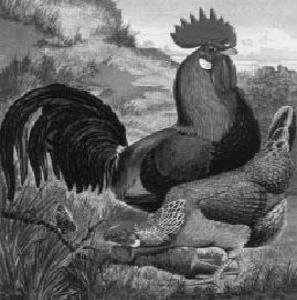
\includegraphics[scale=.35]{roosterrs-image_0001.jpg}
    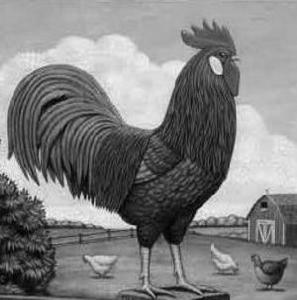
\includegraphics[scale=.35]{roosterrs-image_0002.jpg} \\
    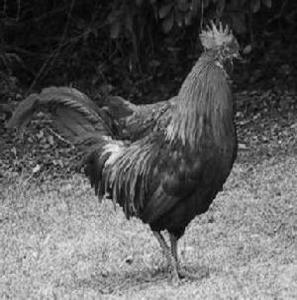
\includegraphics[scale=.35]{roosterrs-image_0003.jpg}
    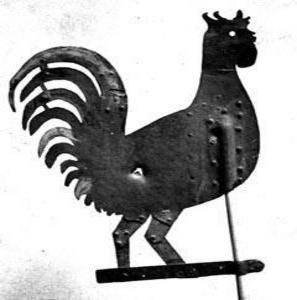
\includegraphics[scale=.35]{roosterrs-image_0004.jpg}
  \end{figure}
\end{frame}

\begin{frame}{Image Data (Pigeons)}
  \begin{figure}
    \centering
    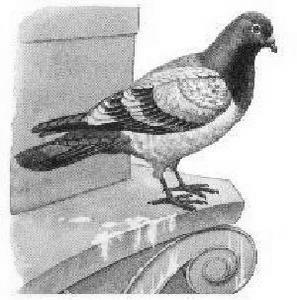
\includegraphics[scale=.35]{pigeonrs-image_0001.jpg}
    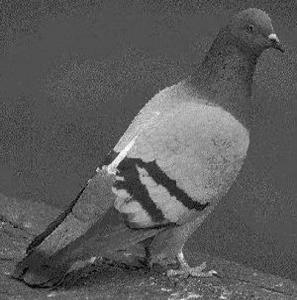
\includegraphics[scale=.35]{pigeonrs-image_0002.jpg} \\
    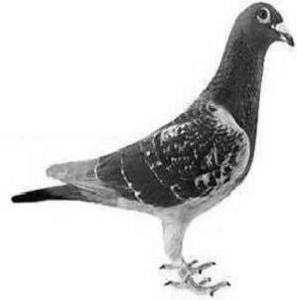
\includegraphics[scale=.35]{pigeonrs-image_0003.jpg}
    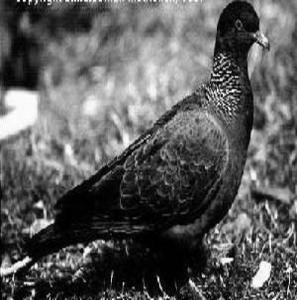
\includegraphics[scale=.35]{pigeonrs-image_0004.jpg}
  \end{figure}
\end{frame}

\begin{frame}{Polynomial Kernel}
  Compares 2 vectors (images) on products of elements (pixel intensities)
  up to a certain order.
  \begin{itemize}
    \item $\mathcal{X} = \mathbb{R}^{n}$ \pause
    \item $\phi_2 ([x_1, x_2]) = [x_1^2,  2x_1x_2,  x_2^2, \sqrt{2c}x_1, \sqrt{2c}x_2, c]$ \pause
    \item $\langle \phi_2({\bf x}), \phi_2({\bf y}) \rangle$ is $\mathcal{O}(n^2)$ \pause
    \item $\mathcal{V} = \mathbb{R}^{d'}$, where $d' = \binom{n+d}{d}$ \pause
    \item $K_d(x,y) = (x^T y  + c)^d$ is $\mathcal{O}(n)$
  \end{itemize}
\end{frame}

\begin{frame}{Rooster/Pigeon Example}
  \begin{center}
    \resizebox{10.0cm}{!}{
      % Created by tikzDevice version 0.6.2-92-0ad2792 on 2013-03-06 14:04:27
% !TEX encoding = UTF-8 Unicode
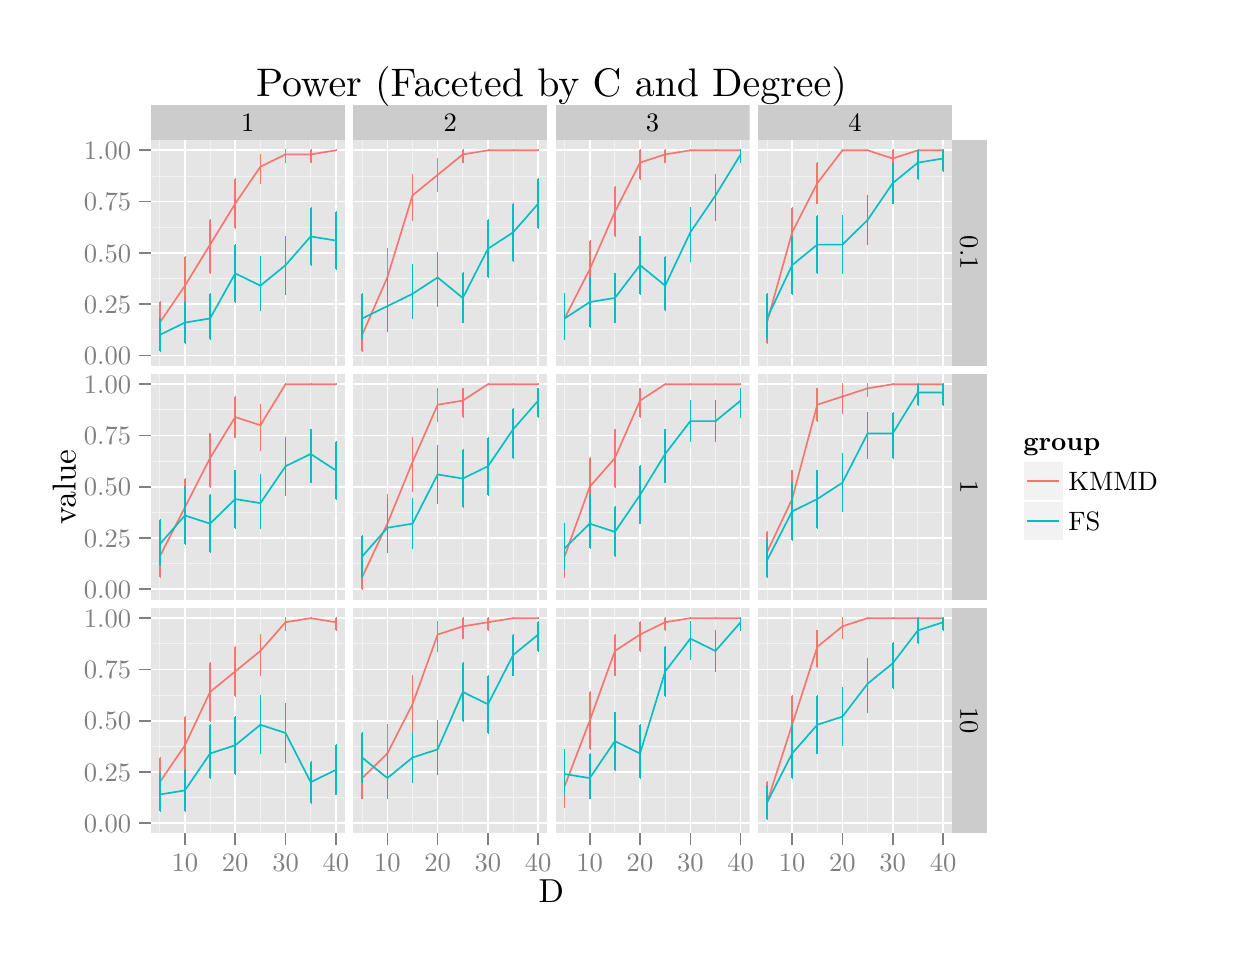
\begin{tikzpicture}[x=1pt,y=1pt]
\definecolor[named]{fillColor}{rgb}{1.00,1.00,1.00}
\path[use as bounding box,fill=fillColor,fill opacity=0.00] (0,0) rectangle (433.62,325.21);
\begin{scope}
\path[clip] (  0.00,  0.00) rectangle (433.62,325.21);
\definecolor[named]{drawColor}{rgb}{1.00,1.00,1.00}
\definecolor[named]{fillColor}{rgb}{1.00,1.00,1.00}

\path[draw=drawColor,line width= 0.6pt,line join=round,line cap=round,fill=fillColor] (  0.00,  0.00) rectangle (433.62,325.21);
\end{scope}
\begin{scope}
\path[clip] ( 44.49,284.60) rectangle (114.61,297.23);
\definecolor[named]{fillColor}{rgb}{0.80,0.80,0.80}

\path[fill=fillColor] ( 44.49,284.60) rectangle (114.61,297.23);
\definecolor[named]{drawColor}{rgb}{0.00,0.00,0.00}

\node[text=drawColor,anchor=base,inner sep=0pt, outer sep=0pt, scale=  0.96] at ( 79.55,287.61) {1};
\end{scope}
\begin{scope}
\path[clip] (117.62,284.60) rectangle (187.75,297.23);
\definecolor[named]{fillColor}{rgb}{0.80,0.80,0.80}

\path[fill=fillColor] (117.62,284.60) rectangle (187.75,297.23);
\definecolor[named]{drawColor}{rgb}{0.00,0.00,0.00}

\node[text=drawColor,anchor=base,inner sep=0pt, outer sep=0pt, scale=  0.96] at (152.68,287.61) {2};
\end{scope}
\begin{scope}
\path[clip] (190.76,284.60) rectangle (260.88,297.23);
\definecolor[named]{fillColor}{rgb}{0.80,0.80,0.80}

\path[fill=fillColor] (190.76,284.60) rectangle (260.88,297.23);
\definecolor[named]{drawColor}{rgb}{0.00,0.00,0.00}

\node[text=drawColor,anchor=base,inner sep=0pt, outer sep=0pt, scale=  0.96] at (225.82,287.61) {3};
\end{scope}
\begin{scope}
\path[clip] (263.89,284.60) rectangle (334.02,297.23);
\definecolor[named]{fillColor}{rgb}{0.80,0.80,0.80}

\path[fill=fillColor] (263.89,284.60) rectangle (334.02,297.23);
\definecolor[named]{drawColor}{rgb}{0.00,0.00,0.00}

\node[text=drawColor,anchor=base,inner sep=0pt, outer sep=0pt, scale=  0.96] at (298.95,287.61) {4};
\end{scope}
\begin{scope}
\path[clip] ( 44.49,203.08) rectangle (114.61,284.60);
\definecolor[named]{fillColor}{rgb}{0.90,0.90,0.90}

\path[fill=fillColor] ( 44.49,203.08) rectangle (114.61,284.60);
\definecolor[named]{drawColor}{rgb}{0.95,0.95,0.95}

\path[draw=drawColor,line width= 0.3pt,line join=round] ( 44.49,216.05) --
	(114.61,216.05);

\path[draw=drawColor,line width= 0.3pt,line join=round] ( 44.49,234.58) --
	(114.61,234.58);

\path[draw=drawColor,line width= 0.3pt,line join=round] ( 44.49,253.10) --
	(114.61,253.10);

\path[draw=drawColor,line width= 0.3pt,line join=round] ( 44.49,271.63) --
	(114.61,271.63);

\path[draw=drawColor,line width= 0.3pt,line join=round] ( 47.74,203.08) --
	( 47.74,284.60);

\path[draw=drawColor,line width= 0.3pt,line join=round] ( 65.91,203.08) --
	( 65.91,284.60);

\path[draw=drawColor,line width= 0.3pt,line join=round] ( 84.09,203.08) --
	( 84.09,284.60);

\path[draw=drawColor,line width= 0.3pt,line join=round] (102.27,203.08) --
	(102.27,284.60);
\definecolor[named]{drawColor}{rgb}{1.00,1.00,1.00}

\path[draw=drawColor,line width= 0.6pt,line join=round] ( 44.49,206.79) --
	(114.61,206.79);

\path[draw=drawColor,line width= 0.6pt,line join=round] ( 44.49,225.31) --
	(114.61,225.31);

\path[draw=drawColor,line width= 0.6pt,line join=round] ( 44.49,243.84) --
	(114.61,243.84);

\path[draw=drawColor,line width= 0.6pt,line join=round] ( 44.49,262.36) --
	(114.61,262.36);

\path[draw=drawColor,line width= 0.6pt,line join=round] ( 44.49,280.89) --
	(114.61,280.89);

\path[draw=drawColor,line width= 0.6pt,line join=round] ( 56.83,203.08) --
	( 56.83,284.60);

\path[draw=drawColor,line width= 0.6pt,line join=round] ( 75.00,203.08) --
	( 75.00,284.60);

\path[draw=drawColor,line width= 0.6pt,line join=round] ( 93.18,203.08) --
	( 93.18,284.60);

\path[draw=drawColor,line width= 0.6pt,line join=round] (111.36,203.08) --
	(111.36,284.60);
\definecolor[named]{drawColor}{rgb}{0.97,0.46,0.43}

\path[draw=drawColor,line width= 0.6pt,line join=round] ( 47.74,218.64) --
	( 56.83,231.98) --
	( 65.91,246.80) --
	( 75.00,261.62) --
	( 84.09,274.96) --
	( 93.18,279.41) --
	(102.27,279.41) --
	(111.36,280.89);
\definecolor[named]{drawColor}{rgb}{0.00,0.75,0.77}

\path[draw=drawColor,line width= 0.6pt,line join=round] ( 47.74,214.20) --
	( 56.83,218.64) --
	( 65.91,220.13) --
	( 75.00,236.43) --
	( 84.09,231.98) --
	( 93.18,239.39) --
	(102.27,249.77) --
	(111.36,248.29);
\definecolor[named]{drawColor}{rgb}{0.97,0.46,0.43}

\path[draw=drawColor,line width= 0.6pt,line join=round] ( 47.67,226.05) --
	( 47.80,226.05);

\path[draw=drawColor,line width= 0.6pt,line join=round] ( 47.74,226.05) --
	( 47.74,211.23);

\path[draw=drawColor,line width= 0.6pt,line join=round] ( 47.67,211.23) --
	( 47.80,211.23);

\path[draw=drawColor,line width= 0.6pt,line join=round] ( 56.76,242.36) --
	( 56.89,242.36);

\path[draw=drawColor,line width= 0.6pt,line join=round] ( 56.83,242.36) --
	( 56.83,223.09);

\path[draw=drawColor,line width= 0.6pt,line join=round] ( 56.76,223.09) --
	( 56.89,223.09);

\path[draw=drawColor,line width= 0.6pt,line join=round] ( 65.85,255.73) --
	( 65.98,255.73);

\path[draw=drawColor,line width= 0.6pt,line join=round] ( 65.91,255.73) --
	( 65.91,236.43);

\path[draw=drawColor,line width= 0.6pt,line join=round] ( 65.85,236.43) --
	( 65.98,236.43);

\path[draw=drawColor,line width= 0.6pt,line join=round] ( 74.94,270.52) --
	( 75.07,270.52);

\path[draw=drawColor,line width= 0.6pt,line join=round] ( 75.00,270.52) --
	( 75.00,252.73);

\path[draw=drawColor,line width= 0.6pt,line join=round] ( 74.94,252.73) --
	( 75.07,252.73);

\path[draw=drawColor,line width= 0.6pt,line join=round] ( 84.03,279.41) --
	( 84.16,279.41);

\path[draw=drawColor,line width= 0.6pt,line join=round] ( 84.09,279.41) --
	( 84.09,269.03);

\path[draw=drawColor,line width= 0.6pt,line join=round] ( 84.03,269.03) --
	( 84.16,269.03);

\path[draw=drawColor,line width= 0.6pt,line join=round] ( 93.12,280.89) --
	( 93.24,280.89);

\path[draw=drawColor,line width= 0.6pt,line join=round] ( 93.18,280.89) --
	( 93.18,276.44);

\path[draw=drawColor,line width= 0.6pt,line join=round] ( 93.12,276.44) --
	( 93.24,276.44);

\path[draw=drawColor,line width= 0.6pt,line join=round] (102.21,280.89) --
	(102.33,280.89);

\path[draw=drawColor,line width= 0.6pt,line join=round] (102.27,280.89) --
	(102.27,276.44);

\path[draw=drawColor,line width= 0.6pt,line join=round] (102.21,276.44) --
	(102.33,276.44);

\path[draw=drawColor,line width= 0.6pt,line join=round] (111.29,280.89) --
	(111.42,280.89);

\path[draw=drawColor,line width= 0.6pt,line join=round] (111.36,280.89) --
	(111.36,280.89);

\path[draw=drawColor,line width= 0.6pt,line join=round] (111.29,280.89) --
	(111.42,280.89);
\definecolor[named]{drawColor}{rgb}{0.00,0.75,0.77}

\path[draw=drawColor,line width= 0.6pt,line join=round] ( 47.67,220.13) --
	( 47.80,220.13);

\path[draw=drawColor,line width= 0.6pt,line join=round] ( 47.74,220.13) --
	( 47.74,208.27);

\path[draw=drawColor,line width= 0.6pt,line join=round] ( 47.67,208.27) --
	( 47.80,208.27);

\path[draw=drawColor,line width= 0.6pt,line join=round] ( 56.76,226.05) --
	( 56.89,226.05);

\path[draw=drawColor,line width= 0.6pt,line join=round] ( 56.83,226.05) --
	( 56.83,211.23);

\path[draw=drawColor,line width= 0.6pt,line join=round] ( 56.76,211.23) --
	( 56.89,211.23);

\path[draw=drawColor,line width= 0.6pt,line join=round] ( 65.85,229.02) --
	( 65.98,229.02);

\path[draw=drawColor,line width= 0.6pt,line join=round] ( 65.91,229.02) --
	( 65.91,212.72);

\path[draw=drawColor,line width= 0.6pt,line join=round] ( 65.85,212.72) --
	( 65.98,212.72);

\path[draw=drawColor,line width= 0.6pt,line join=round] ( 74.94,246.80) --
	( 75.07,246.80);

\path[draw=drawColor,line width= 0.6pt,line join=round] ( 75.00,246.80) --
	( 75.00,226.05);

\path[draw=drawColor,line width= 0.6pt,line join=round] ( 74.94,226.05) --
	( 75.07,226.05);

\path[draw=drawColor,line width= 0.6pt,line join=round] ( 84.03,242.36) --
	( 84.16,242.36);

\path[draw=drawColor,line width= 0.6pt,line join=round] ( 84.09,242.36) --
	( 84.09,223.09);

\path[draw=drawColor,line width= 0.6pt,line join=round] ( 84.03,223.09) --
	( 84.16,223.09);

\path[draw=drawColor,line width= 0.6pt,line join=round] ( 93.12,249.77) --
	( 93.24,249.77);

\path[draw=drawColor,line width= 0.6pt,line join=round] ( 93.18,249.77) --
	( 93.18,229.02);

\path[draw=drawColor,line width= 0.6pt,line join=round] ( 93.12,229.02) --
	( 93.24,229.02);

\path[draw=drawColor,line width= 0.6pt,line join=round] (102.21,260.14) --
	(102.33,260.14);

\path[draw=drawColor,line width= 0.6pt,line join=round] (102.27,260.14) --
	(102.27,239.39);

\path[draw=drawColor,line width= 0.6pt,line join=round] (102.21,239.39) --
	(102.33,239.39);

\path[draw=drawColor,line width= 0.6pt,line join=round] (111.29,258.66) --
	(111.42,258.66);

\path[draw=drawColor,line width= 0.6pt,line join=round] (111.36,258.66) --
	(111.36,237.91);

\path[draw=drawColor,line width= 0.6pt,line join=round] (111.29,237.91) --
	(111.42,237.91);
\end{scope}
\begin{scope}
\path[clip] ( 44.49,118.56) rectangle (114.61,200.07);
\definecolor[named]{fillColor}{rgb}{0.90,0.90,0.90}

\path[fill=fillColor] ( 44.49,118.56) rectangle (114.61,200.07);
\definecolor[named]{drawColor}{rgb}{0.95,0.95,0.95}

\path[draw=drawColor,line width= 0.3pt,line join=round] ( 44.49,131.53) --
	(114.61,131.53);

\path[draw=drawColor,line width= 0.3pt,line join=round] ( 44.49,150.05) --
	(114.61,150.05);

\path[draw=drawColor,line width= 0.3pt,line join=round] ( 44.49,168.58) --
	(114.61,168.58);

\path[draw=drawColor,line width= 0.3pt,line join=round] ( 44.49,187.10) --
	(114.61,187.10);

\path[draw=drawColor,line width= 0.3pt,line join=round] ( 47.74,118.56) --
	( 47.74,200.07);

\path[draw=drawColor,line width= 0.3pt,line join=round] ( 65.91,118.56) --
	( 65.91,200.07);

\path[draw=drawColor,line width= 0.3pt,line join=round] ( 84.09,118.56) --
	( 84.09,200.07);

\path[draw=drawColor,line width= 0.3pt,line join=round] (102.27,118.56) --
	(102.27,200.07);
\definecolor[named]{drawColor}{rgb}{1.00,1.00,1.00}

\path[draw=drawColor,line width= 0.6pt,line join=round] ( 44.49,122.26) --
	(114.61,122.26);

\path[draw=drawColor,line width= 0.6pt,line join=round] ( 44.49,140.79) --
	(114.61,140.79);

\path[draw=drawColor,line width= 0.6pt,line join=round] ( 44.49,159.32) --
	(114.61,159.32);

\path[draw=drawColor,line width= 0.6pt,line join=round] ( 44.49,177.84) --
	(114.61,177.84);

\path[draw=drawColor,line width= 0.6pt,line join=round] ( 44.49,196.37) --
	(114.61,196.37);

\path[draw=drawColor,line width= 0.6pt,line join=round] ( 56.83,118.56) --
	( 56.83,200.07);

\path[draw=drawColor,line width= 0.6pt,line join=round] ( 75.00,118.56) --
	( 75.00,200.07);

\path[draw=drawColor,line width= 0.6pt,line join=round] ( 93.18,118.56) --
	( 93.18,200.07);

\path[draw=drawColor,line width= 0.6pt,line join=round] (111.36,118.56) --
	(111.36,200.07);
\definecolor[named]{drawColor}{rgb}{0.97,0.46,0.43}

\path[draw=drawColor,line width= 0.6pt,line join=round] ( 47.74,134.12) --
	( 56.83,151.90) --
	( 65.91,169.69) --
	( 75.00,184.51) --
	( 84.09,181.55) --
	( 93.18,196.37) --
	(102.27,196.37) --
	(111.36,196.37);
\definecolor[named]{drawColor}{rgb}{0.00,0.75,0.77}

\path[draw=drawColor,line width= 0.6pt,line join=round] ( 47.74,138.57) --
	( 56.83,148.94) --
	( 65.91,145.98) --
	( 75.00,154.87) --
	( 84.09,153.39) --
	( 93.18,166.73) --
	(102.27,171.17) --
	(111.36,165.24);
\definecolor[named]{drawColor}{rgb}{0.97,0.46,0.43}

\path[draw=drawColor,line width= 0.6pt,line join=round] ( 47.67,143.01) --
	( 47.80,143.01);

\path[draw=drawColor,line width= 0.6pt,line join=round] ( 47.74,143.01) --
	( 47.74,126.71);

\path[draw=drawColor,line width= 0.6pt,line join=round] ( 47.67,126.71) --
	( 47.80,126.71);

\path[draw=drawColor,line width= 0.6pt,line join=round] ( 56.76,162.28) --
	( 56.89,162.28);

\path[draw=drawColor,line width= 0.6pt,line join=round] ( 56.83,162.28) --
	( 56.83,141.53);

\path[draw=drawColor,line width= 0.6pt,line join=round] ( 56.76,141.53) --
	( 56.89,141.53);

\path[draw=drawColor,line width= 0.6pt,line join=round] ( 65.85,178.58) --
	( 65.98,178.58);

\path[draw=drawColor,line width= 0.6pt,line join=round] ( 65.91,178.58) --
	( 65.91,159.32);

\path[draw=drawColor,line width= 0.6pt,line join=round] ( 65.85,159.32) --
	( 65.98,159.32);

\path[draw=drawColor,line width= 0.6pt,line join=round] ( 74.94,191.92) --
	( 75.07,191.92);

\path[draw=drawColor,line width= 0.6pt,line join=round] ( 75.00,191.92) --
	( 75.00,177.10);

\path[draw=drawColor,line width= 0.6pt,line join=round] ( 74.94,177.10) --
	( 75.07,177.10);

\path[draw=drawColor,line width= 0.6pt,line join=round] ( 84.03,188.96) --
	( 84.16,188.96);

\path[draw=drawColor,line width= 0.6pt,line join=round] ( 84.09,188.96) --
	( 84.09,172.65);

\path[draw=drawColor,line width= 0.6pt,line join=round] ( 84.03,172.65) --
	( 84.16,172.65);

\path[draw=drawColor,line width= 0.6pt,line join=round] ( 93.12,196.37) --
	( 93.24,196.37);

\path[draw=drawColor,line width= 0.6pt,line join=round] ( 93.18,196.37) --
	( 93.18,196.37);

\path[draw=drawColor,line width= 0.6pt,line join=round] ( 93.12,196.37) --
	( 93.24,196.37);

\path[draw=drawColor,line width= 0.6pt,line join=round] (102.21,196.37) --
	(102.33,196.37);

\path[draw=drawColor,line width= 0.6pt,line join=round] (102.27,196.37) --
	(102.27,196.37);

\path[draw=drawColor,line width= 0.6pt,line join=round] (102.21,196.37) --
	(102.33,196.37);

\path[draw=drawColor,line width= 0.6pt,line join=round] (111.29,196.37) --
	(111.42,196.37);

\path[draw=drawColor,line width= 0.6pt,line join=round] (111.36,196.37) --
	(111.36,196.37);

\path[draw=drawColor,line width= 0.6pt,line join=round] (111.29,196.37) --
	(111.42,196.37);
\definecolor[named]{drawColor}{rgb}{0.00,0.75,0.77}

\path[draw=drawColor,line width= 0.6pt,line join=round] ( 47.67,147.46) --
	( 47.80,147.46);

\path[draw=drawColor,line width= 0.6pt,line join=round] ( 47.74,147.46) --
	( 47.74,131.16);

\path[draw=drawColor,line width= 0.6pt,line join=round] ( 47.67,131.16) --
	( 47.80,131.16);

\path[draw=drawColor,line width= 0.6pt,line join=round] ( 56.76,159.32) --
	( 56.89,159.32);

\path[draw=drawColor,line width= 0.6pt,line join=round] ( 56.83,159.32) --
	( 56.83,138.57);

\path[draw=drawColor,line width= 0.6pt,line join=round] ( 56.76,138.57) --
	( 56.89,138.57);

\path[draw=drawColor,line width= 0.6pt,line join=round] ( 65.85,156.35) --
	( 65.98,156.35);

\path[draw=drawColor,line width= 0.6pt,line join=round] ( 65.91,156.35) --
	( 65.91,135.60);

\path[draw=drawColor,line width= 0.6pt,line join=round] ( 65.85,135.60) --
	( 65.98,135.60);

\path[draw=drawColor,line width= 0.6pt,line join=round] ( 74.94,165.24) --
	( 75.07,165.24);

\path[draw=drawColor,line width= 0.6pt,line join=round] ( 75.00,165.24) --
	( 75.00,144.49);

\path[draw=drawColor,line width= 0.6pt,line join=round] ( 74.94,144.49) --
	( 75.07,144.49);

\path[draw=drawColor,line width= 0.6pt,line join=round] ( 84.03,163.76) --
	( 84.16,163.76);

\path[draw=drawColor,line width= 0.6pt,line join=round] ( 84.09,163.76) --
	( 84.09,144.49);

\path[draw=drawColor,line width= 0.6pt,line join=round] ( 84.03,144.49) --
	( 84.16,144.49);

\path[draw=drawColor,line width= 0.6pt,line join=round] ( 93.12,177.10) --
	( 93.24,177.10);

\path[draw=drawColor,line width= 0.6pt,line join=round] ( 93.18,177.10) --
	( 93.18,156.35);

\path[draw=drawColor,line width= 0.6pt,line join=round] ( 93.12,156.35) --
	( 93.24,156.35);

\path[draw=drawColor,line width= 0.6pt,line join=round] (102.21,180.06) --
	(102.33,180.06);

\path[draw=drawColor,line width= 0.6pt,line join=round] (102.27,180.06) --
	(102.27,160.80);

\path[draw=drawColor,line width= 0.6pt,line join=round] (102.21,160.80) --
	(102.33,160.80);

\path[draw=drawColor,line width= 0.6pt,line join=round] (111.29,175.62) --
	(111.42,175.62);

\path[draw=drawColor,line width= 0.6pt,line join=round] (111.36,175.62) --
	(111.36,154.87);

\path[draw=drawColor,line width= 0.6pt,line join=round] (111.29,154.87) --
	(111.42,154.87);
\end{scope}
\begin{scope}
\path[clip] ( 44.49, 34.03) rectangle (114.61,115.55);
\definecolor[named]{fillColor}{rgb}{0.90,0.90,0.90}

\path[fill=fillColor] ( 44.49, 34.03) rectangle (114.61,115.55);
\definecolor[named]{drawColor}{rgb}{0.95,0.95,0.95}

\path[draw=drawColor,line width= 0.3pt,line join=round] ( 44.49, 47.00) --
	(114.61, 47.00);

\path[draw=drawColor,line width= 0.3pt,line join=round] ( 44.49, 65.53) --
	(114.61, 65.53);

\path[draw=drawColor,line width= 0.3pt,line join=round] ( 44.49, 84.05) --
	(114.61, 84.05);

\path[draw=drawColor,line width= 0.3pt,line join=round] ( 44.49,102.58) --
	(114.61,102.58);

\path[draw=drawColor,line width= 0.3pt,line join=round] ( 47.74, 34.03) --
	( 47.74,115.55);

\path[draw=drawColor,line width= 0.3pt,line join=round] ( 65.91, 34.03) --
	( 65.91,115.55);

\path[draw=drawColor,line width= 0.3pt,line join=round] ( 84.09, 34.03) --
	( 84.09,115.55);

\path[draw=drawColor,line width= 0.3pt,line join=round] (102.27, 34.03) --
	(102.27,115.55);
\definecolor[named]{drawColor}{rgb}{1.00,1.00,1.00}

\path[draw=drawColor,line width= 0.6pt,line join=round] ( 44.49, 37.74) --
	(114.61, 37.74);

\path[draw=drawColor,line width= 0.6pt,line join=round] ( 44.49, 56.27) --
	(114.61, 56.27);

\path[draw=drawColor,line width= 0.6pt,line join=round] ( 44.49, 74.79) --
	(114.61, 74.79);

\path[draw=drawColor,line width= 0.6pt,line join=round] ( 44.49, 93.32) --
	(114.61, 93.32);

\path[draw=drawColor,line width= 0.6pt,line join=round] ( 44.49,111.84) --
	(114.61,111.84);

\path[draw=drawColor,line width= 0.6pt,line join=round] ( 56.83, 34.03) --
	( 56.83,115.55);

\path[draw=drawColor,line width= 0.6pt,line join=round] ( 75.00, 34.03) --
	( 75.00,115.55);

\path[draw=drawColor,line width= 0.6pt,line join=round] ( 93.18, 34.03) --
	( 93.18,115.55);

\path[draw=drawColor,line width= 0.6pt,line join=round] (111.36, 34.03) --
	(111.36,115.55);
\definecolor[named]{drawColor}{rgb}{0.97,0.46,0.43}

\path[draw=drawColor,line width= 0.6pt,line join=round] ( 47.74, 52.56) --
	( 56.83, 65.90) --
	( 65.91, 85.17) --
	( 75.00, 92.58) --
	( 84.09, 99.99) --
	( 93.18,110.36) --
	(102.27,111.84) --
	(111.36,110.36);
\definecolor[named]{drawColor}{rgb}{0.00,0.75,0.77}

\path[draw=drawColor,line width= 0.6pt,line join=round] ( 47.74, 48.11) --
	( 56.83, 49.60) --
	( 65.91, 62.93) --
	( 75.00, 65.90) --
	( 84.09, 73.31) --
	( 93.18, 70.34) --
	(102.27, 52.56) --
	(111.36, 57.01);
\definecolor[named]{drawColor}{rgb}{0.97,0.46,0.43}

\path[draw=drawColor,line width= 0.6pt,line join=round] ( 47.67, 61.45) --
	( 47.80, 61.45);

\path[draw=drawColor,line width= 0.6pt,line join=round] ( 47.74, 61.45) --
	( 47.74, 45.15);

\path[draw=drawColor,line width= 0.6pt,line join=round] ( 47.67, 45.15) --
	( 47.80, 45.15);

\path[draw=drawColor,line width= 0.6pt,line join=round] ( 56.76, 76.27) --
	( 56.89, 76.27);

\path[draw=drawColor,line width= 0.6pt,line join=round] ( 56.83, 76.27) --
	( 56.83, 55.52);

\path[draw=drawColor,line width= 0.6pt,line join=round] ( 56.76, 55.52) --
	( 56.89, 55.52);

\path[draw=drawColor,line width= 0.6pt,line join=round] ( 65.85, 95.54) --
	( 65.98, 95.54);

\path[draw=drawColor,line width= 0.6pt,line join=round] ( 65.91, 95.54) --
	( 65.91, 74.79);

\path[draw=drawColor,line width= 0.6pt,line join=round] ( 65.85, 74.79) --
	( 65.98, 74.79);

\path[draw=drawColor,line width= 0.6pt,line join=round] ( 74.94,101.47) --
	( 75.07,101.47);

\path[draw=drawColor,line width= 0.6pt,line join=round] ( 75.00,101.47) --
	( 75.00, 83.68);

\path[draw=drawColor,line width= 0.6pt,line join=round] ( 74.94, 83.68) --
	( 75.07, 83.68);

\path[draw=drawColor,line width= 0.6pt,line join=round] ( 84.03,105.91) --
	( 84.16,105.91);

\path[draw=drawColor,line width= 0.6pt,line join=round] ( 84.09,105.91) --
	( 84.09, 91.09);

\path[draw=drawColor,line width= 0.6pt,line join=round] ( 84.03, 91.09) --
	( 84.16, 91.09);

\path[draw=drawColor,line width= 0.6pt,line join=round] ( 93.12,111.84) --
	( 93.24,111.84);

\path[draw=drawColor,line width= 0.6pt,line join=round] ( 93.18,111.84) --
	( 93.18,107.40);

\path[draw=drawColor,line width= 0.6pt,line join=round] ( 93.12,107.40) --
	( 93.24,107.40);

\path[draw=drawColor,line width= 0.6pt,line join=round] (102.21,111.84) --
	(102.33,111.84);

\path[draw=drawColor,line width= 0.6pt,line join=round] (102.27,111.84) --
	(102.27,111.84);

\path[draw=drawColor,line width= 0.6pt,line join=round] (102.21,111.84) --
	(102.33,111.84);

\path[draw=drawColor,line width= 0.6pt,line join=round] (111.29,111.84) --
	(111.42,111.84);

\path[draw=drawColor,line width= 0.6pt,line join=round] (111.36,111.84) --
	(111.36,107.40);

\path[draw=drawColor,line width= 0.6pt,line join=round] (111.29,107.40) --
	(111.42,107.40);
\definecolor[named]{drawColor}{rgb}{0.00,0.75,0.77}

\path[draw=drawColor,line width= 0.6pt,line join=round] ( 47.67, 55.52) --
	( 47.80, 55.52);

\path[draw=drawColor,line width= 0.6pt,line join=round] ( 47.74, 55.52) --
	( 47.74, 42.19);

\path[draw=drawColor,line width= 0.6pt,line join=round] ( 47.67, 42.19) --
	( 47.80, 42.19);

\path[draw=drawColor,line width= 0.6pt,line join=round] ( 56.76, 57.01) --
	( 56.89, 57.01);

\path[draw=drawColor,line width= 0.6pt,line join=round] ( 56.83, 57.01) --
	( 56.83, 42.19);

\path[draw=drawColor,line width= 0.6pt,line join=round] ( 56.76, 42.19) --
	( 56.89, 42.19);

\path[draw=drawColor,line width= 0.6pt,line join=round] ( 65.85, 73.31) --
	( 65.98, 73.31);

\path[draw=drawColor,line width= 0.6pt,line join=round] ( 65.91, 73.31) --
	( 65.91, 54.04);

\path[draw=drawColor,line width= 0.6pt,line join=round] ( 65.85, 54.04) --
	( 65.98, 54.04);

\path[draw=drawColor,line width= 0.6pt,line join=round] ( 74.94, 76.27) --
	( 75.07, 76.27);

\path[draw=drawColor,line width= 0.6pt,line join=round] ( 75.00, 76.27) --
	( 75.00, 55.52);

\path[draw=drawColor,line width= 0.6pt,line join=round] ( 74.94, 55.52) --
	( 75.07, 55.52);

\path[draw=drawColor,line width= 0.6pt,line join=round] ( 84.03, 83.68) --
	( 84.16, 83.68);

\path[draw=drawColor,line width= 0.6pt,line join=round] ( 84.09, 83.68) --
	( 84.09, 62.93);

\path[draw=drawColor,line width= 0.6pt,line join=round] ( 84.03, 62.93) --
	( 84.16, 62.93);

\path[draw=drawColor,line width= 0.6pt,line join=round] ( 93.12, 80.72) --
	( 93.24, 80.72);

\path[draw=drawColor,line width= 0.6pt,line join=round] ( 93.18, 80.72) --
	( 93.18, 59.97);

\path[draw=drawColor,line width= 0.6pt,line join=round] ( 93.12, 59.97) --
	( 93.24, 59.97);

\path[draw=drawColor,line width= 0.6pt,line join=round] (102.21, 59.97) --
	(102.33, 59.97);

\path[draw=drawColor,line width= 0.6pt,line join=round] (102.27, 59.97) --
	(102.27, 45.15);

\path[draw=drawColor,line width= 0.6pt,line join=round] (102.21, 45.15) --
	(102.33, 45.15);

\path[draw=drawColor,line width= 0.6pt,line join=round] (111.29, 65.90) --
	(111.42, 65.90);

\path[draw=drawColor,line width= 0.6pt,line join=round] (111.36, 65.90) --
	(111.36, 48.11);

\path[draw=drawColor,line width= 0.6pt,line join=round] (111.29, 48.11) --
	(111.42, 48.11);
\end{scope}
\begin{scope}
\path[clip] (117.62,203.08) rectangle (187.75,284.60);
\definecolor[named]{fillColor}{rgb}{0.90,0.90,0.90}

\path[fill=fillColor] (117.62,203.08) rectangle (187.75,284.60);
\definecolor[named]{drawColor}{rgb}{0.95,0.95,0.95}

\path[draw=drawColor,line width= 0.3pt,line join=round] (117.62,216.05) --
	(187.75,216.05);

\path[draw=drawColor,line width= 0.3pt,line join=round] (117.62,234.58) --
	(187.75,234.58);

\path[draw=drawColor,line width= 0.3pt,line join=round] (117.62,253.10) --
	(187.75,253.10);

\path[draw=drawColor,line width= 0.3pt,line join=round] (117.62,271.63) --
	(187.75,271.63);

\path[draw=drawColor,line width= 0.3pt,line join=round] (120.87,203.08) --
	(120.87,284.60);

\path[draw=drawColor,line width= 0.3pt,line join=round] (139.05,203.08) --
	(139.05,284.60);

\path[draw=drawColor,line width= 0.3pt,line join=round] (157.23,203.08) --
	(157.23,284.60);

\path[draw=drawColor,line width= 0.3pt,line join=round] (175.41,203.08) --
	(175.41,284.60);
\definecolor[named]{drawColor}{rgb}{1.00,1.00,1.00}

\path[draw=drawColor,line width= 0.6pt,line join=round] (117.62,206.79) --
	(187.75,206.79);

\path[draw=drawColor,line width= 0.6pt,line join=round] (117.62,225.31) --
	(187.75,225.31);

\path[draw=drawColor,line width= 0.6pt,line join=round] (117.62,243.84) --
	(187.75,243.84);

\path[draw=drawColor,line width= 0.6pt,line join=round] (117.62,262.36) --
	(187.75,262.36);

\path[draw=drawColor,line width= 0.6pt,line join=round] (117.62,280.89) --
	(187.75,280.89);

\path[draw=drawColor,line width= 0.6pt,line join=round] (129.96,203.08) --
	(129.96,284.60);

\path[draw=drawColor,line width= 0.6pt,line join=round] (148.14,203.08) --
	(148.14,284.60);

\path[draw=drawColor,line width= 0.6pt,line join=round] (166.32,203.08) --
	(166.32,284.60);

\path[draw=drawColor,line width= 0.6pt,line join=round] (184.49,203.08) --
	(184.49,284.60);
\definecolor[named]{drawColor}{rgb}{0.97,0.46,0.43}

\path[draw=drawColor,line width= 0.6pt,line join=round] (120.87,214.20) --
	(129.96,234.95) --
	(139.05,264.59) --
	(148.14,272.00) --
	(157.23,279.41) --
	(166.32,280.89) --
	(175.41,280.89) --
	(184.49,280.89);
\definecolor[named]{drawColor}{rgb}{0.00,0.75,0.77}

\path[draw=drawColor,line width= 0.6pt,line join=round] (120.87,220.13) --
	(129.96,224.57) --
	(139.05,229.02) --
	(148.14,234.95) --
	(157.23,227.54) --
	(166.32,245.32) --
	(175.41,251.25) --
	(184.49,261.62);
\definecolor[named]{drawColor}{rgb}{0.97,0.46,0.43}

\path[draw=drawColor,line width= 0.6pt,line join=round] (120.81,220.13) --
	(120.94,220.13);

\path[draw=drawColor,line width= 0.6pt,line join=round] (120.87,220.13) --
	(120.87,208.27);

\path[draw=drawColor,line width= 0.6pt,line join=round] (120.81,208.27) --
	(120.94,208.27);

\path[draw=drawColor,line width= 0.6pt,line join=round] (129.90,245.32) --
	(130.02,245.32);

\path[draw=drawColor,line width= 0.6pt,line join=round] (129.96,245.32) --
	(129.96,224.57);

\path[draw=drawColor,line width= 0.6pt,line join=round] (129.90,224.57) --
	(130.02,224.57);

\path[draw=drawColor,line width= 0.6pt,line join=round] (138.99,272.00) --
	(139.11,272.00);

\path[draw=drawColor,line width= 0.6pt,line join=round] (139.05,272.00) --
	(139.05,255.70);

\path[draw=drawColor,line width= 0.6pt,line join=round] (138.99,255.70) --
	(139.11,255.70);

\path[draw=drawColor,line width= 0.6pt,line join=round] (148.08,277.93) --
	(148.20,277.93);

\path[draw=drawColor,line width= 0.6pt,line join=round] (148.14,277.93) --
	(148.14,266.07);

\path[draw=drawColor,line width= 0.6pt,line join=round] (148.08,266.07) --
	(148.20,266.07);

\path[draw=drawColor,line width= 0.6pt,line join=round] (157.16,280.89) --
	(157.29,280.89);

\path[draw=drawColor,line width= 0.6pt,line join=round] (157.23,280.89) --
	(157.23,276.44);

\path[draw=drawColor,line width= 0.6pt,line join=round] (157.16,276.44) --
	(157.29,276.44);

\path[draw=drawColor,line width= 0.6pt,line join=round] (166.25,280.89) --
	(166.38,280.89);

\path[draw=drawColor,line width= 0.6pt,line join=round] (166.32,280.89) --
	(166.32,280.89);

\path[draw=drawColor,line width= 0.6pt,line join=round] (166.25,280.89) --
	(166.38,280.89);

\path[draw=drawColor,line width= 0.6pt,line join=round] (175.34,280.89) --
	(175.47,280.89);

\path[draw=drawColor,line width= 0.6pt,line join=round] (175.41,280.89) --
	(175.41,280.89);

\path[draw=drawColor,line width= 0.6pt,line join=round] (175.34,280.89) --
	(175.47,280.89);

\path[draw=drawColor,line width= 0.6pt,line join=round] (184.43,280.89) --
	(184.56,280.89);

\path[draw=drawColor,line width= 0.6pt,line join=round] (184.49,280.89) --
	(184.49,280.89);

\path[draw=drawColor,line width= 0.6pt,line join=round] (184.43,280.89) --
	(184.56,280.89);
\definecolor[named]{drawColor}{rgb}{0.00,0.75,0.77}

\path[draw=drawColor,line width= 0.6pt,line join=round] (120.81,229.02) --
	(120.94,229.02);

\path[draw=drawColor,line width= 0.6pt,line join=round] (120.87,229.02) --
	(120.87,212.72);

\path[draw=drawColor,line width= 0.6pt,line join=round] (120.81,212.72) --
	(120.94,212.72);

\path[draw=drawColor,line width= 0.6pt,line join=round] (129.90,234.95) --
	(130.02,234.95);

\path[draw=drawColor,line width= 0.6pt,line join=round] (129.96,234.95) --
	(129.96,215.68);

\path[draw=drawColor,line width= 0.6pt,line join=round] (129.90,215.68) --
	(130.02,215.68);

\path[draw=drawColor,line width= 0.6pt,line join=round] (138.99,239.39) --
	(139.11,239.39);

\path[draw=drawColor,line width= 0.6pt,line join=round] (139.05,239.39) --
	(139.05,220.13);

\path[draw=drawColor,line width= 0.6pt,line join=round] (138.99,220.13) --
	(139.11,220.13);

\path[draw=drawColor,line width= 0.6pt,line join=round] (148.08,243.84) --
	(148.20,243.84);

\path[draw=drawColor,line width= 0.6pt,line join=round] (148.14,243.84) --
	(148.14,224.57);

\path[draw=drawColor,line width= 0.6pt,line join=round] (148.08,224.57) --
	(148.20,224.57);

\path[draw=drawColor,line width= 0.6pt,line join=round] (157.16,236.47) --
	(157.29,236.47);

\path[draw=drawColor,line width= 0.6pt,line join=round] (157.23,236.47) --
	(157.23,218.64);

\path[draw=drawColor,line width= 0.6pt,line join=round] (157.16,218.64) --
	(157.29,218.64);

\path[draw=drawColor,line width= 0.6pt,line join=round] (166.25,255.70) --
	(166.38,255.70);

\path[draw=drawColor,line width= 0.6pt,line join=round] (166.32,255.70) --
	(166.32,234.95);

\path[draw=drawColor,line width= 0.6pt,line join=round] (166.25,234.95) --
	(166.38,234.95);

\path[draw=drawColor,line width= 0.6pt,line join=round] (175.34,261.62) --
	(175.47,261.62);

\path[draw=drawColor,line width= 0.6pt,line join=round] (175.41,261.62) --
	(175.41,240.88);

\path[draw=drawColor,line width= 0.6pt,line join=round] (175.34,240.88) --
	(175.47,240.88);

\path[draw=drawColor,line width= 0.6pt,line join=round] (184.43,270.52) --
	(184.56,270.52);

\path[draw=drawColor,line width= 0.6pt,line join=round] (184.49,270.52) --
	(184.49,252.73);

\path[draw=drawColor,line width= 0.6pt,line join=round] (184.43,252.73) --
	(184.56,252.73);
\end{scope}
\begin{scope}
\path[clip] (117.62,118.56) rectangle (187.75,200.07);
\definecolor[named]{fillColor}{rgb}{0.90,0.90,0.90}

\path[fill=fillColor] (117.62,118.56) rectangle (187.75,200.07);
\definecolor[named]{drawColor}{rgb}{0.95,0.95,0.95}

\path[draw=drawColor,line width= 0.3pt,line join=round] (117.62,131.53) --
	(187.75,131.53);

\path[draw=drawColor,line width= 0.3pt,line join=round] (117.62,150.05) --
	(187.75,150.05);

\path[draw=drawColor,line width= 0.3pt,line join=round] (117.62,168.58) --
	(187.75,168.58);

\path[draw=drawColor,line width= 0.3pt,line join=round] (117.62,187.10) --
	(187.75,187.10);

\path[draw=drawColor,line width= 0.3pt,line join=round] (120.87,118.56) --
	(120.87,200.07);

\path[draw=drawColor,line width= 0.3pt,line join=round] (139.05,118.56) --
	(139.05,200.07);

\path[draw=drawColor,line width= 0.3pt,line join=round] (157.23,118.56) --
	(157.23,200.07);

\path[draw=drawColor,line width= 0.3pt,line join=round] (175.41,118.56) --
	(175.41,200.07);
\definecolor[named]{drawColor}{rgb}{1.00,1.00,1.00}

\path[draw=drawColor,line width= 0.6pt,line join=round] (117.62,122.26) --
	(187.75,122.26);

\path[draw=drawColor,line width= 0.6pt,line join=round] (117.62,140.79) --
	(187.75,140.79);

\path[draw=drawColor,line width= 0.6pt,line join=round] (117.62,159.32) --
	(187.75,159.32);

\path[draw=drawColor,line width= 0.6pt,line join=round] (117.62,177.84) --
	(187.75,177.84);

\path[draw=drawColor,line width= 0.6pt,line join=round] (117.62,196.37) --
	(187.75,196.37);

\path[draw=drawColor,line width= 0.6pt,line join=round] (129.96,118.56) --
	(129.96,200.07);

\path[draw=drawColor,line width= 0.6pt,line join=round] (148.14,118.56) --
	(148.14,200.07);

\path[draw=drawColor,line width= 0.6pt,line join=round] (166.32,118.56) --
	(166.32,200.07);

\path[draw=drawColor,line width= 0.6pt,line join=round] (184.49,118.56) --
	(184.49,200.07);
\definecolor[named]{drawColor}{rgb}{0.97,0.46,0.43}

\path[draw=drawColor,line width= 0.6pt,line join=round] (120.87,126.71) --
	(129.96,145.98) --
	(139.05,168.21) --
	(148.14,188.96) --
	(157.23,190.44) --
	(166.32,196.37) --
	(175.41,196.37) --
	(184.49,196.37);
\definecolor[named]{drawColor}{rgb}{0.00,0.75,0.77}

\path[draw=drawColor,line width= 0.6pt,line join=round] (120.87,134.12) --
	(129.96,144.49) --
	(139.05,145.98) --
	(148.14,163.76) --
	(157.23,162.28) --
	(166.32,166.73) --
	(175.41,180.06) --
	(184.49,190.44);
\definecolor[named]{drawColor}{rgb}{0.97,0.46,0.43}

\path[draw=drawColor,line width= 0.6pt,line join=round] (120.81,132.64) --
	(120.94,132.64);

\path[draw=drawColor,line width= 0.6pt,line join=round] (120.87,132.64) --
	(120.87,122.26);

\path[draw=drawColor,line width= 0.6pt,line join=round] (120.81,122.26) --
	(120.94,122.26);

\path[draw=drawColor,line width= 0.6pt,line join=round] (129.90,156.35) --
	(130.02,156.35);

\path[draw=drawColor,line width= 0.6pt,line join=round] (129.96,156.35) --
	(129.96,137.08);

\path[draw=drawColor,line width= 0.6pt,line join=round] (129.90,137.08) --
	(130.02,137.08);

\path[draw=drawColor,line width= 0.6pt,line join=round] (138.99,177.10) --
	(139.11,177.10);

\path[draw=drawColor,line width= 0.6pt,line join=round] (139.05,177.10) --
	(139.05,157.83);

\path[draw=drawColor,line width= 0.6pt,line join=round] (138.99,157.83) --
	(139.11,157.83);

\path[draw=drawColor,line width= 0.6pt,line join=round] (148.08,194.88) --
	(148.20,194.88);

\path[draw=drawColor,line width= 0.6pt,line join=round] (148.14,194.88) --
	(148.14,183.03);

\path[draw=drawColor,line width= 0.6pt,line join=round] (148.08,183.03) --
	(148.20,183.03);

\path[draw=drawColor,line width= 0.6pt,line join=round] (157.16,194.88) --
	(157.29,194.88);

\path[draw=drawColor,line width= 0.6pt,line join=round] (157.23,194.88) --
	(157.23,184.51);

\path[draw=drawColor,line width= 0.6pt,line join=round] (157.16,184.51) --
	(157.29,184.51);

\path[draw=drawColor,line width= 0.6pt,line join=round] (166.25,196.37) --
	(166.38,196.37);

\path[draw=drawColor,line width= 0.6pt,line join=round] (166.32,196.37) --
	(166.32,196.37);

\path[draw=drawColor,line width= 0.6pt,line join=round] (166.25,196.37) --
	(166.38,196.37);

\path[draw=drawColor,line width= 0.6pt,line join=round] (175.34,196.37) --
	(175.47,196.37);

\path[draw=drawColor,line width= 0.6pt,line join=round] (175.41,196.37) --
	(175.41,196.37);

\path[draw=drawColor,line width= 0.6pt,line join=round] (175.34,196.37) --
	(175.47,196.37);

\path[draw=drawColor,line width= 0.6pt,line join=round] (184.43,196.37) --
	(184.56,196.37);

\path[draw=drawColor,line width= 0.6pt,line join=round] (184.49,196.37) --
	(184.49,196.37);

\path[draw=drawColor,line width= 0.6pt,line join=round] (184.43,196.37) --
	(184.56,196.37);
\definecolor[named]{drawColor}{rgb}{0.00,0.75,0.77}

\path[draw=drawColor,line width= 0.6pt,line join=round] (120.81,141.53) --
	(120.94,141.53);

\path[draw=drawColor,line width= 0.6pt,line join=round] (120.87,141.53) --
	(120.87,126.71);

\path[draw=drawColor,line width= 0.6pt,line join=round] (120.81,126.71) --
	(120.94,126.71);

\path[draw=drawColor,line width= 0.6pt,line join=round] (129.90,154.87) --
	(130.02,154.87);

\path[draw=drawColor,line width= 0.6pt,line join=round] (129.96,154.87) --
	(129.96,135.60);

\path[draw=drawColor,line width= 0.6pt,line join=round] (129.90,135.60) --
	(130.02,135.60);

\path[draw=drawColor,line width= 0.6pt,line join=round] (138.99,154.87) --
	(139.11,154.87);

\path[draw=drawColor,line width= 0.6pt,line join=round] (139.05,154.87) --
	(139.05,137.08);

\path[draw=drawColor,line width= 0.6pt,line join=round] (138.99,137.08) --
	(139.11,137.08);

\path[draw=drawColor,line width= 0.6pt,line join=round] (148.08,174.14) --
	(148.20,174.14);

\path[draw=drawColor,line width= 0.6pt,line join=round] (148.14,174.14) --
	(148.14,153.39);

\path[draw=drawColor,line width= 0.6pt,line join=round] (148.08,153.39) --
	(148.20,153.39);

\path[draw=drawColor,line width= 0.6pt,line join=round] (157.16,172.65) --
	(157.29,172.65);

\path[draw=drawColor,line width= 0.6pt,line join=round] (157.23,172.65) --
	(157.23,151.90);

\path[draw=drawColor,line width= 0.6pt,line join=round] (157.16,151.90) --
	(157.29,151.90);

\path[draw=drawColor,line width= 0.6pt,line join=round] (166.25,177.10) --
	(166.38,177.10);

\path[draw=drawColor,line width= 0.6pt,line join=round] (166.32,177.10) --
	(166.32,156.35);

\path[draw=drawColor,line width= 0.6pt,line join=round] (166.25,156.35) --
	(166.38,156.35);

\path[draw=drawColor,line width= 0.6pt,line join=round] (175.34,187.47) --
	(175.47,187.47);

\path[draw=drawColor,line width= 0.6pt,line join=round] (175.41,187.47) --
	(175.41,169.69);

\path[draw=drawColor,line width= 0.6pt,line join=round] (175.34,169.69) --
	(175.47,169.69);

\path[draw=drawColor,line width= 0.6pt,line join=round] (184.43,194.88) --
	(184.56,194.88);

\path[draw=drawColor,line width= 0.6pt,line join=round] (184.49,194.88) --
	(184.49,184.51);

\path[draw=drawColor,line width= 0.6pt,line join=round] (184.43,184.51) --
	(184.56,184.51);
\end{scope}
\begin{scope}
\path[clip] (117.62, 34.03) rectangle (187.75,115.55);
\definecolor[named]{fillColor}{rgb}{0.90,0.90,0.90}

\path[fill=fillColor] (117.62, 34.03) rectangle (187.75,115.55);
\definecolor[named]{drawColor}{rgb}{0.95,0.95,0.95}

\path[draw=drawColor,line width= 0.3pt,line join=round] (117.62, 47.00) --
	(187.75, 47.00);

\path[draw=drawColor,line width= 0.3pt,line join=round] (117.62, 65.53) --
	(187.75, 65.53);

\path[draw=drawColor,line width= 0.3pt,line join=round] (117.62, 84.05) --
	(187.75, 84.05);

\path[draw=drawColor,line width= 0.3pt,line join=round] (117.62,102.58) --
	(187.75,102.58);

\path[draw=drawColor,line width= 0.3pt,line join=round] (120.87, 34.03) --
	(120.87,115.55);

\path[draw=drawColor,line width= 0.3pt,line join=round] (139.05, 34.03) --
	(139.05,115.55);

\path[draw=drawColor,line width= 0.3pt,line join=round] (157.23, 34.03) --
	(157.23,115.55);

\path[draw=drawColor,line width= 0.3pt,line join=round] (175.41, 34.03) --
	(175.41,115.55);
\definecolor[named]{drawColor}{rgb}{1.00,1.00,1.00}

\path[draw=drawColor,line width= 0.6pt,line join=round] (117.62, 37.74) --
	(187.75, 37.74);

\path[draw=drawColor,line width= 0.6pt,line join=round] (117.62, 56.27) --
	(187.75, 56.27);

\path[draw=drawColor,line width= 0.6pt,line join=round] (117.62, 74.79) --
	(187.75, 74.79);

\path[draw=drawColor,line width= 0.6pt,line join=round] (117.62, 93.32) --
	(187.75, 93.32);

\path[draw=drawColor,line width= 0.6pt,line join=round] (117.62,111.84) --
	(187.75,111.84);

\path[draw=drawColor,line width= 0.6pt,line join=round] (129.96, 34.03) --
	(129.96,115.55);

\path[draw=drawColor,line width= 0.6pt,line join=round] (148.14, 34.03) --
	(148.14,115.55);

\path[draw=drawColor,line width= 0.6pt,line join=round] (166.32, 34.03) --
	(166.32,115.55);

\path[draw=drawColor,line width= 0.6pt,line join=round] (184.49, 34.03) --
	(184.49,115.55);
\definecolor[named]{drawColor}{rgb}{0.97,0.46,0.43}

\path[draw=drawColor,line width= 0.6pt,line join=round] (120.87, 54.04) --
	(129.96, 62.93) --
	(139.05, 80.72) --
	(148.14,105.91) --
	(157.23,108.88) --
	(166.32,110.36) --
	(175.41,111.84) --
	(184.49,111.84);
\definecolor[named]{drawColor}{rgb}{0.00,0.75,0.77}

\path[draw=drawColor,line width= 0.6pt,line join=round] (120.87, 61.45) --
	(129.96, 54.04) --
	(139.05, 61.45) --
	(148.14, 64.42) --
	(157.23, 85.17) --
	(166.32, 80.72) --
	(175.41, 98.50) --
	(184.49,105.91);
\definecolor[named]{drawColor}{rgb}{0.97,0.46,0.43}

\path[draw=drawColor,line width= 0.6pt,line join=round] (120.81, 62.93) --
	(120.94, 62.93);

\path[draw=drawColor,line width= 0.6pt,line join=round] (120.87, 62.93) --
	(120.87, 46.63);

\path[draw=drawColor,line width= 0.6pt,line join=round] (120.81, 46.63) --
	(120.94, 46.63);

\path[draw=drawColor,line width= 0.6pt,line join=round] (129.90, 73.31) --
	(130.02, 73.31);

\path[draw=drawColor,line width= 0.6pt,line join=round] (129.96, 73.31) --
	(129.96, 54.04);

\path[draw=drawColor,line width= 0.6pt,line join=round] (129.90, 54.04) --
	(130.02, 54.04);

\path[draw=drawColor,line width= 0.6pt,line join=round] (138.99, 91.09) --
	(139.11, 91.09);

\path[draw=drawColor,line width= 0.6pt,line join=round] (139.05, 91.09) --
	(139.05, 70.34);

\path[draw=drawColor,line width= 0.6pt,line join=round] (138.99, 70.34) --
	(139.11, 70.34);

\path[draw=drawColor,line width= 0.6pt,line join=round] (148.08,110.36) --
	(148.20,110.36);

\path[draw=drawColor,line width= 0.6pt,line join=round] (148.14,110.36) --
	(148.14, 99.99);

\path[draw=drawColor,line width= 0.6pt,line join=round] (148.08, 99.99) --
	(148.20, 99.99);

\path[draw=drawColor,line width= 0.6pt,line join=round] (157.16,111.84) --
	(157.29,111.84);

\path[draw=drawColor,line width= 0.6pt,line join=round] (157.23,111.84) --
	(157.23,104.43);

\path[draw=drawColor,line width= 0.6pt,line join=round] (157.16,104.43) --
	(157.29,104.43);

\path[draw=drawColor,line width= 0.6pt,line join=round] (166.25,111.84) --
	(166.38,111.84);

\path[draw=drawColor,line width= 0.6pt,line join=round] (166.32,111.84) --
	(166.32,107.40);

\path[draw=drawColor,line width= 0.6pt,line join=round] (166.25,107.40) --
	(166.38,107.40);

\path[draw=drawColor,line width= 0.6pt,line join=round] (175.34,111.84) --
	(175.47,111.84);

\path[draw=drawColor,line width= 0.6pt,line join=round] (175.41,111.84) --
	(175.41,111.84);

\path[draw=drawColor,line width= 0.6pt,line join=round] (175.34,111.84) --
	(175.47,111.84);

\path[draw=drawColor,line width= 0.6pt,line join=round] (184.43,111.84) --
	(184.56,111.84);

\path[draw=drawColor,line width= 0.6pt,line join=round] (184.49,111.84) --
	(184.49,111.84);

\path[draw=drawColor,line width= 0.6pt,line join=round] (184.43,111.84) --
	(184.56,111.84);
\definecolor[named]{drawColor}{rgb}{0.00,0.75,0.77}

\path[draw=drawColor,line width= 0.6pt,line join=round] (120.81, 70.34) --
	(120.94, 70.34);

\path[draw=drawColor,line width= 0.6pt,line join=round] (120.87, 70.34) --
	(120.87, 52.56);

\path[draw=drawColor,line width= 0.6pt,line join=round] (120.81, 52.56) --
	(120.94, 52.56);

\path[draw=drawColor,line width= 0.6pt,line join=round] (129.90, 62.93) --
	(130.02, 62.93);

\path[draw=drawColor,line width= 0.6pt,line join=round] (129.96, 62.93) --
	(129.96, 46.63);

\path[draw=drawColor,line width= 0.6pt,line join=round] (129.90, 46.63) --
	(130.02, 46.63);

\path[draw=drawColor,line width= 0.6pt,line join=round] (138.99, 70.34) --
	(139.11, 70.34);

\path[draw=drawColor,line width= 0.6pt,line join=round] (139.05, 70.34) --
	(139.05, 52.56);

\path[draw=drawColor,line width= 0.6pt,line join=round] (138.99, 52.56) --
	(139.11, 52.56);

\path[draw=drawColor,line width= 0.6pt,line join=round] (148.08, 74.79) --
	(148.20, 74.79);

\path[draw=drawColor,line width= 0.6pt,line join=round] (148.14, 74.79) --
	(148.14, 55.49);

\path[draw=drawColor,line width= 0.6pt,line join=round] (148.08, 55.49) --
	(148.20, 55.49);

\path[draw=drawColor,line width= 0.6pt,line join=round] (157.16, 95.54) --
	(157.29, 95.54);

\path[draw=drawColor,line width= 0.6pt,line join=round] (157.23, 95.54) --
	(157.23, 74.79);

\path[draw=drawColor,line width= 0.6pt,line join=round] (157.16, 74.79) --
	(157.29, 74.79);

\path[draw=drawColor,line width= 0.6pt,line join=round] (166.25, 91.09) --
	(166.38, 91.09);

\path[draw=drawColor,line width= 0.6pt,line join=round] (166.32, 91.09) --
	(166.32, 70.34);

\path[draw=drawColor,line width= 0.6pt,line join=round] (166.25, 70.34) --
	(166.38, 70.34);

\path[draw=drawColor,line width= 0.6pt,line join=round] (175.34,105.91) --
	(175.47,105.91);

\path[draw=drawColor,line width= 0.6pt,line join=round] (175.41,105.91) --
	(175.41, 91.09);

\path[draw=drawColor,line width= 0.6pt,line join=round] (175.34, 91.09) --
	(175.47, 91.09);

\path[draw=drawColor,line width= 0.6pt,line join=round] (184.43,110.36) --
	(184.56,110.36);

\path[draw=drawColor,line width= 0.6pt,line join=round] (184.49,110.36) --
	(184.49, 99.99);

\path[draw=drawColor,line width= 0.6pt,line join=round] (184.43, 99.99) --
	(184.56, 99.99);
\end{scope}
\begin{scope}
\path[clip] (190.76,203.08) rectangle (260.88,284.60);
\definecolor[named]{fillColor}{rgb}{0.90,0.90,0.90}

\path[fill=fillColor] (190.76,203.08) rectangle (260.88,284.60);
\definecolor[named]{drawColor}{rgb}{0.95,0.95,0.95}

\path[draw=drawColor,line width= 0.3pt,line join=round] (190.76,216.05) --
	(260.88,216.05);

\path[draw=drawColor,line width= 0.3pt,line join=round] (190.76,234.58) --
	(260.88,234.58);

\path[draw=drawColor,line width= 0.3pt,line join=round] (190.76,253.10) --
	(260.88,253.10);

\path[draw=drawColor,line width= 0.3pt,line join=round] (190.76,271.63) --
	(260.88,271.63);

\path[draw=drawColor,line width= 0.3pt,line join=round] (194.01,203.08) --
	(194.01,284.60);

\path[draw=drawColor,line width= 0.3pt,line join=round] (212.19,203.08) --
	(212.19,284.60);

\path[draw=drawColor,line width= 0.3pt,line join=round] (230.36,203.08) --
	(230.36,284.60);

\path[draw=drawColor,line width= 0.3pt,line join=round] (248.54,203.08) --
	(248.54,284.60);
\definecolor[named]{drawColor}{rgb}{1.00,1.00,1.00}

\path[draw=drawColor,line width= 0.6pt,line join=round] (190.76,206.79) --
	(260.88,206.79);

\path[draw=drawColor,line width= 0.6pt,line join=round] (190.76,225.31) --
	(260.88,225.31);

\path[draw=drawColor,line width= 0.6pt,line join=round] (190.76,243.84) --
	(260.88,243.84);

\path[draw=drawColor,line width= 0.6pt,line join=round] (190.76,262.36) --
	(260.88,262.36);

\path[draw=drawColor,line width= 0.6pt,line join=round] (190.76,280.89) --
	(260.88,280.89);

\path[draw=drawColor,line width= 0.6pt,line join=round] (203.10,203.08) --
	(203.10,284.60);

\path[draw=drawColor,line width= 0.6pt,line join=round] (221.27,203.08) --
	(221.27,284.60);

\path[draw=drawColor,line width= 0.6pt,line join=round] (239.45,203.08) --
	(239.45,284.60);

\path[draw=drawColor,line width= 0.6pt,line join=round] (257.63,203.08) --
	(257.63,284.60);
\definecolor[named]{drawColor}{rgb}{0.97,0.46,0.43}

\path[draw=drawColor,line width= 0.6pt,line join=round] (194.01,220.13) --
	(203.10,237.91) --
	(212.19,258.66) --
	(221.27,276.44) --
	(230.36,279.41) --
	(239.45,280.89) --
	(248.54,280.89) --
	(257.63,280.89);
\definecolor[named]{drawColor}{rgb}{0.00,0.75,0.77}

\path[draw=drawColor,line width= 0.6pt,line join=round] (194.01,220.13) --
	(203.10,226.05) --
	(212.19,227.54) --
	(221.27,239.39) --
	(230.36,231.98) --
	(239.45,251.25) --
	(248.54,264.59) --
	(257.63,279.41);
\definecolor[named]{drawColor}{rgb}{0.97,0.46,0.43}

\path[draw=drawColor,line width= 0.6pt,line join=round] (193.94,229.02) --
	(194.07,229.02);

\path[draw=drawColor,line width= 0.6pt,line join=round] (194.01,229.02) --
	(194.01,212.72);

\path[draw=drawColor,line width= 0.6pt,line join=round] (193.94,212.72) --
	(194.07,212.72);

\path[draw=drawColor,line width= 0.6pt,line join=round] (203.03,248.29) --
	(203.16,248.29);

\path[draw=drawColor,line width= 0.6pt,line join=round] (203.10,248.29) --
	(203.10,227.54);

\path[draw=drawColor,line width= 0.6pt,line join=round] (203.03,227.54) --
	(203.16,227.54);

\path[draw=drawColor,line width= 0.6pt,line join=round] (212.12,267.55) --
	(212.25,267.55);

\path[draw=drawColor,line width= 0.6pt,line join=round] (212.19,267.55) --
	(212.19,249.77);

\path[draw=drawColor,line width= 0.6pt,line join=round] (212.12,249.77) --
	(212.25,249.77);

\path[draw=drawColor,line width= 0.6pt,line join=round] (221.21,280.89) --
	(221.34,280.89);

\path[draw=drawColor,line width= 0.6pt,line join=round] (221.27,280.89) --
	(221.27,270.52);

\path[draw=drawColor,line width= 0.6pt,line join=round] (221.21,270.52) --
	(221.34,270.52);

\path[draw=drawColor,line width= 0.6pt,line join=round] (230.30,280.89) --
	(230.43,280.89);

\path[draw=drawColor,line width= 0.6pt,line join=round] (230.36,280.89) --
	(230.36,276.44);

\path[draw=drawColor,line width= 0.6pt,line join=round] (230.30,276.44) --
	(230.43,276.44);

\path[draw=drawColor,line width= 0.6pt,line join=round] (239.39,280.89) --
	(239.52,280.89);

\path[draw=drawColor,line width= 0.6pt,line join=round] (239.45,280.89) --
	(239.45,280.89);

\path[draw=drawColor,line width= 0.6pt,line join=round] (239.39,280.89) --
	(239.52,280.89);

\path[draw=drawColor,line width= 0.6pt,line join=round] (248.48,280.89) --
	(248.60,280.89);

\path[draw=drawColor,line width= 0.6pt,line join=round] (248.54,280.89) --
	(248.54,280.89);

\path[draw=drawColor,line width= 0.6pt,line join=round] (248.48,280.89) --
	(248.60,280.89);

\path[draw=drawColor,line width= 0.6pt,line join=round] (257.57,280.89) --
	(257.69,280.89);

\path[draw=drawColor,line width= 0.6pt,line join=round] (257.63,280.89) --
	(257.63,280.89);

\path[draw=drawColor,line width= 0.6pt,line join=round] (257.57,280.89) --
	(257.69,280.89);
\definecolor[named]{drawColor}{rgb}{0.00,0.75,0.77}

\path[draw=drawColor,line width= 0.6pt,line join=round] (193.94,229.02) --
	(194.07,229.02);

\path[draw=drawColor,line width= 0.6pt,line join=round] (194.01,229.02) --
	(194.01,212.72);

\path[draw=drawColor,line width= 0.6pt,line join=round] (193.94,212.72) --
	(194.07,212.72);

\path[draw=drawColor,line width= 0.6pt,line join=round] (203.03,234.95) --
	(203.16,234.95);

\path[draw=drawColor,line width= 0.6pt,line join=round] (203.10,234.95) --
	(203.10,217.16);

\path[draw=drawColor,line width= 0.6pt,line join=round] (203.03,217.16) --
	(203.16,217.16);

\path[draw=drawColor,line width= 0.6pt,line join=round] (212.12,236.43) --
	(212.25,236.43);

\path[draw=drawColor,line width= 0.6pt,line join=round] (212.19,236.43) --
	(212.19,218.64);

\path[draw=drawColor,line width= 0.6pt,line join=round] (212.12,218.64) --
	(212.25,218.64);

\path[draw=drawColor,line width= 0.6pt,line join=round] (221.21,249.77) --
	(221.34,249.77);

\path[draw=drawColor,line width= 0.6pt,line join=round] (221.27,249.77) --
	(221.27,229.02);

\path[draw=drawColor,line width= 0.6pt,line join=round] (221.21,229.02) --
	(221.34,229.02);

\path[draw=drawColor,line width= 0.6pt,line join=round] (230.30,242.36) --
	(230.43,242.36);

\path[draw=drawColor,line width= 0.6pt,line join=round] (230.36,242.36) --
	(230.36,223.09);

\path[draw=drawColor,line width= 0.6pt,line join=round] (230.30,223.09) --
	(230.43,223.09);

\path[draw=drawColor,line width= 0.6pt,line join=round] (239.39,260.14) --
	(239.52,260.14);

\path[draw=drawColor,line width= 0.6pt,line join=round] (239.45,260.14) --
	(239.45,240.88);

\path[draw=drawColor,line width= 0.6pt,line join=round] (239.39,240.88) --
	(239.52,240.88);

\path[draw=drawColor,line width= 0.6pt,line join=round] (248.48,272.00) --
	(248.60,272.00);

\path[draw=drawColor,line width= 0.6pt,line join=round] (248.54,272.00) --
	(248.54,255.70);

\path[draw=drawColor,line width= 0.6pt,line join=round] (248.48,255.70) --
	(248.60,255.70);

\path[draw=drawColor,line width= 0.6pt,line join=round] (257.57,280.89) --
	(257.69,280.89);

\path[draw=drawColor,line width= 0.6pt,line join=round] (257.63,280.89) --
	(257.63,276.44);

\path[draw=drawColor,line width= 0.6pt,line join=round] (257.57,276.44) --
	(257.69,276.44);
\end{scope}
\begin{scope}
\path[clip] (190.76,118.56) rectangle (260.88,200.07);
\definecolor[named]{fillColor}{rgb}{0.90,0.90,0.90}

\path[fill=fillColor] (190.76,118.56) rectangle (260.88,200.07);
\definecolor[named]{drawColor}{rgb}{0.95,0.95,0.95}

\path[draw=drawColor,line width= 0.3pt,line join=round] (190.76,131.53) --
	(260.88,131.53);

\path[draw=drawColor,line width= 0.3pt,line join=round] (190.76,150.05) --
	(260.88,150.05);

\path[draw=drawColor,line width= 0.3pt,line join=round] (190.76,168.58) --
	(260.88,168.58);

\path[draw=drawColor,line width= 0.3pt,line join=round] (190.76,187.10) --
	(260.88,187.10);

\path[draw=drawColor,line width= 0.3pt,line join=round] (194.01,118.56) --
	(194.01,200.07);

\path[draw=drawColor,line width= 0.3pt,line join=round] (212.19,118.56) --
	(212.19,200.07);

\path[draw=drawColor,line width= 0.3pt,line join=round] (230.36,118.56) --
	(230.36,200.07);

\path[draw=drawColor,line width= 0.3pt,line join=round] (248.54,118.56) --
	(248.54,200.07);
\definecolor[named]{drawColor}{rgb}{1.00,1.00,1.00}

\path[draw=drawColor,line width= 0.6pt,line join=round] (190.76,122.26) --
	(260.88,122.26);

\path[draw=drawColor,line width= 0.6pt,line join=round] (190.76,140.79) --
	(260.88,140.79);

\path[draw=drawColor,line width= 0.6pt,line join=round] (190.76,159.32) --
	(260.88,159.32);

\path[draw=drawColor,line width= 0.6pt,line join=round] (190.76,177.84) --
	(260.88,177.84);

\path[draw=drawColor,line width= 0.6pt,line join=round] (190.76,196.37) --
	(260.88,196.37);

\path[draw=drawColor,line width= 0.6pt,line join=round] (203.10,118.56) --
	(203.10,200.07);

\path[draw=drawColor,line width= 0.6pt,line join=round] (221.27,118.56) --
	(221.27,200.07);

\path[draw=drawColor,line width= 0.6pt,line join=round] (239.45,118.56) --
	(239.45,200.07);

\path[draw=drawColor,line width= 0.6pt,line join=round] (257.63,118.56) --
	(257.63,200.07);
\definecolor[named]{drawColor}{rgb}{0.97,0.46,0.43}

\path[draw=drawColor,line width= 0.6pt,line join=round] (194.01,134.12) --
	(203.10,159.32) --
	(212.19,169.69) --
	(221.27,190.44) --
	(230.36,196.37) --
	(239.45,196.37) --
	(248.54,196.37) --
	(257.63,196.37);
\definecolor[named]{drawColor}{rgb}{0.00,0.75,0.77}

\path[draw=drawColor,line width= 0.6pt,line join=round] (194.01,137.08) --
	(203.10,145.98) --
	(212.19,143.01) --
	(221.27,156.35) --
	(230.36,171.17) --
	(239.45,183.03) --
	(248.54,183.03) --
	(257.63,190.44);
\definecolor[named]{drawColor}{rgb}{0.97,0.46,0.43}

\path[draw=drawColor,line width= 0.6pt,line join=round] (193.94,141.53) --
	(194.07,141.53);

\path[draw=drawColor,line width= 0.6pt,line join=round] (194.01,141.53) --
	(194.01,126.71);

\path[draw=drawColor,line width= 0.6pt,line join=round] (193.94,126.71) --
	(194.07,126.71);

\path[draw=drawColor,line width= 0.6pt,line join=round] (203.03,169.69) --
	(203.16,169.69);

\path[draw=drawColor,line width= 0.6pt,line join=round] (203.10,169.69) --
	(203.10,150.42);

\path[draw=drawColor,line width= 0.6pt,line join=round] (203.03,150.42) --
	(203.16,150.42);

\path[draw=drawColor,line width= 0.6pt,line join=round] (212.12,180.06) --
	(212.25,180.06);

\path[draw=drawColor,line width= 0.6pt,line join=round] (212.19,180.06) --
	(212.19,159.32);

\path[draw=drawColor,line width= 0.6pt,line join=round] (212.12,159.32) --
	(212.25,159.32);

\path[draw=drawColor,line width= 0.6pt,line join=round] (221.21,194.88) --
	(221.34,194.88);

\path[draw=drawColor,line width= 0.6pt,line join=round] (221.27,194.88) --
	(221.27,184.51);

\path[draw=drawColor,line width= 0.6pt,line join=round] (221.21,184.51) --
	(221.34,184.51);

\path[draw=drawColor,line width= 0.6pt,line join=round] (230.30,196.37) --
	(230.43,196.37);

\path[draw=drawColor,line width= 0.6pt,line join=round] (230.36,196.37) --
	(230.36,196.37);

\path[draw=drawColor,line width= 0.6pt,line join=round] (230.30,196.37) --
	(230.43,196.37);

\path[draw=drawColor,line width= 0.6pt,line join=round] (239.39,196.37) --
	(239.52,196.37);

\path[draw=drawColor,line width= 0.6pt,line join=round] (239.45,196.37) --
	(239.45,196.37);

\path[draw=drawColor,line width= 0.6pt,line join=round] (239.39,196.37) --
	(239.52,196.37);

\path[draw=drawColor,line width= 0.6pt,line join=round] (248.48,196.37) --
	(248.60,196.37);

\path[draw=drawColor,line width= 0.6pt,line join=round] (248.54,196.37) --
	(248.54,196.37);

\path[draw=drawColor,line width= 0.6pt,line join=round] (248.48,196.37) --
	(248.60,196.37);

\path[draw=drawColor,line width= 0.6pt,line join=round] (257.57,196.37) --
	(257.69,196.37);

\path[draw=drawColor,line width= 0.6pt,line join=round] (257.63,196.37) --
	(257.63,196.37);

\path[draw=drawColor,line width= 0.6pt,line join=round] (257.57,196.37) --
	(257.69,196.37);
\definecolor[named]{drawColor}{rgb}{0.00,0.75,0.77}

\path[draw=drawColor,line width= 0.6pt,line join=round] (193.94,145.98) --
	(194.07,145.98);

\path[draw=drawColor,line width= 0.6pt,line join=round] (194.01,145.98) --
	(194.01,129.67);

\path[draw=drawColor,line width= 0.6pt,line join=round] (193.94,129.67) --
	(194.07,129.67);

\path[draw=drawColor,line width= 0.6pt,line join=round] (203.03,156.35) --
	(203.16,156.35);

\path[draw=drawColor,line width= 0.6pt,line join=round] (203.10,156.35) --
	(203.10,137.08);

\path[draw=drawColor,line width= 0.6pt,line join=round] (203.03,137.08) --
	(203.16,137.08);

\path[draw=drawColor,line width= 0.6pt,line join=round] (212.12,151.90) --
	(212.25,151.90);

\path[draw=drawColor,line width= 0.6pt,line join=round] (212.19,151.90) --
	(212.19,134.12);

\path[draw=drawColor,line width= 0.6pt,line join=round] (212.12,134.12) --
	(212.25,134.12);

\path[draw=drawColor,line width= 0.6pt,line join=round] (221.21,166.73) --
	(221.34,166.73);

\path[draw=drawColor,line width= 0.6pt,line join=round] (221.27,166.73) --
	(221.27,145.98);

\path[draw=drawColor,line width= 0.6pt,line join=round] (221.21,145.98) --
	(221.34,145.98);

\path[draw=drawColor,line width= 0.6pt,line join=round] (230.30,180.06) --
	(230.43,180.06);

\path[draw=drawColor,line width= 0.6pt,line join=round] (230.36,180.06) --
	(230.36,160.80);

\path[draw=drawColor,line width= 0.6pt,line join=round] (230.30,160.80) --
	(230.43,160.80);

\path[draw=drawColor,line width= 0.6pt,line join=round] (239.39,190.44) --
	(239.52,190.44);

\path[draw=drawColor,line width= 0.6pt,line join=round] (239.45,190.44) --
	(239.45,175.62);

\path[draw=drawColor,line width= 0.6pt,line join=round] (239.39,175.62) --
	(239.52,175.62);

\path[draw=drawColor,line width= 0.6pt,line join=round] (248.48,190.44) --
	(248.60,190.44);

\path[draw=drawColor,line width= 0.6pt,line join=round] (248.54,190.44) --
	(248.54,175.62);

\path[draw=drawColor,line width= 0.6pt,line join=round] (248.48,175.62) --
	(248.60,175.62);

\path[draw=drawColor,line width= 0.6pt,line join=round] (257.57,194.88) --
	(257.69,194.88);

\path[draw=drawColor,line width= 0.6pt,line join=round] (257.63,194.88) --
	(257.63,184.51);

\path[draw=drawColor,line width= 0.6pt,line join=round] (257.57,184.51) --
	(257.69,184.51);
\end{scope}
\begin{scope}
\path[clip] (190.76, 34.03) rectangle (260.88,115.55);
\definecolor[named]{fillColor}{rgb}{0.90,0.90,0.90}

\path[fill=fillColor] (190.76, 34.03) rectangle (260.88,115.55);
\definecolor[named]{drawColor}{rgb}{0.95,0.95,0.95}

\path[draw=drawColor,line width= 0.3pt,line join=round] (190.76, 47.00) --
	(260.88, 47.00);

\path[draw=drawColor,line width= 0.3pt,line join=round] (190.76, 65.53) --
	(260.88, 65.53);

\path[draw=drawColor,line width= 0.3pt,line join=round] (190.76, 84.05) --
	(260.88, 84.05);

\path[draw=drawColor,line width= 0.3pt,line join=round] (190.76,102.58) --
	(260.88,102.58);

\path[draw=drawColor,line width= 0.3pt,line join=round] (194.01, 34.03) --
	(194.01,115.55);

\path[draw=drawColor,line width= 0.3pt,line join=round] (212.19, 34.03) --
	(212.19,115.55);

\path[draw=drawColor,line width= 0.3pt,line join=round] (230.36, 34.03) --
	(230.36,115.55);

\path[draw=drawColor,line width= 0.3pt,line join=round] (248.54, 34.03) --
	(248.54,115.55);
\definecolor[named]{drawColor}{rgb}{1.00,1.00,1.00}

\path[draw=drawColor,line width= 0.6pt,line join=round] (190.76, 37.74) --
	(260.88, 37.74);

\path[draw=drawColor,line width= 0.6pt,line join=round] (190.76, 56.27) --
	(260.88, 56.27);

\path[draw=drawColor,line width= 0.6pt,line join=round] (190.76, 74.79) --
	(260.88, 74.79);

\path[draw=drawColor,line width= 0.6pt,line join=round] (190.76, 93.32) --
	(260.88, 93.32);

\path[draw=drawColor,line width= 0.6pt,line join=round] (190.76,111.84) --
	(260.88,111.84);

\path[draw=drawColor,line width= 0.6pt,line join=round] (203.10, 34.03) --
	(203.10,115.55);

\path[draw=drawColor,line width= 0.6pt,line join=round] (221.27, 34.03) --
	(221.27,115.55);

\path[draw=drawColor,line width= 0.6pt,line join=round] (239.45, 34.03) --
	(239.45,115.55);

\path[draw=drawColor,line width= 0.6pt,line join=round] (257.63, 34.03) --
	(257.63,115.55);
\definecolor[named]{drawColor}{rgb}{0.97,0.46,0.43}

\path[draw=drawColor,line width= 0.6pt,line join=round] (194.01, 51.08) --
	(203.10, 74.79) --
	(212.19, 99.99) --
	(221.27,105.91) --
	(230.36,110.36) --
	(239.45,111.84) --
	(248.54,111.84) --
	(257.63,111.84);
\definecolor[named]{drawColor}{rgb}{0.00,0.75,0.77}

\path[draw=drawColor,line width= 0.6pt,line join=round] (194.01, 55.52) --
	(203.10, 54.04) --
	(212.19, 67.38) --
	(221.27, 62.93) --
	(230.36, 92.58) --
	(239.45,104.43) --
	(248.54, 99.99) --
	(257.63,110.36);
\definecolor[named]{drawColor}{rgb}{0.97,0.46,0.43}

\path[draw=drawColor,line width= 0.6pt,line join=round] (193.94, 59.97) --
	(194.07, 59.97);

\path[draw=drawColor,line width= 0.6pt,line join=round] (194.01, 59.97) --
	(194.01, 43.67);

\path[draw=drawColor,line width= 0.6pt,line join=round] (193.94, 43.67) --
	(194.07, 43.67);

\path[draw=drawColor,line width= 0.6pt,line join=round] (203.03, 85.17) --
	(203.16, 85.17);

\path[draw=drawColor,line width= 0.6pt,line join=round] (203.10, 85.17) --
	(203.10, 64.42);

\path[draw=drawColor,line width= 0.6pt,line join=round] (203.03, 64.42) --
	(203.16, 64.42);

\path[draw=drawColor,line width= 0.6pt,line join=round] (212.12,105.91) --
	(212.25,105.91);

\path[draw=drawColor,line width= 0.6pt,line join=round] (212.19,105.91) --
	(212.19, 91.09);

\path[draw=drawColor,line width= 0.6pt,line join=round] (212.12, 91.09) --
	(212.25, 91.09);

\path[draw=drawColor,line width= 0.6pt,line join=round] (221.21,110.36) --
	(221.34,110.36);

\path[draw=drawColor,line width= 0.6pt,line join=round] (221.27,110.36) --
	(221.27, 99.99);

\path[draw=drawColor,line width= 0.6pt,line join=round] (221.21, 99.99) --
	(221.34, 99.99);

\path[draw=drawColor,line width= 0.6pt,line join=round] (230.30,111.84) --
	(230.43,111.84);

\path[draw=drawColor,line width= 0.6pt,line join=round] (230.36,111.84) --
	(230.36,107.40);

\path[draw=drawColor,line width= 0.6pt,line join=round] (230.30,107.40) --
	(230.43,107.40);

\path[draw=drawColor,line width= 0.6pt,line join=round] (239.39,111.84) --
	(239.52,111.84);

\path[draw=drawColor,line width= 0.6pt,line join=round] (239.45,111.84) --
	(239.45,111.84);

\path[draw=drawColor,line width= 0.6pt,line join=round] (239.39,111.84) --
	(239.52,111.84);

\path[draw=drawColor,line width= 0.6pt,line join=round] (248.48,111.84) --
	(248.60,111.84);

\path[draw=drawColor,line width= 0.6pt,line join=round] (248.54,111.84) --
	(248.54,111.84);

\path[draw=drawColor,line width= 0.6pt,line join=round] (248.48,111.84) --
	(248.60,111.84);

\path[draw=drawColor,line width= 0.6pt,line join=round] (257.57,111.84) --
	(257.69,111.84);

\path[draw=drawColor,line width= 0.6pt,line join=round] (257.63,111.84) --
	(257.63,111.84);

\path[draw=drawColor,line width= 0.6pt,line join=round] (257.57,111.84) --
	(257.69,111.84);
\definecolor[named]{drawColor}{rgb}{0.00,0.75,0.77}

\path[draw=drawColor,line width= 0.6pt,line join=round] (193.94, 64.42) --
	(194.07, 64.42);

\path[draw=drawColor,line width= 0.6pt,line join=round] (194.01, 64.42) --
	(194.01, 48.11);

\path[draw=drawColor,line width= 0.6pt,line join=round] (193.94, 48.11) --
	(194.07, 48.11);

\path[draw=drawColor,line width= 0.6pt,line join=round] (203.03, 62.93) --
	(203.16, 62.93);

\path[draw=drawColor,line width= 0.6pt,line join=round] (203.10, 62.93) --
	(203.10, 46.63);

\path[draw=drawColor,line width= 0.6pt,line join=round] (203.03, 46.63) --
	(203.16, 46.63);

\path[draw=drawColor,line width= 0.6pt,line join=round] (212.12, 77.76) --
	(212.25, 77.76);

\path[draw=drawColor,line width= 0.6pt,line join=round] (212.19, 77.76) --
	(212.19, 57.01);

\path[draw=drawColor,line width= 0.6pt,line join=round] (212.12, 57.01) --
	(212.25, 57.01);

\path[draw=drawColor,line width= 0.6pt,line join=round] (221.21, 73.31) --
	(221.34, 73.31);

\path[draw=drawColor,line width= 0.6pt,line join=round] (221.27, 73.31) --
	(221.27, 54.01);

\path[draw=drawColor,line width= 0.6pt,line join=round] (221.21, 54.01) --
	(221.34, 54.01);

\path[draw=drawColor,line width= 0.6pt,line join=round] (230.30,101.47) --
	(230.43,101.47);

\path[draw=drawColor,line width= 0.6pt,line join=round] (230.36,101.47) --
	(230.36, 83.68);

\path[draw=drawColor,line width= 0.6pt,line join=round] (230.30, 83.68) --
	(230.43, 83.68);

\path[draw=drawColor,line width= 0.6pt,line join=round] (239.39,110.36) --
	(239.52,110.36);

\path[draw=drawColor,line width= 0.6pt,line join=round] (239.45,110.36) --
	(239.45, 97.02);

\path[draw=drawColor,line width= 0.6pt,line join=round] (239.39, 97.02) --
	(239.52, 97.02);

\path[draw=drawColor,line width= 0.6pt,line join=round] (248.48,107.40) --
	(248.60,107.40);

\path[draw=drawColor,line width= 0.6pt,line join=round] (248.54,107.40) --
	(248.54, 92.58);

\path[draw=drawColor,line width= 0.6pt,line join=round] (248.48, 92.58) --
	(248.60, 92.58);

\path[draw=drawColor,line width= 0.6pt,line join=round] (257.57,111.84) --
	(257.69,111.84);

\path[draw=drawColor,line width= 0.6pt,line join=round] (257.63,111.84) --
	(257.63,107.40);

\path[draw=drawColor,line width= 0.6pt,line join=round] (257.57,107.40) --
	(257.69,107.40);
\end{scope}
\begin{scope}
\path[clip] (263.89,203.08) rectangle (334.02,284.60);
\definecolor[named]{fillColor}{rgb}{0.90,0.90,0.90}

\path[fill=fillColor] (263.89,203.08) rectangle (334.02,284.60);
\definecolor[named]{drawColor}{rgb}{0.95,0.95,0.95}

\path[draw=drawColor,line width= 0.3pt,line join=round] (263.89,216.05) --
	(334.02,216.05);

\path[draw=drawColor,line width= 0.3pt,line join=round] (263.89,234.58) --
	(334.02,234.58);

\path[draw=drawColor,line width= 0.3pt,line join=round] (263.89,253.10) --
	(334.02,253.10);

\path[draw=drawColor,line width= 0.3pt,line join=round] (263.89,271.63) --
	(334.02,271.63);

\path[draw=drawColor,line width= 0.3pt,line join=round] (267.14,203.08) --
	(267.14,284.60);

\path[draw=drawColor,line width= 0.3pt,line join=round] (285.32,203.08) --
	(285.32,284.60);

\path[draw=drawColor,line width= 0.3pt,line join=round] (303.50,203.08) --
	(303.50,284.60);

\path[draw=drawColor,line width= 0.3pt,line join=round] (321.68,203.08) --
	(321.68,284.60);
\definecolor[named]{drawColor}{rgb}{1.00,1.00,1.00}

\path[draw=drawColor,line width= 0.6pt,line join=round] (263.89,206.79) --
	(334.02,206.79);

\path[draw=drawColor,line width= 0.6pt,line join=round] (263.89,225.31) --
	(334.02,225.31);

\path[draw=drawColor,line width= 0.6pt,line join=round] (263.89,243.84) --
	(334.02,243.84);

\path[draw=drawColor,line width= 0.6pt,line join=round] (263.89,262.36) --
	(334.02,262.36);

\path[draw=drawColor,line width= 0.6pt,line join=round] (263.89,280.89) --
	(334.02,280.89);

\path[draw=drawColor,line width= 0.6pt,line join=round] (276.23,203.08) --
	(276.23,284.60);

\path[draw=drawColor,line width= 0.6pt,line join=round] (294.41,203.08) --
	(294.41,284.60);

\path[draw=drawColor,line width= 0.6pt,line join=round] (312.59,203.08) --
	(312.59,284.60);

\path[draw=drawColor,line width= 0.6pt,line join=round] (330.77,203.08) --
	(330.77,284.60);
\definecolor[named]{drawColor}{rgb}{0.97,0.46,0.43}

\path[draw=drawColor,line width= 0.6pt,line join=round] (267.14,218.64) --
	(276.23,251.25) --
	(285.32,269.03) --
	(294.41,280.89) --
	(303.50,280.89) --
	(312.59,277.93) --
	(321.68,280.89) --
	(330.77,280.89);
\definecolor[named]{drawColor}{rgb}{0.00,0.75,0.77}

\path[draw=drawColor,line width= 0.6pt,line join=round] (267.14,220.13) --
	(276.23,239.39) --
	(285.32,246.80) --
	(294.41,246.80) --
	(303.50,255.70) --
	(312.59,269.03) --
	(321.68,276.44) --
	(330.77,277.93);
\definecolor[named]{drawColor}{rgb}{0.97,0.46,0.43}

\path[draw=drawColor,line width= 0.6pt,line join=round] (267.08,226.05) --
	(267.21,226.05);

\path[draw=drawColor,line width= 0.6pt,line join=round] (267.14,226.05) --
	(267.14,211.23);

\path[draw=drawColor,line width= 0.6pt,line join=round] (267.08,211.23) --
	(267.21,211.23);

\path[draw=drawColor,line width= 0.6pt,line join=round] (276.17,260.14) --
	(276.30,260.14);

\path[draw=drawColor,line width= 0.6pt,line join=round] (276.23,260.14) --
	(276.23,240.88);

\path[draw=drawColor,line width= 0.6pt,line join=round] (276.17,240.88) --
	(276.30,240.88);

\path[draw=drawColor,line width= 0.6pt,line join=round] (285.26,276.44) --
	(285.38,276.44);

\path[draw=drawColor,line width= 0.6pt,line join=round] (285.32,276.44) --
	(285.32,261.62);

\path[draw=drawColor,line width= 0.6pt,line join=round] (285.26,261.62) --
	(285.38,261.62);

\path[draw=drawColor,line width= 0.6pt,line join=round] (294.35,280.89) --
	(294.47,280.89);

\path[draw=drawColor,line width= 0.6pt,line join=round] (294.41,280.89) --
	(294.41,280.89);

\path[draw=drawColor,line width= 0.6pt,line join=round] (294.35,280.89) --
	(294.47,280.89);

\path[draw=drawColor,line width= 0.6pt,line join=round] (303.43,280.89) --
	(303.56,280.89);

\path[draw=drawColor,line width= 0.6pt,line join=round] (303.50,280.89) --
	(303.50,280.89);

\path[draw=drawColor,line width= 0.6pt,line join=round] (303.43,280.89) --
	(303.56,280.89);

\path[draw=drawColor,line width= 0.6pt,line join=round] (312.52,280.89) --
	(312.65,280.89);

\path[draw=drawColor,line width= 0.6pt,line join=round] (312.59,280.89) --
	(312.59,273.48);

\path[draw=drawColor,line width= 0.6pt,line join=round] (312.52,273.48) --
	(312.65,273.48);

\path[draw=drawColor,line width= 0.6pt,line join=round] (321.61,280.89) --
	(321.74,280.89);

\path[draw=drawColor,line width= 0.6pt,line join=round] (321.68,280.89) --
	(321.68,280.89);

\path[draw=drawColor,line width= 0.6pt,line join=round] (321.61,280.89) --
	(321.74,280.89);

\path[draw=drawColor,line width= 0.6pt,line join=round] (330.70,280.89) --
	(330.83,280.89);

\path[draw=drawColor,line width= 0.6pt,line join=round] (330.77,280.89) --
	(330.77,280.89);

\path[draw=drawColor,line width= 0.6pt,line join=round] (330.70,280.89) --
	(330.83,280.89);
\definecolor[named]{drawColor}{rgb}{0.00,0.75,0.77}

\path[draw=drawColor,line width= 0.6pt,line join=round] (267.08,229.02) --
	(267.21,229.02);

\path[draw=drawColor,line width= 0.6pt,line join=round] (267.14,229.02) --
	(267.14,212.72);

\path[draw=drawColor,line width= 0.6pt,line join=round] (267.08,212.72) --
	(267.21,212.72);

\path[draw=drawColor,line width= 0.6pt,line join=round] (276.17,249.77) --
	(276.30,249.77);

\path[draw=drawColor,line width= 0.6pt,line join=round] (276.23,249.77) --
	(276.23,229.02);

\path[draw=drawColor,line width= 0.6pt,line join=round] (276.17,229.02) --
	(276.30,229.02);

\path[draw=drawColor,line width= 0.6pt,line join=round] (285.26,257.18) --
	(285.38,257.18);

\path[draw=drawColor,line width= 0.6pt,line join=round] (285.32,257.18) --
	(285.32,236.43);

\path[draw=drawColor,line width= 0.6pt,line join=round] (285.26,236.43) --
	(285.38,236.43);

\path[draw=drawColor,line width= 0.6pt,line join=round] (294.35,257.18) --
	(294.47,257.18);

\path[draw=drawColor,line width= 0.6pt,line join=round] (294.41,257.18) --
	(294.41,236.43);

\path[draw=drawColor,line width= 0.6pt,line join=round] (294.35,236.43) --
	(294.47,236.43);

\path[draw=drawColor,line width= 0.6pt,line join=round] (303.43,264.59) --
	(303.56,264.59);

\path[draw=drawColor,line width= 0.6pt,line join=round] (303.50,264.59) --
	(303.50,246.80);

\path[draw=drawColor,line width= 0.6pt,line join=round] (303.43,246.80) --
	(303.56,246.80);

\path[draw=drawColor,line width= 0.6pt,line join=round] (312.52,276.44) --
	(312.65,276.44);

\path[draw=drawColor,line width= 0.6pt,line join=round] (312.59,276.44) --
	(312.59,261.62);

\path[draw=drawColor,line width= 0.6pt,line join=round] (312.52,261.62) --
	(312.65,261.62);

\path[draw=drawColor,line width= 0.6pt,line join=round] (321.61,280.89) --
	(321.74,280.89);

\path[draw=drawColor,line width= 0.6pt,line join=round] (321.68,280.89) --
	(321.68,270.52);

\path[draw=drawColor,line width= 0.6pt,line join=round] (321.61,270.52) --
	(321.74,270.52);

\path[draw=drawColor,line width= 0.6pt,line join=round] (330.70,280.89) --
	(330.83,280.89);

\path[draw=drawColor,line width= 0.6pt,line join=round] (330.77,280.89) --
	(330.77,273.48);

\path[draw=drawColor,line width= 0.6pt,line join=round] (330.70,273.48) --
	(330.83,273.48);
\end{scope}
\begin{scope}
\path[clip] (263.89,118.56) rectangle (334.02,200.07);
\definecolor[named]{fillColor}{rgb}{0.90,0.90,0.90}

\path[fill=fillColor] (263.89,118.56) rectangle (334.02,200.07);
\definecolor[named]{drawColor}{rgb}{0.95,0.95,0.95}

\path[draw=drawColor,line width= 0.3pt,line join=round] (263.89,131.53) --
	(334.02,131.53);

\path[draw=drawColor,line width= 0.3pt,line join=round] (263.89,150.05) --
	(334.02,150.05);

\path[draw=drawColor,line width= 0.3pt,line join=round] (263.89,168.58) --
	(334.02,168.58);

\path[draw=drawColor,line width= 0.3pt,line join=round] (263.89,187.10) --
	(334.02,187.10);

\path[draw=drawColor,line width= 0.3pt,line join=round] (267.14,118.56) --
	(267.14,200.07);

\path[draw=drawColor,line width= 0.3pt,line join=round] (285.32,118.56) --
	(285.32,200.07);

\path[draw=drawColor,line width= 0.3pt,line join=round] (303.50,118.56) --
	(303.50,200.07);

\path[draw=drawColor,line width= 0.3pt,line join=round] (321.68,118.56) --
	(321.68,200.07);
\definecolor[named]{drawColor}{rgb}{1.00,1.00,1.00}

\path[draw=drawColor,line width= 0.6pt,line join=round] (263.89,122.26) --
	(334.02,122.26);

\path[draw=drawColor,line width= 0.6pt,line join=round] (263.89,140.79) --
	(334.02,140.79);

\path[draw=drawColor,line width= 0.6pt,line join=round] (263.89,159.32) --
	(334.02,159.32);

\path[draw=drawColor,line width= 0.6pt,line join=round] (263.89,177.84) --
	(334.02,177.84);

\path[draw=drawColor,line width= 0.6pt,line join=round] (263.89,196.37) --
	(334.02,196.37);

\path[draw=drawColor,line width= 0.6pt,line join=round] (276.23,118.56) --
	(276.23,200.07);

\path[draw=drawColor,line width= 0.6pt,line join=round] (294.41,118.56) --
	(294.41,200.07);

\path[draw=drawColor,line width= 0.6pt,line join=round] (312.59,118.56) --
	(312.59,200.07);

\path[draw=drawColor,line width= 0.6pt,line join=round] (330.77,118.56) --
	(330.77,200.07);
\definecolor[named]{drawColor}{rgb}{0.97,0.46,0.43}

\path[draw=drawColor,line width= 0.6pt,line join=round] (267.14,135.60) --
	(276.23,154.87) --
	(285.32,188.96) --
	(294.41,191.92) --
	(303.50,194.88) --
	(312.59,196.37) --
	(321.68,196.37) --
	(330.77,196.37);
\definecolor[named]{drawColor}{rgb}{0.00,0.75,0.77}

\path[draw=drawColor,line width= 0.6pt,line join=round] (267.14,132.64) --
	(276.23,150.42) --
	(285.32,154.87) --
	(294.41,160.80) --
	(303.50,178.58) --
	(312.59,178.58) --
	(321.68,193.40) --
	(330.77,193.40);
\definecolor[named]{drawColor}{rgb}{0.97,0.46,0.43}

\path[draw=drawColor,line width= 0.6pt,line join=round] (267.08,143.01) --
	(267.21,143.01);

\path[draw=drawColor,line width= 0.6pt,line join=round] (267.14,143.01) --
	(267.14,128.19);

\path[draw=drawColor,line width= 0.6pt,line join=round] (267.08,128.19) --
	(267.21,128.19);

\path[draw=drawColor,line width= 0.6pt,line join=round] (276.17,165.24) --
	(276.30,165.24);

\path[draw=drawColor,line width= 0.6pt,line join=round] (276.23,165.24) --
	(276.23,144.49);

\path[draw=drawColor,line width= 0.6pt,line join=round] (276.17,144.49) --
	(276.30,144.49);

\path[draw=drawColor,line width= 0.6pt,line join=round] (285.26,194.88) --
	(285.38,194.88);

\path[draw=drawColor,line width= 0.6pt,line join=round] (285.32,194.88) --
	(285.32,182.99);

\path[draw=drawColor,line width= 0.6pt,line join=round] (285.26,182.99) --
	(285.38,182.99);

\path[draw=drawColor,line width= 0.6pt,line join=round] (294.35,196.37) --
	(294.47,196.37);

\path[draw=drawColor,line width= 0.6pt,line join=round] (294.41,196.37) --
	(294.41,185.99);

\path[draw=drawColor,line width= 0.6pt,line join=round] (294.35,185.99) --
	(294.47,185.99);

\path[draw=drawColor,line width= 0.6pt,line join=round] (303.43,196.37) --
	(303.56,196.37);

\path[draw=drawColor,line width= 0.6pt,line join=round] (303.50,196.37) --
	(303.50,191.92);

\path[draw=drawColor,line width= 0.6pt,line join=round] (303.43,191.92) --
	(303.56,191.92);

\path[draw=drawColor,line width= 0.6pt,line join=round] (312.52,196.37) --
	(312.65,196.37);

\path[draw=drawColor,line width= 0.6pt,line join=round] (312.59,196.37) --
	(312.59,196.37);

\path[draw=drawColor,line width= 0.6pt,line join=round] (312.52,196.37) --
	(312.65,196.37);

\path[draw=drawColor,line width= 0.6pt,line join=round] (321.61,196.37) --
	(321.74,196.37);

\path[draw=drawColor,line width= 0.6pt,line join=round] (321.68,196.37) --
	(321.68,196.37);

\path[draw=drawColor,line width= 0.6pt,line join=round] (321.61,196.37) --
	(321.74,196.37);

\path[draw=drawColor,line width= 0.6pt,line join=round] (330.70,196.37) --
	(330.83,196.37);

\path[draw=drawColor,line width= 0.6pt,line join=round] (330.77,196.37) --
	(330.77,196.37);

\path[draw=drawColor,line width= 0.6pt,line join=round] (330.70,196.37) --
	(330.83,196.37);
\definecolor[named]{drawColor}{rgb}{0.00,0.75,0.77}

\path[draw=drawColor,line width= 0.6pt,line join=round] (267.08,140.05) --
	(267.21,140.05);

\path[draw=drawColor,line width= 0.6pt,line join=round] (267.14,140.05) --
	(267.14,126.71);

\path[draw=drawColor,line width= 0.6pt,line join=round] (267.08,126.71) --
	(267.21,126.71);

\path[draw=drawColor,line width= 0.6pt,line join=round] (276.17,160.80) --
	(276.30,160.80);

\path[draw=drawColor,line width= 0.6pt,line join=round] (276.23,160.80) --
	(276.23,140.05);

\path[draw=drawColor,line width= 0.6pt,line join=round] (276.17,140.05) --
	(276.30,140.05);

\path[draw=drawColor,line width= 0.6pt,line join=round] (285.26,165.24) --
	(285.38,165.24);

\path[draw=drawColor,line width= 0.6pt,line join=round] (285.32,165.24) --
	(285.32,144.49);

\path[draw=drawColor,line width= 0.6pt,line join=round] (285.26,144.49) --
	(285.38,144.49);

\path[draw=drawColor,line width= 0.6pt,line join=round] (294.35,171.17) --
	(294.47,171.17);

\path[draw=drawColor,line width= 0.6pt,line join=round] (294.41,171.17) --
	(294.41,150.42);

\path[draw=drawColor,line width= 0.6pt,line join=round] (294.35,150.42) --
	(294.47,150.42);

\path[draw=drawColor,line width= 0.6pt,line join=round] (303.43,185.99) --
	(303.56,185.99);

\path[draw=drawColor,line width= 0.6pt,line join=round] (303.50,185.99) --
	(303.50,169.69);

\path[draw=drawColor,line width= 0.6pt,line join=round] (303.43,169.69) --
	(303.56,169.69);

\path[draw=drawColor,line width= 0.6pt,line join=round] (312.52,185.99) --
	(312.65,185.99);

\path[draw=drawColor,line width= 0.6pt,line join=round] (312.59,185.99) --
	(312.59,169.69);

\path[draw=drawColor,line width= 0.6pt,line join=round] (312.52,169.69) --
	(312.65,169.69);

\path[draw=drawColor,line width= 0.6pt,line join=round] (321.61,196.37) --
	(321.74,196.37);

\path[draw=drawColor,line width= 0.6pt,line join=round] (321.68,196.37) --
	(321.68,188.96);

\path[draw=drawColor,line width= 0.6pt,line join=round] (321.61,188.96) --
	(321.74,188.96);

\path[draw=drawColor,line width= 0.6pt,line join=round] (330.70,196.37) --
	(330.83,196.37);

\path[draw=drawColor,line width= 0.6pt,line join=round] (330.77,196.37) --
	(330.77,188.96);

\path[draw=drawColor,line width= 0.6pt,line join=round] (330.70,188.96) --
	(330.83,188.96);
\end{scope}
\begin{scope}
\path[clip] (263.89, 34.03) rectangle (334.02,115.55);
\definecolor[named]{fillColor}{rgb}{0.90,0.90,0.90}

\path[fill=fillColor] (263.89, 34.03) rectangle (334.02,115.55);
\definecolor[named]{drawColor}{rgb}{0.95,0.95,0.95}

\path[draw=drawColor,line width= 0.3pt,line join=round] (263.89, 47.00) --
	(334.02, 47.00);

\path[draw=drawColor,line width= 0.3pt,line join=round] (263.89, 65.53) --
	(334.02, 65.53);

\path[draw=drawColor,line width= 0.3pt,line join=round] (263.89, 84.05) --
	(334.02, 84.05);

\path[draw=drawColor,line width= 0.3pt,line join=round] (263.89,102.58) --
	(334.02,102.58);

\path[draw=drawColor,line width= 0.3pt,line join=round] (267.14, 34.03) --
	(267.14,115.55);

\path[draw=drawColor,line width= 0.3pt,line join=round] (285.32, 34.03) --
	(285.32,115.55);

\path[draw=drawColor,line width= 0.3pt,line join=round] (303.50, 34.03) --
	(303.50,115.55);

\path[draw=drawColor,line width= 0.3pt,line join=round] (321.68, 34.03) --
	(321.68,115.55);
\definecolor[named]{drawColor}{rgb}{1.00,1.00,1.00}

\path[draw=drawColor,line width= 0.6pt,line join=round] (263.89, 37.74) --
	(334.02, 37.74);

\path[draw=drawColor,line width= 0.6pt,line join=round] (263.89, 56.27) --
	(334.02, 56.27);

\path[draw=drawColor,line width= 0.6pt,line join=round] (263.89, 74.79) --
	(334.02, 74.79);

\path[draw=drawColor,line width= 0.6pt,line join=round] (263.89, 93.32) --
	(334.02, 93.32);

\path[draw=drawColor,line width= 0.6pt,line join=round] (263.89,111.84) --
	(334.02,111.84);

\path[draw=drawColor,line width= 0.6pt,line join=round] (276.23, 34.03) --
	(276.23,115.55);

\path[draw=drawColor,line width= 0.6pt,line join=round] (294.41, 34.03) --
	(294.41,115.55);

\path[draw=drawColor,line width= 0.6pt,line join=round] (312.59, 34.03) --
	(312.59,115.55);

\path[draw=drawColor,line width= 0.6pt,line join=round] (330.77, 34.03) --
	(330.77,115.55);
\definecolor[named]{drawColor}{rgb}{0.97,0.46,0.43}

\path[draw=drawColor,line width= 0.6pt,line join=round] (267.14, 45.15) --
	(276.23, 73.31) --
	(285.32,101.47) --
	(294.41,108.88) --
	(303.50,111.84) --
	(312.59,111.84) --
	(321.68,111.84) --
	(330.77,111.84);
\definecolor[named]{drawColor}{rgb}{0.00,0.75,0.77}

\path[draw=drawColor,line width= 0.6pt,line join=round] (267.14, 45.15) --
	(276.23, 62.93) --
	(285.32, 73.31) --
	(294.41, 76.27) --
	(303.50, 88.13) --
	(312.59, 95.54) --
	(321.68,107.40) --
	(330.77,110.36);
\definecolor[named]{drawColor}{rgb}{0.97,0.46,0.43}

\path[draw=drawColor,line width= 0.6pt,line join=round] (267.08, 52.56) --
	(267.21, 52.56);

\path[draw=drawColor,line width= 0.6pt,line join=round] (267.14, 52.56) --
	(267.14, 39.22);

\path[draw=drawColor,line width= 0.6pt,line join=round] (267.08, 39.22) --
	(267.21, 39.22);

\path[draw=drawColor,line width= 0.6pt,line join=round] (276.17, 83.68) --
	(276.30, 83.68);

\path[draw=drawColor,line width= 0.6pt,line join=round] (276.23, 83.68) --
	(276.23, 62.93);

\path[draw=drawColor,line width= 0.6pt,line join=round] (276.17, 62.93) --
	(276.30, 62.93);

\path[draw=drawColor,line width= 0.6pt,line join=round] (285.26,107.40) --
	(285.38,107.40);

\path[draw=drawColor,line width= 0.6pt,line join=round] (285.32,107.40) --
	(285.32, 94.06);

\path[draw=drawColor,line width= 0.6pt,line join=round] (285.26, 94.06) --
	(285.38, 94.06);

\path[draw=drawColor,line width= 0.6pt,line join=round] (294.35,111.84) --
	(294.47,111.84);

\path[draw=drawColor,line width= 0.6pt,line join=round] (294.41,111.84) --
	(294.41,104.43);

\path[draw=drawColor,line width= 0.6pt,line join=round] (294.35,104.43) --
	(294.47,104.43);

\path[draw=drawColor,line width= 0.6pt,line join=round] (303.43,111.84) --
	(303.56,111.84);

\path[draw=drawColor,line width= 0.6pt,line join=round] (303.50,111.84) --
	(303.50,111.84);

\path[draw=drawColor,line width= 0.6pt,line join=round] (303.43,111.84) --
	(303.56,111.84);

\path[draw=drawColor,line width= 0.6pt,line join=round] (312.52,111.84) --
	(312.65,111.84);

\path[draw=drawColor,line width= 0.6pt,line join=round] (312.59,111.84) --
	(312.59,111.84);

\path[draw=drawColor,line width= 0.6pt,line join=round] (312.52,111.84) --
	(312.65,111.84);

\path[draw=drawColor,line width= 0.6pt,line join=round] (321.61,111.84) --
	(321.74,111.84);

\path[draw=drawColor,line width= 0.6pt,line join=round] (321.68,111.84) --
	(321.68,111.84);

\path[draw=drawColor,line width= 0.6pt,line join=round] (321.61,111.84) --
	(321.74,111.84);

\path[draw=drawColor,line width= 0.6pt,line join=round] (330.70,111.84) --
	(330.83,111.84);

\path[draw=drawColor,line width= 0.6pt,line join=round] (330.77,111.84) --
	(330.77,111.84);

\path[draw=drawColor,line width= 0.6pt,line join=round] (330.70,111.84) --
	(330.83,111.84);
\definecolor[named]{drawColor}{rgb}{0.00,0.75,0.77}

\path[draw=drawColor,line width= 0.6pt,line join=round] (267.08, 51.08) --
	(267.21, 51.08);

\path[draw=drawColor,line width= 0.6pt,line join=round] (267.14, 51.08) --
	(267.14, 39.22);

\path[draw=drawColor,line width= 0.6pt,line join=round] (267.08, 39.22) --
	(267.21, 39.22);

\path[draw=drawColor,line width= 0.6pt,line join=round] (276.17, 73.31) --
	(276.30, 73.31);

\path[draw=drawColor,line width= 0.6pt,line join=round] (276.23, 73.31) --
	(276.23, 54.04);

\path[draw=drawColor,line width= 0.6pt,line join=round] (276.17, 54.04) --
	(276.30, 54.04);

\path[draw=drawColor,line width= 0.6pt,line join=round] (285.26, 83.68) --
	(285.38, 83.68);

\path[draw=drawColor,line width= 0.6pt,line join=round] (285.32, 83.68) --
	(285.32, 62.93);

\path[draw=drawColor,line width= 0.6pt,line join=round] (285.26, 62.93) --
	(285.38, 62.93);

\path[draw=drawColor,line width= 0.6pt,line join=round] (294.35, 86.65) --
	(294.47, 86.65);

\path[draw=drawColor,line width= 0.6pt,line join=round] (294.41, 86.65) --
	(294.41, 65.90);

\path[draw=drawColor,line width= 0.6pt,line join=round] (294.35, 65.90) --
	(294.47, 65.90);

\path[draw=drawColor,line width= 0.6pt,line join=round] (303.43, 97.02) --
	(303.56, 97.02);

\path[draw=drawColor,line width= 0.6pt,line join=round] (303.50, 97.02) --
	(303.50, 77.76);

\path[draw=drawColor,line width= 0.6pt,line join=round] (303.43, 77.76) --
	(303.56, 77.76);

\path[draw=drawColor,line width= 0.6pt,line join=round] (312.52,102.95) --
	(312.65,102.95);

\path[draw=drawColor,line width= 0.6pt,line join=round] (312.59,102.95) --
	(312.59, 86.65);

\path[draw=drawColor,line width= 0.6pt,line join=round] (312.52, 86.65) --
	(312.65, 86.65);

\path[draw=drawColor,line width= 0.6pt,line join=round] (321.61,111.84) --
	(321.74,111.84);

\path[draw=drawColor,line width= 0.6pt,line join=round] (321.68,111.84) --
	(321.68,102.95);

\path[draw=drawColor,line width= 0.6pt,line join=round] (321.61,102.95) --
	(321.74,102.95);

\path[draw=drawColor,line width= 0.6pt,line join=round] (330.70,111.84) --
	(330.83,111.84);

\path[draw=drawColor,line width= 0.6pt,line join=round] (330.77,111.84) --
	(330.77,107.40);

\path[draw=drawColor,line width= 0.6pt,line join=round] (330.70,107.40) --
	(330.83,107.40);
\end{scope}
\begin{scope}
\path[clip] (  0.00,  0.00) rectangle (433.62,325.21);
\definecolor[named]{drawColor}{rgb}{0.50,0.50,0.50}

\node[text=drawColor,anchor=base east,inner sep=0pt, outer sep=0pt, scale=  0.96] at ( 37.37,203.48) {0.00};

\node[text=drawColor,anchor=base east,inner sep=0pt, outer sep=0pt, scale=  0.96] at ( 37.37,222.01) {0.25};

\node[text=drawColor,anchor=base east,inner sep=0pt, outer sep=0pt, scale=  0.96] at ( 37.37,240.53) {0.50};

\node[text=drawColor,anchor=base east,inner sep=0pt, outer sep=0pt, scale=  0.96] at ( 37.37,259.06) {0.75};

\node[text=drawColor,anchor=base east,inner sep=0pt, outer sep=0pt, scale=  0.96] at ( 37.37,277.58) {1.00};
\end{scope}
\begin{scope}
\path[clip] (  0.00,  0.00) rectangle (433.62,325.21);
\definecolor[named]{drawColor}{rgb}{0.50,0.50,0.50}

\path[draw=drawColor,line width= 0.6pt,line join=round] ( 40.22,206.79) --
	( 44.49,206.79);

\path[draw=drawColor,line width= 0.6pt,line join=round] ( 40.22,225.31) --
	( 44.49,225.31);

\path[draw=drawColor,line width= 0.6pt,line join=round] ( 40.22,243.84) --
	( 44.49,243.84);

\path[draw=drawColor,line width= 0.6pt,line join=round] ( 40.22,262.36) --
	( 44.49,262.36);

\path[draw=drawColor,line width= 0.6pt,line join=round] ( 40.22,280.89) --
	( 44.49,280.89);
\end{scope}
\begin{scope}
\path[clip] (  0.00,  0.00) rectangle (433.62,325.21);
\definecolor[named]{drawColor}{rgb}{0.50,0.50,0.50}

\node[text=drawColor,anchor=base east,inner sep=0pt, outer sep=0pt, scale=  0.96] at ( 37.37,118.96) {0.00};

\node[text=drawColor,anchor=base east,inner sep=0pt, outer sep=0pt, scale=  0.96] at ( 37.37,137.48) {0.25};

\node[text=drawColor,anchor=base east,inner sep=0pt, outer sep=0pt, scale=  0.96] at ( 37.37,156.01) {0.50};

\node[text=drawColor,anchor=base east,inner sep=0pt, outer sep=0pt, scale=  0.96] at ( 37.37,174.53) {0.75};

\node[text=drawColor,anchor=base east,inner sep=0pt, outer sep=0pt, scale=  0.96] at ( 37.37,193.06) {1.00};
\end{scope}
\begin{scope}
\path[clip] (  0.00,  0.00) rectangle (433.62,325.21);
\definecolor[named]{drawColor}{rgb}{0.50,0.50,0.50}

\path[draw=drawColor,line width= 0.6pt,line join=round] ( 40.22,122.26) --
	( 44.49,122.26);

\path[draw=drawColor,line width= 0.6pt,line join=round] ( 40.22,140.79) --
	( 44.49,140.79);

\path[draw=drawColor,line width= 0.6pt,line join=round] ( 40.22,159.32) --
	( 44.49,159.32);

\path[draw=drawColor,line width= 0.6pt,line join=round] ( 40.22,177.84) --
	( 44.49,177.84);

\path[draw=drawColor,line width= 0.6pt,line join=round] ( 40.22,196.37) --
	( 44.49,196.37);
\end{scope}
\begin{scope}
\path[clip] (  0.00,  0.00) rectangle (433.62,325.21);
\definecolor[named]{drawColor}{rgb}{0.50,0.50,0.50}

\node[text=drawColor,anchor=base east,inner sep=0pt, outer sep=0pt, scale=  0.96] at ( 37.37, 34.43) {0.00};

\node[text=drawColor,anchor=base east,inner sep=0pt, outer sep=0pt, scale=  0.96] at ( 37.37, 52.96) {0.25};

\node[text=drawColor,anchor=base east,inner sep=0pt, outer sep=0pt, scale=  0.96] at ( 37.37, 71.49) {0.50};

\node[text=drawColor,anchor=base east,inner sep=0pt, outer sep=0pt, scale=  0.96] at ( 37.37, 90.01) {0.75};

\node[text=drawColor,anchor=base east,inner sep=0pt, outer sep=0pt, scale=  0.96] at ( 37.37,108.54) {1.00};
\end{scope}
\begin{scope}
\path[clip] (  0.00,  0.00) rectangle (433.62,325.21);
\definecolor[named]{drawColor}{rgb}{0.50,0.50,0.50}

\path[draw=drawColor,line width= 0.6pt,line join=round] ( 40.22, 37.74) --
	( 44.49, 37.74);

\path[draw=drawColor,line width= 0.6pt,line join=round] ( 40.22, 56.27) --
	( 44.49, 56.27);

\path[draw=drawColor,line width= 0.6pt,line join=round] ( 40.22, 74.79) --
	( 44.49, 74.79);

\path[draw=drawColor,line width= 0.6pt,line join=round] ( 40.22, 93.32) --
	( 44.49, 93.32);

\path[draw=drawColor,line width= 0.6pt,line join=round] ( 40.22,111.84) --
	( 44.49,111.84);
\end{scope}
\begin{scope}
\path[clip] (334.02,203.08) rectangle (346.65,284.60);
\definecolor[named]{fillColor}{rgb}{0.80,0.80,0.80}

\path[fill=fillColor] (334.02,203.08) rectangle (346.65,284.60);
\definecolor[named]{drawColor}{rgb}{0.00,0.00,0.00}

\node[text=drawColor,rotate=270.00,anchor=base,inner sep=0pt, outer sep=0pt, scale=  0.96] at (337.03,243.84) {0.1};
\end{scope}
\begin{scope}
\path[clip] (334.02,118.56) rectangle (346.65,200.07);
\definecolor[named]{fillColor}{rgb}{0.80,0.80,0.80}

\path[fill=fillColor] (334.02,118.56) rectangle (346.65,200.07);
\definecolor[named]{drawColor}{rgb}{0.00,0.00,0.00}

\node[text=drawColor,rotate=270.00,anchor=base,inner sep=0pt, outer sep=0pt, scale=  0.96] at (337.03,159.32) {1};
\end{scope}
\begin{scope}
\path[clip] (334.02, 34.03) rectangle (346.65,115.55);
\definecolor[named]{fillColor}{rgb}{0.80,0.80,0.80}

\path[fill=fillColor] (334.02, 34.03) rectangle (346.65,115.55);
\definecolor[named]{drawColor}{rgb}{0.00,0.00,0.00}

\node[text=drawColor,rotate=270.00,anchor=base,inner sep=0pt, outer sep=0pt, scale=  0.96] at (337.03, 74.79) {10};
\end{scope}
\begin{scope}
\path[clip] (  0.00,  0.00) rectangle (433.62,325.21);
\definecolor[named]{drawColor}{rgb}{0.50,0.50,0.50}

\path[draw=drawColor,line width= 0.6pt,line join=round] ( 56.83, 29.77) --
	( 56.83, 34.03);

\path[draw=drawColor,line width= 0.6pt,line join=round] ( 75.00, 29.77) --
	( 75.00, 34.03);

\path[draw=drawColor,line width= 0.6pt,line join=round] ( 93.18, 29.77) --
	( 93.18, 34.03);

\path[draw=drawColor,line width= 0.6pt,line join=round] (111.36, 29.77) --
	(111.36, 34.03);
\end{scope}
\begin{scope}
\path[clip] (  0.00,  0.00) rectangle (433.62,325.21);
\definecolor[named]{drawColor}{rgb}{0.50,0.50,0.50}

\node[text=drawColor,anchor=base,inner sep=0pt, outer sep=0pt, scale=  0.96] at ( 56.83, 20.31) {10};

\node[text=drawColor,anchor=base,inner sep=0pt, outer sep=0pt, scale=  0.96] at ( 75.00, 20.31) {20};

\node[text=drawColor,anchor=base,inner sep=0pt, outer sep=0pt, scale=  0.96] at ( 93.18, 20.31) {30};

\node[text=drawColor,anchor=base,inner sep=0pt, outer sep=0pt, scale=  0.96] at (111.36, 20.31) {40};
\end{scope}
\begin{scope}
\path[clip] (  0.00,  0.00) rectangle (433.62,325.21);
\definecolor[named]{drawColor}{rgb}{0.50,0.50,0.50}

\path[draw=drawColor,line width= 0.6pt,line join=round] (129.96, 29.77) --
	(129.96, 34.03);

\path[draw=drawColor,line width= 0.6pt,line join=round] (148.14, 29.77) --
	(148.14, 34.03);

\path[draw=drawColor,line width= 0.6pt,line join=round] (166.32, 29.77) --
	(166.32, 34.03);

\path[draw=drawColor,line width= 0.6pt,line join=round] (184.49, 29.77) --
	(184.49, 34.03);
\end{scope}
\begin{scope}
\path[clip] (  0.00,  0.00) rectangle (433.62,325.21);
\definecolor[named]{drawColor}{rgb}{0.50,0.50,0.50}

\node[text=drawColor,anchor=base,inner sep=0pt, outer sep=0pt, scale=  0.96] at (129.96, 20.31) {10};

\node[text=drawColor,anchor=base,inner sep=0pt, outer sep=0pt, scale=  0.96] at (148.14, 20.31) {20};

\node[text=drawColor,anchor=base,inner sep=0pt, outer sep=0pt, scale=  0.96] at (166.32, 20.31) {30};

\node[text=drawColor,anchor=base,inner sep=0pt, outer sep=0pt, scale=  0.96] at (184.49, 20.31) {40};
\end{scope}
\begin{scope}
\path[clip] (  0.00,  0.00) rectangle (433.62,325.21);
\definecolor[named]{drawColor}{rgb}{0.50,0.50,0.50}

\path[draw=drawColor,line width= 0.6pt,line join=round] (203.10, 29.77) --
	(203.10, 34.03);

\path[draw=drawColor,line width= 0.6pt,line join=round] (221.27, 29.77) --
	(221.27, 34.03);

\path[draw=drawColor,line width= 0.6pt,line join=round] (239.45, 29.77) --
	(239.45, 34.03);

\path[draw=drawColor,line width= 0.6pt,line join=round] (257.63, 29.77) --
	(257.63, 34.03);
\end{scope}
\begin{scope}
\path[clip] (  0.00,  0.00) rectangle (433.62,325.21);
\definecolor[named]{drawColor}{rgb}{0.50,0.50,0.50}

\node[text=drawColor,anchor=base,inner sep=0pt, outer sep=0pt, scale=  0.96] at (203.10, 20.31) {10};

\node[text=drawColor,anchor=base,inner sep=0pt, outer sep=0pt, scale=  0.96] at (221.27, 20.31) {20};

\node[text=drawColor,anchor=base,inner sep=0pt, outer sep=0pt, scale=  0.96] at (239.45, 20.31) {30};

\node[text=drawColor,anchor=base,inner sep=0pt, outer sep=0pt, scale=  0.96] at (257.63, 20.31) {40};
\end{scope}
\begin{scope}
\path[clip] (  0.00,  0.00) rectangle (433.62,325.21);
\definecolor[named]{drawColor}{rgb}{0.50,0.50,0.50}

\path[draw=drawColor,line width= 0.6pt,line join=round] (276.23, 29.77) --
	(276.23, 34.03);

\path[draw=drawColor,line width= 0.6pt,line join=round] (294.41, 29.77) --
	(294.41, 34.03);

\path[draw=drawColor,line width= 0.6pt,line join=round] (312.59, 29.77) --
	(312.59, 34.03);

\path[draw=drawColor,line width= 0.6pt,line join=round] (330.77, 29.77) --
	(330.77, 34.03);
\end{scope}
\begin{scope}
\path[clip] (  0.00,  0.00) rectangle (433.62,325.21);
\definecolor[named]{drawColor}{rgb}{0.50,0.50,0.50}

\node[text=drawColor,anchor=base,inner sep=0pt, outer sep=0pt, scale=  0.96] at (276.23, 20.31) {10};

\node[text=drawColor,anchor=base,inner sep=0pt, outer sep=0pt, scale=  0.96] at (294.41, 20.31) {20};

\node[text=drawColor,anchor=base,inner sep=0pt, outer sep=0pt, scale=  0.96] at (312.59, 20.31) {30};

\node[text=drawColor,anchor=base,inner sep=0pt, outer sep=0pt, scale=  0.96] at (330.77, 20.31) {40};
\end{scope}
\begin{scope}
\path[clip] (  0.00,  0.00) rectangle (433.62,325.21);
\definecolor[named]{drawColor}{rgb}{0.00,0.00,0.00}

\node[text=drawColor,anchor=base west,inner sep=0pt, outer sep=0pt, scale=  1.20] at (184.67,  9.03) {D};
\end{scope}
\begin{scope}
\path[clip] (  0.00,  0.00) rectangle (433.62,325.21);
\definecolor[named]{drawColor}{rgb}{0.00,0.00,0.00}

\node[text=drawColor,rotate= 90.00,anchor=base,inner sep=0pt, outer sep=0pt, scale=  1.20] at ( 17.30,159.32) {value};
\end{scope}
\begin{scope}
\path[clip] (  0.00,  0.00) rectangle (433.62,325.21);
\definecolor[named]{fillColor}{rgb}{1.00,1.00,1.00}

\path[fill=fillColor] (355.52,135.47) rectangle (412.71,183.16);
\end{scope}
\begin{scope}
\path[clip] (  0.00,  0.00) rectangle (433.62,325.21);
\definecolor[named]{drawColor}{rgb}{0.00,0.00,0.00}

\node[text=drawColor,anchor=base west,inner sep=0pt, outer sep=0pt, scale=  0.96] at (359.79,172.26) {\bfseries group};
\end{scope}
\begin{scope}
\path[clip] (  0.00,  0.00) rectangle (433.62,325.21);
\definecolor[named]{drawColor}{rgb}{1.00,1.00,1.00}
\definecolor[named]{fillColor}{rgb}{0.95,0.95,0.95}

\path[draw=drawColor,line width= 0.6pt,line join=round,line cap=round,fill=fillColor] (359.79,154.20) rectangle (374.24,168.65);
\end{scope}
\begin{scope}
\path[clip] (  0.00,  0.00) rectangle (433.62,325.21);
\definecolor[named]{drawColor}{rgb}{0.97,0.46,0.43}

\path[draw=drawColor,line width= 0.6pt,line join=round] (361.23,161.42) -- (372.79,161.42);
\end{scope}
\begin{scope}
\path[clip] (  0.00,  0.00) rectangle (433.62,325.21);
\definecolor[named]{drawColor}{rgb}{0.97,0.46,0.43}

\path[draw=drawColor,line width= 0.6pt,line join=round] (361.23,161.42) -- (372.79,161.42);
\end{scope}
\begin{scope}
\path[clip] (  0.00,  0.00) rectangle (433.62,325.21);
\definecolor[named]{drawColor}{rgb}{1.00,1.00,1.00}
\definecolor[named]{fillColor}{rgb}{0.95,0.95,0.95}

\path[draw=drawColor,line width= 0.6pt,line join=round,line cap=round,fill=fillColor] (359.79,139.74) rectangle (374.24,154.20);
\end{scope}
\begin{scope}
\path[clip] (  0.00,  0.00) rectangle (433.62,325.21);
\definecolor[named]{drawColor}{rgb}{0.00,0.75,0.77}

\path[draw=drawColor,line width= 0.6pt,line join=round] (361.23,146.97) -- (372.79,146.97);
\end{scope}
\begin{scope}
\path[clip] (  0.00,  0.00) rectangle (433.62,325.21);
\definecolor[named]{drawColor}{rgb}{0.00,0.75,0.77}

\path[draw=drawColor,line width= 0.6pt,line join=round] (361.23,146.97) -- (372.79,146.97);
\end{scope}
\begin{scope}
\path[clip] (  0.00,  0.00) rectangle (433.62,325.21);
\definecolor[named]{drawColor}{rgb}{0.00,0.00,0.00}

\node[text=drawColor,anchor=base west,inner sep=0pt, outer sep=0pt, scale=  0.96] at (376.05,158.12) {KMMD};
\end{scope}
\begin{scope}
\path[clip] (  0.00,  0.00) rectangle (433.62,325.21);
\definecolor[named]{drawColor}{rgb}{0.00,0.00,0.00}

\node[text=drawColor,anchor=base west,inner sep=0pt, outer sep=0pt, scale=  0.96] at (376.05,143.66) {FS};
\end{scope}
\begin{scope}
\path[clip] (  0.00,  0.00) rectangle (433.62,325.21);
\definecolor[named]{drawColor}{rgb}{0.00,0.00,0.00}

\node[text=drawColor,anchor=base,inner sep=0pt, outer sep=0pt, scale=  1.44] at (189.25,300.24) {Power (Faceted by C and Degree)};
\end{scope}
\end{tikzpicture}

    }
  \end{center}
\end{frame}

\begin{frame}{Regression and MKL}
  Regularized regression \pause
  \begin{itemize}
    \item Feature engineering/extraction: ${\bf x}_i$ \pause
    \item Feature normalization: ${\bf x}_i \leftarrow \frac{{\bf x}_i - \hat{\mu}_i}{\hat{\sigma}_i}$ \pause
    \item Regularization/feature selection: $\inf_{{\boldsymbol \beta}} \sum_{i=1}^n V(\beta_0 + \tilde{{\bf x}}_i^T {\boldsymbol \beta}, y_i) \text{ s.t. } || {\boldsymbol \beta} ||_p \leq t$ \pause
  \end{itemize}
  MKL \pause
  \begin{itemize}
    \item feature engineering/extraction: $K_i$ \pause
    \item feature normalization: $K_i(x, x') \leftarrow \frac{K_i(x, x')}{\sqrt{K_i(x, x)}\sqrt{K_i(x', x')}}$ \pause
    \item Regularization/feature selection: $\inf_{{\bf w}, b, {\boldsymbol \theta} : {\boldsymbol \theta} \succeq 0}
      C \sum_{i=1}^n V( \sum_{m=1}^M \sqrt{\theta_m} \langle {\bf w}_m, \phi_m(x_i) \rangle_{\mathcal{H}_m} + b, y_i) $ \\
      $\qquad \qquad \; \; \; + \frac{1}{2} \sum_{m=1}^M || {\bf w}_m ||^2_{\mathcal{H}_m}
      \text{ s.t. } || {\boldsymbol \theta} ||_p \leq 1$
  \end{itemize}
\end{frame}

\begin{frame}{Simulated Data (DNA)}
  Generate independent DNA sequences of length $N \sim \text{Pois}(100)$ according to the transition matrix
  \begin{equation*}
    M(p^{\star}) = \bordermatrix{
      ~ & A & C & T & G \cr
      A & \frac{1-p^{\star}}{3} & p^{\star} & \frac{1-p^{\star}}{3} & \frac{1-p^{\star}}{3} \cr
      C & \frac{1-p^{\star}}{3} & \frac{1-p^{\star}}{3} & p^{\star} & \frac{1-p^{\star}}{3} \cr
      T & \frac{1-p^{\star}}{3} & \frac{1-p^{\star}}{3} & \frac{1-p^{\star}}{3} & p^{\star} \cr
      G & p^{\star} & \frac{1-p^{\star}}{3} & \frac{1-p^{\star}}{3} & \frac{1-p^{\star}}{3} \cr
    }
  \end{equation*}
  with stationary distribution $[.25, .25, .25, .25]$. \\ \pause
  $p$ takes $p^{\star} = .25$, and $q$ takes $p^{\star} > .25$. \\ \pause
  $p$ and $q$ generate similar numbers of $1$-mers, but $q$ can generate more AC, CT, TG, GA $2$-mers.
\end{frame}

\begin{frame}{Simulated Data (Star)}
  \begin{center}
    \resizebox{10.0cm}{!}{
      % Created by tikzDevice version 0.6.2-92-0ad2792 on 2013-03-12 19:50:20
% !TEX encoding = UTF-8 Unicode
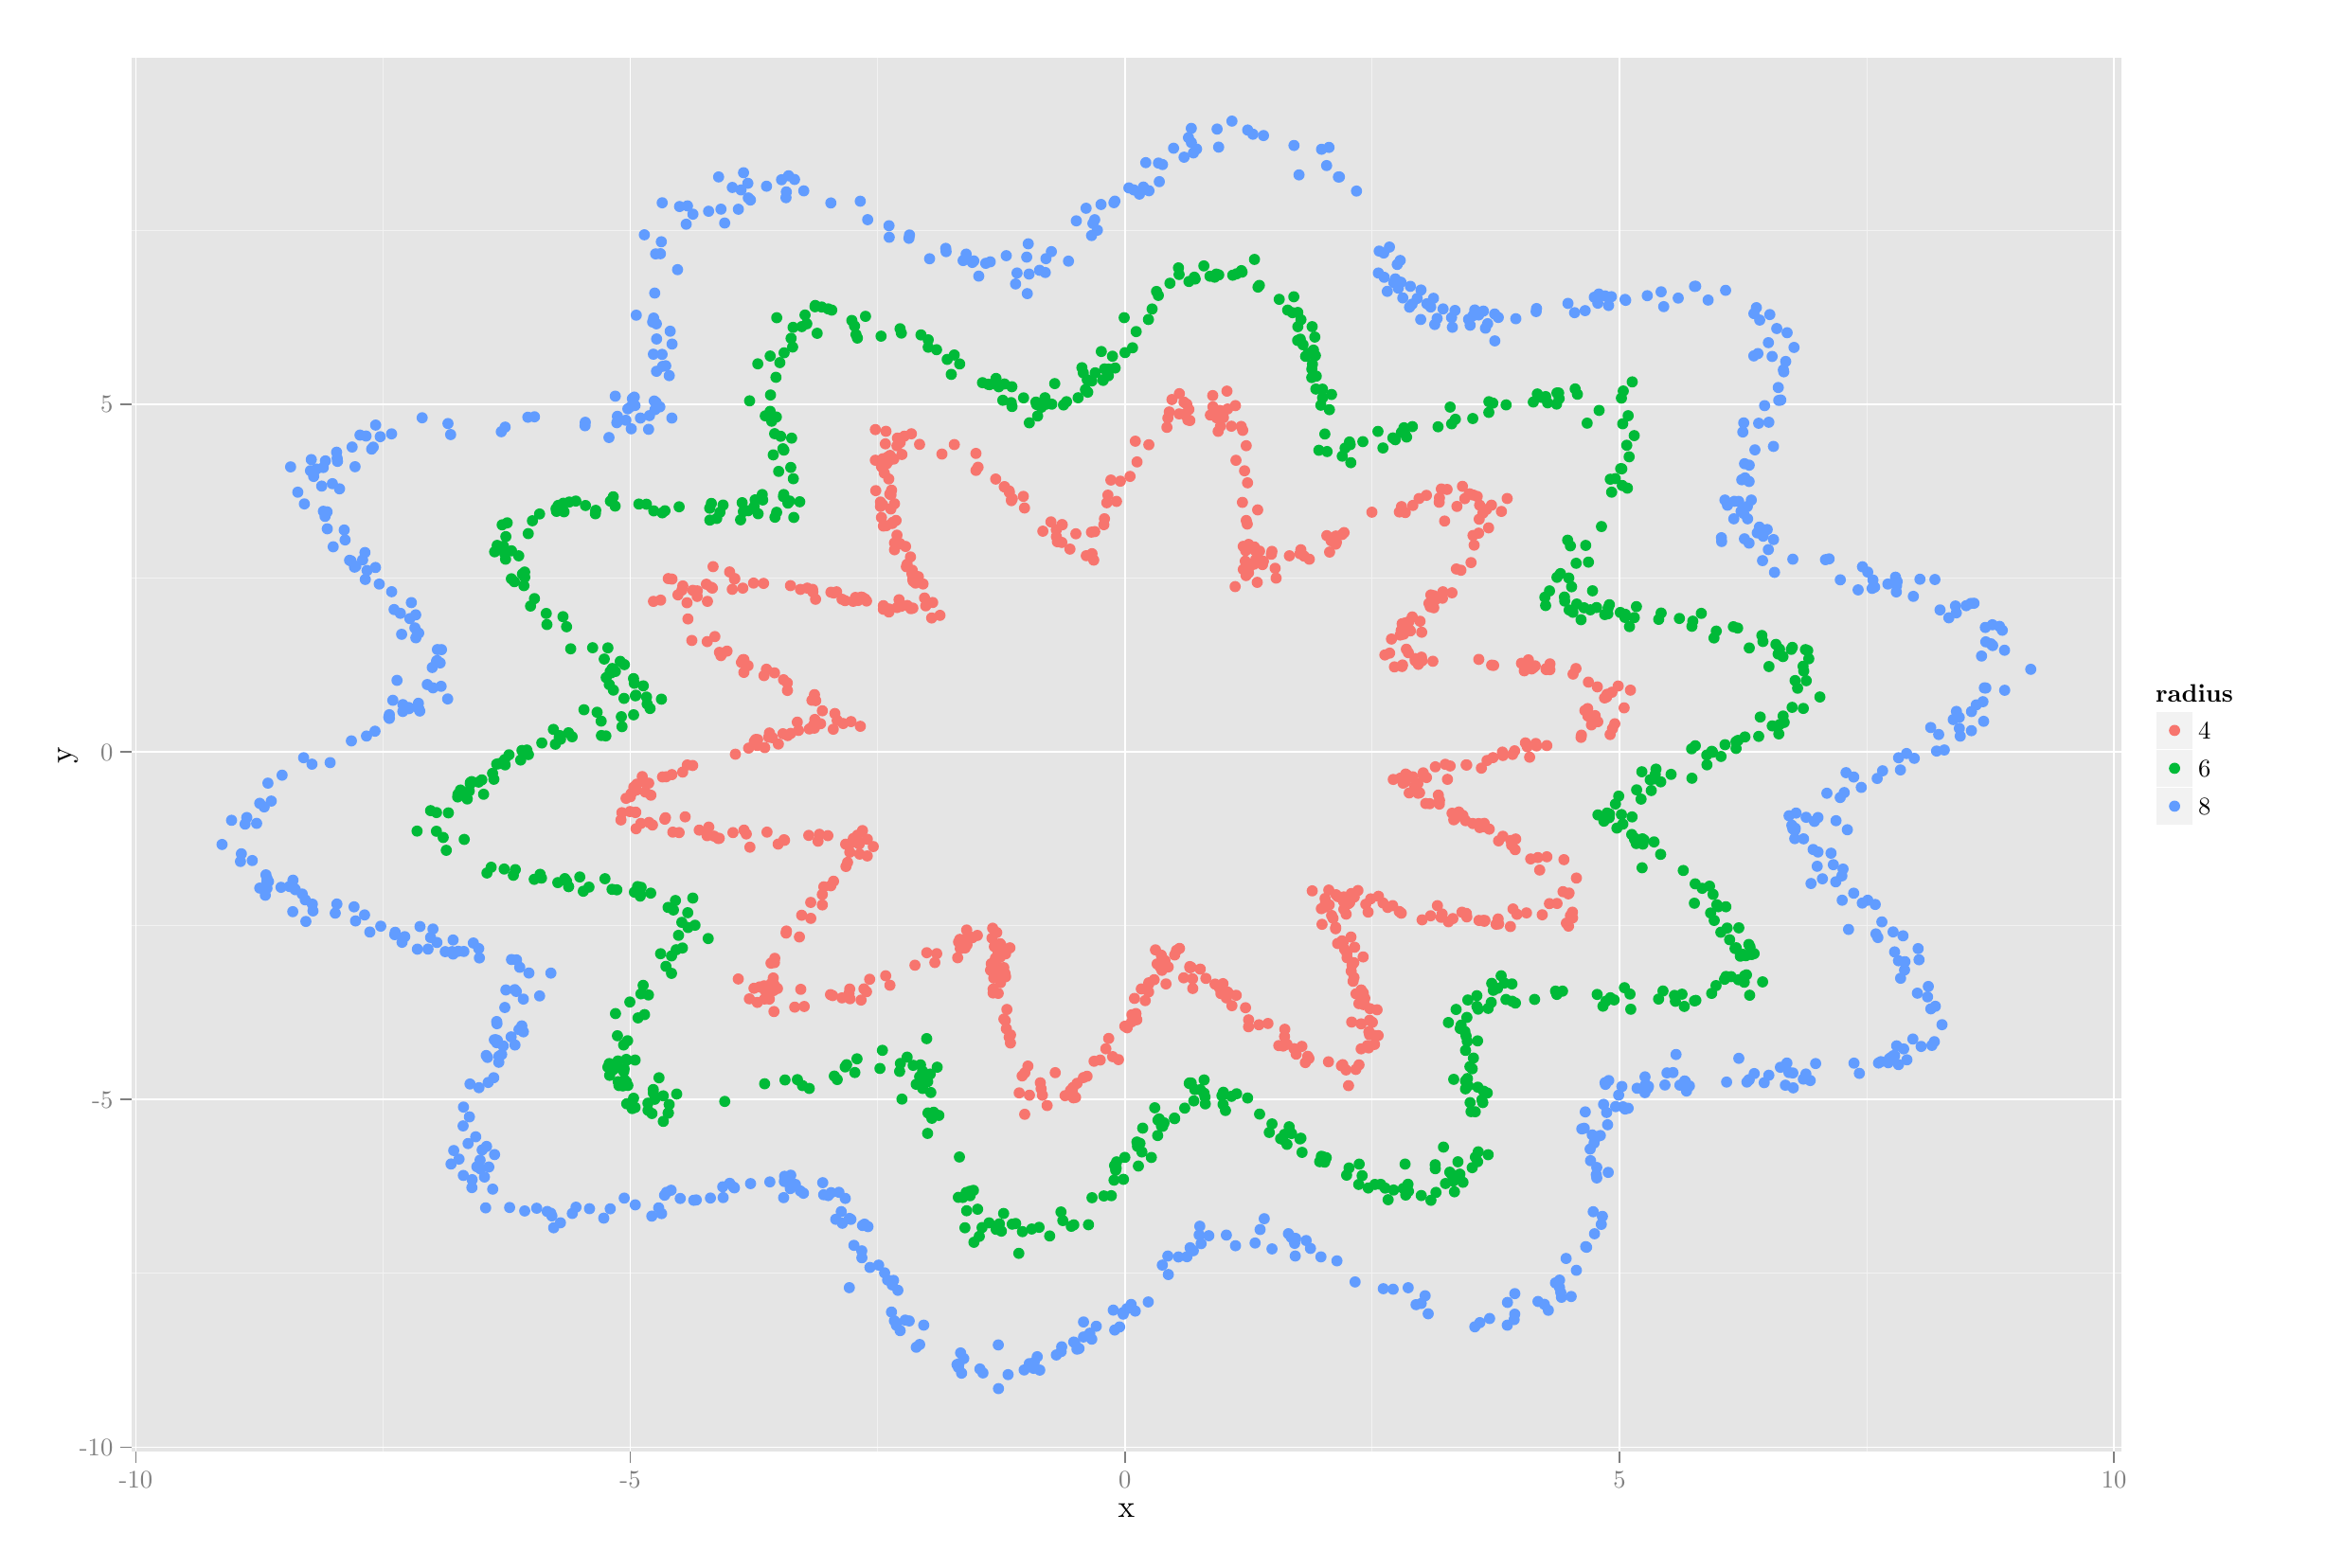
\begin{tikzpicture}[x=1pt,y=1pt]
\definecolor[named]{fillColor}{rgb}{1.00,1.00,1.00}
\path[use as bounding box,fill=fillColor,fill opacity=0.00] (0,0) rectangle (867.24,578.16);
\begin{scope}
\path[clip] (  0.00,  0.00) rectangle (867.24,578.16);
\definecolor[named]{drawColor}{rgb}{1.00,1.00,1.00}
\definecolor[named]{fillColor}{rgb}{1.00,1.00,1.00}

\path[draw=drawColor,line width= 0.6pt,line join=round,line cap=round,fill=fillColor] (  0.00, -0.00) rectangle (867.24,578.16);
\end{scope}
\begin{scope}
\path[clip] ( 40.22, 34.03) rectangle (799.33,566.12);
\definecolor[named]{fillColor}{rgb}{0.90,0.90,0.90}

\path[fill=fillColor] ( 40.22, 34.03) rectangle (799.33,566.12);
\definecolor[named]{drawColor}{rgb}{0.95,0.95,0.95}

\path[draw=drawColor,line width= 0.3pt,line join=round] ( 40.22,102.20) --
	(799.33,102.20);

\path[draw=drawColor,line width= 0.3pt,line join=round] ( 40.22,234.89) --
	(799.33,234.89);

\path[draw=drawColor,line width= 0.3pt,line join=round] ( 40.22,367.58) --
	(799.33,367.58);

\path[draw=drawColor,line width= 0.3pt,line join=round] ( 40.22,500.27) --
	(799.33,500.27);

\path[draw=drawColor,line width= 0.3pt,line join=round] (136.16, 34.03) --
	(136.16,566.12);

\path[draw=drawColor,line width= 0.3pt,line join=round] (324.85, 34.03) --
	(324.85,566.12);

\path[draw=drawColor,line width= 0.3pt,line join=round] (513.54, 34.03) --
	(513.54,566.12);

\path[draw=drawColor,line width= 0.3pt,line join=round] (702.23, 34.03) --
	(702.23,566.12);
\definecolor[named]{drawColor}{rgb}{1.00,1.00,1.00}

\path[draw=drawColor,line width= 0.6pt,line join=round] ( 40.22, 35.86) --
	(799.33, 35.86);

\path[draw=drawColor,line width= 0.6pt,line join=round] ( 40.22,168.55) --
	(799.33,168.55);

\path[draw=drawColor,line width= 0.6pt,line join=round] ( 40.22,301.24) --
	(799.33,301.24);

\path[draw=drawColor,line width= 0.6pt,line join=round] ( 40.22,433.93) --
	(799.33,433.93);

\path[draw=drawColor,line width= 0.6pt,line join=round] ( 41.81, 34.03) --
	( 41.81,566.12);

\path[draw=drawColor,line width= 0.6pt,line join=round] (230.50, 34.03) --
	(230.50,566.12);

\path[draw=drawColor,line width= 0.6pt,line join=round] (419.19, 34.03) --
	(419.19,566.12);

\path[draw=drawColor,line width= 0.6pt,line join=round] (607.88, 34.03) --
	(607.88,566.12);

\path[draw=drawColor,line width= 0.6pt,line join=round] (796.57, 34.03) --
	(796.57,566.12);
\definecolor[named]{fillColor}{rgb}{0.97,0.46,0.43}

\path[fill=fillColor] (275.63,302.64) circle (  2.13);

\path[fill=fillColor] (443.60,431.88) circle (  2.13);

\path[fill=fillColor] (476.52,371.28) circle (  2.13);

\path[fill=fillColor] (531.80,351.06) circle (  2.13);

\path[fill=fillColor] (330.41,388.37) circle (  2.13);

\path[fill=fillColor] (593.23,306.75) circle (  2.13);

\path[fill=fillColor] (506.69,245.83) circle (  2.13);

\path[fill=fillColor] (395.13,381.13) circle (  2.13);

\path[fill=fillColor] (329.60,414.35) circle (  2.13);

\path[fill=fillColor] (274.74,269.88) circle (  2.13);

\path[fill=fillColor] (368.91,209.20) circle (  2.13);

\path[fill=fillColor] (345.86,358.22) circle (  2.13);

\path[fill=fillColor] (559.63,299.03) circle (  2.13);

\path[fill=fillColor] (477.91,189.13) circle (  2.13);

\path[fill=fillColor] (345.47,352.31) circle (  2.13);

\path[fill=fillColor] (495.67,243.28) circle (  2.13);

\path[fill=fillColor] (507.38,208.89) circle (  2.13);

\path[fill=fillColor] (369.40,226.91) circle (  2.13);

\path[fill=fillColor] (526.18,392.55) circle (  2.13);

\path[fill=fillColor] (311.27,359.47) circle (  2.13);

\path[fill=fillColor] (331.02,412.97) circle (  2.13);

\path[fill=fillColor] (309.43,313.23) circle (  2.13);

\path[fill=fillColor] (256.79,271.36) circle (  2.13);

\path[fill=fillColor] (513.61,198.01) circle (  2.13);

\path[fill=fillColor] (552.13,399.23) circle (  2.13);

\path[fill=fillColor] (312.66,265.99) circle (  2.13);

\path[fill=fillColor] (324.15,400.91) circle (  2.13);

\path[fill=fillColor] (285.61,222.43) circle (  2.13);

\path[fill=fillColor] (468.47,372.86) circle (  2.13);

\path[fill=fillColor] (450.09,214.77) circle (  2.13);

\path[fill=fillColor] (329.49,399.62) circle (  2.13);

\path[fill=fillColor] (503.52,243.16) circle (  2.13);

\path[fill=fillColor] (549.63,296.21) circle (  2.13);

\path[fill=fillColor] (466.35,369.53) circle (  2.13);

\path[fill=fillColor] (373.97,195.56) circle (  2.13);

\path[fill=fillColor] (473.78,197.57) circle (  2.13);

\path[fill=fillColor] (375.33,226.43) circle (  2.13);

\path[fill=fillColor] (329.96,399.31) circle (  2.13);

\path[fill=fillColor] (532.36,337.36) circle (  2.13);

\path[fill=fillColor] (282.65,270.60) circle (  2.13);

\path[fill=fillColor] (318.00,262.21) circle (  2.13);

\path[fill=fillColor] (313.93,208.97) circle (  2.13);

\path[fill=fillColor] (285.30,202.12) circle (  2.13);

\path[fill=fillColor] (527.58,350.94) circle (  2.13);

\path[fill=fillColor] (475.29,377.74) circle (  2.13);

\path[fill=fillColor] (438.19,223.72) circle (  2.13);

\path[fill=fillColor] (536.70,335.80) circle (  2.13);

\path[fill=fillColor] (455.30,211.12) circle (  2.13);

\path[fill=fillColor] (273.83,336.43) circle (  2.13);

\path[fill=fillColor] (526.33,292.76) circle (  2.13);

\path[fill=fillColor] (338.14,369.85) circle (  2.13);

\path[fill=fillColor] (337.72,422.61) circle (  2.13);

\path[fill=fillColor] (549.65,238.24) circle (  2.13);

\path[fill=fillColor] (285.49,220.79) circle (  2.13);

\path[fill=fillColor] (535.84,238.66) circle (  2.13);

\path[fill=fillColor] (288.95,328.75) circle (  2.13);

\path[fill=fillColor] (407.43,183.15) circle (  2.13);

\path[fill=fillColor] (458.43,209.54) circle (  2.13);

\path[fill=fillColor] (373.03,199.27) circle (  2.13);

\path[fill=fillColor] (340.40,368.08) circle (  2.13);

\path[fill=fillColor] (540.23,239.35) circle (  2.13);

\path[fill=fillColor] (526.26,289.85) circle (  2.13);

\path[fill=fillColor] (286.98,304.21) circle (  2.13);

\path[fill=fillColor] (575.75,334.04) circle (  2.13);

\path[fill=fillColor] (326.80,395.51) circle (  2.13);

\path[fill=fillColor] (318.54,206.50) circle (  2.13);

\path[fill=fillColor] (375.05,192.35) circle (  2.13);

\path[fill=fillColor] (265.07,337.94) circle (  2.13);

\path[fill=fillColor] (554.37,390.02) circle (  2.13);

\path[fill=fillColor] (537.76,359.37) circle (  2.13);

\path[fill=fillColor] (603.13,323.19) circle (  2.13);

\path[fill=fillColor] (481.04,189.61) circle (  2.13);

\path[fill=fillColor] (504.43,243.26) circle (  2.13);

\path[fill=fillColor] (273.86,271.36) circle (  2.13);

\path[fill=fillColor] (508.11,248.31) circle (  2.13);

\path[fill=fillColor] (544.32,237.60) circle (  2.13);

\path[fill=fillColor] (568.09,263.90) circle (  2.13);

\path[fill=fillColor] (392.62,178.80) circle (  2.13);

\path[fill=fillColor] (329.15,354.60) circle (  2.13);

\path[fill=fillColor] (314.71,312.77) circle (  2.13);

\path[fill=fillColor] (558.21,271.73) circle (  2.13);

\path[fill=fillColor] (556.29,273.94) circle (  2.13);

\path[fill=fillColor] (529.96,335.98) circle (  2.13);

\path[fill=fillColor] (561.77,267.26) circle (  2.13);

\path[fill=fillColor] (433.32,217.84) circle (  2.13);

\path[fill=fillColor] (551.94,273.87) circle (  2.13);

\path[fill=fillColor] (430.36,214.27) circle (  2.13);

\path[fill=fillColor] (494.15,241.37) circle (  2.13);

\path[fill=fillColor] (537.15,360.80) circle (  2.13);

\path[fill=fillColor] (497.87,381.80) circle (  2.13);

\path[fill=fillColor] (254.28,296.02) circle (  2.13);

\path[fill=fillColor] (333.02,359.29) circle (  2.13);

\path[fill=fillColor] (277.52,365.63) circle (  2.13);

\path[fill=fillColor] (598.28,314.41) circle (  2.13);

\path[fill=fillColor] (501.80,181.41) circle (  2.13);

\path[fill=fillColor] (423.18,419.78) circle (  2.13);

\path[fill=fillColor] (428.33,418.43) circle (  2.13);

\path[fill=fillColor] (300.03,363.25) circle (  2.13);

\path[fill=fillColor] (332.25,356.29) circle (  2.13);

\path[fill=fillColor] (451.82,429.76) circle (  2.13);

\path[fill=fillColor] (574.39,332.87) circle (  2.13);

\path[fill=fillColor] (338.05,370.55) circle (  2.13);

\path[fill=fillColor] (404.75,177.43) circle (  2.13);

\path[fill=fillColor] (356.39,226.14) circle (  2.13);

\path[fill=fillColor] (555.21,295.01) circle (  2.13);

\path[fill=fillColor] (607.41,326.36) circle (  2.13);

\path[fill=fillColor] (398.23,378.60) circle (  2.13);

\path[fill=fillColor] (557.96,386.71) circle (  2.13);

\path[fill=fillColor] (327.41,407.62) circle (  2.13);

\path[fill=fillColor] (515.94,246.12) circle (  2.13);

\path[fill=fillColor] (499.63,234.26) circle (  2.13);

\path[fill=fillColor] (369.90,405.33) circle (  2.13);

\path[fill=fillColor] (303.74,246.78) circle (  2.13);

\path[fill=fillColor] (358.97,227.61) circle (  2.13);

\path[fill=fillColor] (238.94,273.31) circle (  2.13);

\path[fill=fillColor] (480.11,192.58) circle (  2.13);

\path[fill=fillColor] (524.92,333.80) circle (  2.13);

\path[fill=fillColor] (327.05,387.40) circle (  2.13);

\path[fill=fillColor] (315.52,358.67) circle (  2.13);

\path[fill=fillColor] (276.12,264.84) circle (  2.13);

\path[fill=fillColor] (320.62,209.70) circle (  2.13);

\path[fill=fillColor] (551.26,373.46) circle (  2.13);

\path[fill=fillColor] (469.94,374.52) circle (  2.13);

\path[fill=fillColor] (369.81,222.51) circle (  2.13);

\path[fill=fillColor] (362.36,415.12) circle (  2.13);

\path[fill=fillColor] (319.05,360.17) circle (  2.13);

\path[fill=fillColor] (455.83,208.96) circle (  2.13);

\path[fill=fillColor] (510.23,204.78) circle (  2.13);

\path[fill=fillColor] (330.16,401.09) circle (  2.13);

\path[fill=fillColor] (237.51,289.28) circle (  2.13);

\path[fill=fillColor] (338.27,367.03) circle (  2.13);

\path[fill=fillColor] (465.44,368.50) circle (  2.13);

\path[fill=fillColor] (539.47,360.21) circle (  2.13);

\path[fill=fillColor] (419.18,196.52) circle (  2.13);

\path[fill=fillColor] (283.54,206.88) circle (  2.13);

\path[fill=fillColor] (317.41,359.00) circle (  2.13);

\path[fill=fillColor] (307.69,208.20) circle (  2.13);

\path[fill=fillColor] (414.52,184.91) circle (  2.13);

\path[fill=fillColor] (561.60,237.46) circle (  2.13);

\path[fill=fillColor] (316.71,267.09) circle (  2.13);

\path[fill=fillColor] (301.24,320.77) circle (  2.13);

\path[fill=fillColor] (486.33,378.36) circle (  2.13);

\path[fill=fillColor] (354.12,418.50) circle (  2.13);

\path[fill=fillColor] (284.17,220.59) circle (  2.13);

\path[fill=fillColor] (284.22,212.78) circle (  2.13);

\path[fill=fillColor] (581.35,332.60) circle (  2.13);

\path[fill=fillColor] (560.82,235.44) circle (  2.13);

\path[fill=fillColor] (308.03,251.85) circle (  2.13);

\path[fill=fillColor] (524.65,239.67) circle (  2.13);

\path[fill=fillColor] (573.14,336.33) circle (  2.13);

\path[fill=fillColor] (588.46,234.72) circle (  2.13);

\path[fill=fillColor] (529.92,336.83) circle (  2.13);

\path[fill=fillColor] (465.49,418.06) circle (  2.13);

\path[fill=fillColor] (539.17,281.29) circle (  2.13);

\path[fill=fillColor] (290.45,324.66) circle (  2.13);

\path[fill=fillColor] (597.20,311.51) circle (  2.13);

\path[fill=fillColor] (505.45,230.56) circle (  2.13);

\path[fill=fillColor] (509.32,197.42) circle (  2.13);

\path[fill=fillColor] (368.48,230.14) circle (  2.13);

\path[fill=fillColor] (464.04,396.43) circle (  2.13);

\path[fill=fillColor] (563.42,269.02) circle (  2.13);

\path[fill=fillColor] (253.96,343.74) circle (  2.13);

\path[fill=fillColor] (327.80,418.77) circle (  2.13);

\path[fill=fillColor] (371.61,228.01) circle (  2.13);

\path[fill=fillColor] (542.64,236.37) circle (  2.13);

\path[fill=fillColor] (503.89,224.35) circle (  2.13);

\path[fill=fillColor] (268.38,369.88) circle (  2.13);

\path[fill=fillColor] (285.51,331.37) circle (  2.13);

\path[fill=fillColor] (395.29,387.90) circle (  2.13);

\path[fill=fillColor] (375.56,193.22) circle (  2.13);

\path[fill=fillColor] (496.87,182.95) circle (  2.13);

\path[fill=fillColor] (468.57,379.42) circle (  2.13);

\path[fill=fillColor] (508.48,205.15) circle (  2.13);

\path[fill=fillColor] (273.42,363.71) circle (  2.13);

\path[fill=fillColor] (284.72,210.15) circle (  2.13);

\path[fill=fillColor] (594.70,316.99) circle (  2.13);

\path[fill=fillColor] (568.79,239.23) circle (  2.13);

\path[fill=fillColor] (308.13,361.85) circle (  2.13);

\path[fill=fillColor] (281.50,330.32) circle (  2.13);

\path[fill=fillColor] (347.40,224.22) circle (  2.13);

\path[fill=fillColor] (319.63,210.77) circle (  2.13);

\path[fill=fillColor] (252.12,358.12) circle (  2.13);

\path[fill=fillColor] (300.76,323.07) circle (  2.13);

\path[fill=fillColor] (499.59,233.72) circle (  2.13);

\path[fill=fillColor] (573.62,299.18) circle (  2.13);

\path[fill=fillColor] (454.78,423.54) circle (  2.13);

\path[fill=fillColor] (605.24,310.09) circle (  2.13);

\path[fill=fillColor] (380.45,398.72) circle (  2.13);

\path[fill=fillColor] (294.20,312.56) circle (  2.13);

\path[fill=fillColor] (333.80,356.76) circle (  2.13);

\path[fill=fillColor] (443.96,219.28) circle (  2.13);

\path[fill=fillColor] (541.18,389.31) circle (  2.13);

\path[fill=fillColor] (549.20,274.94) circle (  2.13);

\path[fill=fillColor] (368.91,210.67) circle (  2.13);

\path[fill=fillColor] (279.06,305.91) circle (  2.13);

\path[fill=fillColor] (438.89,225.45) circle (  2.13);

\path[fill=fillColor] (291.60,364.66) circle (  2.13);

\path[fill=fillColor] (506.85,226.67) circle (  2.13);

\path[fill=fillColor] (250.47,293.51) circle (  2.13);

\path[fill=fillColor] (456.26,429.51) circle (  2.13);

\path[fill=fillColor] (330.60,388.80) circle (  2.13);

\path[fill=fillColor] (463.56,425.41) circle (  2.13);

\path[fill=fillColor] (441.97,430.05) circle (  2.13);

\path[fill=fillColor] (466.41,380.40) circle (  2.13);

\path[fill=fillColor] (395.17,387.91) circle (  2.13);

\path[fill=fillColor] (525.64,349.57) circle (  2.13);

\path[fill=fillColor] (252.24,296.21) circle (  2.13);

\path[fill=fillColor] (298.02,363.71) circle (  2.13);

\path[fill=fillColor] (283.57,308.44) circle (  2.13);

\path[fill=fillColor] (260.44,272.52) circle (  2.13);

\path[fill=fillColor] (371.56,222.82) circle (  2.13);

\path[fill=fillColor] (230.51,284.11) circle (  2.13);

\path[fill=fillColor] (235.04,291.80) circle (  2.13);

\path[fill=fillColor] (319.07,271.19) circle (  2.13);

\path[fill=fillColor] (554.54,395.36) circle (  2.13);

\path[fill=fillColor] (455.37,431.54) circle (  2.13);

\path[fill=fillColor] (421.86,200.92) circle (  2.13);

\path[fill=fillColor] (540.53,362.30) circle (  2.13);

\path[fill=fillColor] (506.25,213.67) circle (  2.13);

\path[fill=fillColor] (505.54,217.54) circle (  2.13);

\path[fill=fillColor] (314.32,207.01) circle (  2.13);

\path[fill=fillColor] (262.42,269.07) circle (  2.13);

\path[fill=fillColor] (546.61,278.28) circle (  2.13);

\path[fill=fillColor] (278.89,303.66) circle (  2.13);

\path[fill=fillColor] (387.23,172.66) circle (  2.13);

\path[fill=fillColor] (417.47,404.52) circle (  2.13);

\path[fill=fillColor] (425.46,210.76) circle (  2.13);

\path[fill=fillColor] (282.43,332.76) circle (  2.13);

\path[fill=fillColor] (498.07,238.78) circle (  2.13);

\path[fill=fillColor] (326.29,410.20) circle (  2.13);

\path[fill=fillColor] (435.23,425.07) circle (  2.13);

\path[fill=fillColor] (270.23,367.19) circle (  2.13);

\path[fill=fillColor] (584.07,243.37) circle (  2.13);

\path[fill=fillColor] (358.83,233.23) circle (  2.13);

\path[fill=fillColor] (442.81,433.88) circle (  2.13);

\path[fill=fillColor] (232.56,278.21) circle (  2.13);

\path[fill=fillColor] (312.43,358.93) circle (  2.13);

\path[fill=fillColor] (295.87,238.87) circle (  2.13);

\path[fill=fillColor] (311.26,207.34) circle (  2.13);

\path[fill=fillColor] (500.47,245.96) circle (  2.13);

\path[fill=fillColor] (531.63,285.61) circle (  2.13);

\path[fill=fillColor] (390.98,388.99) circle (  2.13);

\path[fill=fillColor] (403.38,176.92) circle (  2.13);

\path[fill=fillColor] (327.02,355.66) circle (  2.13);

\path[fill=fillColor] (535.70,356.60) circle (  2.13);

\path[fill=fillColor] (526.60,291.89) circle (  2.13);

\path[fill=fillColor] (407.69,385.28) circle (  2.13);

\path[fill=fillColor] (428.30,213.09) circle (  2.13);

\path[fill=fillColor] (522.03,333.65) circle (  2.13);

\path[fill=fillColor] (407.31,374.39) circle (  2.13);

\path[fill=fillColor] (375.90,397.10) circle (  2.13);

\path[fill=fillColor] (325.94,394.88) circle (  2.13);

\path[fill=fillColor] (524.73,394.82) circle (  2.13);

\path[fill=fillColor] (452.70,437.19) circle (  2.13);

\path[fill=fillColor] (532.56,335.95) circle (  2.13);

\path[fill=fillColor] (230.77,285.26) circle (  2.13);

\path[fill=fillColor] (262.75,345.22) circle (  2.13);

\path[fill=fillColor] (339.09,219.81) circle (  2.13);

\path[fill=fillColor] (355.39,222.65) circle (  2.13);

\path[fill=fillColor] (464.16,423.93) circle (  2.13);

\path[fill=fillColor] (382.78,170.19) circle (  2.13);

\path[fill=fillColor] (567.27,241.26) circle (  2.13);

\path[fill=fillColor] (581.18,243.31) circle (  2.13);

\path[fill=fillColor] (562.86,392.98) circle (  2.13);

\path[fill=fillColor] (460.03,204.36) circle (  2.13);

\path[fill=fillColor] (471.71,372.69) circle (  2.13);

\path[fill=fillColor] (521.35,242.56) circle (  2.13);

\path[fill=fillColor] (504.96,243.70) circle (  2.13);

\path[fill=fillColor] (475.07,376.64) circle (  2.13);

\path[fill=fillColor] (514.44,189.59) circle (  2.13);

\path[fill=fillColor] (511.99,240.08) circle (  2.13);

\path[fill=fillColor] (433.07,223.64) circle (  2.13);

\path[fill=fillColor] (284.69,306.64) circle (  2.13);

\path[fill=fillColor] (554.58,272.33) circle (  2.13);

\path[fill=fillColor] (572.73,303.17) circle (  2.13);

\path[fill=fillColor] (273.82,331.55) circle (  2.13);

\path[fill=fillColor] (327.93,215.77) circle (  2.13);

\path[fill=fillColor] (261.37,364.03) circle (  2.13);

\path[fill=fillColor] (542.27,290.74) circle (  2.13);

\path[fill=fillColor] (497.15,242.83) circle (  2.13);

\path[fill=fillColor] (572.02,304.64) circle (  2.13);

\path[fill=fillColor] (300.14,362.26) circle (  2.13);

\path[fill=fillColor] (561.80,235.56) circle (  2.13);

\path[fill=fillColor] (270.35,367.35) circle (  2.13);

\path[fill=fillColor] (461.57,412.49) circle (  2.13);

\path[fill=fillColor] (559.89,334.22) circle (  2.13);

\path[fill=fillColor] (580.18,303.63) circle (  2.13);

\path[fill=fillColor] (443.22,427.90) circle (  2.13);

\path[fill=fillColor] (455.89,211.56) circle (  2.13);

\path[fill=fillColor] (556.32,236.56) circle (  2.13);

\path[fill=fillColor] (484.55,185.87) circle (  2.13);

\path[fill=fillColor] (544.67,275.28) circle (  2.13);

\path[fill=fillColor] (340.85,418.57) circle (  2.13);

\path[fill=fillColor] (232.69,271.89) circle (  2.13);

\path[fill=fillColor] (387.89,385.44) circle (  2.13);

\path[fill=fillColor] (358.21,226.37) circle (  2.13);

\path[fill=fillColor] (264.42,268.23) circle (  2.13);

\path[fill=fillColor] (242.78,291.66) circle (  2.13);

\path[fill=fillColor] (318.26,310.98) circle (  2.13);

\path[fill=fillColor] (578.43,239.04) circle (  2.13);

\path[fill=fillColor] (495.55,242.01) circle (  2.13);

\path[fill=fillColor] (524.97,350.12) circle (  2.13);

\path[fill=fillColor] (285.18,210.15) circle (  2.13);

\path[fill=fillColor] (246.39,367.16) circle (  2.13);

\path[fill=fillColor] (567.11,300.25) circle (  2.13);

\path[fill=fillColor] (524.62,347.59) circle (  2.13);

\path[fill=fillColor] (426.95,206.29) circle (  2.13);

\path[fill=fillColor] (570.51,335.03) circle (  2.13);

\path[fill=fillColor] (370.65,217.79) circle (  2.13);

\path[fill=fillColor] (529.68,286.85) circle (  2.13);

\path[fill=fillColor] (598.62,315.04) circle (  2.13);

\path[fill=fillColor] (455.67,425.49) circle (  2.13);

\path[fill=fillColor] (300.89,313.59) circle (  2.13);

\path[fill=fillColor] (512.54,198.80) circle (  2.13);

\path[fill=fillColor] (515.82,192.97) circle (  2.13);

\path[fill=fillColor] (399.27,170.83) circle (  2.13);

\path[fill=fillColor] (271.69,214.55) circle (  2.13);

\path[fill=fillColor] (605.01,323.98) circle (  2.13);

\path[fill=fillColor] (531.16,334.62) circle (  2.13);

\path[fill=fillColor] (452.79,432.89) circle (  2.13);

\path[fill=fillColor] (304.33,249.72) circle (  2.13);

\path[fill=fillColor] (575.98,304.43) circle (  2.13);

\path[fill=fillColor] (453.58,212.60) circle (  2.13);

\path[fill=fillColor] (303.76,242.81) circle (  2.13);

\path[fill=fillColor] (466.83,371.98) circle (  2.13);

\path[fill=fillColor] (528.83,352.72) circle (  2.13);

\path[fill=fillColor] (278.34,305.95) circle (  2.13);

\path[fill=fillColor] (502.31,181.87) circle (  2.13);

\path[fill=fillColor] (423.74,199.00) circle (  2.13);

\path[fill=fillColor] (332.42,420.96) circle (  2.13);

\path[fill=fillColor] (439.91,430.20) circle (  2.13);

\path[fill=fillColor] (440.03,226.21) circle (  2.13);

\path[fill=fillColor] (306.87,208.59) circle (  2.13);

\path[fill=fillColor] (556.62,272.58) circle (  2.13);

\path[fill=fillColor] (539.11,396.49) circle (  2.13);

\path[fill=fillColor] (563.23,301.13) circle (  2.13);

\path[fill=fillColor] (250.17,362.93) circle (  2.13);

\path[fill=fillColor] (456.47,430.11) circle (  2.13);

\path[fill=fillColor] (328.25,411.15) circle (  2.13);

\path[fill=fillColor] (393.43,381.41) circle (  2.13);

\path[fill=fillColor] (333.45,419.25) circle (  2.13);

\path[fill=fillColor] (575.23,333.48) circle (  2.13);

\path[fill=fillColor] (323.19,265.08) circle (  2.13);

\path[fill=fillColor] (328.04,423.56) circle (  2.13);

\path[fill=fillColor] (526.59,340.39) circle (  2.13);

\path[fill=fillColor] (317.82,266.02) circle (  2.13);

\path[fill=fillColor] (295.53,210.60) circle (  2.13);

\path[fill=fillColor] (259.83,343.30) circle (  2.13);

\path[fill=fillColor] (445.08,210.92) circle (  2.13);

\path[fill=fillColor] (539.24,282.72) circle (  2.13);

\path[fill=fillColor] (312.77,257.49) circle (  2.13);

\path[fill=fillColor] (399.38,173.12) circle (  2.13);

\path[fill=fillColor] (244.97,367.35) circle (  2.13);

\path[fill=fillColor] (290.54,307.43) circle (  2.13);

\path[fill=fillColor] (599.62,312.73) circle (  2.13);

\path[fill=fillColor] (444.41,219.04) circle (  2.13);

\path[fill=fillColor] (505.57,247.15) circle (  2.13);

\path[fill=fillColor] (323.99,424.21) circle (  2.13);

\path[fill=fillColor] (497.30,377.47) circle (  2.13);

\path[fill=fillColor] (320.63,358.80) circle (  2.13);

\path[fill=fillColor] (302.64,269.76) circle (  2.13);

\path[fill=fillColor] (512.33,194.21) circle (  2.13);

\path[fill=fillColor] (318.59,360.29) circle (  2.13);

\path[fill=fillColor] (554.22,336.51) circle (  2.13);

\path[fill=fillColor] (444.01,218.83) circle (  2.13);

\path[fill=fillColor] (373.29,402.39) circle (  2.13);

\path[fill=fillColor] (534.24,399.12) circle (  2.13);

\path[fill=fillColor] (502.04,229.09) circle (  2.13);

\path[fill=fillColor] (456.61,212.77) circle (  2.13);

\path[fill=fillColor] (550.49,399.58) circle (  2.13);

\path[fill=fillColor] (506.53,220.76) circle (  2.13);

\path[fill=fillColor] (489.56,374.74) circle (  2.13);

\path[fill=fillColor] (302.11,267.14) circle (  2.13);

\path[fill=fillColor] (411.17,387.92) circle (  2.13);

\path[fill=fillColor] (359.35,231.17) circle (  2.13);

\path[fill=fillColor] (289.33,267.45) circle (  2.13);

\path[fill=fillColor] (291.68,308.27) circle (  2.13);

\path[fill=fillColor] (289.93,232.08) circle (  2.13);

\path[fill=fillColor] (370.01,221.49) circle (  2.13);

\path[fill=fillColor] (510.39,205.21) circle (  2.13);

\path[fill=fillColor] (521.59,290.70) circle (  2.13);

\path[fill=fillColor] (537.64,295.52) circle (  2.13);

\path[fill=fillColor] (513.44,392.69) circle (  2.13);

\path[fill=fillColor] (512.33,194.47) circle (  2.13);

\path[fill=fillColor] (612.09,324.77) circle (  2.13);

\path[fill=fillColor] (314.20,210.71) circle (  2.13);

\path[fill=fillColor] (404.47,376.08) circle (  2.13);

\path[fill=fillColor] (236.25,285.90) circle (  2.13);

\path[fill=fillColor] (288.72,308.13) circle (  2.13);

\path[fill=fillColor] (518.39,338.20) circle (  2.13);

\path[fill=fillColor] (281.33,365.52) circle (  2.13);

\path[fill=fillColor] (434.49,221.53) circle (  2.13);

\path[fill=fillColor] (422.85,207.14) circle (  2.13);

\path[fill=fillColor] (286.90,266.03) circle (  2.13);

\path[fill=fillColor] (326.83,413.09) circle (  2.13);

\path[fill=fillColor] (586.70,260.08) circle (  2.13);

\path[fill=fillColor] (285.03,214.92) circle (  2.13);

\path[fill=fillColor] (421.80,198.21) circle (  2.13);

\path[fill=fillColor] (242.07,359.13) circle (  2.13);

\path[fill=fillColor] (348.64,353.32) circle (  2.13);

\path[fill=fillColor] (456.28,209.61) circle (  2.13);

\path[fill=fillColor] (368.74,233.92) circle (  2.13);

\path[fill=fillColor] (337.55,355.86) circle (  2.13);

\path[fill=fillColor] (502.73,241.13) circle (  2.13);

\path[fill=fillColor] (376.00,397.72) circle (  2.13);

\path[fill=fillColor] (436.12,430.94) circle (  2.13);

\path[fill=fillColor] (539.21,398.15) circle (  2.13);

\path[fill=fillColor] (543.28,295.83) circle (  2.13);

\path[fill=fillColor] (428.25,209.60) circle (  2.13);

\path[fill=fillColor] (332.22,418.01) circle (  2.13);

\path[fill=fillColor] (281.70,206.91) circle (  2.13);

\path[fill=fillColor] (472.04,373.96) circle (  2.13);

\path[fill=fillColor] (421.16,406.35) circle (  2.13);

\path[fill=fillColor] (517.68,243.57) circle (  2.13);

\path[fill=fillColor] (329.10,405.37) circle (  2.13);

\path[fill=fillColor] (527.67,285.56) circle (  2.13);

\path[fill=fillColor] (329.20,355.77) circle (  2.13);

\path[fill=fillColor] (296.85,204.05) circle (  2.13);

\path[fill=fillColor] (278.97,205.61) circle (  2.13);

\path[fill=fillColor] (373.69,215.41) circle (  2.13);

\path[fill=fillColor] (489.41,184.21) circle (  2.13);

\path[fill=fillColor] (539.93,401.55) circle (  2.13);

\path[fill=fillColor] (375.53,190.11) circle (  2.13);

\path[fill=fillColor] (264.00,268.16) circle (  2.13);

\path[fill=fillColor] (495.90,242.91) circle (  2.13);

\path[fill=fillColor] (515.41,202.80) circle (  2.13);

\path[fill=fillColor] (342.18,365.29) circle (  2.13);

\path[fill=fillColor] (285.39,212.27) circle (  2.13);

\path[fill=fillColor] (371.98,227.36) circle (  2.13);

\path[fill=fillColor] (571.57,332.14) circle (  2.13);

\path[fill=fillColor] (299.79,320.91) circle (  2.13);

\path[fill=fillColor] (576.25,303.49) circle (  2.13);

\path[fill=fillColor] (557.37,297.94) circle (  2.13);

\path[fill=fillColor] (554.15,384.69) circle (  2.13);

\path[fill=fillColor] (275.41,334.11) circle (  2.13);

\path[fill=fillColor] (430.86,225.66) circle (  2.13);

\path[fill=fillColor] (362.90,231.17) circle (  2.13);

\path[fill=fillColor] (506.60,215.12) circle (  2.13);

\path[fill=fillColor] (337.95,369.16) circle (  2.13);

\path[fill=fillColor] (447.95,218.31) circle (  2.13);

\path[fill=fillColor] (376.24,397.80) circle (  2.13);

\path[fill=fillColor] (512.54,193.25) circle (  2.13);

\path[fill=fillColor] (588.66,247.35) circle (  2.13);

\path[fill=fillColor] (507.30,180.03) circle (  2.13);

\path[fill=fillColor] (596.05,327.84) circle (  2.13);

\path[fill=fillColor] (441.63,214.99) circle (  2.13);

\path[fill=fillColor] (374.17,202.92) circle (  2.13);

\path[fill=fillColor] (299.35,237.68) circle (  2.13);

\path[fill=fillColor] (589.94,240.04) circle (  2.13);

\path[fill=fillColor] (466.38,196.32) circle (  2.13);

\path[fill=fillColor] (532.58,237.11) circle (  2.13);

\path[fill=fillColor] (544.02,277.80) circle (  2.13);

\path[fill=fillColor] (445.00,214.63) circle (  2.13);

\path[fill=fillColor] (543.99,361.93) circle (  2.13);

\path[fill=fillColor] (500.36,228.09) circle (  2.13);

\path[fill=fillColor] (435.59,428.61) circle (  2.13);

\path[fill=fillColor] (298.81,309.96) circle (  2.13);

\path[fill=fillColor] (307.03,362.15) circle (  2.13);

\path[fill=fillColor] (331.29,380.96) circle (  2.13);

\path[fill=fillColor] (387.72,170.20) circle (  2.13);

\path[fill=fillColor] (465.88,388.16) circle (  2.13);

\path[fill=fillColor] (548.16,276.96) circle (  2.13);

\path[fill=fillColor] (293.22,203.80) circle (  2.13);

\path[fill=fillColor] (412.72,399.19) circle (  2.13);

\path[fill=fillColor] (261.80,363.72) circle (  2.13);

\path[fill=fillColor] (441.74,434.69) circle (  2.13);

\path[fill=fillColor] (389.52,166.25) circle (  2.13);

\path[fill=fillColor] (524.27,291.17) circle (  2.13);

\path[fill=fillColor] (380.90,394.29) circle (  2.13);

\path[fill=fillColor] (469.45,374.07) circle (  2.13);

\path[fill=fillColor] (527.04,292.18) circle (  2.13);

\path[fill=fillColor] (480.21,195.35) circle (  2.13);

\path[fill=fillColor] (531.43,397.91) circle (  2.13);

\path[fill=fillColor] (380.97,162.91) circle (  2.13);

\path[fill=fillColor] (566.74,265.60) circle (  2.13);

\path[fill=fillColor] (602.99,322.17) circle (  2.13);

\path[fill=fillColor] (469.86,393.57) circle (  2.13);

\path[fill=fillColor] (599.45,326.02) circle (  2.13);

\path[fill=fillColor] (479.56,188.95) circle (  2.13);

\path[fill=fillColor] (303.07,311.96) circle (  2.13);

\path[fill=fillColor] (523.91,392.77) circle (  2.13);

\path[fill=fillColor] (334.12,414.71) circle (  2.13);

\path[fill=fillColor] (428.22,212.50) circle (  2.13);

\path[fill=fillColor] (539.85,238.07) circle (  2.13);

\path[fill=fillColor] (256.01,360.54) circle (  2.13);

\path[fill=fillColor] (527.34,339.08) circle (  2.13);

\path[fill=fillColor] (326.24,395.56) circle (  2.13);

\path[fill=fillColor] (537.04,356.21) circle (  2.13);

\path[fill=fillColor] (535.93,361.11) circle (  2.13);

\path[fill=fillColor] (294.66,309.41) circle (  2.13);

\path[fill=fillColor] (465.99,403.90) circle (  2.13);

\path[fill=fillColor] (305.86,269.25) circle (  2.13);

\path[fill=fillColor] (586.35,247.87) circle (  2.13);

\path[fill=fillColor] (336.18,357.08) circle (  2.13);

\path[fill=fillColor] (416.74,183.77) circle (  2.13);

\path[fill=fillColor] (338.30,356.08) circle (  2.13);

\path[fill=fillColor] (393.03,385.94) circle (  2.13);

\path[fill=fillColor] (252.47,351.95) circle (  2.13);

\path[fill=fillColor] (606.11,311.95) circle (  2.13);

\path[fill=fillColor] (555.95,236.90) circle (  2.13);

\path[fill=fillColor] (511.68,189.09) circle (  2.13);

\path[fill=fillColor] (498.60,237.72) circle (  2.13);

\path[fill=fillColor] (567.89,301.61) circle (  2.13);

\path[fill=fillColor] (466.39,198.95) circle (  2.13);

\path[fill=fillColor] (547.41,370.53) circle (  2.13);

\path[fill=fillColor] (434.88,212.66) circle (  2.13);

\path[fill=fillColor] (524.22,345.80) circle (  2.13);

\path[fill=fillColor] (487.57,375.93) circle (  2.13);

\path[fill=fillColor] (512.68,203.23) circle (  2.13);

\path[fill=fillColor] (486.73,188.83) circle (  2.13);

\path[fill=fillColor] (503.97,222.66) circle (  2.13);

\path[fill=fillColor] (327.03,357.01) circle (  2.13);

\path[fill=fillColor] (470.57,377.82) circle (  2.13);

\path[fill=fillColor] (290.38,327.54) circle (  2.13);

\path[fill=fillColor] (579.95,332.62) circle (  2.13);

\path[fill=fillColor] (336.11,372.82) circle (  2.13);

\path[fill=fillColor] (559.13,334.32) circle (  2.13);

\path[fill=fillColor] (382.19,181.31) circle (  2.13);

\path[fill=fillColor] (534.26,291.42) circle (  2.13);

\path[fill=fillColor] (510.09,222.96) circle (  2.13);

\path[fill=fillColor] (326.59,409.76) circle (  2.13);

\path[fill=fillColor] (423.83,411.87) circle (  2.13);

\path[fill=fillColor] (373.56,198.66) circle (  2.13);

\path[fill=fillColor] (465.50,389.51) circle (  2.13);

\path[fill=fillColor] (581.38,334.80) circle (  2.13);

\path[fill=fillColor] (411.40,390.17) circle (  2.13);

\path[fill=fillColor] (360.96,230.27) circle (  2.13);

\path[fill=fillColor] (331.89,389.53) circle (  2.13);

\path[fill=fillColor] (411.93,187.91) circle (  2.13);

\path[fill=fillColor] (393.06,383.35) circle (  2.13);

\path[fill=fillColor] (232.45,278.08) circle (  2.13);

\path[fill=fillColor] (277.82,305.24) circle (  2.13);

\path[fill=fillColor] (227.28,278.01) circle (  2.13);

\path[fill=fillColor] (277.68,211.00) circle (  2.13);

\path[fill=fillColor] (499.63,380.51) circle (  2.13);

\path[fill=fillColor] (321.81,214.44) circle (  2.13);

\path[fill=fillColor] (300.52,311.66) circle (  2.13);

\path[fill=fillColor] (591.47,253.06) circle (  2.13);

\path[fill=fillColor] (469.69,365.91) circle (  2.13);

\path[fill=fillColor] (490.67,248.18) circle (  2.13);

\path[fill=fillColor] (289.14,267.68) circle (  2.13);

\path[fill=fillColor] (465.52,371.09) circle (  2.13);

\path[fill=fillColor] (508.52,181.78) circle (  2.13);

\path[fill=fillColor] (295.41,363.22) circle (  2.13);

\path[fill=fillColor] (320.90,261.50) circle (  2.13);

\path[fill=fillColor] (272.89,335.37) circle (  2.13);

\path[fill=fillColor] (496.24,383.74) circle (  2.13);

\path[fill=fillColor] (456.32,431.18) circle (  2.13);

\path[fill=fillColor] (409.77,183.61) circle (  2.13);

\path[fill=fillColor] (553.62,398.70) circle (  2.13);

\path[fill=fillColor] (339.29,365.64) circle (  2.13);

\path[fill=fillColor] (483.74,187.95) circle (  2.13);

\path[fill=fillColor] (300.73,310.27) circle (  2.13);

\path[fill=fillColor] (299.33,243.77) circle (  2.13);

\path[fill=fillColor] (465.11,374.00) circle (  2.13);

\path[fill=fillColor] (375.02,400.80) circle (  2.13);

\path[fill=fillColor] (267.39,339.67) circle (  2.13);

\path[fill=fillColor] (331.28,395.92) circle (  2.13);

\path[fill=fillColor] (555.79,392.34) circle (  2.13);

\path[fill=fillColor] (239.32,358.65) circle (  2.13);

\path[fill=fillColor] (469.12,374.63) circle (  2.13);

\path[fill=fillColor] (556.57,236.87) circle (  2.13);

\path[fill=fillColor] (519.46,241.85) circle (  2.13);

\path[fill=fillColor] (552.45,380.11) circle (  2.13);

\path[fill=fillColor] (228.87,283.48) circle (  2.13);

\path[fill=fillColor] (262.07,371.91) circle (  2.13);

\path[fill=fillColor] (499.72,383.60) circle (  2.13);

\path[fill=fillColor] (371.61,217.09) circle (  2.13);

\path[fill=fillColor] (461.26,364.29) circle (  2.13);

\path[fill=fillColor] (372.99,218.88) circle (  2.13);

\path[fill=fillColor] (566.48,267.38) circle (  2.13);

\path[fill=fillColor] (502.47,228.57) circle (  2.13);

\path[fill=fillColor] (234.51,273.91) circle (  2.13);

\path[fill=fillColor] (580.20,261.18) circle (  2.13);

\path[fill=fillColor] (559.06,395.37) circle (  2.13);

\path[fill=fillColor] (550.74,399.70) circle (  2.13);

\path[fill=fillColor] (505.73,198.11) circle (  2.13);

\path[fill=fillColor] (502.09,384.19) circle (  2.13);

\path[fill=fillColor] (511.10,243.06) circle (  2.13);

\path[fill=fillColor] (459.81,425.50) circle (  2.13);

\path[fill=fillColor] (458.38,432.06) circle (  2.13);

\path[fill=fillColor] (373.68,224.14) circle (  2.13);

\path[fill=fillColor] (315.10,266.59) circle (  2.13);

\path[fill=fillColor] (315.57,268.15) circle (  2.13);

\path[fill=fillColor] (590.00,237.84) circle (  2.13);

\path[fill=fillColor] (343.21,356.95) circle (  2.13);

\path[fill=fillColor] (535.50,281.44) circle (  2.13);

\path[fill=fillColor] (563.44,299.83) circle (  2.13);

\path[fill=fillColor] (386.92,174.94) circle (  2.13);

\path[fill=fillColor] (545.66,371.01) circle (  2.13);

\path[fill=fillColor] (538.44,242.53) circle (  2.13);

\path[fill=fillColor] (485.99,376.85) circle (  2.13);

\path[fill=fillColor] (246.71,270.59) circle (  2.13);

\path[fill=fillColor] (244.12,291.71) circle (  2.13);

\path[fill=fillColor] (270.58,300.33) circle (  2.13);

\path[fill=fillColor] (277.86,304.21) circle (  2.13);

\path[fill=fillColor] (329.90,393.91) circle (  2.13);

\path[fill=fillColor] (496.99,248.48) circle (  2.13);

\path[fill=fillColor] (328.14,387.53) circle (  2.13);

\path[fill=fillColor] (465.27,378.02) circle (  2.13);

\path[fill=fillColor] (281.56,211.94) circle (  2.13);

\path[fill=fillColor] (465.21,203.58) circle (  2.13);

\path[fill=fillColor] (295.01,230.58) circle (  2.13);

\path[fill=fillColor] (301.17,359.45) circle (  2.13);

\path[fill=fillColor] (299.77,310.56) circle (  2.13);

\path[fill=fillColor] (468.79,378.15) circle (  2.13);

\path[fill=fillColor] (337.39,375.61) circle (  2.13);

\path[fill=fillColor] (461.37,433.36) circle (  2.13);

\path[fill=fillColor] (587.64,235.86) circle (  2.13);

\path[fill=fillColor] (557.17,393.75) circle (  2.13);

\path[fill=fillColor] (232.75,286.61) circle (  2.13);

\path[fill=fillColor] (527.73,347.79) circle (  2.13);

\path[fill=fillColor] (520.90,344.27) circle (  2.13);

\path[fill=fillColor] (349.39,414.87) circle (  2.13);

\path[fill=fillColor] (338.43,366.33) circle (  2.13);

\path[fill=fillColor] (456.80,428.78) circle (  2.13);

\path[fill=fillColor] (259.51,365.21) circle (  2.13);

\path[fill=fillColor] (251.41,276.42) circle (  2.13);

\path[fill=fillColor] (400.94,174.73) circle (  2.13);

\path[fill=fillColor] (325.94,396.57) circle (  2.13);

\path[fill=fillColor] (532.44,346.87) circle (  2.13);

\path[fill=fillColor] (298.57,269.35) circle (  2.13);

\path[fill=fillColor] (238.34,284.69) circle (  2.13);

\path[fill=fillColor] (281.72,210.45) circle (  2.13);

\path[fill=fillColor] (464.37,370.84) circle (  2.13);

\path[fill=fillColor] (331.29,378.35) circle (  2.13);

\path[fill=fillColor] (246.35,292.54) circle (  2.13);

\path[fill=fillColor] (504.52,173.84) circle (  2.13);

\path[fill=fillColor] (481.96,376.05) circle (  2.13);

\path[fill=fillColor] (505.85,219.89) circle (  2.13);

\path[fill=fillColor] (342.75,359.94) circle (  2.13);

\path[fill=fillColor] (273.47,336.39) circle (  2.13);

\path[fill=fillColor] (499.76,246.70) circle (  2.13);

\path[fill=fillColor] (510.73,207.18) circle (  2.13);

\path[fill=fillColor] (502.69,245.87) circle (  2.13);

\path[fill=fillColor] (609.67,318.01) circle (  2.13);

\path[fill=fillColor] (533.97,281.51) circle (  2.13);

\path[fill=fillColor] (476.89,367.53) circle (  2.13);

\path[fill=fillColor] (552.01,383.80) circle (  2.13);

\path[fill=fillColor] (549.48,239.57) circle (  2.13);

\path[fill=fillColor] (549.40,296.25) circle (  2.13);

\path[fill=fillColor] (329.55,212.16) circle (  2.13);

\path[fill=fillColor] (554.30,236.89) circle (  2.13);

\path[fill=fillColor] (503.01,225.86) circle (  2.13);

\path[fill=fillColor] (540.35,359.85) circle (  2.13);

\path[fill=fillColor] (309.21,362.29) circle (  2.13);

\path[fill=fillColor] (283.31,306.81) circle (  2.13);

\path[fill=fillColor] (378.87,171.08) circle (  2.13);

\path[fill=fillColor] (399.57,169.18) circle (  2.13);

\path[fill=fillColor] (416.00,396.81) circle (  2.13);

\path[fill=fillColor] (373.46,216.68) circle (  2.13);

\path[fill=fillColor] (574.03,260.37) circle (  2.13);

\path[fill=fillColor] (230.35,278.44) circle (  2.13);

\path[fill=fillColor] (523.87,240.30) circle (  2.13);

\path[fill=fillColor] (237.62,274.30) circle (  2.13);

\path[fill=fillColor] (308.55,315.85) circle (  2.13);

\path[fill=fillColor] (400.49,384.45) circle (  2.13);

\path[fill=fillColor] (420.06,196.65) circle (  2.13);

\path[fill=fillColor] (591.30,333.02) circle (  2.13);

\path[fill=fillColor] (464.85,408.48) circle (  2.13);

\path[fill=fillColor] (453.93,429.75) circle (  2.13);

\path[fill=fillColor] (547.98,402.55) circle (  2.13);

\path[fill=fillColor] (406.43,385.07) circle (  2.13);

\path[fill=fillColor] (286.64,210.92) circle (  2.13);

\path[fill=fillColor] (396.37,170.01) circle (  2.13);

\path[fill=fillColor] (545.88,394.89) circle (  2.13);

\path[fill=fillColor] (248.67,361.13) circle (  2.13);

\path[fill=fillColor] (343.61,224.57) circle (  2.13);

\path[fill=fillColor] (528.13,347.39) circle (  2.13);

\path[fill=fillColor] (443.97,427.68) circle (  2.13);

\path[fill=fillColor] (573.91,334.36) circle (  2.13);

\path[fill=fillColor] (554.14,273.87) circle (  2.13);

\path[fill=fillColor] (362.38,408.64) circle (  2.13);

\path[fill=fillColor] (412.30,396.29) circle (  2.13);

\path[fill=fillColor] (595.86,314.89) circle (  2.13);

\path[fill=fillColor] (529.06,291.71) circle (  2.13);

\path[fill=fillColor] (529.05,395.26) circle (  2.13);

\path[fill=fillColor] (254.34,362.86) circle (  2.13);

\path[fill=fillColor] (461.67,208.32) circle (  2.13);

\path[fill=fillColor] (456.31,211.40) circle (  2.13);

\path[fill=fillColor] (368.21,220.37) circle (  2.13);

\path[fill=fillColor] (333.34,380.74) circle (  2.13);

\path[fill=fillColor] (431.50,220.29) circle (  2.13);

\path[fill=fillColor] (512.20,188.25) circle (  2.13);

\path[fill=fillColor] (370.30,232.27) circle (  2.13);

\path[fill=fillColor] (259.92,358.66) circle (  2.13);

\path[fill=fillColor] (316.39,360.16) circle (  2.13);

\path[fill=fillColor] (328.75,413.78) circle (  2.13);

\path[fill=fillColor] (413.02,191.85) circle (  2.13);

\path[fill=fillColor] (307.00,250.12) circle (  2.13);

\path[fill=fillColor] (541.43,296.48) circle (  2.13);

\path[fill=fillColor] (329.05,412.23) circle (  2.13);

\path[fill=fillColor] (269.39,363.25) circle (  2.13);

\path[fill=fillColor] (269.66,270.41) circle (  2.13);

\path[fill=fillColor] (335.02,421.68) circle (  2.13);

\path[fill=fillColor] (279.79,211.51) circle (  2.13);

\path[fill=fillColor] (226.92,275.24) circle (  2.13);

\path[fill=fillColor] (379.99,177.56) circle (  2.13);

\path[fill=fillColor] (264.51,339.19) circle (  2.13);

\path[fill=fillColor] (413.85,404.95) circle (  2.13);

\path[fill=fillColor] (602.20,321.81) circle (  2.13);

\path[fill=fillColor] (375.12,400.22) circle (  2.13);

\path[fill=fillColor] (589.18,238.72) circle (  2.13);

\path[fill=fillColor] (457.92,207.33) circle (  2.13);

\path[fill=fillColor] (320.09,359.53) circle (  2.13);

\path[fill=fillColor] (458.14,438.89) circle (  2.13);

\path[fill=fillColor] (520.19,338.90) circle (  2.13);

\path[fill=fillColor] (525.33,289.29) circle (  2.13);

\path[fill=fillColor] (317.14,269.42) circle (  2.13);

\path[fill=fillColor] (510.17,209.20) circle (  2.13);

\path[fill=fillColor] (568.30,267.97) circle (  2.13);

\path[fill=fillColor] (232.96,288.90) circle (  2.13);

\path[fill=fillColor] (370.80,224.70) circle (  2.13);

\path[fill=fillColor] (579.86,332.95) circle (  2.13);

\path[fill=fillColor] (420.08,195.92) circle (  2.13);

\path[fill=fillColor] (464.35,379.64) circle (  2.13);

\path[fill=fillColor] (437.15,435.68) circle (  2.13);

\path[fill=fillColor] (502.64,244.11) circle (  2.13);

\path[fill=fillColor] (525.38,347.13) circle (  2.13);

\path[fill=fillColor] (593.38,307.61) circle (  2.13);

\path[fill=fillColor] (509.33,187.88) circle (  2.13);

\path[fill=fillColor] (369.17,214.89) circle (  2.13);

\path[fill=fillColor] (381.03,178.77) circle (  2.13);

\path[fill=fillColor] (499.90,381.21) circle (  2.13);

\path[fill=fillColor] (514.58,192.97) circle (  2.13);

\path[fill=fillColor] (356.22,229.68) circle (  2.13);

\path[fill=fillColor] (406.64,376.85) circle (  2.13);

\path[fill=fillColor] (502.81,384.91) circle (  2.13);

\path[fill=fillColor] (370.60,214.99) circle (  2.13);

\path[fill=fillColor] (439.98,437.92) circle (  2.13);

\path[fill=fillColor] (512.98,245.13) circle (  2.13);

\path[fill=fillColor] (250.52,364.55) circle (  2.13);

\path[fill=fillColor] (488.97,185.03) circle (  2.13);

\path[fill=fillColor] (231.83,287.77) circle (  2.13);

\path[fill=fillColor] (604.33,307.84) circle (  2.13);

\path[fill=fillColor] (290.05,232.87) circle (  2.13);

\path[fill=fillColor] (588.38,247.03) circle (  2.13);

\path[fill=fillColor] (572.43,239.77) circle (  2.13);

\path[fill=fillColor] (400.37,169.35) circle (  2.13);

\path[fill=fillColor] (281.77,302.84) circle (  2.13);

\path[fill=fillColor] (303.76,316.90) circle (  2.13);

\path[fill=fillColor] (423.41,201.36) circle (  2.13);

\path[fill=fillColor] (535.21,357.89) circle (  2.13);

\path[fill=fillColor] (538.79,284.72) circle (  2.13);

\path[fill=fillColor] (545.39,275.96) circle (  2.13);

\path[fill=fillColor] (311.71,312.04) circle (  2.13);

\path[fill=fillColor] (526.20,350.45) circle (  2.13);

\path[fill=fillColor] (530.95,289.10) circle (  2.13);

\path[fill=fillColor] (565.06,397.91) circle (  2.13);

\path[fill=fillColor] (249.11,270.42) circle (  2.13);

\path[fill=fillColor] (595.76,317.74) circle (  2.13);

\path[fill=fillColor] (256.05,362.67) circle (  2.13);

\path[fill=fillColor] (371.75,213.16) circle (  2.13);

\path[fill=fillColor] (597.61,312.89) circle (  2.13);

\path[fill=fillColor] (363.17,409.85) circle (  2.13);

\path[fill=fillColor] (577.46,256.12) circle (  2.13);

\path[fill=fillColor] (525.12,334.38) circle (  2.13);

\path[fill=fillColor] (346.68,220.82) circle (  2.13);

\path[fill=fillColor] (367.93,217.90) circle (  2.13);

\path[fill=fillColor] (398.42,171.97) circle (  2.13);

\path[fill=fillColor] (542.12,401.37) circle (  2.13);

\path[fill=fillColor] (307.93,309.86) circle (  2.13);

\path[fill=fillColor] (435.71,219.13) circle (  2.13);

\path[fill=fillColor] (456.14,429.67) circle (  2.13);

\path[fill=fillColor] (323.98,412.52) circle (  2.13);

\path[fill=fillColor] (525.54,346.13) circle (  2.13);

\path[fill=fillColor] (494.41,235.41) circle (  2.13);

\path[fill=fillColor] (533.02,293.21) circle (  2.13);

\path[fill=fillColor] (470.34,197.07) circle (  2.13);

\path[fill=fillColor] (533.09,291.96) circle (  2.13);

\path[fill=fillColor] (566.28,234.56) circle (  2.13);

\path[fill=fillColor] (503.56,179.84) circle (  2.13);

\path[fill=fillColor] (373.17,402.39) circle (  2.13);

\path[fill=fillColor] (548.88,397.85) circle (  2.13);

\path[fill=fillColor] (529.83,288.08) circle (  2.13);

\path[fill=fillColor] (314.23,262.93) circle (  2.13);

\path[fill=fillColor] (432.77,218.95) circle (  2.13);

\path[fill=fillColor] (313.38,259.04) circle (  2.13);

\path[fill=fillColor] (509.34,210.36) circle (  2.13);

\path[fill=fillColor] (370.86,209.06) circle (  2.13);

\path[fill=fillColor] (332.23,383.92) circle (  2.13);

\path[fill=fillColor] (454.19,428.72) circle (  2.13);

\path[fill=fillColor] (590.19,330.90) circle (  2.13);

\path[fill=fillColor] (335.82,371.89) circle (  2.13);

\path[fill=fillColor] (235.95,289.48) circle (  2.13);

\path[fill=fillColor] (243.66,275.52) circle (  2.13);

\path[fill=fillColor] (355.73,228.65) circle (  2.13);

\path[fill=fillColor] (335.51,379.61) circle (  2.13);

\path[fill=fillColor] (531.03,285.44) circle (  2.13);

\path[fill=fillColor] (495.56,245.25) circle (  2.13);

\path[fill=fillColor] (503.61,239.30) circle (  2.13);

\path[fill=fillColor] (326.31,390.66) circle (  2.13);

\path[fill=fillColor] (466.01,372.82) circle (  2.13);

\path[fill=fillColor] (243.90,276.08) circle (  2.13);

\path[fill=fillColor] (275.92,206.97) circle (  2.13);

\path[fill=fillColor] (547.79,240.04) circle (  2.13);

\path[fill=fillColor] (320.93,267.87) circle (  2.13);

\path[fill=fillColor] (488.05,182.65) circle (  2.13);

\path[fill=fillColor] (259.79,269.23) circle (  2.13);

\path[fill=fillColor] (576.78,260.90) circle (  2.13);
\definecolor[named]{fillColor}{rgb}{0.00,0.73,0.22}

\path[fill=fillColor] (308.33,177.50) circle (  2.13);

\path[fill=fillColor] (547.13,195.65) circle (  2.13);

\path[fill=fillColor] (289.04,399.43) circle (  2.13);

\path[fill=fillColor] (377.52,121.23) circle (  2.13);

\path[fill=fillColor] (445.50,168.02) circle (  2.13);

\path[fill=fillColor] (387.34,432.73) circle (  2.13);

\path[fill=fillColor] (481.30,469.82) circle (  2.13);

\path[fill=fillColor] (245.00,163.46) circle (  2.13);

\path[fill=fillColor] (454.07,483.56) circle (  2.13);

\path[fill=fillColor] (367.56,441.35) circle (  2.13);

\path[fill=fillColor] (481.03,151.43) circle (  2.13);

\path[fill=fillColor] (315.01,465.86) circle (  2.13);

\path[fill=fillColor] (648.48,242.11) circle (  2.13);

\path[fill=fillColor] (662.63,343.34) circle (  2.13);

\path[fill=fillColor] (612.21,203.00) circle (  2.13);

\path[fill=fillColor] (233.26,249.81) circle (  2.13);

\path[fill=fillColor] (424.94,151.82) circle (  2.13);

\path[fill=fillColor] (589.63,364.22) circle (  2.13);

\path[fill=fillColor] (652.39,302.53) circle (  2.13);

\path[fill=fillColor] (312.47,180.99) circle (  2.13);

\path[fill=fillColor] (340.89,177.26) circle (  2.13);

\path[fill=fillColor] (461.82,170.74) circle (  2.13);

\path[fill=fillColor] (611.59,413.83) circle (  2.13);

\path[fill=fillColor] (233.44,199.70) circle (  2.13);

\path[fill=fillColor] (165.68,286.66) circle (  2.13);

\path[fill=fillColor] (284.43,427.40) circle (  2.13);

\path[fill=fillColor] (347.34,454.70) circle (  2.13);

\path[fill=fillColor] (254.33,245.43) circle (  2.13);

\path[fill=fillColor] (264.69,392.66) circle (  2.13);

\path[fill=fillColor] (636.83,303.55) circle (  2.13);

\path[fill=fillColor] (543.82,139.99) circle (  2.13);

\path[fill=fillColor] (666.19,311.13) circle (  2.13);

\path[fill=fillColor] (453.43,482.38) circle (  2.13);

\path[fill=fillColor] (575.02,434.73) circle (  2.13);

\path[fill=fillColor] (217.82,316.34) circle (  2.13);

\path[fill=fillColor] (373.23,441.62) circle (  2.13);

\path[fill=fillColor] (673.45,340.34) circle (  2.13);

\path[fill=fillColor] (229.56,173.91) circle (  2.13);

\path[fill=fillColor] (541.52,136.49) circle (  2.13);

\path[fill=fillColor] (235.39,212.12) circle (  2.13);

\path[fill=fillColor] (607.61,284.33) circle (  2.13);

\path[fill=fillColor] (611.91,208.79) circle (  2.13);

\path[fill=fillColor] (358.16,119.60) circle (  2.13);

\path[fill=fillColor] (234.55,208.87) circle (  2.13);

\path[fill=fillColor] (486.11,458.73) circle (  2.13);

\path[fill=fillColor] (191.55,384.51) circle (  2.13);

\path[fill=fillColor] (661.02,307.13) circle (  2.13);

\path[fill=fillColor] (522.36,420.34) circle (  2.13);

\path[fill=fillColor] (295.92,463.51) circle (  2.13);

\path[fill=fillColor] (641.27,296.27) circle (  2.13);

\path[fill=fillColor] (161.08,277.94) circle (  2.13);

\path[fill=fillColor] (212.81,317.29) circle (  2.13);

\path[fill=fillColor] (474.29,155.99) circle (  2.13);

\path[fill=fillColor] (559.57,434.32) circle (  2.13);

\path[fill=fillColor] (223.52,248.75) circle (  2.13);

\path[fill=fillColor] (228.95,183.85) circle (  2.13);

\path[fill=fillColor] (220.82,252.81) circle (  2.13);

\path[fill=fillColor] (191.01,301.92) circle (  2.13);

\path[fill=fillColor] (230.31,205.76) circle (  2.13);

\path[fill=fillColor] (185.12,367.27) circle (  2.13);

\path[fill=fillColor] (402.79,447.82) circle (  2.13);

\path[fill=fillColor] (225.35,248.57) circle (  2.13);

\path[fill=fillColor] (360.12,131.83) circle (  2.13);

\path[fill=fillColor] (635.55,291.16) circle (  2.13);

\path[fill=fillColor] (563.96,213.01) circle (  2.13);

\path[fill=fillColor] (195.87,392.01) circle (  2.13);

\path[fill=fillColor] (478.08,473.92) circle (  2.13);

\path[fill=fillColor] (297.15,467.93) circle (  2.13);

\path[fill=fillColor] (521.71,134.00) circle (  2.13);

\path[fill=fillColor] (246.94,240.89) circle (  2.13);

\path[fill=fillColor] (549.17,187.30) circle (  2.13);

\path[fill=fillColor] (519.63,130.32) circle (  2.13);

\path[fill=fillColor] (603.96,276.09) circle (  2.13);

\path[fill=fillColor] (235.92,200.95) circle (  2.13);

\path[fill=fillColor] (635.42,302.38) circle (  2.13);

\path[fill=fillColor] (189.15,301.76) circle (  2.13);

\path[fill=fillColor] (616.53,256.99) circle (  2.13);

\path[fill=fillColor] (652.35,305.11) circle (  2.13);

\path[fill=fillColor] (596.79,355.44) circle (  2.13);

\path[fill=fillColor] (538.67,425.28) circle (  2.13);

\path[fill=fillColor] (275.47,393.24) circle (  2.13);

\path[fill=fillColor] (505.39,411.58) circle (  2.13);

\path[fill=fillColor] (190.18,369.85) circle (  2.13);

\path[fill=fillColor] (583.90,433.94) circle (  2.13);

\path[fill=fillColor] (559.76,210.23) circle (  2.13);

\path[fill=fillColor] (614.44,286.73) circle (  2.13);

\path[fill=fillColor] (636.78,250.86) circle (  2.13);

\path[fill=fillColor] (243.71,393.24) circle (  2.13);

\path[fill=fillColor] (596.06,373.63) circle (  2.13);

\path[fill=fillColor] (223.25,331.38) circle (  2.13);

\path[fill=fillColor] (459.84,169.76) circle (  2.13);

\path[fill=fillColor] (584.70,438.18) circle (  2.13);

\path[fill=fillColor] (670.28,337.59) circle (  2.13);

\path[fill=fillColor] (608.21,354.42) circle (  2.13);

\path[fill=fillColor] (478.61,153.59) circle (  2.13);

\path[fill=fillColor] (385.50,433.79) circle (  2.13);

\path[fill=fillColor] (230.75,166.50) circle (  2.13);

\path[fill=fillColor] (643.42,301.07) circle (  2.13);

\path[fill=fillColor] (246.21,216.70) circle (  2.13);

\path[fill=fillColor] (241.43,176.85) circle (  2.13);

\path[fill=fillColor] (483.13,468.82) circle (  2.13);

\path[fill=fillColor] (549.89,176.56) circle (  2.13);

\path[fill=fillColor] (222.61,177.77) circle (  2.13);

\path[fill=fillColor] (252.51,234.19) circle (  2.13);

\path[fill=fillColor] (466.00,169.13) circle (  2.13);

\path[fill=fillColor] (568.20,205.36) circle (  2.13);

\path[fill=fillColor] (228.15,180.23) circle (  2.13);

\path[fill=fillColor] (168.28,283.24) circle (  2.13);

\path[fill=fillColor] (553.48,208.16) circle (  2.13);

\path[fill=fillColor] (201.90,304.14) circle (  2.13);

\path[fill=fillColor] (273.63,392.93) circle (  2.13);

\path[fill=fillColor] (343.92,155.62) circle (  2.13);

\path[fill=fillColor] (678.85,340.24) circle (  2.13);

\path[fill=fillColor] (236.65,395.73) circle (  2.13);

\path[fill=fillColor] (486.00,153.51) circle (  2.13);

\path[fill=fillColor] (504.89,419.49) circle (  2.13);

\path[fill=fillColor] (525.93,422.82) circle (  2.13);

\path[fill=fillColor] (544.45,137.40) circle (  2.13);

\path[fill=fillColor] (342.34,177.08) circle (  2.13);

\path[fill=fillColor] (431.26,476.92) circle (  2.13);

\path[fill=fillColor] (333.25,179.28) circle (  2.13);

\path[fill=fillColor] (611.72,349.03) circle (  2.13);

\path[fill=fillColor] (236.68,322.14) circle (  2.13);

\path[fill=fillColor] (619.62,290.56) circle (  2.13);

\path[fill=fillColor] (654.61,224.04) circle (  2.13);

\path[fill=fillColor] (566.87,212.66) circle (  2.13);

\path[fill=fillColor] (411.43,447.37) circle (  2.13);

\path[fill=fillColor] (449.42,176.02) circle (  2.13);

\path[fill=fillColor] (442.02,165.26) circle (  2.13);

\path[fill=fillColor] (248.19,170.64) circle (  2.13);

\path[fill=fillColor] (221.94,340.91) circle (  2.13);

\path[fill=fillColor] (606.92,272.14) circle (  2.13);

\path[fill=fillColor] (564.65,433.64) circle (  2.13);

\path[fill=fillColor] (497.23,431.80) circle (  2.13);

\path[fill=fillColor] (443.76,174.69) circle (  2.13);

\path[fill=fillColor] (385.24,434.69) circle (  2.13);

\path[fill=fillColor] (438.13,161.46) circle (  2.13);

\path[fill=fillColor] (578.09,436.52) circle (  2.13);

\path[fill=fillColor] (584.06,367.83) circle (  2.13);

\path[fill=fillColor] (624.50,209.97) circle (  2.13);

\path[fill=fillColor] (291.83,459.05) circle (  2.13);

\path[fill=fillColor] (179.51,296.55) circle (  2.13);

\path[fill=fillColor] (187.92,376.03) circle (  2.13);

\path[fill=fillColor] (601.60,204.17) circle (  2.13);

\path[fill=fillColor] (281.00,397.36) circle (  2.13);

\path[fill=fillColor] (679.16,328.38) circle (  2.13);

\path[fill=fillColor] (292.42,455.72) circle (  2.13);

\path[fill=fillColor] (643.96,344.69) circle (  2.13);

\path[fill=fillColor] (508.42,136.14) circle (  2.13);

\path[fill=fillColor] (433.15,158.42) circle (  2.13);

\path[fill=fillColor] (296.18,173.86) circle (  2.13);

\path[fill=fillColor] (485.18,463.49) circle (  2.13);

\path[fill=fillColor] (248.00,225.70) circle (  2.13);

\path[fill=fillColor] (203.60,307.43) circle (  2.13);

\path[fill=fillColor] (639.47,249.16) circle (  2.13);

\path[fill=fillColor] (389.06,433.88) circle (  2.13);

\path[fill=fillColor] (295.14,396.66) circle (  2.13);

\path[fill=fillColor] (351.40,450.99) circle (  2.13);

\path[fill=fillColor] (585.38,369.26) circle (  2.13);

\path[fill=fillColor] (193.92,359.71) circle (  2.13);

\path[fill=fillColor] (668.97,311.62) circle (  2.13);

\path[fill=fillColor] (228.97,175.32) circle (  2.13);

\path[fill=fillColor] (611.21,429.51) circle (  2.13);

\path[fill=fillColor] (461.80,483.65) circle (  2.13);

\path[fill=fillColor] (614.37,356.65) circle (  2.13);

\path[fill=fillColor] (616.83,266.01) circle (  2.13);

\path[fill=fillColor] (224.42,180.74) circle (  2.13);

\path[fill=fillColor] (664.94,333.78) circle (  2.13);

\path[fill=fillColor] (363.00,126.69) circle (  2.13);

\path[fill=fillColor] (493.97,433.52) circle (  2.13);

\path[fill=fillColor] (206.91,308.50) circle (  2.13);

\path[fill=fillColor] (223.98,398.57) circle (  2.13);

\path[fill=fillColor] (317.14,459.14) circle (  2.13);

\path[fill=fillColor] (495.41,144.66) circle (  2.13);

\path[fill=fillColor] (249.12,394.75) circle (  2.13);

\path[fill=fillColor] (182.58,298.28) circle (  2.13);

\path[fill=fillColor] (588.70,355.39) circle (  2.13);

\path[fill=fillColor] (272.56,389.78) circle (  2.13);

\path[fill=fillColor] (356.06,146.61) circle (  2.13);

\path[fill=fillColor] (341.21,181.78) circle (  2.13);

\path[fill=fillColor] (239.25,172.35) circle (  2.13);

\path[fill=fillColor] (635.53,349.15) circle (  2.13);

\path[fill=fillColor] (316.60,460.49) circle (  2.13);

\path[fill=fillColor] (182.37,256.51) circle (  2.13);

\path[fill=fillColor] (410.82,443.25) circle (  2.13);

\path[fill=fillColor] (388.70,436.36) circle (  2.13);

\path[fill=fillColor] (231.73,169.04) circle (  2.13);

\path[fill=fillColor] (434.14,159.64) circle (  2.13);

\path[fill=fillColor] (575.51,206.75) circle (  2.13);

\path[fill=fillColor] (396.93,434.86) circle (  2.13);

\path[fill=fillColor] (622.87,351.79) circle (  2.13);

\path[fill=fillColor] (447.99,172.31) circle (  2.13);

\path[fill=fillColor] (608.97,402.87) circle (  2.13);

\path[fill=fillColor] (493.21,416.32) circle (  2.13);

\path[fill=fillColor] (524.70,423.16) circle (  2.13);

\path[fill=fillColor] (549.15,175.64) circle (  2.13);

\path[fill=fillColor] (492.21,444.61) circle (  2.13);

\path[fill=fillColor] (443.87,174.87) circle (  2.13);

\path[fill=fillColor] (566.95,206.06) circle (  2.13);

\path[fill=fillColor] (463.90,484.31) circle (  2.13);

\path[fill=fillColor] (555.40,168.43) circle (  2.13);

\path[fill=fillColor] (336.11,184.73) circle (  2.13);

\path[fill=fillColor] (289.52,176.01) circle (  2.13);

\path[fill=fillColor] (648.98,233.98) circle (  2.13);

\path[fill=fillColor] (169.44,288.98) circle (  2.13);

\path[fill=fillColor] (433.61,158.33) circle (  2.13);

\path[fill=fillColor] (620.03,286.46) circle (  2.13);

\path[fill=fillColor] (584.04,438.19) circle (  2.13);

\path[fill=fillColor] (549.68,199.89) circle (  2.13);

\path[fill=fillColor] (667.59,342.23) circle (  2.13);

\path[fill=fillColor] (632.24,255.95) circle (  2.13);

\path[fill=fillColor] (291.71,409.76) circle (  2.13);

\path[fill=fillColor] (252.40,239.84) circle (  2.13);

\path[fill=fillColor] (579.74,436.80) circle (  2.13);

\path[fill=fillColor] (652.43,226.46) circle (  2.13);

\path[fill=fillColor] (395.77,433.61) circle (  2.13);

\path[fill=fillColor] (404.84,443.22) circle (  2.13);

\path[fill=fillColor] (232.31,165.51) circle (  2.13);

\path[fill=fillColor] (354.09,452.67) circle (  2.13);

\path[fill=fillColor] (586.90,360.31) circle (  2.13);

\path[fill=fillColor] (266.52,167.82) circle (  2.13);

\path[fill=fillColor] (604.08,277.53) circle (  2.13);

\path[fill=fillColor] (556.09,171.73) circle (  2.13);

\path[fill=fillColor] (494.60,439.64) circle (  2.13);

\path[fill=fillColor] (167.12,267.81) circle (  2.13);

\path[fill=fillColor] (678.21,332.07) circle (  2.13);

\path[fill=fillColor] (246.21,223.34) circle (  2.13);

\path[fill=fillColor] (233.77,395.80) circle (  2.13);

\path[fill=fillColor] (239.44,393.18) circle (  2.13);

\path[fill=fillColor] (423.78,152.33) circle (  2.13);

\path[fill=fillColor] (449.87,166.88) circle (  2.13);

\path[fill=fillColor] (188.66,298.11) circle (  2.13);

\path[fill=fillColor] (617.27,267.59) circle (  2.13);

\path[fill=fillColor] (610.10,353.71) circle (  2.13);

\path[fill=fillColor] (366.99,441.51) circle (  2.13);

\path[fill=fillColor] (648.55,215.51) circle (  2.13);

\path[fill=fillColor] (544.94,133.34) circle (  2.13);

\path[fill=fillColor] (460.35,483.12) circle (  2.13);

\path[fill=fillColor] (451.67,482.75) circle (  2.13);

\path[fill=fillColor] (509.99,419.61) circle (  2.13);

\path[fill=fillColor] (243.08,160.21) circle (  2.13);

\path[fill=fillColor] (289.08,416.38) circle (  2.13);

\path[fill=fillColor] (386.45,119.77) circle (  2.13);

\path[fill=fillColor] (616.14,283.18) circle (  2.13);

\path[fill=fillColor] (344.15,455.64) circle (  2.13);

\path[fill=fillColor] (491.66,459.52) circle (  2.13);

\path[fill=fillColor] (576.56,437.81) circle (  2.13);

\path[fill=fillColor] (548.91,194.51) circle (  2.13);

\path[fill=fillColor] (286.21,429.01) circle (  2.13);

\path[fill=fillColor] (423.50,461.61) circle (  2.13);

\path[fill=fillColor] (372.61,435.40) circle (  2.13);

\path[fill=fillColor] (367.37,121.48) circle (  2.13);

\path[fill=fillColor] (178.72,377.56) circle (  2.13);

\path[fill=fillColor] (325.74,180.40) circle (  2.13);

\path[fill=fillColor] (217.30,393.39) circle (  2.13);

\path[fill=fillColor] (352.95,445.28) circle (  2.13);

\path[fill=fillColor] (591.85,437.71) circle (  2.13);

\path[fill=fillColor] (206.15,251.89) circle (  2.13);

\path[fill=fillColor] (487.17,456.59) circle (  2.13);

\path[fill=fillColor] (228.24,176.03) circle (  2.13);

\path[fill=fillColor] (645.59,242.12) circle (  2.13);

\path[fill=fillColor] (242.05,224.19) circle (  2.13);

\path[fill=fillColor] (341.50,175.45) circle (  2.13);

\path[fill=fillColor] (588.12,382.00) circle (  2.13);

\path[fill=fillColor] (232.43,322.61) circle (  2.13);

\path[fill=fillColor] (579.43,360.22) circle (  2.13);

\path[fill=fillColor] (496.02,146.35) circle (  2.13);

\path[fill=fillColor] (668.69,308.08) circle (  2.13);

\path[fill=fillColor] (439.64,485.92) circle (  2.13);

\path[fill=fillColor] (528.88,425.34) circle (  2.13);

\path[fill=fillColor] (279.25,392.09) circle (  2.13);

\path[fill=fillColor] (601.03,387.21) circle (  2.13);

\path[fill=fillColor] (658.32,223.88) circle (  2.13);

\path[fill=fillColor] (630.76,352.13) circle (  2.13);

\path[fill=fillColor] (494.16,146.88) circle (  2.13);

\path[fill=fillColor] (526.35,132.10) circle (  2.13);

\path[fill=fillColor] (183.00,383.37) circle (  2.13);

\path[fill=fillColor] (657.42,340.88) circle (  2.13);

\path[fill=fillColor] (186.25,366.16) circle (  2.13);

\path[fill=fillColor] (214.72,249.60) circle (  2.13);

\path[fill=fillColor] (231.21,165.10) circle (  2.13);

\path[fill=fillColor] (292.04,420.95) circle (  2.13);

\path[fill=fillColor] (550.91,167.37) circle (  2.13);

\path[fill=fillColor] (219.36,312.95) circle (  2.13);

\path[fill=fillColor] (358.82,126.10) circle (  2.13);

\path[fill=fillColor] (657.57,208.35) circle (  2.13);

\path[fill=fillColor] (490.48,444.06) circle (  2.13);

\path[fill=fillColor] (292.60,463.22) circle (  2.13);

\path[fill=fillColor] (457.57,164.36) circle (  2.13);

\path[fill=fillColor] (292.69,405.45) circle (  2.13);

\path[fill=fillColor] (333.90,461.04) circle (  2.13);

\path[fill=fillColor] (564.58,206.73) circle (  2.13);

\path[fill=fillColor] (206.96,249.78) circle (  2.13);

\path[fill=fillColor] (489.13,453.30) circle (  2.13);

\path[fill=fillColor] (182.14,297.59) circle (  2.13);

\path[fill=fillColor] (221.30,329.56) circle (  2.13);

\path[fill=fillColor] (606.31,405.50) circle (  2.13);

\path[fill=fillColor] (182.87,377.79) circle (  2.13);

\path[fill=fillColor] (514.60,136.14) circle (  2.13);

\path[fill=fillColor] (415.25,143.35) circle (  2.13);

\path[fill=fillColor] (228.22,334.51) circle (  2.13);

\path[fill=fillColor] (605.87,206.56) circle (  2.13);

\path[fill=fillColor] (613.63,267.84) circle (  2.13);

\path[fill=fillColor] (614.31,266.23) circle (  2.13);

\path[fill=fillColor] (286.32,392.64) circle (  2.13);

\path[fill=fillColor] (411.17,131.75) circle (  2.13);

\path[fill=fillColor] (232.63,322.85) circle (  2.13);

\path[fill=fillColor] (238.74,163.20) circle (  2.13);

\path[fill=fillColor] (231.72,329.18) circle (  2.13);

\path[fill=fillColor] (250.15,236.16) circle (  2.13);

\path[fill=fillColor] (222.81,331.89) circle (  2.13);

\path[fill=fillColor] (525.42,134.61) circle (  2.13);

\path[fill=fillColor] (597.62,362.68) circle (  2.13);

\path[fill=fillColor] (429.57,470.23) circle (  2.13);

\path[fill=fillColor] (390.50,116.47) circle (  2.13);

\path[fill=fillColor] (394.81,125.63) circle (  2.13);

\path[fill=fillColor] (608.36,409.29) circle (  2.13);

\path[fill=fillColor] (182.71,296.25) circle (  2.13);

\path[fill=fillColor] (558.07,434.86) circle (  2.13);

\path[fill=fillColor] (535.96,130.08) circle (  2.13);

\path[fill=fillColor] (229.13,166.92) circle (  2.13);

\path[fill=fillColor] (208.29,306.98) circle (  2.13);

\path[fill=fillColor] (550.83,181.10) circle (  2.13);

\path[fill=fillColor] (316.16,178.85) circle (  2.13);

\path[fill=fillColor] (173.84,290.53) circle (  2.13);

\path[fill=fillColor] (551.71,142.54) circle (  2.13);

\path[fill=fillColor] (169.46,289.52) circle (  2.13);

\path[fill=fillColor] (485.16,468.91) circle (  2.13);

\path[fill=fillColor] (678.04,317.80) circle (  2.13);

\path[fill=fillColor] (595.57,426.67) circle (  2.13);

\path[fill=fillColor] (492.05,439.68) circle (  2.13);

\path[fill=fillColor] (650.50,215.44) circle (  2.13);

\path[fill=fillColor] (392.43,441.76) circle (  2.13);

\path[fill=fillColor] (291.28,396.96) circle (  2.13);

\path[fill=fillColor] (243.06,169.95) circle (  2.13);

\path[fill=fillColor] (486.79,148.38) circle (  2.13);

\path[fill=fillColor] (653.43,234.06) circle (  2.13);

\path[fill=fillColor] (201.15,309.79) circle (  2.13);

\path[fill=fillColor] (238.03,317.77) circle (  2.13);

\path[fill=fillColor] (503.79,139.68) circle (  2.13);

\path[fill=fillColor] (237.41,208.45) circle (  2.13);

\path[fill=fillColor] (613.53,421.91) circle (  2.13);

\path[fill=fillColor] (491.88,452.45) circle (  2.13);

\path[fill=fillColor] (475.32,159.24) circle (  2.13);

\path[fill=fillColor] (554.00,148.60) circle (  2.13);

\path[fill=fillColor] (558.05,430.77) circle (  2.13);

\path[fill=fillColor] (355.65,131.21) circle (  2.13);

\path[fill=fillColor] (260.78,394.21) circle (  2.13);

\path[fill=fillColor] (609.13,426.42) circle (  2.13);

\path[fill=fillColor] (595.02,380.01) circle (  2.13);

\path[fill=fillColor] (553.86,173.26) circle (  2.13);

\path[fill=fillColor] (486.37,466.14) circle (  2.13);

\path[fill=fillColor] (290.64,396.16) circle (  2.13);

\path[fill=fillColor] (609.79,211.22) circle (  2.13);

\path[fill=fillColor] (380.10,118.13) circle (  2.13);

\path[fill=fillColor] (620.98,290.89) circle (  2.13);

\path[fill=fillColor] (234.27,246.17) circle (  2.13);

\path[fill=fillColor] (307.35,469.80) circle (  2.13);

\path[fill=fillColor] (673.85,341.09) circle (  2.13);

\path[fill=fillColor] (165.72,284.96) circle (  2.13);

\path[fill=fillColor] (343.57,191.78) circle (  2.13);

\path[fill=fillColor] (488.15,452.16) circle (  2.13);

\path[fill=fillColor] (399.70,120.72) circle (  2.13);

\path[fill=fillColor] (156.52,270.92) circle (  2.13);

\path[fill=fillColor] (608.79,409.23) circle (  2.13);

\path[fill=fillColor] (679.72,339.89) circle (  2.13);

\path[fill=fillColor] (364.85,442.12) circle (  2.13);

\path[fill=fillColor] (643.11,301.44) circle (  2.13);

\path[fill=fillColor] (613.81,268.21) circle (  2.13);

\path[fill=fillColor] (558.97,205.60) circle (  2.13);

\path[fill=fillColor] (550.18,173.80) circle (  2.13);

\path[fill=fillColor] (583.51,209.91) circle (  2.13);

\path[fill=fillColor] (233.96,249.20) circle (  2.13);

\path[fill=fillColor] (428.18,466.23) circle (  2.13);

\path[fill=fillColor] (639.12,354.07) circle (  2.13);

\path[fill=fillColor] (604.05,357.38) circle (  2.13);

\path[fill=fillColor] (363.64,116.32) circle (  2.13);

\path[fill=fillColor] (221.16,307.31) circle (  2.13);

\path[fill=fillColor] (250.38,226.38) circle (  2.13);

\path[fill=fillColor] (212.55,248.03) circle (  2.13);

\path[fill=fillColor] (502.13,414.07) circle (  2.13);

\path[fill=fillColor] (641.20,300.00) circle (  2.13);

\path[fill=fillColor] (231.75,315.36) circle (  2.13);

\path[fill=fillColor] (516.80,136.17) circle (  2.13);

\path[fill=fillColor] (281.74,174.55) circle (  2.13);

\path[fill=fillColor] (356.16,449.27) circle (  2.13);

\path[fill=fillColor] (280.83,399.42) circle (  2.13);

\path[fill=fillColor] (419.25,453.59) circle (  2.13);

\path[fill=fillColor] (470.50,479.24) circle (  2.13);

\path[fill=fillColor] (203.36,306.81) circle (  2.13);

\path[fill=fillColor] (232.32,183.61) circle (  2.13);

\path[fill=fillColor] (222.46,182.27) circle (  2.13);

\path[fill=fillColor] (609.18,273.65) circle (  2.13);

\path[fill=fillColor] (283.84,431.18) circle (  2.13);

\path[fill=fillColor] (297.83,464.59) circle (  2.13);

\path[fill=fillColor] (248.89,231.20) circle (  2.13);

\path[fill=fillColor] (498.04,437.61) circle (  2.13);

\path[fill=fillColor] (608.64,436.22) circle (  2.13);

\path[fill=fillColor] (635.87,351.10) circle (  2.13);

\path[fill=fillColor] (542.63,197.93) circle (  2.13);

\path[fill=fillColor] (278.12,397.40) circle (  2.13);

\path[fill=fillColor] (557.80,147.48) circle (  2.13);

\path[fill=fillColor] (589.18,379.83) circle (  2.13);

\path[fill=fillColor] (631.75,208.75) circle (  2.13);

\path[fill=fillColor] (456.22,170.01) circle (  2.13);

\path[fill=fillColor] (675.86,325.51) circle (  2.13);

\path[fill=fillColor] (668.97,340.42) circle (  2.13);

\path[fill=fillColor] (177.93,293.02) circle (  2.13);

\path[fill=fillColor] (490.75,449.16) circle (  2.13);

\path[fill=fillColor] (555.75,167.37) circle (  2.13);

\path[fill=fillColor] (192.42,356.87) circle (  2.13);

\path[fill=fillColor] (479.48,153.35) circle (  2.13);

\path[fill=fillColor] (344.07,163.42) circle (  2.13);

\path[fill=fillColor] (540.75,150.39) circle (  2.13);

\path[fill=fillColor] (537.88,133.10) circle (  2.13);

\path[fill=fillColor] (602.28,353.63) circle (  2.13);

\path[fill=fillColor] (621.55,292.64) circle (  2.13);

\path[fill=fillColor] (608.64,277.31) circle (  2.13);

\path[fill=fillColor] (525.67,424.91) circle (  2.13);

\path[fill=fillColor] (646.64,299.47) circle (  2.13);

\path[fill=fillColor] (415.68,141.58) circle (  2.13);

\path[fill=fillColor] (629.23,206.04) circle (  2.13);

\path[fill=fillColor] (183.52,388.62) circle (  2.13);

\path[fill=fillColor] (181.60,387.86) circle (  2.13);

\path[fill=fillColor] (537.63,142.14) circle (  2.13);

\path[fill=fillColor] (376.07,440.56) circle (  2.13);

\path[fill=fillColor] (470.59,162.99) circle (  2.13);

\path[fill=fillColor] (414.02,131.85) circle (  2.13);

\path[fill=fillColor] (657.72,226.73) circle (  2.13);

\path[fill=fillColor] (228.09,321.62) circle (  2.13);

\path[fill=fillColor] (532.27,131.91) circle (  2.13);

\path[fill=fillColor] (372.07,118.32) circle (  2.13);

\path[fill=fillColor] (495.49,422.53) circle (  2.13);

\path[fill=fillColor] (599.68,277.15) circle (  2.13);

\path[fill=fillColor] (661.60,314.51) circle (  2.13);

\path[fill=fillColor] (220.55,336.64) circle (  2.13);

\path[fill=fillColor] (235.45,326.41) circle (  2.13);

\path[fill=fillColor] (375.81,434.51) circle (  2.13);

\path[fill=fillColor] (580.48,434.42) circle (  2.13);

\path[fill=fillColor] (621.83,294.63) circle (  2.13);

\path[fill=fillColor] (196.72,304.62) circle (  2.13);

\path[fill=fillColor] (645.06,242.88) circle (  2.13);

\path[fill=fillColor] (603.15,277.87) circle (  2.13);

\path[fill=fillColor] (544.66,176.24) circle (  2.13);

\path[fill=fillColor] (652.98,348.47) circle (  2.13);

\path[fill=fillColor] (537.58,143.66) circle (  2.13);

\path[fill=fillColor] (406.58,442.76) circle (  2.13);

\path[fill=fillColor] (480.05,155.24) circle (  2.13);

\path[fill=fillColor] (644.83,347.31) circle (  2.13);

\path[fill=fillColor] (333.54,182.31) circle (  2.13);

\path[fill=fillColor] (156.55,278.06) circle (  2.13);

\path[fill=fillColor] (593.23,351.65) circle (  2.13);

\path[fill=fillColor] (209.71,396.94) circle (  2.13);

\path[fill=fillColor] (326.68,187.32) circle (  2.13);

\path[fill=fillColor] (361.59,114.06) circle (  2.13);

\path[fill=fillColor] (179.71,380.01) circle (  2.13);

\path[fill=fillColor] (229.15,183.58) circle (  2.13);

\path[fill=fillColor] (490.64,463.49) circle (  2.13);

\path[fill=fillColor] (587.00,358.76) circle (  2.13);

\path[fill=fillColor] (584.87,436.04) circle (  2.13);

\path[fill=fillColor] (445.85,172.36) circle (  2.13);

\path[fill=fillColor] (547.48,196.93) circle (  2.13);

\path[fill=fillColor] (301.78,460.96) circle (  2.13);

\path[fill=fillColor] (495.53,145.48) circle (  2.13);

\path[fill=fillColor] (418.65,138.09) circle (  2.13);

\path[fill=fillColor] (387.08,433.17) circle (  2.13);

\path[fill=fillColor] (491.14,454.55) circle (  2.13);

\path[fill=fillColor] (623.65,289.78) circle (  2.13);

\path[fill=fillColor] (517.65,417.20) circle (  2.13);

\path[fill=fillColor] (236.92,319.50) circle (  2.13);

\path[fill=fillColor] (410.20,454.01) circle (  2.13);

\path[fill=fillColor] (407.86,445.88) circle (  2.13);

\path[fill=fillColor] (276.01,435.18) circle (  2.13);

\path[fill=fillColor] (273.16,396.31) circle (  2.13);

\path[fill=fillColor] (288.93,398.63) circle (  2.13);

\path[fill=fillColor] (526.67,421.36) circle (  2.13);

\path[fill=fillColor] (636.51,206.20) circle (  2.13);

\path[fill=fillColor] (481.87,158.14) circle (  2.13);

\path[fill=fillColor] (164.76,285.08) circle (  2.13);

\path[fill=fillColor] (261.42,396.03) circle (  2.13);

\path[fill=fillColor] (217.17,392.08) circle (  2.13);

\path[fill=fillColor] (244.08,219.37) circle (  2.13);

\path[fill=fillColor] (505.16,418.46) circle (  2.13);

\path[fill=fillColor] (648.17,303.96) circle (  2.13);

\path[fill=fillColor] (404.14,439.48) circle (  2.13);

\path[fill=fillColor] (655.76,306.91) circle (  2.13);

\path[fill=fillColor] (527.20,136.21) circle (  2.13);

\path[fill=fillColor] (207.75,340.55) circle (  2.13);

\path[fill=fillColor] (182.11,379.70) circle (  2.13);

\path[fill=fillColor] (609.34,438.93) circle (  2.13);

\path[fill=fillColor] (518.49,134.74) circle (  2.13);

\path[fill=fillColor] (414.45,452.21) circle (  2.13);

\path[fill=fillColor] (339.57,174.37) circle (  2.13);

\path[fill=fillColor] (486.36,153.78) circle (  2.13);

\path[fill=fillColor] (646.58,232.38) circle (  2.13);

\path[fill=fillColor] (371.31,121.11) circle (  2.13);

\path[fill=fillColor] (224.70,395.02) circle (  2.13);

\path[fill=fillColor] (553.77,144.83) circle (  2.13);

\path[fill=fillColor] (225.87,175.37) circle (  2.13);

\path[fill=fillColor] (553.76,190.93) circle (  2.13);

\path[fill=fillColor] (515.75,423.52) circle (  2.13);

\path[fill=fillColor] (204.80,352.82) circle (  2.13);

\path[fill=fillColor] (345.15,171.21) circle (  2.13);

\path[fill=fillColor] (603.47,353.92) circle (  2.13);

\path[fill=fillColor] (205.21,392.83) circle (  2.13);

\path[fill=fillColor] (662.51,213.44) circle (  2.13);

\path[fill=fillColor] (344.92,178.26) circle (  2.13);

\path[fill=fillColor] (526.10,143.92) circle (  2.13);

\path[fill=fillColor] (551.92,428.43) circle (  2.13);

\path[fill=fillColor] (281.99,429.46) circle (  2.13);

\path[fill=fillColor] (651.36,348.97) circle (  2.13);

\path[fill=fillColor] (260.21,229.98) circle (  2.13);

\path[fill=fillColor] (193.83,252.57) circle (  2.13);

\path[fill=fillColor] (223.95,179.95) circle (  2.13);

\path[fill=fillColor] (300.96,471.08) circle (  2.13);

\path[fill=fillColor] (677.95,333.87) circle (  2.13);

\path[fill=fillColor] (674.90,328.43) circle (  2.13);

\path[fill=fillColor] (149.13,270.99) circle (  2.13);

\path[fill=fillColor] (341.40,460.34) circle (  2.13);

\path[fill=fillColor] (247.71,244.50) circle (  2.13);

\path[fill=fillColor] (599.16,356.30) circle (  2.13);

\path[fill=fillColor] (503.20,417.15) circle (  2.13);

\path[fill=fillColor] (406.65,131.07) circle (  2.13);

\path[fill=fillColor] (621.08,266.85) circle (  2.13);

\path[fill=fillColor] (662.22,345.64) circle (  2.13);

\path[fill=fillColor] (190.21,367.84) circle (  2.13);

\path[fill=fillColor] (659.26,224.23) circle (  2.13);

\path[fill=fillColor] (372.93,125.07) circle (  2.13);

\path[fill=fillColor] (416.03,144.75) circle (  2.13);

\path[fill=fillColor] (609.96,352.54) circle (  2.13);

\path[fill=fillColor] (494.63,436.38) circle (  2.13);

\path[fill=fillColor] (612.58,269.69) circle (  2.13);

\path[fill=fillColor] (485.10,458.22) circle (  2.13);

\path[fill=fillColor] (227.66,173.74) circle (  2.13);

\path[fill=fillColor] (405.30,120.76) circle (  2.13);

\path[fill=fillColor] (223.61,333.03) circle (  2.13);

\path[fill=fillColor] (298.77,172.77) circle (  2.13);

\path[fill=fillColor] (260.84,389.67) circle (  2.13);

\path[fill=fillColor] (509.71,139.49) circle (  2.13);

\path[fill=fillColor] (468.64,489.15) circle (  2.13);

\path[fill=fillColor] (410.89,442.98) circle (  2.13);

\path[fill=fillColor] (655.62,215.73) circle (  2.13);

\path[fill=fillColor] (398.74,120.17) circle (  2.13);

\path[fill=fillColor] (424.00,150.68) circle (  2.13);

\path[fill=fillColor] (673.77,318.21) circle (  2.13);

\path[fill=fillColor] (668.43,338.57) circle (  2.13);

\path[fill=fillColor] (191.61,300.19) circle (  2.13);

\path[fill=fillColor] (369.71,441.60) circle (  2.13);

\path[fill=fillColor] (154.29,278.80) circle (  2.13);

\path[fill=fillColor] (632.62,204.08) circle (  2.13);

\path[fill=fillColor] (301.05,471.58) circle (  2.13);

\path[fill=fillColor] (286.36,466.90) circle (  2.13);

\path[fill=fillColor] (225.58,192.88) circle (  2.13);

\path[fill=fillColor] (376.13,433.02) circle (  2.13);

\path[fill=fillColor] (361.41,133.88) circle (  2.13);

\path[fill=fillColor] (182.90,374.74) circle (  2.13);

\path[fill=fillColor] (370.02,443.73) circle (  2.13);

\path[fill=fillColor] (591.61,357.63) circle (  2.13);

\path[fill=fillColor] (343.96,175.38) circle (  2.13);

\path[fill=fillColor] (543.87,426.41) circle (  2.13);

\path[fill=fillColor] (551.71,180.28) circle (  2.13);

\path[fill=fillColor] (496.34,415.83) circle (  2.13);

\path[fill=fillColor] (438.16,161.24) circle (  2.13);

\path[fill=fillColor] (227.94,189.36) circle (  2.13);

\path[fill=fillColor] (604.39,405.27) circle (  2.13);

\path[fill=fillColor] (551.26,163.94) circle (  2.13);

\path[fill=fillColor] (178.43,290.76) circle (  2.13);

\path[fill=fillColor] (656.11,223.42) circle (  2.13);

\path[fill=fillColor] (182.58,376.90) circle (  2.13);

\path[fill=fillColor] (550.05,206.54) circle (  2.13);

\path[fill=fillColor] (418.92,466.92) circle (  2.13);

\path[fill=fillColor] (227.98,179.26) circle (  2.13);

\path[fill=fillColor] (364.70,119.69) circle (  2.13);

\path[fill=fillColor] (401.35,436.35) circle (  2.13);

\path[fill=fillColor] (627.59,292.64) circle (  2.13);

\path[fill=fillColor] (655.50,213.31) circle (  2.13);

\path[fill=fillColor] (644.74,212.02) circle (  2.13);

\path[fill=fillColor] (313.03,181.84) circle (  2.13);

\path[fill=fillColor] (348.22,162.48) circle (  2.13);

\path[fill=fillColor] (289.18,453.51) circle (  2.13);

\path[fill=fillColor] (552.17,184.37) circle (  2.13);

\path[fill=fillColor] (546.26,144.78) circle (  2.13);

\path[fill=fillColor] (292.87,390.68) circle (  2.13);

\path[fill=fillColor] (521.46,421.03) circle (  2.13);

\path[fill=fillColor] (316.05,463.74) circle (  2.13);

\path[fill=fillColor] (229.46,190.98) circle (  2.13);

\path[fill=fillColor] (255.17,235.06) circle (  2.13);

\path[fill=fillColor] (424.35,143.16) circle (  2.13);

\path[fill=fillColor] (202.16,394.02) circle (  2.13);

\path[fill=fillColor] (206.17,348.97) circle (  2.13);

\path[fill=fillColor] (590.14,354.49) circle (  2.13);

\path[fill=fillColor] (180.42,296.75) circle (  2.13);

\path[fill=fillColor] (651.99,226.17) circle (  2.13);

\path[fill=fillColor] (552.92,146.56) circle (  2.13);

\path[fill=fillColor] (224.81,331.93) circle (  2.13);

\path[fill=fillColor] (601.97,274.78) circle (  2.13);

\path[fill=fillColor] (612.76,442.41) circle (  2.13);

\path[fill=fillColor] (309.44,176.17) circle (  2.13);

\path[fill=fillColor] (636.48,243.46) circle (  2.13);

\path[fill=fillColor] (207.18,396.57) circle (  2.13);

\path[fill=fillColor] (545.57,202.93) circle (  2.13);

\path[fill=fillColor] (654.00,223.25) circle (  2.13);

\path[fill=fillColor] (604.91,400.33) circle (  2.13);

\path[fill=fillColor] (449.75,169.50) circle (  2.13);

\path[fill=fillColor] (175.79,255.00) circle (  2.13);

\path[fill=fillColor] (649.92,229.53) circle (  2.13);

\path[fill=fillColor] (642.26,249.96) circle (  2.13);

\path[fill=fillColor] (395.51,122.35) circle (  2.13);

\path[fill=fillColor] (277.74,394.87) circle (  2.13);

\path[fill=fillColor] (204.94,396.12) circle (  2.13);

\path[fill=fillColor] (469.98,478.60) circle (  2.13);

\path[fill=fillColor] (347.58,180.88) circle (  2.13);

\path[fill=fillColor] (294.24,176.14) circle (  2.13);

\path[fill=fillColor] (224.84,201.35) circle (  2.13);

\path[fill=fillColor] (227.32,310.84) circle (  2.13);

\path[fill=fillColor] (358.63,133.07) circle (  2.13);

\path[fill=fillColor] (412.89,444.76) circle (  2.13);

\path[fill=fillColor] (562.75,215.77) circle (  2.13);

\path[fill=fillColor] (202.83,251.33) circle (  2.13);

\path[fill=fillColor] (415.47,447.71) circle (  2.13);

\path[fill=fillColor] (303.49,470.99) circle (  2.13);

\path[fill=fillColor] (446.01,481.68) circle (  2.13);

\path[fill=fillColor] (165.89,284.77) circle (  2.13);

\path[fill=fillColor] (164.62,284.02) circle (  2.13);

\path[fill=fillColor] (463.64,484.87) circle (  2.13);

\path[fill=fillColor] (504.71,142.43) circle (  2.13);

\path[fill=fillColor] (228.87,174.92) circle (  2.13);

\path[fill=fillColor] (360.03,133.54) circle (  2.13);

\path[fill=fillColor] (237.21,167.15) circle (  2.13);

\path[fill=fillColor] (444.49,174.85) circle (  2.13);

\path[fill=fillColor] (549.15,172.62) circle (  2.13);

\path[fill=fillColor] (196.07,254.50) circle (  2.13);

\path[fill=fillColor] (326.16,459.86) circle (  2.13);

\path[fill=fillColor] (612.70,276.40) circle (  2.13);

\path[fill=fillColor] (344.16,458.46) circle (  2.13);

\path[fill=fillColor] (285.56,422.65) circle (  2.13);

\path[fill=fillColor] (549.82,190.73) circle (  2.13);

\path[fill=fillColor] (172.63,289.69) circle (  2.13);

\path[fill=fillColor] (160.28,263.66) circle (  2.13);

\path[fill=fillColor] (334.13,168.71) circle (  2.13);

\path[fill=fillColor] (237.25,164.43) circle (  2.13);

\path[fill=fillColor] (189.90,364.65) circle (  2.13);

\path[fill=fillColor] (232.06,247.69) circle (  2.13);

\path[fill=fillColor] (493.51,144.82) circle (  2.13);

\path[fill=fillColor] (610.92,401.86) circle (  2.13);

\path[fill=fillColor] (657.26,227.73) circle (  2.13);

\path[fill=fillColor] (242.68,392.43) circle (  2.13);

\path[fill=fillColor] (670.74,312.47) circle (  2.13);

\path[fill=fillColor] (382.73,426.79) circle (  2.13);

\path[fill=fillColor] (586.17,209.91) circle (  2.13);

\path[fill=fillColor] (430.58,165.39) circle (  2.13);

\path[fill=fillColor] (342.03,172.77) circle (  2.13);

\path[fill=fillColor] (159.10,268.55) circle (  2.13);

\path[fill=fillColor] (581.20,362.65) circle (  2.13);

\path[fill=fillColor] (239.81,168.65) circle (  2.13);

\path[fill=fillColor] (263.45,390.28) circle (  2.13);

\path[fill=fillColor] (286.06,444.17) circle (  2.13);

\path[fill=fillColor] (623.79,354.20) circle (  2.13);

\path[fill=fillColor] (189.32,369.07) circle (  2.13);

\path[fill=fillColor] (184.20,300.10) circle (  2.13);

\path[fill=fillColor] (602.75,206.08) circle (  2.13);

\path[fill=fillColor] (588.56,367.57) circle (  2.13);

\path[fill=fillColor] (557.79,203.33) circle (  2.13);

\path[fill=fillColor] (431.82,160.68) circle (  2.13);

\path[fill=fillColor] (285.68,390.77) circle (  2.13);

\path[fill=fillColor] (552.87,163.88) circle (  2.13);

\path[fill=fillColor] (222.47,326.89) circle (  2.13);

\path[fill=fillColor] (227.07,314.63) circle (  2.13);

\path[fill=fillColor] (234.62,249.52) circle (  2.13);

\path[fill=fillColor] (600.13,431.53) circle (  2.13);

\path[fill=fillColor] (559.15,212.88) circle (  2.13);

\path[fill=fillColor] (494.79,146.68) circle (  2.13);

\path[fill=fillColor] (684.37,322.16) circle (  2.13);

\path[fill=fillColor] (643.07,209.06) circle (  2.13);

\path[fill=fillColor] (449.32,486.67) circle (  2.13);

\path[fill=fillColor] (432.28,161.15) circle (  2.13);

\path[fill=fillColor] (653.13,305.59) circle (  2.13);

\path[fill=fillColor] (590.99,439.73) circle (  2.13);

\path[fill=fillColor] (277.67,394.22) circle (  2.13);

\path[fill=fillColor] (283.99,437.42) circle (  2.13);

\path[fill=fillColor] (283.85,452.28) circle (  2.13);

\path[fill=fillColor] (512.05,134.78) circle (  2.13);

\path[fill=fillColor] (405.03,438.49) circle (  2.13);

\path[fill=fillColor] (221.94,180.90) circle (  2.13);

\path[fill=fillColor] (616.44,293.62) circle (  2.13);

\path[fill=fillColor] (232.02,327.39) circle (  2.13);

\path[fill=fillColor] (185.87,254.12) circle (  2.13);

\path[fill=fillColor] (653.30,214.24) circle (  2.13);

\path[fill=fillColor] (604.43,207.39) circle (  2.13);

\path[fill=fillColor] (553.50,204.08) circle (  2.13);

\path[fill=fillColor] (419.17,146.47) circle (  2.13);

\path[fill=fillColor] (185.16,377.94) circle (  2.13);

\path[fill=fillColor] (429.29,146.44) circle (  2.13);

\path[fill=fillColor] (431.96,475.41) circle (  2.13);

\path[fill=fillColor] (383.64,119.12) circle (  2.13);

\path[fill=fillColor] (616.64,268.03) circle (  2.13);

\path[fill=fillColor] (557.45,171.04) circle (  2.13);

\path[fill=fillColor] (610.68,418.23) circle (  2.13);

\path[fill=fillColor] (216.11,340.96) circle (  2.13);

\path[fill=fillColor] (186.61,256.29) circle (  2.13);

\path[fill=fillColor] (371.08,440.54) circle (  2.13);

\path[fill=fillColor] (445.69,482.37) circle (  2.13);

\path[fill=fillColor] (583.99,208.66) circle (  2.13);

\path[fill=fillColor] (316.99,184.08) circle (  2.13);

\path[fill=fillColor] (456.76,171.31) circle (  2.13);

\path[fill=fillColor] (490.51,447.29) circle (  2.13);

\path[fill=fillColor] (591.37,373.19) circle (  2.13);

\path[fill=fillColor] (205.50,252.84) circle (  2.13);

\path[fill=fillColor] (203.88,306.04) circle (  2.13);

\path[fill=fillColor] (198.68,349.81) circle (  2.13);

\path[fill=fillColor] (213.39,395.23) circle (  2.13);

\path[fill=fillColor] (508.59,143.90) circle (  2.13);

\path[fill=fillColor] (222.90,396.91) circle (  2.13);

\path[fill=fillColor] (244.93,163.34) circle (  2.13);

\path[fill=fillColor] (285.03,414.55) circle (  2.13);

\path[fill=fillColor] (482.79,155.58) circle (  2.13);

\path[fill=fillColor] (456.65,166.67) circle (  2.13);

\path[fill=fillColor] (225.63,180.79) circle (  2.13);

\path[fill=fillColor] (425.68,148.53) circle (  2.13);

\path[fill=fillColor] (543.15,140.81) circle (  2.13);

\path[fill=fillColor] (287.85,421.65) circle (  2.13);

\path[fill=fillColor] (242.36,321.34) circle (  2.13);

\path[fill=fillColor] (234.35,247.00) circle (  2.13);

\path[fill=fillColor] (613.55,352.47) circle (  2.13);

\path[fill=fillColor] (455.00,483.25) circle (  2.13);

\path[fill=fillColor] (549.36,192.81) circle (  2.13);

\path[fill=fillColor] (599.39,208.65) circle (  2.13);

\path[fill=fillColor] (287.09,408.26) circle (  2.13);

\path[fill=fillColor] (202.99,395.28) circle (  2.13);

\path[fill=fillColor] (680.13,336.75) circle (  2.13);

\path[fill=fillColor] (431.70,154.80) circle (  2.13);

\path[fill=fillColor] (219.47,307.45) circle (  2.13);

\path[fill=fillColor] (287.54,449.76) circle (  2.13);

\path[fill=fillColor] (425.99,157.63) circle (  2.13);

\path[fill=fillColor] (198.42,354.04) circle (  2.13);

\path[fill=fillColor] (224.04,324.78) circle (  2.13);

\path[fill=fillColor] (245.32,166.66) circle (  2.13);

\path[fill=fillColor] (606.37,281.33) circle (  2.13);

\path[fill=fillColor] (265.88,395.40) circle (  2.13);

\path[fill=fillColor] (174.52,285.04) circle (  2.13);

\path[fill=fillColor] (527.39,133.53) circle (  2.13);

\path[fill=fillColor] (443.63,480.73) circle (  2.13);

\path[fill=fillColor] (594.39,356.21) circle (  2.13);

\path[fill=fillColor] (290.74,396.50) circle (  2.13);

\path[fill=fillColor] (169.03,286.27) circle (  2.13);

\path[fill=fillColor] (357.36,131.18) circle (  2.13);

\path[fill=fillColor] (333.41,462.69) circle (  2.13);

\path[fill=fillColor] (415.05,137.78) circle (  2.13);

\path[fill=fillColor] (342.01,179.34) circle (  2.13);

\path[fill=fillColor] (320.23,467.43) circle (  2.13);

\path[fill=fillColor] (193.14,389.41) circle (  2.13);

\path[fill=fillColor] (196.61,253.05) circle (  2.13);

\path[fill=fillColor] (670.34,314.90) circle (  2.13);

\path[fill=fillColor] (642.67,239.74) circle (  2.13);

\path[fill=fillColor] (391.30,433.91) circle (  2.13);

\path[fill=fillColor] (643.61,246.83) circle (  2.13);

\path[fill=fillColor] (226.65,335.76) circle (  2.13);

\path[fill=fillColor] (622.82,206.89) circle (  2.13);

\path[fill=fillColor] (169.96,289.88) circle (  2.13);

\path[fill=fillColor] (656.35,216.12) circle (  2.13);

\path[fill=fillColor] (547.01,140.07) circle (  2.13);

\path[fill=fillColor] (226.15,173.88) circle (  2.13);

\path[fill=fillColor] (439.88,483.40) circle (  2.13);

\path[fill=fillColor] (548.19,136.96) circle (  2.13);

\path[fill=fillColor] (202.33,393.01) circle (  2.13);

\path[fill=fillColor] (603.57,356.13) circle (  2.13);

\path[fill=fillColor] (579.72,357.06) circle (  2.13);

\path[fill=fillColor] (422.11,455.43) circle (  2.13);

\path[fill=fillColor] (225.77,183.26) circle (  2.13);

\path[fill=fillColor] (545.28,428.14) circle (  2.13);

\path[fill=fillColor] (436.38,480.06) circle (  2.13);

\path[fill=fillColor] (370.07,119.00) circle (  2.13);

\path[fill=fillColor] (647.99,214.44) circle (  2.13);

\path[fill=fillColor] (211.21,253.48) circle (  2.13);

\path[fill=fillColor] (637.04,206.38) circle (  2.13);

\path[fill=fillColor] (415.88,142.35) circle (  2.13);

\path[fill=fillColor] (288.72,416.89) circle (  2.13);

\path[fill=fillColor] (385.90,429.40) circle (  2.13);

\path[fill=fillColor] (413.05,447.29) circle (  2.13);

\path[fill=fillColor] (279.13,449.31) circle (  2.13);

\path[fill=fillColor] (543.29,432.79) circle (  2.13);

\path[fill=fillColor] (449.40,170.95) circle (  2.13);

\path[fill=fillColor] (238.28,247.32) circle (  2.13);

\path[fill=fillColor] (561.37,211.00) circle (  2.13);

\path[fill=fillColor] (177.40,257.19) circle (  2.13);

\path[fill=fillColor] (644.05,236.89) circle (  2.13);

\path[fill=fillColor] (483.65,474.89) circle (  2.13);

\path[fill=fillColor] (239.29,171.01) circle (  2.13);

\path[fill=fillColor] (623.60,262.11) circle (  2.13);

\path[fill=fillColor] (380.54,436.31) circle (  2.13);

\path[fill=fillColor] (305.99,470.27) circle (  2.13);

\path[fill=fillColor] (338.41,181.60) circle (  2.13);

\path[fill=fillColor] (376.21,120.98) circle (  2.13);

\path[fill=fillColor] (244.90,241.86) circle (  2.13);

\path[fill=fillColor] (628.88,208.28) circle (  2.13);

\path[fill=fillColor] (553.99,203.04) circle (  2.13);

\path[fill=fillColor] (378.72,109.84) circle (  2.13);

\path[fill=fillColor] (403.32,445.86) circle (  2.13);

\path[fill=fillColor] (345.53,161.39) circle (  2.13);

\path[fill=fillColor] (346.23,163.68) circle (  2.13);
\definecolor[named]{fillColor}{rgb}{0.38,0.61,1.00}

\path[fill=fillColor] (699.42,178.52) circle (  2.13);

\path[fill=fillColor] (291.40,135.91) circle (  2.13);

\path[fill=fillColor] (603.00,163.60) circle (  2.13);

\path[fill=fillColor] (614.63,172.84) circle (  2.13);

\path[fill=fillColor] (357.48,488.71) circle (  2.13);

\path[fill=fillColor] (737.91,307.22) circle (  2.13);

\path[fill=fillColor] (171.95,142.90) circle (  2.13);

\path[fill=fillColor] (689.50,258.17) circle (  2.13);

\path[fill=fillColor] (683.34,257.56) circle (  2.13);

\path[fill=fillColor] (439.63,108.47) circle (  2.13);

\path[fill=fillColor] (154.29,230.39) circle (  2.13);

\path[fill=fillColor] (668.66,435.35) circle (  2.13);

\path[fill=fillColor] (725.44,207.71) circle (  2.13);

\path[fill=fillColor] (551.98,467.66) circle (  2.13);

\path[fill=fillColor] (698.95,363.04) circle (  2.13);

\path[fill=fillColor] (674.05,271.82) circle (  2.13);

\path[fill=fillColor] (384.33, 65.96) circle (  2.13);

\path[fill=fillColor] (103.62,400.32) circle (  2.13);

\path[fill=fillColor] (109.17,243.12) circle (  2.13);

\path[fill=fillColor] (242.43,125.01) circle (  2.13);

\path[fill=fillColor] (485.63,521.41) circle (  2.13);

\path[fill=fillColor] (312.51,130.80) circle (  2.13);

\path[fill=fillColor] (618.96,173.53) circle (  2.13);

\path[fill=fillColor] (160.81,321.42) circle (  2.13);

\path[fill=fillColor] (659.57,416.47) circle (  2.13);

\path[fill=fillColor] (254.38,506.42) circle (  2.13);

\path[fill=fillColor] (113.38,393.03) circle (  2.13);

\path[fill=fillColor] (522.37,481.71) circle (  2.13);

\path[fill=fillColor] (728.03,190.62) circle (  2.13);

\path[fill=fillColor] (235.85,498.55) circle (  2.13);

\path[fill=fillColor] (161.94,422.31) circle (  2.13);

\path[fill=fillColor] ( 89.10,281.59) circle (  2.13);

\path[fill=fillColor] (239.39,466.75) circle (  2.13);

\path[fill=fillColor] (270.21,134.83) circle (  2.13);

\path[fill=fillColor] (319.09,120.47) circle (  2.13);

\path[fill=fillColor] (303.91,136.81) circle (  2.13);

\path[fill=fillColor] (441.77,528.16) circle (  2.13);

\path[fill=fillColor] (710.80,184.05) circle (  2.13);

\path[fill=fillColor] (702.63,244.60) circle (  2.13);

\path[fill=fillColor] (710.30,365.27) circle (  2.13);

\path[fill=fillColor] (674.19,173.00) circle (  2.13);

\path[fill=fillColor] (403.41, 83.66) circle (  2.13);

\path[fill=fillColor] (382.32,495.11) circle (  2.13);

\path[fill=fillColor] ( 91.23,246.51) circle (  2.13);

\path[fill=fillColor] (764.82,332.73) circle (  2.13);

\path[fill=fillColor] (254.69,130.09) circle (  2.13);

\path[fill=fillColor] (560.34,458.06) circle (  2.13);

\path[fill=fillColor] (335.37, 84.37) circle (  2.13);

\path[fill=fillColor] (415.38,511.39) circle (  2.13);

\path[fill=fillColor] (400.09, 75.72) circle (  2.13);

\path[fill=fillColor] (248.52,485.25) circle (  2.13);

\path[fill=fillColor] (715.09,294.33) circle (  2.13);

\path[fill=fillColor] (682.74,182.28) circle (  2.13);

\path[fill=fillColor] (500.66,520.60) circle (  2.13);

\path[fill=fillColor] ( 91.47,254.28) circle (  2.13);

\path[fill=fillColor] (693.19,256.49) circle (  2.13);

\path[fill=fillColor] (113.34,409.73) circle (  2.13);

\path[fill=fillColor] (332.57, 95.74) circle (  2.13);

\path[fill=fillColor] (424.40,514.90) circle (  2.13);

\path[fill=fillColor] (731.83,301.94) circle (  2.13);

\path[fill=fillColor] (269.89,135.11) circle (  2.13);

\path[fill=fillColor] (666.67,382.23) circle (  2.13);

\path[fill=fillColor] (118.64,413.25) circle (  2.13);

\path[fill=fillColor] (308.88,122.83) circle (  2.13);

\path[fill=fillColor] (428.11, 91.30) circle (  2.13);

\path[fill=fillColor] (143.69,316.64) circle (  2.13);

\path[fill=fillColor] (657.36,404.40) circle (  2.13);

\path[fill=fillColor] (239.80,476.31) circle (  2.13);

\path[fill=fillColor] (265.91,131.13) circle (  2.13);

\path[fill=fillColor] (661.00,426.63) circle (  2.13);

\path[fill=fillColor] (361.55,488.58) circle (  2.13);

\path[fill=fillColor] (655.31,426.77) circle (  2.13);

\path[fill=fillColor] (241.32,127.20) circle (  2.13);

\path[fill=fillColor] (187.00,209.79) circle (  2.13);

\path[fill=fillColor] (567.71, 84.56) circle (  2.13);

\path[fill=fillColor] (406.56, 77.11) circle (  2.13);

\path[fill=fillColor] (740.17,357.00) circle (  2.13);

\path[fill=fillColor] (116.82,403.57) circle (  2.13);

\path[fill=fillColor] (560.28,468.32) circle (  2.13);

\path[fill=fillColor] (654.96,423.29) circle (  2.13);

\path[fill=fillColor] (330.93, 99.51) circle (  2.13);

\path[fill=fillColor] (433.54,525.36) circle (  2.13);

\path[fill=fillColor] (109.03,296.53) circle (  2.13);

\path[fill=fillColor] (408.69,500.31) circle (  2.13);

\path[fill=fillColor] (252.30,509.59) circle (  2.13);

\path[fill=fillColor] (468.04,536.93) circle (  2.13);

\path[fill=fillColor] (636.52,478.86) circle (  2.13);

\path[fill=fillColor] (163.12,149.09) circle (  2.13);

\path[fill=fillColor] (630.95,174.04) circle (  2.13);

\path[fill=fillColor] (532.26, 90.72) circle (  2.13);

\path[fill=fillColor] (484.31,115.56) circle (  2.13);

\path[fill=fillColor] (415.01,510.81) circle (  2.13);

\path[fill=fillColor] (200.15,125.17) circle (  2.13);

\path[fill=fillColor] (530.72,474.28) circle (  2.13);

\path[fill=fillColor] (617.64,177.20) circle (  2.13);

\path[fill=fillColor] (400.66,503.87) circle (  2.13);

\path[fill=fillColor] (422.60,515.68) circle (  2.13);

\path[fill=fillColor] (729.69,307.85) circle (  2.13);

\path[fill=fillColor] (524.51,480.45) circle (  2.13);

\path[fill=fillColor] (150.24,234.57) circle (  2.13);

\path[fill=fillColor] (667.06,369.73) circle (  2.13);

\path[fill=fillColor] (720.37,298.75) circle (  2.13);

\path[fill=fillColor] (149.75,346.54) circle (  2.13);

\path[fill=fillColor] ( 74.72,265.88) circle (  2.13);

\path[fill=fillColor] (355.14, 67.38) circle (  2.13);

\path[fill=fillColor] (558.35, 84.98) circle (  2.13);

\path[fill=fillColor] (178.62,191.33) circle (  2.13);

\path[fill=fillColor] (443.45,535.62) circle (  2.13);

\path[fill=fillColor] (135.08,421.50) circle (  2.13);

\path[fill=fillColor] (710.44,182.59) circle (  2.13);

\path[fill=fillColor] (318.84,108.16) circle (  2.13);

\path[fill=fillColor] (171.50,154.32) circle (  2.13);

\path[fill=fillColor] (427.16,526.09) circle (  2.13);

\path[fill=fillColor] (648.14,397.32) circle (  2.13);

\path[fill=fillColor] (118.42,415.57) circle (  2.13);

\path[fill=fillColor] (155.21,325.65) circle (  2.13);

\path[fill=fillColor] (600.96,120.90) circle (  2.13);

\path[fill=fillColor] (404.39,508.68) circle (  2.13);

\path[fill=fillColor] (648.39,477.35) circle (  2.13);

\path[fill=fillColor] (188.02,195.25) circle (  2.13);

\path[fill=fillColor] (307.01,510.70) circle (  2.13);

\path[fill=fillColor] (328.67, 99.67) circle (  2.13);

\path[fill=fillColor] (723.00,188.80) circle (  2.13);

\path[fill=fillColor] (435.57,108.81) circle (  2.13);

\path[fill=fillColor] (239.90,431.83) circle (  2.13);

\path[fill=fillColor] (428.38,515.35) circle (  2.13);

\path[fill=fillColor] (599.27,154.29) circle (  2.13);

\path[fill=fillColor] (435.77,101.76) circle (  2.13);

\path[fill=fillColor] (454.37,538.90) circle (  2.13);

\path[fill=fillColor] (151.07,428.72) circle (  2.13);

\path[fill=fillColor] (228.17,130.93) circle (  2.13);

\path[fill=fillColor] (646.79,382.95) circle (  2.13);

\path[fill=fillColor] (534.44,472.23) circle (  2.13);

\path[fill=fillColor] ( 97.23,249.53) circle (  2.13);

\path[fill=fillColor] (700.53,243.52) circle (  2.13);

\path[fill=fillColor] (656.53,175.21) circle (  2.13);

\path[fill=fillColor] (629.48,185.73) circle (  2.13);

\path[fill=fillColor] (516.22,492.34) circle (  2.13);

\path[fill=fillColor] (658.18,397.32) circle (  2.13);

\path[fill=fillColor] (554.62, 83.40) circle (  2.13);

\path[fill=fillColor] (527.80,470.93) circle (  2.13);

\path[fill=fillColor] (610.03,164.93) circle (  2.13);

\path[fill=fillColor] (708.01,236.33) circle (  2.13);

\path[fill=fillColor] (336.80,497.21) circle (  2.13);

\path[fill=fillColor] (664.27,386.08) circle (  2.13);

\path[fill=fillColor] (266.50,503.04) circle (  2.13);

\path[fill=fillColor] (448.27,113.55) circle (  2.13);

\path[fill=fillColor] (293.49,136.13) circle (  2.13);

\path[fill=fillColor] (240.31,434.56) circle (  2.13);

\path[fill=fillColor] (208.36,125.07) circle (  2.13);

\path[fill=fillColor] (105.31,246.97) circle (  2.13);

\path[fill=fillColor] (209.77,127.46) circle (  2.13);

\path[fill=fillColor] (153.31,225.96) circle (  2.13);

\path[fill=fillColor] (705.76,231.75) circle (  2.13);

\path[fill=fillColor] (657.38,176.09) circle (  2.13);

\path[fill=fillColor] (669.44,435.50) circle (  2.13);

\path[fill=fillColor] ( 89.11,249.23) circle (  2.13);

\path[fill=fillColor] (200.57,124.12) circle (  2.13);

\path[fill=fillColor] (200.19,216.79) circle (  2.13);

\path[fill=fillColor] (721.57,209.13) circle (  2.13);

\path[fill=fillColor] (481.58,117.34) circle (  2.13);

\path[fill=fillColor] (716.33,187.85) circle (  2.13);

\path[fill=fillColor] (408.28, 82.01) circle (  2.13);

\path[fill=fillColor] (100.88,409.98) circle (  2.13);

\path[fill=fillColor] (460.04,541.93) circle (  2.13);

\path[fill=fillColor] (668.49,440.27) circle (  2.13);

\path[fill=fillColor] (213.30,426.99) circle (  2.13);

\path[fill=fillColor] (501.04,520.64) circle (  2.13);

\path[fill=fillColor] (330.42, 97.81) circle (  2.13);

\path[fill=fillColor] (447.77,120.19) circle (  2.13);

\path[fill=fillColor] (601.38,123.95) circle (  2.13);

\path[fill=fillColor] (741.93,357.86) circle (  2.13);

\path[fill=fillColor] (342.45, 82.44) circle (  2.13);

\path[fill=fillColor] (664.72,457.38) circle (  2.13);

\path[fill=fillColor] (290.88,521.07) circle (  2.13);

\path[fill=fillColor] (423.15, 87.81) circle (  2.13);

\path[fill=fillColor] (333.44, 80.35) circle (  2.13);

\path[fill=fillColor] (355.68, 66.34) circle (  2.13);

\path[fill=fillColor] (595.02,112.39) circle (  2.13);

\path[fill=fillColor] (240.48,446.46) circle (  2.13);

\path[fill=fillColor] (336.89, 84.05) circle (  2.13);

\path[fill=fillColor] (241.98,491.33) circle (  2.13);

\path[fill=fillColor] (289.89,512.71) circle (  2.13);

\path[fill=fillColor] (213.22,425.68) circle (  2.13);

\path[fill=fillColor] (599.05,139.86) circle (  2.13);

\path[fill=fillColor] (692.76,253.91) circle (  2.13);

\path[fill=fillColor] (367.81,488.23) circle (  2.13);

\path[fill=fillColor] (265.08,508.33) circle (  2.13);

\path[fill=fillColor] (556.76,462.91) circle (  2.13);

\path[fill=fillColor] (114.01,391.09) circle (  2.13);

\path[fill=fillColor] (712.90,185.30) circle (  2.13);

\path[fill=fillColor] (695.30,233.45) circle (  2.13);

\path[fill=fillColor] (681.79,263.96) circle (  2.13);

\path[fill=fillColor] (296.68,515.31) circle (  2.13);

\path[fill=fillColor] (712.87,224.88) circle (  2.13);

\path[fill=fillColor] (251.82,502.59) circle (  2.13);

\path[fill=fillColor] (378.05,483.97) circle (  2.13);

\path[fill=fillColor] (552.67,469.86) circle (  2.13);

\path[fill=fillColor] (129.10,239.00) circle (  2.13);

\path[fill=fillColor] (155.19,233.61) circle (  2.13);

\path[fill=fillColor] (567.94, 86.63) circle (  2.13);

\path[fill=fillColor] (692.12,283.80) circle (  2.13);

\path[fill=fillColor] (660.47,384.80) circle (  2.13);

\path[fill=fillColor] (244.32,133.15) circle (  2.13);

\path[fill=fillColor] (148.30,348.54) circle (  2.13);

\path[fill=fillColor] (178.38,176.86) circle (  2.13);

\path[fill=fillColor] (332.02, 82.38) circle (  2.13);

\path[fill=fillColor] (590.76,468.82) circle (  2.13);

\path[fill=fillColor] (618.68,172.86) circle (  2.13);

\path[fill=fillColor] (483.71,532.63) circle (  2.13);

\path[fill=fillColor] (289.26,137.28) circle (  2.13);

\path[fill=fillColor] (273.69,522.24) circle (  2.13);

\path[fill=fillColor] (166.84,165.67) circle (  2.13);

\path[fill=fillColor] (174.84,138.98) circle (  2.13);

\path[fill=fillColor] (165.14,145.81) circle (  2.13);

\path[fill=fillColor] (175.64,150.65) circle (  2.13);

\path[fill=fillColor] (565.17, 91.11) circle (  2.13);

\path[fill=fillColor] (753.96,347.63) circle (  2.13);

\path[fill=fillColor] (132.40,417.53) circle (  2.13);

\path[fill=fillColor] (168.59,151.75) circle (  2.13);

\path[fill=fillColor] (186.48,189.36) circle (  2.13);

\path[fill=fillColor] (694.34,293.29) circle (  2.13);

\path[fill=fillColor] (295.36,133.66) circle (  2.13);

\path[fill=fillColor] (651.75,396.85) circle (  2.13);

\path[fill=fillColor] (123.38,374.32) circle (  2.13);

\path[fill=fillColor] (232.77,467.87) circle (  2.13);

\path[fill=fillColor] (707.60,182.99) circle (  2.13);

\path[fill=fillColor] (189.09,196.65) circle (  2.13);

\path[fill=fillColor] (156.71,228.48) circle (  2.13);

\path[fill=fillColor] (444.53,539.15) circle (  2.13);

\path[fill=fillColor] (240.15,491.26) circle (  2.13);

\path[fill=fillColor] (589.47, 93.37) circle (  2.13);

\path[fill=fillColor] (157.93,335.16) circle (  2.13);

\path[fill=fillColor] (327.51,102.40) circle (  2.13);

\path[fill=fillColor] (670.43,447.04) circle (  2.13);

\path[fill=fillColor] (271.72,508.30) circle (  2.13);

\path[fill=fillColor] (239.62,435.12) circle (  2.13);

\path[fill=fillColor] (169.32,174.48) circle (  2.13);

\path[fill=fillColor] (601.83,166.71) circle (  2.13);

\path[fill=fillColor] (242.81,448.34) circle (  2.13);

\path[fill=fillColor] (180.32,182.76) circle (  2.13);

\path[fill=fillColor] (415.31, 80.58) circle (  2.13);

\path[fill=fillColor] (181.41,185.74) circle (  2.13);

\path[fill=fillColor] (716.67,217.98) circle (  2.13);

\path[fill=fillColor] (447.54,116.88) circle (  2.13);

\path[fill=fillColor] (706.49,230.36) circle (  2.13);

\path[fill=fillColor] (599.24,142.61) circle (  2.13);

\path[fill=fillColor] (179.51,198.30) circle (  2.13);

\path[fill=fillColor] (384.59, 68.19) circle (  2.13);

\path[fill=fillColor] (693.65,285.69) circle (  2.13);

\path[fill=fillColor] (350.98,492.13) circle (  2.13);

\path[fill=fillColor] (664.89,177.81) circle (  2.13);

\path[fill=fillColor] (445.30,110.84) circle (  2.13);

\path[fill=fillColor] (146.95,358.19) circle (  2.13);

\path[fill=fillColor] (117.91,239.68) circle (  2.13);

\path[fill=fillColor] (162.09,143.94) circle (  2.13);

\path[fill=fillColor] (690.42,251.63) circle (  2.13);

\path[fill=fillColor] (600.03,475.95) circle (  2.13);

\path[fill=fillColor] (182.61,203.67) circle (  2.13);

\path[fill=fillColor] (149.25,225.93) circle (  2.13);

\path[fill=fillColor] (246.06,133.93) circle (  2.13);

\path[fill=fillColor] (382.73, 67.76) circle (  2.13);

\path[fill=fillColor] (189.70,194.38) circle (  2.13);

\path[fill=fillColor] ( 84.17,276.17) circle (  2.13);

\path[fill=fillColor] (330.14, 87.44) circle (  2.13);

\path[fill=fillColor] (306.00,131.89) circle (  2.13);

\path[fill=fillColor] (722.19,221.88) circle (  2.13);

\path[fill=fillColor] (318.23,511.36) circle (  2.13);

\path[fill=fillColor] (138.55,315.40) circle (  2.13);

\path[fill=fillColor] (554.16,467.95) circle (  2.13);

\path[fill=fillColor] (131.11,232.46) circle (  2.13);

\path[fill=fillColor] (675.27,277.87) circle (  2.13);

\path[fill=fillColor] (634.58,173.72) circle (  2.13);

\path[fill=fillColor] (520.13,493.86) circle (  2.13);

\path[fill=fillColor] (246.42,456.85) circle (  2.13);

\path[fill=fillColor] (472.36,123.06) circle (  2.13);

\path[fill=fillColor] (288.99,131.10) circle (  2.13);

\path[fill=fillColor] (496.16,524.97) circle (  2.13);

\path[fill=fillColor] (311.39,121.33) circle (  2.13);

\path[fill=fillColor] (187.08,221.83) circle (  2.13);

\path[fill=fillColor] (641.73,473.64) circle (  2.13);

\path[fill=fillColor] (735.24,313.54) circle (  2.13);

\path[fill=fillColor] (426.25,516.76) circle (  2.13);

\path[fill=fillColor] (654.55,405.05) circle (  2.13);

\path[fill=fillColor] (321.17,120.04) circle (  2.13);

\path[fill=fillColor] (129.24,377.29) circle (  2.13);

\path[fill=fillColor] (524.24,488.76) circle (  2.13);

\path[fill=fillColor] (697.38,182.43) circle (  2.13);

\path[fill=fillColor] (125.47,410.04) circle (  2.13);

\path[fill=fillColor] (493.99,108.50) circle (  2.13);

\path[fill=fillColor] (214.93,126.88) circle (  2.13);

\path[fill=fillColor] (528.11,478.88) circle (  2.13);

\path[fill=fillColor] (106.13,395.85) circle (  2.13);

\path[fill=fillColor] (166.99,225.05) circle (  2.13);

\path[fill=fillColor] (686.50,374.57) circle (  2.13);

\path[fill=fillColor] (532.06,466.23) circle (  2.13);

\path[fill=fillColor] (172.75,173.07) circle (  2.13);

\path[fill=fillColor] (602.56,174.33) circle (  2.13);

\path[fill=fillColor] (156.57,335.88) circle (  2.13);

\path[fill=fillColor] ( 97.63,292.32) circle (  2.13);

\path[fill=fillColor] (175.52,185.34) circle (  2.13);

\path[fill=fillColor] (730.96,197.11) circle (  2.13);

\path[fill=fillColor] (632.77,175.63) circle (  2.13);

\path[fill=fillColor] (521.80,480.32) circle (  2.13);

\path[fill=fillColor] (393.03, 71.06) circle (  2.13);

\path[fill=fillColor] (655.58,382.52) circle (  2.13);

\path[fill=fillColor] (602.43,475.22) circle (  2.13);

\path[fill=fillColor] (544.14,463.26) circle (  2.13);

\path[fill=fillColor] (536.93,474.31) circle (  2.13);

\path[fill=fillColor] (636.97,478.91) circle (  2.13);

\path[fill=fillColor] (115.96,297.12) circle (  2.13);

\path[fill=fillColor] (744.03,319.15) circle (  2.13);

\path[fill=fillColor] (344.68,489.41) circle (  2.13);

\path[fill=fillColor] (118.54,243.16) circle (  2.13);

\path[fill=fillColor] (331.24, 84.09) circle (  2.13);

\path[fill=fillColor] (191.80,216.82) circle (  2.13);

\path[fill=fillColor] (282.46,517.09) circle (  2.13);

\path[fill=fillColor] (232.01,436.61) circle (  2.13);

\path[fill=fillColor] (407.68,504.30) circle (  2.13);

\path[fill=fillColor] (418.56, 86.64) circle (  2.13);

\path[fill=fillColor] (225.72,427.61) circle (  2.13);

\path[fill=fillColor] (555.97,469.43) circle (  2.13);

\path[fill=fillColor] (706.73,182.47) circle (  2.13);

\path[fill=fillColor] (203.83,121.50) circle (  2.13);

\path[fill=fillColor] (515.90,483.96) circle (  2.13);

\path[fill=fillColor] (321.05,504.32) circle (  2.13);

\path[fill=fillColor] (656.68,394.86) circle (  2.13);

\path[fill=fillColor] (133.33,425.93) circle (  2.13);

\path[fill=fillColor] (596.71,149.65) circle (  2.13);

\path[fill=fillColor] (664.89,427.01) circle (  2.13);

\path[fill=fillColor] (603.80,175.79) circle (  2.13);

\path[fill=fillColor] (288.19,519.56) circle (  2.13);

\path[fill=fillColor] (679.03,178.28) circle (  2.13);

\path[fill=fillColor] (716.07,231.02) circle (  2.13);

\path[fill=fillColor] (143.40,228.55) circle (  2.13);

\path[fill=fillColor] (714.35,221.50) circle (  2.13);

\path[fill=fillColor] (135.27,234.70) circle (  2.13);

\path[fill=fillColor] (736.42,354.28) circle (  2.13);

\path[fill=fillColor] (540.59,470.26) circle (  2.13);

\path[fill=fillColor] (145.96,318.15) circle (  2.13);

\path[fill=fillColor] (180.34,185.01) circle (  2.13);

\path[fill=fillColor] (576.24,470.40) circle (  2.13);

\path[fill=fillColor] (490.00,111.73) circle (  2.13);

\path[fill=fillColor] (497.07,531.90) circle (  2.13);

\path[fill=fillColor] (666.65,417.79) circle (  2.13);

\path[fill=fillColor] (726.65,310.51) circle (  2.13);

\path[fill=fillColor] ( 91.82,251.65) circle (  2.13);

\path[fill=fillColor] (296.55,132.79) circle (  2.13);

\path[fill=fillColor] (105.85,298.99) circle (  2.13);

\path[fill=fillColor] (659.31,178.45) circle (  2.13);

\path[fill=fillColor] (304.27,132.21) circle (  2.13);

\path[fill=fillColor] (507.03, 98.93) circle (  2.13);

\path[fill=fillColor] (179.75,191.11) circle (  2.13);

\path[fill=fillColor] (687.87,374.87) circle (  2.13);

\path[fill=fillColor] (418.44, 87.21) circle (  2.13);

\path[fill=fillColor] (185.02,192.45) circle (  2.13);

\path[fill=fillColor] (421.58, 90.35) circle (  2.13);

\path[fill=fillColor] (175.30,127.20) circle (  2.13);

\path[fill=fillColor] (521.54, 96.15) circle (  2.13);

\path[fill=fillColor] (484.19,108.82) circle (  2.13);

\path[fill=fillColor] (743.16,357.93) circle (  2.13);

\path[fill=fillColor] (108.46,408.51) circle (  2.13);

\path[fill=fillColor] (170.05,134.94) circle (  2.13);

\path[fill=fillColor] (222.35,421.19) circle (  2.13);

\path[fill=fillColor] (357.72, 69.70) circle (  2.13);

\path[fill=fillColor] (172.91,222.58) circle (  2.13);

\path[fill=fillColor] ( 91.87,249.17) circle (  2.13);

\path[fill=fillColor] (457.91,116.82) circle (  2.13);

\path[fill=fillColor] (310.97,125.76) circle (  2.13);

\path[fill=fillColor] (736.46,316.66) circle (  2.13);

\path[fill=fillColor] (747.11,325.64) circle (  2.13);

\path[fill=fillColor] (679.11,276.25) circle (  2.13);

\path[fill=fillColor] (179.61,197.48) circle (  2.13);

\path[fill=fillColor] (403.41, 77.92) circle (  2.13);

\path[fill=fillColor] (394.88, 72.36) circle (  2.13);

\path[fill=fillColor] (752.89,349.12) circle (  2.13);

\path[fill=fillColor] (370.96, 58.22) circle (  2.13);

\path[fill=fillColor] (140.62,231.47) circle (  2.13);

\path[fill=fillColor] (736.09,356.89) circle (  2.13);

\path[fill=fillColor] (653.43,184.27) circle (  2.13);

\path[fill=fillColor] (162.49,224.98) circle (  2.13);

\path[fill=fillColor] (276.32,511.82) circle (  2.13);

\path[fill=fillColor] (391.14,492.13) circle (  2.13);

\path[fill=fillColor] (170.14,137.96) circle (  2.13);

\path[fill=fillColor] (673.66,273.20) circle (  2.13);

\path[fill=fillColor] (123.95,374.10) circle (  2.13);

\path[fill=fillColor] (140.36,355.54) circle (  2.13);

\path[fill=fillColor] (268.41,136.56) circle (  2.13);

\path[fill=fillColor] (602.40,174.99) circle (  2.13);

\path[fill=fillColor] (754.81,340.00) circle (  2.13);

\path[fill=fillColor] (246.34,428.61) circle (  2.13);

\path[fill=fillColor] (138.32,314.43) circle (  2.13);

\path[fill=fillColor] (149.82,317.61) circle (  2.13);

\path[fill=fillColor] (454.96,532.01) circle (  2.13);

\path[fill=fillColor] (747.67,343.21) circle (  2.13);

\path[fill=fillColor] (610.27,473.54) circle (  2.13);

\path[fill=fillColor] (388.82,484.16) circle (  2.13);

\path[fill=fillColor] (472.08,536.43) circle (  2.13);

\path[fill=fillColor] (166.78,139.58) circle (  2.13);

\path[fill=fillColor] (669.30,180.85) circle (  2.13);

\path[fill=fillColor] (189.68,206.87) circle (  2.13);

\path[fill=fillColor] (149.64,319.76) circle (  2.13);

\path[fill=fillColor] (664.70,378.42) circle (  2.13);

\path[fill=fillColor] (420.71,516.45) circle (  2.13);

\path[fill=fillColor] (101.70,240.23) circle (  2.13);

\path[fill=fillColor] (659.15,452.32) circle (  2.13);

\path[fill=fillColor] (307.12,133.01) circle (  2.13);

\path[fill=fillColor] (594.45,157.58) circle (  2.13);

\path[fill=fillColor] (470.78,118.93) circle (  2.13);

\path[fill=fillColor] (597.50,155.04) circle (  2.13);

\path[fill=fillColor] (507.56,515.24) circle (  2.13);

\path[fill=fillColor] (704.60,366.80) circle (  2.13);

\path[fill=fillColor] (366.09,487.66) circle (  2.13);

\path[fill=fillColor] (100.44,249.84) circle (  2.13);

\path[fill=fillColor] (360.98,488.00) circle (  2.13);

\path[fill=fillColor] (688.61,262.55) circle (  2.13);

\path[fill=fillColor] (410.09,510.12) circle (  2.13);

\path[fill=fillColor] (475.32,111.54) circle (  2.13);

\path[fill=fillColor] ( 78.35,275.11) circle (  2.13);

\path[fill=fillColor] (385.75, 70.39) circle (  2.13);

\path[fill=fillColor] (365.04, 64.21) circle (  2.13);

\path[fill=fillColor] (101.78,252.25) circle (  2.13);

\path[fill=fillColor] (173.18,145.42) circle (  2.13);

\path[fill=fillColor] (667.91,462.78) circle (  2.13);

\path[fill=fillColor] (674.84,271.33) circle (  2.13);

\path[fill=fillColor] (198.78,125.83) circle (  2.13);

\path[fill=fillColor] (742.21,316.60) circle (  2.13);

\path[fill=fillColor] (713.53,362.26) circle (  2.13);

\path[fill=fillColor] (127.35,422.11) circle (  2.13);

\path[fill=fillColor] (451.21,116.58) circle (  2.13);

\path[fill=fillColor] (661.29,386.99) circle (  2.13);

\path[fill=fillColor] (124.07,305.41) circle (  2.13);

\path[fill=fillColor] (110.76,409.16) circle (  2.13);

\path[fill=fillColor] (603.60,140.74) circle (  2.13);

\path[fill=fillColor] (374.62, 63.56) circle (  2.13);

\path[fill=fillColor] (670.59,446.26) circle (  2.13);

\path[fill=fillColor] (603.75,471.57) circle (  2.13);

\path[fill=fillColor] (406.48,498.26) circle (  2.13);

\path[fill=fillColor] (232.38,128.35) circle (  2.13);

\path[fill=fillColor] (594.85,163.83) circle (  2.13);

\path[fill=fillColor] (117.12,379.48) circle (  2.13);

\path[fill=fillColor] (705.25,364.09) circle (  2.13);

\path[fill=fillColor] (598.29,474.72) circle (  2.13);

\path[fill=fillColor] (697.28,291.62) circle (  2.13);

\path[fill=fillColor] (700.61,371.85) circle (  2.13);

\path[fill=fillColor] (244.01,448.57) circle (  2.13);

\path[fill=fillColor] (606.43,165.84) circle (  2.13);

\path[fill=fillColor] (146.38,352.08) circle (  2.13);

\path[fill=fillColor] (737.54,314.40) circle (  2.13);

\path[fill=fillColor] (400.90, 73.28) circle (  2.13);

\path[fill=fillColor] (148.62,353.52) circle (  2.13);

\path[fill=fillColor] (356.51, 71.84) circle (  2.13);

\path[fill=fillColor] (125.09,242.08) circle (  2.13);

\path[fill=fillColor] (291.71,139.67) circle (  2.13);

\path[fill=fillColor] (222.83,126.84) circle (  2.13);

\path[fill=fillColor] (534.92, 86.78) circle (  2.13);

\path[fill=fillColor] (141.48,328.51) circle (  2.13);

\path[fill=fillColor] (466.04,538.53) circle (  2.13);

\path[fill=fillColor] (329.19,502.01) circle (  2.13);

\path[fill=fillColor] (617.62,171.17) circle (  2.13);

\path[fill=fillColor] (674.04,178.68) circle (  2.13);

\path[fill=fillColor] (728.25,367.00) circle (  2.13);

\path[fill=fillColor] (750.28,341.79) circle (  2.13);

\path[fill=fillColor] (674.77,268.11) circle (  2.13);

\path[fill=fillColor] (663.12,174.98) circle (  2.13);

\path[fill=fillColor] (119.55,401.60) circle (  2.13);

\path[fill=fillColor] (609.21,165.76) circle (  2.13);

\path[fill=fillColor] ( 92.23,289.29) circle (  2.13);

\path[fill=fillColor] (657.27,176.05) circle (  2.13);

\path[fill=fillColor] (370.89, 74.90) circle (  2.13);

\path[fill=fillColor] (702.62,369.84) circle (  2.13);

\path[fill=fillColor] (713.62,364.65) circle (  2.13);

\path[fill=fillColor] (674.04,374.75) circle (  2.13);

\path[fill=fillColor] (672.60,276.84) circle (  2.13);

\path[fill=fillColor] (712.41,185.27) circle (  2.13);

\path[fill=fillColor] (321.92,104.46) circle (  2.13);

\path[fill=fillColor] (630.31,474.39) circle (  2.13);

\path[fill=fillColor] (156.79,336.04) circle (  2.13);

\path[fill=fillColor] (583.48, 98.56) circle (  2.13);

\path[fill=fillColor] (121.67,382.10) circle (  2.13);

\path[fill=fillColor] (552.71, 81.81) circle (  2.13);

\path[fill=fillColor] (340.89, 75.05) circle (  2.13);

\path[fill=fillColor] (662.48,374.20) circle (  2.13);

\path[fill=fillColor] ( 93.50,282.44) circle (  2.13);

\path[fill=fillColor] (156.90,340.26) circle (  2.13);

\path[fill=fillColor] (121.33,385.89) circle (  2.13);

\path[fill=fillColor] (671.19,174.01) circle (  2.13);

\path[fill=fillColor] (537.41,464.32) circle (  2.13);

\path[fill=fillColor] (716.82,221.15) circle (  2.13);

\path[fill=fillColor] (678.12,268.03) circle (  2.13);

\path[fill=fillColor] (405.81, 79.37) circle (  2.13);

\path[fill=fillColor] (184.44,127.34) circle (  2.13);

\path[fill=fillColor] (628.32,178.83) circle (  2.13);

\path[fill=fillColor] (125.66,236.70) circle (  2.13);

\path[fill=fillColor] ( 92.44,251.73) circle (  2.13);

\path[fill=fillColor] (607.59,170.23) circle (  2.13);

\path[fill=fillColor] (713.85,366.23) circle (  2.13);

\path[fill=fillColor] (533.74, 93.66) circle (  2.13);

\path[fill=fillColor] (237.47,424.32) circle (  2.13);

\path[fill=fillColor] (355.86, 67.70) circle (  2.13);

\path[fill=fillColor] (238.69,124.05) circle (  2.13);

\path[fill=fillColor] (694.85,271.50) circle (  2.13);

\path[fill=fillColor] (144.43,230.69) circle (  2.13);

\path[fill=fillColor] (363.44,482.78) circle (  2.13);

\path[fill=fillColor] (746.58,320.37) circle (  2.13);

\path[fill=fillColor] (234.35,428.61) circle (  2.13);

\path[fill=fillColor] (672.55,178.86) circle (  2.13);

\path[fill=fillColor] (106.47,244.74) circle (  2.13);

\path[fill=fillColor] (228.80,427.77) circle (  2.13);

\path[fill=fillColor] (517.79, 96.35) circle (  2.13);

\path[fill=fillColor] (179.17,191.36) circle (  2.13);

\path[fill=fillColor] (424.74,514.07) circle (  2.13);

\path[fill=fillColor] (692.15,366.88) circle (  2.13);

\path[fill=fillColor] (177.99,134.35) circle (  2.13);

\path[fill=fillColor] (678.05,176.34) circle (  2.13);

\path[fill=fillColor] (432.32,518.83) circle (  2.13);

\path[fill=fillColor] (719.84,191.63) circle (  2.13);

\path[fill=fillColor] (665.26,468.11) circle (  2.13);

\path[fill=fillColor] (649.10,395.35) circle (  2.13);

\path[fill=fillColor] (314.06, 96.75) circle (  2.13);

\path[fill=fillColor] (386.63,485.01) circle (  2.13);

\path[fill=fillColor] (682.27,274.69) circle (  2.13);

\path[fill=fillColor] (442.86,108.56) circle (  2.13);

\path[fill=fillColor] (245.35,444.80) circle (  2.13);

\path[fill=fillColor] (535.87,470.99) circle (  2.13);

\path[fill=fillColor] (381.73,490.03) circle (  2.13);

\path[fill=fillColor] (419.98, 88.73) circle (  2.13);

\path[fill=fillColor] (230.80,433.08) circle (  2.13);

\path[fill=fillColor] (291.53,134.55) circle (  2.13);

\path[fill=fillColor] (241.76,432.88) circle (  2.13);

\path[fill=fillColor] (130.04,370.44) circle (  2.13);

\path[fill=fillColor] (240.43,464.58) circle (  2.13);

\path[fill=fillColor] (289.35,139.25) circle (  2.13);

\path[fill=fillColor] (706.23,291.08) circle (  2.13);

\path[fill=fillColor] (585.02, 96.83) circle (  2.13);

\path[fill=fillColor] (114.79,392.81) circle (  2.13);

\path[fill=fillColor] (585.76, 93.08) circle (  2.13);

\path[fill=fillColor] (445.34,529.79) circle (  2.13);

\path[fill=fillColor] (380.75, 65.33) circle (  2.13);

\path[fill=fillColor] (550.32,466.28) circle (  2.13);

\path[fill=fillColor] (173.33,142.03) circle (  2.13);

\path[fill=fillColor] (185.16,221.97) circle (  2.13);

\path[fill=fillColor] (749.61,342.46) circle (  2.13);

\path[fill=fillColor] (730.21,355.38) circle (  2.13);

\path[fill=fillColor] (657.40,410.63) circle (  2.13);

\path[fill=fillColor] (717.57,183.70) circle (  2.13);

\path[fill=fillColor] (576.10,469.26) circle (  2.13);

\path[fill=fillColor] ( 91.92,252.79) circle (  2.13);

\path[fill=fillColor] (680.68,175.79) circle (  2.13);

\path[fill=fillColor] (591.46,103.37) circle (  2.13);

\path[fill=fillColor] (182.00,188.99) circle (  2.13);

\path[fill=fillColor] (517.95,491.61) circle (  2.13);

\path[fill=fillColor] (659.19,468.49) circle (  2.13);

\path[fill=fillColor] (593.52,157.34) circle (  2.13);

\path[fill=fillColor] (377.49,479.79) circle (  2.13);

\path[fill=fillColor] (711.39,184.52) circle (  2.13);

\path[fill=fillColor] ( 83.51,273.66) circle (  2.13);

\path[fill=fillColor] ( 81.75,259.39) circle (  2.13);

\path[fill=fillColor] (518.12,482.33) circle (  2.13);

\path[fill=fillColor] (742.18,309.30) circle (  2.13);

\path[fill=fillColor] (468.87,113.79) circle (  2.13);

\path[fill=fillColor] (142.75,354.09) circle (  2.13);

\path[fill=fillColor] (128.36,374.48) circle (  2.13);

\path[fill=fillColor] (337.01,498.48) circle (  2.13);

\path[fill=fillColor] (604.80,474.93) circle (  2.13);

\path[fill=fillColor] (138.57,314.00) circle (  2.13);

\path[fill=fillColor] (240.52,458.79) circle (  2.13);

\path[fill=fillColor] (260.36,507.54) circle (  2.13);

\path[fill=fillColor] (580.75, 88.12) circle (  2.13);

\path[fill=fillColor] (483.96,113.66) circle (  2.13);

\path[fill=fillColor] (576.82, 91.48) circle (  2.13);

\path[fill=fillColor] (726.70,203.15) circle (  2.13);

\path[fill=fillColor] ( 87.92,273.94) circle (  2.13);

\path[fill=fillColor] (158.30,326.24) circle (  2.13);

\path[fill=fillColor] (125.77,372.05) circle (  2.13);

\path[fill=fillColor] (108.77,412.77) circle (  2.13);

\path[fill=fillColor] (363.88, 65.72) circle (  2.13);

\path[fill=fillColor] (106.71,236.50) circle (  2.13);

\path[fill=fillColor] (133.08,309.11) circle (  2.13);

\path[fill=fillColor] (565.09, 82.43) circle (  2.13);

\path[fill=fillColor] (329.28,497.60) circle (  2.13);

\path[fill=fillColor] (532.17,477.48) circle (  2.13);

\path[fill=fillColor] (685.33,252.78) circle (  2.13);

\path[fill=fillColor] (314.06,123.16) circle (  2.13);

\path[fill=fillColor] (610.03,473.88) circle (  2.13);

\path[fill=fillColor] (176.51,142.79) circle (  2.13);

\path[fill=fillColor] (662.73,383.53) circle (  2.13);

\path[fill=fillColor] (661.40,466.01) circle (  2.13);

\path[fill=fillColor] (538.33,466.62) circle (  2.13);

\path[fill=fillColor] (188.30,219.00) circle (  2.13);

\path[fill=fillColor] (225.57,429.27) circle (  2.13);

\path[fill=fillColor] (310.10,133.14) circle (  2.13);

\path[fill=fillColor] (109.68,406.33) circle (  2.13);

\path[fill=fillColor] (186.41,210.48) circle (  2.13);

\path[fill=fillColor] (728.41,204.13) circle (  2.13);

\path[fill=fillColor] (683.65,263.00) circle (  2.13);

\path[fill=fillColor] (611.21,165.22) circle (  2.13);

\path[fill=fillColor] (261.06,130.95) circle (  2.13);

\path[fill=fillColor] (437.77,531.59) circle (  2.13);

\path[fill=fillColor] (528.77,472.09) circle (  2.13);

\path[fill=fillColor] (585.50, 94.89) circle (  2.13);

\path[fill=fillColor] (655.62,411.19) circle (  2.13);

\path[fill=fillColor] (737.57,310.19) circle (  2.13);

\path[fill=fillColor] (399.68, 75.99) circle (  2.13);

\path[fill=fillColor] (683.64,276.17) circle (  2.13);

\path[fill=fillColor] (722.54,367.11) circle (  2.13);

\path[fill=fillColor] (623.79,476.79) circle (  2.13);

\path[fill=fillColor] (545.15,469.67) circle (  2.13);

\path[fill=fillColor] (149.23,346.48) circle (  2.13);

\path[fill=fillColor] (146.03,317.69) circle (  2.13);

\path[fill=fillColor] (697.26,247.29) circle (  2.13);

\path[fill=fillColor] ( 86.25,259.75) circle (  2.13);

\path[fill=fillColor] (401.68, 73.53) circle (  2.13);

\path[fill=fillColor] (162.86,224.05) circle (  2.13);

\path[fill=fillColor] (397.67,488.50) circle (  2.13);

\path[fill=fillColor] (594.80,469.61) circle (  2.13);

\path[fill=fillColor] (567.96, 94.47) circle (  2.13);

\path[fill=fillColor] (674.49,455.56) circle (  2.13);

\path[fill=fillColor] (276.37,136.46) circle (  2.13);

\path[fill=fillColor] (717.44,300.59) circle (  2.13);

\path[fill=fillColor] (232.27,433.40) circle (  2.13);

\path[fill=fillColor] (690.52,274.95) circle (  2.13);

\path[fill=fillColor] (134.71,365.27) circle (  2.13);

\path[fill=fillColor] (176.27,175.06) circle (  2.13);

\path[fill=fillColor] (600.59,154.81) circle (  2.13);

\path[fill=fillColor] (444.56,533.74) circle (  2.13);

\path[fill=fillColor] (530.28, 90.26) circle (  2.13);

\path[fill=fillColor] (237.80,429.54) circle (  2.13);

\path[fill=fillColor] (705.48,242.99) circle (  2.13);

\path[fill=fillColor] (704.30,363.61) circle (  2.13);

\path[fill=fillColor] (633.47,171.79) circle (  2.13);

\path[fill=fillColor] (625.24,174.09) circle (  2.13);

\path[fill=fillColor] (239.30,452.98) circle (  2.13);

\path[fill=fillColor] (624.78,471.13) circle (  2.13);

\path[fill=fillColor] (671.86,461.18) circle (  2.13);

\path[fill=fillColor] (139.44,362.34) circle (  2.13);

\path[fill=fillColor] (543.84,466.95) circle (  2.13);

\path[fill=fillColor] (654.29,393.05) circle (  2.13);

\path[fill=fillColor] (587.54,107.89) circle (  2.13);

\path[fill=fillColor] (315.81,112.90) circle (  2.13);

\path[fill=fillColor] (356.88, 64.12) circle (  2.13);

\path[fill=fillColor] (166.69,158.48) circle (  2.13);

\path[fill=fillColor] (159.88,224.98) circle (  2.13);

\path[fill=fillColor] (272.74,515.67) circle (  2.13);

\path[fill=fillColor] (527.28, 96.72) circle (  2.13);

\path[fill=fillColor] (131.80,416.77) circle (  2.13);

\path[fill=fillColor] (109.41,240.53) circle (  2.13);

\path[fill=fillColor] (663.27,433.35) circle (  2.13);

\path[fill=fillColor] (102.39,249.07) circle (  2.13);

\path[fill=fillColor] (264.18,520.63) circle (  2.13);

\path[fill=fillColor] (154.92,333.42) circle (  2.13);

\path[fill=fillColor] (139.89,320.90) circle (  2.13);

\path[fill=fillColor] ( 90.79,280.22) circle (  2.13);

\path[fill=fillColor] (275.50,512.62) circle (  2.13);

\path[fill=fillColor] (599.23,138.63) circle (  2.13);

\path[fill=fillColor] (657.33,380.88) circle (  2.13);

\path[fill=fillColor] (114.87,386.35) circle (  2.13);

\path[fill=fillColor] (653.39,396.81) circle (  2.13);

\path[fill=fillColor] (239.01,465.26) circle (  2.13);

\path[fill=fillColor] (225.34,426.84) circle (  2.13);

\path[fill=fillColor] (112.73,402.65) circle (  2.13);

\path[fill=fillColor] (598.20,151.96) circle (  2.13);

\path[fill=fillColor] (747.48,348.70) circle (  2.13);

\path[fill=fillColor] (579.24, 90.39) circle (  2.13);

\path[fill=fillColor] (666.14,452.12) circle (  2.13);

\path[fill=fillColor] (129.83,307.26) circle (  2.13);

\path[fill=fillColor] (692.87,244.60) circle (  2.13);

\path[fill=fillColor] (728.87,301.53) circle (  2.13);

\path[fill=fillColor] (293.15,519.66) circle (  2.13);

\path[fill=fillColor] (231.28,435.98) circle (  2.13);

\path[fill=fillColor] (129.37,367.03) circle (  2.13);

\path[fill=fillColor] (733.57,352.38) circle (  2.13);

\path[fill=fillColor] (162.87,229.43) circle (  2.13);

\path[fill=fillColor] (160.92,426.52) circle (  2.13);

\path[fill=fillColor] (671.78,182.46) circle (  2.13);

\path[fill=fillColor] (598.38,117.32) circle (  2.13);

\path[fill=fillColor] (245.71,461.75) circle (  2.13);

\path[fill=fillColor] (597.88,125.73) circle (  2.13);

\path[fill=fillColor] (170.60,228.27) circle (  2.13);

\path[fill=fillColor] (655.27,392.23) circle (  2.13);

\path[fill=fillColor] (182.73,425.15) circle (  2.13);

\path[fill=fillColor] (220.36,123.28) circle (  2.13);

\path[fill=fillColor] (290.02,514.92) circle (  2.13);

\path[fill=fillColor] (651.52,390.16) circle (  2.13);

\path[fill=fillColor] ( 82.09,262.32) circle (  2.13);

\path[fill=fillColor] (603.37,158.92) circle (  2.13);

\path[fill=fillColor] (102.69,248.62) circle (  2.13);

\path[fill=fillColor] (626.02,178.71) circle (  2.13);

\path[fill=fillColor] (713.21,367.89) circle (  2.13);

\path[fill=fillColor] (708.29,293.99) circle (  2.13);

\path[fill=fillColor] (389.07,489.44) circle (  2.13);

\path[fill=fillColor] (183.01,210.36) circle (  2.13);

\path[fill=fillColor] (444.08,111.98) circle (  2.13);

\path[fill=fillColor] (525.23,474.45) circle (  2.13);

\path[fill=fillColor] (181.27,423.40) circle (  2.13);

\path[fill=fillColor] (195.88,208.08) circle (  2.13);

\path[fill=fillColor] (319.86,120.99) circle (  2.13);

\path[fill=fillColor] (275.33,518.19) circle (  2.13);

\path[fill=fillColor] (656.78,390.16) circle (  2.13);

\path[fill=fillColor] (230.85,424.51) circle (  2.13);

\path[fill=fillColor] (318.80,110.79) circle (  2.13);

\path[fill=fillColor] (114.16,412.27) circle (  2.13);

\path[fill=fillColor] (608.82,173.52) circle (  2.13);

\path[fill=fillColor] (407.00,502.90) circle (  2.13);

\path[fill=fillColor] (519.31,476.96) circle (  2.13);

\path[fill=fillColor] (242.32,495.89) circle (  2.13);

\path[fill=fillColor] (269.41,516.62) circle (  2.13);

\path[fill=fillColor] (595.35,112.17) circle (  2.13);

\path[fill=fillColor] (588.25,472.38) circle (  2.13);

\path[fill=fillColor] (224.75,436.97) circle (  2.13);

\path[fill=fillColor] (746.84,312.88) circle (  2.13);

\path[fill=fillColor] (715.16,214.82) circle (  2.13);

\path[fill=fillColor] (674.97,272.04) circle (  2.13);

\path[fill=fillColor] (143.24,346.08) circle (  2.13);

\path[fill=fillColor] (721.85,226.13) circle (  2.13);

\path[fill=fillColor] (325.24,105.36) circle (  2.13);

\path[fill=fillColor] (169.10,161.93) circle (  2.13);

\path[fill=fillColor] (158.44,340.24) circle (  2.13);

\path[fill=fillColor] (249.28,509.34) circle (  2.13);

\path[fill=fillColor] (173.97,149.32) circle (  2.13);

\path[fill=fillColor] (118.77,412.08) circle (  2.13);

\path[fill=fillColor] (249.55,130.78) circle (  2.13);

\path[fill=fillColor] (143.71,319.26) circle (  2.13);

\path[fill=fillColor] (660.71,453.23) circle (  2.13);

\path[fill=fillColor] (229.56,432.12) circle (  2.13);

\path[fill=fillColor] (153.02,326.91) circle (  2.13);

\path[fill=fillColor] (150.16,316.81) circle (  2.13);

\path[fill=fillColor] (446.54,531.27) circle (  2.13);

\path[fill=fillColor] (381.96,476.10) circle (  2.13);

\path[fill=fillColor] (395.08, 74.18) circle (  2.13);

\path[fill=fillColor] (190.20,126.02) circle (  2.13);

\path[fill=fillColor] (500.10,106.98) circle (  2.13);

\path[fill=fillColor] (618.51,475.31) circle (  2.13);

\path[fill=fillColor] (176.00,184.61) circle (  2.13);

\path[fill=fillColor] (382.63,483.56) circle (  2.13);

\path[fill=fillColor] (373.94,490.58) circle (  2.13);

\path[fill=fillColor] (139.41,422.58) circle (  2.13);

\path[fill=fillColor] (714.37,181.88) circle (  2.13);

\path[fill=fillColor] (596.86,145.21) circle (  2.13);

\path[fill=fillColor] (358.63,491.18) circle (  2.13);

\path[fill=fillColor] (133.26,371.59) circle (  2.13);

\path[fill=fillColor] (633.06,175.35) circle (  2.13);

\path[fill=fillColor] (242.66,510.76) circle (  2.13);

\path[fill=fillColor] (350.85,493.37) circle (  2.13);

\path[fill=fillColor] (148.67,344.74) circle (  2.13);

\path[fill=fillColor] (655.80,405.77) circle (  2.13);

\path[fill=fillColor] (243.56,132.04) circle (  2.13);

\path[fill=fillColor] (179.50,190.24) circle (  2.13);

\path[fill=fillColor] (687.04,285.43) circle (  2.13);

\path[fill=fillColor] (523.11,487.23) circle (  2.13);

\path[fill=fillColor] (125.26,371.72) circle (  2.13);

\path[fill=fillColor] (414.76, 88.18) circle (  2.13);

\path[fill=fillColor] (417.18, 81.76) circle (  2.13);

\path[fill=fillColor] (201.26,119.60) circle (  2.13);

\path[fill=fillColor] (680.98,250.99) circle (  2.13);

\path[fill=fillColor] (283.73,137.11) circle (  2.13);

\path[fill=fillColor] (164.83,225.12) circle (  2.13);

\path[fill=fillColor] (700.16,287.66) circle (  2.13);

\path[fill=fillColor] (194.77,127.06) circle (  2.13);

\path[fill=fillColor] (494.22,531.18) circle (  2.13);

\path[fill=fillColor] (172.65,226.15) circle (  2.13);

\path[fill=fillColor] (561.66,467.00) circle (  2.13);

\path[fill=fillColor] (557.60,464.63) circle (  2.13);

\path[fill=fillColor] (129.66,421.74) circle (  2.13);

\path[fill=fillColor] (727.10,189.21) circle (  2.13);

\path[fill=fillColor] (646.88,381.50) circle (  2.13);

\path[fill=fillColor] (433.48,105.36) circle (  2.13);

\path[fill=fillColor] (191.39,428.92) circle (  2.13);

\path[fill=fillColor] (550.92,464.04) circle (  2.13);

\path[fill=fillColor] (314.66,122.81) circle (  2.13);

\path[fill=fillColor] (124.35,417.56) circle (  2.13);

\path[fill=fillColor] (568.35,466.52) circle (  2.13);

\path[fill=fillColor] (599.63,472.45) circle (  2.13);

\path[fill=fillColor] (178.70,147.54) circle (  2.13);

\path[fill=fillColor] (712.30,232.51) circle (  2.13);

\path[fill=fillColor] (386.72, 65.28) circle (  2.13);

\path[fill=fillColor] (432.00,525.92) circle (  2.13);

\path[fill=fillColor] (140.78,232.36) circle (  2.13);

\path[fill=fillColor] (255.66,130.22) circle (  2.13);

\path[fill=fillColor] (714.39,298.97) circle (  2.13);

\path[fill=fillColor] (754.87,324.73) circle (  2.13);

\path[fill=fillColor] (720.02,360.56) circle (  2.13);

\path[fill=fillColor] (750.17,349.73) circle (  2.13);

\path[fill=fillColor] (725.73,211.69) circle (  2.13);

\path[fill=fillColor] (461.40,112.75) circle (  2.13);

\path[fill=fillColor] (523.49,478.17) circle (  2.13);

\path[fill=fillColor] (265.75,135.25) circle (  2.13);

\path[fill=fillColor] (747.68,325.59) circle (  2.13);

\path[fill=fillColor] (482.67,115.95) circle (  2.13);

\path[fill=fillColor] (617.84,174.26) circle (  2.13);

\path[fill=fillColor] (339.60, 74.02) circle (  2.13);

\path[fill=fillColor] (648.77,175.21) circle (  2.13);

\path[fill=fillColor] (488.36,114.74) circle (  2.13);

\path[fill=fillColor] (660.14,470.74) circle (  2.13);

\path[fill=fillColor] (242.61,452.92) circle (  2.13);

\path[fill=fillColor] (193.92,429.09) circle (  2.13);

\path[fill=fillColor] (713.65,189.03) circle (  2.13);

\path[fill=fillColor] (585.04, 99.62) circle (  2.13);

\path[fill=fillColor] (671.32,450.21) circle (  2.13);

\path[fill=fillColor] (746.04,337.79) circle (  2.13);
\end{scope}
\begin{scope}
\path[clip] (  0.00,  0.00) rectangle (867.24,578.16);
\definecolor[named]{drawColor}{rgb}{0.50,0.50,0.50}

\node[text=drawColor,anchor=base east,inner sep=0pt, outer sep=0pt, scale=  0.96] at ( 33.11, 32.55) {-10};

\node[text=drawColor,anchor=base east,inner sep=0pt, outer sep=0pt, scale=  0.96] at ( 33.11,165.24) {-5};

\node[text=drawColor,anchor=base east,inner sep=0pt, outer sep=0pt, scale=  0.96] at ( 33.11,297.93) {0};

\node[text=drawColor,anchor=base east,inner sep=0pt, outer sep=0pt, scale=  0.96] at ( 33.11,430.62) {5};
\end{scope}
\begin{scope}
\path[clip] (  0.00,  0.00) rectangle (867.24,578.16);
\definecolor[named]{drawColor}{rgb}{0.50,0.50,0.50}

\path[draw=drawColor,line width= 0.6pt,line join=round] ( 35.95, 35.86) --
	( 40.22, 35.86);

\path[draw=drawColor,line width= 0.6pt,line join=round] ( 35.95,168.55) --
	( 40.22,168.55);

\path[draw=drawColor,line width= 0.6pt,line join=round] ( 35.95,301.24) --
	( 40.22,301.24);

\path[draw=drawColor,line width= 0.6pt,line join=round] ( 35.95,433.93) --
	( 40.22,433.93);
\end{scope}
\begin{scope}
\path[clip] (  0.00,  0.00) rectangle (867.24,578.16);
\definecolor[named]{drawColor}{rgb}{0.50,0.50,0.50}

\path[draw=drawColor,line width= 0.6pt,line join=round] ( 41.81, 29.77) --
	( 41.81, 34.03);

\path[draw=drawColor,line width= 0.6pt,line join=round] (230.50, 29.77) --
	(230.50, 34.03);

\path[draw=drawColor,line width= 0.6pt,line join=round] (419.19, 29.77) --
	(419.19, 34.03);

\path[draw=drawColor,line width= 0.6pt,line join=round] (607.88, 29.77) --
	(607.88, 34.03);

\path[draw=drawColor,line width= 0.6pt,line join=round] (796.57, 29.77) --
	(796.57, 34.03);
\end{scope}
\begin{scope}
\path[clip] (  0.00,  0.00) rectangle (867.24,578.16);
\definecolor[named]{drawColor}{rgb}{0.50,0.50,0.50}

\node[text=drawColor,anchor=base,inner sep=0pt, outer sep=0pt, scale=  0.96] at ( 41.81, 20.31) {-10};

\node[text=drawColor,anchor=base,inner sep=0pt, outer sep=0pt, scale=  0.96] at (230.50, 20.31) {-5};

\node[text=drawColor,anchor=base,inner sep=0pt, outer sep=0pt, scale=  0.96] at (419.19, 20.31) {0};

\node[text=drawColor,anchor=base,inner sep=0pt, outer sep=0pt, scale=  0.96] at (607.88, 20.31) {5};

\node[text=drawColor,anchor=base,inner sep=0pt, outer sep=0pt, scale=  0.96] at (796.57, 20.31) {10};
\end{scope}
\begin{scope}
\path[clip] (  0.00,  0.00) rectangle (867.24,578.16);
\definecolor[named]{drawColor}{rgb}{0.00,0.00,0.00}

\node[text=drawColor,anchor=base,inner sep=0pt, outer sep=0pt, scale=  1.20] at (419.77,  9.03) {x};
\end{scope}
\begin{scope}
\path[clip] (  0.00,  0.00) rectangle (867.24,578.16);
\definecolor[named]{drawColor}{rgb}{0.00,0.00,0.00}

\node[text=drawColor,rotate= 90.00,anchor=base,inner sep=0pt, outer sep=0pt, scale=  1.20] at ( 17.30,300.07) {y};
\end{scope}
\begin{scope}
\path[clip] (  0.00,  0.00) rectangle (867.24,578.16);
\definecolor[named]{fillColor}{rgb}{1.00,1.00,1.00}

\path[fill=fillColor] (808.20,269.01) rectangle (846.33,331.14);
\end{scope}
\begin{scope}
\path[clip] (  0.00,  0.00) rectangle (867.24,578.16);
\definecolor[named]{drawColor}{rgb}{0.00,0.00,0.00}

\node[text=drawColor,anchor=base west,inner sep=0pt, outer sep=0pt, scale=  0.96] at (812.47,320.25) {\bfseries radius};
\end{scope}
\begin{scope}
\path[clip] (  0.00,  0.00) rectangle (867.24,578.16);
\definecolor[named]{drawColor}{rgb}{1.00,1.00,1.00}
\definecolor[named]{fillColor}{rgb}{0.95,0.95,0.95}

\path[draw=drawColor,line width= 0.6pt,line join=round,line cap=round,fill=fillColor] (812.47,302.18) rectangle (826.92,316.64);
\end{scope}
\begin{scope}
\path[clip] (  0.00,  0.00) rectangle (867.24,578.16);
\definecolor[named]{fillColor}{rgb}{0.97,0.46,0.43}

\path[fill=fillColor] (819.69,309.41) circle (  2.13);
\end{scope}
\begin{scope}
\path[clip] (  0.00,  0.00) rectangle (867.24,578.16);
\definecolor[named]{drawColor}{rgb}{1.00,1.00,1.00}
\definecolor[named]{fillColor}{rgb}{0.95,0.95,0.95}

\path[draw=drawColor,line width= 0.6pt,line join=round,line cap=round,fill=fillColor] (812.47,287.73) rectangle (826.92,302.18);
\end{scope}
\begin{scope}
\path[clip] (  0.00,  0.00) rectangle (867.24,578.16);
\definecolor[named]{fillColor}{rgb}{0.00,0.73,0.22}

\path[fill=fillColor] (819.69,294.96) circle (  2.13);
\end{scope}
\begin{scope}
\path[clip] (  0.00,  0.00) rectangle (867.24,578.16);
\definecolor[named]{drawColor}{rgb}{1.00,1.00,1.00}
\definecolor[named]{fillColor}{rgb}{0.95,0.95,0.95}

\path[draw=drawColor,line width= 0.6pt,line join=round,line cap=round,fill=fillColor] (812.47,273.27) rectangle (826.92,287.73);
\end{scope}
\begin{scope}
\path[clip] (  0.00,  0.00) rectangle (867.24,578.16);
\definecolor[named]{fillColor}{rgb}{0.38,0.61,1.00}

\path[fill=fillColor] (819.69,280.50) circle (  2.13);
\end{scope}
\begin{scope}
\path[clip] (  0.00,  0.00) rectangle (867.24,578.16);
\definecolor[named]{drawColor}{rgb}{0.00,0.00,0.00}

\node[text=drawColor,anchor=base west,inner sep=0pt, outer sep=0pt, scale=  0.96] at (828.73,306.10) {4};
\end{scope}
\begin{scope}
\path[clip] (  0.00,  0.00) rectangle (867.24,578.16);
\definecolor[named]{drawColor}{rgb}{0.00,0.00,0.00}

\node[text=drawColor,anchor=base west,inner sep=0pt, outer sep=0pt, scale=  0.96] at (828.73,291.65) {6};
\end{scope}
\begin{scope}
\path[clip] (  0.00,  0.00) rectangle (867.24,578.16);
\definecolor[named]{drawColor}{rgb}{0.00,0.00,0.00}

\node[text=drawColor,anchor=base west,inner sep=0pt, outer sep=0pt, scale=  0.96] at (828.73,277.20) {8};
\end{scope}
\end{tikzpicture}

    }
  \end{center}
\end{frame}

\begin{frame}{Two-Sample Tests}
  Two-sample tests typically provide 1 bit of information: accept or reject. \\ \pause

  The MKL-based two-sample test generates the observed kernel weight vector ${\boldsymbol \theta}$ and
  its permuted values ${\boldsymbol \theta}^{(i)}$.
\end{frame}

\begin{frame}{MKL Weights}
  \begin{center}
    \resizebox{10.0cm}{!}{
      % Created by tikzDevice version 0.6.2-92-0ad2792 on 2013-03-06 20:14:42
% !TEX encoding = UTF-8 Unicode
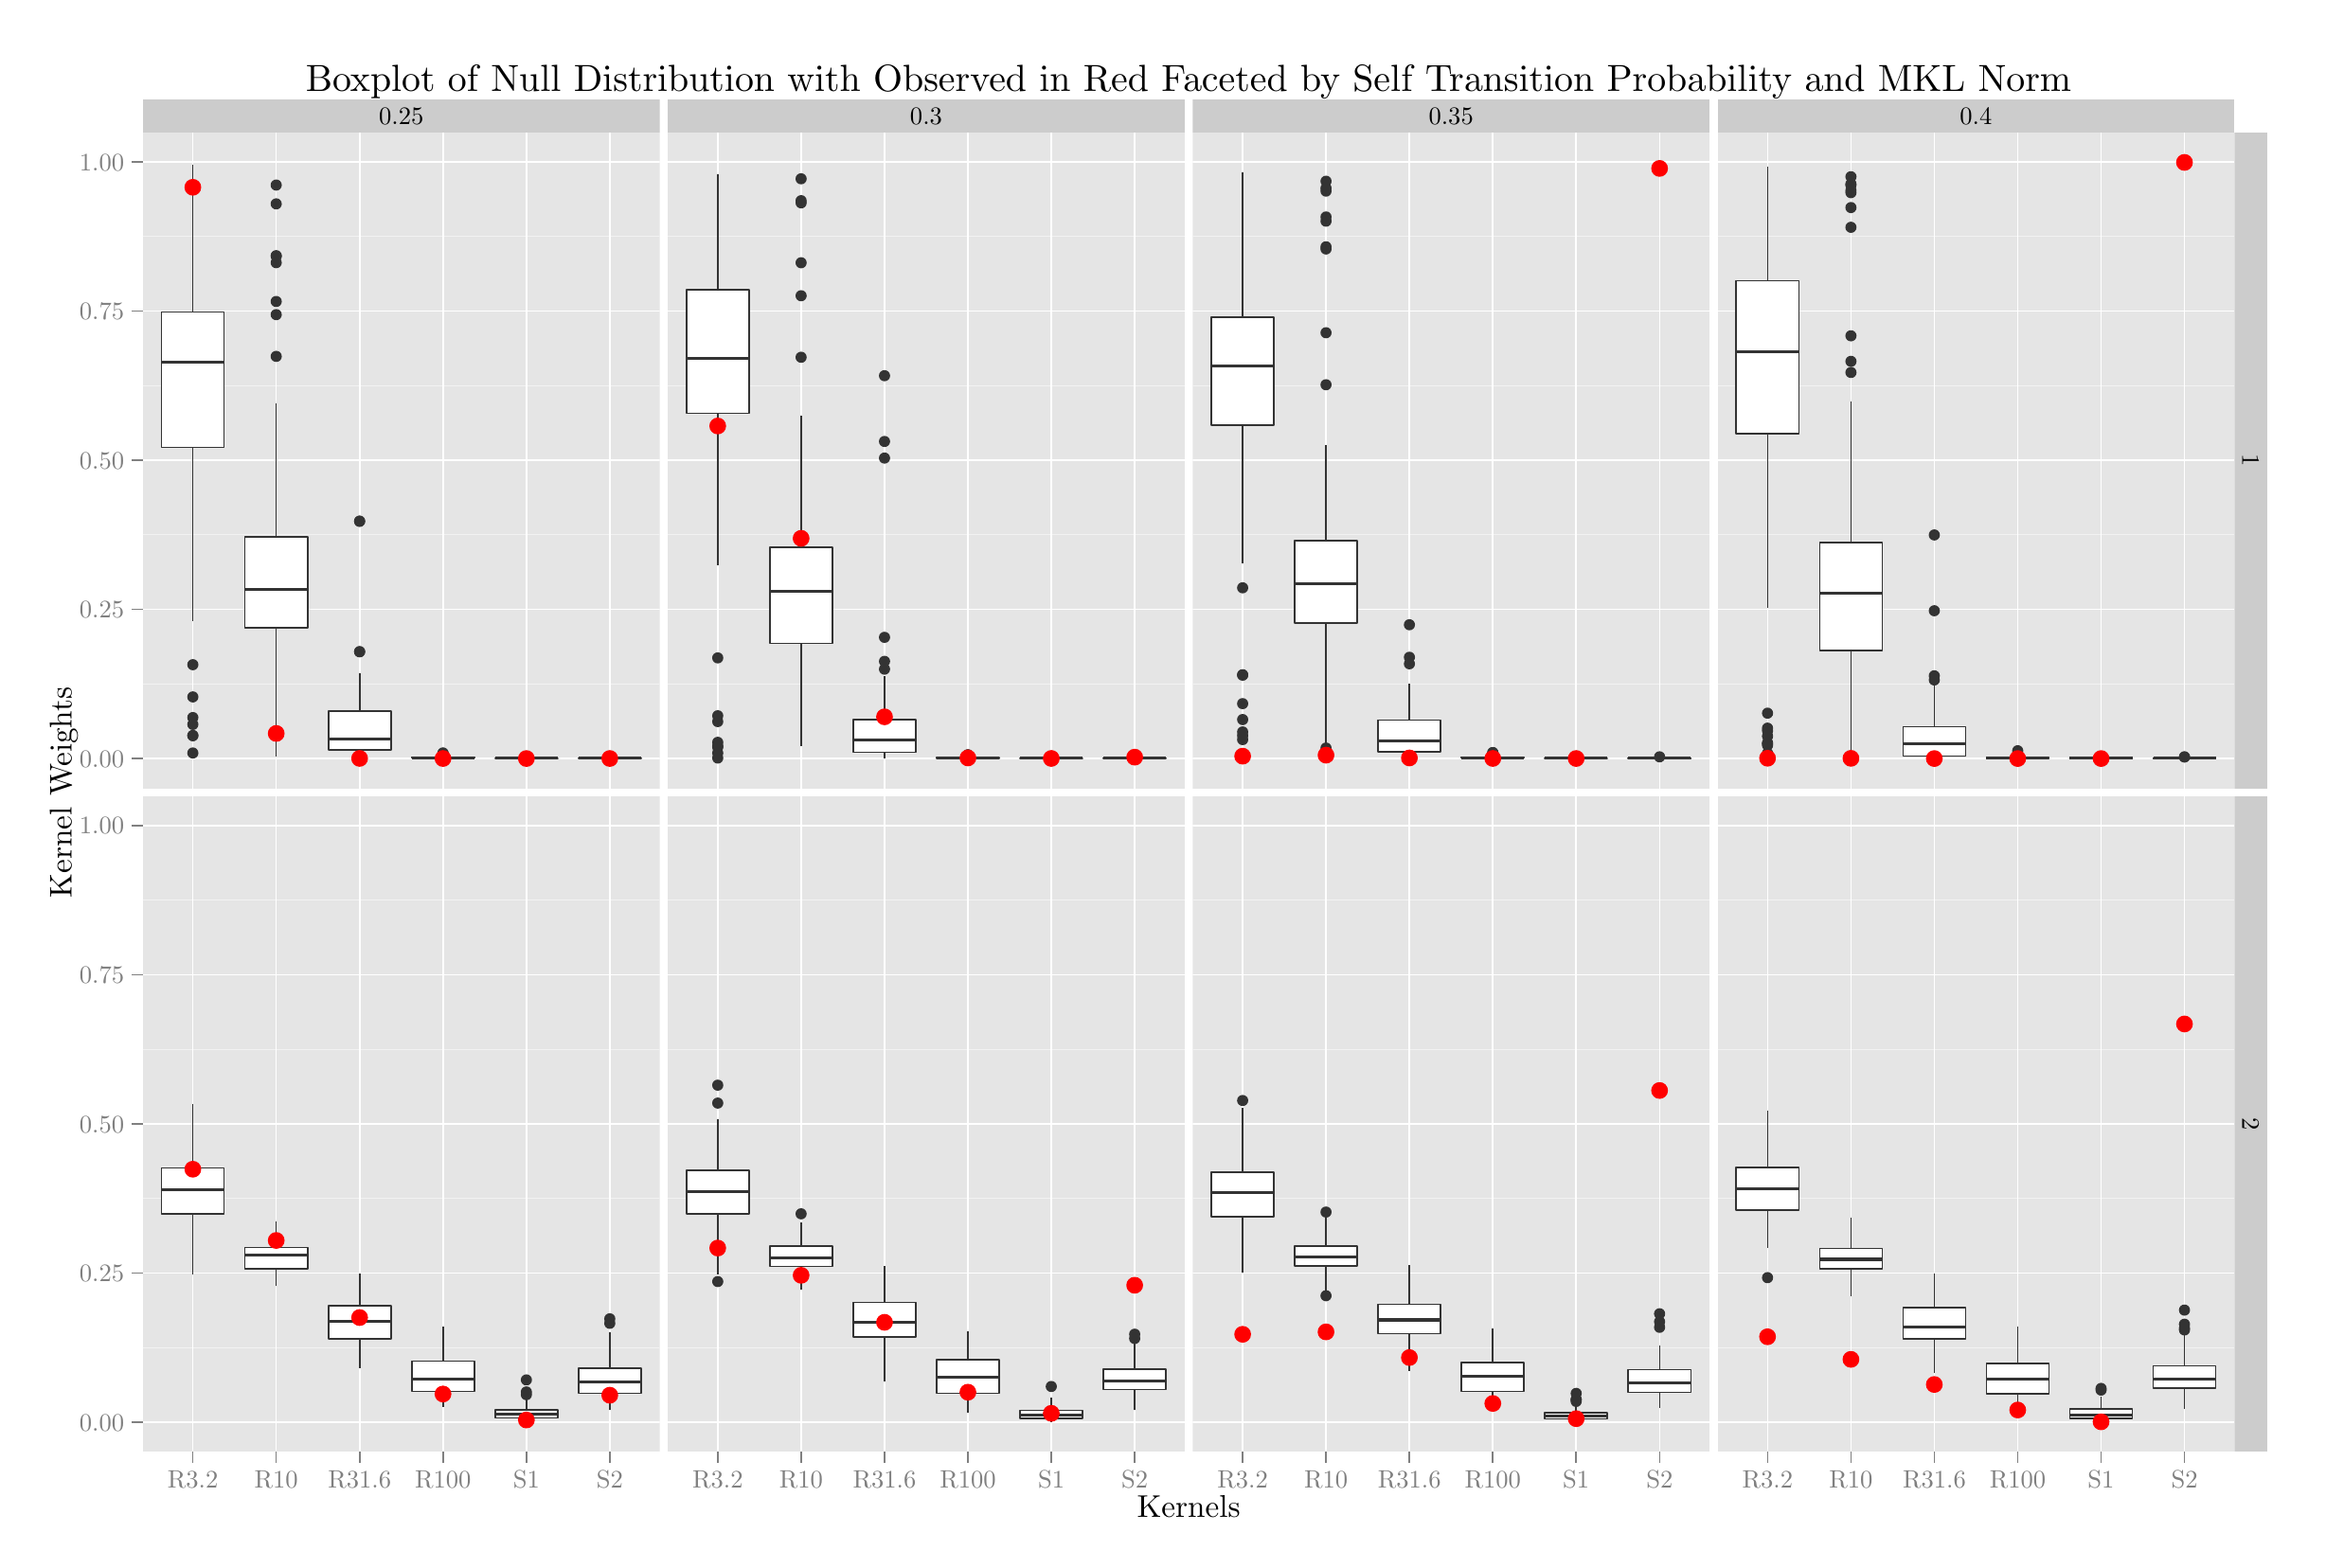
\begin{tikzpicture}[x=1pt,y=1pt]
\definecolor[named]{fillColor}{rgb}{1.00,1.00,1.00}
\path[use as bounding box,fill=fillColor,fill opacity=0.00] (0,0) rectangle (867.24,578.16);
\begin{scope}
\path[clip] (  0.00,  0.00) rectangle (867.24,578.16);
\definecolor[named]{drawColor}{rgb}{1.00,1.00,1.00}
\definecolor[named]{fillColor}{rgb}{1.00,1.00,1.00}

\path[draw=drawColor,line width= 0.6pt,line join=round,line cap=round,fill=fillColor] ( -0.00,  0.00) rectangle (867.24,578.16);
\end{scope}
\begin{scope}
\path[clip] ( 44.49,537.54) rectangle (241.75,550.17);
\definecolor[named]{fillColor}{rgb}{0.80,0.80,0.80}

\path[fill=fillColor] ( 44.49,537.54) rectangle (241.75,550.17);
\definecolor[named]{drawColor}{rgb}{0.00,0.00,0.00}

\node[text=drawColor,anchor=base,inner sep=0pt, outer sep=0pt, scale=  0.96] at (143.12,540.55) {0.25};
\end{scope}
\begin{scope}
\path[clip] (244.76,537.54) rectangle (442.02,550.17);
\definecolor[named]{fillColor}{rgb}{0.80,0.80,0.80}

\path[fill=fillColor] (244.76,537.54) rectangle (442.02,550.17);
\definecolor[named]{drawColor}{rgb}{0.00,0.00,0.00}

\node[text=drawColor,anchor=base,inner sep=0pt, outer sep=0pt, scale=  0.96] at (343.39,540.55) {0.3};
\end{scope}
\begin{scope}
\path[clip] (445.03,537.54) rectangle (642.29,550.17);
\definecolor[named]{fillColor}{rgb}{0.80,0.80,0.80}

\path[fill=fillColor] (445.03,537.54) rectangle (642.29,550.17);
\definecolor[named]{drawColor}{rgb}{0.00,0.00,0.00}

\node[text=drawColor,anchor=base,inner sep=0pt, outer sep=0pt, scale=  0.96] at (543.66,540.55) {0.35};
\end{scope}
\begin{scope}
\path[clip] (645.30,537.54) rectangle (842.56,550.17);
\definecolor[named]{fillColor}{rgb}{0.80,0.80,0.80}

\path[fill=fillColor] (645.30,537.54) rectangle (842.56,550.17);
\definecolor[named]{drawColor}{rgb}{0.00,0.00,0.00}

\node[text=drawColor,anchor=base,inner sep=0pt, outer sep=0pt, scale=  0.96] at (743.93,540.55) {0.4};
\end{scope}
\begin{scope}
\path[clip] ( 44.49,287.29) rectangle (241.75,537.54);
\definecolor[named]{fillColor}{rgb}{0.90,0.90,0.90}

\path[fill=fillColor] ( 44.49,287.29) rectangle (241.75,537.54);
\definecolor[named]{drawColor}{rgb}{0.95,0.95,0.95}

\path[draw=drawColor,line width= 0.3pt,line join=round] ( 44.49,327.13) --
	(241.75,327.13);

\path[draw=drawColor,line width= 0.3pt,line join=round] ( 44.49,384.06) --
	(241.75,384.06);

\path[draw=drawColor,line width= 0.3pt,line join=round] ( 44.49,440.99) --
	(241.75,440.99);

\path[draw=drawColor,line width= 0.3pt,line join=round] ( 44.49,497.92) --
	(241.75,497.92);
\definecolor[named]{drawColor}{rgb}{1.00,1.00,1.00}

\path[draw=drawColor,line width= 0.6pt,line join=round] ( 44.49,298.67) --
	(241.75,298.67);

\path[draw=drawColor,line width= 0.6pt,line join=round] ( 44.49,355.60) --
	(241.75,355.60);

\path[draw=drawColor,line width= 0.6pt,line join=round] ( 44.49,412.52) --
	(241.75,412.52);

\path[draw=drawColor,line width= 0.6pt,line join=round] ( 44.49,469.45) --
	(241.75,469.45);

\path[draw=drawColor,line width= 0.6pt,line join=round] ( 44.49,526.38) --
	(241.75,526.38);

\path[draw=drawColor,line width= 0.6pt,line join=round] ( 63.58,287.29) --
	( 63.58,537.54);

\path[draw=drawColor,line width= 0.6pt,line join=round] ( 95.39,287.29) --
	( 95.39,537.54);

\path[draw=drawColor,line width= 0.6pt,line join=round] (127.21,287.29) --
	(127.21,537.54);

\path[draw=drawColor,line width= 0.6pt,line join=round] (159.02,287.29) --
	(159.02,537.54);

\path[draw=drawColor,line width= 0.6pt,line join=round] (190.84,287.29) --
	(190.84,537.54);

\path[draw=drawColor,line width= 0.6pt,line join=round] (222.66,287.29) --
	(222.66,537.54);
\definecolor[named]{fillColor}{rgb}{0.20,0.20,0.20}

\path[fill=fillColor] ( 63.58,307.38) circle (  2.13);

\path[fill=fillColor] ( 63.58,314.31) circle (  2.13);

\path[fill=fillColor] ( 63.58,307.48) circle (  2.13);

\path[fill=fillColor] ( 63.58,300.79) circle (  2.13);

\path[fill=fillColor] ( 63.58,334.49) circle (  2.13);

\path[fill=fillColor] ( 63.58,311.70) circle (  2.13);

\path[fill=fillColor] ( 63.58,322.19) circle (  2.13);
\definecolor[named]{drawColor}{rgb}{0.20,0.20,0.20}

\path[draw=drawColor,line width= 0.6pt,line join=round,fill=fillColor] ( 63.58,469.10) -- ( 63.58,525.42);

\path[draw=drawColor,line width= 0.6pt,line join=round,fill=fillColor] ( 63.58,417.47) -- ( 63.58,351.27);
\definecolor[named]{fillColor}{rgb}{1.00,1.00,1.00}

\path[draw=drawColor,line width= 0.6pt,line join=round,line cap=round,fill=fillColor] ( 51.64,469.10) --
	( 51.64,417.47) --
	( 75.51,417.47) --
	( 75.51,469.10) --
	( 51.64,469.10) --
	cycle;
\definecolor[named]{fillColor}{rgb}{0.20,0.20,0.20}

\path[draw=drawColor,line width= 1.1pt,line join=round,fill=fillColor] ( 51.64,449.89) -- ( 75.51,449.89);

\path[fill=fillColor] ( 95.39,517.53) circle (  2.13);

\path[fill=fillColor] ( 95.39,510.35) circle (  2.13);

\path[fill=fillColor] ( 95.39,490.57) circle (  2.13);

\path[fill=fillColor] ( 95.39,473.10) circle (  2.13);

\path[fill=fillColor] ( 95.39,468.08) circle (  2.13);

\path[fill=fillColor] ( 95.39,490.38) circle (  2.13);

\path[fill=fillColor] ( 95.39,452.15) circle (  2.13);

\path[fill=fillColor] ( 95.39,487.91) circle (  2.13);

\path[draw=drawColor,line width= 0.6pt,line join=round,fill=fillColor] ( 95.39,383.34) -- ( 95.39,434.24);

\path[draw=drawColor,line width= 0.6pt,line join=round,fill=fillColor] ( 95.39,348.56) -- ( 95.39,299.60);
\definecolor[named]{fillColor}{rgb}{1.00,1.00,1.00}

\path[draw=drawColor,line width= 0.6pt,line join=round,line cap=round,fill=fillColor] ( 83.46,383.34) --
	( 83.46,348.56) --
	(107.32,348.56) --
	(107.32,383.34) --
	( 83.46,383.34) --
	cycle;
\definecolor[named]{fillColor}{rgb}{0.20,0.20,0.20}

\path[draw=drawColor,line width= 1.1pt,line join=round,fill=fillColor] ( 83.46,363.31) -- (107.32,363.31);

\path[fill=fillColor] (127.21,389.19) circle (  2.13);

\path[fill=fillColor] (127.21,339.46) circle (  2.13);

\path[fill=fillColor] (127.21,389.29) circle (  2.13);

\path[fill=fillColor] (127.21,339.43) circle (  2.13);

\path[draw=drawColor,line width= 0.6pt,line join=round,fill=fillColor] (127.21,316.88) -- (127.21,331.41);

\path[draw=drawColor,line width= 0.6pt,line join=round,fill=fillColor] (127.21,301.99) -- (127.21,298.68);
\definecolor[named]{fillColor}{rgb}{1.00,1.00,1.00}

\path[draw=drawColor,line width= 0.6pt,line join=round,line cap=round,fill=fillColor] (115.28,316.88) --
	(115.28,301.99) --
	(139.14,301.99) --
	(139.14,316.88) --
	(115.28,316.88) --
	cycle;
\definecolor[named]{fillColor}{rgb}{0.20,0.20,0.20}

\path[draw=drawColor,line width= 1.1pt,line join=round,fill=fillColor] (115.28,306.04) -- (139.14,306.04);

\path[fill=fillColor] (159.02,300.36) circle (  2.13);

\path[fill=fillColor] (159.02,300.29) circle (  2.13);

\path[fill=fillColor] (159.02,299.94) circle (  2.13);

\path[fill=fillColor] (159.02,300.17) circle (  2.13);

\path[fill=fillColor] (159.02,300.68) circle (  2.13);

\path[fill=fillColor] (159.02,300.80) circle (  2.13);

\path[fill=fillColor] (159.02,300.49) circle (  2.13);

\path[fill=fillColor] (159.02,299.97) circle (  2.13);

\path[fill=fillColor] (159.02,300.05) circle (  2.13);

\path[draw=drawColor,line width= 0.6pt,line join=round,fill=fillColor] (159.02,299.29) -- (159.02,299.82);

\path[draw=drawColor,line width= 0.6pt,line join=round,fill=fillColor] (159.02,298.86) -- (159.02,298.67);
\definecolor[named]{fillColor}{rgb}{1.00,1.00,1.00}

\path[draw=drawColor,line width= 0.6pt,line join=round,line cap=round,fill=fillColor] (147.09,299.29) --
	(147.09,298.86) --
	(170.95,298.86) --
	(170.95,299.29) --
	(147.09,299.29) --
	cycle;
\definecolor[named]{fillColor}{rgb}{0.20,0.20,0.20}

\path[draw=drawColor,line width= 1.1pt,line join=round,fill=fillColor] (147.09,298.99) -- (170.95,298.99);

\path[draw=drawColor,line width= 0.6pt,line join=round,fill=fillColor] (190.84,298.83) -- (190.84,298.97);

\path[draw=drawColor,line width= 0.6pt,line join=round,fill=fillColor] (190.84,298.71) -- (190.84,298.67);
\definecolor[named]{fillColor}{rgb}{1.00,1.00,1.00}

\path[draw=drawColor,line width= 0.6pt,line join=round,line cap=round,fill=fillColor] (178.91,298.83) --
	(178.91,298.71) --
	(202.77,298.71) --
	(202.77,298.83) --
	(178.91,298.83) --
	cycle;
\definecolor[named]{fillColor}{rgb}{0.20,0.20,0.20}

\path[draw=drawColor,line width= 1.1pt,line join=round,fill=fillColor] (178.91,298.78) -- (202.77,298.78);

\path[fill=fillColor] (222.66,299.26) circle (  2.13);

\path[draw=drawColor,line width= 0.6pt,line join=round,fill=fillColor] (222.66,298.94) -- (222.66,299.16);

\path[draw=drawColor,line width= 0.6pt,line join=round,fill=fillColor] (222.66,298.73) -- (222.66,298.67);
\definecolor[named]{fillColor}{rgb}{1.00,1.00,1.00}

\path[draw=drawColor,line width= 0.6pt,line join=round,line cap=round,fill=fillColor] (210.73,298.94) --
	(210.73,298.73) --
	(234.59,298.73) --
	(234.59,298.94) --
	(210.73,298.94) --
	cycle;
\definecolor[named]{fillColor}{rgb}{0.20,0.20,0.20}

\path[draw=drawColor,line width= 1.1pt,line join=round,fill=fillColor] (210.73,298.86) -- (234.59,298.86);
\definecolor[named]{fillColor}{rgb}{1.00,0.00,0.00}

\path[fill=fillColor] ( 63.58,516.68) circle (  3.20);

\path[fill=fillColor] ( 95.39,308.25) circle (  3.20);

\path[fill=fillColor] (127.21,298.73) circle (  3.20);

\path[fill=fillColor] (159.02,298.69) circle (  3.20);

\path[fill=fillColor] (190.84,298.68) circle (  3.20);

\path[fill=fillColor] (222.66,298.69) circle (  3.20);
\end{scope}
\begin{scope}
\path[clip] ( 44.49, 34.03) rectangle (241.75,284.28);
\definecolor[named]{fillColor}{rgb}{0.90,0.90,0.90}

\path[fill=fillColor] ( 44.49, 34.03) rectangle (241.75,284.28);
\definecolor[named]{drawColor}{rgb}{0.95,0.95,0.95}

\path[draw=drawColor,line width= 0.3pt,line join=round] ( 44.49, 73.87) --
	(241.75, 73.87);

\path[draw=drawColor,line width= 0.3pt,line join=round] ( 44.49,130.80) --
	(241.75,130.80);

\path[draw=drawColor,line width= 0.3pt,line join=round] ( 44.49,187.73) --
	(241.75,187.73);

\path[draw=drawColor,line width= 0.3pt,line join=round] ( 44.49,244.66) --
	(241.75,244.66);
\definecolor[named]{drawColor}{rgb}{1.00,1.00,1.00}

\path[draw=drawColor,line width= 0.6pt,line join=round] ( 44.49, 45.41) --
	(241.75, 45.41);

\path[draw=drawColor,line width= 0.6pt,line join=round] ( 44.49,102.34) --
	(241.75,102.34);

\path[draw=drawColor,line width= 0.6pt,line join=round] ( 44.49,159.26) --
	(241.75,159.26);

\path[draw=drawColor,line width= 0.6pt,line join=round] ( 44.49,216.19) --
	(241.75,216.19);

\path[draw=drawColor,line width= 0.6pt,line join=round] ( 44.49,273.12) --
	(241.75,273.12);

\path[draw=drawColor,line width= 0.6pt,line join=round] ( 63.58, 34.03) --
	( 63.58,284.28);

\path[draw=drawColor,line width= 0.6pt,line join=round] ( 95.39, 34.03) --
	( 95.39,284.28);

\path[draw=drawColor,line width= 0.6pt,line join=round] (127.21, 34.03) --
	(127.21,284.28);

\path[draw=drawColor,line width= 0.6pt,line join=round] (159.02, 34.03) --
	(159.02,284.28);

\path[draw=drawColor,line width= 0.6pt,line join=round] (190.84, 34.03) --
	(190.84,284.28);

\path[draw=drawColor,line width= 0.6pt,line join=round] (222.66, 34.03) --
	(222.66,284.28);
\definecolor[named]{drawColor}{rgb}{0.20,0.20,0.20}
\definecolor[named]{fillColor}{rgb}{0.20,0.20,0.20}

\path[draw=drawColor,line width= 0.6pt,line join=round,fill=fillColor] ( 63.58,142.43) -- ( 63.58,166.88);

\path[draw=drawColor,line width= 0.6pt,line join=round,fill=fillColor] ( 63.58,124.91) -- ( 63.58,101.89);
\definecolor[named]{fillColor}{rgb}{1.00,1.00,1.00}

\path[draw=drawColor,line width= 0.6pt,line join=round,line cap=round,fill=fillColor] ( 51.64,142.43) --
	( 51.64,124.91) --
	( 75.51,124.91) --
	( 75.51,142.43) --
	( 51.64,142.43) --
	cycle;
\definecolor[named]{fillColor}{rgb}{0.20,0.20,0.20}

\path[draw=drawColor,line width= 1.1pt,line join=round,fill=fillColor] ( 51.64,134.06) -- ( 75.51,134.06);

\path[draw=drawColor,line width= 0.6pt,line join=round,fill=fillColor] ( 95.39,112.12) -- ( 95.39,122.17);

\path[draw=drawColor,line width= 0.6pt,line join=round,fill=fillColor] ( 95.39,104.05) -- ( 95.39, 97.30);
\definecolor[named]{fillColor}{rgb}{1.00,1.00,1.00}

\path[draw=drawColor,line width= 0.6pt,line join=round,line cap=round,fill=fillColor] ( 83.46,112.12) --
	( 83.46,104.05) --
	(107.32,104.05) --
	(107.32,112.12) --
	( 83.46,112.12) --
	cycle;
\definecolor[named]{fillColor}{rgb}{0.20,0.20,0.20}

\path[draw=drawColor,line width= 1.1pt,line join=round,fill=fillColor] ( 83.46,109.03) -- (107.32,109.03);

\path[draw=drawColor,line width= 0.6pt,line join=round,fill=fillColor] (127.21, 89.76) -- (127.21,101.99);

\path[draw=drawColor,line width= 0.6pt,line join=round,fill=fillColor] (127.21, 77.13) -- (127.21, 66.07);
\definecolor[named]{fillColor}{rgb}{1.00,1.00,1.00}

\path[draw=drawColor,line width= 0.6pt,line join=round,line cap=round,fill=fillColor] (115.28, 89.76) --
	(115.28, 77.13) --
	(139.14, 77.13) --
	(139.14, 89.76) --
	(115.28, 89.76) --
	cycle;
\definecolor[named]{fillColor}{rgb}{0.20,0.20,0.20}

\path[draw=drawColor,line width= 1.1pt,line join=round,fill=fillColor] (115.28, 83.75) -- (139.14, 83.75);

\path[draw=drawColor,line width= 0.6pt,line join=round,fill=fillColor] (159.02, 68.66) -- (159.02, 81.78);

\path[draw=drawColor,line width= 0.6pt,line join=round,fill=fillColor] (159.02, 57.13) -- (159.02, 51.25);
\definecolor[named]{fillColor}{rgb}{1.00,1.00,1.00}

\path[draw=drawColor,line width= 0.6pt,line join=round,line cap=round,fill=fillColor] (147.09, 68.66) --
	(147.09, 57.13) --
	(170.95, 57.13) --
	(170.95, 68.66) --
	(147.09, 68.66) --
	cycle;
\definecolor[named]{fillColor}{rgb}{0.20,0.20,0.20}

\path[draw=drawColor,line width= 1.1pt,line join=round,fill=fillColor] (147.09, 61.99) -- (170.95, 61.99);

\path[fill=fillColor] (190.84, 55.91) circle (  2.13);

\path[fill=fillColor] (190.84, 61.55) circle (  2.13);

\path[fill=fillColor] (190.84, 56.96) circle (  2.13);

\path[draw=drawColor,line width= 0.6pt,line join=round,fill=fillColor] (190.84, 50.14) -- (190.84, 54.71);

\path[draw=drawColor,line width= 0.6pt,line join=round,fill=fillColor] (190.84, 47.08) -- (190.84, 45.57);
\definecolor[named]{fillColor}{rgb}{1.00,1.00,1.00}

\path[draw=drawColor,line width= 0.6pt,line join=round,line cap=round,fill=fillColor] (178.91, 50.14) --
	(178.91, 47.08) --
	(202.77, 47.08) --
	(202.77, 50.14) --
	(178.91, 50.14) --
	cycle;
\definecolor[named]{fillColor}{rgb}{0.20,0.20,0.20}

\path[draw=drawColor,line width= 1.1pt,line join=round,fill=fillColor] (178.91, 48.41) -- (202.77, 48.41);

\path[fill=fillColor] (222.66, 84.85) circle (  2.13);

\path[fill=fillColor] (222.66, 83.13) circle (  2.13);

\path[draw=drawColor,line width= 0.6pt,line join=round,fill=fillColor] (222.66, 65.95) -- (222.66, 79.86);

\path[draw=drawColor,line width= 0.6pt,line join=round,fill=fillColor] (222.66, 56.46) -- (222.66, 49.93);
\definecolor[named]{fillColor}{rgb}{1.00,1.00,1.00}

\path[draw=drawColor,line width= 0.6pt,line join=round,line cap=round,fill=fillColor] (210.73, 65.95) --
	(210.73, 56.46) --
	(234.59, 56.46) --
	(234.59, 65.95) --
	(210.73, 65.95) --
	cycle;
\definecolor[named]{fillColor}{rgb}{0.20,0.20,0.20}

\path[draw=drawColor,line width= 1.1pt,line join=round,fill=fillColor] (210.73, 60.61) -- (234.59, 60.61);
\definecolor[named]{fillColor}{rgb}{1.00,0.00,0.00}

\path[fill=fillColor] ( 63.58,141.95) circle (  3.20);

\path[fill=fillColor] ( 95.39,114.76) circle (  3.20);

\path[fill=fillColor] (127.21, 85.34) circle (  3.20);

\path[fill=fillColor] (159.02, 56.16) circle (  3.20);

\path[fill=fillColor] (190.84, 46.25) circle (  3.20);

\path[fill=fillColor] (222.66, 55.70) circle (  3.20);
\end{scope}
\begin{scope}
\path[clip] (244.76,287.29) rectangle (442.02,537.54);
\definecolor[named]{fillColor}{rgb}{0.90,0.90,0.90}

\path[fill=fillColor] (244.76,287.29) rectangle (442.02,537.54);
\definecolor[named]{drawColor}{rgb}{0.95,0.95,0.95}

\path[draw=drawColor,line width= 0.3pt,line join=round] (244.76,327.13) --
	(442.02,327.13);

\path[draw=drawColor,line width= 0.3pt,line join=round] (244.76,384.06) --
	(442.02,384.06);

\path[draw=drawColor,line width= 0.3pt,line join=round] (244.76,440.99) --
	(442.02,440.99);

\path[draw=drawColor,line width= 0.3pt,line join=round] (244.76,497.92) --
	(442.02,497.92);
\definecolor[named]{drawColor}{rgb}{1.00,1.00,1.00}

\path[draw=drawColor,line width= 0.6pt,line join=round] (244.76,298.67) --
	(442.02,298.67);

\path[draw=drawColor,line width= 0.6pt,line join=round] (244.76,355.60) --
	(442.02,355.60);

\path[draw=drawColor,line width= 0.6pt,line join=round] (244.76,412.52) --
	(442.02,412.52);

\path[draw=drawColor,line width= 0.6pt,line join=round] (244.76,469.45) --
	(442.02,469.45);

\path[draw=drawColor,line width= 0.6pt,line join=round] (244.76,526.38) --
	(442.02,526.38);

\path[draw=drawColor,line width= 0.6pt,line join=round] (263.85,287.29) --
	(263.85,537.54);

\path[draw=drawColor,line width= 0.6pt,line join=round] (295.66,287.29) --
	(295.66,537.54);

\path[draw=drawColor,line width= 0.6pt,line join=round] (327.48,287.29) --
	(327.48,537.54);

\path[draw=drawColor,line width= 0.6pt,line join=round] (359.30,287.29) --
	(359.30,537.54);

\path[draw=drawColor,line width= 0.6pt,line join=round] (391.11,287.29) --
	(391.11,537.54);

\path[draw=drawColor,line width= 0.6pt,line join=round] (422.93,287.29) --
	(422.93,537.54);
\definecolor[named]{fillColor}{rgb}{0.20,0.20,0.20}

\path[fill=fillColor] (263.85,312.78) circle (  2.13);

\path[fill=fillColor] (263.85,303.05) circle (  2.13);

\path[fill=fillColor] (263.85,298.86) circle (  2.13);

\path[fill=fillColor] (263.85,315.00) circle (  2.13);

\path[fill=fillColor] (263.85,300.79) circle (  2.13);

\path[fill=fillColor] (263.85,304.86) circle (  2.13);

\path[fill=fillColor] (263.85,337.08) circle (  2.13);

\path[fill=fillColor] (263.85,303.44) circle (  2.13);
\definecolor[named]{drawColor}{rgb}{0.20,0.20,0.20}

\path[draw=drawColor,line width= 0.6pt,line join=round,fill=fillColor] (263.85,477.54) -- (263.85,521.61);

\path[draw=drawColor,line width= 0.6pt,line join=round,fill=fillColor] (263.85,430.46) -- (263.85,372.39);
\definecolor[named]{fillColor}{rgb}{1.00,1.00,1.00}

\path[draw=drawColor,line width= 0.6pt,line join=round,line cap=round,fill=fillColor] (251.92,477.54) --
	(251.92,430.46) --
	(275.78,430.46) --
	(275.78,477.54) --
	(251.92,477.54) --
	cycle;
\definecolor[named]{fillColor}{rgb}{0.20,0.20,0.20}

\path[draw=drawColor,line width= 1.1pt,line join=round,fill=fillColor] (251.92,451.30) -- (275.78,451.30);

\path[fill=fillColor] (295.66,511.56) circle (  2.13);

\path[fill=fillColor] (295.66,451.82) circle (  2.13);

\path[fill=fillColor] (295.66,510.74) circle (  2.13);

\path[fill=fillColor] (295.66,519.92) circle (  2.13);

\path[fill=fillColor] (295.66,487.88) circle (  2.13);

\path[fill=fillColor] (295.66,475.29) circle (  2.13);

\path[draw=drawColor,line width= 0.6pt,line join=round,fill=fillColor] (295.66,379.19) -- (295.66,429.63);

\path[draw=drawColor,line width= 0.6pt,line join=round,fill=fillColor] (295.66,342.57) -- (295.66,303.36);
\definecolor[named]{fillColor}{rgb}{1.00,1.00,1.00}

\path[draw=drawColor,line width= 0.6pt,line join=round,line cap=round,fill=fillColor] (283.73,379.19) --
	(283.73,342.57) --
	(307.59,342.57) --
	(307.59,379.19) --
	(283.73,379.19) --
	cycle;
\definecolor[named]{fillColor}{rgb}{0.20,0.20,0.20}

\path[draw=drawColor,line width= 1.1pt,line join=round,fill=fillColor] (283.73,362.49) -- (307.59,362.49);

\path[fill=fillColor] (327.48,335.76) circle (  2.13);

\path[fill=fillColor] (327.48,444.77) circle (  2.13);

\path[fill=fillColor] (327.48,332.78) circle (  2.13);

\path[fill=fillColor] (327.48,419.68) circle (  2.13);

\path[fill=fillColor] (327.48,413.34) circle (  2.13);

\path[fill=fillColor] (327.48,344.93) circle (  2.13);

\path[draw=drawColor,line width= 0.6pt,line join=round,fill=fillColor] (327.48,313.54) -- (327.48,330.05);

\path[draw=drawColor,line width= 0.6pt,line join=round,fill=fillColor] (327.48,301.08) -- (327.48,298.70);
\definecolor[named]{fillColor}{rgb}{1.00,1.00,1.00}

\path[draw=drawColor,line width= 0.6pt,line join=round,line cap=round,fill=fillColor] (315.55,313.54) --
	(315.55,301.08) --
	(339.41,301.08) --
	(339.41,313.54) --
	(315.55,313.54) --
	cycle;
\definecolor[named]{fillColor}{rgb}{0.20,0.20,0.20}

\path[draw=drawColor,line width= 1.1pt,line join=round,fill=fillColor] (315.55,305.87) -- (339.41,305.87);

\path[fill=fillColor] (359.30,300.05) circle (  2.13);

\path[fill=fillColor] (359.30,300.11) circle (  2.13);

\path[fill=fillColor] (359.30,299.86) circle (  2.13);

\path[fill=fillColor] (359.30,299.72) circle (  2.13);

\path[fill=fillColor] (359.30,299.80) circle (  2.13);

\path[fill=fillColor] (359.30,299.71) circle (  2.13);

\path[draw=drawColor,line width= 0.6pt,line join=round,fill=fillColor] (359.30,299.16) -- (359.30,299.67);

\path[draw=drawColor,line width= 0.6pt,line join=round,fill=fillColor] (359.30,298.81) -- (359.30,298.68);
\definecolor[named]{fillColor}{rgb}{1.00,1.00,1.00}

\path[draw=drawColor,line width= 0.6pt,line join=round,line cap=round,fill=fillColor] (347.36,299.16) --
	(347.36,298.81) --
	(371.23,298.81) --
	(371.23,299.16) --
	(347.36,299.16) --
	cycle;
\definecolor[named]{fillColor}{rgb}{0.20,0.20,0.20}

\path[draw=drawColor,line width= 1.1pt,line join=round,fill=fillColor] (347.36,298.96) -- (371.23,298.96);

\path[fill=fillColor] (391.11,299.17) circle (  2.13);

\path[fill=fillColor] (391.11,299.08) circle (  2.13);

\path[draw=drawColor,line width= 0.6pt,line join=round,fill=fillColor] (391.11,298.82) -- (391.11,298.97);

\path[draw=drawColor,line width= 0.6pt,line join=round,fill=fillColor] (391.11,298.71) -- (391.11,298.67);
\definecolor[named]{fillColor}{rgb}{1.00,1.00,1.00}

\path[draw=drawColor,line width= 0.6pt,line join=round,line cap=round,fill=fillColor] (379.18,298.82) --
	(379.18,298.71) --
	(403.04,298.71) --
	(403.04,298.82) --
	(379.18,298.82) --
	cycle;
\definecolor[named]{fillColor}{rgb}{0.20,0.20,0.20}

\path[draw=drawColor,line width= 1.1pt,line join=round,fill=fillColor] (379.18,298.77) -- (403.04,298.77);

\path[fill=fillColor] (422.93,299.90) circle (  2.13);

\path[fill=fillColor] (422.93,299.36) circle (  2.13);

\path[fill=fillColor] (422.93,299.32) circle (  2.13);

\path[fill=fillColor] (422.93,299.61) circle (  2.13);

\path[draw=drawColor,line width= 0.6pt,line join=round,fill=fillColor] (422.93,298.90) -- (422.93,299.07);

\path[draw=drawColor,line width= 0.6pt,line join=round,fill=fillColor] (422.93,298.74) -- (422.93,298.67);
\definecolor[named]{fillColor}{rgb}{1.00,1.00,1.00}

\path[draw=drawColor,line width= 0.6pt,line join=round,line cap=round,fill=fillColor] (411.00,298.90) --
	(411.00,298.74) --
	(434.86,298.74) --
	(434.86,298.90) --
	(411.00,298.90) --
	cycle;
\definecolor[named]{fillColor}{rgb}{0.20,0.20,0.20}

\path[draw=drawColor,line width= 1.1pt,line join=round,fill=fillColor] (411.00,298.84) -- (434.86,298.84);
\definecolor[named]{fillColor}{rgb}{1.00,0.00,0.00}

\path[fill=fillColor] (263.85,425.59) circle (  3.20);

\path[fill=fillColor] (295.66,382.71) circle (  3.20);

\path[fill=fillColor] (327.48,314.59) circle (  3.20);

\path[fill=fillColor] (359.30,298.91) circle (  3.20);

\path[fill=fillColor] (391.11,298.71) circle (  3.20);

\path[fill=fillColor] (422.93,299.20) circle (  3.20);
\end{scope}
\begin{scope}
\path[clip] (244.76, 34.03) rectangle (442.02,284.28);
\definecolor[named]{fillColor}{rgb}{0.90,0.90,0.90}

\path[fill=fillColor] (244.76, 34.03) rectangle (442.02,284.28);
\definecolor[named]{drawColor}{rgb}{0.95,0.95,0.95}

\path[draw=drawColor,line width= 0.3pt,line join=round] (244.76, 73.87) --
	(442.02, 73.87);

\path[draw=drawColor,line width= 0.3pt,line join=round] (244.76,130.80) --
	(442.02,130.80);

\path[draw=drawColor,line width= 0.3pt,line join=round] (244.76,187.73) --
	(442.02,187.73);

\path[draw=drawColor,line width= 0.3pt,line join=round] (244.76,244.66) --
	(442.02,244.66);
\definecolor[named]{drawColor}{rgb}{1.00,1.00,1.00}

\path[draw=drawColor,line width= 0.6pt,line join=round] (244.76, 45.41) --
	(442.02, 45.41);

\path[draw=drawColor,line width= 0.6pt,line join=round] (244.76,102.34) --
	(442.02,102.34);

\path[draw=drawColor,line width= 0.6pt,line join=round] (244.76,159.26) --
	(442.02,159.26);

\path[draw=drawColor,line width= 0.6pt,line join=round] (244.76,216.19) --
	(442.02,216.19);

\path[draw=drawColor,line width= 0.6pt,line join=round] (244.76,273.12) --
	(442.02,273.12);

\path[draw=drawColor,line width= 0.6pt,line join=round] (263.85, 34.03) --
	(263.85,284.28);

\path[draw=drawColor,line width= 0.6pt,line join=round] (295.66, 34.03) --
	(295.66,284.28);

\path[draw=drawColor,line width= 0.6pt,line join=round] (327.48, 34.03) --
	(327.48,284.28);

\path[draw=drawColor,line width= 0.6pt,line join=round] (359.30, 34.03) --
	(359.30,284.28);

\path[draw=drawColor,line width= 0.6pt,line join=round] (391.11, 34.03) --
	(391.11,284.28);

\path[draw=drawColor,line width= 0.6pt,line join=round] (422.93, 34.03) --
	(422.93,284.28);
\definecolor[named]{fillColor}{rgb}{0.20,0.20,0.20}

\path[fill=fillColor] (263.85,174.02) circle (  2.13);

\path[fill=fillColor] (263.85,167.19) circle (  2.13);

\path[fill=fillColor] (263.85, 99.08) circle (  2.13);
\definecolor[named]{drawColor}{rgb}{0.20,0.20,0.20}

\path[draw=drawColor,line width= 0.6pt,line join=round,fill=fillColor] (263.85,141.42) -- (263.85,161.04);

\path[draw=drawColor,line width= 0.6pt,line join=round,fill=fillColor] (263.85,125.00) -- (263.85,101.89);
\definecolor[named]{fillColor}{rgb}{1.00,1.00,1.00}

\path[draw=drawColor,line width= 0.6pt,line join=round,line cap=round,fill=fillColor] (251.92,141.42) --
	(251.92,125.00) --
	(275.78,125.00) --
	(275.78,141.42) --
	(251.92,141.42) --
	cycle;
\definecolor[named]{fillColor}{rgb}{0.20,0.20,0.20}

\path[draw=drawColor,line width= 1.1pt,line join=round,fill=fillColor] (251.92,133.50) -- (275.78,133.50);

\path[fill=fillColor] (295.66,124.93) circle (  2.13);

\path[draw=drawColor,line width= 0.6pt,line join=round,fill=fillColor] (295.66,112.62) -- (295.66,121.75);

\path[draw=drawColor,line width= 0.6pt,line join=round,fill=fillColor] (295.66,104.82) -- (295.66, 95.83);
\definecolor[named]{fillColor}{rgb}{1.00,1.00,1.00}

\path[draw=drawColor,line width= 0.6pt,line join=round,line cap=round,fill=fillColor] (283.73,112.62) --
	(283.73,104.82) --
	(307.59,104.82) --
	(307.59,112.62) --
	(283.73,112.62) --
	cycle;
\definecolor[named]{fillColor}{rgb}{0.20,0.20,0.20}

\path[draw=drawColor,line width= 1.1pt,line join=round,fill=fillColor] (283.73,108.02) -- (307.59,108.02);

\path[draw=drawColor,line width= 0.6pt,line join=round,fill=fillColor] (327.48, 91.06) -- (327.48,104.98);

\path[draw=drawColor,line width= 0.6pt,line join=round,fill=fillColor] (327.48, 77.82) -- (327.48, 61.03);
\definecolor[named]{fillColor}{rgb}{1.00,1.00,1.00}

\path[draw=drawColor,line width= 0.6pt,line join=round,line cap=round,fill=fillColor] (315.55, 91.06) --
	(315.55, 77.82) --
	(339.41, 77.82) --
	(339.41, 91.06) --
	(315.55, 91.06) --
	cycle;
\definecolor[named]{fillColor}{rgb}{0.20,0.20,0.20}

\path[draw=drawColor,line width= 1.1pt,line join=round,fill=fillColor] (315.55, 83.58) -- (339.41, 83.58);

\path[draw=drawColor,line width= 0.6pt,line join=round,fill=fillColor] (359.30, 69.18) -- (359.30, 80.17);

\path[draw=drawColor,line width= 0.6pt,line join=round,fill=fillColor] (359.30, 56.38) -- (359.30, 48.93);
\definecolor[named]{fillColor}{rgb}{1.00,1.00,1.00}

\path[draw=drawColor,line width= 0.6pt,line join=round,line cap=round,fill=fillColor] (347.36, 69.18) --
	(347.36, 56.38) --
	(371.23, 56.38) --
	(371.23, 69.18) --
	(347.36, 69.18) --
	cycle;
\definecolor[named]{fillColor}{rgb}{0.20,0.20,0.20}

\path[draw=drawColor,line width= 1.1pt,line join=round,fill=fillColor] (347.36, 62.45) -- (371.23, 62.45);

\path[fill=fillColor] (391.11, 59.03) circle (  2.13);

\path[draw=drawColor,line width= 0.6pt,line join=round,fill=fillColor] (391.11, 49.97) -- (391.11, 54.75);

\path[draw=drawColor,line width= 0.6pt,line join=round,fill=fillColor] (391.11, 46.78) -- (391.11, 45.54);
\definecolor[named]{fillColor}{rgb}{1.00,1.00,1.00}

\path[draw=drawColor,line width= 0.6pt,line join=round,line cap=round,fill=fillColor] (379.18, 49.97) --
	(379.18, 46.78) --
	(403.04, 46.78) --
	(403.04, 49.97) --
	(379.18, 49.97) --
	cycle;
\definecolor[named]{fillColor}{rgb}{0.20,0.20,0.20}

\path[draw=drawColor,line width= 1.1pt,line join=round,fill=fillColor] (379.18, 48.23) -- (403.04, 48.23);

\path[fill=fillColor] (422.93, 77.34) circle (  2.13);

\path[fill=fillColor] (422.93, 78.99) circle (  2.13);

\path[draw=drawColor,line width= 0.6pt,line join=round,fill=fillColor] (422.93, 65.57) -- (422.93, 76.98);

\path[draw=drawColor,line width= 0.6pt,line join=round,fill=fillColor] (422.93, 57.90) -- (422.93, 50.19);
\definecolor[named]{fillColor}{rgb}{1.00,1.00,1.00}

\path[draw=drawColor,line width= 0.6pt,line join=round,line cap=round,fill=fillColor] (411.00, 65.57) --
	(411.00, 57.90) --
	(434.86, 57.90) --
	(434.86, 65.57) --
	(411.00, 65.57) --
	cycle;
\definecolor[named]{fillColor}{rgb}{0.20,0.20,0.20}

\path[draw=drawColor,line width= 1.1pt,line join=round,fill=fillColor] (411.00, 61.22) -- (434.86, 61.22);
\definecolor[named]{fillColor}{rgb}{1.00,0.00,0.00}

\path[fill=fillColor] (263.85,111.87) circle (  3.20);

\path[fill=fillColor] (295.66,101.46) circle (  3.20);

\path[fill=fillColor] (327.48, 83.52) circle (  3.20);

\path[fill=fillColor] (359.30, 56.85) circle (  3.20);

\path[fill=fillColor] (391.11, 48.79) circle (  3.20);

\path[fill=fillColor] (422.93, 97.67) circle (  3.20);
\end{scope}
\begin{scope}
\path[clip] (445.03,287.29) rectangle (642.29,537.54);
\definecolor[named]{fillColor}{rgb}{0.90,0.90,0.90}

\path[fill=fillColor] (445.03,287.29) rectangle (642.29,537.54);
\definecolor[named]{drawColor}{rgb}{0.95,0.95,0.95}

\path[draw=drawColor,line width= 0.3pt,line join=round] (445.03,327.13) --
	(642.29,327.13);

\path[draw=drawColor,line width= 0.3pt,line join=round] (445.03,384.06) --
	(642.29,384.06);

\path[draw=drawColor,line width= 0.3pt,line join=round] (445.03,440.99) --
	(642.29,440.99);

\path[draw=drawColor,line width= 0.3pt,line join=round] (445.03,497.92) --
	(642.29,497.92);
\definecolor[named]{drawColor}{rgb}{1.00,1.00,1.00}

\path[draw=drawColor,line width= 0.6pt,line join=round] (445.03,298.67) --
	(642.29,298.67);

\path[draw=drawColor,line width= 0.6pt,line join=round] (445.03,355.60) --
	(642.29,355.60);

\path[draw=drawColor,line width= 0.6pt,line join=round] (445.03,412.52) --
	(642.29,412.52);

\path[draw=drawColor,line width= 0.6pt,line join=round] (445.03,469.45) --
	(642.29,469.45);

\path[draw=drawColor,line width= 0.6pt,line join=round] (445.03,526.38) --
	(642.29,526.38);

\path[draw=drawColor,line width= 0.6pt,line join=round] (464.12,287.29) --
	(464.12,537.54);

\path[draw=drawColor,line width= 0.6pt,line join=round] (495.93,287.29) --
	(495.93,537.54);

\path[draw=drawColor,line width= 0.6pt,line join=round] (527.75,287.29) --
	(527.75,537.54);

\path[draw=drawColor,line width= 0.6pt,line join=round] (559.57,287.29) --
	(559.57,537.54);

\path[draw=drawColor,line width= 0.6pt,line join=round] (591.38,287.29) --
	(591.38,537.54);

\path[draw=drawColor,line width= 0.6pt,line join=round] (623.20,287.29) --
	(623.20,537.54);
\definecolor[named]{fillColor}{rgb}{0.20,0.20,0.20}

\path[fill=fillColor] (464.12,313.55) circle (  2.13);

\path[fill=fillColor] (464.12,305.91) circle (  2.13);

\path[fill=fillColor] (464.12,307.44) circle (  2.13);

\path[fill=fillColor] (464.12,330.66) circle (  2.13);

\path[fill=fillColor] (464.12,363.83) circle (  2.13);

\path[fill=fillColor] (464.12,330.49) circle (  2.13);

\path[fill=fillColor] (464.12,319.63) circle (  2.13);

\path[fill=fillColor] (464.12,308.84) circle (  2.13);
\definecolor[named]{drawColor}{rgb}{0.20,0.20,0.20}

\path[draw=drawColor,line width= 0.6pt,line join=round,fill=fillColor] (464.12,467.04) -- (464.12,522.31);

\path[draw=drawColor,line width= 0.6pt,line join=round,fill=fillColor] (464.12,425.93) -- (464.12,373.24);
\definecolor[named]{fillColor}{rgb}{1.00,1.00,1.00}

\path[draw=drawColor,line width= 0.6pt,line join=round,line cap=round,fill=fillColor] (452.19,467.04) --
	(452.19,425.93) --
	(476.05,425.93) --
	(476.05,467.04) --
	(452.19,467.04) --
	cycle;
\definecolor[named]{fillColor}{rgb}{0.20,0.20,0.20}

\path[draw=drawColor,line width= 1.1pt,line join=round,fill=fillColor] (452.19,448.59) -- (476.05,448.59);

\path[fill=fillColor] (495.93,503.74) circle (  2.13);

\path[fill=fillColor] (495.93,519.00) circle (  2.13);

\path[fill=fillColor] (495.93,516.34) circle (  2.13);

\path[fill=fillColor] (495.93,302.68) circle (  2.13);

\path[fill=fillColor] (495.93,493.14) circle (  2.13);

\path[fill=fillColor] (495.93,461.18) circle (  2.13);

\path[fill=fillColor] (495.93,441.32) circle (  2.13);

\path[fill=fillColor] (495.93,493.96) circle (  2.13);

\path[fill=fillColor] (495.93,505.36) circle (  2.13);

\path[fill=fillColor] (495.93,515.22) circle (  2.13);

\path[draw=drawColor,line width= 0.6pt,line join=round,fill=fillColor] (495.93,381.71) -- (495.93,418.31);

\path[draw=drawColor,line width= 0.6pt,line join=round,fill=fillColor] (495.93,350.49) -- (495.93,303.69);
\definecolor[named]{fillColor}{rgb}{1.00,1.00,1.00}

\path[draw=drawColor,line width= 0.6pt,line join=round,line cap=round,fill=fillColor] (484.00,381.71) --
	(484.00,350.49) --
	(507.87,350.49) --
	(507.87,381.71) --
	(484.00,381.71) --
	cycle;
\definecolor[named]{fillColor}{rgb}{0.20,0.20,0.20}

\path[draw=drawColor,line width= 1.1pt,line join=round,fill=fillColor] (484.00,365.46) -- (507.87,365.46);

\path[fill=fillColor] (527.75,349.73) circle (  2.13);

\path[fill=fillColor] (527.75,334.83) circle (  2.13);

\path[fill=fillColor] (527.75,337.33) circle (  2.13);

\path[draw=drawColor,line width= 0.6pt,line join=round,fill=fillColor] (527.75,313.40) -- (527.75,327.13);

\path[draw=drawColor,line width= 0.6pt,line join=round,fill=fillColor] (527.75,301.22) -- (527.75,298.69);
\definecolor[named]{fillColor}{rgb}{1.00,1.00,1.00}

\path[draw=drawColor,line width= 0.6pt,line join=round,line cap=round,fill=fillColor] (515.82,313.40) --
	(515.82,301.22) --
	(539.68,301.22) --
	(539.68,313.40) --
	(515.82,313.40) --
	cycle;
\definecolor[named]{fillColor}{rgb}{0.20,0.20,0.20}

\path[draw=drawColor,line width= 1.1pt,line join=round,fill=fillColor] (515.82,305.49) -- (539.68,305.49);

\path[fill=fillColor] (559.57,299.99) circle (  2.13);

\path[fill=fillColor] (559.57,300.96) circle (  2.13);

\path[fill=fillColor] (559.57,300.90) circle (  2.13);

\path[fill=fillColor] (559.57,299.85) circle (  2.13);

\path[fill=fillColor] (559.57,300.60) circle (  2.13);

\path[draw=drawColor,line width= 0.6pt,line join=round,fill=fillColor] (559.57,299.22) -- (559.57,299.79);

\path[draw=drawColor,line width= 0.6pt,line join=round,fill=fillColor] (559.57,298.84) -- (559.57,298.67);
\definecolor[named]{fillColor}{rgb}{1.00,1.00,1.00}

\path[draw=drawColor,line width= 0.6pt,line join=round,line cap=round,fill=fillColor] (547.64,299.22) --
	(547.64,298.84) --
	(571.50,298.84) --
	(571.50,299.22) --
	(547.64,299.22) --
	cycle;
\definecolor[named]{fillColor}{rgb}{0.20,0.20,0.20}

\path[draw=drawColor,line width= 1.1pt,line join=round,fill=fillColor] (547.64,298.99) -- (571.50,298.99);

\path[fill=fillColor] (591.38,299.08) circle (  2.13);

\path[draw=drawColor,line width= 0.6pt,line join=round,fill=fillColor] (591.38,298.82) -- (591.38,298.97);

\path[draw=drawColor,line width= 0.6pt,line join=round,fill=fillColor] (591.38,298.71) -- (591.38,298.67);
\definecolor[named]{fillColor}{rgb}{1.00,1.00,1.00}

\path[draw=drawColor,line width= 0.6pt,line join=round,line cap=round,fill=fillColor] (579.45,298.82) --
	(579.45,298.71) --
	(603.31,298.71) --
	(603.31,298.82) --
	(579.45,298.82) --
	cycle;
\definecolor[named]{fillColor}{rgb}{0.20,0.20,0.20}

\path[draw=drawColor,line width= 1.1pt,line join=round,fill=fillColor] (579.45,298.78) -- (603.31,298.78);

\path[fill=fillColor] (623.20,299.33) circle (  2.13);

\path[draw=drawColor,line width= 0.6pt,line join=round,fill=fillColor] (623.20,298.92) -- (623.20,299.11);

\path[draw=drawColor,line width= 0.6pt,line join=round,fill=fillColor] (623.20,298.74) -- (623.20,298.67);
\definecolor[named]{fillColor}{rgb}{1.00,1.00,1.00}

\path[draw=drawColor,line width= 0.6pt,line join=round,line cap=round,fill=fillColor] (611.27,298.92) --
	(611.27,298.74) --
	(635.13,298.74) --
	(635.13,298.92) --
	(611.27,298.92) --
	cycle;
\definecolor[named]{fillColor}{rgb}{0.20,0.20,0.20}

\path[draw=drawColor,line width= 1.1pt,line join=round,fill=fillColor] (611.27,298.83) -- (635.13,298.83);
\definecolor[named]{fillColor}{rgb}{1.00,0.00,0.00}

\path[fill=fillColor] (464.12,299.58) circle (  3.20);

\path[fill=fillColor] (495.93,299.97) circle (  3.20);

\path[fill=fillColor] (527.75,298.90) circle (  3.20);

\path[fill=fillColor] (559.57,298.70) circle (  3.20);

\path[fill=fillColor] (591.38,298.69) circle (  3.20);

\path[fill=fillColor] (623.20,523.88) circle (  3.20);
\end{scope}
\begin{scope}
\path[clip] (445.03, 34.03) rectangle (642.29,284.28);
\definecolor[named]{fillColor}{rgb}{0.90,0.90,0.90}

\path[fill=fillColor] (445.03, 34.03) rectangle (642.29,284.28);
\definecolor[named]{drawColor}{rgb}{0.95,0.95,0.95}

\path[draw=drawColor,line width= 0.3pt,line join=round] (445.03, 73.87) --
	(642.29, 73.87);

\path[draw=drawColor,line width= 0.3pt,line join=round] (445.03,130.80) --
	(642.29,130.80);

\path[draw=drawColor,line width= 0.3pt,line join=round] (445.03,187.73) --
	(642.29,187.73);

\path[draw=drawColor,line width= 0.3pt,line join=round] (445.03,244.66) --
	(642.29,244.66);
\definecolor[named]{drawColor}{rgb}{1.00,1.00,1.00}

\path[draw=drawColor,line width= 0.6pt,line join=round] (445.03, 45.41) --
	(642.29, 45.41);

\path[draw=drawColor,line width= 0.6pt,line join=round] (445.03,102.34) --
	(642.29,102.34);

\path[draw=drawColor,line width= 0.6pt,line join=round] (445.03,159.26) --
	(642.29,159.26);

\path[draw=drawColor,line width= 0.6pt,line join=round] (445.03,216.19) --
	(642.29,216.19);

\path[draw=drawColor,line width= 0.6pt,line join=round] (445.03,273.12) --
	(642.29,273.12);

\path[draw=drawColor,line width= 0.6pt,line join=round] (464.12, 34.03) --
	(464.12,284.28);

\path[draw=drawColor,line width= 0.6pt,line join=round] (495.93, 34.03) --
	(495.93,284.28);

\path[draw=drawColor,line width= 0.6pt,line join=round] (527.75, 34.03) --
	(527.75,284.28);

\path[draw=drawColor,line width= 0.6pt,line join=round] (559.57, 34.03) --
	(559.57,284.28);

\path[draw=drawColor,line width= 0.6pt,line join=round] (591.38, 34.03) --
	(591.38,284.28);

\path[draw=drawColor,line width= 0.6pt,line join=round] (623.20, 34.03) --
	(623.20,284.28);
\definecolor[named]{fillColor}{rgb}{0.20,0.20,0.20}

\path[fill=fillColor] (464.12,168.17) circle (  2.13);
\definecolor[named]{drawColor}{rgb}{0.20,0.20,0.20}

\path[draw=drawColor,line width= 0.6pt,line join=round,fill=fillColor] (464.12,140.78) -- (464.12,165.29);

\path[draw=drawColor,line width= 0.6pt,line join=round,fill=fillColor] (464.12,123.79) -- (464.12,102.65);
\definecolor[named]{fillColor}{rgb}{1.00,1.00,1.00}

\path[draw=drawColor,line width= 0.6pt,line join=round,line cap=round,fill=fillColor] (452.19,140.78) --
	(452.19,123.79) --
	(476.05,123.79) --
	(476.05,140.78) --
	(452.19,140.78) --
	cycle;
\definecolor[named]{fillColor}{rgb}{0.20,0.20,0.20}

\path[draw=drawColor,line width= 1.1pt,line join=round,fill=fillColor] (452.19,133.03) -- (476.05,133.03);

\path[fill=fillColor] (495.93, 93.67) circle (  2.13);

\path[fill=fillColor] (495.93,125.60) circle (  2.13);

\path[draw=drawColor,line width= 0.6pt,line join=round,fill=fillColor] (495.93,112.53) -- (495.93,123.43);

\path[draw=drawColor,line width= 0.6pt,line join=round,fill=fillColor] (495.93,104.99) -- (495.93, 95.54);
\definecolor[named]{fillColor}{rgb}{1.00,1.00,1.00}

\path[draw=drawColor,line width= 0.6pt,line join=round,line cap=round,fill=fillColor] (484.00,112.53) --
	(484.00,104.99) --
	(507.87,104.99) --
	(507.87,112.53) --
	(484.00,112.53) --
	cycle;
\definecolor[named]{fillColor}{rgb}{0.20,0.20,0.20}

\path[draw=drawColor,line width= 1.1pt,line join=round,fill=fillColor] (484.00,108.50) -- (507.87,108.50);

\path[draw=drawColor,line width= 0.6pt,line join=round,fill=fillColor] (527.75, 90.35) -- (527.75,105.30);

\path[draw=drawColor,line width= 0.6pt,line join=round,fill=fillColor] (527.75, 79.20) -- (527.75, 64.87);
\definecolor[named]{fillColor}{rgb}{1.00,1.00,1.00}

\path[draw=drawColor,line width= 0.6pt,line join=round,line cap=round,fill=fillColor] (515.82, 90.35) --
	(515.82, 79.20) --
	(539.68, 79.20) --
	(539.68, 90.35) --
	(515.82, 90.35) --
	cycle;
\definecolor[named]{fillColor}{rgb}{0.20,0.20,0.20}

\path[draw=drawColor,line width= 1.1pt,line join=round,fill=fillColor] (515.82, 84.43) -- (539.68, 84.43);

\path[draw=drawColor,line width= 0.6pt,line join=round,fill=fillColor] (559.57, 68.17) -- (559.57, 81.02);

\path[draw=drawColor,line width= 0.6pt,line join=round,fill=fillColor] (559.57, 57.17) -- (559.57, 50.66);
\definecolor[named]{fillColor}{rgb}{1.00,1.00,1.00}

\path[draw=drawColor,line width= 0.6pt,line join=round,line cap=round,fill=fillColor] (547.64, 68.17) --
	(547.64, 57.17) --
	(571.50, 57.17) --
	(571.50, 68.17) --
	(547.64, 68.17) --
	cycle;
\definecolor[named]{fillColor}{rgb}{0.20,0.20,0.20}

\path[draw=drawColor,line width= 1.1pt,line join=round,fill=fillColor] (547.64, 63.10) -- (571.50, 63.10);

\path[fill=fillColor] (591.38, 54.07) circle (  2.13);

\path[fill=fillColor] (591.38, 53.33) circle (  2.13);

\path[fill=fillColor] (591.38, 56.40) circle (  2.13);

\path[fill=fillColor] (591.38, 54.04) circle (  2.13);

\path[draw=drawColor,line width= 0.6pt,line join=round,fill=fillColor] (591.38, 48.95) -- (591.38, 52.31);

\path[draw=drawColor,line width= 0.6pt,line join=round,fill=fillColor] (591.38, 46.64) -- (591.38, 45.45);
\definecolor[named]{fillColor}{rgb}{1.00,1.00,1.00}

\path[draw=drawColor,line width= 0.6pt,line join=round,line cap=round,fill=fillColor] (579.45, 48.95) --
	(579.45, 46.64) --
	(603.31, 46.64) --
	(603.31, 48.95) --
	(579.45, 48.95) --
	cycle;
\definecolor[named]{fillColor}{rgb}{0.20,0.20,0.20}

\path[draw=drawColor,line width= 1.1pt,line join=round,fill=fillColor] (579.45, 47.86) -- (603.31, 47.86);

\path[fill=fillColor] (623.20, 83.75) circle (  2.13);

\path[fill=fillColor] (623.20, 86.79) circle (  2.13);

\path[fill=fillColor] (623.20, 81.62) circle (  2.13);

\path[draw=drawColor,line width= 0.6pt,line join=round,fill=fillColor] (623.20, 65.42) -- (623.20, 74.77);

\path[draw=drawColor,line width= 0.6pt,line join=round,fill=fillColor] (623.20, 56.83) -- (623.20, 50.85);
\definecolor[named]{fillColor}{rgb}{1.00,1.00,1.00}

\path[draw=drawColor,line width= 0.6pt,line join=round,line cap=round,fill=fillColor] (611.27, 65.42) --
	(611.27, 56.83) --
	(635.13, 56.83) --
	(635.13, 65.42) --
	(611.27, 65.42) --
	cycle;
\definecolor[named]{fillColor}{rgb}{0.20,0.20,0.20}

\path[draw=drawColor,line width= 1.1pt,line join=round,fill=fillColor] (611.27, 60.34) -- (635.13, 60.34);
\definecolor[named]{fillColor}{rgb}{1.00,0.00,0.00}

\path[fill=fillColor] (464.12, 78.95) circle (  3.20);

\path[fill=fillColor] (495.93, 79.86) circle (  3.20);

\path[fill=fillColor] (527.75, 70.07) circle (  3.20);

\path[fill=fillColor] (559.57, 52.55) circle (  3.20);

\path[fill=fillColor] (591.38, 46.75) circle (  3.20);

\path[fill=fillColor] (623.20,171.99) circle (  3.20);
\end{scope}
\begin{scope}
\path[clip] (645.30,287.29) rectangle (842.56,537.54);
\definecolor[named]{fillColor}{rgb}{0.90,0.90,0.90}

\path[fill=fillColor] (645.30,287.29) rectangle (842.56,537.54);
\definecolor[named]{drawColor}{rgb}{0.95,0.95,0.95}

\path[draw=drawColor,line width= 0.3pt,line join=round] (645.30,327.13) --
	(842.56,327.13);

\path[draw=drawColor,line width= 0.3pt,line join=round] (645.30,384.06) --
	(842.56,384.06);

\path[draw=drawColor,line width= 0.3pt,line join=round] (645.30,440.99) --
	(842.56,440.99);

\path[draw=drawColor,line width= 0.3pt,line join=round] (645.30,497.92) --
	(842.56,497.92);
\definecolor[named]{drawColor}{rgb}{1.00,1.00,1.00}

\path[draw=drawColor,line width= 0.6pt,line join=round] (645.30,298.67) --
	(842.56,298.67);

\path[draw=drawColor,line width= 0.6pt,line join=round] (645.30,355.60) --
	(842.56,355.60);

\path[draw=drawColor,line width= 0.6pt,line join=round] (645.30,412.52) --
	(842.56,412.52);

\path[draw=drawColor,line width= 0.6pt,line join=round] (645.30,469.45) --
	(842.56,469.45);

\path[draw=drawColor,line width= 0.6pt,line join=round] (645.30,526.38) --
	(842.56,526.38);

\path[draw=drawColor,line width= 0.6pt,line join=round] (664.39,287.29) --
	(664.39,537.54);

\path[draw=drawColor,line width= 0.6pt,line join=round] (696.21,287.29) --
	(696.21,537.54);

\path[draw=drawColor,line width= 0.6pt,line join=round] (728.02,287.29) --
	(728.02,537.54);

\path[draw=drawColor,line width= 0.6pt,line join=round] (759.84,287.29) --
	(759.84,537.54);

\path[draw=drawColor,line width= 0.6pt,line join=round] (791.65,287.29) --
	(791.65,537.54);

\path[draw=drawColor,line width= 0.6pt,line join=round] (823.47,287.29) --
	(823.47,537.54);
\definecolor[named]{fillColor}{rgb}{0.20,0.20,0.20}

\path[fill=fillColor] (664.39,310.27) circle (  2.13);

\path[fill=fillColor] (664.39,307.22) circle (  2.13);

\path[fill=fillColor] (664.39,304.31) circle (  2.13);

\path[fill=fillColor] (664.39,304.67) circle (  2.13);

\path[fill=fillColor] (664.39,303.72) circle (  2.13);

\path[fill=fillColor] (664.39,315.99) circle (  2.13);

\path[fill=fillColor] (664.39,309.29) circle (  2.13);

\path[fill=fillColor] (664.39,300.73) circle (  2.13);
\definecolor[named]{drawColor}{rgb}{0.20,0.20,0.20}

\path[draw=drawColor,line width= 0.6pt,line join=round,fill=fillColor] (664.39,481.06) -- (664.39,524.39);

\path[draw=drawColor,line width= 0.6pt,line join=round,fill=fillColor] (664.39,422.59) -- (664.39,356.27);
\definecolor[named]{fillColor}{rgb}{1.00,1.00,1.00}

\path[draw=drawColor,line width= 0.6pt,line join=round,line cap=round,fill=fillColor] (652.46,481.06) --
	(652.46,422.59) --
	(676.32,422.59) --
	(676.32,481.06) --
	(652.46,481.06) --
	cycle;
\definecolor[named]{fillColor}{rgb}{0.20,0.20,0.20}

\path[draw=drawColor,line width= 1.1pt,line join=round,fill=fillColor] (652.46,453.80) -- (676.32,453.80);

\path[fill=fillColor] (696.21,450.25) circle (  2.13);

\path[fill=fillColor] (696.21,460.00) circle (  2.13);

\path[fill=fillColor] (696.21,514.62) circle (  2.13);

\path[fill=fillColor] (696.21,517.51) circle (  2.13);

\path[fill=fillColor] (696.21,517.96) circle (  2.13);

\path[fill=fillColor] (696.21,520.71) circle (  2.13);

\path[fill=fillColor] (696.21,508.94) circle (  2.13);

\path[fill=fillColor] (696.21,515.50) circle (  2.13);

\path[fill=fillColor] (696.21,501.41) circle (  2.13);

\path[fill=fillColor] (696.21,446.01) circle (  2.13);

\path[draw=drawColor,line width= 0.6pt,line join=round,fill=fillColor] (696.21,381.20) -- (696.21,435.02);

\path[draw=drawColor,line width= 0.6pt,line join=round,fill=fillColor] (696.21,339.91) -- (696.21,300.59);
\definecolor[named]{fillColor}{rgb}{1.00,1.00,1.00}

\path[draw=drawColor,line width= 0.6pt,line join=round,line cap=round,fill=fillColor] (684.28,381.20) --
	(684.28,339.91) --
	(708.14,339.91) --
	(708.14,381.20) --
	(684.28,381.20) --
	cycle;
\definecolor[named]{fillColor}{rgb}{0.20,0.20,0.20}

\path[draw=drawColor,line width= 1.1pt,line join=round,fill=fillColor] (684.28,361.68) -- (708.14,361.68);

\path[fill=fillColor] (728.02,355.08) circle (  2.13);

\path[fill=fillColor] (728.02,384.00) circle (  2.13);

\path[fill=fillColor] (728.02,330.24) circle (  2.13);

\path[fill=fillColor] (728.02,328.67) circle (  2.13);

\path[draw=drawColor,line width= 0.6pt,line join=round,fill=fillColor] (728.02,310.80) -- (728.02,326.94);

\path[draw=drawColor,line width= 0.6pt,line join=round,fill=fillColor] (728.02,299.65) -- (728.02,298.69);
\definecolor[named]{fillColor}{rgb}{1.00,1.00,1.00}

\path[draw=drawColor,line width= 0.6pt,line join=round,line cap=round,fill=fillColor] (716.09,310.80) --
	(716.09,299.65) --
	(739.95,299.65) --
	(739.95,310.80) --
	(716.09,310.80) --
	cycle;
\definecolor[named]{fillColor}{rgb}{0.20,0.20,0.20}

\path[draw=drawColor,line width= 1.1pt,line join=round,fill=fillColor] (716.09,304.29) -- (739.95,304.29);

\path[fill=fillColor] (759.84,299.78) circle (  2.13);

\path[fill=fillColor] (759.84,301.65) circle (  2.13);

\path[fill=fillColor] (759.84,300.28) circle (  2.13);

\path[fill=fillColor] (759.84,299.85) circle (  2.13);

\path[draw=drawColor,line width= 0.6pt,line join=round,fill=fillColor] (759.84,299.16) -- (759.84,299.72);

\path[draw=drawColor,line width= 0.6pt,line join=round,fill=fillColor] (759.84,298.76) -- (759.84,298.68);
\definecolor[named]{fillColor}{rgb}{1.00,1.00,1.00}

\path[draw=drawColor,line width= 0.6pt,line join=round,line cap=round,fill=fillColor] (747.91,299.16) --
	(747.91,298.76) --
	(771.77,298.76) --
	(771.77,299.16) --
	(747.91,299.16) --
	cycle;
\definecolor[named]{fillColor}{rgb}{0.20,0.20,0.20}

\path[draw=drawColor,line width= 1.1pt,line join=round,fill=fillColor] (747.91,298.93) -- (771.77,298.93);

\path[draw=drawColor,line width= 0.6pt,line join=round,fill=fillColor] (791.65,298.81) -- (791.65,298.93);

\path[draw=drawColor,line width= 0.6pt,line join=round,fill=fillColor] (791.65,298.69) -- (791.65,298.67);
\definecolor[named]{fillColor}{rgb}{1.00,1.00,1.00}

\path[draw=drawColor,line width= 0.6pt,line join=round,line cap=round,fill=fillColor] (779.72,298.81) --
	(779.72,298.69) --
	(803.59,298.69) --
	(803.59,298.81) --
	(779.72,298.81) --
	cycle;
\definecolor[named]{fillColor}{rgb}{0.20,0.20,0.20}

\path[draw=drawColor,line width= 1.1pt,line join=round,fill=fillColor] (779.72,298.76) -- (803.59,298.76);

\path[fill=fillColor] (823.47,299.31) circle (  2.13);

\path[fill=fillColor] (823.47,299.27) circle (  2.13);

\path[draw=drawColor,line width= 0.6pt,line join=round,fill=fillColor] (823.47,298.89) -- (823.47,299.15);

\path[draw=drawColor,line width= 0.6pt,line join=round,fill=fillColor] (823.47,298.71) -- (823.47,298.67);
\definecolor[named]{fillColor}{rgb}{1.00,1.00,1.00}

\path[draw=drawColor,line width= 0.6pt,line join=round,line cap=round,fill=fillColor] (811.54,298.89) --
	(811.54,298.71) --
	(835.40,298.71) --
	(835.40,298.89) --
	(811.54,298.89) --
	cycle;
\definecolor[named]{fillColor}{rgb}{0.20,0.20,0.20}

\path[draw=drawColor,line width= 1.1pt,line join=round,fill=fillColor] (811.54,298.82) -- (835.40,298.82);
\definecolor[named]{fillColor}{rgb}{1.00,0.00,0.00}

\path[fill=fillColor] (664.39,298.79) circle (  3.20);

\path[fill=fillColor] (696.21,298.75) circle (  3.20);

\path[fill=fillColor] (728.02,298.67) circle (  3.20);

\path[fill=fillColor] (759.84,298.67) circle (  3.20);

\path[fill=fillColor] (791.65,298.67) circle (  3.20);

\path[fill=fillColor] (823.47,526.17) circle (  3.20);
\end{scope}
\begin{scope}
\path[clip] (645.30, 34.03) rectangle (842.56,284.28);
\definecolor[named]{fillColor}{rgb}{0.90,0.90,0.90}

\path[fill=fillColor] (645.30, 34.03) rectangle (842.56,284.28);
\definecolor[named]{drawColor}{rgb}{0.95,0.95,0.95}

\path[draw=drawColor,line width= 0.3pt,line join=round] (645.30, 73.87) --
	(842.56, 73.87);

\path[draw=drawColor,line width= 0.3pt,line join=round] (645.30,130.80) --
	(842.56,130.80);

\path[draw=drawColor,line width= 0.3pt,line join=round] (645.30,187.73) --
	(842.56,187.73);

\path[draw=drawColor,line width= 0.3pt,line join=round] (645.30,244.66) --
	(842.56,244.66);
\definecolor[named]{drawColor}{rgb}{1.00,1.00,1.00}

\path[draw=drawColor,line width= 0.6pt,line join=round] (645.30, 45.41) --
	(842.56, 45.41);

\path[draw=drawColor,line width= 0.6pt,line join=round] (645.30,102.34) --
	(842.56,102.34);

\path[draw=drawColor,line width= 0.6pt,line join=round] (645.30,159.26) --
	(842.56,159.26);

\path[draw=drawColor,line width= 0.6pt,line join=round] (645.30,216.19) --
	(842.56,216.19);

\path[draw=drawColor,line width= 0.6pt,line join=round] (645.30,273.12) --
	(842.56,273.12);

\path[draw=drawColor,line width= 0.6pt,line join=round] (664.39, 34.03) --
	(664.39,284.28);

\path[draw=drawColor,line width= 0.6pt,line join=round] (696.21, 34.03) --
	(696.21,284.28);

\path[draw=drawColor,line width= 0.6pt,line join=round] (728.02, 34.03) --
	(728.02,284.28);

\path[draw=drawColor,line width= 0.6pt,line join=round] (759.84, 34.03) --
	(759.84,284.28);

\path[draw=drawColor,line width= 0.6pt,line join=round] (791.65, 34.03) --
	(791.65,284.28);

\path[draw=drawColor,line width= 0.6pt,line join=round] (823.47, 34.03) --
	(823.47,284.28);
\definecolor[named]{fillColor}{rgb}{0.20,0.20,0.20}

\path[fill=fillColor] (664.39,100.57) circle (  2.13);
\definecolor[named]{drawColor}{rgb}{0.20,0.20,0.20}

\path[draw=drawColor,line width= 0.6pt,line join=round,fill=fillColor] (664.39,142.56) -- (664.39,164.33);

\path[draw=drawColor,line width= 0.6pt,line join=round,fill=fillColor] (664.39,126.43) -- (664.39,112.04);
\definecolor[named]{fillColor}{rgb}{1.00,1.00,1.00}

\path[draw=drawColor,line width= 0.6pt,line join=round,line cap=round,fill=fillColor] (652.46,142.56) --
	(652.46,126.43) --
	(676.32,126.43) --
	(676.32,142.56) --
	(652.46,142.56) --
	cycle;
\definecolor[named]{fillColor}{rgb}{0.20,0.20,0.20}

\path[draw=drawColor,line width= 1.1pt,line join=round,fill=fillColor] (652.46,134.44) -- (676.32,134.44);

\path[draw=drawColor,line width= 0.6pt,line join=round,fill=fillColor] (696.21,111.67) -- (696.21,123.34);

\path[draw=drawColor,line width= 0.6pt,line join=round,fill=fillColor] (696.21,103.85) -- (696.21, 93.39);
\definecolor[named]{fillColor}{rgb}{1.00,1.00,1.00}

\path[draw=drawColor,line width= 0.6pt,line join=round,line cap=round,fill=fillColor] (684.28,111.67) --
	(684.28,103.85) --
	(708.14,103.85) --
	(708.14,111.67) --
	(684.28,111.67) --
	cycle;
\definecolor[named]{fillColor}{rgb}{0.20,0.20,0.20}

\path[draw=drawColor,line width= 1.1pt,line join=round,fill=fillColor] (684.28,107.56) -- (708.14,107.56);

\path[draw=drawColor,line width= 0.6pt,line join=round,fill=fillColor] (728.02, 89.19) -- (728.02,102.25);

\path[draw=drawColor,line width= 0.6pt,line join=round,fill=fillColor] (728.02, 77.16) -- (728.02, 64.27);
\definecolor[named]{fillColor}{rgb}{1.00,1.00,1.00}

\path[draw=drawColor,line width= 0.6pt,line join=round,line cap=round,fill=fillColor] (716.09, 89.19) --
	(716.09, 77.16) --
	(739.95, 77.16) --
	(739.95, 89.19) --
	(716.09, 89.19) --
	cycle;
\definecolor[named]{fillColor}{rgb}{0.20,0.20,0.20}

\path[draw=drawColor,line width= 1.1pt,line join=round,fill=fillColor] (716.09, 81.71) -- (739.95, 81.71);

\path[draw=drawColor,line width= 0.6pt,line join=round,fill=fillColor] (759.84, 67.71) -- (759.84, 81.79);

\path[draw=drawColor,line width= 0.6pt,line join=round,fill=fillColor] (759.84, 56.19) -- (759.84, 50.35);
\definecolor[named]{fillColor}{rgb}{1.00,1.00,1.00}

\path[draw=drawColor,line width= 0.6pt,line join=round,line cap=round,fill=fillColor] (747.91, 67.71) --
	(747.91, 56.19) --
	(771.77, 56.19) --
	(771.77, 67.71) --
	(747.91, 67.71) --
	cycle;
\definecolor[named]{fillColor}{rgb}{0.20,0.20,0.20}

\path[draw=drawColor,line width= 1.1pt,line join=round,fill=fillColor] (747.91, 61.98) -- (771.77, 61.98);

\path[fill=fillColor] (791.65, 58.30) circle (  2.13);

\path[fill=fillColor] (791.65, 57.66) circle (  2.13);

\path[draw=drawColor,line width= 0.6pt,line join=round,fill=fillColor] (791.65, 50.58) -- (791.65, 55.02);

\path[draw=drawColor,line width= 0.6pt,line join=round,fill=fillColor] (791.65, 46.89) -- (791.65, 45.55);
\definecolor[named]{fillColor}{rgb}{1.00,1.00,1.00}

\path[draw=drawColor,line width= 0.6pt,line join=round,line cap=round,fill=fillColor] (779.72, 50.58) --
	(779.72, 46.89) --
	(803.59, 46.89) --
	(803.59, 50.58) --
	(779.72, 50.58) --
	cycle;
\definecolor[named]{fillColor}{rgb}{0.20,0.20,0.20}

\path[draw=drawColor,line width= 1.1pt,line join=round,fill=fillColor] (779.72, 48.04) -- (803.59, 48.04);

\path[fill=fillColor] (823.47, 82.79) circle (  2.13);

\path[fill=fillColor] (823.47, 81.28) circle (  2.13);

\path[fill=fillColor] (823.47, 80.61) circle (  2.13);

\path[fill=fillColor] (823.47, 88.18) circle (  2.13);

\path[draw=drawColor,line width= 0.6pt,line join=round,fill=fillColor] (823.47, 66.93) -- (823.47, 79.34);

\path[draw=drawColor,line width= 0.6pt,line join=round,fill=fillColor] (823.47, 58.32) -- (823.47, 50.32);
\definecolor[named]{fillColor}{rgb}{1.00,1.00,1.00}

\path[draw=drawColor,line width= 0.6pt,line join=round,line cap=round,fill=fillColor] (811.54, 66.93) --
	(811.54, 58.32) --
	(835.40, 58.32) --
	(835.40, 66.93) --
	(811.54, 66.93) --
	cycle;
\definecolor[named]{fillColor}{rgb}{0.20,0.20,0.20}

\path[draw=drawColor,line width= 1.1pt,line join=round,fill=fillColor] (811.54, 61.81) -- (835.40, 61.81);
\definecolor[named]{fillColor}{rgb}{1.00,0.00,0.00}

\path[fill=fillColor] (664.39, 78.01) circle (  3.20);

\path[fill=fillColor] (696.21, 69.38) circle (  3.20);

\path[fill=fillColor] (728.02, 59.79) circle (  3.20);

\path[fill=fillColor] (759.84, 50.06) circle (  3.20);

\path[fill=fillColor] (791.65, 45.55) circle (  3.20);

\path[fill=fillColor] (823.47,197.38) circle (  3.20);
\end{scope}
\begin{scope}
\path[clip] (  0.00,  0.00) rectangle (867.24,578.16);
\definecolor[named]{drawColor}{rgb}{0.50,0.50,0.50}

\node[text=drawColor,anchor=base east,inner sep=0pt, outer sep=0pt, scale=  0.96] at ( 37.37,295.36) {0.00};

\node[text=drawColor,anchor=base east,inner sep=0pt, outer sep=0pt, scale=  0.96] at ( 37.37,352.29) {0.25};

\node[text=drawColor,anchor=base east,inner sep=0pt, outer sep=0pt, scale=  0.96] at ( 37.37,409.22) {0.50};

\node[text=drawColor,anchor=base east,inner sep=0pt, outer sep=0pt, scale=  0.96] at ( 37.37,466.15) {0.75};

\node[text=drawColor,anchor=base east,inner sep=0pt, outer sep=0pt, scale=  0.96] at ( 37.37,523.07) {1.00};
\end{scope}
\begin{scope}
\path[clip] (  0.00,  0.00) rectangle (867.24,578.16);
\definecolor[named]{drawColor}{rgb}{0.50,0.50,0.50}

\path[draw=drawColor,line width= 0.6pt,line join=round] ( 40.22,298.67) --
	( 44.49,298.67);

\path[draw=drawColor,line width= 0.6pt,line join=round] ( 40.22,355.60) --
	( 44.49,355.60);

\path[draw=drawColor,line width= 0.6pt,line join=round] ( 40.22,412.52) --
	( 44.49,412.52);

\path[draw=drawColor,line width= 0.6pt,line join=round] ( 40.22,469.45) --
	( 44.49,469.45);

\path[draw=drawColor,line width= 0.6pt,line join=round] ( 40.22,526.38) --
	( 44.49,526.38);
\end{scope}
\begin{scope}
\path[clip] (  0.00,  0.00) rectangle (867.24,578.16);
\definecolor[named]{drawColor}{rgb}{0.50,0.50,0.50}

\node[text=drawColor,anchor=base east,inner sep=0pt, outer sep=0pt, scale=  0.96] at ( 37.37, 42.10) {0.00};

\node[text=drawColor,anchor=base east,inner sep=0pt, outer sep=0pt, scale=  0.96] at ( 37.37, 99.03) {0.25};

\node[text=drawColor,anchor=base east,inner sep=0pt, outer sep=0pt, scale=  0.96] at ( 37.37,155.96) {0.50};

\node[text=drawColor,anchor=base east,inner sep=0pt, outer sep=0pt, scale=  0.96] at ( 37.37,212.89) {0.75};

\node[text=drawColor,anchor=base east,inner sep=0pt, outer sep=0pt, scale=  0.96] at ( 37.37,269.81) {1.00};
\end{scope}
\begin{scope}
\path[clip] (  0.00,  0.00) rectangle (867.24,578.16);
\definecolor[named]{drawColor}{rgb}{0.50,0.50,0.50}

\path[draw=drawColor,line width= 0.6pt,line join=round] ( 40.22, 45.41) --
	( 44.49, 45.41);

\path[draw=drawColor,line width= 0.6pt,line join=round] ( 40.22,102.34) --
	( 44.49,102.34);

\path[draw=drawColor,line width= 0.6pt,line join=round] ( 40.22,159.26) --
	( 44.49,159.26);

\path[draw=drawColor,line width= 0.6pt,line join=round] ( 40.22,216.19) --
	( 44.49,216.19);

\path[draw=drawColor,line width= 0.6pt,line join=round] ( 40.22,273.12) --
	( 44.49,273.12);
\end{scope}
\begin{scope}
\path[clip] (842.56,287.29) rectangle (855.19,537.54);
\definecolor[named]{fillColor}{rgb}{0.80,0.80,0.80}

\path[fill=fillColor] (842.56,287.29) rectangle (855.19,537.54);
\definecolor[named]{drawColor}{rgb}{0.00,0.00,0.00}

\node[text=drawColor,rotate=270.00,anchor=base,inner sep=0pt, outer sep=0pt, scale=  0.96] at (845.57,412.42) {1};
\end{scope}
\begin{scope}
\path[clip] (842.56, 34.03) rectangle (855.19,284.28);
\definecolor[named]{fillColor}{rgb}{0.80,0.80,0.80}

\path[fill=fillColor] (842.56, 34.03) rectangle (855.19,284.28);
\definecolor[named]{drawColor}{rgb}{0.00,0.00,0.00}

\node[text=drawColor,rotate=270.00,anchor=base,inner sep=0pt, outer sep=0pt, scale=  0.96] at (845.57,159.16) {2};
\end{scope}
\begin{scope}
\path[clip] (  0.00,  0.00) rectangle (867.24,578.16);
\definecolor[named]{drawColor}{rgb}{0.50,0.50,0.50}

\path[draw=drawColor,line width= 0.6pt,line join=round] ( 63.58, 29.77) --
	( 63.58, 34.03);

\path[draw=drawColor,line width= 0.6pt,line join=round] ( 95.39, 29.77) --
	( 95.39, 34.03);

\path[draw=drawColor,line width= 0.6pt,line join=round] (127.21, 29.77) --
	(127.21, 34.03);

\path[draw=drawColor,line width= 0.6pt,line join=round] (159.02, 29.77) --
	(159.02, 34.03);

\path[draw=drawColor,line width= 0.6pt,line join=round] (190.84, 29.77) --
	(190.84, 34.03);

\path[draw=drawColor,line width= 0.6pt,line join=round] (222.66, 29.77) --
	(222.66, 34.03);
\end{scope}
\begin{scope}
\path[clip] (  0.00,  0.00) rectangle (867.24,578.16);
\definecolor[named]{drawColor}{rgb}{0.50,0.50,0.50}

\node[text=drawColor,anchor=base,inner sep=0pt, outer sep=0pt, scale=  0.96] at ( 63.58, 20.31) {R3.2};

\node[text=drawColor,anchor=base,inner sep=0pt, outer sep=0pt, scale=  0.96] at ( 95.39, 20.31) {R10};

\node[text=drawColor,anchor=base,inner sep=0pt, outer sep=0pt, scale=  0.96] at (127.21, 20.31) {R31.6};

\node[text=drawColor,anchor=base,inner sep=0pt, outer sep=0pt, scale=  0.96] at (159.02, 20.31) {R100};

\node[text=drawColor,anchor=base,inner sep=0pt, outer sep=0pt, scale=  0.96] at (190.84, 20.31) {S1};

\node[text=drawColor,anchor=base,inner sep=0pt, outer sep=0pt, scale=  0.96] at (222.66, 20.31) {S2};
\end{scope}
\begin{scope}
\path[clip] (  0.00,  0.00) rectangle (867.24,578.16);
\definecolor[named]{drawColor}{rgb}{0.50,0.50,0.50}

\path[draw=drawColor,line width= 0.6pt,line join=round] (263.85, 29.77) --
	(263.85, 34.03);

\path[draw=drawColor,line width= 0.6pt,line join=round] (295.66, 29.77) --
	(295.66, 34.03);

\path[draw=drawColor,line width= 0.6pt,line join=round] (327.48, 29.77) --
	(327.48, 34.03);

\path[draw=drawColor,line width= 0.6pt,line join=round] (359.30, 29.77) --
	(359.30, 34.03);

\path[draw=drawColor,line width= 0.6pt,line join=round] (391.11, 29.77) --
	(391.11, 34.03);

\path[draw=drawColor,line width= 0.6pt,line join=round] (422.93, 29.77) --
	(422.93, 34.03);
\end{scope}
\begin{scope}
\path[clip] (  0.00,  0.00) rectangle (867.24,578.16);
\definecolor[named]{drawColor}{rgb}{0.50,0.50,0.50}

\node[text=drawColor,anchor=base,inner sep=0pt, outer sep=0pt, scale=  0.96] at (263.85, 20.31) {R3.2};

\node[text=drawColor,anchor=base,inner sep=0pt, outer sep=0pt, scale=  0.96] at (295.66, 20.31) {R10};

\node[text=drawColor,anchor=base,inner sep=0pt, outer sep=0pt, scale=  0.96] at (327.48, 20.31) {R31.6};

\node[text=drawColor,anchor=base,inner sep=0pt, outer sep=0pt, scale=  0.96] at (359.30, 20.31) {R100};

\node[text=drawColor,anchor=base,inner sep=0pt, outer sep=0pt, scale=  0.96] at (391.11, 20.31) {S1};

\node[text=drawColor,anchor=base,inner sep=0pt, outer sep=0pt, scale=  0.96] at (422.93, 20.31) {S2};
\end{scope}
\begin{scope}
\path[clip] (  0.00,  0.00) rectangle (867.24,578.16);
\definecolor[named]{drawColor}{rgb}{0.50,0.50,0.50}

\path[draw=drawColor,line width= 0.6pt,line join=round] (464.12, 29.77) --
	(464.12, 34.03);

\path[draw=drawColor,line width= 0.6pt,line join=round] (495.93, 29.77) --
	(495.93, 34.03);

\path[draw=drawColor,line width= 0.6pt,line join=round] (527.75, 29.77) --
	(527.75, 34.03);

\path[draw=drawColor,line width= 0.6pt,line join=round] (559.57, 29.77) --
	(559.57, 34.03);

\path[draw=drawColor,line width= 0.6pt,line join=round] (591.38, 29.77) --
	(591.38, 34.03);

\path[draw=drawColor,line width= 0.6pt,line join=round] (623.20, 29.77) --
	(623.20, 34.03);
\end{scope}
\begin{scope}
\path[clip] (  0.00,  0.00) rectangle (867.24,578.16);
\definecolor[named]{drawColor}{rgb}{0.50,0.50,0.50}

\node[text=drawColor,anchor=base,inner sep=0pt, outer sep=0pt, scale=  0.96] at (464.12, 20.31) {R3.2};

\node[text=drawColor,anchor=base,inner sep=0pt, outer sep=0pt, scale=  0.96] at (495.93, 20.31) {R10};

\node[text=drawColor,anchor=base,inner sep=0pt, outer sep=0pt, scale=  0.96] at (527.75, 20.31) {R31.6};

\node[text=drawColor,anchor=base,inner sep=0pt, outer sep=0pt, scale=  0.96] at (559.57, 20.31) {R100};

\node[text=drawColor,anchor=base,inner sep=0pt, outer sep=0pt, scale=  0.96] at (591.38, 20.31) {S1};

\node[text=drawColor,anchor=base,inner sep=0pt, outer sep=0pt, scale=  0.96] at (623.20, 20.31) {S2};
\end{scope}
\begin{scope}
\path[clip] (  0.00,  0.00) rectangle (867.24,578.16);
\definecolor[named]{drawColor}{rgb}{0.50,0.50,0.50}

\path[draw=drawColor,line width= 0.6pt,line join=round] (664.39, 29.77) --
	(664.39, 34.03);

\path[draw=drawColor,line width= 0.6pt,line join=round] (696.21, 29.77) --
	(696.21, 34.03);

\path[draw=drawColor,line width= 0.6pt,line join=round] (728.02, 29.77) --
	(728.02, 34.03);

\path[draw=drawColor,line width= 0.6pt,line join=round] (759.84, 29.77) --
	(759.84, 34.03);

\path[draw=drawColor,line width= 0.6pt,line join=round] (791.65, 29.77) --
	(791.65, 34.03);

\path[draw=drawColor,line width= 0.6pt,line join=round] (823.47, 29.77) --
	(823.47, 34.03);
\end{scope}
\begin{scope}
\path[clip] (  0.00,  0.00) rectangle (867.24,578.16);
\definecolor[named]{drawColor}{rgb}{0.50,0.50,0.50}

\node[text=drawColor,anchor=base,inner sep=0pt, outer sep=0pt, scale=  0.96] at (664.39, 20.31) {R3.2};

\node[text=drawColor,anchor=base,inner sep=0pt, outer sep=0pt, scale=  0.96] at (696.21, 20.31) {R10};

\node[text=drawColor,anchor=base,inner sep=0pt, outer sep=0pt, scale=  0.96] at (728.02, 20.31) {R31.6};

\node[text=drawColor,anchor=base,inner sep=0pt, outer sep=0pt, scale=  0.96] at (759.84, 20.31) {R100};

\node[text=drawColor,anchor=base,inner sep=0pt, outer sep=0pt, scale=  0.96] at (791.65, 20.31) {S1};

\node[text=drawColor,anchor=base,inner sep=0pt, outer sep=0pt, scale=  0.96] at (823.47, 20.31) {S2};
\end{scope}
\begin{scope}
\path[clip] (  0.00,  0.00) rectangle (867.24,578.16);
\definecolor[named]{drawColor}{rgb}{0.00,0.00,0.00}

\node[text=drawColor,anchor=base,inner sep=0pt, outer sep=0pt, scale=  1.20] at (443.52,  9.03) {Kernels};
\end{scope}
\begin{scope}
\path[clip] (  0.00,  0.00) rectangle (867.24,578.16);
\definecolor[named]{drawColor}{rgb}{0.00,0.00,0.00}

\node[text=drawColor,rotate= 90.00,anchor=base,inner sep=0pt, outer sep=0pt, scale=  1.20] at ( 17.30,285.79) {Kernel Weights};
\end{scope}
\begin{scope}
\path[clip] (  0.00,  0.00) rectangle (867.24,578.16);
\definecolor[named]{drawColor}{rgb}{0.00,0.00,0.00}

\node[text=drawColor,anchor=base,inner sep=0pt, outer sep=0pt, scale=  1.44] at (443.52,553.19) {Boxplot of Null Distribution with Observed in Red Faceted by Self Transition Probability and MKL Norm};
\end{scope}
\end{tikzpicture}

    }
  \end{center}
\end{frame}

\begin{frame}{MKL Weights}
  \begin{center}
    \resizebox{10.0cm}{!}{
      % Created by tikzDevice version 0.6.2-92-0ad2792 on 2013-03-06 20:16:19
% !TEX encoding = UTF-8 Unicode
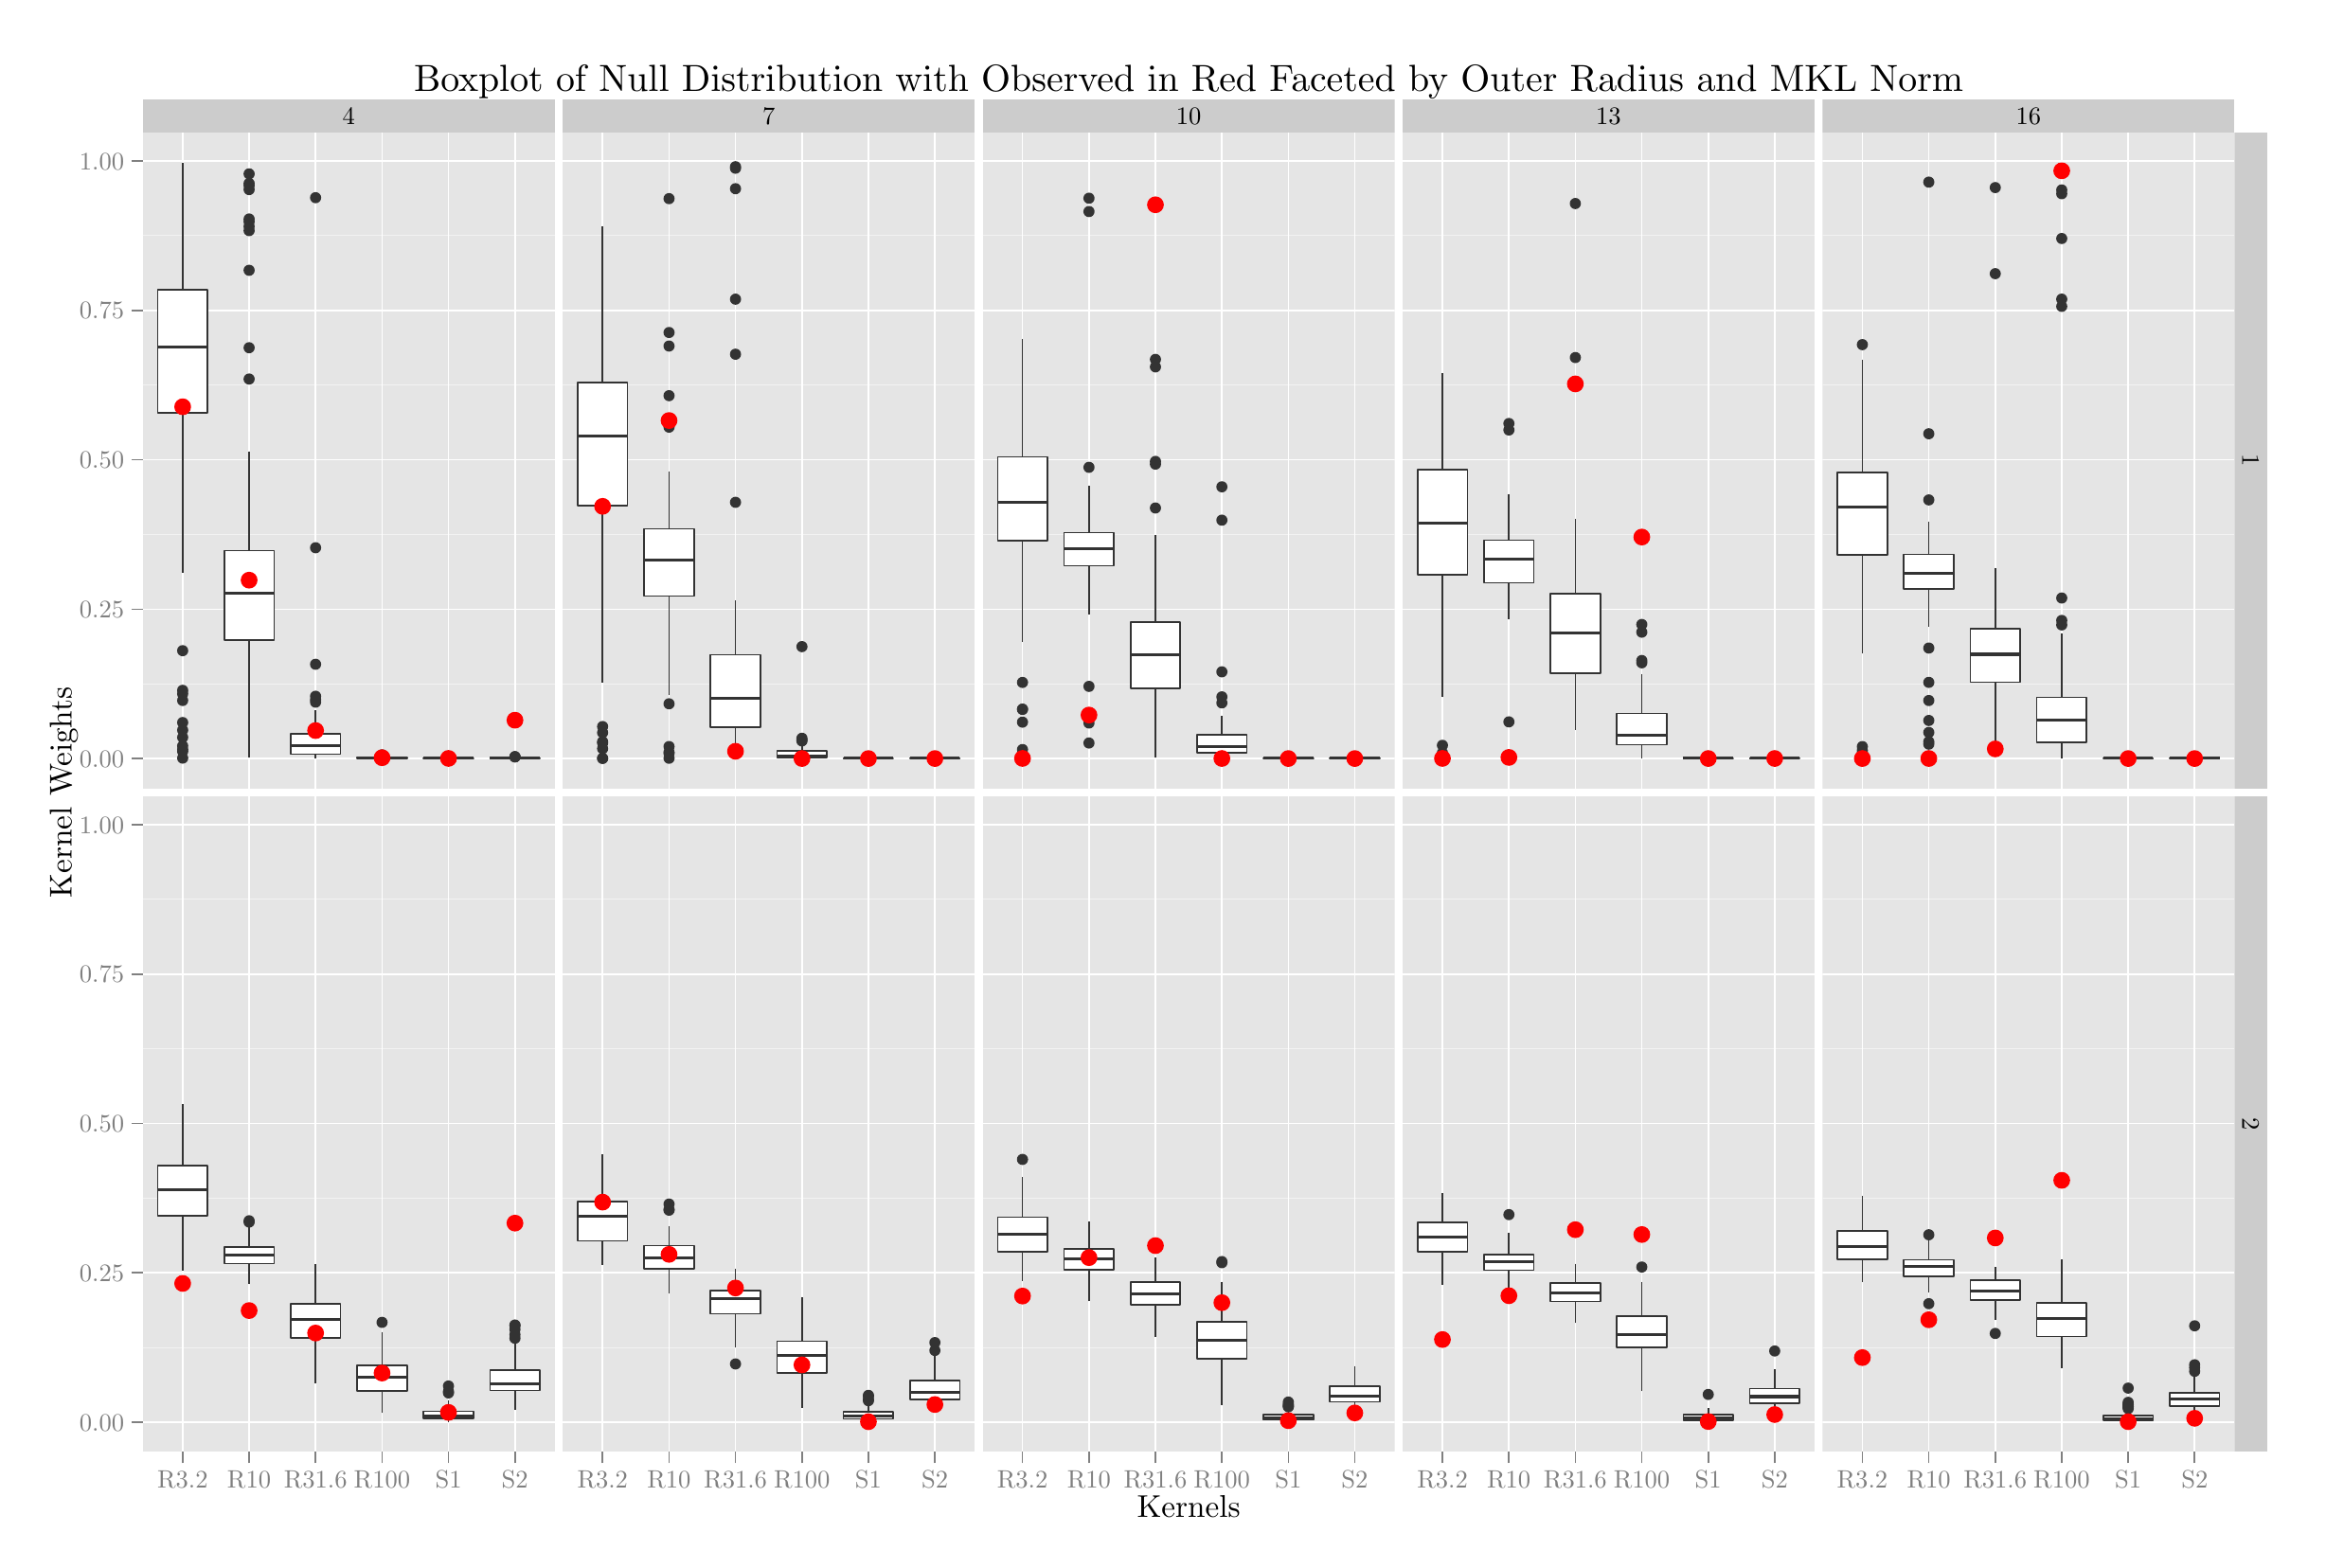
\begin{tikzpicture}[x=1pt,y=1pt]
\definecolor[named]{fillColor}{rgb}{1.00,1.00,1.00}
\path[use as bounding box,fill=fillColor,fill opacity=0.00] (0,0) rectangle (867.24,578.16);
\begin{scope}
\path[clip] (  0.00,  0.00) rectangle (867.24,578.16);
\definecolor[named]{drawColor}{rgb}{1.00,1.00,1.00}
\definecolor[named]{fillColor}{rgb}{1.00,1.00,1.00}

\path[draw=drawColor,line width= 0.6pt,line join=round,line cap=round,fill=fillColor] ( -0.00,  0.00) rectangle (867.24,578.16);
\end{scope}
\begin{scope}
\path[clip] ( 44.49,537.54) rectangle (201.69,550.17);
\definecolor[named]{fillColor}{rgb}{0.80,0.80,0.80}

\path[fill=fillColor] ( 44.49,537.54) rectangle (201.69,550.17);
\definecolor[named]{drawColor}{rgb}{0.00,0.00,0.00}

\node[text=drawColor,anchor=base,inner sep=0pt, outer sep=0pt, scale=  0.96] at (123.09,540.55) {4};
\end{scope}
\begin{scope}
\path[clip] (204.70,537.54) rectangle (361.91,550.17);
\definecolor[named]{fillColor}{rgb}{0.80,0.80,0.80}

\path[fill=fillColor] (204.70,537.54) rectangle (361.91,550.17);
\definecolor[named]{drawColor}{rgb}{0.00,0.00,0.00}

\node[text=drawColor,anchor=base,inner sep=0pt, outer sep=0pt, scale=  0.96] at (283.31,540.55) {7};
\end{scope}
\begin{scope}
\path[clip] (364.92,537.54) rectangle (522.13,550.17);
\definecolor[named]{fillColor}{rgb}{0.80,0.80,0.80}

\path[fill=fillColor] (364.92,537.54) rectangle (522.13,550.17);
\definecolor[named]{drawColor}{rgb}{0.00,0.00,0.00}

\node[text=drawColor,anchor=base,inner sep=0pt, outer sep=0pt, scale=  0.96] at (443.52,540.55) {10};
\end{scope}
\begin{scope}
\path[clip] (525.14,537.54) rectangle (682.34,550.17);
\definecolor[named]{fillColor}{rgb}{0.80,0.80,0.80}

\path[fill=fillColor] (525.14,537.54) rectangle (682.34,550.17);
\definecolor[named]{drawColor}{rgb}{0.00,0.00,0.00}

\node[text=drawColor,anchor=base,inner sep=0pt, outer sep=0pt, scale=  0.96] at (603.74,540.55) {13};
\end{scope}
\begin{scope}
\path[clip] (685.35,537.54) rectangle (842.56,550.17);
\definecolor[named]{fillColor}{rgb}{0.80,0.80,0.80}

\path[fill=fillColor] (685.35,537.54) rectangle (842.56,550.17);
\definecolor[named]{drawColor}{rgb}{0.00,0.00,0.00}

\node[text=drawColor,anchor=base,inner sep=0pt, outer sep=0pt, scale=  0.96] at (763.96,540.55) {16};
\end{scope}
\begin{scope}
\path[clip] ( 44.49,287.29) rectangle (201.69,537.54);
\definecolor[named]{fillColor}{rgb}{0.90,0.90,0.90}

\path[fill=fillColor] ( 44.49,287.29) rectangle (201.69,537.54);
\definecolor[named]{drawColor}{rgb}{0.95,0.95,0.95}

\path[draw=drawColor,line width= 0.3pt,line join=round] ( 44.49,327.17) --
	(201.69,327.17);

\path[draw=drawColor,line width= 0.3pt,line join=round] ( 44.49,384.18) --
	(201.69,384.18);

\path[draw=drawColor,line width= 0.3pt,line join=round] ( 44.49,441.20) --
	(201.69,441.20);

\path[draw=drawColor,line width= 0.3pt,line join=round] ( 44.49,498.21) --
	(201.69,498.21);
\definecolor[named]{drawColor}{rgb}{1.00,1.00,1.00}

\path[draw=drawColor,line width= 0.6pt,line join=round] ( 44.49,298.67) --
	(201.69,298.67);

\path[draw=drawColor,line width= 0.6pt,line join=round] ( 44.49,355.68) --
	(201.69,355.68);

\path[draw=drawColor,line width= 0.6pt,line join=round] ( 44.49,412.69) --
	(201.69,412.69);

\path[draw=drawColor,line width= 0.6pt,line join=round] ( 44.49,469.70) --
	(201.69,469.70);

\path[draw=drawColor,line width= 0.6pt,line join=round] ( 44.49,526.72) --
	(201.69,526.72);

\path[draw=drawColor,line width= 0.6pt,line join=round] ( 59.70,287.29) --
	( 59.70,537.54);

\path[draw=drawColor,line width= 0.6pt,line join=round] ( 85.05,287.29) --
	( 85.05,537.54);

\path[draw=drawColor,line width= 0.6pt,line join=round] (110.41,287.29) --
	(110.41,537.54);

\path[draw=drawColor,line width= 0.6pt,line join=round] (135.77,287.29) --
	(135.77,537.54);

\path[draw=drawColor,line width= 0.6pt,line join=round] (161.12,287.29) --
	(161.12,537.54);

\path[draw=drawColor,line width= 0.6pt,line join=round] (186.48,287.29) --
	(186.48,537.54);
\definecolor[named]{fillColor}{rgb}{0.20,0.20,0.20}

\path[fill=fillColor] ( 59.70,301.39) circle (  2.13);

\path[fill=fillColor] ( 59.70,320.83) circle (  2.13);

\path[fill=fillColor] ( 59.70,309.52) circle (  2.13);

\path[fill=fillColor] ( 59.70,312.41) circle (  2.13);

\path[fill=fillColor] ( 59.70,324.70) circle (  2.13);

\path[fill=fillColor] ( 59.70,303.50) circle (  2.13);

\path[fill=fillColor] ( 59.70,302.12) circle (  2.13);

\path[fill=fillColor] ( 59.70,323.35) circle (  2.13);

\path[fill=fillColor] ( 59.70,339.84) circle (  2.13);

\path[fill=fillColor] ( 59.70,306.75) circle (  2.13);

\path[fill=fillColor] ( 59.70,298.84) circle (  2.13);
\definecolor[named]{drawColor}{rgb}{0.20,0.20,0.20}

\path[draw=drawColor,line width= 0.6pt,line join=round,fill=fillColor] ( 59.70,477.67) -- ( 59.70,526.17);

\path[draw=drawColor,line width= 0.6pt,line join=round,fill=fillColor] ( 59.70,430.69) -- ( 59.70,369.63);
\definecolor[named]{fillColor}{rgb}{1.00,1.00,1.00}

\path[draw=drawColor,line width= 0.6pt,line join=round,line cap=round,fill=fillColor] ( 50.19,477.67) --
	( 50.19,430.69) --
	( 69.21,430.69) --
	( 69.21,477.67) --
	( 50.19,477.67) --
	cycle;
\definecolor[named]{fillColor}{rgb}{0.20,0.20,0.20}

\path[draw=drawColor,line width= 1.1pt,line join=round,fill=fillColor] ( 50.19,455.68) -- ( 69.21,455.68);

\path[fill=fillColor] ( 85.05,443.51) circle (  2.13);

\path[fill=fillColor] ( 85.05,503.57) circle (  2.13);

\path[fill=fillColor] ( 85.05,515.80) circle (  2.13);

\path[fill=fillColor] ( 85.05,504.58) circle (  2.13);

\path[fill=fillColor] ( 85.05,500.14) circle (  2.13);

\path[fill=fillColor] ( 85.05,521.79) circle (  2.13);

\path[fill=fillColor] ( 85.05,517.38) circle (  2.13);

\path[fill=fillColor] ( 85.05,501.71) circle (  2.13);

\path[fill=fillColor] ( 85.05,485.00) circle (  2.13);

\path[fill=fillColor] ( 85.05,518.17) circle (  2.13);

\path[fill=fillColor] ( 85.05,455.45) circle (  2.13);

\path[draw=drawColor,line width= 0.6pt,line join=round,fill=fillColor] ( 85.05,378.02) -- ( 85.05,415.89);

\path[draw=drawColor,line width= 0.6pt,line join=round,fill=fillColor] ( 85.05,343.91) -- ( 85.05,299.20);
\definecolor[named]{fillColor}{rgb}{1.00,1.00,1.00}

\path[draw=drawColor,line width= 0.6pt,line join=round,line cap=round,fill=fillColor] ( 75.55,378.02) --
	( 75.55,343.91) --
	( 94.56,343.91) --
	( 94.56,378.02) --
	( 75.55,378.02) --
	cycle;
\definecolor[named]{fillColor}{rgb}{0.20,0.20,0.20}

\path[draw=drawColor,line width= 1.1pt,line join=round,fill=fillColor] ( 75.55,361.64) -- ( 94.56,361.64);

\path[fill=fillColor] (110.41,320.19) circle (  2.13);

\path[fill=fillColor] (110.41,379.12) circle (  2.13);

\path[fill=fillColor] (110.41,322.45) circle (  2.13);

\path[fill=fillColor] (110.41,321.11) circle (  2.13);

\path[fill=fillColor] (110.41,512.71) circle (  2.13);

\path[fill=fillColor] (110.41,334.65) circle (  2.13);

\path[draw=drawColor,line width= 0.6pt,line join=round,fill=fillColor] (110.41,308.03) -- (110.41,317.12);

\path[draw=drawColor,line width= 0.6pt,line join=round,fill=fillColor] (110.41,300.34) -- (110.41,298.67);
\definecolor[named]{fillColor}{rgb}{1.00,1.00,1.00}

\path[draw=drawColor,line width= 0.6pt,line join=round,line cap=round,fill=fillColor] (100.90,308.03) --
	(100.90,300.34) --
	(119.92,300.34) --
	(119.92,308.03) --
	(100.90,308.03) --
	cycle;
\definecolor[named]{fillColor}{rgb}{0.20,0.20,0.20}

\path[draw=drawColor,line width= 1.1pt,line join=round,fill=fillColor] (100.90,303.42) -- (119.92,303.42);

\path[fill=fillColor] (135.77,299.50) circle (  2.13);

\path[fill=fillColor] (135.77,299.57) circle (  2.13);

\path[fill=fillColor] (135.77,299.61) circle (  2.13);

\path[fill=fillColor] (135.77,299.49) circle (  2.13);

\path[fill=fillColor] (135.77,300.09) circle (  2.13);

\path[draw=drawColor,line width= 0.6pt,line join=round,fill=fillColor] (135.77,299.02) -- (135.77,299.42);

\path[draw=drawColor,line width= 0.6pt,line join=round,fill=fillColor] (135.77,298.75) -- (135.77,298.67);
\definecolor[named]{fillColor}{rgb}{1.00,1.00,1.00}

\path[draw=drawColor,line width= 0.6pt,line join=round,line cap=round,fill=fillColor] (126.26,299.02) --
	(126.26,298.75) --
	(145.27,298.75) --
	(145.27,299.02) --
	(126.26,299.02) --
	cycle;
\definecolor[named]{fillColor}{rgb}{0.20,0.20,0.20}

\path[draw=drawColor,line width= 1.1pt,line join=round,fill=fillColor] (126.26,298.89) -- (145.27,298.89);

\path[fill=fillColor] (161.12,299.03) circle (  2.13);

\path[draw=drawColor,line width= 0.6pt,line join=round,fill=fillColor] (161.12,298.82) -- (161.12,298.97);

\path[draw=drawColor,line width= 0.6pt,line join=round,fill=fillColor] (161.12,298.69) -- (161.12,298.67);
\definecolor[named]{fillColor}{rgb}{1.00,1.00,1.00}

\path[draw=drawColor,line width= 0.6pt,line join=round,line cap=round,fill=fillColor] (151.61,298.82) --
	(151.61,298.69) --
	(170.63,298.69) --
	(170.63,298.82) --
	(151.61,298.82) --
	cycle;
\definecolor[named]{fillColor}{rgb}{0.20,0.20,0.20}

\path[draw=drawColor,line width= 1.1pt,line join=round,fill=fillColor] (151.61,298.75) -- (170.63,298.75);

\path[fill=fillColor] (186.48,299.30) circle (  2.13);

\path[fill=fillColor] (186.48,299.32) circle (  2.13);

\path[fill=fillColor] (186.48,299.41) circle (  2.13);

\path[draw=drawColor,line width= 0.6pt,line join=round,fill=fillColor] (186.48,298.92) -- (186.48,299.24);

\path[draw=drawColor,line width= 0.6pt,line join=round,fill=fillColor] (186.48,298.70) -- (186.48,298.67);
\definecolor[named]{fillColor}{rgb}{1.00,1.00,1.00}

\path[draw=drawColor,line width= 0.6pt,line join=round,line cap=round,fill=fillColor] (176.97,298.92) --
	(176.97,298.70) --
	(195.99,298.70) --
	(195.99,298.92) --
	(176.97,298.92) --
	cycle;
\definecolor[named]{fillColor}{rgb}{0.20,0.20,0.20}

\path[draw=drawColor,line width= 1.1pt,line join=round,fill=fillColor] (176.97,298.83) -- (195.99,298.83);
\definecolor[named]{fillColor}{rgb}{1.00,0.00,0.00}

\path[fill=fillColor] ( 59.70,432.91) circle (  3.20);

\path[fill=fillColor] ( 85.05,366.75) circle (  3.20);

\path[fill=fillColor] (110.41,309.35) circle (  3.20);

\path[fill=fillColor] (135.77,298.99) circle (  3.20);

\path[fill=fillColor] (161.12,298.72) circle (  3.20);

\path[fill=fillColor] (186.48,313.31) circle (  3.20);
\end{scope}
\begin{scope}
\path[clip] ( 44.49, 34.03) rectangle (201.69,284.28);
\definecolor[named]{fillColor}{rgb}{0.90,0.90,0.90}

\path[fill=fillColor] ( 44.49, 34.03) rectangle (201.69,284.28);
\definecolor[named]{drawColor}{rgb}{0.95,0.95,0.95}

\path[draw=drawColor,line width= 0.3pt,line join=round] ( 44.49, 73.91) --
	(201.69, 73.91);

\path[draw=drawColor,line width= 0.3pt,line join=round] ( 44.49,130.93) --
	(201.69,130.93);

\path[draw=drawColor,line width= 0.3pt,line join=round] ( 44.49,187.94) --
	(201.69,187.94);

\path[draw=drawColor,line width= 0.3pt,line join=round] ( 44.49,244.95) --
	(201.69,244.95);
\definecolor[named]{drawColor}{rgb}{1.00,1.00,1.00}

\path[draw=drawColor,line width= 0.6pt,line join=round] ( 44.49, 45.41) --
	(201.69, 45.41);

\path[draw=drawColor,line width= 0.6pt,line join=round] ( 44.49,102.42) --
	(201.69,102.42);

\path[draw=drawColor,line width= 0.6pt,line join=round] ( 44.49,159.43) --
	(201.69,159.43);

\path[draw=drawColor,line width= 0.6pt,line join=round] ( 44.49,216.44) --
	(201.69,216.44);

\path[draw=drawColor,line width= 0.6pt,line join=round] ( 44.49,273.46) --
	(201.69,273.46);

\path[draw=drawColor,line width= 0.6pt,line join=round] ( 59.70, 34.03) --
	( 59.70,284.28);

\path[draw=drawColor,line width= 0.6pt,line join=round] ( 85.05, 34.03) --
	( 85.05,284.28);

\path[draw=drawColor,line width= 0.6pt,line join=round] (110.41, 34.03) --
	(110.41,284.28);

\path[draw=drawColor,line width= 0.6pt,line join=round] (135.77, 34.03) --
	(135.77,284.28);

\path[draw=drawColor,line width= 0.6pt,line join=round] (161.12, 34.03) --
	(161.12,284.28);

\path[draw=drawColor,line width= 0.6pt,line join=round] (186.48, 34.03) --
	(186.48,284.28);
\definecolor[named]{drawColor}{rgb}{0.20,0.20,0.20}
\definecolor[named]{fillColor}{rgb}{0.20,0.20,0.20}

\path[draw=drawColor,line width= 0.6pt,line join=round,fill=fillColor] ( 59.70,143.26) -- ( 59.70,166.78);

\path[draw=drawColor,line width= 0.6pt,line join=round,fill=fillColor] ( 59.70,124.07) -- ( 59.70,103.19);
\definecolor[named]{fillColor}{rgb}{1.00,1.00,1.00}

\path[draw=drawColor,line width= 0.6pt,line join=round,line cap=round,fill=fillColor] ( 50.19,143.26) --
	( 50.19,124.07) --
	( 69.21,124.07) --
	( 69.21,143.26) --
	( 50.19,143.26) --
	cycle;
\definecolor[named]{fillColor}{rgb}{0.20,0.20,0.20}

\path[draw=drawColor,line width= 1.1pt,line join=round,fill=fillColor] ( 50.19,133.95) -- ( 69.21,133.95);

\path[fill=fillColor] ( 85.05,121.78) circle (  2.13);

\path[fill=fillColor] ( 85.05,122.28) circle (  2.13);

\path[draw=drawColor,line width= 0.6pt,line join=round,fill=fillColor] ( 85.05,112.19) -- ( 85.05,121.48);

\path[draw=drawColor,line width= 0.6pt,line join=round,fill=fillColor] ( 85.05,105.96) -- ( 85.05, 97.99);
\definecolor[named]{fillColor}{rgb}{1.00,1.00,1.00}

\path[draw=drawColor,line width= 0.6pt,line join=round,line cap=round,fill=fillColor] ( 75.55,112.19) --
	( 75.55,105.96) --
	( 94.56,105.96) --
	( 94.56,112.19) --
	( 75.55,112.19) --
	cycle;
\definecolor[named]{fillColor}{rgb}{0.20,0.20,0.20}

\path[draw=drawColor,line width= 1.1pt,line join=round,fill=fillColor] ( 75.55,109.29) -- ( 94.56,109.29);

\path[draw=drawColor,line width= 0.6pt,line join=round,fill=fillColor] (110.41, 90.46) -- (110.41,105.75);

\path[draw=drawColor,line width= 0.6pt,line join=round,fill=fillColor] (110.41, 77.48) -- (110.41, 60.37);
\definecolor[named]{fillColor}{rgb}{1.00,1.00,1.00}

\path[draw=drawColor,line width= 0.6pt,line join=round,line cap=round,fill=fillColor] (100.90, 90.46) --
	(100.90, 77.48) --
	(119.92, 77.48) --
	(119.92, 90.46) --
	(100.90, 90.46) --
	cycle;
\definecolor[named]{fillColor}{rgb}{0.20,0.20,0.20}

\path[draw=drawColor,line width= 1.1pt,line join=round,fill=fillColor] (100.90, 84.46) -- (119.92, 84.46);

\path[fill=fillColor] (135.77, 83.50) circle (  2.13);

\path[draw=drawColor,line width= 0.6pt,line join=round,fill=fillColor] (135.77, 67.15) -- (135.77, 79.90);

\path[draw=drawColor,line width= 0.6pt,line join=round,fill=fillColor] (135.77, 57.32) -- (135.77, 48.89);
\definecolor[named]{fillColor}{rgb}{1.00,1.00,1.00}

\path[draw=drawColor,line width= 0.6pt,line join=round,line cap=round,fill=fillColor] (126.26, 67.15) --
	(126.26, 57.32) --
	(145.27, 57.32) --
	(145.27, 67.15) --
	(126.26, 67.15) --
	cycle;
\definecolor[named]{fillColor}{rgb}{0.20,0.20,0.20}

\path[draw=drawColor,line width= 1.1pt,line join=round,fill=fillColor] (126.26, 62.69) -- (145.27, 62.69);

\path[fill=fillColor] (161.12, 59.21) circle (  2.13);

\path[fill=fillColor] (161.12, 56.58) circle (  2.13);

\path[fill=fillColor] (161.12, 57.09) circle (  2.13);

\path[draw=drawColor,line width= 0.6pt,line join=round,fill=fillColor] (161.12, 49.62) -- (161.12, 53.58);

\path[draw=drawColor,line width= 0.6pt,line join=round,fill=fillColor] (161.12, 46.75) -- (161.12, 45.54);
\definecolor[named]{fillColor}{rgb}{1.00,1.00,1.00}

\path[draw=drawColor,line width= 0.6pt,line join=round,line cap=round,fill=fillColor] (151.61, 49.62) --
	(151.61, 46.75) --
	(170.63, 46.75) --
	(170.63, 49.62) --
	(151.61, 49.62) --
	cycle;
\definecolor[named]{fillColor}{rgb}{0.20,0.20,0.20}

\path[draw=drawColor,line width= 1.1pt,line join=round,fill=fillColor] (151.61, 47.93) -- (170.63, 47.93);

\path[fill=fillColor] (186.48, 80.82) circle (  2.13);

\path[fill=fillColor] (186.48, 77.44) circle (  2.13);

\path[fill=fillColor] (186.48, 82.32) circle (  2.13);

\path[fill=fillColor] (186.48, 82.49) circle (  2.13);

\path[fill=fillColor] (186.48, 78.84) circle (  2.13);

\path[draw=drawColor,line width= 0.6pt,line join=round,fill=fillColor] (186.48, 65.40) -- (186.48, 76.86);

\path[draw=drawColor,line width= 0.6pt,line join=round,fill=fillColor] (186.48, 57.52) -- (186.48, 50.20);
\definecolor[named]{fillColor}{rgb}{1.00,1.00,1.00}

\path[draw=drawColor,line width= 0.6pt,line join=round,line cap=round,fill=fillColor] (176.97, 65.40) --
	(176.97, 57.52) --
	(195.99, 57.52) --
	(195.99, 65.40) --
	(176.97, 65.40) --
	cycle;
\definecolor[named]{fillColor}{rgb}{0.20,0.20,0.20}

\path[draw=drawColor,line width= 1.1pt,line join=round,fill=fillColor] (176.97, 59.91) -- (195.99, 59.91);
\definecolor[named]{fillColor}{rgb}{1.00,0.00,0.00}

\path[fill=fillColor] ( 59.70, 98.36) circle (  3.20);

\path[fill=fillColor] ( 85.05, 88.01) circle (  3.20);

\path[fill=fillColor] (110.41, 79.43) circle (  3.20);

\path[fill=fillColor] (135.77, 64.16) circle (  3.20);

\path[fill=fillColor] (161.12, 49.14) circle (  3.20);

\path[fill=fillColor] (186.48,121.38) circle (  3.20);
\end{scope}
\begin{scope}
\path[clip] (204.70,287.29) rectangle (361.91,537.54);
\definecolor[named]{fillColor}{rgb}{0.90,0.90,0.90}

\path[fill=fillColor] (204.70,287.29) rectangle (361.91,537.54);
\definecolor[named]{drawColor}{rgb}{0.95,0.95,0.95}

\path[draw=drawColor,line width= 0.3pt,line join=round] (204.70,327.17) --
	(361.91,327.17);

\path[draw=drawColor,line width= 0.3pt,line join=round] (204.70,384.18) --
	(361.91,384.18);

\path[draw=drawColor,line width= 0.3pt,line join=round] (204.70,441.20) --
	(361.91,441.20);

\path[draw=drawColor,line width= 0.3pt,line join=round] (204.70,498.21) --
	(361.91,498.21);
\definecolor[named]{drawColor}{rgb}{1.00,1.00,1.00}

\path[draw=drawColor,line width= 0.6pt,line join=round] (204.70,298.67) --
	(361.91,298.67);

\path[draw=drawColor,line width= 0.6pt,line join=round] (204.70,355.68) --
	(361.91,355.68);

\path[draw=drawColor,line width= 0.6pt,line join=round] (204.70,412.69) --
	(361.91,412.69);

\path[draw=drawColor,line width= 0.6pt,line join=round] (204.70,469.70) --
	(361.91,469.70);

\path[draw=drawColor,line width= 0.6pt,line join=round] (204.70,526.72) --
	(361.91,526.72);

\path[draw=drawColor,line width= 0.6pt,line join=round] (219.92,287.29) --
	(219.92,537.54);

\path[draw=drawColor,line width= 0.6pt,line join=round] (245.27,287.29) --
	(245.27,537.54);

\path[draw=drawColor,line width= 0.6pt,line join=round] (270.63,287.29) --
	(270.63,537.54);

\path[draw=drawColor,line width= 0.6pt,line join=round] (295.98,287.29) --
	(295.98,537.54);

\path[draw=drawColor,line width= 0.6pt,line join=round] (321.34,287.29) --
	(321.34,537.54);

\path[draw=drawColor,line width= 0.6pt,line join=round] (346.70,287.29) --
	(346.70,537.54);
\definecolor[named]{fillColor}{rgb}{0.20,0.20,0.20}

\path[fill=fillColor] (219.92,310.88) circle (  2.13);

\path[fill=fillColor] (219.92,305.11) circle (  2.13);

\path[fill=fillColor] (219.92,298.74) circle (  2.13);

\path[fill=fillColor] (219.92,302.43) circle (  2.13);

\path[fill=fillColor] (219.92,298.76) circle (  2.13);

\path[fill=fillColor] (219.92,304.61) circle (  2.13);

\path[fill=fillColor] (219.92,308.55) circle (  2.13);
\definecolor[named]{drawColor}{rgb}{0.20,0.20,0.20}

\path[draw=drawColor,line width= 0.6pt,line join=round,fill=fillColor] (219.92,442.18) -- (219.92,501.86);

\path[draw=drawColor,line width= 0.6pt,line join=round,fill=fillColor] (219.92,395.30) -- (219.92,327.80);
\definecolor[named]{fillColor}{rgb}{1.00,1.00,1.00}

\path[draw=drawColor,line width= 0.6pt,line join=round,line cap=round,fill=fillColor] (210.41,442.18) --
	(210.41,395.30) --
	(229.42,395.30) --
	(229.42,442.18) --
	(210.41,442.18) --
	cycle;
\definecolor[named]{fillColor}{rgb}{0.20,0.20,0.20}

\path[draw=drawColor,line width= 1.1pt,line join=round,fill=fillColor] (210.41,421.58) -- (229.42,421.58);

\path[fill=fillColor] (245.27,512.35) circle (  2.13);

\path[fill=fillColor] (245.27,456.09) circle (  2.13);

\path[fill=fillColor] (245.27,437.15) circle (  2.13);

\path[fill=fillColor] (245.27,461.26) circle (  2.13);

\path[fill=fillColor] (245.27,300.63) circle (  2.13);

\path[fill=fillColor] (245.27,425.13) circle (  2.13);

\path[fill=fillColor] (245.27,301.08) circle (  2.13);

\path[fill=fillColor] (245.27,319.57) circle (  2.13);

\path[fill=fillColor] (245.27,303.25) circle (  2.13);

\path[fill=fillColor] (245.27,298.78) circle (  2.13);

\path[draw=drawColor,line width= 0.6pt,line join=round,fill=fillColor] (245.27,386.32) -- (245.27,408.28);

\path[draw=drawColor,line width= 0.6pt,line join=round,fill=fillColor] (245.27,360.73) -- (245.27,322.89);
\definecolor[named]{fillColor}{rgb}{1.00,1.00,1.00}

\path[draw=drawColor,line width= 0.6pt,line join=round,line cap=round,fill=fillColor] (235.76,386.32) --
	(235.76,360.73) --
	(254.78,360.73) --
	(254.78,386.32) --
	(235.76,386.32) --
	cycle;
\definecolor[named]{fillColor}{rgb}{0.20,0.20,0.20}

\path[draw=drawColor,line width= 1.1pt,line join=round,fill=fillColor] (235.76,374.57) -- (254.78,374.57);

\path[fill=fillColor] (270.63,524.53) circle (  2.13);

\path[fill=fillColor] (270.63,396.46) circle (  2.13);

\path[fill=fillColor] (270.63,452.97) circle (  2.13);

\path[fill=fillColor] (270.63,523.95) circle (  2.13);

\path[fill=fillColor] (270.63,516.14) circle (  2.13);

\path[fill=fillColor] (270.63,473.98) circle (  2.13);

\path[draw=drawColor,line width= 0.6pt,line join=round,fill=fillColor] (270.63,338.31) -- (270.63,359.02);

\path[draw=drawColor,line width= 0.6pt,line join=round,fill=fillColor] (270.63,310.55) -- (270.63,298.70);
\definecolor[named]{fillColor}{rgb}{1.00,1.00,1.00}

\path[draw=drawColor,line width= 0.6pt,line join=round,line cap=round,fill=fillColor] (261.12,338.31) --
	(261.12,310.55) --
	(280.14,310.55) --
	(280.14,338.31) --
	(261.12,338.31) --
	cycle;
\definecolor[named]{fillColor}{rgb}{0.20,0.20,0.20}

\path[draw=drawColor,line width= 1.1pt,line join=round,fill=fillColor] (261.12,321.70) -- (280.14,321.70);

\path[fill=fillColor] (295.98,305.39) circle (  2.13);

\path[fill=fillColor] (295.98,306.41) circle (  2.13);

\path[fill=fillColor] (295.98,305.75) circle (  2.13);

\path[fill=fillColor] (295.98,341.38) circle (  2.13);

\path[draw=drawColor,line width= 0.6pt,line join=round,fill=fillColor] (295.98,301.49) -- (295.98,304.49);

\path[draw=drawColor,line width= 0.6pt,line join=round,fill=fillColor] (295.98,299.16) -- (295.98,298.68);
\definecolor[named]{fillColor}{rgb}{1.00,1.00,1.00}

\path[draw=drawColor,line width= 0.6pt,line join=round,line cap=round,fill=fillColor] (286.48,301.49) --
	(286.48,299.16) --
	(305.49,299.16) --
	(305.49,301.49) --
	(286.48,301.49) --
	cycle;
\definecolor[named]{fillColor}{rgb}{0.20,0.20,0.20}

\path[draw=drawColor,line width= 1.1pt,line join=round,fill=fillColor] (286.48,299.63) -- (305.49,299.63);

\path[draw=drawColor,line width= 0.6pt,line join=round,fill=fillColor] (321.34,298.81) -- (321.34,298.89);

\path[draw=drawColor,line width= 0.6pt,line join=round,fill=fillColor] (321.34,298.72) -- (321.34,298.67);
\definecolor[named]{fillColor}{rgb}{1.00,1.00,1.00}

\path[draw=drawColor,line width= 0.6pt,line join=round,line cap=round,fill=fillColor] (311.83,298.81) --
	(311.83,298.72) --
	(330.85,298.72) --
	(330.85,298.81) --
	(311.83,298.81) --
	cycle;
\definecolor[named]{fillColor}{rgb}{0.20,0.20,0.20}

\path[draw=drawColor,line width= 1.1pt,line join=round,fill=fillColor] (311.83,298.77) -- (330.85,298.77);

\path[fill=fillColor] (346.70,299.11) circle (  2.13);

\path[draw=drawColor,line width= 0.6pt,line join=round,fill=fillColor] (346.70,298.89) -- (346.70,299.02);

\path[draw=drawColor,line width= 0.6pt,line join=round,fill=fillColor] (346.70,298.77) -- (346.70,298.67);
\definecolor[named]{fillColor}{rgb}{1.00,1.00,1.00}

\path[draw=drawColor,line width= 0.6pt,line join=round,line cap=round,fill=fillColor] (337.19,298.89) --
	(337.19,298.77) --
	(356.20,298.77) --
	(356.20,298.89) --
	(337.19,298.89) --
	cycle;
\definecolor[named]{fillColor}{rgb}{0.20,0.20,0.20}

\path[draw=drawColor,line width= 1.1pt,line join=round,fill=fillColor] (337.19,298.84) -- (356.20,298.84);
\definecolor[named]{fillColor}{rgb}{1.00,0.00,0.00}

\path[fill=fillColor] (219.92,394.92) circle (  3.20);

\path[fill=fillColor] (245.27,427.67) circle (  3.20);

\path[fill=fillColor] (270.63,301.44) circle (  3.20);

\path[fill=fillColor] (295.98,298.68) circle (  3.20);

\path[fill=fillColor] (321.34,298.67) circle (  3.20);

\path[fill=fillColor] (346.70,298.67) circle (  3.20);
\end{scope}
\begin{scope}
\path[clip] (204.70, 34.03) rectangle (361.91,284.28);
\definecolor[named]{fillColor}{rgb}{0.90,0.90,0.90}

\path[fill=fillColor] (204.70, 34.03) rectangle (361.91,284.28);
\definecolor[named]{drawColor}{rgb}{0.95,0.95,0.95}

\path[draw=drawColor,line width= 0.3pt,line join=round] (204.70, 73.91) --
	(361.91, 73.91);

\path[draw=drawColor,line width= 0.3pt,line join=round] (204.70,130.93) --
	(361.91,130.93);

\path[draw=drawColor,line width= 0.3pt,line join=round] (204.70,187.94) --
	(361.91,187.94);

\path[draw=drawColor,line width= 0.3pt,line join=round] (204.70,244.95) --
	(361.91,244.95);
\definecolor[named]{drawColor}{rgb}{1.00,1.00,1.00}

\path[draw=drawColor,line width= 0.6pt,line join=round] (204.70, 45.41) --
	(361.91, 45.41);

\path[draw=drawColor,line width= 0.6pt,line join=round] (204.70,102.42) --
	(361.91,102.42);

\path[draw=drawColor,line width= 0.6pt,line join=round] (204.70,159.43) --
	(361.91,159.43);

\path[draw=drawColor,line width= 0.6pt,line join=round] (204.70,216.44) --
	(361.91,216.44);

\path[draw=drawColor,line width= 0.6pt,line join=round] (204.70,273.46) --
	(361.91,273.46);

\path[draw=drawColor,line width= 0.6pt,line join=round] (219.92, 34.03) --
	(219.92,284.28);

\path[draw=drawColor,line width= 0.6pt,line join=round] (245.27, 34.03) --
	(245.27,284.28);

\path[draw=drawColor,line width= 0.6pt,line join=round] (270.63, 34.03) --
	(270.63,284.28);

\path[draw=drawColor,line width= 0.6pt,line join=round] (295.98, 34.03) --
	(295.98,284.28);

\path[draw=drawColor,line width= 0.6pt,line join=round] (321.34, 34.03) --
	(321.34,284.28);

\path[draw=drawColor,line width= 0.6pt,line join=round] (346.70, 34.03) --
	(346.70,284.28);
\definecolor[named]{drawColor}{rgb}{0.20,0.20,0.20}
\definecolor[named]{fillColor}{rgb}{0.20,0.20,0.20}

\path[draw=drawColor,line width= 0.6pt,line join=round,fill=fillColor] (219.92,129.62) -- (219.92,147.65);

\path[draw=drawColor,line width= 0.6pt,line join=round,fill=fillColor] (219.92,114.63) -- (219.92,105.55);
\definecolor[named]{fillColor}{rgb}{1.00,1.00,1.00}

\path[draw=drawColor,line width= 0.6pt,line join=round,line cap=round,fill=fillColor] (210.41,129.62) --
	(210.41,114.63) --
	(229.42,114.63) --
	(229.42,129.62) --
	(210.41,129.62) --
	cycle;
\definecolor[named]{fillColor}{rgb}{0.20,0.20,0.20}

\path[draw=drawColor,line width= 1.1pt,line join=round,fill=fillColor] (210.41,124.05) -- (229.42,124.05);

\path[fill=fillColor] (245.27,128.65) circle (  2.13);

\path[fill=fillColor] (245.27,126.31) circle (  2.13);

\path[fill=fillColor] (245.27,126.56) circle (  2.13);

\path[draw=drawColor,line width= 0.6pt,line join=round,fill=fillColor] (245.27,112.84) -- (245.27,120.26);

\path[draw=drawColor,line width= 0.6pt,line join=round,fill=fillColor] (245.27,104.02) -- (245.27, 94.45);
\definecolor[named]{fillColor}{rgb}{1.00,1.00,1.00}

\path[draw=drawColor,line width= 0.6pt,line join=round,line cap=round,fill=fillColor] (235.76,112.84) --
	(235.76,104.02) --
	(254.78,104.02) --
	(254.78,112.84) --
	(235.76,112.84) --
	cycle;
\definecolor[named]{fillColor}{rgb}{0.20,0.20,0.20}

\path[draw=drawColor,line width= 1.1pt,line join=round,fill=fillColor] (235.76,108.24) -- (254.78,108.24);

\path[fill=fillColor] (270.63, 67.64) circle (  2.13);

\path[draw=drawColor,line width= 0.6pt,line join=round,fill=fillColor] (270.63, 95.56) -- (270.63,103.93);

\path[draw=drawColor,line width= 0.6pt,line join=round,fill=fillColor] (270.63, 86.79) -- (270.63, 73.82);
\definecolor[named]{fillColor}{rgb}{1.00,1.00,1.00}

\path[draw=drawColor,line width= 0.6pt,line join=round,line cap=round,fill=fillColor] (261.12, 95.56) --
	(261.12, 86.79) --
	(280.14, 86.79) --
	(280.14, 95.56) --
	(261.12, 95.56) --
	cycle;
\definecolor[named]{fillColor}{rgb}{0.20,0.20,0.20}

\path[draw=drawColor,line width= 1.1pt,line join=round,fill=fillColor] (261.12, 92.55) -- (280.14, 92.55);

\path[draw=drawColor,line width= 0.6pt,line join=round,fill=fillColor] (295.98, 76.27) -- (295.98, 93.15);

\path[draw=drawColor,line width= 0.6pt,line join=round,fill=fillColor] (295.98, 64.23) -- (295.98, 50.99);
\definecolor[named]{fillColor}{rgb}{1.00,1.00,1.00}

\path[draw=drawColor,line width= 0.6pt,line join=round,line cap=round,fill=fillColor] (286.48, 76.27) --
	(286.48, 64.23) --
	(305.49, 64.23) --
	(305.49, 76.27) --
	(286.48, 76.27) --
	cycle;
\definecolor[named]{fillColor}{rgb}{0.20,0.20,0.20}

\path[draw=drawColor,line width= 1.1pt,line join=round,fill=fillColor] (286.48, 70.75) -- (305.49, 70.75);

\path[fill=fillColor] (321.34, 55.65) circle (  2.13);

\path[fill=fillColor] (321.34, 54.04) circle (  2.13);

\path[fill=fillColor] (321.34, 53.61) circle (  2.13);

\path[fill=fillColor] (321.34, 55.33) circle (  2.13);

\path[draw=drawColor,line width= 0.6pt,line join=round,fill=fillColor] (321.34, 49.42) -- (321.34, 52.88);

\path[draw=drawColor,line width= 0.6pt,line join=round,fill=fillColor] (321.34, 46.68) -- (321.34, 45.44);
\definecolor[named]{fillColor}{rgb}{1.00,1.00,1.00}

\path[draw=drawColor,line width= 0.6pt,line join=round,line cap=round,fill=fillColor] (311.83, 49.42) --
	(311.83, 46.68) --
	(330.85, 46.68) --
	(330.85, 49.42) --
	(311.83, 49.42) --
	cycle;
\definecolor[named]{fillColor}{rgb}{0.20,0.20,0.20}

\path[draw=drawColor,line width= 1.1pt,line join=round,fill=fillColor] (311.83, 47.72) -- (330.85, 47.72);

\path[fill=fillColor] (346.70, 75.79) circle (  2.13);

\path[fill=fillColor] (346.70, 72.78) circle (  2.13);

\path[draw=drawColor,line width= 0.6pt,line join=round,fill=fillColor] (346.70, 61.33) -- (346.70, 71.75);

\path[draw=drawColor,line width= 0.6pt,line join=round,fill=fillColor] (346.70, 54.11) -- (346.70, 50.73);
\definecolor[named]{fillColor}{rgb}{1.00,1.00,1.00}

\path[draw=drawColor,line width= 0.6pt,line join=round,line cap=round,fill=fillColor] (337.19, 61.33) --
	(337.19, 54.11) --
	(356.20, 54.11) --
	(356.20, 61.33) --
	(337.19, 61.33) --
	cycle;
\definecolor[named]{fillColor}{rgb}{0.20,0.20,0.20}

\path[draw=drawColor,line width= 1.1pt,line join=round,fill=fillColor] (337.19, 56.88) -- (356.20, 56.88);
\definecolor[named]{fillColor}{rgb}{1.00,0.00,0.00}

\path[fill=fillColor] (219.92,129.40) circle (  3.20);

\path[fill=fillColor] (245.27,109.45) circle (  3.20);

\path[fill=fillColor] (270.63, 96.62) circle (  3.20);

\path[fill=fillColor] (295.98, 67.28) circle (  3.20);

\path[fill=fillColor] (321.34, 45.59) circle (  3.20);

\path[fill=fillColor] (346.70, 52.15) circle (  3.20);
\end{scope}
\begin{scope}
\path[clip] (364.92,287.29) rectangle (522.13,537.54);
\definecolor[named]{fillColor}{rgb}{0.90,0.90,0.90}

\path[fill=fillColor] (364.92,287.29) rectangle (522.13,537.54);
\definecolor[named]{drawColor}{rgb}{0.95,0.95,0.95}

\path[draw=drawColor,line width= 0.3pt,line join=round] (364.92,327.17) --
	(522.13,327.17);

\path[draw=drawColor,line width= 0.3pt,line join=round] (364.92,384.18) --
	(522.13,384.18);

\path[draw=drawColor,line width= 0.3pt,line join=round] (364.92,441.20) --
	(522.13,441.20);

\path[draw=drawColor,line width= 0.3pt,line join=round] (364.92,498.21) --
	(522.13,498.21);
\definecolor[named]{drawColor}{rgb}{1.00,1.00,1.00}

\path[draw=drawColor,line width= 0.6pt,line join=round] (364.92,298.67) --
	(522.13,298.67);

\path[draw=drawColor,line width= 0.6pt,line join=round] (364.92,355.68) --
	(522.13,355.68);

\path[draw=drawColor,line width= 0.6pt,line join=round] (364.92,412.69) --
	(522.13,412.69);

\path[draw=drawColor,line width= 0.6pt,line join=round] (364.92,469.70) --
	(522.13,469.70);

\path[draw=drawColor,line width= 0.6pt,line join=round] (364.92,526.72) --
	(522.13,526.72);

\path[draw=drawColor,line width= 0.6pt,line join=round] (380.13,287.29) --
	(380.13,537.54);

\path[draw=drawColor,line width= 0.6pt,line join=round] (405.49,287.29) --
	(405.49,537.54);

\path[draw=drawColor,line width= 0.6pt,line join=round] (430.85,287.29) --
	(430.85,537.54);

\path[draw=drawColor,line width= 0.6pt,line join=round] (456.20,287.29) --
	(456.20,537.54);

\path[draw=drawColor,line width= 0.6pt,line join=round] (481.56,287.29) --
	(481.56,537.54);

\path[draw=drawColor,line width= 0.6pt,line join=round] (506.91,287.29) --
	(506.91,537.54);
\definecolor[named]{fillColor}{rgb}{0.20,0.20,0.20}

\path[fill=fillColor] (380.13,312.56) circle (  2.13);

\path[fill=fillColor] (380.13,317.53) circle (  2.13);

\path[fill=fillColor] (380.13,299.78) circle (  2.13);

\path[fill=fillColor] (380.13,317.43) circle (  2.13);

\path[fill=fillColor] (380.13,299.84) circle (  2.13);

\path[fill=fillColor] (380.13,327.72) circle (  2.13);

\path[fill=fillColor] (380.13,302.10) circle (  2.13);
\definecolor[named]{drawColor}{rgb}{0.20,0.20,0.20}

\path[draw=drawColor,line width= 0.6pt,line join=round,fill=fillColor] (380.13,413.78) -- (380.13,458.80);

\path[draw=drawColor,line width= 0.6pt,line join=round,fill=fillColor] (380.13,381.86) -- (380.13,343.15);
\definecolor[named]{fillColor}{rgb}{1.00,1.00,1.00}

\path[draw=drawColor,line width= 0.6pt,line join=round,line cap=round,fill=fillColor] (370.63,413.78) --
	(370.63,381.86) --
	(389.64,381.86) --
	(389.64,413.78) --
	(370.63,413.78) --
	cycle;
\definecolor[named]{fillColor}{rgb}{0.20,0.20,0.20}

\path[draw=drawColor,line width= 1.1pt,line join=round,fill=fillColor] (370.63,396.55) -- (389.64,396.55);

\path[fill=fillColor] (405.49,512.51) circle (  2.13);

\path[fill=fillColor] (405.49,507.42) circle (  2.13);

\path[fill=fillColor] (405.49,304.60) circle (  2.13);

\path[fill=fillColor] (405.49,326.21) circle (  2.13);

\path[fill=fillColor] (405.49,312.23) circle (  2.13);

\path[fill=fillColor] (405.49,409.81) circle (  2.13);

\path[draw=drawColor,line width= 0.6pt,line join=round,fill=fillColor] (405.49,384.91) -- (405.49,402.82);

\path[draw=drawColor,line width= 0.6pt,line join=round,fill=fillColor] (405.49,372.25) -- (405.49,353.63);
\definecolor[named]{fillColor}{rgb}{1.00,1.00,1.00}

\path[draw=drawColor,line width= 0.6pt,line join=round,line cap=round,fill=fillColor] (395.98,384.91) --
	(395.98,372.25) --
	(415.00,372.25) --
	(415.00,384.91) --
	(395.98,384.91) --
	cycle;
\definecolor[named]{fillColor}{rgb}{0.20,0.20,0.20}

\path[draw=drawColor,line width= 1.1pt,line join=round,fill=fillColor] (395.98,378.69) -- (415.00,378.69);

\path[fill=fillColor] (430.85,448.14) circle (  2.13);

\path[fill=fillColor] (430.85,411.03) circle (  2.13);

\path[fill=fillColor] (430.85,394.29) circle (  2.13);

\path[fill=fillColor] (430.85,450.99) circle (  2.13);

\path[fill=fillColor] (430.85,412.07) circle (  2.13);

\path[draw=drawColor,line width= 0.6pt,line join=round,fill=fillColor] (430.85,350.84) -- (430.85,383.84);

\path[draw=drawColor,line width= 0.6pt,line join=round,fill=fillColor] (430.85,325.39) -- (430.85,298.93);
\definecolor[named]{fillColor}{rgb}{1.00,1.00,1.00}

\path[draw=drawColor,line width= 0.6pt,line join=round,line cap=round,fill=fillColor] (421.34,350.84) --
	(421.34,325.39) --
	(440.35,325.39) --
	(440.35,350.84) --
	(421.34,350.84) --
	cycle;
\definecolor[named]{fillColor}{rgb}{0.20,0.20,0.20}

\path[draw=drawColor,line width= 1.1pt,line join=round,fill=fillColor] (421.34,338.24) -- (440.35,338.24);

\path[fill=fillColor] (456.20,322.21) circle (  2.13);

\path[fill=fillColor] (456.20,389.65) circle (  2.13);

\path[fill=fillColor] (456.20,402.37) circle (  2.13);

\path[fill=fillColor] (456.20,331.76) circle (  2.13);

\path[fill=fillColor] (456.20,319.91) circle (  2.13);

\path[draw=drawColor,line width= 0.6pt,line join=round,fill=fillColor] (456.20,307.64) -- (456.20,315.06);

\path[draw=drawColor,line width= 0.6pt,line join=round,fill=fillColor] (456.20,301.00) -- (456.20,298.69);
\definecolor[named]{fillColor}{rgb}{1.00,1.00,1.00}

\path[draw=drawColor,line width= 0.6pt,line join=round,line cap=round,fill=fillColor] (446.69,307.64) --
	(446.69,301.00) --
	(465.71,301.00) --
	(465.71,307.64) --
	(446.69,307.64) --
	cycle;
\definecolor[named]{fillColor}{rgb}{0.20,0.20,0.20}

\path[draw=drawColor,line width= 1.1pt,line join=round,fill=fillColor] (446.69,303.09) -- (465.71,303.09);

\path[draw=drawColor,line width= 0.6pt,line join=round,fill=fillColor] (481.56,298.78) -- (481.56,298.87);

\path[draw=drawColor,line width= 0.6pt,line join=round,fill=fillColor] (481.56,298.71) -- (481.56,298.67);
\definecolor[named]{fillColor}{rgb}{1.00,1.00,1.00}

\path[draw=drawColor,line width= 0.6pt,line join=round,line cap=round,fill=fillColor] (472.05,298.78) --
	(472.05,298.71) --
	(491.07,298.71) --
	(491.07,298.78) --
	(472.05,298.78) --
	cycle;
\definecolor[named]{fillColor}{rgb}{0.20,0.20,0.20}

\path[draw=drawColor,line width= 1.1pt,line join=round,fill=fillColor] (472.05,298.74) -- (491.07,298.74);

\path[draw=drawColor,line width= 0.6pt,line join=round,fill=fillColor] (506.91,298.84) -- (506.91,298.97);

\path[draw=drawColor,line width= 0.6pt,line join=round,fill=fillColor] (506.91,298.74) -- (506.91,298.67);
\definecolor[named]{fillColor}{rgb}{1.00,1.00,1.00}

\path[draw=drawColor,line width= 0.6pt,line join=round,line cap=round,fill=fillColor] (497.40,298.84) --
	(497.40,298.74) --
	(516.42,298.74) --
	(516.42,298.84) --
	(497.40,298.84) --
	cycle;
\definecolor[named]{fillColor}{rgb}{0.20,0.20,0.20}

\path[draw=drawColor,line width= 1.1pt,line join=round,fill=fillColor] (497.40,298.80) -- (516.42,298.80);
\definecolor[named]{fillColor}{rgb}{1.00,0.00,0.00}

\path[fill=fillColor] (380.13,298.72) circle (  3.20);

\path[fill=fillColor] (405.49,315.27) circle (  3.20);

\path[fill=fillColor] (430.85,510.00) circle (  3.20);

\path[fill=fillColor] (456.20,298.70) circle (  3.20);

\path[fill=fillColor] (481.56,298.67) circle (  3.20);

\path[fill=fillColor] (506.91,298.67) circle (  3.20);
\end{scope}
\begin{scope}
\path[clip] (364.92, 34.03) rectangle (522.13,284.28);
\definecolor[named]{fillColor}{rgb}{0.90,0.90,0.90}

\path[fill=fillColor] (364.92, 34.03) rectangle (522.13,284.28);
\definecolor[named]{drawColor}{rgb}{0.95,0.95,0.95}

\path[draw=drawColor,line width= 0.3pt,line join=round] (364.92, 73.91) --
	(522.13, 73.91);

\path[draw=drawColor,line width= 0.3pt,line join=round] (364.92,130.93) --
	(522.13,130.93);

\path[draw=drawColor,line width= 0.3pt,line join=round] (364.92,187.94) --
	(522.13,187.94);

\path[draw=drawColor,line width= 0.3pt,line join=round] (364.92,244.95) --
	(522.13,244.95);
\definecolor[named]{drawColor}{rgb}{1.00,1.00,1.00}

\path[draw=drawColor,line width= 0.6pt,line join=round] (364.92, 45.41) --
	(522.13, 45.41);

\path[draw=drawColor,line width= 0.6pt,line join=round] (364.92,102.42) --
	(522.13,102.42);

\path[draw=drawColor,line width= 0.6pt,line join=round] (364.92,159.43) --
	(522.13,159.43);

\path[draw=drawColor,line width= 0.6pt,line join=round] (364.92,216.44) --
	(522.13,216.44);

\path[draw=drawColor,line width= 0.6pt,line join=round] (364.92,273.46) --
	(522.13,273.46);

\path[draw=drawColor,line width= 0.6pt,line join=round] (380.13, 34.03) --
	(380.13,284.28);

\path[draw=drawColor,line width= 0.6pt,line join=round] (405.49, 34.03) --
	(405.49,284.28);

\path[draw=drawColor,line width= 0.6pt,line join=round] (430.85, 34.03) --
	(430.85,284.28);

\path[draw=drawColor,line width= 0.6pt,line join=round] (456.20, 34.03) --
	(456.20,284.28);

\path[draw=drawColor,line width= 0.6pt,line join=round] (481.56, 34.03) --
	(481.56,284.28);

\path[draw=drawColor,line width= 0.6pt,line join=round] (506.91, 34.03) --
	(506.91,284.28);
\definecolor[named]{fillColor}{rgb}{0.20,0.20,0.20}

\path[fill=fillColor] (380.13,145.69) circle (  2.13);
\definecolor[named]{drawColor}{rgb}{0.20,0.20,0.20}

\path[draw=drawColor,line width= 0.6pt,line join=round,fill=fillColor] (380.13,123.62) -- (380.13,138.96);

\path[draw=drawColor,line width= 0.6pt,line join=round,fill=fillColor] (380.13,110.35) -- (380.13, 99.34);
\definecolor[named]{fillColor}{rgb}{1.00,1.00,1.00}

\path[draw=drawColor,line width= 0.6pt,line join=round,line cap=round,fill=fillColor] (370.63,123.62) --
	(370.63,110.35) --
	(389.64,110.35) --
	(389.64,123.62) --
	(370.63,123.62) --
	cycle;
\definecolor[named]{fillColor}{rgb}{0.20,0.20,0.20}

\path[draw=drawColor,line width= 1.1pt,line join=round,fill=fillColor] (370.63,117.07) -- (389.64,117.07);

\path[draw=drawColor,line width= 0.6pt,line join=round,fill=fillColor] (405.49,111.58) -- (405.49,121.90);

\path[draw=drawColor,line width= 0.6pt,line join=round,fill=fillColor] (405.49,103.51) -- (405.49, 91.56);
\definecolor[named]{fillColor}{rgb}{1.00,1.00,1.00}

\path[draw=drawColor,line width= 0.6pt,line join=round,line cap=round,fill=fillColor] (395.98,111.58) --
	(395.98,103.51) --
	(415.00,103.51) --
	(415.00,111.58) --
	(395.98,111.58) --
	cycle;
\definecolor[named]{fillColor}{rgb}{0.20,0.20,0.20}

\path[draw=drawColor,line width= 1.1pt,line join=round,fill=fillColor] (395.98,107.71) -- (415.00,107.71);

\path[draw=drawColor,line width= 0.6pt,line join=round,fill=fillColor] (430.85, 98.83) -- (430.85,108.28);

\path[draw=drawColor,line width= 0.6pt,line join=round,fill=fillColor] (430.85, 90.29) -- (430.85, 78.10);
\definecolor[named]{fillColor}{rgb}{1.00,1.00,1.00}

\path[draw=drawColor,line width= 0.6pt,line join=round,line cap=round,fill=fillColor] (421.34, 98.83) --
	(421.34, 90.29) --
	(440.35, 90.29) --
	(440.35, 98.83) --
	(421.34, 98.83) --
	cycle;
\definecolor[named]{fillColor}{rgb}{0.20,0.20,0.20}

\path[draw=drawColor,line width= 1.1pt,line join=round,fill=fillColor] (421.34, 94.48) -- (440.35, 94.48);

\path[fill=fillColor] (456.20,106.71) circle (  2.13);

\path[fill=fillColor] (456.20,106.27) circle (  2.13);

\path[draw=drawColor,line width= 0.6pt,line join=round,fill=fillColor] (456.20, 83.75) -- (456.20, 99.07);

\path[draw=drawColor,line width= 0.6pt,line join=round,fill=fillColor] (456.20, 69.72) -- (456.20, 51.86);
\definecolor[named]{fillColor}{rgb}{1.00,1.00,1.00}

\path[draw=drawColor,line width= 0.6pt,line join=round,line cap=round,fill=fillColor] (446.69, 83.75) --
	(446.69, 69.72) --
	(465.71, 69.72) --
	(465.71, 83.75) --
	(446.69, 83.75) --
	cycle;
\definecolor[named]{fillColor}{rgb}{0.20,0.20,0.20}

\path[draw=drawColor,line width= 1.1pt,line join=round,fill=fillColor] (446.69, 76.78) -- (465.71, 76.78);

\path[fill=fillColor] (481.56, 51.84) circle (  2.13);

\path[fill=fillColor] (481.56, 52.27) circle (  2.13);

\path[fill=fillColor] (481.56, 51.47) circle (  2.13);

\path[fill=fillColor] (481.56, 51.27) circle (  2.13);

\path[fill=fillColor] (481.56, 53.09) circle (  2.13);

\path[draw=drawColor,line width= 0.6pt,line join=round,fill=fillColor] (481.56, 48.28) -- (481.56, 51.13);

\path[draw=drawColor,line width= 0.6pt,line join=round,fill=fillColor] (481.56, 46.33) -- (481.56, 45.51);
\definecolor[named]{fillColor}{rgb}{1.00,1.00,1.00}

\path[draw=drawColor,line width= 0.6pt,line join=round,line cap=round,fill=fillColor] (472.05, 48.28) --
	(472.05, 46.33) --
	(491.07, 46.33) --
	(491.07, 48.28) --
	(472.05, 48.28) --
	cycle;
\definecolor[named]{fillColor}{rgb}{0.20,0.20,0.20}

\path[draw=drawColor,line width= 1.1pt,line join=round,fill=fillColor] (472.05, 47.11) -- (491.07, 47.11);

\path[draw=drawColor,line width= 0.6pt,line join=round,fill=fillColor] (506.91, 59.17) -- (506.91, 66.89);

\path[draw=drawColor,line width= 0.6pt,line join=round,fill=fillColor] (506.91, 53.13) -- (506.91, 48.59);
\definecolor[named]{fillColor}{rgb}{1.00,1.00,1.00}

\path[draw=drawColor,line width= 0.6pt,line join=round,line cap=round,fill=fillColor] (497.40, 59.17) --
	(497.40, 53.13) --
	(516.42, 53.13) --
	(516.42, 59.17) --
	(497.40, 59.17) --
	cycle;
\definecolor[named]{fillColor}{rgb}{0.20,0.20,0.20}

\path[draw=drawColor,line width= 1.1pt,line join=round,fill=fillColor] (497.40, 55.47) -- (516.42, 55.47);
\definecolor[named]{fillColor}{rgb}{1.00,0.00,0.00}

\path[fill=fillColor] (380.13, 93.55) circle (  3.20);

\path[fill=fillColor] (405.49,108.21) circle (  3.20);

\path[fill=fillColor] (430.85,112.79) circle (  3.20);

\path[fill=fillColor] (456.20, 91.01) circle (  3.20);

\path[fill=fillColor] (481.56, 45.99) circle (  3.20);

\path[fill=fillColor] (506.91, 48.94) circle (  3.20);
\end{scope}
\begin{scope}
\path[clip] (525.14,287.29) rectangle (682.34,537.54);
\definecolor[named]{fillColor}{rgb}{0.90,0.90,0.90}

\path[fill=fillColor] (525.14,287.29) rectangle (682.34,537.54);
\definecolor[named]{drawColor}{rgb}{0.95,0.95,0.95}

\path[draw=drawColor,line width= 0.3pt,line join=round] (525.14,327.17) --
	(682.34,327.17);

\path[draw=drawColor,line width= 0.3pt,line join=round] (525.14,384.18) --
	(682.34,384.18);

\path[draw=drawColor,line width= 0.3pt,line join=round] (525.14,441.20) --
	(682.34,441.20);

\path[draw=drawColor,line width= 0.3pt,line join=round] (525.14,498.21) --
	(682.34,498.21);
\definecolor[named]{drawColor}{rgb}{1.00,1.00,1.00}

\path[draw=drawColor,line width= 0.6pt,line join=round] (525.14,298.67) --
	(682.34,298.67);

\path[draw=drawColor,line width= 0.6pt,line join=round] (525.14,355.68) --
	(682.34,355.68);

\path[draw=drawColor,line width= 0.6pt,line join=round] (525.14,412.69) --
	(682.34,412.69);

\path[draw=drawColor,line width= 0.6pt,line join=round] (525.14,469.70) --
	(682.34,469.70);

\path[draw=drawColor,line width= 0.6pt,line join=round] (525.14,526.72) --
	(682.34,526.72);

\path[draw=drawColor,line width= 0.6pt,line join=round] (540.35,287.29) --
	(540.35,537.54);

\path[draw=drawColor,line width= 0.6pt,line join=round] (565.71,287.29) --
	(565.71,537.54);

\path[draw=drawColor,line width= 0.6pt,line join=round] (591.06,287.29) --
	(591.06,537.54);

\path[draw=drawColor,line width= 0.6pt,line join=round] (616.42,287.29) --
	(616.42,537.54);

\path[draw=drawColor,line width= 0.6pt,line join=round] (641.77,287.29) --
	(641.77,537.54);

\path[draw=drawColor,line width= 0.6pt,line join=round] (667.13,287.29) --
	(667.13,537.54);
\definecolor[named]{fillColor}{rgb}{0.20,0.20,0.20}

\path[fill=fillColor] (540.35,300.85) circle (  2.13);

\path[fill=fillColor] (540.35,303.72) circle (  2.13);
\definecolor[named]{drawColor}{rgb}{0.20,0.20,0.20}

\path[draw=drawColor,line width= 0.6pt,line join=round,fill=fillColor] (540.35,408.81) -- (540.35,445.64);

\path[draw=drawColor,line width= 0.6pt,line join=round,fill=fillColor] (540.35,368.78) -- (540.35,322.08);
\definecolor[named]{fillColor}{rgb}{1.00,1.00,1.00}

\path[draw=drawColor,line width= 0.6pt,line join=round,line cap=round,fill=fillColor] (530.84,408.81) --
	(530.84,368.78) --
	(549.86,368.78) --
	(549.86,408.81) --
	(530.84,408.81) --
	cycle;
\definecolor[named]{fillColor}{rgb}{0.20,0.20,0.20}

\path[draw=drawColor,line width= 1.1pt,line join=round,fill=fillColor] (530.84,388.67) -- (549.86,388.67);

\path[fill=fillColor] (565.71,312.67) circle (  2.13);

\path[fill=fillColor] (565.71,424.05) circle (  2.13);

\path[fill=fillColor] (565.71,426.54) circle (  2.13);

\path[draw=drawColor,line width= 0.6pt,line join=round,fill=fillColor] (565.71,382.06) -- (565.71,399.70);

\path[draw=drawColor,line width= 0.6pt,line join=round,fill=fillColor] (565.71,365.76) -- (565.71,351.72);
\definecolor[named]{fillColor}{rgb}{1.00,1.00,1.00}

\path[draw=drawColor,line width= 0.6pt,line join=round,line cap=round,fill=fillColor] (556.20,382.06) --
	(556.20,365.76) --
	(575.22,365.76) --
	(575.22,382.06) --
	(556.20,382.06) --
	cycle;
\definecolor[named]{fillColor}{rgb}{0.20,0.20,0.20}

\path[draw=drawColor,line width= 1.1pt,line join=round,fill=fillColor] (556.20,374.78) -- (575.22,374.78);

\path[fill=fillColor] (591.06,510.48) circle (  2.13);

\path[fill=fillColor] (591.06,451.70) circle (  2.13);

\path[draw=drawColor,line width= 0.6pt,line join=round,fill=fillColor] (591.06,361.70) -- (591.06,390.02);

\path[draw=drawColor,line width= 0.6pt,line join=round,fill=fillColor] (591.06,331.34) -- (591.06,309.71);
\definecolor[named]{fillColor}{rgb}{1.00,1.00,1.00}

\path[draw=drawColor,line width= 0.6pt,line join=round,line cap=round,fill=fillColor] (581.55,361.70) --
	(581.55,331.34) --
	(600.57,331.34) --
	(600.57,361.70) --
	(581.55,361.70) --
	cycle;
\definecolor[named]{fillColor}{rgb}{0.20,0.20,0.20}

\path[draw=drawColor,line width= 1.1pt,line join=round,fill=fillColor] (581.55,346.45) -- (600.57,346.45);

\path[fill=fillColor] (616.42,335.21) circle (  2.13);

\path[fill=fillColor] (616.42,346.90) circle (  2.13);

\path[fill=fillColor] (616.42,336.08) circle (  2.13);

\path[fill=fillColor] (616.42,349.84) circle (  2.13);

\path[draw=drawColor,line width= 0.6pt,line join=round,fill=fillColor] (616.42,315.92) -- (616.42,330.93);

\path[draw=drawColor,line width= 0.6pt,line join=round,fill=fillColor] (616.42,303.98) -- (616.42,298.70);
\definecolor[named]{fillColor}{rgb}{1.00,1.00,1.00}

\path[draw=drawColor,line width= 0.6pt,line join=round,line cap=round,fill=fillColor] (606.91,315.92) --
	(606.91,303.98) --
	(625.93,303.98) --
	(625.93,315.92) --
	(606.91,315.92) --
	cycle;
\definecolor[named]{fillColor}{rgb}{0.20,0.20,0.20}

\path[draw=drawColor,line width= 1.1pt,line join=round,fill=fillColor] (606.91,307.60) -- (625.93,307.60);

\path[fill=fillColor] (641.77,298.88) circle (  2.13);

\path[fill=fillColor] (641.77,298.90) circle (  2.13);

\path[fill=fillColor] (641.77,298.90) circle (  2.13);

\path[draw=drawColor,line width= 0.6pt,line join=round,fill=fillColor] (641.77,298.78) -- (641.77,298.86);

\path[draw=drawColor,line width= 0.6pt,line join=round,fill=fillColor] (641.77,298.72) -- (641.77,298.67);
\definecolor[named]{fillColor}{rgb}{1.00,1.00,1.00}

\path[draw=drawColor,line width= 0.6pt,line join=round,line cap=round,fill=fillColor] (632.27,298.78) --
	(632.27,298.72) --
	(651.28,298.72) --
	(651.28,298.78) --
	(632.27,298.78) --
	cycle;
\definecolor[named]{fillColor}{rgb}{0.20,0.20,0.20}

\path[draw=drawColor,line width= 1.1pt,line join=round,fill=fillColor] (632.27,298.74) -- (651.28,298.74);

\path[fill=fillColor] (667.13,299.06) circle (  2.13);

\path[fill=fillColor] (667.13,299.16) circle (  2.13);

\path[fill=fillColor] (667.13,298.99) circle (  2.13);

\path[fill=fillColor] (667.13,299.02) circle (  2.13);

\path[fill=fillColor] (667.13,299.12) circle (  2.13);

\path[fill=fillColor] (667.13,299.06) circle (  2.13);

\path[draw=drawColor,line width= 0.6pt,line join=round,fill=fillColor] (667.13,298.84) -- (667.13,298.95);

\path[draw=drawColor,line width= 0.6pt,line join=round,fill=fillColor] (667.13,298.76) -- (667.13,298.67);
\definecolor[named]{fillColor}{rgb}{1.00,1.00,1.00}

\path[draw=drawColor,line width= 0.6pt,line join=round,line cap=round,fill=fillColor] (657.62,298.84) --
	(657.62,298.76) --
	(676.64,298.76) --
	(676.64,298.84) --
	(657.62,298.84) --
	cycle;
\definecolor[named]{fillColor}{rgb}{0.20,0.20,0.20}

\path[draw=drawColor,line width= 1.1pt,line join=round,fill=fillColor] (657.62,298.79) -- (676.64,298.79);
\definecolor[named]{fillColor}{rgb}{1.00,0.00,0.00}

\path[fill=fillColor] (540.35,298.72) circle (  3.20);

\path[fill=fillColor] (565.71,299.11) circle (  3.20);

\path[fill=fillColor] (591.06,441.64) circle (  3.20);

\path[fill=fillColor] (616.42,383.20) circle (  3.20);

\path[fill=fillColor] (641.77,298.68) circle (  3.20);

\path[fill=fillColor] (667.13,298.69) circle (  3.20);
\end{scope}
\begin{scope}
\path[clip] (525.14, 34.03) rectangle (682.34,284.28);
\definecolor[named]{fillColor}{rgb}{0.90,0.90,0.90}

\path[fill=fillColor] (525.14, 34.03) rectangle (682.34,284.28);
\definecolor[named]{drawColor}{rgb}{0.95,0.95,0.95}

\path[draw=drawColor,line width= 0.3pt,line join=round] (525.14, 73.91) --
	(682.34, 73.91);

\path[draw=drawColor,line width= 0.3pt,line join=round] (525.14,130.93) --
	(682.34,130.93);

\path[draw=drawColor,line width= 0.3pt,line join=round] (525.14,187.94) --
	(682.34,187.94);

\path[draw=drawColor,line width= 0.3pt,line join=round] (525.14,244.95) --
	(682.34,244.95);
\definecolor[named]{drawColor}{rgb}{1.00,1.00,1.00}

\path[draw=drawColor,line width= 0.6pt,line join=round] (525.14, 45.41) --
	(682.34, 45.41);

\path[draw=drawColor,line width= 0.6pt,line join=round] (525.14,102.42) --
	(682.34,102.42);

\path[draw=drawColor,line width= 0.6pt,line join=round] (525.14,159.43) --
	(682.34,159.43);

\path[draw=drawColor,line width= 0.6pt,line join=round] (525.14,216.44) --
	(682.34,216.44);

\path[draw=drawColor,line width= 0.6pt,line join=round] (525.14,273.46) --
	(682.34,273.46);

\path[draw=drawColor,line width= 0.6pt,line join=round] (540.35, 34.03) --
	(540.35,284.28);

\path[draw=drawColor,line width= 0.6pt,line join=round] (565.71, 34.03) --
	(565.71,284.28);

\path[draw=drawColor,line width= 0.6pt,line join=round] (591.06, 34.03) --
	(591.06,284.28);

\path[draw=drawColor,line width= 0.6pt,line join=round] (616.42, 34.03) --
	(616.42,284.28);

\path[draw=drawColor,line width= 0.6pt,line join=round] (641.77, 34.03) --
	(641.77,284.28);

\path[draw=drawColor,line width= 0.6pt,line join=round] (667.13, 34.03) --
	(667.13,284.28);
\definecolor[named]{drawColor}{rgb}{0.20,0.20,0.20}
\definecolor[named]{fillColor}{rgb}{0.20,0.20,0.20}

\path[draw=drawColor,line width= 0.6pt,line join=round,fill=fillColor] (540.35,121.62) -- (540.35,132.78);

\path[draw=drawColor,line width= 0.6pt,line join=round,fill=fillColor] (540.35,110.53) -- (540.35, 97.97);
\definecolor[named]{fillColor}{rgb}{1.00,1.00,1.00}

\path[draw=drawColor,line width= 0.6pt,line join=round,line cap=round,fill=fillColor] (530.84,121.62) --
	(530.84,110.53) --
	(549.86,110.53) --
	(549.86,121.62) --
	(530.84,121.62) --
	cycle;
\definecolor[named]{fillColor}{rgb}{0.20,0.20,0.20}

\path[draw=drawColor,line width= 1.1pt,line join=round,fill=fillColor] (530.84,115.91) -- (549.86,115.91);

\path[fill=fillColor] (565.71, 94.21) circle (  2.13);

\path[fill=fillColor] (565.71,124.63) circle (  2.13);

\path[fill=fillColor] (565.71, 94.22) circle (  2.13);

\path[draw=drawColor,line width= 0.6pt,line join=round,fill=fillColor] (565.71,109.34) -- (565.71,117.74);

\path[draw=drawColor,line width= 0.6pt,line join=round,fill=fillColor] (565.71,103.40) -- (565.71, 96.39);
\definecolor[named]{fillColor}{rgb}{1.00,1.00,1.00}

\path[draw=drawColor,line width= 0.6pt,line join=round,line cap=round,fill=fillColor] (556.20,109.34) --
	(556.20,103.40) --
	(575.22,103.40) --
	(575.22,109.34) --
	(556.20,109.34) --
	cycle;
\definecolor[named]{fillColor}{rgb}{0.20,0.20,0.20}

\path[draw=drawColor,line width= 1.1pt,line join=round,fill=fillColor] (556.20,106.77) -- (575.22,106.77);

\path[draw=drawColor,line width= 0.6pt,line join=round,fill=fillColor] (591.06, 98.51) -- (591.06,105.88);

\path[draw=drawColor,line width= 0.6pt,line join=round,fill=fillColor] (591.06, 91.50) -- (591.06, 83.21);
\definecolor[named]{fillColor}{rgb}{1.00,1.00,1.00}

\path[draw=drawColor,line width= 0.6pt,line join=round,line cap=round,fill=fillColor] (581.55, 98.51) --
	(581.55, 91.50) --
	(600.57, 91.50) --
	(600.57, 98.51) --
	(581.55, 98.51) --
	cycle;
\definecolor[named]{fillColor}{rgb}{0.20,0.20,0.20}

\path[draw=drawColor,line width= 1.1pt,line join=round,fill=fillColor] (581.55, 94.77) -- (600.57, 94.77);

\path[fill=fillColor] (616.42,104.62) circle (  2.13);

\path[draw=drawColor,line width= 0.6pt,line join=round,fill=fillColor] (616.42, 85.81) -- (616.42, 98.92);

\path[draw=drawColor,line width= 0.6pt,line join=round,fill=fillColor] (616.42, 74.03) -- (616.42, 57.18);
\definecolor[named]{fillColor}{rgb}{1.00,1.00,1.00}

\path[draw=drawColor,line width= 0.6pt,line join=round,line cap=round,fill=fillColor] (606.91, 85.81) --
	(606.91, 74.03) --
	(625.93, 74.03) --
	(625.93, 85.81) --
	(606.91, 85.81) --
	cycle;
\definecolor[named]{fillColor}{rgb}{0.20,0.20,0.20}

\path[draw=drawColor,line width= 1.1pt,line join=round,fill=fillColor] (606.91, 78.91) -- (625.93, 78.91);

\path[fill=fillColor] (641.77, 56.00) circle (  2.13);

\path[draw=drawColor,line width= 0.6pt,line join=round,fill=fillColor] (641.77, 48.22) -- (641.77, 50.76);

\path[draw=drawColor,line width= 0.6pt,line join=round,fill=fillColor] (641.77, 46.25) -- (641.77, 45.42);
\definecolor[named]{fillColor}{rgb}{1.00,1.00,1.00}

\path[draw=drawColor,line width= 0.6pt,line join=round,line cap=round,fill=fillColor] (632.27, 48.22) --
	(632.27, 46.25) --
	(651.28, 46.25) --
	(651.28, 48.22) --
	(632.27, 48.22) --
	cycle;
\definecolor[named]{fillColor}{rgb}{0.20,0.20,0.20}

\path[draw=drawColor,line width= 1.1pt,line join=round,fill=fillColor] (632.27, 47.15) -- (651.28, 47.15);

\path[fill=fillColor] (667.13, 72.58) circle (  2.13);

\path[draw=drawColor,line width= 0.6pt,line join=round,fill=fillColor] (667.13, 58.19) -- (667.13, 65.59);

\path[draw=drawColor,line width= 0.6pt,line join=round,fill=fillColor] (667.13, 52.68) -- (667.13, 47.26);
\definecolor[named]{fillColor}{rgb}{1.00,1.00,1.00}

\path[draw=drawColor,line width= 0.6pt,line join=round,line cap=round,fill=fillColor] (657.62, 58.19) --
	(657.62, 52.68) --
	(676.64, 52.68) --
	(676.64, 58.19) --
	(657.62, 58.19) --
	cycle;
\definecolor[named]{fillColor}{rgb}{0.20,0.20,0.20}

\path[draw=drawColor,line width= 1.1pt,line join=round,fill=fillColor] (657.62, 55.17) -- (676.64, 55.17);
\definecolor[named]{fillColor}{rgb}{1.00,0.00,0.00}

\path[fill=fillColor] (540.35, 76.96) circle (  3.20);

\path[fill=fillColor] (565.71, 93.67) circle (  3.20);

\path[fill=fillColor] (591.06,118.87) circle (  3.20);

\path[fill=fillColor] (616.42,117.03) circle (  3.20);

\path[fill=fillColor] (641.77, 45.65) circle (  3.20);

\path[fill=fillColor] (667.13, 48.32) circle (  3.20);
\end{scope}
\begin{scope}
\path[clip] (685.35,287.29) rectangle (842.56,537.54);
\definecolor[named]{fillColor}{rgb}{0.90,0.90,0.90}

\path[fill=fillColor] (685.35,287.29) rectangle (842.56,537.54);
\definecolor[named]{drawColor}{rgb}{0.95,0.95,0.95}

\path[draw=drawColor,line width= 0.3pt,line join=round] (685.35,327.17) --
	(842.56,327.17);

\path[draw=drawColor,line width= 0.3pt,line join=round] (685.35,384.18) --
	(842.56,384.18);

\path[draw=drawColor,line width= 0.3pt,line join=round] (685.35,441.20) --
	(842.56,441.20);

\path[draw=drawColor,line width= 0.3pt,line join=round] (685.35,498.21) --
	(842.56,498.21);
\definecolor[named]{drawColor}{rgb}{1.00,1.00,1.00}

\path[draw=drawColor,line width= 0.6pt,line join=round] (685.35,298.67) --
	(842.56,298.67);

\path[draw=drawColor,line width= 0.6pt,line join=round] (685.35,355.68) --
	(842.56,355.68);

\path[draw=drawColor,line width= 0.6pt,line join=round] (685.35,412.69) --
	(842.56,412.69);

\path[draw=drawColor,line width= 0.6pt,line join=round] (685.35,469.70) --
	(842.56,469.70);

\path[draw=drawColor,line width= 0.6pt,line join=round] (685.35,526.72) --
	(842.56,526.72);

\path[draw=drawColor,line width= 0.6pt,line join=round] (700.57,287.29) --
	(700.57,537.54);

\path[draw=drawColor,line width= 0.6pt,line join=round] (725.92,287.29) --
	(725.92,537.54);

\path[draw=drawColor,line width= 0.6pt,line join=round] (751.28,287.29) --
	(751.28,537.54);

\path[draw=drawColor,line width= 0.6pt,line join=round] (776.64,287.29) --
	(776.64,537.54);

\path[draw=drawColor,line width= 0.6pt,line join=round] (801.99,287.29) --
	(801.99,537.54);

\path[draw=drawColor,line width= 0.6pt,line join=round] (827.35,287.29) --
	(827.35,537.54);
\definecolor[named]{fillColor}{rgb}{0.20,0.20,0.20}

\path[fill=fillColor] (700.57,300.53) circle (  2.13);

\path[fill=fillColor] (700.57,300.62) circle (  2.13);

\path[fill=fillColor] (700.57,298.74) circle (  2.13);

\path[fill=fillColor] (700.57,303.23) circle (  2.13);

\path[fill=fillColor] (700.57,301.76) circle (  2.13);

\path[fill=fillColor] (700.57,456.63) circle (  2.13);

\path[fill=fillColor] (700.57,299.64) circle (  2.13);

\path[fill=fillColor] (700.57,299.33) circle (  2.13);
\definecolor[named]{drawColor}{rgb}{0.20,0.20,0.20}

\path[draw=drawColor,line width= 0.6pt,line join=round,fill=fillColor] (700.57,407.75) -- (700.57,450.85);

\path[draw=drawColor,line width= 0.6pt,line join=round,fill=fillColor] (700.57,376.44) -- (700.57,338.65);
\definecolor[named]{fillColor}{rgb}{1.00,1.00,1.00}

\path[draw=drawColor,line width= 0.6pt,line join=round,line cap=round,fill=fillColor] (691.06,407.75) --
	(691.06,376.44) --
	(710.08,376.44) --
	(710.08,407.75) --
	(691.06,407.75) --
	cycle;
\definecolor[named]{fillColor}{rgb}{0.20,0.20,0.20}

\path[draw=drawColor,line width= 1.1pt,line join=round,fill=fillColor] (691.06,394.60) -- (710.08,394.60);

\path[fill=fillColor] (725.92,313.20) circle (  2.13);

\path[fill=fillColor] (725.92,299.03) circle (  2.13);

\path[fill=fillColor] (725.92,308.62) circle (  2.13);

\path[fill=fillColor] (725.92,422.62) circle (  2.13);

\path[fill=fillColor] (725.92,304.17) circle (  2.13);

\path[fill=fillColor] (725.92,327.74) circle (  2.13);

\path[fill=fillColor] (725.92,518.65) circle (  2.13);

\path[fill=fillColor] (725.92,320.81) circle (  2.13);

\path[fill=fillColor] (725.92,397.37) circle (  2.13);

\path[fill=fillColor] (725.92,305.12) circle (  2.13);

\path[fill=fillColor] (725.92,340.84) circle (  2.13);

\path[draw=drawColor,line width= 0.6pt,line join=round,fill=fillColor] (725.92,376.54) -- (725.92,388.96);

\path[draw=drawColor,line width= 0.6pt,line join=round,fill=fillColor] (725.92,363.44) -- (725.92,349.08);
\definecolor[named]{fillColor}{rgb}{1.00,1.00,1.00}

\path[draw=drawColor,line width= 0.6pt,line join=round,line cap=round,fill=fillColor] (716.42,376.54) --
	(716.42,363.44) --
	(735.43,363.44) --
	(735.43,376.54) --
	(716.42,376.54) --
	cycle;
\definecolor[named]{fillColor}{rgb}{0.20,0.20,0.20}

\path[draw=drawColor,line width= 1.1pt,line join=round,fill=fillColor] (716.42,369.50) -- (735.43,369.50);

\path[fill=fillColor] (751.28,483.72) circle (  2.13);

\path[fill=fillColor] (751.28,516.57) circle (  2.13);

\path[draw=drawColor,line width= 0.6pt,line join=round,fill=fillColor] (751.28,348.28) -- (751.28,371.47);

\path[draw=drawColor,line width= 0.6pt,line join=round,fill=fillColor] (751.28,327.80) -- (751.28,302.59);
\definecolor[named]{fillColor}{rgb}{1.00,1.00,1.00}

\path[draw=drawColor,line width= 0.6pt,line join=round,line cap=round,fill=fillColor] (741.77,348.28) --
	(741.77,327.80) --
	(760.79,327.80) --
	(760.79,348.28) --
	(741.77,348.28) --
	cycle;
\definecolor[named]{fillColor}{rgb}{0.20,0.20,0.20}

\path[draw=drawColor,line width= 1.1pt,line join=round,fill=fillColor] (741.77,338.46) -- (760.79,338.46);

\path[fill=fillColor] (776.64,514.22) circle (  2.13);

\path[fill=fillColor] (776.64,471.22) circle (  2.13);

\path[fill=fillColor] (776.64,473.99) circle (  2.13);

\path[fill=fillColor] (776.64,497.13) circle (  2.13);

\path[fill=fillColor] (776.64,349.67) circle (  2.13);

\path[fill=fillColor] (776.64,515.66) circle (  2.13);

\path[fill=fillColor] (776.64,351.38) circle (  2.13);

\path[fill=fillColor] (776.64,359.93) circle (  2.13);

\path[draw=drawColor,line width= 0.6pt,line join=round,fill=fillColor] (776.64,321.99) -- (776.64,346.51);

\path[draw=drawColor,line width= 0.6pt,line join=round,fill=fillColor] (776.64,304.84) -- (776.64,298.69);
\definecolor[named]{fillColor}{rgb}{1.00,1.00,1.00}

\path[draw=drawColor,line width= 0.6pt,line join=round,line cap=round,fill=fillColor] (767.13,321.99) --
	(767.13,304.84) --
	(786.14,304.84) --
	(786.14,321.99) --
	(767.13,321.99) --
	cycle;
\definecolor[named]{fillColor}{rgb}{0.20,0.20,0.20}

\path[draw=drawColor,line width= 1.1pt,line join=round,fill=fillColor] (767.13,313.19) -- (786.14,313.19);

\path[draw=drawColor,line width= 0.6pt,line join=round,fill=fillColor] (801.99,298.79) -- (801.99,298.88);

\path[draw=drawColor,line width= 0.6pt,line join=round,fill=fillColor] (801.99,298.71) -- (801.99,298.67);
\definecolor[named]{fillColor}{rgb}{1.00,1.00,1.00}

\path[draw=drawColor,line width= 0.6pt,line join=round,line cap=round,fill=fillColor] (792.48,298.79) --
	(792.48,298.71) --
	(811.50,298.71) --
	(811.50,298.79) --
	(792.48,298.79) --
	cycle;
\definecolor[named]{fillColor}{rgb}{0.20,0.20,0.20}

\path[draw=drawColor,line width= 1.1pt,line join=round,fill=fillColor] (792.48,298.75) -- (811.50,298.75);

\path[fill=fillColor] (827.35,299.06) circle (  2.13);

\path[fill=fillColor] (827.35,299.02) circle (  2.13);

\path[draw=drawColor,line width= 0.6pt,line join=round,fill=fillColor] (827.35,298.86) -- (827.35,298.99);

\path[draw=drawColor,line width= 0.6pt,line join=round,fill=fillColor] (827.35,298.76) -- (827.35,298.67);
\definecolor[named]{fillColor}{rgb}{1.00,1.00,1.00}

\path[draw=drawColor,line width= 0.6pt,line join=round,line cap=round,fill=fillColor] (817.84,298.86) --
	(817.84,298.76) --
	(836.86,298.76) --
	(836.86,298.86) --
	(817.84,298.86) --
	cycle;
\definecolor[named]{fillColor}{rgb}{0.20,0.20,0.20}

\path[draw=drawColor,line width= 1.1pt,line join=round,fill=fillColor] (817.84,298.81) -- (836.86,298.81);
\definecolor[named]{fillColor}{rgb}{1.00,0.00,0.00}

\path[fill=fillColor] (700.57,298.68) circle (  3.20);

\path[fill=fillColor] (725.92,298.70) circle (  3.20);

\path[fill=fillColor] (751.28,302.35) circle (  3.20);

\path[fill=fillColor] (776.64,522.97) circle (  3.20);

\path[fill=fillColor] (801.99,298.67) circle (  3.20);

\path[fill=fillColor] (827.35,298.67) circle (  3.20);
\end{scope}
\begin{scope}
\path[clip] (685.35, 34.03) rectangle (842.56,284.28);
\definecolor[named]{fillColor}{rgb}{0.90,0.90,0.90}

\path[fill=fillColor] (685.35, 34.03) rectangle (842.56,284.28);
\definecolor[named]{drawColor}{rgb}{0.95,0.95,0.95}

\path[draw=drawColor,line width= 0.3pt,line join=round] (685.35, 73.91) --
	(842.56, 73.91);

\path[draw=drawColor,line width= 0.3pt,line join=round] (685.35,130.93) --
	(842.56,130.93);

\path[draw=drawColor,line width= 0.3pt,line join=round] (685.35,187.94) --
	(842.56,187.94);

\path[draw=drawColor,line width= 0.3pt,line join=round] (685.35,244.95) --
	(842.56,244.95);
\definecolor[named]{drawColor}{rgb}{1.00,1.00,1.00}

\path[draw=drawColor,line width= 0.6pt,line join=round] (685.35, 45.41) --
	(842.56, 45.41);

\path[draw=drawColor,line width= 0.6pt,line join=round] (685.35,102.42) --
	(842.56,102.42);

\path[draw=drawColor,line width= 0.6pt,line join=round] (685.35,159.43) --
	(842.56,159.43);

\path[draw=drawColor,line width= 0.6pt,line join=round] (685.35,216.44) --
	(842.56,216.44);

\path[draw=drawColor,line width= 0.6pt,line join=round] (685.35,273.46) --
	(842.56,273.46);

\path[draw=drawColor,line width= 0.6pt,line join=round] (700.57, 34.03) --
	(700.57,284.28);

\path[draw=drawColor,line width= 0.6pt,line join=round] (725.92, 34.03) --
	(725.92,284.28);

\path[draw=drawColor,line width= 0.6pt,line join=round] (751.28, 34.03) --
	(751.28,284.28);

\path[draw=drawColor,line width= 0.6pt,line join=round] (776.64, 34.03) --
	(776.64,284.28);

\path[draw=drawColor,line width= 0.6pt,line join=round] (801.99, 34.03) --
	(801.99,284.28);

\path[draw=drawColor,line width= 0.6pt,line join=round] (827.35, 34.03) --
	(827.35,284.28);
\definecolor[named]{drawColor}{rgb}{0.20,0.20,0.20}
\definecolor[named]{fillColor}{rgb}{0.20,0.20,0.20}

\path[draw=drawColor,line width= 0.6pt,line join=round,fill=fillColor] (700.57,118.31) -- (700.57,131.72);

\path[draw=drawColor,line width= 0.6pt,line join=round,fill=fillColor] (700.57,107.65) -- (700.57, 98.71);
\definecolor[named]{fillColor}{rgb}{1.00,1.00,1.00}

\path[draw=drawColor,line width= 0.6pt,line join=round,line cap=round,fill=fillColor] (691.06,118.31) --
	(691.06,107.65) --
	(710.08,107.65) --
	(710.08,118.31) --
	(691.06,118.31) --
	cycle;
\definecolor[named]{fillColor}{rgb}{0.20,0.20,0.20}

\path[draw=drawColor,line width= 1.1pt,line join=round,fill=fillColor] (691.06,112.41) -- (710.08,112.41);

\path[fill=fillColor] (725.92,116.94) circle (  2.13);

\path[fill=fillColor] (725.92, 90.63) circle (  2.13);

\path[draw=drawColor,line width= 0.6pt,line join=round,fill=fillColor] (725.92,107.34) -- (725.92,115.12);

\path[draw=drawColor,line width= 0.6pt,line join=round,fill=fillColor] (725.92,101.17) -- (725.92, 94.91);
\definecolor[named]{fillColor}{rgb}{1.00,1.00,1.00}

\path[draw=drawColor,line width= 0.6pt,line join=round,line cap=round,fill=fillColor] (716.42,107.34) --
	(716.42,101.17) --
	(735.43,101.17) --
	(735.43,107.34) --
	(716.42,107.34) --
	cycle;
\definecolor[named]{fillColor}{rgb}{0.20,0.20,0.20}

\path[draw=drawColor,line width= 1.1pt,line join=round,fill=fillColor] (716.42,104.74) -- (735.43,104.74);

\path[fill=fillColor] (751.28, 79.28) circle (  2.13);

\path[draw=drawColor,line width= 0.6pt,line join=round,fill=fillColor] (751.28, 99.70) -- (751.28,104.50);

\path[draw=drawColor,line width= 0.6pt,line join=round,fill=fillColor] (751.28, 91.96) -- (751.28, 84.44);
\definecolor[named]{fillColor}{rgb}{1.00,1.00,1.00}

\path[draw=drawColor,line width= 0.6pt,line join=round,line cap=round,fill=fillColor] (741.77, 99.70) --
	(741.77, 91.96) --
	(760.79, 91.96) --
	(760.79, 99.70) --
	(741.77, 99.70) --
	cycle;
\definecolor[named]{fillColor}{rgb}{0.20,0.20,0.20}

\path[draw=drawColor,line width= 1.1pt,line join=round,fill=fillColor] (741.77, 95.43) -- (760.79, 95.43);

\path[draw=drawColor,line width= 0.6pt,line join=round,fill=fillColor] (776.64, 90.99) -- (776.64,107.47);

\path[draw=drawColor,line width= 0.6pt,line join=round,fill=fillColor] (776.64, 78.06) -- (776.64, 65.95);
\definecolor[named]{fillColor}{rgb}{1.00,1.00,1.00}

\path[draw=drawColor,line width= 0.6pt,line join=round,line cap=round,fill=fillColor] (767.13, 90.99) --
	(767.13, 78.06) --
	(786.14, 78.06) --
	(786.14, 90.99) --
	(767.13, 90.99) --
	cycle;
\definecolor[named]{fillColor}{rgb}{0.20,0.20,0.20}

\path[draw=drawColor,line width= 1.1pt,line join=round,fill=fillColor] (767.13, 85.08) -- (786.14, 85.08);

\path[fill=fillColor] (801.99, 51.27) circle (  2.13);

\path[fill=fillColor] (801.99, 52.98) circle (  2.13);

\path[fill=fillColor] (801.99, 52.28) circle (  2.13);

\path[fill=fillColor] (801.99, 50.59) circle (  2.13);

\path[fill=fillColor] (801.99, 51.17) circle (  2.13);

\path[fill=fillColor] (801.99, 51.46) circle (  2.13);

\path[fill=fillColor] (801.99, 52.16) circle (  2.13);

\path[fill=fillColor] (801.99, 51.93) circle (  2.13);

\path[fill=fillColor] (801.99, 58.41) circle (  2.13);

\path[draw=drawColor,line width= 0.6pt,line join=round,fill=fillColor] (801.99, 47.90) -- (801.99, 49.87);

\path[draw=drawColor,line width= 0.6pt,line join=round,fill=fillColor] (801.99, 46.15) -- (801.99, 45.44);
\definecolor[named]{fillColor}{rgb}{1.00,1.00,1.00}

\path[draw=drawColor,line width= 0.6pt,line join=round,line cap=round,fill=fillColor] (792.48, 47.90) --
	(792.48, 46.15) --
	(811.50, 46.15) --
	(811.50, 47.90) --
	(792.48, 47.90) --
	cycle;
\definecolor[named]{fillColor}{rgb}{0.20,0.20,0.20}

\path[draw=drawColor,line width= 1.1pt,line join=round,fill=fillColor] (792.48, 46.84) -- (811.50, 46.84);

\path[fill=fillColor] (827.35, 66.20) circle (  2.13);

\path[fill=fillColor] (827.35, 67.33) circle (  2.13);

\path[fill=fillColor] (827.35, 64.83) circle (  2.13);

\path[fill=fillColor] (827.35, 82.18) circle (  2.13);

\path[draw=drawColor,line width= 0.6pt,line join=round,fill=fillColor] (827.35, 56.56) -- (827.35, 63.80);

\path[draw=drawColor,line width= 0.6pt,line join=round,fill=fillColor] (827.35, 51.50) -- (827.35, 48.02);
\definecolor[named]{fillColor}{rgb}{1.00,1.00,1.00}

\path[draw=drawColor,line width= 0.6pt,line join=round,line cap=round,fill=fillColor] (817.84, 56.56) --
	(817.84, 51.50) --
	(836.86, 51.50) --
	(836.86, 56.56) --
	(817.84, 56.56) --
	cycle;
\definecolor[named]{fillColor}{rgb}{0.20,0.20,0.20}

\path[draw=drawColor,line width= 1.1pt,line join=round,fill=fillColor] (817.84, 54.16) -- (836.86, 54.16);
\definecolor[named]{fillColor}{rgb}{1.00,0.00,0.00}

\path[fill=fillColor] (700.57, 70.06) circle (  3.20);

\path[fill=fillColor] (725.92, 84.50) circle (  3.20);

\path[fill=fillColor] (751.28,115.71) circle (  3.20);

\path[fill=fillColor] (776.64,137.71) circle (  3.20);

\path[fill=fillColor] (801.99, 45.61) circle (  3.20);

\path[fill=fillColor] (827.35, 46.89) circle (  3.20);
\end{scope}
\begin{scope}
\path[clip] (  0.00,  0.00) rectangle (867.24,578.16);
\definecolor[named]{drawColor}{rgb}{0.50,0.50,0.50}

\node[text=drawColor,anchor=base east,inner sep=0pt, outer sep=0pt, scale=  0.96] at ( 37.37,295.36) {0.00};

\node[text=drawColor,anchor=base east,inner sep=0pt, outer sep=0pt, scale=  0.96] at ( 37.37,352.37) {0.25};

\node[text=drawColor,anchor=base east,inner sep=0pt, outer sep=0pt, scale=  0.96] at ( 37.37,409.38) {0.50};

\node[text=drawColor,anchor=base east,inner sep=0pt, outer sep=0pt, scale=  0.96] at ( 37.37,466.40) {0.75};

\node[text=drawColor,anchor=base east,inner sep=0pt, outer sep=0pt, scale=  0.96] at ( 37.37,523.41) {1.00};
\end{scope}
\begin{scope}
\path[clip] (  0.00,  0.00) rectangle (867.24,578.16);
\definecolor[named]{drawColor}{rgb}{0.50,0.50,0.50}

\path[draw=drawColor,line width= 0.6pt,line join=round] ( 40.22,298.67) --
	( 44.49,298.67);

\path[draw=drawColor,line width= 0.6pt,line join=round] ( 40.22,355.68) --
	( 44.49,355.68);

\path[draw=drawColor,line width= 0.6pt,line join=round] ( 40.22,412.69) --
	( 44.49,412.69);

\path[draw=drawColor,line width= 0.6pt,line join=round] ( 40.22,469.70) --
	( 44.49,469.70);

\path[draw=drawColor,line width= 0.6pt,line join=round] ( 40.22,526.72) --
	( 44.49,526.72);
\end{scope}
\begin{scope}
\path[clip] (  0.00,  0.00) rectangle (867.24,578.16);
\definecolor[named]{drawColor}{rgb}{0.50,0.50,0.50}

\node[text=drawColor,anchor=base east,inner sep=0pt, outer sep=0pt, scale=  0.96] at ( 37.37, 42.10) {0.00};

\node[text=drawColor,anchor=base east,inner sep=0pt, outer sep=0pt, scale=  0.96] at ( 37.37, 99.11) {0.25};

\node[text=drawColor,anchor=base east,inner sep=0pt, outer sep=0pt, scale=  0.96] at ( 37.37,156.13) {0.50};

\node[text=drawColor,anchor=base east,inner sep=0pt, outer sep=0pt, scale=  0.96] at ( 37.37,213.14) {0.75};

\node[text=drawColor,anchor=base east,inner sep=0pt, outer sep=0pt, scale=  0.96] at ( 37.37,270.15) {1.00};
\end{scope}
\begin{scope}
\path[clip] (  0.00,  0.00) rectangle (867.24,578.16);
\definecolor[named]{drawColor}{rgb}{0.50,0.50,0.50}

\path[draw=drawColor,line width= 0.6pt,line join=round] ( 40.22, 45.41) --
	( 44.49, 45.41);

\path[draw=drawColor,line width= 0.6pt,line join=round] ( 40.22,102.42) --
	( 44.49,102.42);

\path[draw=drawColor,line width= 0.6pt,line join=round] ( 40.22,159.43) --
	( 44.49,159.43);

\path[draw=drawColor,line width= 0.6pt,line join=round] ( 40.22,216.44) --
	( 44.49,216.44);

\path[draw=drawColor,line width= 0.6pt,line join=round] ( 40.22,273.46) --
	( 44.49,273.46);
\end{scope}
\begin{scope}
\path[clip] (842.56,287.29) rectangle (855.19,537.54);
\definecolor[named]{fillColor}{rgb}{0.80,0.80,0.80}

\path[fill=fillColor] (842.56,287.29) rectangle (855.19,537.54);
\definecolor[named]{drawColor}{rgb}{0.00,0.00,0.00}

\node[text=drawColor,rotate=270.00,anchor=base,inner sep=0pt, outer sep=0pt, scale=  0.96] at (845.57,412.42) {1};
\end{scope}
\begin{scope}
\path[clip] (842.56, 34.03) rectangle (855.19,284.28);
\definecolor[named]{fillColor}{rgb}{0.80,0.80,0.80}

\path[fill=fillColor] (842.56, 34.03) rectangle (855.19,284.28);
\definecolor[named]{drawColor}{rgb}{0.00,0.00,0.00}

\node[text=drawColor,rotate=270.00,anchor=base,inner sep=0pt, outer sep=0pt, scale=  0.96] at (845.57,159.16) {2};
\end{scope}
\begin{scope}
\path[clip] (  0.00,  0.00) rectangle (867.24,578.16);
\definecolor[named]{drawColor}{rgb}{0.50,0.50,0.50}

\path[draw=drawColor,line width= 0.6pt,line join=round] ( 59.70, 29.77) --
	( 59.70, 34.03);

\path[draw=drawColor,line width= 0.6pt,line join=round] ( 85.05, 29.77) --
	( 85.05, 34.03);

\path[draw=drawColor,line width= 0.6pt,line join=round] (110.41, 29.77) --
	(110.41, 34.03);

\path[draw=drawColor,line width= 0.6pt,line join=round] (135.77, 29.77) --
	(135.77, 34.03);

\path[draw=drawColor,line width= 0.6pt,line join=round] (161.12, 29.77) --
	(161.12, 34.03);

\path[draw=drawColor,line width= 0.6pt,line join=round] (186.48, 29.77) --
	(186.48, 34.03);
\end{scope}
\begin{scope}
\path[clip] (  0.00,  0.00) rectangle (867.24,578.16);
\definecolor[named]{drawColor}{rgb}{0.50,0.50,0.50}

\node[text=drawColor,anchor=base,inner sep=0pt, outer sep=0pt, scale=  0.96] at ( 59.70, 20.31) {R3.2};

\node[text=drawColor,anchor=base,inner sep=0pt, outer sep=0pt, scale=  0.96] at ( 85.05, 20.31) {R10};

\node[text=drawColor,anchor=base,inner sep=0pt, outer sep=0pt, scale=  0.96] at (110.41, 20.31) {R31.6};

\node[text=drawColor,anchor=base,inner sep=0pt, outer sep=0pt, scale=  0.96] at (135.77, 20.31) {R100};

\node[text=drawColor,anchor=base,inner sep=0pt, outer sep=0pt, scale=  0.96] at (161.12, 20.31) {S1};

\node[text=drawColor,anchor=base,inner sep=0pt, outer sep=0pt, scale=  0.96] at (186.48, 20.31) {S2};
\end{scope}
\begin{scope}
\path[clip] (  0.00,  0.00) rectangle (867.24,578.16);
\definecolor[named]{drawColor}{rgb}{0.50,0.50,0.50}

\path[draw=drawColor,line width= 0.6pt,line join=round] (219.92, 29.77) --
	(219.92, 34.03);

\path[draw=drawColor,line width= 0.6pt,line join=round] (245.27, 29.77) --
	(245.27, 34.03);

\path[draw=drawColor,line width= 0.6pt,line join=round] (270.63, 29.77) --
	(270.63, 34.03);

\path[draw=drawColor,line width= 0.6pt,line join=round] (295.98, 29.77) --
	(295.98, 34.03);

\path[draw=drawColor,line width= 0.6pt,line join=round] (321.34, 29.77) --
	(321.34, 34.03);

\path[draw=drawColor,line width= 0.6pt,line join=round] (346.70, 29.77) --
	(346.70, 34.03);
\end{scope}
\begin{scope}
\path[clip] (  0.00,  0.00) rectangle (867.24,578.16);
\definecolor[named]{drawColor}{rgb}{0.50,0.50,0.50}

\node[text=drawColor,anchor=base,inner sep=0pt, outer sep=0pt, scale=  0.96] at (219.92, 20.31) {R3.2};

\node[text=drawColor,anchor=base,inner sep=0pt, outer sep=0pt, scale=  0.96] at (245.27, 20.31) {R10};

\node[text=drawColor,anchor=base,inner sep=0pt, outer sep=0pt, scale=  0.96] at (270.63, 20.31) {R31.6};

\node[text=drawColor,anchor=base,inner sep=0pt, outer sep=0pt, scale=  0.96] at (295.98, 20.31) {R100};

\node[text=drawColor,anchor=base,inner sep=0pt, outer sep=0pt, scale=  0.96] at (321.34, 20.31) {S1};

\node[text=drawColor,anchor=base,inner sep=0pt, outer sep=0pt, scale=  0.96] at (346.70, 20.31) {S2};
\end{scope}
\begin{scope}
\path[clip] (  0.00,  0.00) rectangle (867.24,578.16);
\definecolor[named]{drawColor}{rgb}{0.50,0.50,0.50}

\path[draw=drawColor,line width= 0.6pt,line join=round] (380.13, 29.77) --
	(380.13, 34.03);

\path[draw=drawColor,line width= 0.6pt,line join=round] (405.49, 29.77) --
	(405.49, 34.03);

\path[draw=drawColor,line width= 0.6pt,line join=round] (430.85, 29.77) --
	(430.85, 34.03);

\path[draw=drawColor,line width= 0.6pt,line join=round] (456.20, 29.77) --
	(456.20, 34.03);

\path[draw=drawColor,line width= 0.6pt,line join=round] (481.56, 29.77) --
	(481.56, 34.03);

\path[draw=drawColor,line width= 0.6pt,line join=round] (506.91, 29.77) --
	(506.91, 34.03);
\end{scope}
\begin{scope}
\path[clip] (  0.00,  0.00) rectangle (867.24,578.16);
\definecolor[named]{drawColor}{rgb}{0.50,0.50,0.50}

\node[text=drawColor,anchor=base,inner sep=0pt, outer sep=0pt, scale=  0.96] at (380.13, 20.31) {R3.2};

\node[text=drawColor,anchor=base,inner sep=0pt, outer sep=0pt, scale=  0.96] at (405.49, 20.31) {R10};

\node[text=drawColor,anchor=base,inner sep=0pt, outer sep=0pt, scale=  0.96] at (430.85, 20.31) {R31.6};

\node[text=drawColor,anchor=base,inner sep=0pt, outer sep=0pt, scale=  0.96] at (456.20, 20.31) {R100};

\node[text=drawColor,anchor=base,inner sep=0pt, outer sep=0pt, scale=  0.96] at (481.56, 20.31) {S1};

\node[text=drawColor,anchor=base,inner sep=0pt, outer sep=0pt, scale=  0.96] at (506.91, 20.31) {S2};
\end{scope}
\begin{scope}
\path[clip] (  0.00,  0.00) rectangle (867.24,578.16);
\definecolor[named]{drawColor}{rgb}{0.50,0.50,0.50}

\path[draw=drawColor,line width= 0.6pt,line join=round] (540.35, 29.77) --
	(540.35, 34.03);

\path[draw=drawColor,line width= 0.6pt,line join=round] (565.71, 29.77) --
	(565.71, 34.03);

\path[draw=drawColor,line width= 0.6pt,line join=round] (591.06, 29.77) --
	(591.06, 34.03);

\path[draw=drawColor,line width= 0.6pt,line join=round] (616.42, 29.77) --
	(616.42, 34.03);

\path[draw=drawColor,line width= 0.6pt,line join=round] (641.77, 29.77) --
	(641.77, 34.03);

\path[draw=drawColor,line width= 0.6pt,line join=round] (667.13, 29.77) --
	(667.13, 34.03);
\end{scope}
\begin{scope}
\path[clip] (  0.00,  0.00) rectangle (867.24,578.16);
\definecolor[named]{drawColor}{rgb}{0.50,0.50,0.50}

\node[text=drawColor,anchor=base,inner sep=0pt, outer sep=0pt, scale=  0.96] at (540.35, 20.31) {R3.2};

\node[text=drawColor,anchor=base,inner sep=0pt, outer sep=0pt, scale=  0.96] at (565.71, 20.31) {R10};

\node[text=drawColor,anchor=base,inner sep=0pt, outer sep=0pt, scale=  0.96] at (591.06, 20.31) {R31.6};

\node[text=drawColor,anchor=base,inner sep=0pt, outer sep=0pt, scale=  0.96] at (616.42, 20.31) {R100};

\node[text=drawColor,anchor=base,inner sep=0pt, outer sep=0pt, scale=  0.96] at (641.77, 20.31) {S1};

\node[text=drawColor,anchor=base,inner sep=0pt, outer sep=0pt, scale=  0.96] at (667.13, 20.31) {S2};
\end{scope}
\begin{scope}
\path[clip] (  0.00,  0.00) rectangle (867.24,578.16);
\definecolor[named]{drawColor}{rgb}{0.50,0.50,0.50}

\path[draw=drawColor,line width= 0.6pt,line join=round] (700.57, 29.77) --
	(700.57, 34.03);

\path[draw=drawColor,line width= 0.6pt,line join=round] (725.92, 29.77) --
	(725.92, 34.03);

\path[draw=drawColor,line width= 0.6pt,line join=round] (751.28, 29.77) --
	(751.28, 34.03);

\path[draw=drawColor,line width= 0.6pt,line join=round] (776.64, 29.77) --
	(776.64, 34.03);

\path[draw=drawColor,line width= 0.6pt,line join=round] (801.99, 29.77) --
	(801.99, 34.03);

\path[draw=drawColor,line width= 0.6pt,line join=round] (827.35, 29.77) --
	(827.35, 34.03);
\end{scope}
\begin{scope}
\path[clip] (  0.00,  0.00) rectangle (867.24,578.16);
\definecolor[named]{drawColor}{rgb}{0.50,0.50,0.50}

\node[text=drawColor,anchor=base,inner sep=0pt, outer sep=0pt, scale=  0.96] at (700.57, 20.31) {R3.2};

\node[text=drawColor,anchor=base,inner sep=0pt, outer sep=0pt, scale=  0.96] at (725.92, 20.31) {R10};

\node[text=drawColor,anchor=base,inner sep=0pt, outer sep=0pt, scale=  0.96] at (751.28, 20.31) {R31.6};

\node[text=drawColor,anchor=base,inner sep=0pt, outer sep=0pt, scale=  0.96] at (776.64, 20.31) {R100};

\node[text=drawColor,anchor=base,inner sep=0pt, outer sep=0pt, scale=  0.96] at (801.99, 20.31) {S1};

\node[text=drawColor,anchor=base,inner sep=0pt, outer sep=0pt, scale=  0.96] at (827.35, 20.31) {S2};
\end{scope}
\begin{scope}
\path[clip] (  0.00,  0.00) rectangle (867.24,578.16);
\definecolor[named]{drawColor}{rgb}{0.00,0.00,0.00}

\node[text=drawColor,anchor=base,inner sep=0pt, outer sep=0pt, scale=  1.20] at (443.52,  9.03) {Kernels};
\end{scope}
\begin{scope}
\path[clip] (  0.00,  0.00) rectangle (867.24,578.16);
\definecolor[named]{drawColor}{rgb}{0.00,0.00,0.00}

\node[text=drawColor,rotate= 90.00,anchor=base,inner sep=0pt, outer sep=0pt, scale=  1.20] at ( 17.30,285.79) {Kernel Weights};
\end{scope}
\begin{scope}
\path[clip] (  0.00,  0.00) rectangle (867.24,578.16);
\definecolor[named]{drawColor}{rgb}{0.00,0.00,0.00}

\node[text=drawColor,anchor=base,inner sep=0pt, outer sep=0pt, scale=  1.44] at (443.52,553.19) {Boxplot of Null Distribution with Observed in Red Faceted by Outer Radius and MKL Norm};
\end{scope}
\end{tikzpicture}

    }
  \end{center}
\end{frame}

\begin{frame}{MKL Power}
  \begin{center}
    \resizebox{10.0cm}{!}{
      % Created by tikzDevice version 0.6.2-92-0ad2792 on 2013-03-06 19:58:12
% !TEX encoding = UTF-8 Unicode
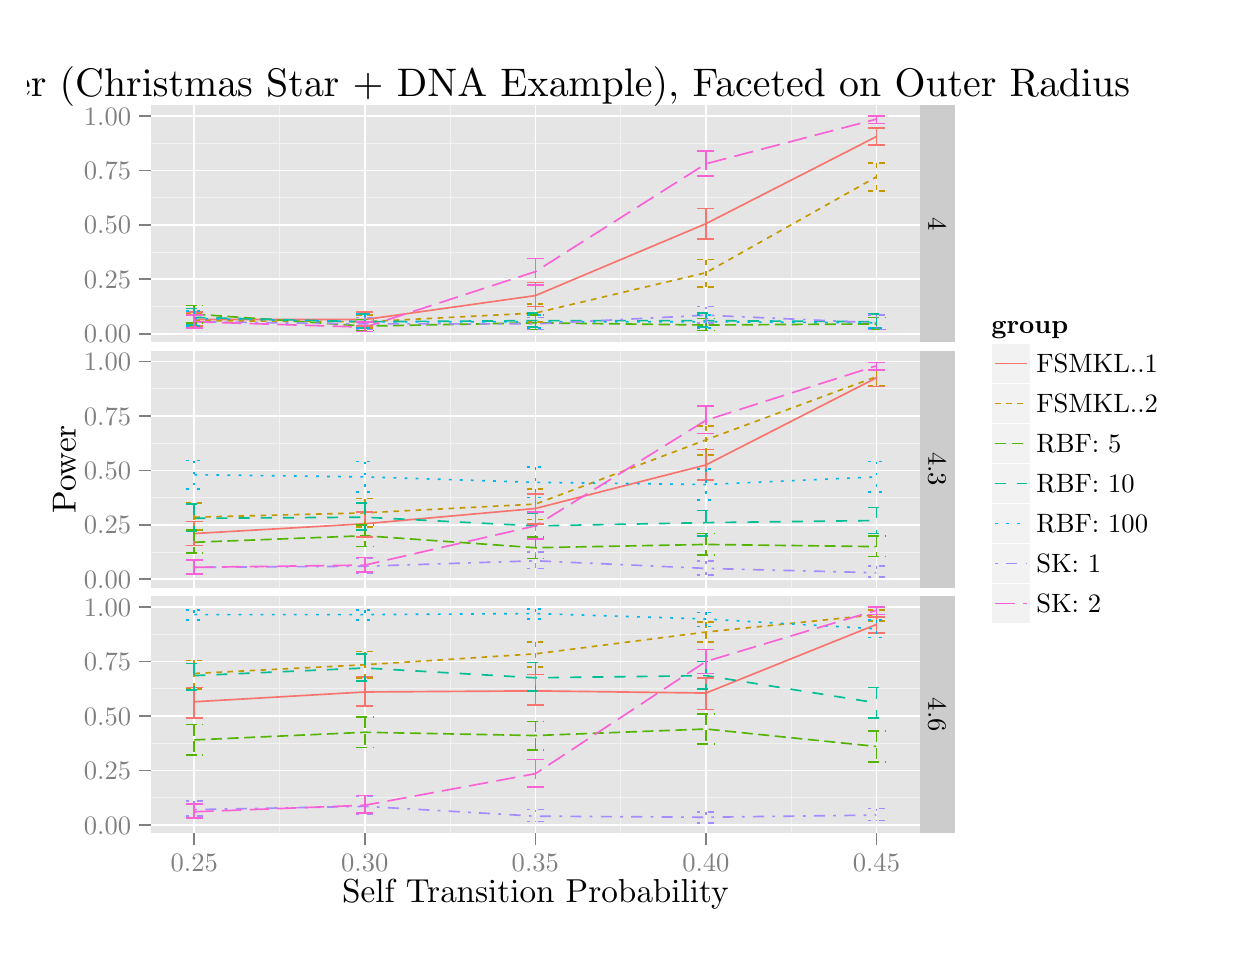
\begin{tikzpicture}[x=1pt,y=1pt]
\definecolor[named]{fillColor}{rgb}{1.00,1.00,1.00}
\path[use as bounding box,fill=fillColor,fill opacity=0.00] (0,0) rectangle (433.62,325.21);
\begin{scope}
\path[clip] (  0.00,  0.00) rectangle (433.62,325.21);
\definecolor[named]{drawColor}{rgb}{1.00,1.00,1.00}
\definecolor[named]{fillColor}{rgb}{1.00,1.00,1.00}

\path[draw=drawColor,line width= 0.6pt,line join=round,line cap=round,fill=fillColor] (  0.00,  0.00) rectangle (433.62,325.21);
\end{scope}
\begin{scope}
\path[clip] ( 44.49,211.51) rectangle (322.42,297.23);
\definecolor[named]{fillColor}{rgb}{0.90,0.90,0.90}

\path[fill=fillColor] ( 44.49,211.51) rectangle (322.42,297.23);
\definecolor[named]{drawColor}{rgb}{0.95,0.95,0.95}

\path[draw=drawColor,line width= 0.3pt,line join=round] ( 44.49,224.45) --
	(322.42,224.45);

\path[draw=drawColor,line width= 0.3pt,line join=round] ( 44.49,244.13) --
	(322.42,244.13);

\path[draw=drawColor,line width= 0.3pt,line join=round] ( 44.49,263.81) --
	(322.42,263.81);

\path[draw=drawColor,line width= 0.3pt,line join=round] ( 44.49,283.49) --
	(322.42,283.49);

\path[draw=drawColor,line width= 0.3pt,line join=round] ( 91.01,211.51) --
	( 91.01,297.23);

\path[draw=drawColor,line width= 0.3pt,line join=round] (152.64,211.51) --
	(152.64,297.23);

\path[draw=drawColor,line width= 0.3pt,line join=round] (214.27,211.51) --
	(214.27,297.23);

\path[draw=drawColor,line width= 0.3pt,line join=round] (275.89,211.51) --
	(275.89,297.23);
\definecolor[named]{drawColor}{rgb}{1.00,1.00,1.00}

\path[draw=drawColor,line width= 0.6pt,line join=round] ( 44.49,214.62) --
	(322.42,214.62);

\path[draw=drawColor,line width= 0.6pt,line join=round] ( 44.49,234.29) --
	(322.42,234.29);

\path[draw=drawColor,line width= 0.6pt,line join=round] ( 44.49,253.97) --
	(322.42,253.97);

\path[draw=drawColor,line width= 0.6pt,line join=round] ( 44.49,273.65) --
	(322.42,273.65);

\path[draw=drawColor,line width= 0.6pt,line join=round] ( 44.49,293.33) --
	(322.42,293.33);

\path[draw=drawColor,line width= 0.6pt,line join=round] ( 60.20,211.51) --
	( 60.20,297.23);

\path[draw=drawColor,line width= 0.6pt,line join=round] (121.83,211.51) --
	(121.83,297.23);

\path[draw=drawColor,line width= 0.6pt,line join=round] (183.45,211.51) --
	(183.45,297.23);

\path[draw=drawColor,line width= 0.6pt,line join=round] (245.08,211.51) --
	(245.08,297.23);

\path[draw=drawColor,line width= 0.6pt,line join=round] (306.70,211.51) --
	(306.70,297.23);
\definecolor[named]{drawColor}{rgb}{0.97,0.46,0.43}

\path[draw=drawColor,line width= 0.6pt,line join=round] ( 60.20,219.73) --
	(121.83,219.73) --
	(183.45,228.39) --
	(245.08,254.37) --
	(306.70,285.86);
\definecolor[named]{drawColor}{rgb}{0.77,0.60,0.00}

\path[draw=drawColor,line width= 0.6pt,dash pattern=on 2pt off 2pt ,line join=round] ( 60.20,219.34) --
	(121.83,218.94) --
	(183.45,222.09) --
	(245.08,236.66) --
	(306.70,271.29);
\definecolor[named]{drawColor}{rgb}{0.33,0.71,0.00}

\path[draw=drawColor,line width= 0.6pt,dash pattern=on 4pt off 2pt ,line join=round] ( 60.20,221.70) --
	(121.83,217.37) --
	(183.45,218.55) --
	(245.08,217.76) --
	(306.70,218.16);
\definecolor[named]{drawColor}{rgb}{0.00,0.75,0.58}

\path[draw=drawColor,line width= 0.6pt,dash pattern=on 4pt off 4pt ,line join=round] ( 60.20,220.52) --
	(121.83,218.94) --
	(183.45,219.34) --
	(245.08,219.34) --
	(306.70,218.94);
\definecolor[named]{drawColor}{rgb}{0.00,0.71,0.92}

\path[draw=drawColor,line width= 0.6pt,dash pattern=on 1pt off 3pt ,line join=round] ( 60.20,220.13) --
	(121.83,218.94) --
	(183.45,218.94) --
	(245.08,218.94) --
	(306.70,218.55);
\definecolor[named]{drawColor}{rgb}{0.65,0.54,1.00}

\path[draw=drawColor,line width= 0.6pt,dash pattern=on 1pt off 3pt on 4pt off 3pt ,line join=round] ( 60.20,218.94) --
	(121.83,218.16) --
	(183.45,218.16) --
	(245.08,221.31) --
	(306.70,218.55);
\definecolor[named]{drawColor}{rgb}{0.98,0.38,0.84}

\path[draw=drawColor,line width= 0.6pt,dash pattern=on 7pt off 3pt ,line join=round] ( 60.20,218.94) --
	(121.83,216.98) --
	(183.45,237.05) --
	(245.08,276.02) --
	(306.70,292.15);
\definecolor[named]{drawColor}{rgb}{0.97,0.46,0.43}

\path[draw=drawColor,line width= 0.6pt,line join=round] ( 57.12,222.49) --
	( 63.28,222.49);

\path[draw=drawColor,line width= 0.6pt,line join=round] ( 60.20,222.49) --
	( 60.20,217.36);

\path[draw=drawColor,line width= 0.6pt,line join=round] ( 57.12,217.36) --
	( 63.28,217.36);

\path[draw=drawColor,line width= 0.6pt,line join=round] (118.74,222.49) --
	(124.91,222.49);

\path[draw=drawColor,line width= 0.6pt,line join=round] (121.83,222.49) --
	(121.83,217.37);

\path[draw=drawColor,line width= 0.6pt,line join=round] (118.74,217.37) --
	(124.91,217.37);

\path[draw=drawColor,line width= 0.6pt,line join=round] (180.37,233.11) --
	(186.53,233.11);

\path[draw=drawColor,line width= 0.6pt,line join=round] (183.45,233.11) --
	(183.45,224.45);

\path[draw=drawColor,line width= 0.6pt,line join=round] (180.37,224.45) --
	(186.53,224.45);

\path[draw=drawColor,line width= 0.6pt,line join=round] (242.00,259.88) --
	(248.16,259.88);

\path[draw=drawColor,line width= 0.6pt,line join=round] (245.08,259.88) --
	(245.08,248.86);

\path[draw=drawColor,line width= 0.6pt,line join=round] (242.00,248.86) --
	(248.16,248.86);

\path[draw=drawColor,line width= 0.6pt,line join=round] (303.62,289.00) --
	(309.79,289.00);

\path[draw=drawColor,line width= 0.6pt,line join=round] (306.70,289.00) --
	(306.70,282.71);

\path[draw=drawColor,line width= 0.6pt,line join=round] (303.62,282.71) --
	(309.79,282.71);
\definecolor[named]{drawColor}{rgb}{0.77,0.60,0.00}

\path[draw=drawColor,line width= 0.6pt,dash pattern=on 2pt off 2pt ,line join=round] ( 57.12,221.70) --
	( 63.28,221.70);

\path[draw=drawColor,line width= 0.6pt,dash pattern=on 2pt off 2pt ,line join=round] ( 60.20,221.70) --
	( 60.20,216.98);

\path[draw=drawColor,line width= 0.6pt,dash pattern=on 2pt off 2pt ,line join=round] ( 57.12,216.98) --
	( 63.28,216.98);

\path[draw=drawColor,line width= 0.6pt,dash pattern=on 2pt off 2pt ,line join=round] (118.74,221.32) --
	(124.91,221.32);

\path[draw=drawColor,line width= 0.6pt,dash pattern=on 2pt off 2pt ,line join=round] (121.83,221.32) --
	(121.83,216.58);

\path[draw=drawColor,line width= 0.6pt,dash pattern=on 2pt off 2pt ,line join=round] (118.74,216.58) --
	(124.91,216.58);

\path[draw=drawColor,line width= 0.6pt,dash pattern=on 2pt off 2pt ,line join=round] (180.37,225.25) --
	(186.53,225.25);

\path[draw=drawColor,line width= 0.6pt,dash pattern=on 2pt off 2pt ,line join=round] (183.45,225.25) --
	(183.45,218.94);

\path[draw=drawColor,line width= 0.6pt,dash pattern=on 2pt off 2pt ,line join=round] (180.37,218.94) --
	(186.53,218.94);

\path[draw=drawColor,line width= 0.6pt,dash pattern=on 2pt off 2pt ,line join=round] (242.00,241.38) --
	(248.16,241.38);

\path[draw=drawColor,line width= 0.6pt,dash pattern=on 2pt off 2pt ,line join=round] (245.08,241.38) --
	(245.08,231.54);

\path[draw=drawColor,line width= 0.6pt,dash pattern=on 2pt off 2pt ,line join=round] (242.00,231.54) --
	(248.16,231.54);

\path[draw=drawColor,line width= 0.6pt,dash pattern=on 2pt off 2pt ,line join=round] (303.62,276.41) --
	(309.79,276.41);

\path[draw=drawColor,line width= 0.6pt,dash pattern=on 2pt off 2pt ,line join=round] (306.70,276.41) --
	(306.70,266.17);

\path[draw=drawColor,line width= 0.6pt,dash pattern=on 2pt off 2pt ,line join=round] (303.62,266.17) --
	(309.79,266.17);
\definecolor[named]{drawColor}{rgb}{0.33,0.71,0.00}

\path[draw=drawColor,line width= 0.6pt,dash pattern=on 4pt off 2pt ,line join=round] ( 57.12,224.85) --
	( 63.28,224.85);

\path[draw=drawColor,line width= 0.6pt,dash pattern=on 4pt off 2pt ,line join=round] ( 60.20,224.85) --
	( 60.20,218.55);

\path[draw=drawColor,line width= 0.6pt,dash pattern=on 4pt off 2pt ,line join=round] ( 57.12,218.55) --
	( 63.28,218.55);

\path[draw=drawColor,line width= 0.6pt,dash pattern=on 4pt off 2pt ,line join=round] (118.74,219.73) --
	(124.91,219.73);

\path[draw=drawColor,line width= 0.6pt,dash pattern=on 4pt off 2pt ,line join=round] (121.83,219.73) --
	(121.83,215.80);

\path[draw=drawColor,line width= 0.6pt,dash pattern=on 4pt off 2pt ,line join=round] (118.74,215.80) --
	(124.91,215.80);

\path[draw=drawColor,line width= 0.6pt,dash pattern=on 4pt off 2pt ,line join=round] (180.37,221.31) --
	(186.53,221.31);

\path[draw=drawColor,line width= 0.6pt,dash pattern=on 4pt off 2pt ,line join=round] (183.45,221.31) --
	(183.45,216.19);

\path[draw=drawColor,line width= 0.6pt,dash pattern=on 4pt off 2pt ,line join=round] (180.37,216.19) --
	(186.53,216.19);

\path[draw=drawColor,line width= 0.6pt,dash pattern=on 4pt off 2pt ,line join=round] (242.00,220.13) --
	(248.16,220.13);

\path[draw=drawColor,line width= 0.6pt,dash pattern=on 4pt off 2pt ,line join=round] (245.08,220.13) --
	(245.08,215.80);

\path[draw=drawColor,line width= 0.6pt,dash pattern=on 4pt off 2pt ,line join=round] (242.00,215.80) --
	(248.16,215.80);

\path[draw=drawColor,line width= 0.6pt,dash pattern=on 4pt off 2pt ,line join=round] (303.62,220.52) --
	(309.79,220.52);

\path[draw=drawColor,line width= 0.6pt,dash pattern=on 4pt off 2pt ,line join=round] (306.70,220.52) --
	(306.70,216.19);

\path[draw=drawColor,line width= 0.6pt,dash pattern=on 4pt off 2pt ,line join=round] (303.62,216.19) --
	(309.79,216.19);
\definecolor[named]{drawColor}{rgb}{0.00,0.75,0.58}

\path[draw=drawColor,line width= 0.6pt,dash pattern=on 4pt off 4pt ,line join=round] ( 57.12,223.67) --
	( 63.28,223.67);

\path[draw=drawColor,line width= 0.6pt,dash pattern=on 4pt off 4pt ,line join=round] ( 60.20,223.67) --
	( 60.20,217.76);

\path[draw=drawColor,line width= 0.6pt,dash pattern=on 4pt off 4pt ,line join=round] ( 57.12,217.76) --
	( 63.28,217.76);

\path[draw=drawColor,line width= 0.6pt,dash pattern=on 4pt off 4pt ,line join=round] (118.74,221.70) --
	(124.91,221.70);

\path[draw=drawColor,line width= 0.6pt,dash pattern=on 4pt off 4pt ,line join=round] (121.83,221.70) --
	(121.83,216.58);

\path[draw=drawColor,line width= 0.6pt,dash pattern=on 4pt off 4pt ,line join=round] (118.74,216.58) --
	(124.91,216.58);

\path[draw=drawColor,line width= 0.6pt,dash pattern=on 4pt off 4pt ,line join=round] (180.37,222.09) --
	(186.53,222.09);

\path[draw=drawColor,line width= 0.6pt,dash pattern=on 4pt off 4pt ,line join=round] (183.45,222.09) --
	(183.45,216.98);

\path[draw=drawColor,line width= 0.6pt,dash pattern=on 4pt off 4pt ,line join=round] (180.37,216.98) --
	(186.53,216.98);

\path[draw=drawColor,line width= 0.6pt,dash pattern=on 4pt off 4pt ,line join=round] (242.00,222.09) --
	(248.16,222.09);

\path[draw=drawColor,line width= 0.6pt,dash pattern=on 4pt off 4pt ,line join=round] (245.08,222.09) --
	(245.08,216.98);

\path[draw=drawColor,line width= 0.6pt,dash pattern=on 4pt off 4pt ,line join=round] (242.00,216.98) --
	(248.16,216.98);

\path[draw=drawColor,line width= 0.6pt,dash pattern=on 4pt off 4pt ,line join=round] (303.62,221.70) --
	(309.79,221.70);

\path[draw=drawColor,line width= 0.6pt,dash pattern=on 4pt off 4pt ,line join=round] (306.70,221.70) --
	(306.70,216.58);

\path[draw=drawColor,line width= 0.6pt,dash pattern=on 4pt off 4pt ,line join=round] (303.62,216.58) --
	(309.79,216.58);
\definecolor[named]{drawColor}{rgb}{0.00,0.71,0.92}

\path[draw=drawColor,line width= 0.6pt,dash pattern=on 1pt off 3pt ,line join=round] ( 57.12,222.88) --
	( 63.28,222.88);

\path[draw=drawColor,line width= 0.6pt,dash pattern=on 1pt off 3pt ,line join=round] ( 60.20,222.88) --
	( 60.20,217.37);

\path[draw=drawColor,line width= 0.6pt,dash pattern=on 1pt off 3pt ,line join=round] ( 57.12,217.37) --
	( 63.28,217.37);

\path[draw=drawColor,line width= 0.6pt,dash pattern=on 1pt off 3pt ,line join=round] (118.74,221.70) --
	(124.91,221.70);

\path[draw=drawColor,line width= 0.6pt,dash pattern=on 1pt off 3pt ,line join=round] (121.83,221.70) --
	(121.83,216.58);

\path[draw=drawColor,line width= 0.6pt,dash pattern=on 1pt off 3pt ,line join=round] (118.74,216.58) --
	(124.91,216.58);

\path[draw=drawColor,line width= 0.6pt,dash pattern=on 1pt off 3pt ,line join=round] (180.37,221.31) --
	(186.53,221.31);

\path[draw=drawColor,line width= 0.6pt,dash pattern=on 1pt off 3pt ,line join=round] (183.45,221.31) --
	(183.45,216.58);

\path[draw=drawColor,line width= 0.6pt,dash pattern=on 1pt off 3pt ,line join=round] (180.37,216.58) --
	(186.53,216.58);

\path[draw=drawColor,line width= 0.6pt,dash pattern=on 1pt off 3pt ,line join=round] (242.00,221.32) --
	(248.16,221.32);

\path[draw=drawColor,line width= 0.6pt,dash pattern=on 1pt off 3pt ,line join=round] (245.08,221.32) --
	(245.08,216.58);

\path[draw=drawColor,line width= 0.6pt,dash pattern=on 1pt off 3pt ,line join=round] (242.00,216.58) --
	(248.16,216.58);

\path[draw=drawColor,line width= 0.6pt,dash pattern=on 1pt off 3pt ,line join=round] (303.62,221.31) --
	(309.79,221.31);

\path[draw=drawColor,line width= 0.6pt,dash pattern=on 1pt off 3pt ,line join=round] (306.70,221.31) --
	(306.70,216.57);

\path[draw=drawColor,line width= 0.6pt,dash pattern=on 1pt off 3pt ,line join=round] (303.62,216.57) --
	(309.79,216.57);
\definecolor[named]{drawColor}{rgb}{0.65,0.54,1.00}

\path[draw=drawColor,line width= 0.6pt,dash pattern=on 1pt off 3pt on 4pt off 3pt ,line join=round] ( 57.12,221.32) --
	( 63.28,221.32);

\path[draw=drawColor,line width= 0.6pt,dash pattern=on 1pt off 3pt on 4pt off 3pt ,line join=round] ( 60.20,221.32) --
	( 60.20,216.58);

\path[draw=drawColor,line width= 0.6pt,dash pattern=on 1pt off 3pt on 4pt off 3pt ,line join=round] ( 57.12,216.58) --
	( 63.28,216.58);

\path[draw=drawColor,line width= 0.6pt,dash pattern=on 1pt off 3pt on 4pt off 3pt ,line join=round] (118.74,220.52) --
	(124.91,220.52);

\path[draw=drawColor,line width= 0.6pt,dash pattern=on 1pt off 3pt on 4pt off 3pt ,line join=round] (121.83,220.52) --
	(121.83,216.19);

\path[draw=drawColor,line width= 0.6pt,dash pattern=on 1pt off 3pt on 4pt off 3pt ,line join=round] (118.74,216.19) --
	(124.91,216.19);

\path[draw=drawColor,line width= 0.6pt,dash pattern=on 1pt off 3pt on 4pt off 3pt ,line join=round] (180.37,220.52) --
	(186.53,220.52);

\path[draw=drawColor,line width= 0.6pt,dash pattern=on 1pt off 3pt on 4pt off 3pt ,line join=round] (183.45,220.52) --
	(183.45,216.19);

\path[draw=drawColor,line width= 0.6pt,dash pattern=on 1pt off 3pt on 4pt off 3pt ,line join=round] (180.37,216.19) --
	(186.53,216.19);

\path[draw=drawColor,line width= 0.6pt,dash pattern=on 1pt off 3pt on 4pt off 3pt ,line join=round] (242.00,224.45) --
	(248.16,224.45);

\path[draw=drawColor,line width= 0.6pt,dash pattern=on 1pt off 3pt on 4pt off 3pt ,line join=round] (245.08,224.45) --
	(245.08,218.55);

\path[draw=drawColor,line width= 0.6pt,dash pattern=on 1pt off 3pt on 4pt off 3pt ,line join=round] (242.00,218.55) --
	(248.16,218.55);

\path[draw=drawColor,line width= 0.6pt,dash pattern=on 1pt off 3pt on 4pt off 3pt ,line join=round] (303.62,221.31) --
	(309.79,221.31);

\path[draw=drawColor,line width= 0.6pt,dash pattern=on 1pt off 3pt on 4pt off 3pt ,line join=round] (306.70,221.31) --
	(306.70,216.19);

\path[draw=drawColor,line width= 0.6pt,dash pattern=on 1pt off 3pt on 4pt off 3pt ,line join=round] (303.62,216.19) --
	(309.79,216.19);
\definecolor[named]{drawColor}{rgb}{0.98,0.38,0.84}

\path[draw=drawColor,line width= 0.6pt,dash pattern=on 7pt off 3pt ,line join=round] ( 57.12,221.31) --
	( 63.28,221.31);

\path[draw=drawColor,line width= 0.6pt,dash pattern=on 7pt off 3pt ,line join=round] ( 60.20,221.31) --
	( 60.20,216.58);

\path[draw=drawColor,line width= 0.6pt,dash pattern=on 7pt off 3pt ,line join=round] ( 57.12,216.58) --
	( 63.28,216.58);

\path[draw=drawColor,line width= 0.6pt,dash pattern=on 7pt off 3pt ,line join=round] (118.74,218.94) --
	(124.91,218.94);

\path[draw=drawColor,line width= 0.6pt,dash pattern=on 7pt off 3pt ,line join=round] (121.83,218.94) --
	(121.83,215.40);

\path[draw=drawColor,line width= 0.6pt,dash pattern=on 7pt off 3pt ,line join=round] (118.74,215.40) --
	(124.91,215.40);

\path[draw=drawColor,line width= 0.6pt,dash pattern=on 7pt off 3pt ,line join=round] (180.37,241.77) --
	(186.53,241.77);

\path[draw=drawColor,line width= 0.6pt,dash pattern=on 7pt off 3pt ,line join=round] (183.45,241.77) --
	(183.45,232.33);

\path[draw=drawColor,line width= 0.6pt,dash pattern=on 7pt off 3pt ,line join=round] (180.37,232.33) --
	(186.53,232.33);

\path[draw=drawColor,line width= 0.6pt,dash pattern=on 7pt off 3pt ,line join=round] (242.00,280.74) --
	(248.16,280.74);

\path[draw=drawColor,line width= 0.6pt,dash pattern=on 7pt off 3pt ,line join=round] (245.08,280.74) --
	(245.08,271.69);

\path[draw=drawColor,line width= 0.6pt,dash pattern=on 7pt off 3pt ,line join=round] (242.00,271.69) --
	(248.16,271.69);

\path[draw=drawColor,line width= 0.6pt,dash pattern=on 7pt off 3pt ,line join=round] (303.62,293.33) --
	(309.79,293.33);

\path[draw=drawColor,line width= 0.6pt,dash pattern=on 7pt off 3pt ,line join=round] (306.70,293.33) --
	(306.70,290.58);

\path[draw=drawColor,line width= 0.6pt,dash pattern=on 7pt off 3pt ,line join=round] (303.62,290.58) --
	(309.79,290.58);
\end{scope}
\begin{scope}
\path[clip] ( 44.49,122.77) rectangle (322.42,208.49);
\definecolor[named]{fillColor}{rgb}{0.90,0.90,0.90}

\path[fill=fillColor] ( 44.49,122.77) rectangle (322.42,208.49);
\definecolor[named]{drawColor}{rgb}{0.95,0.95,0.95}

\path[draw=drawColor,line width= 0.3pt,line join=round] ( 44.49,135.72) --
	(322.42,135.72);

\path[draw=drawColor,line width= 0.3pt,line join=round] ( 44.49,155.40) --
	(322.42,155.40);

\path[draw=drawColor,line width= 0.3pt,line join=round] ( 44.49,175.08) --
	(322.42,175.08);

\path[draw=drawColor,line width= 0.3pt,line join=round] ( 44.49,194.76) --
	(322.42,194.76);

\path[draw=drawColor,line width= 0.3pt,line join=round] ( 91.01,122.77) --
	( 91.01,208.49);

\path[draw=drawColor,line width= 0.3pt,line join=round] (152.64,122.77) --
	(152.64,208.49);

\path[draw=drawColor,line width= 0.3pt,line join=round] (214.27,122.77) --
	(214.27,208.49);

\path[draw=drawColor,line width= 0.3pt,line join=round] (275.89,122.77) --
	(275.89,208.49);
\definecolor[named]{drawColor}{rgb}{1.00,1.00,1.00}

\path[draw=drawColor,line width= 0.6pt,line join=round] ( 44.49,125.88) --
	(322.42,125.88);

\path[draw=drawColor,line width= 0.6pt,line join=round] ( 44.49,145.56) --
	(322.42,145.56);

\path[draw=drawColor,line width= 0.6pt,line join=round] ( 44.49,165.24) --
	(322.42,165.24);

\path[draw=drawColor,line width= 0.6pt,line join=round] ( 44.49,184.92) --
	(322.42,184.92);

\path[draw=drawColor,line width= 0.6pt,line join=round] ( 44.49,204.60) --
	(322.42,204.60);

\path[draw=drawColor,line width= 0.6pt,line join=round] ( 60.20,122.77) --
	( 60.20,208.49);

\path[draw=drawColor,line width= 0.6pt,line join=round] (121.83,122.77) --
	(121.83,208.49);

\path[draw=drawColor,line width= 0.6pt,line join=round] (183.45,122.77) --
	(183.45,208.49);

\path[draw=drawColor,line width= 0.6pt,line join=round] (245.08,122.77) --
	(245.08,208.49);

\path[draw=drawColor,line width= 0.6pt,line join=round] (306.70,122.77) --
	(306.70,208.49);
\definecolor[named]{drawColor}{rgb}{0.97,0.46,0.43}

\path[draw=drawColor,line width= 0.6pt,line join=round] ( 60.20,142.41) --
	(121.83,145.95) --
	(183.45,151.46) --
	(245.08,167.21) --
	(306.70,198.69);
\definecolor[named]{drawColor}{rgb}{0.77,0.60,0.00}

\path[draw=drawColor,line width= 0.6pt,dash pattern=on 2pt off 2pt ,line join=round] ( 60.20,148.31) --
	(121.83,149.89) --
	(183.45,153.04) --
	(245.08,176.26) --
	(306.70,199.09);
\definecolor[named]{drawColor}{rgb}{0.33,0.71,0.00}

\path[draw=drawColor,line width= 0.6pt,dash pattern=on 4pt off 2pt ,line join=round] ( 60.20,139.26) --
	(121.83,141.62) --
	(183.45,137.29) --
	(245.08,138.47) --
	(306.70,137.69);
\definecolor[named]{drawColor}{rgb}{0.00,0.75,0.58}

\path[draw=drawColor,line width= 0.6pt,dash pattern=on 4pt off 4pt ,line join=round] ( 60.20,147.92) --
	(121.83,148.31) --
	(183.45,145.17) --
	(245.08,146.35) --
	(306.70,147.13);
\definecolor[named]{drawColor}{rgb}{0.00,0.71,0.92}

\path[draw=drawColor,line width= 0.6pt,dash pattern=on 1pt off 3pt ,line join=round] ( 60.20,163.66) --
	(121.83,162.88) --
	(183.45,160.91) --
	(245.08,160.12) --
	(306.70,162.88);
\definecolor[named]{drawColor}{rgb}{0.65,0.54,1.00}

\path[draw=drawColor,line width= 0.6pt,dash pattern=on 1pt off 3pt on 4pt off 3pt ,line join=round] ( 60.20,130.21) --
	(121.83,130.60) --
	(183.45,132.57) --
	(245.08,129.82) --
	(306.70,128.24);
\definecolor[named]{drawColor}{rgb}{0.98,0.38,0.84}

\path[draw=drawColor,line width= 0.6pt,dash pattern=on 7pt off 3pt ,line join=round] ( 60.20,130.21) --
	(121.83,131.00) --
	(183.45,145.17) --
	(245.08,183.34) --
	(306.70,203.02);
\definecolor[named]{drawColor}{rgb}{0.97,0.46,0.43}

\path[draw=drawColor,line width= 0.6pt,line join=round] ( 57.12,146.74) --
	( 63.28,146.74);

\path[draw=drawColor,line width= 0.6pt,line join=round] ( 60.20,146.74) --
	( 60.20,138.08);

\path[draw=drawColor,line width= 0.6pt,line join=round] ( 57.12,138.08) --
	( 63.28,138.08);

\path[draw=drawColor,line width= 0.6pt,line join=round] (118.74,150.28) --
	(124.91,150.28);

\path[draw=drawColor,line width= 0.6pt,line join=round] (121.83,150.28) --
	(121.83,141.23);

\path[draw=drawColor,line width= 0.6pt,line join=round] (118.74,141.23) --
	(124.91,141.23);

\path[draw=drawColor,line width= 0.6pt,line join=round] (180.37,156.59) --
	(186.53,156.59);

\path[draw=drawColor,line width= 0.6pt,line join=round] (183.45,156.59) --
	(183.45,145.95);

\path[draw=drawColor,line width= 0.6pt,line join=round] (180.37,145.95) --
	(186.53,145.95);

\path[draw=drawColor,line width= 0.6pt,line join=round] (242.00,172.73) --
	(248.16,172.73);

\path[draw=drawColor,line width= 0.6pt,line join=round] (245.08,172.73) --
	(245.08,161.69);

\path[draw=drawColor,line width= 0.6pt,line join=round] (242.00,161.69) --
	(248.16,161.69);

\path[draw=drawColor,line width= 0.6pt,line join=round] (303.62,201.45) --
	(309.79,201.45);

\path[draw=drawColor,line width= 0.6pt,line join=round] (306.70,201.45) --
	(306.70,195.55);

\path[draw=drawColor,line width= 0.6pt,line join=round] (303.62,195.55) --
	(309.79,195.55);
\definecolor[named]{drawColor}{rgb}{0.77,0.60,0.00}

\path[draw=drawColor,line width= 0.6pt,dash pattern=on 2pt off 2pt ,line join=round] ( 57.12,153.43) --
	( 63.28,153.43);

\path[draw=drawColor,line width= 0.6pt,dash pattern=on 2pt off 2pt ,line join=round] ( 60.20,153.43) --
	( 60.20,143.59);

\path[draw=drawColor,line width= 0.6pt,dash pattern=on 2pt off 2pt ,line join=round] ( 57.12,143.59) --
	( 63.28,143.59);

\path[draw=drawColor,line width= 0.6pt,dash pattern=on 2pt off 2pt ,line join=round] (118.74,155.02) --
	(124.91,155.02);

\path[draw=drawColor,line width= 0.6pt,dash pattern=on 2pt off 2pt ,line join=round] (121.83,155.02) --
	(121.83,144.77);

\path[draw=drawColor,line width= 0.6pt,dash pattern=on 2pt off 2pt ,line join=round] (118.74,144.77) --
	(124.91,144.77);

\path[draw=drawColor,line width= 0.6pt,dash pattern=on 2pt off 2pt ,line join=round] (180.37,158.55) --
	(186.53,158.55);

\path[draw=drawColor,line width= 0.6pt,dash pattern=on 2pt off 2pt ,line join=round] (183.45,158.55) --
	(183.45,147.53);

\path[draw=drawColor,line width= 0.6pt,dash pattern=on 2pt off 2pt ,line join=round] (180.37,147.53) --
	(186.53,147.53);

\path[draw=drawColor,line width= 0.6pt,dash pattern=on 2pt off 2pt ,line join=round] (242.00,181.38) --
	(248.16,181.38);

\path[draw=drawColor,line width= 0.6pt,dash pattern=on 2pt off 2pt ,line join=round] (245.08,181.38) --
	(245.08,170.75);

\path[draw=drawColor,line width= 0.6pt,dash pattern=on 2pt off 2pt ,line join=round] (242.00,170.75) --
	(248.16,170.75);

\path[draw=drawColor,line width= 0.6pt,dash pattern=on 2pt off 2pt ,line join=round] (303.62,201.45) --
	(309.79,201.45);

\path[draw=drawColor,line width= 0.6pt,dash pattern=on 2pt off 2pt ,line join=round] (306.70,201.45) --
	(306.70,195.94);

\path[draw=drawColor,line width= 0.6pt,dash pattern=on 2pt off 2pt ,line join=round] (303.62,195.94) --
	(309.79,195.94);
\definecolor[named]{drawColor}{rgb}{0.33,0.71,0.00}

\path[draw=drawColor,line width= 0.6pt,dash pattern=on 4pt off 2pt ,line join=round] ( 57.12,143.59) --
	( 63.28,143.59);

\path[draw=drawColor,line width= 0.6pt,dash pattern=on 4pt off 2pt ,line join=round] ( 60.20,143.59) --
	( 60.20,135.33);

\path[draw=drawColor,line width= 0.6pt,dash pattern=on 4pt off 2pt ,line join=round] ( 57.12,135.33) --
	( 63.28,135.33);

\path[draw=drawColor,line width= 0.6pt,dash pattern=on 4pt off 2pt ,line join=round] (118.74,145.57) --
	(124.91,145.57);

\path[draw=drawColor,line width= 0.6pt,dash pattern=on 4pt off 2pt ,line join=round] (121.83,145.57) --
	(121.83,137.69);

\path[draw=drawColor,line width= 0.6pt,dash pattern=on 4pt off 2pt ,line join=round] (118.74,137.69) --
	(124.91,137.69);

\path[draw=drawColor,line width= 0.6pt,dash pattern=on 4pt off 2pt ,line join=round] (180.37,141.23) --
	(186.53,141.23);

\path[draw=drawColor,line width= 0.6pt,dash pattern=on 4pt off 2pt ,line join=round] (183.45,141.23) --
	(183.45,133.36);

\path[draw=drawColor,line width= 0.6pt,dash pattern=on 4pt off 2pt ,line join=round] (180.37,133.36) --
	(186.53,133.36);

\path[draw=drawColor,line width= 0.6pt,dash pattern=on 4pt off 2pt ,line join=round] (242.00,142.42) --
	(248.16,142.42);

\path[draw=drawColor,line width= 0.6pt,dash pattern=on 4pt off 2pt ,line join=round] (245.08,142.42) --
	(245.08,134.54);

\path[draw=drawColor,line width= 0.6pt,dash pattern=on 4pt off 2pt ,line join=round] (242.00,134.54) --
	(248.16,134.54);

\path[draw=drawColor,line width= 0.6pt,dash pattern=on 4pt off 2pt ,line join=round] (303.62,141.62) --
	(309.79,141.62);

\path[draw=drawColor,line width= 0.6pt,dash pattern=on 4pt off 2pt ,line join=round] (306.70,141.62) --
	(306.70,134.14);

\path[draw=drawColor,line width= 0.6pt,dash pattern=on 4pt off 2pt ,line join=round] (303.62,134.14) --
	(309.79,134.14);
\definecolor[named]{drawColor}{rgb}{0.00,0.75,0.58}

\path[draw=drawColor,line width= 0.6pt,dash pattern=on 4pt off 4pt ,line join=round] ( 57.12,153.04) --
	( 63.28,153.04);

\path[draw=drawColor,line width= 0.6pt,dash pattern=on 4pt off 4pt ,line join=round] ( 60.20,153.04) --
	( 60.20,143.20);

\path[draw=drawColor,line width= 0.6pt,dash pattern=on 4pt off 4pt ,line join=round] ( 57.12,143.20) --
	( 63.28,143.20);

\path[draw=drawColor,line width= 0.6pt,dash pattern=on 4pt off 4pt ,line join=round] (118.74,153.43) --
	(124.91,153.43);

\path[draw=drawColor,line width= 0.6pt,dash pattern=on 4pt off 4pt ,line join=round] (121.83,153.43) --
	(121.83,143.59);

\path[draw=drawColor,line width= 0.6pt,dash pattern=on 4pt off 4pt ,line join=round] (118.74,143.59) --
	(124.91,143.59);

\path[draw=drawColor,line width= 0.6pt,dash pattern=on 4pt off 4pt ,line join=round] (180.37,149.89) --
	(186.53,149.89);

\path[draw=drawColor,line width= 0.6pt,dash pattern=on 4pt off 4pt ,line join=round] (183.45,149.89) --
	(183.45,140.44);

\path[draw=drawColor,line width= 0.6pt,dash pattern=on 4pt off 4pt ,line join=round] (180.37,140.44) --
	(186.53,140.44);

\path[draw=drawColor,line width= 0.6pt,dash pattern=on 4pt off 4pt ,line join=round] (242.00,150.68) --
	(248.16,150.68);

\path[draw=drawColor,line width= 0.6pt,dash pattern=on 4pt off 4pt ,line join=round] (245.08,150.68) --
	(245.08,141.62);

\path[draw=drawColor,line width= 0.6pt,dash pattern=on 4pt off 4pt ,line join=round] (242.00,141.62) --
	(248.16,141.62);

\path[draw=drawColor,line width= 0.6pt,dash pattern=on 4pt off 4pt ,line join=round] (303.62,151.86) --
	(309.79,151.86);

\path[draw=drawColor,line width= 0.6pt,dash pattern=on 4pt off 4pt ,line join=round] (306.70,151.86) --
	(306.70,142.40);

\path[draw=drawColor,line width= 0.6pt,dash pattern=on 4pt off 4pt ,line join=round] (303.62,142.40) --
	(309.79,142.40);
\definecolor[named]{drawColor}{rgb}{0.00,0.71,0.92}

\path[draw=drawColor,line width= 0.6pt,dash pattern=on 1pt off 3pt ,line join=round] ( 57.12,168.78) --
	( 63.28,168.78);

\path[draw=drawColor,line width= 0.6pt,dash pattern=on 1pt off 3pt ,line join=round] ( 60.20,168.78) --
	( 60.20,158.54);

\path[draw=drawColor,line width= 0.6pt,dash pattern=on 1pt off 3pt ,line join=round] ( 57.12,158.54) --
	( 63.28,158.54);

\path[draw=drawColor,line width= 0.6pt,dash pattern=on 1pt off 3pt ,line join=round] (118.74,168.39) --
	(124.91,168.39);

\path[draw=drawColor,line width= 0.6pt,dash pattern=on 1pt off 3pt ,line join=round] (121.83,168.39) --
	(121.83,157.37);

\path[draw=drawColor,line width= 0.6pt,dash pattern=on 1pt off 3pt ,line join=round] (118.74,157.37) --
	(124.91,157.37);

\path[draw=drawColor,line width= 0.6pt,dash pattern=on 1pt off 3pt ,line join=round] (180.37,166.42) --
	(186.53,166.42);

\path[draw=drawColor,line width= 0.6pt,dash pattern=on 1pt off 3pt ,line join=round] (183.45,166.42) --
	(183.45,155.40);

\path[draw=drawColor,line width= 0.6pt,dash pattern=on 1pt off 3pt ,line join=round] (180.37,155.40) --
	(186.53,155.40);

\path[draw=drawColor,line width= 0.6pt,dash pattern=on 1pt off 3pt ,line join=round] (242.00,165.63) --
	(248.16,165.63);

\path[draw=drawColor,line width= 0.6pt,dash pattern=on 1pt off 3pt ,line join=round] (245.08,165.63) --
	(245.08,154.61);

\path[draw=drawColor,line width= 0.6pt,dash pattern=on 1pt off 3pt ,line join=round] (242.00,154.61) --
	(248.16,154.61);

\path[draw=drawColor,line width= 0.6pt,dash pattern=on 1pt off 3pt ,line join=round] (303.62,168.39) --
	(309.79,168.39);

\path[draw=drawColor,line width= 0.6pt,dash pattern=on 1pt off 3pt ,line join=round] (306.70,168.39) --
	(306.70,157.37);

\path[draw=drawColor,line width= 0.6pt,dash pattern=on 1pt off 3pt ,line join=round] (303.62,157.37) --
	(309.79,157.37);
\definecolor[named]{drawColor}{rgb}{0.65,0.54,1.00}

\path[draw=drawColor,line width= 0.6pt,dash pattern=on 1pt off 3pt on 4pt off 3pt ,line join=round] ( 57.12,132.96) --
	( 63.28,132.96);

\path[draw=drawColor,line width= 0.6pt,dash pattern=on 1pt off 3pt on 4pt off 3pt ,line join=round] ( 60.20,132.96) --
	( 60.20,127.85);

\path[draw=drawColor,line width= 0.6pt,dash pattern=on 1pt off 3pt on 4pt off 3pt ,line join=round] ( 57.12,127.85) --
	( 63.28,127.85);

\path[draw=drawColor,line width= 0.6pt,dash pattern=on 1pt off 3pt on 4pt off 3pt ,line join=round] (118.74,133.36) --
	(124.91,133.36);

\path[draw=drawColor,line width= 0.6pt,dash pattern=on 1pt off 3pt on 4pt off 3pt ,line join=round] (121.83,133.36) --
	(121.83,128.24);

\path[draw=drawColor,line width= 0.6pt,dash pattern=on 1pt off 3pt on 4pt off 3pt ,line join=round] (118.74,128.24) --
	(124.91,128.24);

\path[draw=drawColor,line width= 0.6pt,dash pattern=on 1pt off 3pt on 4pt off 3pt ,line join=round] (180.37,135.72) --
	(186.53,135.72);

\path[draw=drawColor,line width= 0.6pt,dash pattern=on 1pt off 3pt on 4pt off 3pt ,line join=round] (183.45,135.72) --
	(183.45,129.82);

\path[draw=drawColor,line width= 0.6pt,dash pattern=on 1pt off 3pt on 4pt off 3pt ,line join=round] (180.37,129.82) --
	(186.53,129.82);

\path[draw=drawColor,line width= 0.6pt,dash pattern=on 1pt off 3pt on 4pt off 3pt ,line join=round] (242.00,132.57) --
	(248.16,132.57);

\path[draw=drawColor,line width= 0.6pt,dash pattern=on 1pt off 3pt on 4pt off 3pt ,line join=round] (245.08,132.57) --
	(245.08,127.45);

\path[draw=drawColor,line width= 0.6pt,dash pattern=on 1pt off 3pt on 4pt off 3pt ,line join=round] (242.00,127.45) --
	(248.16,127.45);

\path[draw=drawColor,line width= 0.6pt,dash pattern=on 1pt off 3pt on 4pt off 3pt ,line join=round] (303.62,130.60) --
	(309.79,130.60);

\path[draw=drawColor,line width= 0.6pt,dash pattern=on 1pt off 3pt on 4pt off 3pt ,line join=round] (306.70,130.60) --
	(306.70,126.67);

\path[draw=drawColor,line width= 0.6pt,dash pattern=on 1pt off 3pt on 4pt off 3pt ,line join=round] (303.62,126.67) --
	(309.79,126.67);
\definecolor[named]{drawColor}{rgb}{0.98,0.38,0.84}

\path[draw=drawColor,line width= 0.6pt,dash pattern=on 7pt off 3pt ,line join=round] ( 57.12,132.96) --
	( 63.28,132.96);

\path[draw=drawColor,line width= 0.6pt,dash pattern=on 7pt off 3pt ,line join=round] ( 60.20,132.96) --
	( 60.20,127.85);

\path[draw=drawColor,line width= 0.6pt,dash pattern=on 7pt off 3pt ,line join=round] ( 57.12,127.85) --
	( 63.28,127.85);

\path[draw=drawColor,line width= 0.6pt,dash pattern=on 7pt off 3pt ,line join=round] (118.74,133.75) --
	(124.91,133.75);

\path[draw=drawColor,line width= 0.6pt,dash pattern=on 7pt off 3pt ,line join=round] (121.83,133.75) --
	(121.83,128.62);

\path[draw=drawColor,line width= 0.6pt,dash pattern=on 7pt off 3pt ,line join=round] (118.74,128.62) --
	(124.91,128.62);

\path[draw=drawColor,line width= 0.6pt,dash pattern=on 7pt off 3pt ,line join=round] (180.37,150.28) --
	(186.53,150.28);

\path[draw=drawColor,line width= 0.6pt,dash pattern=on 7pt off 3pt ,line join=round] (183.45,150.28) --
	(183.45,140.44);

\path[draw=drawColor,line width= 0.6pt,dash pattern=on 7pt off 3pt ,line join=round] (180.37,140.44) --
	(186.53,140.44);

\path[draw=drawColor,line width= 0.6pt,dash pattern=on 7pt off 3pt ,line join=round] (242.00,188.46) --
	(248.16,188.46);

\path[draw=drawColor,line width= 0.6pt,dash pattern=on 7pt off 3pt ,line join=round] (245.08,188.46) --
	(245.08,178.62);

\path[draw=drawColor,line width= 0.6pt,dash pattern=on 7pt off 3pt ,line join=round] (242.00,178.62) --
	(248.16,178.62);

\path[draw=drawColor,line width= 0.6pt,dash pattern=on 7pt off 3pt ,line join=round] (303.62,204.20) --
	(309.79,204.20);

\path[draw=drawColor,line width= 0.6pt,dash pattern=on 7pt off 3pt ,line join=round] (306.70,204.20) --
	(306.70,201.45);

\path[draw=drawColor,line width= 0.6pt,dash pattern=on 7pt off 3pt ,line join=round] (303.62,201.45) --
	(309.79,201.45);
\end{scope}
\begin{scope}
\path[clip] ( 44.49, 34.03) rectangle (322.42,119.76);
\definecolor[named]{fillColor}{rgb}{0.90,0.90,0.90}

\path[fill=fillColor] ( 44.49, 34.03) rectangle (322.42,119.76);
\definecolor[named]{drawColor}{rgb}{0.95,0.95,0.95}

\path[draw=drawColor,line width= 0.3pt,line join=round] ( 44.49, 46.98) --
	(322.42, 46.98);

\path[draw=drawColor,line width= 0.3pt,line join=round] ( 44.49, 66.66) --
	(322.42, 66.66);

\path[draw=drawColor,line width= 0.3pt,line join=round] ( 44.49, 86.34) --
	(322.42, 86.34);

\path[draw=drawColor,line width= 0.3pt,line join=round] ( 44.49,106.02) --
	(322.42,106.02);

\path[draw=drawColor,line width= 0.3pt,line join=round] ( 91.01, 34.03) --
	( 91.01,119.76);

\path[draw=drawColor,line width= 0.3pt,line join=round] (152.64, 34.03) --
	(152.64,119.76);

\path[draw=drawColor,line width= 0.3pt,line join=round] (214.27, 34.03) --
	(214.27,119.76);

\path[draw=drawColor,line width= 0.3pt,line join=round] (275.89, 34.03) --
	(275.89,119.76);
\definecolor[named]{drawColor}{rgb}{1.00,1.00,1.00}

\path[draw=drawColor,line width= 0.6pt,line join=round] ( 44.49, 37.14) --
	(322.42, 37.14);

\path[draw=drawColor,line width= 0.6pt,line join=round] ( 44.49, 56.82) --
	(322.42, 56.82);

\path[draw=drawColor,line width= 0.6pt,line join=round] ( 44.49, 76.50) --
	(322.42, 76.50);

\path[draw=drawColor,line width= 0.6pt,line join=round] ( 44.49, 96.18) --
	(322.42, 96.18);

\path[draw=drawColor,line width= 0.6pt,line join=round] ( 44.49,115.86) --
	(322.42,115.86);

\path[draw=drawColor,line width= 0.6pt,line join=round] ( 60.20, 34.03) --
	( 60.20,119.76);

\path[draw=drawColor,line width= 0.6pt,line join=round] (121.83, 34.03) --
	(121.83,119.76);

\path[draw=drawColor,line width= 0.6pt,line join=round] (183.45, 34.03) --
	(183.45,119.76);

\path[draw=drawColor,line width= 0.6pt,line join=round] (245.08, 34.03) --
	(245.08,119.76);

\path[draw=drawColor,line width= 0.6pt,line join=round] (306.70, 34.03) --
	(306.70,119.76);
\definecolor[named]{drawColor}{rgb}{0.97,0.46,0.43}

\path[draw=drawColor,line width= 0.6pt,line join=round] ( 60.20, 81.62) --
	(121.83, 85.16) --
	(183.45, 85.56) --
	(245.08, 84.77) --
	(306.70,109.56);
\definecolor[named]{drawColor}{rgb}{0.77,0.60,0.00}

\path[draw=drawColor,line width= 0.6pt,dash pattern=on 2pt off 2pt ,line join=round] ( 60.20, 91.85) --
	(121.83, 95.00) --
	(183.45, 98.94) --
	(245.08,106.81) --
	(306.70,113.11);
\definecolor[named]{drawColor}{rgb}{0.33,0.71,0.00}

\path[draw=drawColor,line width= 0.6pt,dash pattern=on 4pt off 2pt ,line join=round] ( 60.20, 67.84) --
	(121.83, 70.60) --
	(183.45, 69.42) --
	(245.08, 71.78) --
	(306.70, 65.48);
\definecolor[named]{drawColor}{rgb}{0.00,0.75,0.58}

\path[draw=drawColor,line width= 0.6pt,dash pattern=on 4pt off 4pt ,line join=round] ( 60.20, 91.07) --
	(121.83, 93.82) --
	(183.45, 90.28) --
	(245.08, 91.07) --
	(306.70, 81.23);
\definecolor[named]{drawColor}{rgb}{0.00,0.71,0.92}

\path[draw=drawColor,line width= 0.6pt,dash pattern=on 1pt off 3pt ,line join=round] ( 60.20,113.11) --
	(121.83,113.11) --
	(183.45,113.50) --
	(245.08,111.53) --
	(306.70,107.99);
\definecolor[named]{drawColor}{rgb}{0.65,0.54,1.00}

\path[draw=drawColor,line width= 0.6pt,dash pattern=on 1pt off 3pt on 4pt off 3pt ,line join=round] ( 60.20, 42.65) --
	(121.83, 43.84) --
	(183.45, 40.29) --
	(245.08, 39.90) --
	(306.70, 40.69);
\definecolor[named]{drawColor}{rgb}{0.98,0.38,0.84}

\path[draw=drawColor,line width= 0.6pt,dash pattern=on 7pt off 3pt ,line join=round] ( 60.20, 41.87) --
	(121.83, 44.23) --
	(183.45, 55.64) --
	(245.08, 96.18) --
	(306.70,114.68);
\definecolor[named]{drawColor}{rgb}{0.97,0.46,0.43}

\path[draw=drawColor,line width= 0.6pt,line join=round] ( 57.12, 86.74) --
	( 63.28, 86.74);

\path[draw=drawColor,line width= 0.6pt,line join=round] ( 60.20, 86.74) --
	( 60.20, 75.72);

\path[draw=drawColor,line width= 0.6pt,line join=round] ( 57.12, 75.72) --
	( 63.28, 75.72);

\path[draw=drawColor,line width= 0.6pt,line join=round] (118.74, 90.67) --
	(124.91, 90.67);

\path[draw=drawColor,line width= 0.6pt,line join=round] (121.83, 90.67) --
	(121.83, 80.05);

\path[draw=drawColor,line width= 0.6pt,line join=round] (118.74, 80.05) --
	(124.91, 80.05);

\path[draw=drawColor,line width= 0.6pt,line join=round] (180.37, 91.46) --
	(186.53, 91.46);

\path[draw=drawColor,line width= 0.6pt,line join=round] (183.45, 91.46) --
	(183.45, 80.44);

\path[draw=drawColor,line width= 0.6pt,line join=round] (180.37, 80.44) --
	(186.53, 80.44);

\path[draw=drawColor,line width= 0.6pt,line join=round] (242.00, 90.28) --
	(248.16, 90.28);

\path[draw=drawColor,line width= 0.6pt,line join=round] (245.08, 90.28) --
	(245.08, 78.86);

\path[draw=drawColor,line width= 0.6pt,line join=round] (242.00, 78.86) --
	(248.16, 78.86);

\path[draw=drawColor,line width= 0.6pt,line join=round] (303.62,112.32) --
	(309.79,112.32);

\path[draw=drawColor,line width= 0.6pt,line join=round] (306.70,112.32) --
	(306.70,106.42);

\path[draw=drawColor,line width= 0.6pt,line join=round] (303.62,106.42) --
	(309.79,106.42);
\definecolor[named]{drawColor}{rgb}{0.77,0.60,0.00}

\path[draw=drawColor,line width= 0.6pt,dash pattern=on 2pt off 2pt ,line join=round] ( 57.12, 96.58) --
	( 63.28, 96.58);

\path[draw=drawColor,line width= 0.6pt,dash pattern=on 2pt off 2pt ,line join=round] ( 60.20, 96.58) --
	( 60.20, 86.34);

\path[draw=drawColor,line width= 0.6pt,dash pattern=on 2pt off 2pt ,line join=round] ( 57.12, 86.34) --
	( 63.28, 86.34);

\path[draw=drawColor,line width= 0.6pt,dash pattern=on 2pt off 2pt ,line join=round] (118.74, 99.73) --
	(124.91, 99.73);

\path[draw=drawColor,line width= 0.6pt,dash pattern=on 2pt off 2pt ,line join=round] (121.83, 99.73) --
	(121.83, 90.28);

\path[draw=drawColor,line width= 0.6pt,dash pattern=on 2pt off 2pt ,line join=round] (118.74, 90.28) --
	(124.91, 90.28);

\path[draw=drawColor,line width= 0.6pt,dash pattern=on 2pt off 2pt ,line join=round] (180.37,103.27) --
	(186.53,103.27);

\path[draw=drawColor,line width= 0.6pt,dash pattern=on 2pt off 2pt ,line join=round] (183.45,103.27) --
	(183.45, 94.21);

\path[draw=drawColor,line width= 0.6pt,dash pattern=on 2pt off 2pt ,line join=round] (180.37, 94.21) --
	(186.53, 94.21);

\path[draw=drawColor,line width= 0.6pt,dash pattern=on 2pt off 2pt ,line join=round] (242.00,110.35) --
	(248.16,110.35);

\path[draw=drawColor,line width= 0.6pt,dash pattern=on 2pt off 2pt ,line join=round] (245.08,110.35) --
	(245.08,103.27);

\path[draw=drawColor,line width= 0.6pt,dash pattern=on 2pt off 2pt ,line join=round] (242.00,103.27) --
	(248.16,103.27);

\path[draw=drawColor,line width= 0.6pt,dash pattern=on 2pt off 2pt ,line join=round] (303.62,114.68) --
	(309.79,114.68);

\path[draw=drawColor,line width= 0.6pt,dash pattern=on 2pt off 2pt ,line join=round] (306.70,114.68) --
	(306.70,110.75);

\path[draw=drawColor,line width= 0.6pt,dash pattern=on 2pt off 2pt ,line join=round] (303.62,110.75) --
	(309.79,110.75);
\definecolor[named]{drawColor}{rgb}{0.33,0.71,0.00}

\path[draw=drawColor,line width= 0.6pt,dash pattern=on 4pt off 2pt ,line join=round] ( 57.12, 73.35) --
	( 63.28, 73.35);

\path[draw=drawColor,line width= 0.6pt,dash pattern=on 4pt off 2pt ,line join=round] ( 60.20, 73.35) --
	( 60.20, 62.33);

\path[draw=drawColor,line width= 0.6pt,dash pattern=on 4pt off 2pt ,line join=round] ( 57.12, 62.33) --
	( 63.28, 62.33);

\path[draw=drawColor,line width= 0.6pt,dash pattern=on 4pt off 2pt ,line join=round] (118.74, 76.11) --
	(124.91, 76.11);

\path[draw=drawColor,line width= 0.6pt,dash pattern=on 4pt off 2pt ,line join=round] (121.83, 76.11) --
	(121.83, 65.09);

\path[draw=drawColor,line width= 0.6pt,dash pattern=on 4pt off 2pt ,line join=round] (118.74, 65.09) --
	(124.91, 65.09);

\path[draw=drawColor,line width= 0.6pt,dash pattern=on 4pt off 2pt ,line join=round] (180.37, 74.54) --
	(186.53, 74.54);

\path[draw=drawColor,line width= 0.6pt,dash pattern=on 4pt off 2pt ,line join=round] (183.45, 74.54) --
	(183.45, 64.30);

\path[draw=drawColor,line width= 0.6pt,dash pattern=on 4pt off 2pt ,line join=round] (180.37, 64.30) --
	(186.53, 64.30);

\path[draw=drawColor,line width= 0.6pt,dash pattern=on 4pt off 2pt ,line join=round] (242.00, 77.29) --
	(248.16, 77.29);

\path[draw=drawColor,line width= 0.6pt,dash pattern=on 4pt off 2pt ,line join=round] (245.08, 77.29) --
	(245.08, 66.27);

\path[draw=drawColor,line width= 0.6pt,dash pattern=on 4pt off 2pt ,line join=round] (242.00, 66.27) --
	(248.16, 66.27);

\path[draw=drawColor,line width= 0.6pt,dash pattern=on 4pt off 2pt ,line join=round] (303.62, 70.99) --
	(309.79, 70.99);

\path[draw=drawColor,line width= 0.6pt,dash pattern=on 4pt off 2pt ,line join=round] (306.70, 70.99) --
	(306.70, 59.97);

\path[draw=drawColor,line width= 0.6pt,dash pattern=on 4pt off 2pt ,line join=round] (303.62, 59.97) --
	(309.79, 59.97);
\definecolor[named]{drawColor}{rgb}{0.00,0.75,0.58}

\path[draw=drawColor,line width= 0.6pt,dash pattern=on 4pt off 4pt ,line join=round] ( 57.12, 95.41) --
	( 63.28, 95.41);

\path[draw=drawColor,line width= 0.6pt,dash pattern=on 4pt off 4pt ,line join=round] ( 60.20, 95.41) --
	( 60.20, 85.95);

\path[draw=drawColor,line width= 0.6pt,dash pattern=on 4pt off 4pt ,line join=round] ( 57.12, 85.95) --
	( 63.28, 85.95);

\path[draw=drawColor,line width= 0.6pt,dash pattern=on 4pt off 4pt ,line join=round] (118.74, 98.94) --
	(124.91, 98.94);

\path[draw=drawColor,line width= 0.6pt,dash pattern=on 4pt off 4pt ,line join=round] (121.83, 98.94) --
	(121.83, 89.10);

\path[draw=drawColor,line width= 0.6pt,dash pattern=on 4pt off 4pt ,line join=round] (118.74, 89.10) --
	(124.91, 89.10);

\path[draw=drawColor,line width= 0.6pt,dash pattern=on 4pt off 4pt ,line join=round] (180.37, 95.79) --
	(186.53, 95.79);

\path[draw=drawColor,line width= 0.6pt,dash pattern=on 4pt off 4pt ,line join=round] (183.45, 95.79) --
	(183.45, 85.56);

\path[draw=drawColor,line width= 0.6pt,dash pattern=on 4pt off 4pt ,line join=round] (180.37, 85.56) --
	(186.53, 85.56);

\path[draw=drawColor,line width= 0.6pt,dash pattern=on 4pt off 4pt ,line join=round] (242.00, 96.18) --
	(248.16, 96.18);

\path[draw=drawColor,line width= 0.6pt,dash pattern=on 4pt off 4pt ,line join=round] (245.08, 96.18) --
	(245.08, 86.34);

\path[draw=drawColor,line width= 0.6pt,dash pattern=on 4pt off 4pt ,line join=round] (242.00, 86.34) --
	(248.16, 86.34);

\path[draw=drawColor,line width= 0.6pt,dash pattern=on 4pt off 4pt ,line join=round] (303.62, 86.74) --
	(309.79, 86.74);

\path[draw=drawColor,line width= 0.6pt,dash pattern=on 4pt off 4pt ,line join=round] (306.70, 86.74) --
	(306.70, 75.72);

\path[draw=drawColor,line width= 0.6pt,dash pattern=on 4pt off 4pt ,line join=round] (303.62, 75.72) --
	(309.79, 75.72);
\definecolor[named]{drawColor}{rgb}{0.00,0.71,0.92}

\path[draw=drawColor,line width= 0.6pt,dash pattern=on 1pt off 3pt ,line join=round] ( 57.12,114.68) --
	( 63.28,114.68);

\path[draw=drawColor,line width= 0.6pt,dash pattern=on 1pt off 3pt ,line join=round] ( 60.20,114.68) --
	( 60.20,111.14);

\path[draw=drawColor,line width= 0.6pt,dash pattern=on 1pt off 3pt ,line join=round] ( 57.12,111.14) --
	( 63.28,111.14);

\path[draw=drawColor,line width= 0.6pt,dash pattern=on 1pt off 3pt ,line join=round] (118.74,114.69) --
	(124.91,114.69);

\path[draw=drawColor,line width= 0.6pt,dash pattern=on 1pt off 3pt ,line join=round] (121.83,114.69) --
	(121.83,111.14);

\path[draw=drawColor,line width= 0.6pt,dash pattern=on 1pt off 3pt ,line join=round] (118.74,111.14) --
	(124.91,111.14);

\path[draw=drawColor,line width= 0.6pt,dash pattern=on 1pt off 3pt ,line join=round] (180.37,115.08) --
	(186.53,115.08);

\path[draw=drawColor,line width= 0.6pt,dash pattern=on 1pt off 3pt ,line join=round] (183.45,115.08) --
	(183.45,111.53);

\path[draw=drawColor,line width= 0.6pt,dash pattern=on 1pt off 3pt ,line join=round] (180.37,111.53) --
	(186.53,111.53);

\path[draw=drawColor,line width= 0.6pt,dash pattern=on 1pt off 3pt ,line join=round] (242.00,113.89) --
	(248.16,113.89);

\path[draw=drawColor,line width= 0.6pt,dash pattern=on 1pt off 3pt ,line join=round] (245.08,113.89) --
	(245.08,108.78);

\path[draw=drawColor,line width= 0.6pt,dash pattern=on 1pt off 3pt ,line join=round] (242.00,108.78) --
	(248.16,108.78);

\path[draw=drawColor,line width= 0.6pt,dash pattern=on 1pt off 3pt ,line join=round] (303.62,111.14) --
	(309.79,111.14);

\path[draw=drawColor,line width= 0.6pt,dash pattern=on 1pt off 3pt ,line join=round] (306.70,111.14) --
	(306.70,104.84);

\path[draw=drawColor,line width= 0.6pt,dash pattern=on 1pt off 3pt ,line join=round] (303.62,104.84) --
	(309.79,104.84);
\definecolor[named]{drawColor}{rgb}{0.65,0.54,1.00}

\path[draw=drawColor,line width= 0.6pt,dash pattern=on 1pt off 3pt on 4pt off 3pt ,line join=round] ( 57.12, 45.80) --
	( 63.28, 45.80);

\path[draw=drawColor,line width= 0.6pt,dash pattern=on 1pt off 3pt on 4pt off 3pt ,line join=round] ( 60.20, 45.80) --
	( 60.20, 40.29);

\path[draw=drawColor,line width= 0.6pt,dash pattern=on 1pt off 3pt on 4pt off 3pt ,line join=round] ( 57.12, 40.29) --
	( 63.28, 40.29);

\path[draw=drawColor,line width= 0.6pt,dash pattern=on 1pt off 3pt on 4pt off 3pt ,line join=round] (118.74, 47.38) --
	(124.91, 47.38);

\path[draw=drawColor,line width= 0.6pt,dash pattern=on 1pt off 3pt on 4pt off 3pt ,line join=round] (121.83, 47.38) --
	(121.83, 41.08);

\path[draw=drawColor,line width= 0.6pt,dash pattern=on 1pt off 3pt on 4pt off 3pt ,line join=round] (118.74, 41.08) --
	(124.91, 41.08);

\path[draw=drawColor,line width= 0.6pt,dash pattern=on 1pt off 3pt on 4pt off 3pt ,line join=round] (180.37, 42.65) --
	(186.53, 42.65);

\path[draw=drawColor,line width= 0.6pt,dash pattern=on 1pt off 3pt on 4pt off 3pt ,line join=round] (183.45, 42.65) --
	(183.45, 38.32);

\path[draw=drawColor,line width= 0.6pt,dash pattern=on 1pt off 3pt on 4pt off 3pt ,line join=round] (180.37, 38.32) --
	(186.53, 38.32);

\path[draw=drawColor,line width= 0.6pt,dash pattern=on 1pt off 3pt on 4pt off 3pt ,line join=round] (242.00, 41.87) --
	(248.16, 41.87);

\path[draw=drawColor,line width= 0.6pt,dash pattern=on 1pt off 3pt on 4pt off 3pt ,line join=round] (245.08, 41.87) --
	(245.08, 37.93);

\path[draw=drawColor,line width= 0.6pt,dash pattern=on 1pt off 3pt on 4pt off 3pt ,line join=round] (242.00, 37.93) --
	(248.16, 37.93);

\path[draw=drawColor,line width= 0.6pt,dash pattern=on 1pt off 3pt on 4pt off 3pt ,line join=round] (303.62, 43.05) --
	(309.79, 43.05);

\path[draw=drawColor,line width= 0.6pt,dash pattern=on 1pt off 3pt on 4pt off 3pt ,line join=round] (306.70, 43.05) --
	(306.70, 38.72);

\path[draw=drawColor,line width= 0.6pt,dash pattern=on 1pt off 3pt on 4pt off 3pt ,line join=round] (303.62, 38.72) --
	(309.79, 38.72);
\definecolor[named]{drawColor}{rgb}{0.98,0.38,0.84}

\path[draw=drawColor,line width= 0.6pt,dash pattern=on 7pt off 3pt ,line join=round] ( 57.12, 44.62) --
	( 63.28, 44.62);

\path[draw=drawColor,line width= 0.6pt,dash pattern=on 7pt off 3pt ,line join=round] ( 60.20, 44.62) --
	( 60.20, 39.51);

\path[draw=drawColor,line width= 0.6pt,dash pattern=on 7pt off 3pt ,line join=round] ( 57.12, 39.51) --
	( 63.28, 39.51);

\path[draw=drawColor,line width= 0.6pt,dash pattern=on 7pt off 3pt ,line join=round] (118.74, 47.77) --
	(124.91, 47.77);

\path[draw=drawColor,line width= 0.6pt,dash pattern=on 7pt off 3pt ,line join=round] (121.83, 47.77) --
	(121.83, 41.47);

\path[draw=drawColor,line width= 0.6pt,dash pattern=on 7pt off 3pt ,line join=round] (118.74, 41.47) --
	(124.91, 41.47);

\path[draw=drawColor,line width= 0.6pt,dash pattern=on 7pt off 3pt ,line join=round] (180.37, 60.76) --
	(186.53, 60.76);

\path[draw=drawColor,line width= 0.6pt,dash pattern=on 7pt off 3pt ,line join=round] (183.45, 60.76) --
	(183.45, 50.92);

\path[draw=drawColor,line width= 0.6pt,dash pattern=on 7pt off 3pt ,line join=round] (180.37, 50.92) --
	(186.53, 50.92);

\path[draw=drawColor,line width= 0.6pt,dash pattern=on 7pt off 3pt ,line join=round] (242.00,100.51) --
	(248.16,100.51);

\path[draw=drawColor,line width= 0.6pt,dash pattern=on 7pt off 3pt ,line join=round] (245.08,100.51) --
	(245.08, 91.85);

\path[draw=drawColor,line width= 0.6pt,dash pattern=on 7pt off 3pt ,line join=round] (242.00, 91.85) --
	(248.16, 91.85);

\path[draw=drawColor,line width= 0.6pt,dash pattern=on 7pt off 3pt ,line join=round] (303.62,115.86) --
	(309.79,115.86);

\path[draw=drawColor,line width= 0.6pt,dash pattern=on 7pt off 3pt ,line join=round] (306.70,115.86) --
	(306.70,113.11);

\path[draw=drawColor,line width= 0.6pt,dash pattern=on 7pt off 3pt ,line join=round] (303.62,113.11) --
	(309.79,113.11);
\end{scope}
\begin{scope}
\path[clip] (  0.00,  0.00) rectangle (433.62,325.21);
\definecolor[named]{drawColor}{rgb}{0.50,0.50,0.50}

\node[text=drawColor,anchor=base east,inner sep=0pt, outer sep=0pt, scale=  0.96] at ( 37.37,211.31) {0.00};

\node[text=drawColor,anchor=base east,inner sep=0pt, outer sep=0pt, scale=  0.96] at ( 37.37,230.99) {0.25};

\node[text=drawColor,anchor=base east,inner sep=0pt, outer sep=0pt, scale=  0.96] at ( 37.37,250.67) {0.50};

\node[text=drawColor,anchor=base east,inner sep=0pt, outer sep=0pt, scale=  0.96] at ( 37.37,270.35) {0.75};

\node[text=drawColor,anchor=base east,inner sep=0pt, outer sep=0pt, scale=  0.96] at ( 37.37,290.03) {1.00};
\end{scope}
\begin{scope}
\path[clip] (  0.00,  0.00) rectangle (433.62,325.21);
\definecolor[named]{drawColor}{rgb}{0.50,0.50,0.50}

\path[draw=drawColor,line width= 0.6pt,line join=round] ( 40.22,214.62) --
	( 44.49,214.62);

\path[draw=drawColor,line width= 0.6pt,line join=round] ( 40.22,234.29) --
	( 44.49,234.29);

\path[draw=drawColor,line width= 0.6pt,line join=round] ( 40.22,253.97) --
	( 44.49,253.97);

\path[draw=drawColor,line width= 0.6pt,line join=round] ( 40.22,273.65) --
	( 44.49,273.65);

\path[draw=drawColor,line width= 0.6pt,line join=round] ( 40.22,293.33) --
	( 44.49,293.33);
\end{scope}
\begin{scope}
\path[clip] (  0.00,  0.00) rectangle (433.62,325.21);
\definecolor[named]{drawColor}{rgb}{0.50,0.50,0.50}

\node[text=drawColor,anchor=base east,inner sep=0pt, outer sep=0pt, scale=  0.96] at ( 37.37,122.57) {0.00};

\node[text=drawColor,anchor=base east,inner sep=0pt, outer sep=0pt, scale=  0.96] at ( 37.37,142.25) {0.25};

\node[text=drawColor,anchor=base east,inner sep=0pt, outer sep=0pt, scale=  0.96] at ( 37.37,161.93) {0.50};

\node[text=drawColor,anchor=base east,inner sep=0pt, outer sep=0pt, scale=  0.96] at ( 37.37,181.61) {0.75};

\node[text=drawColor,anchor=base east,inner sep=0pt, outer sep=0pt, scale=  0.96] at ( 37.37,201.29) {1.00};
\end{scope}
\begin{scope}
\path[clip] (  0.00,  0.00) rectangle (433.62,325.21);
\definecolor[named]{drawColor}{rgb}{0.50,0.50,0.50}

\path[draw=drawColor,line width= 0.6pt,line join=round] ( 40.22,125.88) --
	( 44.49,125.88);

\path[draw=drawColor,line width= 0.6pt,line join=round] ( 40.22,145.56) --
	( 44.49,145.56);

\path[draw=drawColor,line width= 0.6pt,line join=round] ( 40.22,165.24) --
	( 44.49,165.24);

\path[draw=drawColor,line width= 0.6pt,line join=round] ( 40.22,184.92) --
	( 44.49,184.92);

\path[draw=drawColor,line width= 0.6pt,line join=round] ( 40.22,204.60) --
	( 44.49,204.60);
\end{scope}
\begin{scope}
\path[clip] (  0.00,  0.00) rectangle (433.62,325.21);
\definecolor[named]{drawColor}{rgb}{0.50,0.50,0.50}

\node[text=drawColor,anchor=base east,inner sep=0pt, outer sep=0pt, scale=  0.96] at ( 37.37, 33.84) {0.00};

\node[text=drawColor,anchor=base east,inner sep=0pt, outer sep=0pt, scale=  0.96] at ( 37.37, 53.52) {0.25};

\node[text=drawColor,anchor=base east,inner sep=0pt, outer sep=0pt, scale=  0.96] at ( 37.37, 73.20) {0.50};

\node[text=drawColor,anchor=base east,inner sep=0pt, outer sep=0pt, scale=  0.96] at ( 37.37, 92.88) {0.75};

\node[text=drawColor,anchor=base east,inner sep=0pt, outer sep=0pt, scale=  0.96] at ( 37.37,112.56) {1.00};
\end{scope}
\begin{scope}
\path[clip] (  0.00,  0.00) rectangle (433.62,325.21);
\definecolor[named]{drawColor}{rgb}{0.50,0.50,0.50}

\path[draw=drawColor,line width= 0.6pt,line join=round] ( 40.22, 37.14) --
	( 44.49, 37.14);

\path[draw=drawColor,line width= 0.6pt,line join=round] ( 40.22, 56.82) --
	( 44.49, 56.82);

\path[draw=drawColor,line width= 0.6pt,line join=round] ( 40.22, 76.50) --
	( 44.49, 76.50);

\path[draw=drawColor,line width= 0.6pt,line join=round] ( 40.22, 96.18) --
	( 44.49, 96.18);

\path[draw=drawColor,line width= 0.6pt,line join=round] ( 40.22,115.86) --
	( 44.49,115.86);
\end{scope}
\begin{scope}
\path[clip] (322.42,211.51) rectangle (335.05,297.23);
\definecolor[named]{fillColor}{rgb}{0.80,0.80,0.80}

\path[fill=fillColor] (322.42,211.51) rectangle (335.05,297.23);
\definecolor[named]{drawColor}{rgb}{0.00,0.00,0.00}

\node[text=drawColor,rotate=270.00,anchor=base,inner sep=0pt, outer sep=0pt, scale=  0.96] at (325.43,254.37) {4};
\end{scope}
\begin{scope}
\path[clip] (322.42,122.77) rectangle (335.05,208.49);
\definecolor[named]{fillColor}{rgb}{0.80,0.80,0.80}

\path[fill=fillColor] (322.42,122.77) rectangle (335.05,208.49);
\definecolor[named]{drawColor}{rgb}{0.00,0.00,0.00}

\node[text=drawColor,rotate=270.00,anchor=base,inner sep=0pt, outer sep=0pt, scale=  0.96] at (325.43,165.63) {4.3};
\end{scope}
\begin{scope}
\path[clip] (322.42, 34.03) rectangle (335.05,119.76);
\definecolor[named]{fillColor}{rgb}{0.80,0.80,0.80}

\path[fill=fillColor] (322.42, 34.03) rectangle (335.05,119.76);
\definecolor[named]{drawColor}{rgb}{0.00,0.00,0.00}

\node[text=drawColor,rotate=270.00,anchor=base,inner sep=0pt, outer sep=0pt, scale=  0.96] at (325.43, 76.90) {4.6};
\end{scope}
\begin{scope}
\path[clip] (  0.00,  0.00) rectangle (433.62,325.21);
\definecolor[named]{drawColor}{rgb}{0.50,0.50,0.50}

\path[draw=drawColor,line width= 0.6pt,line join=round] ( 60.20, 29.77) --
	( 60.20, 34.03);

\path[draw=drawColor,line width= 0.6pt,line join=round] (121.83, 29.77) --
	(121.83, 34.03);

\path[draw=drawColor,line width= 0.6pt,line join=round] (183.45, 29.77) --
	(183.45, 34.03);

\path[draw=drawColor,line width= 0.6pt,line join=round] (245.08, 29.77) --
	(245.08, 34.03);

\path[draw=drawColor,line width= 0.6pt,line join=round] (306.70, 29.77) --
	(306.70, 34.03);
\end{scope}
\begin{scope}
\path[clip] (  0.00,  0.00) rectangle (433.62,325.21);
\definecolor[named]{drawColor}{rgb}{0.50,0.50,0.50}

\node[text=drawColor,anchor=base,inner sep=0pt, outer sep=0pt, scale=  0.96] at ( 60.20, 20.31) {0.25};

\node[text=drawColor,anchor=base,inner sep=0pt, outer sep=0pt, scale=  0.96] at (121.83, 20.31) {0.30};

\node[text=drawColor,anchor=base,inner sep=0pt, outer sep=0pt, scale=  0.96] at (183.45, 20.31) {0.35};

\node[text=drawColor,anchor=base,inner sep=0pt, outer sep=0pt, scale=  0.96] at (245.08, 20.31) {0.40};

\node[text=drawColor,anchor=base,inner sep=0pt, outer sep=0pt, scale=  0.96] at (306.70, 20.31) {0.45};
\end{scope}
\begin{scope}
\path[clip] (  0.00,  0.00) rectangle (433.62,325.21);
\definecolor[named]{drawColor}{rgb}{0.00,0.00,0.00}

\node[text=drawColor,anchor=base,inner sep=0pt, outer sep=0pt, scale=  1.20] at (183.45,  9.03) {Self Transition Probability};
\end{scope}
\begin{scope}
\path[clip] (  0.00,  0.00) rectangle (433.62,325.21);
\definecolor[named]{drawColor}{rgb}{0.00,0.00,0.00}

\node[text=drawColor,rotate= 90.00,anchor=base,inner sep=0pt, outer sep=0pt, scale=  1.20] at ( 17.30,165.63) {Power};
\end{scope}
\begin{scope}
\path[clip] (  0.00,  0.00) rectangle (433.62,325.21);
\definecolor[named]{fillColor}{rgb}{1.00,1.00,1.00}

\path[fill=fillColor] (343.92,105.66) rectangle (412.71,225.61);
\end{scope}
\begin{scope}
\path[clip] (  0.00,  0.00) rectangle (433.62,325.21);
\definecolor[named]{drawColor}{rgb}{0.00,0.00,0.00}

\node[text=drawColor,anchor=base west,inner sep=0pt, outer sep=0pt, scale=  0.96] at (348.19,214.72) {\bfseries group};
\end{scope}
\begin{scope}
\path[clip] (  0.00,  0.00) rectangle (433.62,325.21);
\definecolor[named]{drawColor}{rgb}{1.00,1.00,1.00}
\definecolor[named]{fillColor}{rgb}{0.95,0.95,0.95}

\path[draw=drawColor,line width= 0.6pt,line join=round,line cap=round,fill=fillColor] (348.19,196.65) rectangle (362.64,211.10);
\end{scope}
\begin{scope}
\path[clip] (  0.00,  0.00) rectangle (433.62,325.21);
\definecolor[named]{drawColor}{rgb}{0.97,0.46,0.43}

\path[draw=drawColor,line width= 0.6pt,line join=round] (349.63,203.87) -- (361.20,203.87);
\end{scope}
\begin{scope}
\path[clip] (  0.00,  0.00) rectangle (433.62,325.21);
\definecolor[named]{drawColor}{rgb}{0.97,0.46,0.43}

\path[draw=drawColor,line width= 0.6pt,line join=round] (349.63,203.87) -- (361.20,203.87);
\end{scope}
\begin{scope}
\path[clip] (  0.00,  0.00) rectangle (433.62,325.21);
\definecolor[named]{drawColor}{rgb}{1.00,1.00,1.00}
\definecolor[named]{fillColor}{rgb}{0.95,0.95,0.95}

\path[draw=drawColor,line width= 0.6pt,line join=round,line cap=round,fill=fillColor] (348.19,182.19) rectangle (362.64,196.65);
\end{scope}
\begin{scope}
\path[clip] (  0.00,  0.00) rectangle (433.62,325.21);
\definecolor[named]{drawColor}{rgb}{0.77,0.60,0.00}

\path[draw=drawColor,line width= 0.6pt,dash pattern=on 2pt off 2pt ,line join=round] (349.63,189.42) -- (361.20,189.42);
\end{scope}
\begin{scope}
\path[clip] (  0.00,  0.00) rectangle (433.62,325.21);
\definecolor[named]{drawColor}{rgb}{0.77,0.60,0.00}

\path[draw=drawColor,line width= 0.6pt,dash pattern=on 2pt off 2pt ,line join=round] (349.63,189.42) -- (361.20,189.42);
\end{scope}
\begin{scope}
\path[clip] (  0.00,  0.00) rectangle (433.62,325.21);
\definecolor[named]{drawColor}{rgb}{1.00,1.00,1.00}
\definecolor[named]{fillColor}{rgb}{0.95,0.95,0.95}

\path[draw=drawColor,line width= 0.6pt,line join=round,line cap=round,fill=fillColor] (348.19,167.74) rectangle (362.64,182.19);
\end{scope}
\begin{scope}
\path[clip] (  0.00,  0.00) rectangle (433.62,325.21);
\definecolor[named]{drawColor}{rgb}{0.33,0.71,0.00}

\path[draw=drawColor,line width= 0.6pt,dash pattern=on 4pt off 2pt ,line join=round] (349.63,174.97) -- (361.20,174.97);
\end{scope}
\begin{scope}
\path[clip] (  0.00,  0.00) rectangle (433.62,325.21);
\definecolor[named]{drawColor}{rgb}{0.33,0.71,0.00}

\path[draw=drawColor,line width= 0.6pt,dash pattern=on 4pt off 2pt ,line join=round] (349.63,174.97) -- (361.20,174.97);
\end{scope}
\begin{scope}
\path[clip] (  0.00,  0.00) rectangle (433.62,325.21);
\definecolor[named]{drawColor}{rgb}{1.00,1.00,1.00}
\definecolor[named]{fillColor}{rgb}{0.95,0.95,0.95}

\path[draw=drawColor,line width= 0.6pt,line join=round,line cap=round,fill=fillColor] (348.19,153.29) rectangle (362.64,167.74);
\end{scope}
\begin{scope}
\path[clip] (  0.00,  0.00) rectangle (433.62,325.21);
\definecolor[named]{drawColor}{rgb}{0.00,0.75,0.58}

\path[draw=drawColor,line width= 0.6pt,dash pattern=on 4pt off 4pt ,line join=round] (349.63,160.51) -- (361.20,160.51);
\end{scope}
\begin{scope}
\path[clip] (  0.00,  0.00) rectangle (433.62,325.21);
\definecolor[named]{drawColor}{rgb}{0.00,0.75,0.58}

\path[draw=drawColor,line width= 0.6pt,dash pattern=on 4pt off 4pt ,line join=round] (349.63,160.51) -- (361.20,160.51);
\end{scope}
\begin{scope}
\path[clip] (  0.00,  0.00) rectangle (433.62,325.21);
\definecolor[named]{drawColor}{rgb}{1.00,1.00,1.00}
\definecolor[named]{fillColor}{rgb}{0.95,0.95,0.95}

\path[draw=drawColor,line width= 0.6pt,line join=round,line cap=round,fill=fillColor] (348.19,138.83) rectangle (362.64,153.29);
\end{scope}
\begin{scope}
\path[clip] (  0.00,  0.00) rectangle (433.62,325.21);
\definecolor[named]{drawColor}{rgb}{0.00,0.71,0.92}

\path[draw=drawColor,line width= 0.6pt,dash pattern=on 1pt off 3pt ,line join=round] (349.63,146.06) -- (361.20,146.06);
\end{scope}
\begin{scope}
\path[clip] (  0.00,  0.00) rectangle (433.62,325.21);
\definecolor[named]{drawColor}{rgb}{0.00,0.71,0.92}

\path[draw=drawColor,line width= 0.6pt,dash pattern=on 1pt off 3pt ,line join=round] (349.63,146.06) -- (361.20,146.06);
\end{scope}
\begin{scope}
\path[clip] (  0.00,  0.00) rectangle (433.62,325.21);
\definecolor[named]{drawColor}{rgb}{1.00,1.00,1.00}
\definecolor[named]{fillColor}{rgb}{0.95,0.95,0.95}

\path[draw=drawColor,line width= 0.6pt,line join=round,line cap=round,fill=fillColor] (348.19,124.38) rectangle (362.64,138.83);
\end{scope}
\begin{scope}
\path[clip] (  0.00,  0.00) rectangle (433.62,325.21);
\definecolor[named]{drawColor}{rgb}{0.65,0.54,1.00}

\path[draw=drawColor,line width= 0.6pt,dash pattern=on 1pt off 3pt on 4pt off 3pt ,line join=round] (349.63,131.60) -- (361.20,131.60);
\end{scope}
\begin{scope}
\path[clip] (  0.00,  0.00) rectangle (433.62,325.21);
\definecolor[named]{drawColor}{rgb}{0.65,0.54,1.00}

\path[draw=drawColor,line width= 0.6pt,dash pattern=on 1pt off 3pt on 4pt off 3pt ,line join=round] (349.63,131.60) -- (361.20,131.60);
\end{scope}
\begin{scope}
\path[clip] (  0.00,  0.00) rectangle (433.62,325.21);
\definecolor[named]{drawColor}{rgb}{1.00,1.00,1.00}
\definecolor[named]{fillColor}{rgb}{0.95,0.95,0.95}

\path[draw=drawColor,line width= 0.6pt,line join=round,line cap=round,fill=fillColor] (348.19,109.92) rectangle (362.64,124.38);
\end{scope}
\begin{scope}
\path[clip] (  0.00,  0.00) rectangle (433.62,325.21);
\definecolor[named]{drawColor}{rgb}{0.98,0.38,0.84}

\path[draw=drawColor,line width= 0.6pt,dash pattern=on 7pt off 3pt ,line join=round] (349.63,117.15) -- (361.20,117.15);
\end{scope}
\begin{scope}
\path[clip] (  0.00,  0.00) rectangle (433.62,325.21);
\definecolor[named]{drawColor}{rgb}{0.98,0.38,0.84}

\path[draw=drawColor,line width= 0.6pt,dash pattern=on 7pt off 3pt ,line join=round] (349.63,117.15) -- (361.20,117.15);
\end{scope}
\begin{scope}
\path[clip] (  0.00,  0.00) rectangle (433.62,325.21);
\definecolor[named]{drawColor}{rgb}{0.00,0.00,0.00}

\node[text=drawColor,anchor=base west,inner sep=0pt, outer sep=0pt, scale=  0.96] at (364.45,200.57) {FSMKL..1};
\end{scope}
\begin{scope}
\path[clip] (  0.00,  0.00) rectangle (433.62,325.21);
\definecolor[named]{drawColor}{rgb}{0.00,0.00,0.00}

\node[text=drawColor,anchor=base west,inner sep=0pt, outer sep=0pt, scale=  0.96] at (364.45,186.12) {FSMKL..2};
\end{scope}
\begin{scope}
\path[clip] (  0.00,  0.00) rectangle (433.62,325.21);
\definecolor[named]{drawColor}{rgb}{0.00,0.00,0.00}

\node[text=drawColor,anchor=base west,inner sep=0pt, outer sep=0pt, scale=  0.96] at (364.45,171.66) {RBF: 5};
\end{scope}
\begin{scope}
\path[clip] (  0.00,  0.00) rectangle (433.62,325.21);
\definecolor[named]{drawColor}{rgb}{0.00,0.00,0.00}

\node[text=drawColor,anchor=base west,inner sep=0pt, outer sep=0pt, scale=  0.96] at (364.45,157.21) {RBF: 10};
\end{scope}
\begin{scope}
\path[clip] (  0.00,  0.00) rectangle (433.62,325.21);
\definecolor[named]{drawColor}{rgb}{0.00,0.00,0.00}

\node[text=drawColor,anchor=base west,inner sep=0pt, outer sep=0pt, scale=  0.96] at (364.45,142.75) {RBF: 100};
\end{scope}
\begin{scope}
\path[clip] (  0.00,  0.00) rectangle (433.62,325.21);
\definecolor[named]{drawColor}{rgb}{0.00,0.00,0.00}

\node[text=drawColor,anchor=base west,inner sep=0pt, outer sep=0pt, scale=  0.96] at (364.45,128.30) {SK: 1};
\end{scope}
\begin{scope}
\path[clip] (  0.00,  0.00) rectangle (433.62,325.21);
\definecolor[named]{drawColor}{rgb}{0.00,0.00,0.00}

\node[text=drawColor,anchor=base west,inner sep=0pt, outer sep=0pt, scale=  0.96] at (364.45,113.85) {SK: 2};
\end{scope}
\begin{scope}
\path[clip] (  0.00,  0.00) rectangle (433.62,325.21);
\definecolor[named]{drawColor}{rgb}{0.00,0.00,0.00}

\node[text=drawColor,anchor=base,inner sep=0pt, outer sep=0pt, scale=  1.44] at (183.45,300.24) {Power (Christmas Star + DNA Example), Faceted on Outer Radius};
\end{scope}
\end{tikzpicture}

    }
  \end{center}
\end{frame}

\begin{frame}{MKL Null Distribution}
  \begin{center}
    \resizebox{10.0cm}{!}{
      % Created by tikzDevice version 0.6.2-92-0ad2792 on 2013-03-31 13:01:53
% !TEX encoding = UTF-8 Unicode
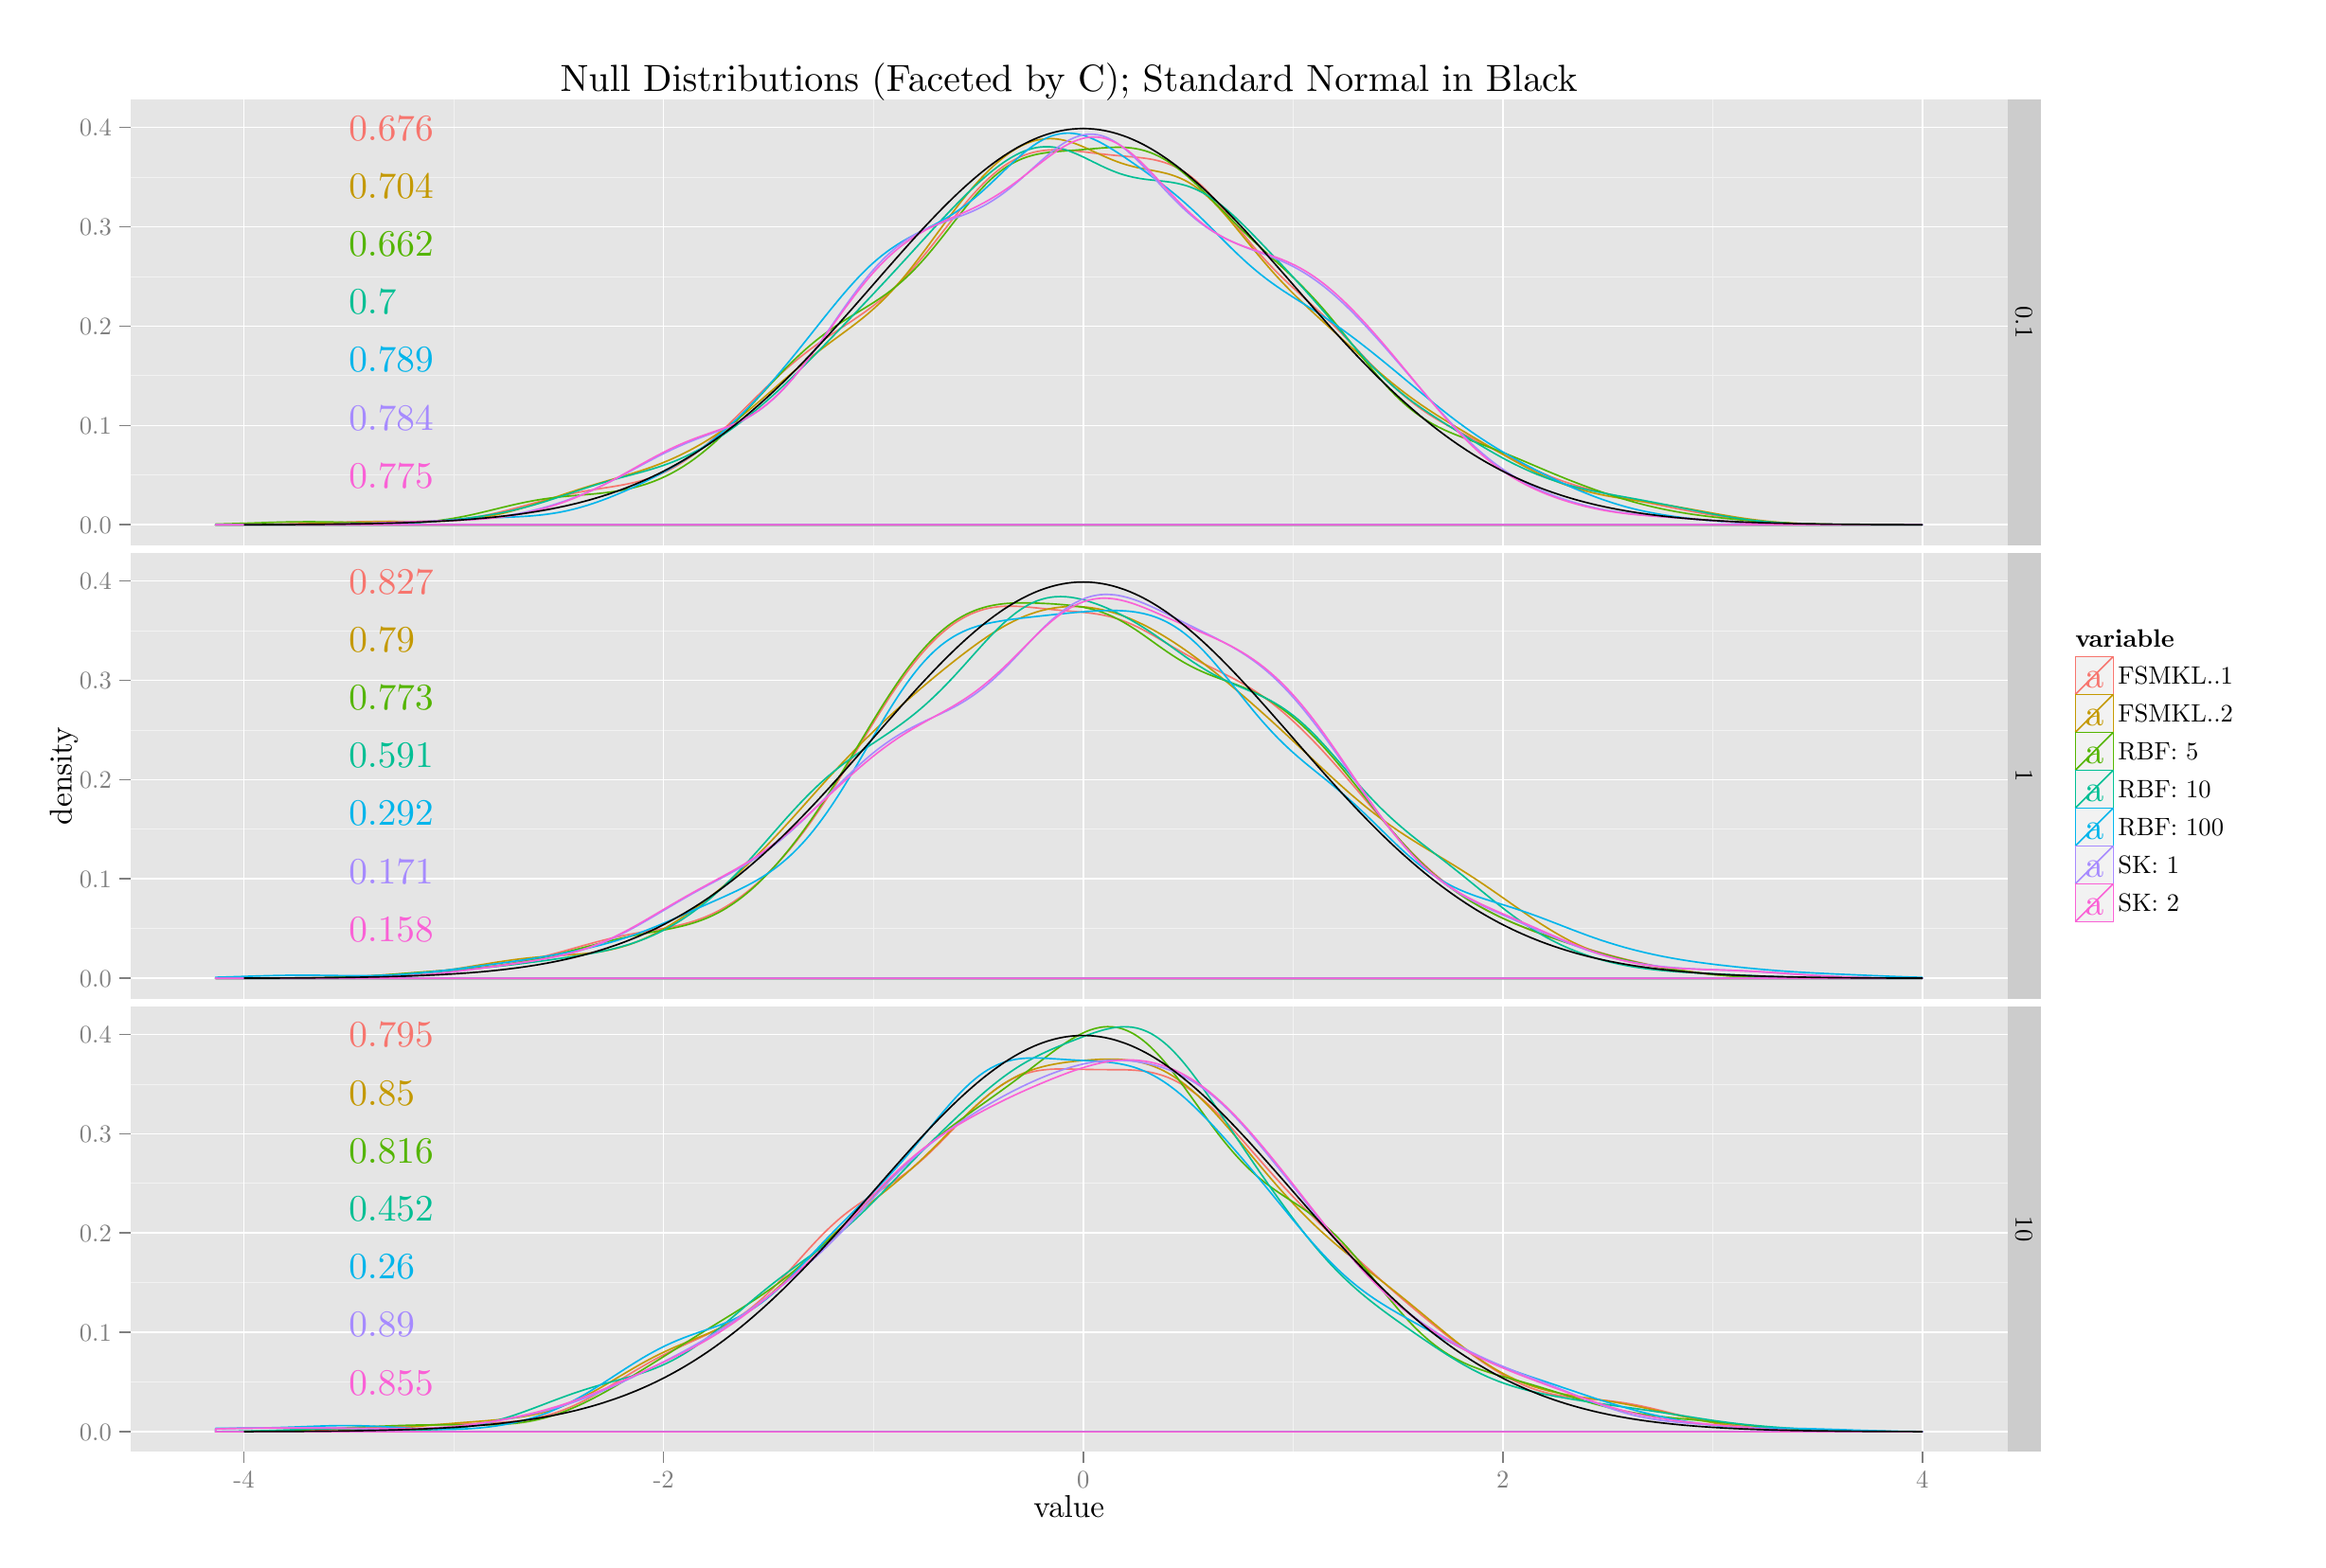
\begin{tikzpicture}[x=1pt,y=1pt]
\definecolor[named]{fillColor}{rgb}{1.00,1.00,1.00}
\path[use as bounding box,fill=fillColor,fill opacity=0.00] (0,0) rectangle (867.24,578.16);
\begin{scope}
\path[clip] (  0.00,  0.00) rectangle (867.24,578.16);
\definecolor[named]{drawColor}{rgb}{1.00,1.00,1.00}
\definecolor[named]{fillColor}{rgb}{1.00,1.00,1.00}

\path[draw=drawColor,line width= 0.6pt,line join=round,line cap=round,fill=fillColor] (  0.00, -0.00) rectangle (867.24,578.16);
\end{scope}
\begin{scope}
\path[clip] ( 39.69,380.14) rectangle (756.04,550.17);
\definecolor[named]{fillColor}{rgb}{0.90,0.90,0.90}

\path[fill=fillColor] ( 39.69,380.14) rectangle (756.04,550.17);
\definecolor[named]{drawColor}{rgb}{0.95,0.95,0.95}

\path[draw=drawColor,line width= 0.3pt,line join=round] ( 39.69,406.82) --
	(756.04,406.82);

\path[draw=drawColor,line width= 0.3pt,line join=round] ( 39.69,444.73) --
	(756.04,444.73);

\path[draw=drawColor,line width= 0.3pt,line join=round] ( 39.69,482.63) --
	(756.04,482.63);

\path[draw=drawColor,line width= 0.3pt,line join=round] ( 39.69,520.54) --
	(756.04,520.54);

\path[draw=drawColor,line width= 0.3pt,line join=round] (163.10,380.14) --
	(163.10,550.17);

\path[draw=drawColor,line width= 0.3pt,line join=round] (323.21,380.14) --
	(323.21,550.17);

\path[draw=drawColor,line width= 0.3pt,line join=round] (483.32,380.14) --
	(483.32,550.17);

\path[draw=drawColor,line width= 0.3pt,line join=round] (643.42,380.14) --
	(643.42,550.17);
\definecolor[named]{drawColor}{rgb}{1.00,1.00,1.00}

\path[draw=drawColor,line width= 0.6pt,line join=round] ( 39.69,387.86) --
	(756.04,387.86);

\path[draw=drawColor,line width= 0.6pt,line join=round] ( 39.69,425.77) --
	(756.04,425.77);

\path[draw=drawColor,line width= 0.6pt,line join=round] ( 39.69,463.68) --
	(756.04,463.68);

\path[draw=drawColor,line width= 0.6pt,line join=round] ( 39.69,501.59) --
	(756.04,501.59);

\path[draw=drawColor,line width= 0.6pt,line join=round] ( 39.69,539.50) --
	(756.04,539.50);

\path[draw=drawColor,line width= 0.6pt,line join=round] ( 83.05,380.14) --
	( 83.05,550.17);

\path[draw=drawColor,line width= 0.6pt,line join=round] (243.16,380.14) --
	(243.16,550.17);

\path[draw=drawColor,line width= 0.6pt,line join=round] (403.26,380.14) --
	(403.26,550.17);

\path[draw=drawColor,line width= 0.6pt,line join=round] (563.37,380.14) --
	(563.37,550.17);

\path[draw=drawColor,line width= 0.6pt,line join=round] (723.48,380.14) --
	(723.48,550.17);
\definecolor[named]{drawColor}{rgb}{0.97,0.46,0.43}

\path[draw=drawColor,line width= 0.6pt,line join=round,line cap=round] ( 72.25,387.88) --
	( 73.52,387.88) --
	( 74.80,387.88) --
	( 76.07,387.89) --
	( 77.35,387.89) --
	( 78.62,387.90) --
	( 79.89,387.90) --
	( 81.17,387.91) --
	( 82.44,387.92) --
	( 83.72,387.93) --
	( 84.99,387.94) --
	( 86.27,387.95) --
	( 87.54,387.96) --
	( 88.82,387.98) --
	( 90.09,388.00) --
	( 91.36,388.01) --
	( 92.64,388.03) --
	( 93.91,388.06) --
	( 95.19,388.08) --
	( 96.46,388.11) --
	( 97.74,388.14) --
	( 99.01,388.17) --
	(100.29,388.20) --
	(101.56,388.24) --
	(102.83,388.27) --
	(104.11,388.31) --
	(105.38,388.35) --
	(106.66,388.39) --
	(107.93,388.44) --
	(109.21,388.48) --
	(110.48,388.53) --
	(111.76,388.58) --
	(113.03,388.62) --
	(114.30,388.67) --
	(115.58,388.71) --
	(116.85,388.76) --
	(118.13,388.80) --
	(119.40,388.85) --
	(120.68,388.89) --
	(121.95,388.92) --
	(123.22,388.96) --
	(124.50,388.99) --
	(125.77,389.02) --
	(127.05,389.05) --
	(128.32,389.07) --
	(129.60,389.09) --
	(130.87,389.10) --
	(132.15,389.11) --
	(133.42,389.12) --
	(134.69,389.12) --
	(135.97,389.12) --
	(137.24,389.12) --
	(138.52,389.12) --
	(139.79,389.12) --
	(141.07,389.11) --
	(142.34,389.10) --
	(143.62,389.10) --
	(144.89,389.09) --
	(146.16,389.09) --
	(147.44,389.09) --
	(148.71,389.10) --
	(149.99,389.11) --
	(151.26,389.13) --
	(152.54,389.15) --
	(153.81,389.18) --
	(155.09,389.22) --
	(156.36,389.27) --
	(157.63,389.33) --
	(158.91,389.40) --
	(160.18,389.48) --
	(161.46,389.58) --
	(162.73,389.69) --
	(164.01,389.81) --
	(165.28,389.95) --
	(166.56,390.10) --
	(167.83,390.26) --
	(169.10,390.44) --
	(170.38,390.64) --
	(171.65,390.85) --
	(172.93,391.07) --
	(174.20,391.31) --
	(175.48,391.56) --
	(176.75,391.82) --
	(178.03,392.10) --
	(179.30,392.38) --
	(180.57,392.68) --
	(181.85,392.99) --
	(183.12,393.31) --
	(184.40,393.64) --
	(185.67,393.97) --
	(186.95,394.31) --
	(188.22,394.65) --
	(189.49,395.00) --
	(190.77,395.35) --
	(192.04,395.70) --
	(193.32,396.05) --
	(194.59,396.40) --
	(195.87,396.75) --
	(197.14,397.09) --
	(198.42,397.43) --
	(199.69,397.76) --
	(200.96,398.08) --
	(202.24,398.40) --
	(203.51,398.71) --
	(204.79,399.01) --
	(206.06,399.29) --
	(207.34,399.57) --
	(208.61,399.84) --
	(209.89,400.10) --
	(211.16,400.35) --
	(212.43,400.59) --
	(213.71,400.81) --
	(214.98,401.03) --
	(216.26,401.25) --
	(217.53,401.46) --
	(218.81,401.66) --
	(220.08,401.86) --
	(221.36,402.06) --
	(222.63,402.26) --
	(223.90,402.47) --
	(225.18,402.68) --
	(226.45,402.90) --
	(227.73,403.13) --
	(229.00,403.37) --
	(230.28,403.63) --
	(231.55,403.92) --
	(232.83,404.22) --
	(234.10,404.55) --
	(235.37,404.90) --
	(236.65,405.28) --
	(237.92,405.69) --
	(239.20,406.14) --
	(240.47,406.63) --
	(241.75,407.14) --
	(243.02,407.70) --
	(244.29,408.29) --
	(245.57,408.93) --
	(246.84,409.61) --
	(248.12,410.33) --
	(249.39,411.08) --
	(250.67,411.88) --
	(251.94,412.73) --
	(253.22,413.60) --
	(254.49,414.52) --
	(255.76,415.47) --
	(257.04,416.47) --
	(258.31,417.49) --
	(259.59,418.55) --
	(260.86,419.64) --
	(262.14,420.76) --
	(263.41,421.90) --
	(264.69,423.07) --
	(265.96,424.26) --
	(267.23,425.47) --
	(268.51,426.70) --
	(269.78,427.94) --
	(271.06,429.19) --
	(272.33,430.45) --
	(273.61,431.71) --
	(274.88,432.98) --
	(276.16,434.25) --
	(277.43,435.51) --
	(278.70,436.77) --
	(279.98,438.03) --
	(281.25,439.27) --
	(282.53,440.50) --
	(283.80,441.72) --
	(285.08,442.92) --
	(286.35,444.11) --
	(287.63,445.28) --
	(288.90,446.42) --
	(290.17,447.55) --
	(291.45,448.65) --
	(292.72,449.73) --
	(294.00,450.79) --
	(295.27,451.82) --
	(296.55,452.83) --
	(297.82,453.82) --
	(299.10,454.79) --
	(300.37,455.73) --
	(301.64,456.66) --
	(302.92,457.56) --
	(304.19,458.45) --
	(305.47,459.33) --
	(306.74,460.19) --
	(308.02,461.05) --
	(309.29,461.89) --
	(310.56,462.73) --
	(311.84,463.57) --
	(313.11,464.41) --
	(314.39,465.25) --
	(315.66,466.10) --
	(316.94,466.97) --
	(318.21,467.85) --
	(319.49,468.74) --
	(320.76,469.65) --
	(322.03,470.60) --
	(323.31,471.57) --
	(324.58,472.57) --
	(325.86,473.59) --
	(327.13,474.66) --
	(328.41,475.76) --
	(329.68,476.91) --
	(330.96,478.09) --
	(332.23,479.31) --
	(333.50,480.57) --
	(334.78,481.88) --
	(336.05,483.23) --
	(337.33,484.62) --
	(338.60,486.04) --
	(339.88,487.50) --
	(341.15,489.00) --
	(342.43,490.53) --
	(343.70,492.09) --
	(344.97,493.67) --
	(346.25,495.27) --
	(347.52,496.89) --
	(348.80,498.52) --
	(350.07,500.15) --
	(351.35,501.79) --
	(352.62,503.42) --
	(353.90,505.04) --
	(355.17,506.64) --
	(356.44,508.23) --
	(357.72,509.78) --
	(358.99,511.31) --
	(360.27,512.80) --
	(361.54,514.24) --
	(362.82,515.64) --
	(364.09,516.99) --
	(365.37,518.29) --
	(366.64,519.53) --
	(367.91,520.70) --
	(369.19,521.82) --
	(370.46,522.87) --
	(371.74,523.86) --
	(373.01,524.77) --
	(374.29,525.62) --
	(375.56,526.40) --
	(376.83,527.11) --
	(378.11,527.77) --
	(379.38,528.34) --
	(380.66,528.85) --
	(381.93,529.31) --
	(383.21,529.70) --
	(384.48,530.04) --
	(385.76,530.31) --
	(387.03,530.53) --
	(388.30,530.71) --
	(389.58,530.84) --
	(390.85,530.93) --
	(392.13,530.97) --
	(393.40,530.98) --
	(394.68,530.96) --
	(395.95,530.90) --
	(397.23,530.83) --
	(398.50,530.73) --
	(399.77,530.61) --
	(401.05,530.48) --
	(402.32,530.34) --
	(403.60,530.19) --
	(404.87,530.04) --
	(406.15,529.88) --
	(407.42,529.73) --
	(408.70,529.57) --
	(409.97,529.43) --
	(411.24,529.28) --
	(412.52,529.15) --
	(413.79,529.02) --
	(415.07,528.89) --
	(416.34,528.77) --
	(417.62,528.66) --
	(418.89,528.55) --
	(420.17,528.44) --
	(421.44,528.33) --
	(422.71,528.22) --
	(423.99,528.10) --
	(425.26,527.95) --
	(426.54,527.80) --
	(427.81,527.62) --
	(429.09,527.41) --
	(430.36,527.17) --
	(431.63,526.88) --
	(432.91,526.55) --
	(434.18,526.17) --
	(435.46,525.73) --
	(436.73,525.24) --
	(438.01,524.67) --
	(439.28,524.03) --
	(440.56,523.33) --
	(441.83,522.56) --
	(443.10,521.71) --
	(444.38,520.77) --
	(445.65,519.76) --
	(446.93,518.67) --
	(448.20,517.52) --
	(449.48,516.31) --
	(450.75,515.01) --
	(452.03,513.65) --
	(453.30,512.25) --
	(454.57,510.80) --
	(455.85,509.31) --
	(457.12,507.77) --
	(458.40,506.21) --
	(459.67,504.64) --
	(460.95,503.05) --
	(462.22,501.46) --
	(463.50,499.87) --
	(464.77,498.29) --
	(466.04,496.72) --
	(467.32,495.18) --
	(468.59,493.65) --
	(469.87,492.16) --
	(471.14,490.71) --
	(472.42,489.28) --
	(473.69,487.89) --
	(474.97,486.53) --
	(476.24,485.21) --
	(477.51,483.92) --
	(478.79,482.66) --
	(480.06,481.43) --
	(481.34,480.22) --
	(482.61,479.03) --
	(483.89,477.86) --
	(485.16,476.70) --
	(486.44,475.55) --
	(487.71,474.39) --
	(488.98,473.24) --
	(490.26,472.09) --
	(491.53,470.92) --
	(492.81,469.74) --
	(494.08,468.56) --
	(495.36,467.35) --
	(496.63,466.12) --
	(497.90,464.88) --
	(499.18,463.63) --
	(500.45,462.35) --
	(501.73,461.06) --
	(503.00,459.75) --
	(504.28,458.43) --
	(505.55,457.10) --
	(506.83,455.76) --
	(508.10,454.42) --
	(509.37,453.07) --
	(510.65,451.73) --
	(511.92,450.39) --
	(513.20,449.06) --
	(514.47,447.74) --
	(515.75,446.44) --
	(517.02,445.16) --
	(518.30,443.90) --
	(519.57,442.66) --
	(520.84,441.45) --
	(522.12,440.27) --
	(523.39,439.12) --
	(524.67,438.00) --
	(525.94,436.92) --
	(527.22,435.86) --
	(528.49,434.85) --
	(529.77,433.87) --
	(531.04,432.92) --
	(532.31,432.00) --
	(533.59,431.12) --
	(534.86,430.26) --
	(536.14,429.44) --
	(537.41,428.64) --
	(538.69,427.86) --
	(539.96,427.11) --
	(541.24,426.38) --
	(542.51,425.67) --
	(543.78,424.97) --
	(545.06,424.28) --
	(546.33,423.60) --
	(547.61,422.94) --
	(548.88,422.28) --
	(550.16,421.62) --
	(551.43,420.97) --
	(552.71,420.32) --
	(553.98,419.67) --
	(555.25,419.02) --
	(556.53,418.36) --
	(557.80,417.71) --
	(559.08,417.06) --
	(560.35,416.41) --
	(561.63,415.75) --
	(562.90,415.10) --
	(564.17,414.45) --
	(565.45,413.80) --
	(566.72,413.15) --
	(568.00,412.51) --
	(569.27,411.88) --
	(570.55,411.25) --
	(571.82,410.63) --
	(573.10,410.02) --
	(574.37,409.42) --
	(575.64,408.84) --
	(576.92,408.27) --
	(578.19,407.71) --
	(579.47,407.17) --
	(580.74,406.64) --
	(582.02,406.13) --
	(583.29,405.64) --
	(584.57,405.16) --
	(585.84,404.70) --
	(587.11,404.25) --
	(588.39,403.82) --
	(589.66,403.40) --
	(590.94,403.00) --
	(592.21,402.62) --
	(593.49,402.24) --
	(594.76,401.88) --
	(596.04,401.53) --
	(597.31,401.19) --
	(598.58,400.85) --
	(599.86,400.53) --
	(601.13,400.21) --
	(602.41,399.90) --
	(603.68,399.60) --
	(604.96,399.30) --
	(606.23,399.00) --
	(607.51,398.71) --
	(608.78,398.43) --
	(610.05,398.14) --
	(611.33,397.86) --
	(612.60,397.59) --
	(613.88,397.31) --
	(615.15,397.04) --
	(616.43,396.76) --
	(617.70,396.49) --
	(618.97,396.23) --
	(620.25,395.96) --
	(621.52,395.70) --
	(622.80,395.44) --
	(624.07,395.18) --
	(625.35,394.92) --
	(626.62,394.67) --
	(627.90,394.41) --
	(629.17,394.16) --
	(630.44,393.92) --
	(631.72,393.67) --
	(632.99,393.43) --
	(634.27,393.19) --
	(635.54,392.95) --
	(636.82,392.72) --
	(638.09,392.48) --
	(639.37,392.26) --
	(640.64,392.03) --
	(641.91,391.81) --
	(643.19,391.60) --
	(644.46,391.39) --
	(645.74,391.18) --
	(647.01,390.98) --
	(648.29,390.78) --
	(649.56,390.59) --
	(650.84,390.41) --
	(652.11,390.23) --
	(653.38,390.06) --
	(654.66,389.90) --
	(655.93,389.74) --
	(657.21,389.59) --
	(658.48,389.45) --
	(659.76,389.31) --
	(661.03,389.18) --
	(662.31,389.06) --
	(663.58,388.95) --
	(664.85,388.85) --
	(666.13,388.75) --
	(667.40,388.66) --
	(668.68,388.57) --
	(669.95,388.50) --
	(671.23,388.43) --
	(672.50,388.36) --
	(673.78,388.30) --
	(675.05,388.25) --
	(676.32,388.20) --
	(677.60,388.16) --
	(678.87,388.12) --
	(680.15,388.09) --
	(681.42,388.06) --
	(682.70,388.03) --
	(683.97,388.01) --
	(685.24,387.98) --
	(686.52,387.97) --
	(687.79,387.95) --
	(689.07,387.94) --
	(690.34,387.93) --
	(691.62,387.92) --
	(692.89,387.91) --
	(694.17,387.90) --
	(695.44,387.89) --
	(696.71,387.89) --
	(697.99,387.88) --
	(699.26,387.88) --
	(700.54,387.88) --
	(701.81,387.88) --
	(703.09,387.87) --
	(704.36,387.87) --
	(705.64,387.87) --
	(706.91,387.87) --
	(708.18,387.87) --
	(709.46,387.87) --
	(710.73,387.87) --
	(712.01,387.87) --
	(713.28,387.87) --
	(714.56,387.87) --
	(715.83,387.87) --
	(717.11,387.87) --
	(718.38,387.87) --
	(719.65,387.87) --
	(720.93,387.86) --
	(722.20,387.86) --
	(723.48,387.86) --
	(723.48,387.86) --
	(722.20,387.86) --
	(720.93,387.86) --
	(719.65,387.86) --
	(718.38,387.86) --
	(717.11,387.86) --
	(715.83,387.86) --
	(714.56,387.86) --
	(713.28,387.86) --
	(712.01,387.86) --
	(710.73,387.86) --
	(709.46,387.86) --
	(708.18,387.86) --
	(706.91,387.86) --
	(705.64,387.86) --
	(704.36,387.86) --
	(703.09,387.86) --
	(701.81,387.86) --
	(700.54,387.86) --
	(699.26,387.86) --
	(697.99,387.86) --
	(696.71,387.86) --
	(695.44,387.86) --
	(694.17,387.86) --
	(692.89,387.86) --
	(691.62,387.86) --
	(690.34,387.86) --
	(689.07,387.86) --
	(687.79,387.86) --
	(686.52,387.86) --
	(685.24,387.86) --
	(683.97,387.86) --
	(682.70,387.86) --
	(681.42,387.86) --
	(680.15,387.86) --
	(678.87,387.86) --
	(677.60,387.86) --
	(676.32,387.86) --
	(675.05,387.86) --
	(673.78,387.86) --
	(672.50,387.86) --
	(671.23,387.86) --
	(669.95,387.86) --
	(668.68,387.86) --
	(667.40,387.86) --
	(666.13,387.86) --
	(664.85,387.86) --
	(663.58,387.86) --
	(662.31,387.86) --
	(661.03,387.86) --
	(659.76,387.86) --
	(658.48,387.86) --
	(657.21,387.86) --
	(655.93,387.86) --
	(654.66,387.86) --
	(653.38,387.86) --
	(652.11,387.86) --
	(650.84,387.86) --
	(649.56,387.86) --
	(648.29,387.86) --
	(647.01,387.86) --
	(645.74,387.86) --
	(644.46,387.86) --
	(643.19,387.86) --
	(641.91,387.86) --
	(640.64,387.86) --
	(639.37,387.86) --
	(638.09,387.86) --
	(636.82,387.86) --
	(635.54,387.86) --
	(634.27,387.86) --
	(632.99,387.86) --
	(631.72,387.86) --
	(630.44,387.86) --
	(629.17,387.86) --
	(627.90,387.86) --
	(626.62,387.86) --
	(625.35,387.86) --
	(624.07,387.86) --
	(622.80,387.86) --
	(621.52,387.86) --
	(620.25,387.86) --
	(618.97,387.86) --
	(617.70,387.86) --
	(616.43,387.86) --
	(615.15,387.86) --
	(613.88,387.86) --
	(612.60,387.86) --
	(611.33,387.86) --
	(610.05,387.86) --
	(608.78,387.86) --
	(607.51,387.86) --
	(606.23,387.86) --
	(604.96,387.86) --
	(603.68,387.86) --
	(602.41,387.86) --
	(601.13,387.86) --
	(599.86,387.86) --
	(598.58,387.86) --
	(597.31,387.86) --
	(596.04,387.86) --
	(594.76,387.86) --
	(593.49,387.86) --
	(592.21,387.86) --
	(590.94,387.86) --
	(589.66,387.86) --
	(588.39,387.86) --
	(587.11,387.86) --
	(585.84,387.86) --
	(584.57,387.86) --
	(583.29,387.86) --
	(582.02,387.86) --
	(580.74,387.86) --
	(579.47,387.86) --
	(578.19,387.86) --
	(576.92,387.86) --
	(575.64,387.86) --
	(574.37,387.86) --
	(573.10,387.86) --
	(571.82,387.86) --
	(570.55,387.86) --
	(569.27,387.86) --
	(568.00,387.86) --
	(566.72,387.86) --
	(565.45,387.86) --
	(564.17,387.86) --
	(562.90,387.86) --
	(561.63,387.86) --
	(560.35,387.86) --
	(559.08,387.86) --
	(557.80,387.86) --
	(556.53,387.86) --
	(555.25,387.86) --
	(553.98,387.86) --
	(552.71,387.86) --
	(551.43,387.86) --
	(550.16,387.86) --
	(548.88,387.86) --
	(547.61,387.86) --
	(546.33,387.86) --
	(545.06,387.86) --
	(543.78,387.86) --
	(542.51,387.86) --
	(541.24,387.86) --
	(539.96,387.86) --
	(538.69,387.86) --
	(537.41,387.86) --
	(536.14,387.86) --
	(534.86,387.86) --
	(533.59,387.86) --
	(532.31,387.86) --
	(531.04,387.86) --
	(529.77,387.86) --
	(528.49,387.86) --
	(527.22,387.86) --
	(525.94,387.86) --
	(524.67,387.86) --
	(523.39,387.86) --
	(522.12,387.86) --
	(520.84,387.86) --
	(519.57,387.86) --
	(518.30,387.86) --
	(517.02,387.86) --
	(515.75,387.86) --
	(514.47,387.86) --
	(513.20,387.86) --
	(511.92,387.86) --
	(510.65,387.86) --
	(509.37,387.86) --
	(508.10,387.86) --
	(506.83,387.86) --
	(505.55,387.86) --
	(504.28,387.86) --
	(503.00,387.86) --
	(501.73,387.86) --
	(500.45,387.86) --
	(499.18,387.86) --
	(497.90,387.86) --
	(496.63,387.86) --
	(495.36,387.86) --
	(494.08,387.86) --
	(492.81,387.86) --
	(491.53,387.86) --
	(490.26,387.86) --
	(488.98,387.86) --
	(487.71,387.86) --
	(486.44,387.86) --
	(485.16,387.86) --
	(483.89,387.86) --
	(482.61,387.86) --
	(481.34,387.86) --
	(480.06,387.86) --
	(478.79,387.86) --
	(477.51,387.86) --
	(476.24,387.86) --
	(474.97,387.86) --
	(473.69,387.86) --
	(472.42,387.86) --
	(471.14,387.86) --
	(469.87,387.86) --
	(468.59,387.86) --
	(467.32,387.86) --
	(466.04,387.86) --
	(464.77,387.86) --
	(463.50,387.86) --
	(462.22,387.86) --
	(460.95,387.86) --
	(459.67,387.86) --
	(458.40,387.86) --
	(457.12,387.86) --
	(455.85,387.86) --
	(454.57,387.86) --
	(453.30,387.86) --
	(452.03,387.86) --
	(450.75,387.86) --
	(449.48,387.86) --
	(448.20,387.86) --
	(446.93,387.86) --
	(445.65,387.86) --
	(444.38,387.86) --
	(443.10,387.86) --
	(441.83,387.86) --
	(440.56,387.86) --
	(439.28,387.86) --
	(438.01,387.86) --
	(436.73,387.86) --
	(435.46,387.86) --
	(434.18,387.86) --
	(432.91,387.86) --
	(431.63,387.86) --
	(430.36,387.86) --
	(429.09,387.86) --
	(427.81,387.86) --
	(426.54,387.86) --
	(425.26,387.86) --
	(423.99,387.86) --
	(422.71,387.86) --
	(421.44,387.86) --
	(420.17,387.86) --
	(418.89,387.86) --
	(417.62,387.86) --
	(416.34,387.86) --
	(415.07,387.86) --
	(413.79,387.86) --
	(412.52,387.86) --
	(411.24,387.86) --
	(409.97,387.86) --
	(408.70,387.86) --
	(407.42,387.86) --
	(406.15,387.86) --
	(404.87,387.86) --
	(403.60,387.86) --
	(402.32,387.86) --
	(401.05,387.86) --
	(399.77,387.86) --
	(398.50,387.86) --
	(397.23,387.86) --
	(395.95,387.86) --
	(394.68,387.86) --
	(393.40,387.86) --
	(392.13,387.86) --
	(390.85,387.86) --
	(389.58,387.86) --
	(388.30,387.86) --
	(387.03,387.86) --
	(385.76,387.86) --
	(384.48,387.86) --
	(383.21,387.86) --
	(381.93,387.86) --
	(380.66,387.86) --
	(379.38,387.86) --
	(378.11,387.86) --
	(376.83,387.86) --
	(375.56,387.86) --
	(374.29,387.86) --
	(373.01,387.86) --
	(371.74,387.86) --
	(370.46,387.86) --
	(369.19,387.86) --
	(367.91,387.86) --
	(366.64,387.86) --
	(365.37,387.86) --
	(364.09,387.86) --
	(362.82,387.86) --
	(361.54,387.86) --
	(360.27,387.86) --
	(358.99,387.86) --
	(357.72,387.86) --
	(356.44,387.86) --
	(355.17,387.86) --
	(353.90,387.86) --
	(352.62,387.86) --
	(351.35,387.86) --
	(350.07,387.86) --
	(348.80,387.86) --
	(347.52,387.86) --
	(346.25,387.86) --
	(344.97,387.86) --
	(343.70,387.86) --
	(342.43,387.86) --
	(341.15,387.86) --
	(339.88,387.86) --
	(338.60,387.86) --
	(337.33,387.86) --
	(336.05,387.86) --
	(334.78,387.86) --
	(333.50,387.86) --
	(332.23,387.86) --
	(330.96,387.86) --
	(329.68,387.86) --
	(328.41,387.86) --
	(327.13,387.86) --
	(325.86,387.86) --
	(324.58,387.86) --
	(323.31,387.86) --
	(322.03,387.86) --
	(320.76,387.86) --
	(319.49,387.86) --
	(318.21,387.86) --
	(316.94,387.86) --
	(315.66,387.86) --
	(314.39,387.86) --
	(313.11,387.86) --
	(311.84,387.86) --
	(310.56,387.86) --
	(309.29,387.86) --
	(308.02,387.86) --
	(306.74,387.86) --
	(305.47,387.86) --
	(304.19,387.86) --
	(302.92,387.86) --
	(301.64,387.86) --
	(300.37,387.86) --
	(299.10,387.86) --
	(297.82,387.86) --
	(296.55,387.86) --
	(295.27,387.86) --
	(294.00,387.86) --
	(292.72,387.86) --
	(291.45,387.86) --
	(290.17,387.86) --
	(288.90,387.86) --
	(287.63,387.86) --
	(286.35,387.86) --
	(285.08,387.86) --
	(283.80,387.86) --
	(282.53,387.86) --
	(281.25,387.86) --
	(279.98,387.86) --
	(278.70,387.86) --
	(277.43,387.86) --
	(276.16,387.86) --
	(274.88,387.86) --
	(273.61,387.86) --
	(272.33,387.86) --
	(271.06,387.86) --
	(269.78,387.86) --
	(268.51,387.86) --
	(267.23,387.86) --
	(265.96,387.86) --
	(264.69,387.86) --
	(263.41,387.86) --
	(262.14,387.86) --
	(260.86,387.86) --
	(259.59,387.86) --
	(258.31,387.86) --
	(257.04,387.86) --
	(255.76,387.86) --
	(254.49,387.86) --
	(253.22,387.86) --
	(251.94,387.86) --
	(250.67,387.86) --
	(249.39,387.86) --
	(248.12,387.86) --
	(246.84,387.86) --
	(245.57,387.86) --
	(244.29,387.86) --
	(243.02,387.86) --
	(241.75,387.86) --
	(240.47,387.86) --
	(239.20,387.86) --
	(237.92,387.86) --
	(236.65,387.86) --
	(235.37,387.86) --
	(234.10,387.86) --
	(232.83,387.86) --
	(231.55,387.86) --
	(230.28,387.86) --
	(229.00,387.86) --
	(227.73,387.86) --
	(226.45,387.86) --
	(225.18,387.86) --
	(223.90,387.86) --
	(222.63,387.86) --
	(221.36,387.86) --
	(220.08,387.86) --
	(218.81,387.86) --
	(217.53,387.86) --
	(216.26,387.86) --
	(214.98,387.86) --
	(213.71,387.86) --
	(212.43,387.86) --
	(211.16,387.86) --
	(209.89,387.86) --
	(208.61,387.86) --
	(207.34,387.86) --
	(206.06,387.86) --
	(204.79,387.86) --
	(203.51,387.86) --
	(202.24,387.86) --
	(200.96,387.86) --
	(199.69,387.86) --
	(198.42,387.86) --
	(197.14,387.86) --
	(195.87,387.86) --
	(194.59,387.86) --
	(193.32,387.86) --
	(192.04,387.86) --
	(190.77,387.86) --
	(189.49,387.86) --
	(188.22,387.86) --
	(186.95,387.86) --
	(185.67,387.86) --
	(184.40,387.86) --
	(183.12,387.86) --
	(181.85,387.86) --
	(180.57,387.86) --
	(179.30,387.86) --
	(178.03,387.86) --
	(176.75,387.86) --
	(175.48,387.86) --
	(174.20,387.86) --
	(172.93,387.86) --
	(171.65,387.86) --
	(170.38,387.86) --
	(169.10,387.86) --
	(167.83,387.86) --
	(166.56,387.86) --
	(165.28,387.86) --
	(164.01,387.86) --
	(162.73,387.86) --
	(161.46,387.86) --
	(160.18,387.86) --
	(158.91,387.86) --
	(157.63,387.86) --
	(156.36,387.86) --
	(155.09,387.86) --
	(153.81,387.86) --
	(152.54,387.86) --
	(151.26,387.86) --
	(149.99,387.86) --
	(148.71,387.86) --
	(147.44,387.86) --
	(146.16,387.86) --
	(144.89,387.86) --
	(143.62,387.86) --
	(142.34,387.86) --
	(141.07,387.86) --
	(139.79,387.86) --
	(138.52,387.86) --
	(137.24,387.86) --
	(135.97,387.86) --
	(134.69,387.86) --
	(133.42,387.86) --
	(132.15,387.86) --
	(130.87,387.86) --
	(129.60,387.86) --
	(128.32,387.86) --
	(127.05,387.86) --
	(125.77,387.86) --
	(124.50,387.86) --
	(123.22,387.86) --
	(121.95,387.86) --
	(120.68,387.86) --
	(119.40,387.86) --
	(118.13,387.86) --
	(116.85,387.86) --
	(115.58,387.86) --
	(114.30,387.86) --
	(113.03,387.86) --
	(111.76,387.86) --
	(110.48,387.86) --
	(109.21,387.86) --
	(107.93,387.86) --
	(106.66,387.86) --
	(105.38,387.86) --
	(104.11,387.86) --
	(102.83,387.86) --
	(101.56,387.86) --
	(100.29,387.86) --
	( 99.01,387.86) --
	( 97.74,387.86) --
	( 96.46,387.86) --
	( 95.19,387.86) --
	( 93.91,387.86) --
	( 92.64,387.86) --
	( 91.36,387.86) --
	( 90.09,387.86) --
	( 88.82,387.86) --
	( 87.54,387.86) --
	( 86.27,387.86) --
	( 84.99,387.86) --
	( 83.72,387.86) --
	( 82.44,387.86) --
	( 81.17,387.86) --
	( 79.89,387.86) --
	( 78.62,387.86) --
	( 77.35,387.86) --
	( 76.07,387.86) --
	( 74.80,387.86) --
	( 73.52,387.86) --
	( 72.25,387.86) --
	( 72.25,387.88);
\definecolor[named]{drawColor}{rgb}{0.77,0.60,0.00}

\path[draw=drawColor,line width= 0.6pt,line join=round,line cap=round] ( 72.25,387.87) --
	( 73.52,387.87) --
	( 74.80,387.87) --
	( 76.07,387.87) --
	( 77.35,387.87) --
	( 78.62,387.88) --
	( 79.89,387.88) --
	( 81.17,387.88) --
	( 82.44,387.89) --
	( 83.72,387.89) --
	( 84.99,387.90) --
	( 86.27,387.90) --
	( 87.54,387.91) --
	( 88.82,387.91) --
	( 90.09,387.92) --
	( 91.36,387.93) --
	( 92.64,387.94) --
	( 93.91,387.96) --
	( 95.19,387.97) --
	( 96.46,387.99) --
	( 97.74,388.00) --
	( 99.01,388.02) --
	(100.29,388.04) --
	(101.56,388.07) --
	(102.83,388.09) --
	(104.11,388.12) --
	(105.38,388.15) --
	(106.66,388.18) --
	(107.93,388.21) --
	(109.21,388.25) --
	(110.48,388.28) --
	(111.76,388.32) --
	(113.03,388.37) --
	(114.30,388.41) --
	(115.58,388.45) --
	(116.85,388.50) --
	(118.13,388.54) --
	(119.40,388.59) --
	(120.68,388.63) --
	(121.95,388.68) --
	(123.22,388.73) --
	(124.50,388.77) --
	(125.77,388.81) --
	(127.05,388.86) --
	(128.32,388.90) --
	(129.60,388.93) --
	(130.87,388.97) --
	(132.15,389.00) --
	(133.42,389.03) --
	(134.69,389.06) --
	(135.97,389.08) --
	(137.24,389.10) --
	(138.52,389.12) --
	(139.79,389.13) --
	(141.07,389.14) --
	(142.34,389.15) --
	(143.62,389.15) --
	(144.89,389.16) --
	(146.16,389.16) --
	(147.44,389.17) --
	(148.71,389.17) --
	(149.99,389.17) --
	(151.26,389.18) --
	(152.54,389.19) --
	(153.81,389.20) --
	(155.09,389.22) --
	(156.36,389.25) --
	(157.63,389.28) --
	(158.91,389.31) --
	(160.18,389.36) --
	(161.46,389.42) --
	(162.73,389.49) --
	(164.01,389.57) --
	(165.28,389.66) --
	(166.56,389.76) --
	(167.83,389.88) --
	(169.10,390.02) --
	(170.38,390.17) --
	(171.65,390.33) --
	(172.93,390.51) --
	(174.20,390.71) --
	(175.48,390.93) --
	(176.75,391.16) --
	(178.03,391.41) --
	(179.30,391.67) --
	(180.57,391.96) --
	(181.85,392.26) --
	(183.12,392.57) --
	(184.40,392.90) --
	(185.67,393.24) --
	(186.95,393.60) --
	(188.22,393.96) --
	(189.49,394.35) --
	(190.77,394.74) --
	(192.04,395.13) --
	(193.32,395.54) --
	(194.59,395.96) --
	(195.87,396.38) --
	(197.14,396.80) --
	(198.42,397.23) --
	(199.69,397.66) --
	(200.96,398.10) --
	(202.24,398.53) --
	(203.51,398.96) --
	(204.79,399.39) --
	(206.06,399.81) --
	(207.34,400.24) --
	(208.61,400.65) --
	(209.89,401.07) --
	(211.16,401.48) --
	(212.43,401.88) --
	(213.71,402.27) --
	(214.98,402.67) --
	(216.26,403.05) --
	(217.53,403.44) --
	(218.81,403.81) --
	(220.08,404.19) --
	(221.36,404.56) --
	(222.63,404.93) --
	(223.90,405.30) --
	(225.18,405.67) --
	(226.45,406.04) --
	(227.73,406.42) --
	(229.00,406.80) --
	(230.28,407.18) --
	(231.55,407.58) --
	(232.83,407.98) --
	(234.10,408.39) --
	(235.37,408.81) --
	(236.65,409.24) --
	(237.92,409.68) --
	(239.20,410.14) --
	(240.47,410.62) --
	(241.75,411.10) --
	(243.02,411.61) --
	(244.29,412.13) --
	(245.57,412.67) --
	(246.84,413.23) --
	(248.12,413.81) --
	(249.39,414.41) --
	(250.67,415.03) --
	(251.94,415.67) --
	(253.22,416.33) --
	(254.49,417.01) --
	(255.76,417.71) --
	(257.04,418.43) --
	(258.31,419.18) --
	(259.59,419.96) --
	(260.86,420.75) --
	(262.14,421.56) --
	(263.41,422.40) --
	(264.69,423.26) --
	(265.96,424.15) --
	(267.23,425.05) --
	(268.51,425.98) --
	(269.78,426.92) --
	(271.06,427.90) --
	(272.33,428.89) --
	(273.61,429.90) --
	(274.88,430.93) --
	(276.16,431.97) --
	(277.43,433.03) --
	(278.70,434.11) --
	(279.98,435.20) --
	(281.25,436.29) --
	(282.53,437.40) --
	(283.80,438.51) --
	(285.08,439.63) --
	(286.35,440.74) --
	(287.63,441.86) --
	(288.90,442.97) --
	(290.17,444.08) --
	(291.45,445.18) --
	(292.72,446.28) --
	(294.00,447.36) --
	(295.27,448.43) --
	(296.55,449.49) --
	(297.82,450.53) --
	(299.10,451.56) --
	(300.37,452.57) --
	(301.64,453.57) --
	(302.92,454.55) --
	(304.19,455.52) --
	(305.47,456.48) --
	(306.74,457.43) --
	(308.02,458.37) --
	(309.29,459.31) --
	(310.56,460.24) --
	(311.84,461.18) --
	(313.11,462.12) --
	(314.39,463.07) --
	(315.66,464.03) --
	(316.94,465.01) --
	(318.21,466.01) --
	(319.49,467.03) --
	(320.76,468.08) --
	(322.03,469.17) --
	(323.31,470.30) --
	(324.58,471.46) --
	(325.86,472.65) --
	(327.13,473.89) --
	(328.41,475.18) --
	(329.68,476.52) --
	(330.96,477.90) --
	(332.23,479.32) --
	(333.50,480.78) --
	(334.78,482.29) --
	(336.05,483.85) --
	(337.33,485.44) --
	(338.60,487.06) --
	(339.88,488.71) --
	(341.15,490.39) --
	(342.43,492.09) --
	(343.70,493.81) --
	(344.97,495.54) --
	(346.25,497.28) --
	(347.52,499.02) --
	(348.80,500.76) --
	(350.07,502.49) --
	(351.35,504.21) --
	(352.62,505.92) --
	(353.90,507.60) --
	(355.17,509.25) --
	(356.44,510.88) --
	(357.72,512.48) --
	(358.99,514.04) --
	(360.27,515.56) --
	(361.54,517.04) --
	(362.82,518.48) --
	(364.09,519.87) --
	(365.37,521.22) --
	(366.64,522.51) --
	(367.91,523.75) --
	(369.19,524.94) --
	(370.46,526.07) --
	(371.74,527.16) --
	(373.01,528.17) --
	(374.29,529.13) --
	(375.56,530.02) --
	(376.83,530.85) --
	(378.11,531.62) --
	(379.38,532.32) --
	(380.66,532.94) --
	(381.93,533.49) --
	(383.21,533.97) --
	(384.48,534.38) --
	(385.76,534.71) --
	(387.03,534.95) --
	(388.30,535.13) --
	(389.58,535.23) --
	(390.85,535.26) --
	(392.13,535.21) --
	(393.40,535.08) --
	(394.68,534.89) --
	(395.95,534.63) --
	(397.23,534.32) --
	(398.50,533.95) --
	(399.77,533.52) --
	(401.05,533.04) --
	(402.32,532.54) --
	(403.60,532.00) --
	(404.87,531.44) --
	(406.15,530.85) --
	(407.42,530.26) --
	(408.70,529.67) --
	(409.97,529.08) --
	(411.24,528.51) --
	(412.52,527.95) --
	(413.79,527.41) --
	(415.07,526.90) --
	(416.34,526.41) --
	(417.62,525.96) --
	(418.89,525.55) --
	(420.17,525.17) --
	(421.44,524.82) --
	(422.71,524.50) --
	(423.99,524.20) --
	(425.26,523.94) --
	(426.54,523.69) --
	(427.81,523.45) --
	(429.09,523.21) --
	(430.36,522.98) --
	(431.63,522.73) --
	(432.91,522.46) --
	(434.18,522.17) --
	(435.46,521.85) --
	(436.73,521.48) --
	(438.01,521.06) --
	(439.28,520.58) --
	(440.56,520.04) --
	(441.83,519.45) --
	(443.10,518.78) --
	(444.38,518.02) --
	(445.65,517.19) --
	(446.93,516.29) --
	(448.20,515.31) --
	(449.48,514.26) --
	(450.75,513.13) --
	(452.03,511.92) --
	(453.30,510.66) --
	(454.57,509.34) --
	(455.85,507.96) --
	(457.12,506.53) --
	(458.40,505.06) --
	(459.67,503.56) --
	(460.95,502.02) --
	(462.22,500.47) --
	(463.50,498.90) --
	(464.77,497.33) --
	(466.04,495.75) --
	(467.32,494.18) --
	(468.59,492.62) --
	(469.87,491.07) --
	(471.14,489.55) --
	(472.42,488.04) --
	(473.69,486.56) --
	(474.97,485.10) --
	(476.24,483.68) --
	(477.51,482.28) --
	(478.79,480.90) --
	(480.06,479.56) --
	(481.34,478.24) --
	(482.61,476.94) --
	(483.89,475.67) --
	(485.16,474.42) --
	(486.44,473.19) --
	(487.71,471.97) --
	(488.98,470.77) --
	(490.26,469.58) --
	(491.53,468.40) --
	(492.81,467.22) --
	(494.08,466.05) --
	(495.36,464.89) --
	(496.63,463.73) --
	(497.90,462.57) --
	(499.18,461.41) --
	(500.45,460.25) --
	(501.73,459.09) --
	(503.00,457.93) --
	(504.28,456.77) --
	(505.55,455.61) --
	(506.83,454.46) --
	(508.10,453.31) --
	(509.37,452.16) --
	(510.65,451.02) --
	(511.92,449.88) --
	(513.20,448.75) --
	(514.47,447.64) --
	(515.75,446.53) --
	(517.02,445.44) --
	(518.30,444.36) --
	(519.57,443.29) --
	(520.84,442.25) --
	(522.12,441.22) --
	(523.39,440.20) --
	(524.67,439.21) --
	(525.94,438.23) --
	(527.22,437.27) --
	(528.49,436.33) --
	(529.77,435.41) --
	(531.04,434.51) --
	(532.31,433.62) --
	(533.59,432.76) --
	(534.86,431.90) --
	(536.14,431.07) --
	(537.41,430.24) --
	(538.69,429.43) --
	(539.96,428.63) --
	(541.24,427.84) --
	(542.51,427.06) --
	(543.78,426.29) --
	(545.06,425.52) --
	(546.33,424.76) --
	(547.61,424.00) --
	(548.88,423.25) --
	(550.16,422.49) --
	(551.43,421.74) --
	(552.71,420.99) --
	(553.98,420.25) --
	(555.25,419.50) --
	(556.53,418.75) --
	(557.80,418.01) --
	(559.08,417.26) --
	(560.35,416.52) --
	(561.63,415.78) --
	(562.90,415.05) --
	(564.17,414.32) --
	(565.45,413.59) --
	(566.72,412.87) --
	(568.00,412.16) --
	(569.27,411.46) --
	(570.55,410.77) --
	(571.82,410.09) --
	(573.10,409.42) --
	(574.37,408.77) --
	(575.64,408.13) --
	(576.92,407.50) --
	(578.19,406.90) --
	(579.47,406.31) --
	(580.74,405.74) --
	(582.02,405.19) --
	(583.29,404.66) --
	(584.57,404.15) --
	(585.84,403.67) --
	(587.11,403.20) --
	(588.39,402.75) --
	(589.66,402.32) --
	(590.94,401.91) --
	(592.21,401.53) --
	(593.49,401.16) --
	(594.76,400.81) --
	(596.04,400.48) --
	(597.31,400.16) --
	(598.58,399.87) --
	(599.86,399.58) --
	(601.13,399.32) --
	(602.41,399.06) --
	(603.68,398.82) --
	(604.96,398.59) --
	(606.23,398.37) --
	(607.51,398.16) --
	(608.78,397.95) --
	(610.05,397.75) --
	(611.33,397.56) --
	(612.60,397.37) --
	(613.88,397.19) --
	(615.15,397.00) --
	(616.43,396.82) --
	(617.70,396.63) --
	(618.97,396.45) --
	(620.25,396.26) --
	(621.52,396.07) --
	(622.80,395.88) --
	(624.07,395.69) --
	(625.35,395.49) --
	(626.62,395.29) --
	(627.90,395.08) --
	(629.17,394.87) --
	(630.44,394.65) --
	(631.72,394.43) --
	(632.99,394.21) --
	(634.27,393.99) --
	(635.54,393.76) --
	(636.82,393.53) --
	(638.09,393.30) --
	(639.37,393.07) --
	(640.64,392.83) --
	(641.91,392.60) --
	(643.19,392.37) --
	(644.46,392.14) --
	(645.74,391.91) --
	(647.01,391.69) --
	(648.29,391.47) --
	(649.56,391.26) --
	(650.84,391.05) --
	(652.11,390.84) --
	(653.38,390.64) --
	(654.66,390.45) --
	(655.93,390.27) --
	(657.21,390.09) --
	(658.48,389.92) --
	(659.76,389.76) --
	(661.03,389.60) --
	(662.31,389.46) --
	(663.58,389.32) --
	(664.85,389.19) --
	(666.13,389.07) --
	(667.40,388.95) --
	(668.68,388.85) --
	(669.95,388.75) --
	(671.23,388.66) --
	(672.50,388.57) --
	(673.78,388.50) --
	(675.05,388.43) --
	(676.32,388.36) --
	(677.60,388.31) --
	(678.87,388.25) --
	(680.15,388.20) --
	(681.42,388.16) --
	(682.70,388.12) --
	(683.97,388.09) --
	(685.24,388.06) --
	(686.52,388.03) --
	(687.79,388.01) --
	(689.07,387.99) --
	(690.34,387.97) --
	(691.62,387.96) --
	(692.89,387.94) --
	(694.17,387.93) --
	(695.44,387.92) --
	(696.71,387.91) --
	(697.99,387.90) --
	(699.26,387.90) --
	(700.54,387.89) --
	(701.81,387.89) --
	(703.09,387.88) --
	(704.36,387.88) --
	(705.64,387.88) --
	(706.91,387.87) --
	(708.18,387.87) --
	(709.46,387.87) --
	(710.73,387.87) --
	(712.01,387.87) --
	(713.28,387.87) --
	(714.56,387.87) --
	(715.83,387.87) --
	(717.11,387.87) --
	(718.38,387.87) --
	(719.65,387.87) --
	(720.93,387.87) --
	(722.20,387.87) --
	(723.48,387.87) --
	(723.48,387.86) --
	(722.20,387.86) --
	(720.93,387.86) --
	(719.65,387.86) --
	(718.38,387.86) --
	(717.11,387.86) --
	(715.83,387.86) --
	(714.56,387.86) --
	(713.28,387.86) --
	(712.01,387.86) --
	(710.73,387.86) --
	(709.46,387.86) --
	(708.18,387.86) --
	(706.91,387.86) --
	(705.64,387.86) --
	(704.36,387.86) --
	(703.09,387.86) --
	(701.81,387.86) --
	(700.54,387.86) --
	(699.26,387.86) --
	(697.99,387.86) --
	(696.71,387.86) --
	(695.44,387.86) --
	(694.17,387.86) --
	(692.89,387.86) --
	(691.62,387.86) --
	(690.34,387.86) --
	(689.07,387.86) --
	(687.79,387.86) --
	(686.52,387.86) --
	(685.24,387.86) --
	(683.97,387.86) --
	(682.70,387.86) --
	(681.42,387.86) --
	(680.15,387.86) --
	(678.87,387.86) --
	(677.60,387.86) --
	(676.32,387.86) --
	(675.05,387.86) --
	(673.78,387.86) --
	(672.50,387.86) --
	(671.23,387.86) --
	(669.95,387.86) --
	(668.68,387.86) --
	(667.40,387.86) --
	(666.13,387.86) --
	(664.85,387.86) --
	(663.58,387.86) --
	(662.31,387.86) --
	(661.03,387.86) --
	(659.76,387.86) --
	(658.48,387.86) --
	(657.21,387.86) --
	(655.93,387.86) --
	(654.66,387.86) --
	(653.38,387.86) --
	(652.11,387.86) --
	(650.84,387.86) --
	(649.56,387.86) --
	(648.29,387.86) --
	(647.01,387.86) --
	(645.74,387.86) --
	(644.46,387.86) --
	(643.19,387.86) --
	(641.91,387.86) --
	(640.64,387.86) --
	(639.37,387.86) --
	(638.09,387.86) --
	(636.82,387.86) --
	(635.54,387.86) --
	(634.27,387.86) --
	(632.99,387.86) --
	(631.72,387.86) --
	(630.44,387.86) --
	(629.17,387.86) --
	(627.90,387.86) --
	(626.62,387.86) --
	(625.35,387.86) --
	(624.07,387.86) --
	(622.80,387.86) --
	(621.52,387.86) --
	(620.25,387.86) --
	(618.97,387.86) --
	(617.70,387.86) --
	(616.43,387.86) --
	(615.15,387.86) --
	(613.88,387.86) --
	(612.60,387.86) --
	(611.33,387.86) --
	(610.05,387.86) --
	(608.78,387.86) --
	(607.51,387.86) --
	(606.23,387.86) --
	(604.96,387.86) --
	(603.68,387.86) --
	(602.41,387.86) --
	(601.13,387.86) --
	(599.86,387.86) --
	(598.58,387.86) --
	(597.31,387.86) --
	(596.04,387.86) --
	(594.76,387.86) --
	(593.49,387.86) --
	(592.21,387.86) --
	(590.94,387.86) --
	(589.66,387.86) --
	(588.39,387.86) --
	(587.11,387.86) --
	(585.84,387.86) --
	(584.57,387.86) --
	(583.29,387.86) --
	(582.02,387.86) --
	(580.74,387.86) --
	(579.47,387.86) --
	(578.19,387.86) --
	(576.92,387.86) --
	(575.64,387.86) --
	(574.37,387.86) --
	(573.10,387.86) --
	(571.82,387.86) --
	(570.55,387.86) --
	(569.27,387.86) --
	(568.00,387.86) --
	(566.72,387.86) --
	(565.45,387.86) --
	(564.17,387.86) --
	(562.90,387.86) --
	(561.63,387.86) --
	(560.35,387.86) --
	(559.08,387.86) --
	(557.80,387.86) --
	(556.53,387.86) --
	(555.25,387.86) --
	(553.98,387.86) --
	(552.71,387.86) --
	(551.43,387.86) --
	(550.16,387.86) --
	(548.88,387.86) --
	(547.61,387.86) --
	(546.33,387.86) --
	(545.06,387.86) --
	(543.78,387.86) --
	(542.51,387.86) --
	(541.24,387.86) --
	(539.96,387.86) --
	(538.69,387.86) --
	(537.41,387.86) --
	(536.14,387.86) --
	(534.86,387.86) --
	(533.59,387.86) --
	(532.31,387.86) --
	(531.04,387.86) --
	(529.77,387.86) --
	(528.49,387.86) --
	(527.22,387.86) --
	(525.94,387.86) --
	(524.67,387.86) --
	(523.39,387.86) --
	(522.12,387.86) --
	(520.84,387.86) --
	(519.57,387.86) --
	(518.30,387.86) --
	(517.02,387.86) --
	(515.75,387.86) --
	(514.47,387.86) --
	(513.20,387.86) --
	(511.92,387.86) --
	(510.65,387.86) --
	(509.37,387.86) --
	(508.10,387.86) --
	(506.83,387.86) --
	(505.55,387.86) --
	(504.28,387.86) --
	(503.00,387.86) --
	(501.73,387.86) --
	(500.45,387.86) --
	(499.18,387.86) --
	(497.90,387.86) --
	(496.63,387.86) --
	(495.36,387.86) --
	(494.08,387.86) --
	(492.81,387.86) --
	(491.53,387.86) --
	(490.26,387.86) --
	(488.98,387.86) --
	(487.71,387.86) --
	(486.44,387.86) --
	(485.16,387.86) --
	(483.89,387.86) --
	(482.61,387.86) --
	(481.34,387.86) --
	(480.06,387.86) --
	(478.79,387.86) --
	(477.51,387.86) --
	(476.24,387.86) --
	(474.97,387.86) --
	(473.69,387.86) --
	(472.42,387.86) --
	(471.14,387.86) --
	(469.87,387.86) --
	(468.59,387.86) --
	(467.32,387.86) --
	(466.04,387.86) --
	(464.77,387.86) --
	(463.50,387.86) --
	(462.22,387.86) --
	(460.95,387.86) --
	(459.67,387.86) --
	(458.40,387.86) --
	(457.12,387.86) --
	(455.85,387.86) --
	(454.57,387.86) --
	(453.30,387.86) --
	(452.03,387.86) --
	(450.75,387.86) --
	(449.48,387.86) --
	(448.20,387.86) --
	(446.93,387.86) --
	(445.65,387.86) --
	(444.38,387.86) --
	(443.10,387.86) --
	(441.83,387.86) --
	(440.56,387.86) --
	(439.28,387.86) --
	(438.01,387.86) --
	(436.73,387.86) --
	(435.46,387.86) --
	(434.18,387.86) --
	(432.91,387.86) --
	(431.63,387.86) --
	(430.36,387.86) --
	(429.09,387.86) --
	(427.81,387.86) --
	(426.54,387.86) --
	(425.26,387.86) --
	(423.99,387.86) --
	(422.71,387.86) --
	(421.44,387.86) --
	(420.17,387.86) --
	(418.89,387.86) --
	(417.62,387.86) --
	(416.34,387.86) --
	(415.07,387.86) --
	(413.79,387.86) --
	(412.52,387.86) --
	(411.24,387.86) --
	(409.97,387.86) --
	(408.70,387.86) --
	(407.42,387.86) --
	(406.15,387.86) --
	(404.87,387.86) --
	(403.60,387.86) --
	(402.32,387.86) --
	(401.05,387.86) --
	(399.77,387.86) --
	(398.50,387.86) --
	(397.23,387.86) --
	(395.95,387.86) --
	(394.68,387.86) --
	(393.40,387.86) --
	(392.13,387.86) --
	(390.85,387.86) --
	(389.58,387.86) --
	(388.30,387.86) --
	(387.03,387.86) --
	(385.76,387.86) --
	(384.48,387.86) --
	(383.21,387.86) --
	(381.93,387.86) --
	(380.66,387.86) --
	(379.38,387.86) --
	(378.11,387.86) --
	(376.83,387.86) --
	(375.56,387.86) --
	(374.29,387.86) --
	(373.01,387.86) --
	(371.74,387.86) --
	(370.46,387.86) --
	(369.19,387.86) --
	(367.91,387.86) --
	(366.64,387.86) --
	(365.37,387.86) --
	(364.09,387.86) --
	(362.82,387.86) --
	(361.54,387.86) --
	(360.27,387.86) --
	(358.99,387.86) --
	(357.72,387.86) --
	(356.44,387.86) --
	(355.17,387.86) --
	(353.90,387.86) --
	(352.62,387.86) --
	(351.35,387.86) --
	(350.07,387.86) --
	(348.80,387.86) --
	(347.52,387.86) --
	(346.25,387.86) --
	(344.97,387.86) --
	(343.70,387.86) --
	(342.43,387.86) --
	(341.15,387.86) --
	(339.88,387.86) --
	(338.60,387.86) --
	(337.33,387.86) --
	(336.05,387.86) --
	(334.78,387.86) --
	(333.50,387.86) --
	(332.23,387.86) --
	(330.96,387.86) --
	(329.68,387.86) --
	(328.41,387.86) --
	(327.13,387.86) --
	(325.86,387.86) --
	(324.58,387.86) --
	(323.31,387.86) --
	(322.03,387.86) --
	(320.76,387.86) --
	(319.49,387.86) --
	(318.21,387.86) --
	(316.94,387.86) --
	(315.66,387.86) --
	(314.39,387.86) --
	(313.11,387.86) --
	(311.84,387.86) --
	(310.56,387.86) --
	(309.29,387.86) --
	(308.02,387.86) --
	(306.74,387.86) --
	(305.47,387.86) --
	(304.19,387.86) --
	(302.92,387.86) --
	(301.64,387.86) --
	(300.37,387.86) --
	(299.10,387.86) --
	(297.82,387.86) --
	(296.55,387.86) --
	(295.27,387.86) --
	(294.00,387.86) --
	(292.72,387.86) --
	(291.45,387.86) --
	(290.17,387.86) --
	(288.90,387.86) --
	(287.63,387.86) --
	(286.35,387.86) --
	(285.08,387.86) --
	(283.80,387.86) --
	(282.53,387.86) --
	(281.25,387.86) --
	(279.98,387.86) --
	(278.70,387.86) --
	(277.43,387.86) --
	(276.16,387.86) --
	(274.88,387.86) --
	(273.61,387.86) --
	(272.33,387.86) --
	(271.06,387.86) --
	(269.78,387.86) --
	(268.51,387.86) --
	(267.23,387.86) --
	(265.96,387.86) --
	(264.69,387.86) --
	(263.41,387.86) --
	(262.14,387.86) --
	(260.86,387.86) --
	(259.59,387.86) --
	(258.31,387.86) --
	(257.04,387.86) --
	(255.76,387.86) --
	(254.49,387.86) --
	(253.22,387.86) --
	(251.94,387.86) --
	(250.67,387.86) --
	(249.39,387.86) --
	(248.12,387.86) --
	(246.84,387.86) --
	(245.57,387.86) --
	(244.29,387.86) --
	(243.02,387.86) --
	(241.75,387.86) --
	(240.47,387.86) --
	(239.20,387.86) --
	(237.92,387.86) --
	(236.65,387.86) --
	(235.37,387.86) --
	(234.10,387.86) --
	(232.83,387.86) --
	(231.55,387.86) --
	(230.28,387.86) --
	(229.00,387.86) --
	(227.73,387.86) --
	(226.45,387.86) --
	(225.18,387.86) --
	(223.90,387.86) --
	(222.63,387.86) --
	(221.36,387.86) --
	(220.08,387.86) --
	(218.81,387.86) --
	(217.53,387.86) --
	(216.26,387.86) --
	(214.98,387.86) --
	(213.71,387.86) --
	(212.43,387.86) --
	(211.16,387.86) --
	(209.89,387.86) --
	(208.61,387.86) --
	(207.34,387.86) --
	(206.06,387.86) --
	(204.79,387.86) --
	(203.51,387.86) --
	(202.24,387.86) --
	(200.96,387.86) --
	(199.69,387.86) --
	(198.42,387.86) --
	(197.14,387.86) --
	(195.87,387.86) --
	(194.59,387.86) --
	(193.32,387.86) --
	(192.04,387.86) --
	(190.77,387.86) --
	(189.49,387.86) --
	(188.22,387.86) --
	(186.95,387.86) --
	(185.67,387.86) --
	(184.40,387.86) --
	(183.12,387.86) --
	(181.85,387.86) --
	(180.57,387.86) --
	(179.30,387.86) --
	(178.03,387.86) --
	(176.75,387.86) --
	(175.48,387.86) --
	(174.20,387.86) --
	(172.93,387.86) --
	(171.65,387.86) --
	(170.38,387.86) --
	(169.10,387.86) --
	(167.83,387.86) --
	(166.56,387.86) --
	(165.28,387.86) --
	(164.01,387.86) --
	(162.73,387.86) --
	(161.46,387.86) --
	(160.18,387.86) --
	(158.91,387.86) --
	(157.63,387.86) --
	(156.36,387.86) --
	(155.09,387.86) --
	(153.81,387.86) --
	(152.54,387.86) --
	(151.26,387.86) --
	(149.99,387.86) --
	(148.71,387.86) --
	(147.44,387.86) --
	(146.16,387.86) --
	(144.89,387.86) --
	(143.62,387.86) --
	(142.34,387.86) --
	(141.07,387.86) --
	(139.79,387.86) --
	(138.52,387.86) --
	(137.24,387.86) --
	(135.97,387.86) --
	(134.69,387.86) --
	(133.42,387.86) --
	(132.15,387.86) --
	(130.87,387.86) --
	(129.60,387.86) --
	(128.32,387.86) --
	(127.05,387.86) --
	(125.77,387.86) --
	(124.50,387.86) --
	(123.22,387.86) --
	(121.95,387.86) --
	(120.68,387.86) --
	(119.40,387.86) --
	(118.13,387.86) --
	(116.85,387.86) --
	(115.58,387.86) --
	(114.30,387.86) --
	(113.03,387.86) --
	(111.76,387.86) --
	(110.48,387.86) --
	(109.21,387.86) --
	(107.93,387.86) --
	(106.66,387.86) --
	(105.38,387.86) --
	(104.11,387.86) --
	(102.83,387.86) --
	(101.56,387.86) --
	(100.29,387.86) --
	( 99.01,387.86) --
	( 97.74,387.86) --
	( 96.46,387.86) --
	( 95.19,387.86) --
	( 93.91,387.86) --
	( 92.64,387.86) --
	( 91.36,387.86) --
	( 90.09,387.86) --
	( 88.82,387.86) --
	( 87.54,387.86) --
	( 86.27,387.86) --
	( 84.99,387.86) --
	( 83.72,387.86) --
	( 82.44,387.86) --
	( 81.17,387.86) --
	( 79.89,387.86) --
	( 78.62,387.86) --
	( 77.35,387.86) --
	( 76.07,387.86) --
	( 74.80,387.86) --
	( 73.52,387.86) --
	( 72.25,387.86) --
	( 72.25,387.87);
\definecolor[named]{drawColor}{rgb}{0.33,0.71,0.00}

\path[draw=drawColor,line width= 0.6pt,line join=round,line cap=round] ( 72.25,388.13) --
	( 73.52,388.16) --
	( 74.80,388.19) --
	( 76.07,388.23) --
	( 77.35,388.26) --
	( 78.62,388.30) --
	( 79.89,388.34) --
	( 81.17,388.38) --
	( 82.44,388.42) --
	( 83.72,388.46) --
	( 84.99,388.50) --
	( 86.27,388.54) --
	( 87.54,388.59) --
	( 88.82,388.63) --
	( 90.09,388.67) --
	( 91.36,388.71) --
	( 92.64,388.76) --
	( 93.91,388.79) --
	( 95.19,388.83) --
	( 96.46,388.87) --
	( 97.74,388.90) --
	( 99.01,388.93) --
	(100.29,388.95) --
	(101.56,388.98) --
	(102.83,389.00) --
	(104.11,389.01) --
	(105.38,389.02) --
	(106.66,389.03) --
	(107.93,389.03) --
	(109.21,389.03) --
	(110.48,389.02) --
	(111.76,389.01) --
	(113.03,389.00) --
	(114.30,388.98) --
	(115.58,388.96) --
	(116.85,388.94) --
	(118.13,388.91) --
	(119.40,388.88) --
	(120.68,388.85) --
	(121.95,388.81) --
	(123.22,388.78) --
	(124.50,388.75) --
	(125.77,388.71) --
	(127.05,388.68) --
	(128.32,388.65) --
	(129.60,388.61) --
	(130.87,388.59) --
	(132.15,388.56) --
	(133.42,388.54) --
	(134.69,388.52) --
	(135.97,388.51) --
	(137.24,388.50) --
	(138.52,388.50) --
	(139.79,388.50) --
	(141.07,388.51) --
	(142.34,388.53) --
	(143.62,388.56) --
	(144.89,388.60) --
	(146.16,388.64) --
	(147.44,388.70) --
	(148.71,388.77) --
	(149.99,388.84) --
	(151.26,388.93) --
	(152.54,389.03) --
	(153.81,389.15) --
	(155.09,389.27) --
	(156.36,389.41) --
	(157.63,389.57) --
	(158.91,389.73) --
	(160.18,389.91) --
	(161.46,390.11) --
	(162.73,390.31) --
	(164.01,390.53) --
	(165.28,390.76) --
	(166.56,391.01) --
	(167.83,391.26) --
	(169.10,391.53) --
	(170.38,391.81) --
	(171.65,392.09) --
	(172.93,392.39) --
	(174.20,392.69) --
	(175.48,392.99) --
	(176.75,393.30) --
	(178.03,393.61) --
	(179.30,393.92) --
	(180.57,394.24) --
	(181.85,394.55) --
	(183.12,394.85) --
	(184.40,395.16) --
	(185.67,395.45) --
	(186.95,395.74) --
	(188.22,396.02) --
	(189.49,396.29) --
	(190.77,396.56) --
	(192.04,396.80) --
	(193.32,397.04) --
	(194.59,397.27) --
	(195.87,397.48) --
	(197.14,397.68) --
	(198.42,397.86) --
	(199.69,398.04) --
	(200.96,398.20) --
	(202.24,398.35) --
	(203.51,398.50) --
	(204.79,398.63) --
	(206.06,398.75) --
	(207.34,398.87) --
	(208.61,398.98) --
	(209.89,399.09) --
	(211.16,399.19) --
	(212.43,399.30) --
	(213.71,399.41) --
	(214.98,399.52) --
	(216.26,399.63) --
	(217.53,399.75) --
	(218.81,399.88) --
	(220.08,400.02) --
	(221.36,400.17) --
	(222.63,400.33) --
	(223.90,400.51) --
	(225.18,400.71) --
	(226.45,400.92) --
	(227.73,401.16) --
	(229.00,401.41) --
	(230.28,401.69) --
	(231.55,401.99) --
	(232.83,402.32) --
	(234.10,402.67) --
	(235.37,403.05) --
	(236.65,403.46) --
	(237.92,403.90) --
	(239.20,404.37) --
	(240.47,404.87) --
	(241.75,405.40) --
	(243.02,405.97) --
	(244.29,406.57) --
	(245.57,407.21) --
	(246.84,407.88) --
	(248.12,408.59) --
	(249.39,409.34) --
	(250.67,410.12) --
	(251.94,410.95) --
	(253.22,411.80) --
	(254.49,412.70) --
	(255.76,413.64) --
	(257.04,414.61) --
	(258.31,415.62) --
	(259.59,416.67) --
	(260.86,417.75) --
	(262.14,418.87) --
	(263.41,420.03) --
	(264.69,421.21) --
	(265.96,422.42) --
	(267.23,423.67) --
	(268.51,424.94) --
	(269.78,426.24) --
	(271.06,427.55) --
	(272.33,428.89) --
	(273.61,430.25) --
	(274.88,431.62) --
	(276.16,433.00) --
	(277.43,434.38) --
	(278.70,435.77) --
	(279.98,437.17) --
	(281.25,438.56) --
	(282.53,439.95) --
	(283.80,441.33) --
	(285.08,442.70) --
	(286.35,444.05) --
	(287.63,445.39) --
	(288.90,446.71) --
	(290.17,448.01) --
	(291.45,449.29) --
	(292.72,450.53) --
	(294.00,451.75) --
	(295.27,452.94) --
	(296.55,454.11) --
	(297.82,455.24) --
	(299.10,456.34) --
	(300.37,457.40) --
	(301.64,458.43) --
	(302.92,459.44) --
	(304.19,460.41) --
	(305.47,461.35) --
	(306.74,462.26) --
	(308.02,463.14) --
	(309.29,464.01) --
	(310.56,464.84) --
	(311.84,465.66) --
	(313.11,466.46) --
	(314.39,467.24) --
	(315.66,468.02) --
	(316.94,468.79) --
	(318.21,469.56) --
	(319.49,470.33) --
	(320.76,471.11) --
	(322.03,471.90) --
	(323.31,472.70) --
	(324.58,473.53) --
	(325.86,474.38) --
	(327.13,475.26) --
	(328.41,476.17) --
	(329.68,477.12) --
	(330.96,478.11) --
	(332.23,479.14) --
	(333.50,480.22) --
	(334.78,481.34) --
	(336.05,482.52) --
	(337.33,483.75) --
	(338.60,485.02) --
	(339.88,486.34) --
	(341.15,487.71) --
	(342.43,489.13) --
	(343.70,490.60) --
	(344.97,492.10) --
	(346.25,493.63) --
	(347.52,495.20) --
	(348.80,496.80) --
	(350.07,498.42) --
	(351.35,500.05) --
	(352.62,501.69) --
	(353.90,503.33) --
	(355.17,504.97) --
	(356.44,506.59) --
	(357.72,508.20) --
	(358.99,509.78) --
	(360.27,511.33) --
	(361.54,512.83) --
	(362.82,514.28) --
	(364.09,515.69) --
	(365.37,517.04) --
	(366.64,518.34) --
	(367.91,519.56) --
	(369.19,520.71) --
	(370.46,521.79) --
	(371.74,522.81) --
	(373.01,523.75) --
	(374.29,524.60) --
	(375.56,525.38) --
	(376.83,526.10) --
	(378.11,526.75) --
	(379.38,527.32) --
	(380.66,527.83) --
	(381.93,528.27) --
	(383.21,528.66) --
	(384.48,529.00) --
	(385.76,529.30) --
	(387.03,529.54) --
	(388.30,529.75) --
	(389.58,529.93) --
	(390.85,530.09) --
	(392.13,530.22) --
	(393.40,530.33) --
	(394.68,530.44) --
	(395.95,530.53) --
	(397.23,530.63) --
	(398.50,530.72) --
	(399.77,530.81) --
	(401.05,530.90) --
	(402.32,531.00) --
	(403.60,531.10) --
	(404.87,531.21) --
	(406.15,531.32) --
	(407.42,531.43) --
	(408.70,531.53) --
	(409.97,531.64) --
	(411.24,531.73) --
	(412.52,531.81) --
	(413.79,531.88) --
	(415.07,531.93) --
	(416.34,531.95) --
	(417.62,531.94) --
	(418.89,531.90) --
	(420.17,531.82) --
	(421.44,531.70) --
	(422.71,531.53) --
	(423.99,531.31) --
	(425.26,531.03) --
	(426.54,530.70) --
	(427.81,530.31) --
	(429.09,529.86) --
	(430.36,529.34) --
	(431.63,528.75) --
	(432.91,528.11) --
	(434.18,527.40) --
	(435.46,526.64) --
	(436.73,525.80) --
	(438.01,524.91) --
	(439.28,523.97) --
	(440.56,522.97) --
	(441.83,521.93) --
	(443.10,520.84) --
	(444.38,519.70) --
	(445.65,518.53) --
	(446.93,517.33) --
	(448.20,516.11) --
	(449.48,514.85) --
	(450.75,513.58) --
	(452.03,512.30) --
	(453.30,511.01) --
	(454.57,509.71) --
	(455.85,508.41) --
	(457.12,507.12) --
	(458.40,505.83) --
	(459.67,504.54) --
	(460.95,503.27) --
	(462.22,502.01) --
	(463.50,500.76) --
	(464.77,499.53) --
	(466.04,498.30) --
	(467.32,497.09) --
	(468.59,495.90) --
	(469.87,494.72) --
	(471.14,493.54) --
	(472.42,492.38) --
	(473.69,491.22) --
	(474.97,490.06) --
	(476.24,488.91) --
	(477.51,487.75) --
	(478.79,486.58) --
	(480.06,485.41) --
	(481.34,484.22) --
	(482.61,483.02) --
	(483.89,481.80) --
	(485.16,480.57) --
	(486.44,479.30) --
	(487.71,478.01) --
	(488.98,476.70) --
	(490.26,475.36) --
	(491.53,473.99) --
	(492.81,472.58) --
	(494.08,471.15) --
	(495.36,469.69) --
	(496.63,468.20) --
	(497.90,466.69) --
	(499.18,465.15) --
	(500.45,463.59) --
	(501.73,462.01) --
	(503.00,460.41) --
	(504.28,458.81) --
	(505.55,457.19) --
	(506.83,455.57) --
	(508.10,453.96) --
	(509.37,452.34) --
	(510.65,450.74) --
	(511.92,449.16) --
	(513.20,447.60) --
	(514.47,446.06) --
	(515.75,444.55) --
	(517.02,443.07) --
	(518.30,441.64) --
	(519.57,440.24) --
	(520.84,438.89) --
	(522.12,437.58) --
	(523.39,436.32) --
	(524.67,435.12) --
	(525.94,433.97) --
	(527.22,432.88) --
	(528.49,431.83) --
	(529.77,430.83) --
	(531.04,429.90) --
	(532.31,429.01) --
	(533.59,428.17) --
	(534.86,427.38) --
	(536.14,426.63) --
	(537.41,425.93) --
	(538.69,425.26) --
	(539.96,424.63) --
	(541.24,424.03) --
	(542.51,423.46) --
	(543.78,422.92) --
	(545.06,422.39) --
	(546.33,421.89) --
	(547.61,421.39) --
	(548.88,420.91) --
	(550.16,420.44) --
	(551.43,419.97) --
	(552.71,419.51) --
	(553.98,419.04) --
	(555.25,418.58) --
	(556.53,418.11) --
	(557.80,417.63) --
	(559.08,417.16) --
	(560.35,416.67) --
	(561.63,416.18) --
	(562.90,415.68) --
	(564.17,415.17) --
	(565.45,414.66) --
	(566.72,414.14) --
	(568.00,413.61) --
	(569.27,413.08) --
	(570.55,412.55) --
	(571.82,412.01) --
	(573.10,411.47) --
	(574.37,410.92) --
	(575.64,410.38) --
	(576.92,409.84) --
	(578.19,409.30) --
	(579.47,408.76) --
	(580.74,408.22) --
	(582.02,407.69) --
	(583.29,407.16) --
	(584.57,406.64) --
	(585.84,406.12) --
	(587.11,405.60) --
	(588.39,405.09) --
	(589.66,404.59) --
	(590.94,404.10) --
	(592.21,403.61) --
	(593.49,403.12) --
	(594.76,402.65) --
	(596.04,402.18) --
	(597.31,401.72) --
	(598.58,401.26) --
	(599.86,400.82) --
	(601.13,400.38) --
	(602.41,399.95) --
	(603.68,399.52) --
	(604.96,399.11) --
	(606.23,398.70) --
	(607.51,398.30) --
	(608.78,397.91) --
	(610.05,397.53) --
	(611.33,397.15) --
	(612.60,396.79) --
	(613.88,396.44) --
	(615.15,396.09) --
	(616.43,395.76) --
	(617.70,395.43) --
	(618.97,395.12) --
	(620.25,394.82) --
	(621.52,394.52) --
	(622.80,394.24) --
	(624.07,393.96) --
	(625.35,393.70) --
	(626.62,393.44) --
	(627.90,393.20) --
	(629.17,392.96) --
	(630.44,392.74) --
	(631.72,392.52) --
	(632.99,392.31) --
	(634.27,392.11) --
	(635.54,391.91) --
	(636.82,391.73) --
	(638.09,391.55) --
	(639.37,391.38) --
	(640.64,391.21) --
	(641.91,391.05) --
	(643.19,390.90) --
	(644.46,390.75) --
	(645.74,390.61) --
	(647.01,390.47) --
	(648.29,390.33) --
	(649.56,390.20) --
	(650.84,390.08) --
	(652.11,389.96) --
	(653.38,389.84) --
	(654.66,389.72) --
	(655.93,389.61) --
	(657.21,389.51) --
	(658.48,389.40) --
	(659.76,389.31) --
	(661.03,389.21) --
	(662.31,389.12) --
	(663.58,389.03) --
	(664.85,388.95) --
	(666.13,388.86) --
	(667.40,388.79) --
	(668.68,388.71) --
	(669.95,388.65) --
	(671.23,388.58) --
	(672.50,388.52) --
	(673.78,388.46) --
	(675.05,388.41) --
	(676.32,388.35) --
	(677.60,388.31) --
	(678.87,388.26) --
	(680.15,388.22) --
	(681.42,388.18) --
	(682.70,388.15) --
	(683.97,388.12) --
	(685.24,388.09) --
	(686.52,388.06) --
	(687.79,388.04) --
	(689.07,388.02) --
	(690.34,388.00) --
	(691.62,387.98) --
	(692.89,387.97) --
	(694.17,387.95) --
	(695.44,387.94) --
	(696.71,387.93) --
	(697.99,387.92) --
	(699.26,387.91) --
	(700.54,387.91) --
	(701.81,387.90) --
	(703.09,387.89) --
	(704.36,387.89) --
	(705.64,387.89) --
	(706.91,387.88) --
	(708.18,387.88) --
	(709.46,387.88) --
	(710.73,387.87) --
	(712.01,387.87) --
	(713.28,387.87) --
	(714.56,387.87) --
	(715.83,387.87) --
	(717.11,387.87) --
	(718.38,387.87) --
	(719.65,387.87) --
	(720.93,387.87) --
	(722.20,387.87) --
	(723.48,387.87) --
	(723.48,387.86) --
	(722.20,387.86) --
	(720.93,387.86) --
	(719.65,387.86) --
	(718.38,387.86) --
	(717.11,387.86) --
	(715.83,387.86) --
	(714.56,387.86) --
	(713.28,387.86) --
	(712.01,387.86) --
	(710.73,387.86) --
	(709.46,387.86) --
	(708.18,387.86) --
	(706.91,387.86) --
	(705.64,387.86) --
	(704.36,387.86) --
	(703.09,387.86) --
	(701.81,387.86) --
	(700.54,387.86) --
	(699.26,387.86) --
	(697.99,387.86) --
	(696.71,387.86) --
	(695.44,387.86) --
	(694.17,387.86) --
	(692.89,387.86) --
	(691.62,387.86) --
	(690.34,387.86) --
	(689.07,387.86) --
	(687.79,387.86) --
	(686.52,387.86) --
	(685.24,387.86) --
	(683.97,387.86) --
	(682.70,387.86) --
	(681.42,387.86) --
	(680.15,387.86) --
	(678.87,387.86) --
	(677.60,387.86) --
	(676.32,387.86) --
	(675.05,387.86) --
	(673.78,387.86) --
	(672.50,387.86) --
	(671.23,387.86) --
	(669.95,387.86) --
	(668.68,387.86) --
	(667.40,387.86) --
	(666.13,387.86) --
	(664.85,387.86) --
	(663.58,387.86) --
	(662.31,387.86) --
	(661.03,387.86) --
	(659.76,387.86) --
	(658.48,387.86) --
	(657.21,387.86) --
	(655.93,387.86) --
	(654.66,387.86) --
	(653.38,387.86) --
	(652.11,387.86) --
	(650.84,387.86) --
	(649.56,387.86) --
	(648.29,387.86) --
	(647.01,387.86) --
	(645.74,387.86) --
	(644.46,387.86) --
	(643.19,387.86) --
	(641.91,387.86) --
	(640.64,387.86) --
	(639.37,387.86) --
	(638.09,387.86) --
	(636.82,387.86) --
	(635.54,387.86) --
	(634.27,387.86) --
	(632.99,387.86) --
	(631.72,387.86) --
	(630.44,387.86) --
	(629.17,387.86) --
	(627.90,387.86) --
	(626.62,387.86) --
	(625.35,387.86) --
	(624.07,387.86) --
	(622.80,387.86) --
	(621.52,387.86) --
	(620.25,387.86) --
	(618.97,387.86) --
	(617.70,387.86) --
	(616.43,387.86) --
	(615.15,387.86) --
	(613.88,387.86) --
	(612.60,387.86) --
	(611.33,387.86) --
	(610.05,387.86) --
	(608.78,387.86) --
	(607.51,387.86) --
	(606.23,387.86) --
	(604.96,387.86) --
	(603.68,387.86) --
	(602.41,387.86) --
	(601.13,387.86) --
	(599.86,387.86) --
	(598.58,387.86) --
	(597.31,387.86) --
	(596.04,387.86) --
	(594.76,387.86) --
	(593.49,387.86) --
	(592.21,387.86) --
	(590.94,387.86) --
	(589.66,387.86) --
	(588.39,387.86) --
	(587.11,387.86) --
	(585.84,387.86) --
	(584.57,387.86) --
	(583.29,387.86) --
	(582.02,387.86) --
	(580.74,387.86) --
	(579.47,387.86) --
	(578.19,387.86) --
	(576.92,387.86) --
	(575.64,387.86) --
	(574.37,387.86) --
	(573.10,387.86) --
	(571.82,387.86) --
	(570.55,387.86) --
	(569.27,387.86) --
	(568.00,387.86) --
	(566.72,387.86) --
	(565.45,387.86) --
	(564.17,387.86) --
	(562.90,387.86) --
	(561.63,387.86) --
	(560.35,387.86) --
	(559.08,387.86) --
	(557.80,387.86) --
	(556.53,387.86) --
	(555.25,387.86) --
	(553.98,387.86) --
	(552.71,387.86) --
	(551.43,387.86) --
	(550.16,387.86) --
	(548.88,387.86) --
	(547.61,387.86) --
	(546.33,387.86) --
	(545.06,387.86) --
	(543.78,387.86) --
	(542.51,387.86) --
	(541.24,387.86) --
	(539.96,387.86) --
	(538.69,387.86) --
	(537.41,387.86) --
	(536.14,387.86) --
	(534.86,387.86) --
	(533.59,387.86) --
	(532.31,387.86) --
	(531.04,387.86) --
	(529.77,387.86) --
	(528.49,387.86) --
	(527.22,387.86) --
	(525.94,387.86) --
	(524.67,387.86) --
	(523.39,387.86) --
	(522.12,387.86) --
	(520.84,387.86) --
	(519.57,387.86) --
	(518.30,387.86) --
	(517.02,387.86) --
	(515.75,387.86) --
	(514.47,387.86) --
	(513.20,387.86) --
	(511.92,387.86) --
	(510.65,387.86) --
	(509.37,387.86) --
	(508.10,387.86) --
	(506.83,387.86) --
	(505.55,387.86) --
	(504.28,387.86) --
	(503.00,387.86) --
	(501.73,387.86) --
	(500.45,387.86) --
	(499.18,387.86) --
	(497.90,387.86) --
	(496.63,387.86) --
	(495.36,387.86) --
	(494.08,387.86) --
	(492.81,387.86) --
	(491.53,387.86) --
	(490.26,387.86) --
	(488.98,387.86) --
	(487.71,387.86) --
	(486.44,387.86) --
	(485.16,387.86) --
	(483.89,387.86) --
	(482.61,387.86) --
	(481.34,387.86) --
	(480.06,387.86) --
	(478.79,387.86) --
	(477.51,387.86) --
	(476.24,387.86) --
	(474.97,387.86) --
	(473.69,387.86) --
	(472.42,387.86) --
	(471.14,387.86) --
	(469.87,387.86) --
	(468.59,387.86) --
	(467.32,387.86) --
	(466.04,387.86) --
	(464.77,387.86) --
	(463.50,387.86) --
	(462.22,387.86) --
	(460.95,387.86) --
	(459.67,387.86) --
	(458.40,387.86) --
	(457.12,387.86) --
	(455.85,387.86) --
	(454.57,387.86) --
	(453.30,387.86) --
	(452.03,387.86) --
	(450.75,387.86) --
	(449.48,387.86) --
	(448.20,387.86) --
	(446.93,387.86) --
	(445.65,387.86) --
	(444.38,387.86) --
	(443.10,387.86) --
	(441.83,387.86) --
	(440.56,387.86) --
	(439.28,387.86) --
	(438.01,387.86) --
	(436.73,387.86) --
	(435.46,387.86) --
	(434.18,387.86) --
	(432.91,387.86) --
	(431.63,387.86) --
	(430.36,387.86) --
	(429.09,387.86) --
	(427.81,387.86) --
	(426.54,387.86) --
	(425.26,387.86) --
	(423.99,387.86) --
	(422.71,387.86) --
	(421.44,387.86) --
	(420.17,387.86) --
	(418.89,387.86) --
	(417.62,387.86) --
	(416.34,387.86) --
	(415.07,387.86) --
	(413.79,387.86) --
	(412.52,387.86) --
	(411.24,387.86) --
	(409.97,387.86) --
	(408.70,387.86) --
	(407.42,387.86) --
	(406.15,387.86) --
	(404.87,387.86) --
	(403.60,387.86) --
	(402.32,387.86) --
	(401.05,387.86) --
	(399.77,387.86) --
	(398.50,387.86) --
	(397.23,387.86) --
	(395.95,387.86) --
	(394.68,387.86) --
	(393.40,387.86) --
	(392.13,387.86) --
	(390.85,387.86) --
	(389.58,387.86) --
	(388.30,387.86) --
	(387.03,387.86) --
	(385.76,387.86) --
	(384.48,387.86) --
	(383.21,387.86) --
	(381.93,387.86) --
	(380.66,387.86) --
	(379.38,387.86) --
	(378.11,387.86) --
	(376.83,387.86) --
	(375.56,387.86) --
	(374.29,387.86) --
	(373.01,387.86) --
	(371.74,387.86) --
	(370.46,387.86) --
	(369.19,387.86) --
	(367.91,387.86) --
	(366.64,387.86) --
	(365.37,387.86) --
	(364.09,387.86) --
	(362.82,387.86) --
	(361.54,387.86) --
	(360.27,387.86) --
	(358.99,387.86) --
	(357.72,387.86) --
	(356.44,387.86) --
	(355.17,387.86) --
	(353.90,387.86) --
	(352.62,387.86) --
	(351.35,387.86) --
	(350.07,387.86) --
	(348.80,387.86) --
	(347.52,387.86) --
	(346.25,387.86) --
	(344.97,387.86) --
	(343.70,387.86) --
	(342.43,387.86) --
	(341.15,387.86) --
	(339.88,387.86) --
	(338.60,387.86) --
	(337.33,387.86) --
	(336.05,387.86) --
	(334.78,387.86) --
	(333.50,387.86) --
	(332.23,387.86) --
	(330.96,387.86) --
	(329.68,387.86) --
	(328.41,387.86) --
	(327.13,387.86) --
	(325.86,387.86) --
	(324.58,387.86) --
	(323.31,387.86) --
	(322.03,387.86) --
	(320.76,387.86) --
	(319.49,387.86) --
	(318.21,387.86) --
	(316.94,387.86) --
	(315.66,387.86) --
	(314.39,387.86) --
	(313.11,387.86) --
	(311.84,387.86) --
	(310.56,387.86) --
	(309.29,387.86) --
	(308.02,387.86) --
	(306.74,387.86) --
	(305.47,387.86) --
	(304.19,387.86) --
	(302.92,387.86) --
	(301.64,387.86) --
	(300.37,387.86) --
	(299.10,387.86) --
	(297.82,387.86) --
	(296.55,387.86) --
	(295.27,387.86) --
	(294.00,387.86) --
	(292.72,387.86) --
	(291.45,387.86) --
	(290.17,387.86) --
	(288.90,387.86) --
	(287.63,387.86) --
	(286.35,387.86) --
	(285.08,387.86) --
	(283.80,387.86) --
	(282.53,387.86) --
	(281.25,387.86) --
	(279.98,387.86) --
	(278.70,387.86) --
	(277.43,387.86) --
	(276.16,387.86) --
	(274.88,387.86) --
	(273.61,387.86) --
	(272.33,387.86) --
	(271.06,387.86) --
	(269.78,387.86) --
	(268.51,387.86) --
	(267.23,387.86) --
	(265.96,387.86) --
	(264.69,387.86) --
	(263.41,387.86) --
	(262.14,387.86) --
	(260.86,387.86) --
	(259.59,387.86) --
	(258.31,387.86) --
	(257.04,387.86) --
	(255.76,387.86) --
	(254.49,387.86) --
	(253.22,387.86) --
	(251.94,387.86) --
	(250.67,387.86) --
	(249.39,387.86) --
	(248.12,387.86) --
	(246.84,387.86) --
	(245.57,387.86) --
	(244.29,387.86) --
	(243.02,387.86) --
	(241.75,387.86) --
	(240.47,387.86) --
	(239.20,387.86) --
	(237.92,387.86) --
	(236.65,387.86) --
	(235.37,387.86) --
	(234.10,387.86) --
	(232.83,387.86) --
	(231.55,387.86) --
	(230.28,387.86) --
	(229.00,387.86) --
	(227.73,387.86) --
	(226.45,387.86) --
	(225.18,387.86) --
	(223.90,387.86) --
	(222.63,387.86) --
	(221.36,387.86) --
	(220.08,387.86) --
	(218.81,387.86) --
	(217.53,387.86) --
	(216.26,387.86) --
	(214.98,387.86) --
	(213.71,387.86) --
	(212.43,387.86) --
	(211.16,387.86) --
	(209.89,387.86) --
	(208.61,387.86) --
	(207.34,387.86) --
	(206.06,387.86) --
	(204.79,387.86) --
	(203.51,387.86) --
	(202.24,387.86) --
	(200.96,387.86) --
	(199.69,387.86) --
	(198.42,387.86) --
	(197.14,387.86) --
	(195.87,387.86) --
	(194.59,387.86) --
	(193.32,387.86) --
	(192.04,387.86) --
	(190.77,387.86) --
	(189.49,387.86) --
	(188.22,387.86) --
	(186.95,387.86) --
	(185.67,387.86) --
	(184.40,387.86) --
	(183.12,387.86) --
	(181.85,387.86) --
	(180.57,387.86) --
	(179.30,387.86) --
	(178.03,387.86) --
	(176.75,387.86) --
	(175.48,387.86) --
	(174.20,387.86) --
	(172.93,387.86) --
	(171.65,387.86) --
	(170.38,387.86) --
	(169.10,387.86) --
	(167.83,387.86) --
	(166.56,387.86) --
	(165.28,387.86) --
	(164.01,387.86) --
	(162.73,387.86) --
	(161.46,387.86) --
	(160.18,387.86) --
	(158.91,387.86) --
	(157.63,387.86) --
	(156.36,387.86) --
	(155.09,387.86) --
	(153.81,387.86) --
	(152.54,387.86) --
	(151.26,387.86) --
	(149.99,387.86) --
	(148.71,387.86) --
	(147.44,387.86) --
	(146.16,387.86) --
	(144.89,387.86) --
	(143.62,387.86) --
	(142.34,387.86) --
	(141.07,387.86) --
	(139.79,387.86) --
	(138.52,387.86) --
	(137.24,387.86) --
	(135.97,387.86) --
	(134.69,387.86) --
	(133.42,387.86) --
	(132.15,387.86) --
	(130.87,387.86) --
	(129.60,387.86) --
	(128.32,387.86) --
	(127.05,387.86) --
	(125.77,387.86) --
	(124.50,387.86) --
	(123.22,387.86) --
	(121.95,387.86) --
	(120.68,387.86) --
	(119.40,387.86) --
	(118.13,387.86) --
	(116.85,387.86) --
	(115.58,387.86) --
	(114.30,387.86) --
	(113.03,387.86) --
	(111.76,387.86) --
	(110.48,387.86) --
	(109.21,387.86) --
	(107.93,387.86) --
	(106.66,387.86) --
	(105.38,387.86) --
	(104.11,387.86) --
	(102.83,387.86) --
	(101.56,387.86) --
	(100.29,387.86) --
	( 99.01,387.86) --
	( 97.74,387.86) --
	( 96.46,387.86) --
	( 95.19,387.86) --
	( 93.91,387.86) --
	( 92.64,387.86) --
	( 91.36,387.86) --
	( 90.09,387.86) --
	( 88.82,387.86) --
	( 87.54,387.86) --
	( 86.27,387.86) --
	( 84.99,387.86) --
	( 83.72,387.86) --
	( 82.44,387.86) --
	( 81.17,387.86) --
	( 79.89,387.86) --
	( 78.62,387.86) --
	( 77.35,387.86) --
	( 76.07,387.86) --
	( 74.80,387.86) --
	( 73.52,387.86) --
	( 72.25,387.86) --
	( 72.25,388.13);
\definecolor[named]{drawColor}{rgb}{0.00,0.75,0.58}

\path[draw=drawColor,line width= 0.6pt,line join=round,line cap=round] ( 72.25,387.86) --
	( 73.52,387.86) --
	( 74.80,387.86) --
	( 76.07,387.86) --
	( 77.35,387.86) --
	( 78.62,387.86) --
	( 79.89,387.86) --
	( 81.17,387.86) --
	( 82.44,387.86) --
	( 83.72,387.86) --
	( 84.99,387.86) --
	( 86.27,387.86) --
	( 87.54,387.86) --
	( 88.82,387.87) --
	( 90.09,387.87) --
	( 91.36,387.87) --
	( 92.64,387.87) --
	( 93.91,387.87) --
	( 95.19,387.87) --
	( 96.46,387.87) --
	( 97.74,387.87) --
	( 99.01,387.87) --
	(100.29,387.87) --
	(101.56,387.87) --
	(102.83,387.87) --
	(104.11,387.87) --
	(105.38,387.87) --
	(106.66,387.87) --
	(107.93,387.88) --
	(109.21,387.88) --
	(110.48,387.88) --
	(111.76,387.88) --
	(113.03,387.89) --
	(114.30,387.89) --
	(115.58,387.90) --
	(116.85,387.90) --
	(118.13,387.91) --
	(119.40,387.92) --
	(120.68,387.93) --
	(121.95,387.94) --
	(123.22,387.95) --
	(124.50,387.96) --
	(125.77,387.97) --
	(127.05,387.99) --
	(128.32,388.01) --
	(129.60,388.03) --
	(130.87,388.05) --
	(132.15,388.08) --
	(133.42,388.11) --
	(134.69,388.14) --
	(135.97,388.17) --
	(137.24,388.21) --
	(138.52,388.25) --
	(139.79,388.30) --
	(141.07,388.34) --
	(142.34,388.40) --
	(143.62,388.45) --
	(144.89,388.51) --
	(146.16,388.57) --
	(147.44,388.64) --
	(148.71,388.71) --
	(149.99,388.79) --
	(151.26,388.87) --
	(152.54,388.96) --
	(153.81,389.05) --
	(155.09,389.14) --
	(156.36,389.24) --
	(157.63,389.35) --
	(158.91,389.46) --
	(160.18,389.57) --
	(161.46,389.69) --
	(162.73,389.82) --
	(164.01,389.95) --
	(165.28,390.09) --
	(166.56,390.23) --
	(167.83,390.38) --
	(169.10,390.54) --
	(170.38,390.70) --
	(171.65,390.88) --
	(172.93,391.06) --
	(174.20,391.25) --
	(175.48,391.44) --
	(176.75,391.65) --
	(178.03,391.87) --
	(179.30,392.10) --
	(180.57,392.34) --
	(181.85,392.58) --
	(183.12,392.84) --
	(184.40,393.12) --
	(185.67,393.40) --
	(186.95,393.70) --
	(188.22,394.01) --
	(189.49,394.33) --
	(190.77,394.66) --
	(192.04,395.01) --
	(193.32,395.36) --
	(194.59,395.73) --
	(195.87,396.11) --
	(197.14,396.50) --
	(198.42,396.89) --
	(199.69,397.30) --
	(200.96,397.71) --
	(202.24,398.13) --
	(203.51,398.55) --
	(204.79,398.98) --
	(206.06,399.41) --
	(207.34,399.84) --
	(208.61,400.27) --
	(209.89,400.70) --
	(211.16,401.13) --
	(212.43,401.55) --
	(213.71,401.97) --
	(214.98,402.38) --
	(216.26,402.78) --
	(217.53,403.18) --
	(218.81,403.57) --
	(220.08,403.95) --
	(221.36,404.33) --
	(222.63,404.69) --
	(223.90,405.05) --
	(225.18,405.41) --
	(226.45,405.76) --
	(227.73,406.10) --
	(229.00,406.44) --
	(230.28,406.78) --
	(231.55,407.12) --
	(232.83,407.46) --
	(234.10,407.81) --
	(235.37,408.16) --
	(236.65,408.53) --
	(237.92,408.90) --
	(239.20,409.28) --
	(240.47,409.68) --
	(241.75,410.09) --
	(243.02,410.52) --
	(244.29,410.97) --
	(245.57,411.44) --
	(246.84,411.94) --
	(248.12,412.45) --
	(249.39,412.99) --
	(250.67,413.56) --
	(251.94,414.14) --
	(253.22,414.76) --
	(254.49,415.40) --
	(255.76,416.07) --
	(257.04,416.76) --
	(258.31,417.47) --
	(259.59,418.21) --
	(260.86,418.97) --
	(262.14,419.76) --
	(263.41,420.57) --
	(264.69,421.40) --
	(265.96,422.25) --
	(267.23,423.13) --
	(268.51,424.02) --
	(269.78,424.94) --
	(271.06,425.87) --
	(272.33,426.83) --
	(273.61,427.81) --
	(274.88,428.80) --
	(276.16,429.82) --
	(277.43,430.85) --
	(278.70,431.90) --
	(279.98,432.97) --
	(281.25,434.05) --
	(282.53,435.16) --
	(283.80,436.28) --
	(285.08,437.42) --
	(286.35,438.57) --
	(287.63,439.75) --
	(288.90,440.93) --
	(290.17,442.13) --
	(291.45,443.35) --
	(292.72,444.58) --
	(294.00,445.82) --
	(295.27,447.07) --
	(296.55,448.34) --
	(297.82,449.61) --
	(299.10,450.89) --
	(300.37,452.18) --
	(301.64,453.48) --
	(302.92,454.78) --
	(304.19,456.09) --
	(305.47,457.41) --
	(306.74,458.72) --
	(308.02,460.05) --
	(309.29,461.37) --
	(310.56,462.70) --
	(311.84,464.03) --
	(313.11,465.36) --
	(314.39,466.69) --
	(315.66,468.03) --
	(316.94,469.36) --
	(318.21,470.71) --
	(319.49,472.05) --
	(320.76,473.40) --
	(322.03,474.74) --
	(323.31,476.10) --
	(324.58,477.46) --
	(325.86,478.82) --
	(327.13,480.18) --
	(328.41,481.55) --
	(329.68,482.93) --
	(330.96,484.31) --
	(332.23,485.69) --
	(333.50,487.08) --
	(334.78,488.47) --
	(336.05,489.86) --
	(337.33,491.26) --
	(338.60,492.65) --
	(339.88,494.05) --
	(341.15,495.45) --
	(342.43,496.84) --
	(343.70,498.23) --
	(344.97,499.62) --
	(346.25,501.01) --
	(347.52,502.38) --
	(348.80,503.75) --
	(350.07,505.11) --
	(351.35,506.46) --
	(352.62,507.80) --
	(353.90,509.13) --
	(355.17,510.44) --
	(356.44,511.73) --
	(357.72,513.01) --
	(358.99,514.27) --
	(360.27,515.50) --
	(361.54,516.71) --
	(362.82,517.90) --
	(364.09,519.06) --
	(365.37,520.20) --
	(366.64,521.30) --
	(367.91,522.36) --
	(369.19,523.39) --
	(370.46,524.37) --
	(371.74,525.32) --
	(373.01,526.22) --
	(374.29,527.06) --
	(375.56,527.86) --
	(376.83,528.59) --
	(378.11,529.27) --
	(379.38,529.89) --
	(380.66,530.43) --
	(381.93,530.90) --
	(383.21,531.30) --
	(384.48,531.63) --
	(385.76,531.89) --
	(387.03,532.05) --
	(388.30,532.14) --
	(389.58,532.16) --
	(390.85,532.11) --
	(392.13,531.98) --
	(393.40,531.77) --
	(394.68,531.49) --
	(395.95,531.16) --
	(397.23,530.76) --
	(398.50,530.31) --
	(399.77,529.81) --
	(401.05,529.27) --
	(402.32,528.69) --
	(403.60,528.10) --
	(404.87,527.48) --
	(406.15,526.85) --
	(407.42,526.21) --
	(408.70,525.59) --
	(409.97,524.97) --
	(411.24,524.37) --
	(412.52,523.79) --
	(413.79,523.24) --
	(415.07,522.73) --
	(416.34,522.24) --
	(417.62,521.80) --
	(418.89,521.41) --
	(420.17,521.05) --
	(421.44,520.73) --
	(422.71,520.44) --
	(423.99,520.20) --
	(425.26,519.98) --
	(426.54,519.80) --
	(427.81,519.63) --
	(429.09,519.49) --
	(430.36,519.35) --
	(431.63,519.22) --
	(432.91,519.09) --
	(434.18,518.95) --
	(435.46,518.79) --
	(436.73,518.61) --
	(438.01,518.39) --
	(439.28,518.14) --
	(440.56,517.85) --
	(441.83,517.52) --
	(443.10,517.13) --
	(444.38,516.68) --
	(445.65,516.17) --
	(446.93,515.61) --
	(448.20,514.99) --
	(449.48,514.30) --
	(450.75,513.54) --
	(452.03,512.73) --
	(453.30,511.86) --
	(454.57,510.94) --
	(455.85,509.96) --
	(457.12,508.92) --
	(458.40,507.85) --
	(459.67,506.73) --
	(460.95,505.57) --
	(462.22,504.38) --
	(463.50,503.15) --
	(464.77,501.91) --
	(466.04,500.64) --
	(467.32,499.35) --
	(468.59,498.05) --
	(469.87,496.73) --
	(471.14,495.41) --
	(472.42,494.07) --
	(473.69,492.74) --
	(474.97,491.39) --
	(476.24,490.04) --
	(477.51,488.69) --
	(478.79,487.33) --
	(480.06,485.97) --
	(481.34,484.60) --
	(482.61,483.22) --
	(483.89,481.84) --
	(485.16,480.45) --
	(486.44,479.05) --
	(487.71,477.64) --
	(488.98,476.22) --
	(490.26,474.80) --
	(491.53,473.36) --
	(492.81,471.91) --
	(494.08,470.45) --
	(495.36,468.98) --
	(496.63,467.50) --
	(497.90,466.02) --
	(499.18,464.53) --
	(500.45,463.05) --
	(501.73,461.56) --
	(503.00,460.08) --
	(504.28,458.61) --
	(505.55,457.15) --
	(506.83,455.70) --
	(508.10,454.27) --
	(509.37,452.85) --
	(510.65,451.46) --
	(511.92,450.09) --
	(513.20,448.76) --
	(514.47,447.45) --
	(515.75,446.18) --
	(517.02,444.93) --
	(518.30,443.72) --
	(519.57,442.54) --
	(520.84,441.40) --
	(522.12,440.29) --
	(523.39,439.21) --
	(524.67,438.16) --
	(525.94,437.15) --
	(527.22,436.17) --
	(528.49,435.21) --
	(529.77,434.27) --
	(531.04,433.36) --
	(532.31,432.46) --
	(533.59,431.59) --
	(534.86,430.73) --
	(536.14,429.88) --
	(537.41,429.05) --
	(538.69,428.23) --
	(539.96,427.41) --
	(541.24,426.60) --
	(542.51,425.80) --
	(543.78,425.00) --
	(545.06,424.20) --
	(546.33,423.41) --
	(547.61,422.62) --
	(548.88,421.84) --
	(550.16,421.06) --
	(551.43,420.28) --
	(552.71,419.51) --
	(553.98,418.75) --
	(555.25,417.99) --
	(556.53,417.24) --
	(557.80,416.49) --
	(559.08,415.76) --
	(560.35,415.03) --
	(561.63,414.32) --
	(562.90,413.62) --
	(564.17,412.93) --
	(565.45,412.26) --
	(566.72,411.60) --
	(568.00,410.96) --
	(569.27,410.33) --
	(570.55,409.73) --
	(571.82,409.13) --
	(573.10,408.56) --
	(574.37,408.00) --
	(575.64,407.46) --
	(576.92,406.95) --
	(578.19,406.45) --
	(579.47,405.96) --
	(580.74,405.50) --
	(582.02,405.05) --
	(583.29,404.62) --
	(584.57,404.21) --
	(585.84,403.81) --
	(587.11,403.43) --
	(588.39,403.07) --
	(589.66,402.72) --
	(590.94,402.38) --
	(592.21,402.06) --
	(593.49,401.75) --
	(594.76,401.45) --
	(596.04,401.17) --
	(597.31,400.89) --
	(598.58,400.62) --
	(599.86,400.36) --
	(601.13,400.11) --
	(602.41,399.86) --
	(603.68,399.62) --
	(604.96,399.38) --
	(606.23,399.14) --
	(607.51,398.91) --
	(608.78,398.68) --
	(610.05,398.45) --
	(611.33,398.22) --
	(612.60,397.99) --
	(613.88,397.76) --
	(615.15,397.53) --
	(616.43,397.29) --
	(617.70,397.06) --
	(618.97,396.82) --
	(620.25,396.58) --
	(621.52,396.33) --
	(622.80,396.09) --
	(624.07,395.84) --
	(625.35,395.59) --
	(626.62,395.34) --
	(627.90,395.08) --
	(629.17,394.83) --
	(630.44,394.57) --
	(631.72,394.31) --
	(632.99,394.05) --
	(634.27,393.80) --
	(635.54,393.54) --
	(636.82,393.28) --
	(638.09,393.03) --
	(639.37,392.78) --
	(640.64,392.53) --
	(641.91,392.28) --
	(643.19,392.04) --
	(644.46,391.81) --
	(645.74,391.57) --
	(647.01,391.35) --
	(648.29,391.13) --
	(649.56,390.92) --
	(650.84,390.71) --
	(652.11,390.51) --
	(653.38,390.32) --
	(654.66,390.14) --
	(655.93,389.96) --
	(657.21,389.80) --
	(658.48,389.64) --
	(659.76,389.49) --
	(661.03,389.35) --
	(662.31,389.22) --
	(663.58,389.09) --
	(664.85,388.98) --
	(666.13,388.87) --
	(667.40,388.77) --
	(668.68,388.67) --
	(669.95,388.59) --
	(671.23,388.51) --
	(672.50,388.44) --
	(673.78,388.37) --
	(675.05,388.31) --
	(676.32,388.26) --
	(677.60,388.21) --
	(678.87,388.17) --
	(680.15,388.13) --
	(681.42,388.10) --
	(682.70,388.06) --
	(683.97,388.04) --
	(685.24,388.01) --
	(686.52,387.99) --
	(687.79,387.97) --
	(689.07,387.96) --
	(690.34,387.94) --
	(691.62,387.93) --
	(692.89,387.92) --
	(694.17,387.91) --
	(695.44,387.90) --
	(696.71,387.90) --
	(697.99,387.89) --
	(699.26,387.89) --
	(700.54,387.88) --
	(701.81,387.88) --
	(703.09,387.88) --
	(704.36,387.88) --
	(705.64,387.87) --
	(706.91,387.87) --
	(708.18,387.87) --
	(709.46,387.87) --
	(710.73,387.87) --
	(712.01,387.87) --
	(713.28,387.87) --
	(714.56,387.87) --
	(715.83,387.87) --
	(717.11,387.87) --
	(718.38,387.87) --
	(719.65,387.87) --
	(720.93,387.87) --
	(722.20,387.87) --
	(723.48,387.87) --
	(723.48,387.86) --
	(722.20,387.86) --
	(720.93,387.86) --
	(719.65,387.86) --
	(718.38,387.86) --
	(717.11,387.86) --
	(715.83,387.86) --
	(714.56,387.86) --
	(713.28,387.86) --
	(712.01,387.86) --
	(710.73,387.86) --
	(709.46,387.86) --
	(708.18,387.86) --
	(706.91,387.86) --
	(705.64,387.86) --
	(704.36,387.86) --
	(703.09,387.86) --
	(701.81,387.86) --
	(700.54,387.86) --
	(699.26,387.86) --
	(697.99,387.86) --
	(696.71,387.86) --
	(695.44,387.86) --
	(694.17,387.86) --
	(692.89,387.86) --
	(691.62,387.86) --
	(690.34,387.86) --
	(689.07,387.86) --
	(687.79,387.86) --
	(686.52,387.86) --
	(685.24,387.86) --
	(683.97,387.86) --
	(682.70,387.86) --
	(681.42,387.86) --
	(680.15,387.86) --
	(678.87,387.86) --
	(677.60,387.86) --
	(676.32,387.86) --
	(675.05,387.86) --
	(673.78,387.86) --
	(672.50,387.86) --
	(671.23,387.86) --
	(669.95,387.86) --
	(668.68,387.86) --
	(667.40,387.86) --
	(666.13,387.86) --
	(664.85,387.86) --
	(663.58,387.86) --
	(662.31,387.86) --
	(661.03,387.86) --
	(659.76,387.86) --
	(658.48,387.86) --
	(657.21,387.86) --
	(655.93,387.86) --
	(654.66,387.86) --
	(653.38,387.86) --
	(652.11,387.86) --
	(650.84,387.86) --
	(649.56,387.86) --
	(648.29,387.86) --
	(647.01,387.86) --
	(645.74,387.86) --
	(644.46,387.86) --
	(643.19,387.86) --
	(641.91,387.86) --
	(640.64,387.86) --
	(639.37,387.86) --
	(638.09,387.86) --
	(636.82,387.86) --
	(635.54,387.86) --
	(634.27,387.86) --
	(632.99,387.86) --
	(631.72,387.86) --
	(630.44,387.86) --
	(629.17,387.86) --
	(627.90,387.86) --
	(626.62,387.86) --
	(625.35,387.86) --
	(624.07,387.86) --
	(622.80,387.86) --
	(621.52,387.86) --
	(620.25,387.86) --
	(618.97,387.86) --
	(617.70,387.86) --
	(616.43,387.86) --
	(615.15,387.86) --
	(613.88,387.86) --
	(612.60,387.86) --
	(611.33,387.86) --
	(610.05,387.86) --
	(608.78,387.86) --
	(607.51,387.86) --
	(606.23,387.86) --
	(604.96,387.86) --
	(603.68,387.86) --
	(602.41,387.86) --
	(601.13,387.86) --
	(599.86,387.86) --
	(598.58,387.86) --
	(597.31,387.86) --
	(596.04,387.86) --
	(594.76,387.86) --
	(593.49,387.86) --
	(592.21,387.86) --
	(590.94,387.86) --
	(589.66,387.86) --
	(588.39,387.86) --
	(587.11,387.86) --
	(585.84,387.86) --
	(584.57,387.86) --
	(583.29,387.86) --
	(582.02,387.86) --
	(580.74,387.86) --
	(579.47,387.86) --
	(578.19,387.86) --
	(576.92,387.86) --
	(575.64,387.86) --
	(574.37,387.86) --
	(573.10,387.86) --
	(571.82,387.86) --
	(570.55,387.86) --
	(569.27,387.86) --
	(568.00,387.86) --
	(566.72,387.86) --
	(565.45,387.86) --
	(564.17,387.86) --
	(562.90,387.86) --
	(561.63,387.86) --
	(560.35,387.86) --
	(559.08,387.86) --
	(557.80,387.86) --
	(556.53,387.86) --
	(555.25,387.86) --
	(553.98,387.86) --
	(552.71,387.86) --
	(551.43,387.86) --
	(550.16,387.86) --
	(548.88,387.86) --
	(547.61,387.86) --
	(546.33,387.86) --
	(545.06,387.86) --
	(543.78,387.86) --
	(542.51,387.86) --
	(541.24,387.86) --
	(539.96,387.86) --
	(538.69,387.86) --
	(537.41,387.86) --
	(536.14,387.86) --
	(534.86,387.86) --
	(533.59,387.86) --
	(532.31,387.86) --
	(531.04,387.86) --
	(529.77,387.86) --
	(528.49,387.86) --
	(527.22,387.86) --
	(525.94,387.86) --
	(524.67,387.86) --
	(523.39,387.86) --
	(522.12,387.86) --
	(520.84,387.86) --
	(519.57,387.86) --
	(518.30,387.86) --
	(517.02,387.86) --
	(515.75,387.86) --
	(514.47,387.86) --
	(513.20,387.86) --
	(511.92,387.86) --
	(510.65,387.86) --
	(509.37,387.86) --
	(508.10,387.86) --
	(506.83,387.86) --
	(505.55,387.86) --
	(504.28,387.86) --
	(503.00,387.86) --
	(501.73,387.86) --
	(500.45,387.86) --
	(499.18,387.86) --
	(497.90,387.86) --
	(496.63,387.86) --
	(495.36,387.86) --
	(494.08,387.86) --
	(492.81,387.86) --
	(491.53,387.86) --
	(490.26,387.86) --
	(488.98,387.86) --
	(487.71,387.86) --
	(486.44,387.86) --
	(485.16,387.86) --
	(483.89,387.86) --
	(482.61,387.86) --
	(481.34,387.86) --
	(480.06,387.86) --
	(478.79,387.86) --
	(477.51,387.86) --
	(476.24,387.86) --
	(474.97,387.86) --
	(473.69,387.86) --
	(472.42,387.86) --
	(471.14,387.86) --
	(469.87,387.86) --
	(468.59,387.86) --
	(467.32,387.86) --
	(466.04,387.86) --
	(464.77,387.86) --
	(463.50,387.86) --
	(462.22,387.86) --
	(460.95,387.86) --
	(459.67,387.86) --
	(458.40,387.86) --
	(457.12,387.86) --
	(455.85,387.86) --
	(454.57,387.86) --
	(453.30,387.86) --
	(452.03,387.86) --
	(450.75,387.86) --
	(449.48,387.86) --
	(448.20,387.86) --
	(446.93,387.86) --
	(445.65,387.86) --
	(444.38,387.86) --
	(443.10,387.86) --
	(441.83,387.86) --
	(440.56,387.86) --
	(439.28,387.86) --
	(438.01,387.86) --
	(436.73,387.86) --
	(435.46,387.86) --
	(434.18,387.86) --
	(432.91,387.86) --
	(431.63,387.86) --
	(430.36,387.86) --
	(429.09,387.86) --
	(427.81,387.86) --
	(426.54,387.86) --
	(425.26,387.86) --
	(423.99,387.86) --
	(422.71,387.86) --
	(421.44,387.86) --
	(420.17,387.86) --
	(418.89,387.86) --
	(417.62,387.86) --
	(416.34,387.86) --
	(415.07,387.86) --
	(413.79,387.86) --
	(412.52,387.86) --
	(411.24,387.86) --
	(409.97,387.86) --
	(408.70,387.86) --
	(407.42,387.86) --
	(406.15,387.86) --
	(404.87,387.86) --
	(403.60,387.86) --
	(402.32,387.86) --
	(401.05,387.86) --
	(399.77,387.86) --
	(398.50,387.86) --
	(397.23,387.86) --
	(395.95,387.86) --
	(394.68,387.86) --
	(393.40,387.86) --
	(392.13,387.86) --
	(390.85,387.86) --
	(389.58,387.86) --
	(388.30,387.86) --
	(387.03,387.86) --
	(385.76,387.86) --
	(384.48,387.86) --
	(383.21,387.86) --
	(381.93,387.86) --
	(380.66,387.86) --
	(379.38,387.86) --
	(378.11,387.86) --
	(376.83,387.86) --
	(375.56,387.86) --
	(374.29,387.86) --
	(373.01,387.86) --
	(371.74,387.86) --
	(370.46,387.86) --
	(369.19,387.86) --
	(367.91,387.86) --
	(366.64,387.86) --
	(365.37,387.86) --
	(364.09,387.86) --
	(362.82,387.86) --
	(361.54,387.86) --
	(360.27,387.86) --
	(358.99,387.86) --
	(357.72,387.86) --
	(356.44,387.86) --
	(355.17,387.86) --
	(353.90,387.86) --
	(352.62,387.86) --
	(351.35,387.86) --
	(350.07,387.86) --
	(348.80,387.86) --
	(347.52,387.86) --
	(346.25,387.86) --
	(344.97,387.86) --
	(343.70,387.86) --
	(342.43,387.86) --
	(341.15,387.86) --
	(339.88,387.86) --
	(338.60,387.86) --
	(337.33,387.86) --
	(336.05,387.86) --
	(334.78,387.86) --
	(333.50,387.86) --
	(332.23,387.86) --
	(330.96,387.86) --
	(329.68,387.86) --
	(328.41,387.86) --
	(327.13,387.86) --
	(325.86,387.86) --
	(324.58,387.86) --
	(323.31,387.86) --
	(322.03,387.86) --
	(320.76,387.86) --
	(319.49,387.86) --
	(318.21,387.86) --
	(316.94,387.86) --
	(315.66,387.86) --
	(314.39,387.86) --
	(313.11,387.86) --
	(311.84,387.86) --
	(310.56,387.86) --
	(309.29,387.86) --
	(308.02,387.86) --
	(306.74,387.86) --
	(305.47,387.86) --
	(304.19,387.86) --
	(302.92,387.86) --
	(301.64,387.86) --
	(300.37,387.86) --
	(299.10,387.86) --
	(297.82,387.86) --
	(296.55,387.86) --
	(295.27,387.86) --
	(294.00,387.86) --
	(292.72,387.86) --
	(291.45,387.86) --
	(290.17,387.86) --
	(288.90,387.86) --
	(287.63,387.86) --
	(286.35,387.86) --
	(285.08,387.86) --
	(283.80,387.86) --
	(282.53,387.86) --
	(281.25,387.86) --
	(279.98,387.86) --
	(278.70,387.86) --
	(277.43,387.86) --
	(276.16,387.86) --
	(274.88,387.86) --
	(273.61,387.86) --
	(272.33,387.86) --
	(271.06,387.86) --
	(269.78,387.86) --
	(268.51,387.86) --
	(267.23,387.86) --
	(265.96,387.86) --
	(264.69,387.86) --
	(263.41,387.86) --
	(262.14,387.86) --
	(260.86,387.86) --
	(259.59,387.86) --
	(258.31,387.86) --
	(257.04,387.86) --
	(255.76,387.86) --
	(254.49,387.86) --
	(253.22,387.86) --
	(251.94,387.86) --
	(250.67,387.86) --
	(249.39,387.86) --
	(248.12,387.86) --
	(246.84,387.86) --
	(245.57,387.86) --
	(244.29,387.86) --
	(243.02,387.86) --
	(241.75,387.86) --
	(240.47,387.86) --
	(239.20,387.86) --
	(237.92,387.86) --
	(236.65,387.86) --
	(235.37,387.86) --
	(234.10,387.86) --
	(232.83,387.86) --
	(231.55,387.86) --
	(230.28,387.86) --
	(229.00,387.86) --
	(227.73,387.86) --
	(226.45,387.86) --
	(225.18,387.86) --
	(223.90,387.86) --
	(222.63,387.86) --
	(221.36,387.86) --
	(220.08,387.86) --
	(218.81,387.86) --
	(217.53,387.86) --
	(216.26,387.86) --
	(214.98,387.86) --
	(213.71,387.86) --
	(212.43,387.86) --
	(211.16,387.86) --
	(209.89,387.86) --
	(208.61,387.86) --
	(207.34,387.86) --
	(206.06,387.86) --
	(204.79,387.86) --
	(203.51,387.86) --
	(202.24,387.86) --
	(200.96,387.86) --
	(199.69,387.86) --
	(198.42,387.86) --
	(197.14,387.86) --
	(195.87,387.86) --
	(194.59,387.86) --
	(193.32,387.86) --
	(192.04,387.86) --
	(190.77,387.86) --
	(189.49,387.86) --
	(188.22,387.86) --
	(186.95,387.86) --
	(185.67,387.86) --
	(184.40,387.86) --
	(183.12,387.86) --
	(181.85,387.86) --
	(180.57,387.86) --
	(179.30,387.86) --
	(178.03,387.86) --
	(176.75,387.86) --
	(175.48,387.86) --
	(174.20,387.86) --
	(172.93,387.86) --
	(171.65,387.86) --
	(170.38,387.86) --
	(169.10,387.86) --
	(167.83,387.86) --
	(166.56,387.86) --
	(165.28,387.86) --
	(164.01,387.86) --
	(162.73,387.86) --
	(161.46,387.86) --
	(160.18,387.86) --
	(158.91,387.86) --
	(157.63,387.86) --
	(156.36,387.86) --
	(155.09,387.86) --
	(153.81,387.86) --
	(152.54,387.86) --
	(151.26,387.86) --
	(149.99,387.86) --
	(148.71,387.86) --
	(147.44,387.86) --
	(146.16,387.86) --
	(144.89,387.86) --
	(143.62,387.86) --
	(142.34,387.86) --
	(141.07,387.86) --
	(139.79,387.86) --
	(138.52,387.86) --
	(137.24,387.86) --
	(135.97,387.86) --
	(134.69,387.86) --
	(133.42,387.86) --
	(132.15,387.86) --
	(130.87,387.86) --
	(129.60,387.86) --
	(128.32,387.86) --
	(127.05,387.86) --
	(125.77,387.86) --
	(124.50,387.86) --
	(123.22,387.86) --
	(121.95,387.86) --
	(120.68,387.86) --
	(119.40,387.86) --
	(118.13,387.86) --
	(116.85,387.86) --
	(115.58,387.86) --
	(114.30,387.86) --
	(113.03,387.86) --
	(111.76,387.86) --
	(110.48,387.86) --
	(109.21,387.86) --
	(107.93,387.86) --
	(106.66,387.86) --
	(105.38,387.86) --
	(104.11,387.86) --
	(102.83,387.86) --
	(101.56,387.86) --
	(100.29,387.86) --
	( 99.01,387.86) --
	( 97.74,387.86) --
	( 96.46,387.86) --
	( 95.19,387.86) --
	( 93.91,387.86) --
	( 92.64,387.86) --
	( 91.36,387.86) --
	( 90.09,387.86) --
	( 88.82,387.86) --
	( 87.54,387.86) --
	( 86.27,387.86) --
	( 84.99,387.86) --
	( 83.72,387.86) --
	( 82.44,387.86) --
	( 81.17,387.86) --
	( 79.89,387.86) --
	( 78.62,387.86) --
	( 77.35,387.86) --
	( 76.07,387.86) --
	( 74.80,387.86) --
	( 73.52,387.86) --
	( 72.25,387.86) --
	( 72.25,387.86);
\definecolor[named]{drawColor}{rgb}{0.00,0.71,0.92}

\path[draw=drawColor,line width= 0.6pt,line join=round,line cap=round] ( 72.25,387.86) --
	( 73.52,387.86) --
	( 74.80,387.86) --
	( 76.07,387.86) --
	( 77.35,387.86) --
	( 78.62,387.86) --
	( 79.89,387.86) --
	( 81.17,387.86) --
	( 82.44,387.86) --
	( 83.72,387.86) --
	( 84.99,387.86) --
	( 86.27,387.86) --
	( 87.54,387.87) --
	( 88.82,387.87) --
	( 90.09,387.87) --
	( 91.36,387.87) --
	( 92.64,387.87) --
	( 93.91,387.87) --
	( 95.19,387.87) --
	( 96.46,387.87) --
	( 97.74,387.87) --
	( 99.01,387.87) --
	(100.29,387.87) --
	(101.56,387.87) --
	(102.83,387.87) --
	(104.11,387.87) --
	(105.38,387.87) --
	(106.66,387.87) --
	(107.93,387.88) --
	(109.21,387.88) --
	(110.48,387.88) --
	(111.76,387.89) --
	(113.03,387.89) --
	(114.30,387.90) --
	(115.58,387.90) --
	(116.85,387.91) --
	(118.13,387.92) --
	(119.40,387.93) --
	(120.68,387.94) --
	(121.95,387.95) --
	(123.22,387.96) --
	(124.50,387.98) --
	(125.77,387.99) --
	(127.05,388.01) --
	(128.32,388.04) --
	(129.60,388.06) --
	(130.87,388.09) --
	(132.15,388.12) --
	(133.42,388.15) --
	(134.69,388.19) --
	(135.97,388.23) --
	(137.24,388.27) --
	(138.52,388.32) --
	(139.79,388.37) --
	(141.07,388.43) --
	(142.34,388.49) --
	(143.62,388.55) --
	(144.89,388.62) --
	(146.16,388.69) --
	(147.44,388.76) --
	(148.71,388.83) --
	(149.99,388.91) --
	(151.26,388.99) --
	(152.54,389.08) --
	(153.81,389.16) --
	(155.09,389.25) --
	(156.36,389.34) --
	(157.63,389.42) --
	(158.91,389.51) --
	(160.18,389.60) --
	(161.46,389.68) --
	(162.73,389.77) --
	(164.01,389.85) --
	(165.28,389.93) --
	(166.56,390.00) --
	(167.83,390.08) --
	(169.10,390.15) --
	(170.38,390.22) --
	(171.65,390.28) --
	(172.93,390.34) --
	(174.20,390.40) --
	(175.48,390.45) --
	(176.75,390.50) --
	(178.03,390.55) --
	(179.30,390.60) --
	(180.57,390.65) --
	(181.85,390.70) --
	(183.12,390.75) --
	(184.40,390.80) --
	(185.67,390.85) --
	(186.95,390.91) --
	(188.22,390.98) --
	(189.49,391.05) --
	(190.77,391.13) --
	(192.04,391.22) --
	(193.32,391.32) --
	(194.59,391.44) --
	(195.87,391.57) --
	(197.14,391.71) --
	(198.42,391.87) --
	(199.69,392.04) --
	(200.96,392.23) --
	(202.24,392.44) --
	(203.51,392.67) --
	(204.79,392.92) --
	(206.06,393.18) --
	(207.34,393.47) --
	(208.61,393.77) --
	(209.89,394.10) --
	(211.16,394.45) --
	(212.43,394.81) --
	(213.71,395.19) --
	(214.98,395.59) --
	(216.26,396.01) --
	(217.53,396.45) --
	(218.81,396.90) --
	(220.08,397.37) --
	(221.36,397.85) --
	(222.63,398.34) --
	(223.90,398.86) --
	(225.18,399.38) --
	(226.45,399.92) --
	(227.73,400.46) --
	(229.00,401.02) --
	(230.28,401.59) --
	(231.55,402.17) --
	(232.83,402.76) --
	(234.10,403.36) --
	(235.37,403.98) --
	(236.65,404.60) --
	(237.92,405.23) --
	(239.20,405.88) --
	(240.47,406.53) --
	(241.75,407.20) --
	(243.02,407.89) --
	(244.29,408.59) --
	(245.57,409.30) --
	(246.84,410.03) --
	(248.12,410.77) --
	(249.39,411.54) --
	(250.67,412.32) --
	(251.94,413.12) --
	(253.22,413.95) --
	(254.49,414.79) --
	(255.76,415.67) --
	(257.04,416.56) --
	(258.31,417.48) --
	(259.59,418.43) --
	(260.86,419.40) --
	(262.14,420.40) --
	(263.41,421.43) --
	(264.69,422.49) --
	(265.96,423.58) --
	(267.23,424.69) --
	(268.51,425.84) --
	(269.78,427.01) --
	(271.06,428.21) --
	(272.33,429.44) --
	(273.61,430.70) --
	(274.88,431.99) --
	(276.16,433.30) --
	(277.43,434.63) --
	(278.70,435.99) --
	(279.98,437.37) --
	(281.25,438.78) --
	(282.53,440.21) --
	(283.80,441.65) --
	(285.08,443.12) --
	(286.35,444.61) --
	(287.63,446.11) --
	(288.90,447.63) --
	(290.17,449.16) --
	(291.45,450.71) --
	(292.72,452.27) --
	(294.00,453.84) --
	(295.27,455.43) --
	(296.55,457.02) --
	(297.82,458.61) --
	(299.10,460.21) --
	(300.37,461.82) --
	(301.64,463.42) --
	(302.92,465.03) --
	(304.19,466.63) --
	(305.47,468.22) --
	(306.74,469.80) --
	(308.02,471.37) --
	(309.29,472.92) --
	(310.56,474.45) --
	(311.84,475.96) --
	(313.11,477.44) --
	(314.39,478.89) --
	(315.66,480.31) --
	(316.94,481.69) --
	(318.21,483.03) --
	(319.49,484.32) --
	(320.76,485.58) --
	(322.03,486.79) --
	(323.31,487.95) --
	(324.58,489.06) --
	(325.86,490.12) --
	(327.13,491.13) --
	(328.41,492.10) --
	(329.68,493.02) --
	(330.96,493.89) --
	(332.23,494.72) --
	(333.50,495.51) --
	(334.78,496.27) --
	(336.05,497.00) --
	(337.33,497.70) --
	(338.60,498.37) --
	(339.88,499.04) --
	(341.15,499.69) --
	(342.43,500.33) --
	(343.70,500.97) --
	(344.97,501.62) --
	(346.25,502.28) --
	(347.52,502.95) --
	(348.80,503.64) --
	(350.07,504.36) --
	(351.35,505.11) --
	(352.62,505.88) --
	(353.90,506.69) --
	(355.17,507.54) --
	(356.44,508.43) --
	(357.72,509.35) --
	(358.99,510.31) --
	(360.27,511.31) --
	(361.54,512.35) --
	(362.82,513.43) --
	(364.09,514.54) --
	(365.37,515.68) --
	(366.64,516.84) --
	(367.91,518.03) --
	(369.19,519.24) --
	(370.46,520.46) --
	(371.74,521.68) --
	(373.01,522.91) --
	(374.29,524.12) --
	(375.56,525.32) --
	(376.83,526.50) --
	(378.11,527.65) --
	(379.38,528.77) --
	(380.66,529.84) --
	(381.93,530.86) --
	(383.21,531.82) --
	(384.48,532.73) --
	(385.76,533.57) --
	(387.03,534.32) --
	(388.30,535.00) --
	(389.58,535.60) --
	(390.85,536.12) --
	(392.13,536.55) --
	(393.40,536.88) --
	(394.68,537.12) --
	(395.95,537.28) --
	(397.23,537.35) --
	(398.50,537.32) --
	(399.77,537.21) --
	(401.05,537.01) --
	(402.32,536.74) --
	(403.60,536.40) --
	(404.87,535.98) --
	(406.15,535.50) --
	(407.42,534.95) --
	(408.70,534.36) --
	(409.97,533.71) --
	(411.24,533.02) --
	(412.52,532.29) --
	(413.79,531.53) --
	(415.07,530.74) --
	(416.34,529.93) --
	(417.62,529.10) --
	(418.89,528.25) --
	(420.17,527.39) --
	(421.44,526.52) --
	(422.71,525.64) --
	(423.99,524.75) --
	(425.26,523.85) --
	(426.54,522.94) --
	(427.81,522.03) --
	(429.09,521.10) --
	(430.36,520.17) --
	(431.63,519.22) --
	(432.91,518.26) --
	(434.18,517.28) --
	(435.46,516.28) --
	(436.73,515.26) --
	(438.01,514.22) --
	(439.28,513.16) --
	(440.56,512.07) --
	(441.83,510.96) --
	(443.10,509.82) --
	(444.38,508.66) --
	(445.65,507.48) --
	(446.93,506.27) --
	(448.20,505.04) --
	(449.48,503.80) --
	(450.75,502.54) --
	(452.03,501.27) --
	(453.30,499.99) --
	(454.57,498.71) --
	(455.85,497.42) --
	(457.12,496.14) --
	(458.40,494.87) --
	(459.67,493.61) --
	(460.95,492.37) --
	(462.22,491.15) --
	(463.50,489.95) --
	(464.77,488.77) --
	(466.04,487.62) --
	(467.32,486.50) --
	(468.59,485.41) --
	(469.87,484.35) --
	(471.14,483.32) --
	(472.42,482.32) --
	(473.69,481.35) --
	(474.97,480.41) --
	(476.24,479.50) --
	(477.51,478.61) --
	(478.79,477.74) --
	(480.06,476.89) --
	(481.34,476.06) --
	(482.61,475.24) --
	(483.89,474.42) --
	(485.16,473.62) --
	(486.44,472.81) --
	(487.71,472.01) --
	(488.98,471.21) --
	(490.26,470.40) --
	(491.53,469.58) --
	(492.81,468.76) --
	(494.08,467.92) --
	(495.36,467.08) --
	(496.63,466.22) --
	(497.90,465.36) --
	(499.18,464.47) --
	(500.45,463.58) --
	(501.73,462.67) --
	(503.00,461.75) --
	(504.28,460.81) --
	(505.55,459.87) --
	(506.83,458.91) --
	(508.10,457.94) --
	(509.37,456.96) --
	(510.65,455.97) --
	(511.92,454.97) --
	(513.20,453.96) --
	(514.47,452.94) --
	(515.75,451.91) --
	(517.02,450.88) --
	(518.30,449.84) --
	(519.57,448.80) --
	(520.84,447.75) --
	(522.12,446.70) --
	(523.39,445.64) --
	(524.67,444.58) --
	(525.94,443.51) --
	(527.22,442.45) --
	(528.49,441.38) --
	(529.77,440.32) --
	(531.04,439.25) --
	(532.31,438.19) --
	(533.59,437.14) --
	(534.86,436.08) --
	(536.14,435.04) --
	(537.41,434.00) --
	(538.69,432.97) --
	(539.96,431.95) --
	(541.24,430.94) --
	(542.51,429.94) --
	(543.78,428.96) --
	(545.06,427.99) --
	(546.33,427.03) --
	(547.61,426.09) --
	(548.88,425.16) --
	(550.16,424.25) --
	(551.43,423.35) --
	(552.71,422.47) --
	(553.98,421.61) --
	(555.25,420.76) --
	(556.53,419.93) --
	(557.80,419.11) --
	(559.08,418.30) --
	(560.35,417.51) --
	(561.63,416.74) --
	(562.90,415.98) --
	(564.17,415.23) --
	(565.45,414.49) --
	(566.72,413.76) --
	(568.00,413.04) --
	(569.27,412.34) --
	(570.55,411.64) --
	(571.82,410.95) --
	(573.10,410.27) --
	(574.37,409.60) --
	(575.64,408.94) --
	(576.92,408.29) --
	(578.19,407.65) --
	(579.47,407.01) --
	(580.74,406.38) --
	(582.02,405.76) --
	(583.29,405.15) --
	(584.57,404.55) --
	(585.84,403.95) --
	(587.11,403.37) --
	(588.39,402.79) --
	(589.66,402.23) --
	(590.94,401.67) --
	(592.21,401.12) --
	(593.49,400.59) --
	(594.76,400.07) --
	(596.04,399.56) --
	(597.31,399.06) --
	(598.58,398.57) --
	(599.86,398.10) --
	(601.13,397.64) --
	(602.41,397.20) --
	(603.68,396.77) --
	(604.96,396.35) --
	(606.23,395.95) --
	(607.51,395.56) --
	(608.78,395.19) --
	(610.05,394.83) --
	(611.33,394.48) --
	(612.60,394.16) --
	(613.88,393.84) --
	(615.15,393.54) --
	(616.43,393.25) --
	(617.70,392.97) --
	(618.97,392.71) --
	(620.25,392.46) --
	(621.52,392.22) --
	(622.80,391.99) --
	(624.07,391.77) --
	(625.35,391.56) --
	(626.62,391.37) --
	(627.90,391.18) --
	(629.17,391.00) --
	(630.44,390.82) --
	(631.72,390.66) --
	(632.99,390.50) --
	(634.27,390.35) --
	(635.54,390.20) --
	(636.82,390.06) --
	(638.09,389.93) --
	(639.37,389.80) --
	(640.64,389.68) --
	(641.91,389.56) --
	(643.19,389.45) --
	(644.46,389.34) --
	(645.74,389.24) --
	(647.01,389.14) --
	(648.29,389.05) --
	(649.56,388.96) --
	(650.84,388.88) --
	(652.11,388.80) --
	(653.38,388.72) --
	(654.66,388.65) --
	(655.93,388.58) --
	(657.21,388.52) --
	(658.48,388.46) --
	(659.76,388.40) --
	(661.03,388.35) --
	(662.31,388.30) --
	(663.58,388.26) --
	(664.85,388.22) --
	(666.13,388.18) --
	(667.40,388.14) --
	(668.68,388.11) --
	(669.95,388.08) --
	(671.23,388.06) --
	(672.50,388.03) --
	(673.78,388.01) --
	(675.05,387.99) --
	(676.32,387.98) --
	(677.60,387.96) --
	(678.87,387.95) --
	(680.15,387.94) --
	(681.42,387.93) --
	(682.70,387.92) --
	(683.97,387.91) --
	(685.24,387.90) --
	(686.52,387.90) --
	(687.79,387.89) --
	(689.07,387.89) --
	(690.34,387.88) --
	(691.62,387.88) --
	(692.89,387.88) --
	(694.17,387.88) --
	(695.44,387.87) --
	(696.71,387.87) --
	(697.99,387.87) --
	(699.26,387.87) --
	(700.54,387.87) --
	(701.81,387.87) --
	(703.09,387.87) --
	(704.36,387.87) --
	(705.64,387.87) --
	(706.91,387.87) --
	(708.18,387.87) --
	(709.46,387.87) --
	(710.73,387.87) --
	(712.01,387.87) --
	(713.28,387.87) --
	(714.56,387.87) --
	(715.83,387.86) --
	(717.11,387.86) --
	(718.38,387.86) --
	(719.65,387.86) --
	(720.93,387.86) --
	(722.20,387.86) --
	(723.48,387.86) --
	(723.48,387.86) --
	(722.20,387.86) --
	(720.93,387.86) --
	(719.65,387.86) --
	(718.38,387.86) --
	(717.11,387.86) --
	(715.83,387.86) --
	(714.56,387.86) --
	(713.28,387.86) --
	(712.01,387.86) --
	(710.73,387.86) --
	(709.46,387.86) --
	(708.18,387.86) --
	(706.91,387.86) --
	(705.64,387.86) --
	(704.36,387.86) --
	(703.09,387.86) --
	(701.81,387.86) --
	(700.54,387.86) --
	(699.26,387.86) --
	(697.99,387.86) --
	(696.71,387.86) --
	(695.44,387.86) --
	(694.17,387.86) --
	(692.89,387.86) --
	(691.62,387.86) --
	(690.34,387.86) --
	(689.07,387.86) --
	(687.79,387.86) --
	(686.52,387.86) --
	(685.24,387.86) --
	(683.97,387.86) --
	(682.70,387.86) --
	(681.42,387.86) --
	(680.15,387.86) --
	(678.87,387.86) --
	(677.60,387.86) --
	(676.32,387.86) --
	(675.05,387.86) --
	(673.78,387.86) --
	(672.50,387.86) --
	(671.23,387.86) --
	(669.95,387.86) --
	(668.68,387.86) --
	(667.40,387.86) --
	(666.13,387.86) --
	(664.85,387.86) --
	(663.58,387.86) --
	(662.31,387.86) --
	(661.03,387.86) --
	(659.76,387.86) --
	(658.48,387.86) --
	(657.21,387.86) --
	(655.93,387.86) --
	(654.66,387.86) --
	(653.38,387.86) --
	(652.11,387.86) --
	(650.84,387.86) --
	(649.56,387.86) --
	(648.29,387.86) --
	(647.01,387.86) --
	(645.74,387.86) --
	(644.46,387.86) --
	(643.19,387.86) --
	(641.91,387.86) --
	(640.64,387.86) --
	(639.37,387.86) --
	(638.09,387.86) --
	(636.82,387.86) --
	(635.54,387.86) --
	(634.27,387.86) --
	(632.99,387.86) --
	(631.72,387.86) --
	(630.44,387.86) --
	(629.17,387.86) --
	(627.90,387.86) --
	(626.62,387.86) --
	(625.35,387.86) --
	(624.07,387.86) --
	(622.80,387.86) --
	(621.52,387.86) --
	(620.25,387.86) --
	(618.97,387.86) --
	(617.70,387.86) --
	(616.43,387.86) --
	(615.15,387.86) --
	(613.88,387.86) --
	(612.60,387.86) --
	(611.33,387.86) --
	(610.05,387.86) --
	(608.78,387.86) --
	(607.51,387.86) --
	(606.23,387.86) --
	(604.96,387.86) --
	(603.68,387.86) --
	(602.41,387.86) --
	(601.13,387.86) --
	(599.86,387.86) --
	(598.58,387.86) --
	(597.31,387.86) --
	(596.04,387.86) --
	(594.76,387.86) --
	(593.49,387.86) --
	(592.21,387.86) --
	(590.94,387.86) --
	(589.66,387.86) --
	(588.39,387.86) --
	(587.11,387.86) --
	(585.84,387.86) --
	(584.57,387.86) --
	(583.29,387.86) --
	(582.02,387.86) --
	(580.74,387.86) --
	(579.47,387.86) --
	(578.19,387.86) --
	(576.92,387.86) --
	(575.64,387.86) --
	(574.37,387.86) --
	(573.10,387.86) --
	(571.82,387.86) --
	(570.55,387.86) --
	(569.27,387.86) --
	(568.00,387.86) --
	(566.72,387.86) --
	(565.45,387.86) --
	(564.17,387.86) --
	(562.90,387.86) --
	(561.63,387.86) --
	(560.35,387.86) --
	(559.08,387.86) --
	(557.80,387.86) --
	(556.53,387.86) --
	(555.25,387.86) --
	(553.98,387.86) --
	(552.71,387.86) --
	(551.43,387.86) --
	(550.16,387.86) --
	(548.88,387.86) --
	(547.61,387.86) --
	(546.33,387.86) --
	(545.06,387.86) --
	(543.78,387.86) --
	(542.51,387.86) --
	(541.24,387.86) --
	(539.96,387.86) --
	(538.69,387.86) --
	(537.41,387.86) --
	(536.14,387.86) --
	(534.86,387.86) --
	(533.59,387.86) --
	(532.31,387.86) --
	(531.04,387.86) --
	(529.77,387.86) --
	(528.49,387.86) --
	(527.22,387.86) --
	(525.94,387.86) --
	(524.67,387.86) --
	(523.39,387.86) --
	(522.12,387.86) --
	(520.84,387.86) --
	(519.57,387.86) --
	(518.30,387.86) --
	(517.02,387.86) --
	(515.75,387.86) --
	(514.47,387.86) --
	(513.20,387.86) --
	(511.92,387.86) --
	(510.65,387.86) --
	(509.37,387.86) --
	(508.10,387.86) --
	(506.83,387.86) --
	(505.55,387.86) --
	(504.28,387.86) --
	(503.00,387.86) --
	(501.73,387.86) --
	(500.45,387.86) --
	(499.18,387.86) --
	(497.90,387.86) --
	(496.63,387.86) --
	(495.36,387.86) --
	(494.08,387.86) --
	(492.81,387.86) --
	(491.53,387.86) --
	(490.26,387.86) --
	(488.98,387.86) --
	(487.71,387.86) --
	(486.44,387.86) --
	(485.16,387.86) --
	(483.89,387.86) --
	(482.61,387.86) --
	(481.34,387.86) --
	(480.06,387.86) --
	(478.79,387.86) --
	(477.51,387.86) --
	(476.24,387.86) --
	(474.97,387.86) --
	(473.69,387.86) --
	(472.42,387.86) --
	(471.14,387.86) --
	(469.87,387.86) --
	(468.59,387.86) --
	(467.32,387.86) --
	(466.04,387.86) --
	(464.77,387.86) --
	(463.50,387.86) --
	(462.22,387.86) --
	(460.95,387.86) --
	(459.67,387.86) --
	(458.40,387.86) --
	(457.12,387.86) --
	(455.85,387.86) --
	(454.57,387.86) --
	(453.30,387.86) --
	(452.03,387.86) --
	(450.75,387.86) --
	(449.48,387.86) --
	(448.20,387.86) --
	(446.93,387.86) --
	(445.65,387.86) --
	(444.38,387.86) --
	(443.10,387.86) --
	(441.83,387.86) --
	(440.56,387.86) --
	(439.28,387.86) --
	(438.01,387.86) --
	(436.73,387.86) --
	(435.46,387.86) --
	(434.18,387.86) --
	(432.91,387.86) --
	(431.63,387.86) --
	(430.36,387.86) --
	(429.09,387.86) --
	(427.81,387.86) --
	(426.54,387.86) --
	(425.26,387.86) --
	(423.99,387.86) --
	(422.71,387.86) --
	(421.44,387.86) --
	(420.17,387.86) --
	(418.89,387.86) --
	(417.62,387.86) --
	(416.34,387.86) --
	(415.07,387.86) --
	(413.79,387.86) --
	(412.52,387.86) --
	(411.24,387.86) --
	(409.97,387.86) --
	(408.70,387.86) --
	(407.42,387.86) --
	(406.15,387.86) --
	(404.87,387.86) --
	(403.60,387.86) --
	(402.32,387.86) --
	(401.05,387.86) --
	(399.77,387.86) --
	(398.50,387.86) --
	(397.23,387.86) --
	(395.95,387.86) --
	(394.68,387.86) --
	(393.40,387.86) --
	(392.13,387.86) --
	(390.85,387.86) --
	(389.58,387.86) --
	(388.30,387.86) --
	(387.03,387.86) --
	(385.76,387.86) --
	(384.48,387.86) --
	(383.21,387.86) --
	(381.93,387.86) --
	(380.66,387.86) --
	(379.38,387.86) --
	(378.11,387.86) --
	(376.83,387.86) --
	(375.56,387.86) --
	(374.29,387.86) --
	(373.01,387.86) --
	(371.74,387.86) --
	(370.46,387.86) --
	(369.19,387.86) --
	(367.91,387.86) --
	(366.64,387.86) --
	(365.37,387.86) --
	(364.09,387.86) --
	(362.82,387.86) --
	(361.54,387.86) --
	(360.27,387.86) --
	(358.99,387.86) --
	(357.72,387.86) --
	(356.44,387.86) --
	(355.17,387.86) --
	(353.90,387.86) --
	(352.62,387.86) --
	(351.35,387.86) --
	(350.07,387.86) --
	(348.80,387.86) --
	(347.52,387.86) --
	(346.25,387.86) --
	(344.97,387.86) --
	(343.70,387.86) --
	(342.43,387.86) --
	(341.15,387.86) --
	(339.88,387.86) --
	(338.60,387.86) --
	(337.33,387.86) --
	(336.05,387.86) --
	(334.78,387.86) --
	(333.50,387.86) --
	(332.23,387.86) --
	(330.96,387.86) --
	(329.68,387.86) --
	(328.41,387.86) --
	(327.13,387.86) --
	(325.86,387.86) --
	(324.58,387.86) --
	(323.31,387.86) --
	(322.03,387.86) --
	(320.76,387.86) --
	(319.49,387.86) --
	(318.21,387.86) --
	(316.94,387.86) --
	(315.66,387.86) --
	(314.39,387.86) --
	(313.11,387.86) --
	(311.84,387.86) --
	(310.56,387.86) --
	(309.29,387.86) --
	(308.02,387.86) --
	(306.74,387.86) --
	(305.47,387.86) --
	(304.19,387.86) --
	(302.92,387.86) --
	(301.64,387.86) --
	(300.37,387.86) --
	(299.10,387.86) --
	(297.82,387.86) --
	(296.55,387.86) --
	(295.27,387.86) --
	(294.00,387.86) --
	(292.72,387.86) --
	(291.45,387.86) --
	(290.17,387.86) --
	(288.90,387.86) --
	(287.63,387.86) --
	(286.35,387.86) --
	(285.08,387.86) --
	(283.80,387.86) --
	(282.53,387.86) --
	(281.25,387.86) --
	(279.98,387.86) --
	(278.70,387.86) --
	(277.43,387.86) --
	(276.16,387.86) --
	(274.88,387.86) --
	(273.61,387.86) --
	(272.33,387.86) --
	(271.06,387.86) --
	(269.78,387.86) --
	(268.51,387.86) --
	(267.23,387.86) --
	(265.96,387.86) --
	(264.69,387.86) --
	(263.41,387.86) --
	(262.14,387.86) --
	(260.86,387.86) --
	(259.59,387.86) --
	(258.31,387.86) --
	(257.04,387.86) --
	(255.76,387.86) --
	(254.49,387.86) --
	(253.22,387.86) --
	(251.94,387.86) --
	(250.67,387.86) --
	(249.39,387.86) --
	(248.12,387.86) --
	(246.84,387.86) --
	(245.57,387.86) --
	(244.29,387.86) --
	(243.02,387.86) --
	(241.75,387.86) --
	(240.47,387.86) --
	(239.20,387.86) --
	(237.92,387.86) --
	(236.65,387.86) --
	(235.37,387.86) --
	(234.10,387.86) --
	(232.83,387.86) --
	(231.55,387.86) --
	(230.28,387.86) --
	(229.00,387.86) --
	(227.73,387.86) --
	(226.45,387.86) --
	(225.18,387.86) --
	(223.90,387.86) --
	(222.63,387.86) --
	(221.36,387.86) --
	(220.08,387.86) --
	(218.81,387.86) --
	(217.53,387.86) --
	(216.26,387.86) --
	(214.98,387.86) --
	(213.71,387.86) --
	(212.43,387.86) --
	(211.16,387.86) --
	(209.89,387.86) --
	(208.61,387.86) --
	(207.34,387.86) --
	(206.06,387.86) --
	(204.79,387.86) --
	(203.51,387.86) --
	(202.24,387.86) --
	(200.96,387.86) --
	(199.69,387.86) --
	(198.42,387.86) --
	(197.14,387.86) --
	(195.87,387.86) --
	(194.59,387.86) --
	(193.32,387.86) --
	(192.04,387.86) --
	(190.77,387.86) --
	(189.49,387.86) --
	(188.22,387.86) --
	(186.95,387.86) --
	(185.67,387.86) --
	(184.40,387.86) --
	(183.12,387.86) --
	(181.85,387.86) --
	(180.57,387.86) --
	(179.30,387.86) --
	(178.03,387.86) --
	(176.75,387.86) --
	(175.48,387.86) --
	(174.20,387.86) --
	(172.93,387.86) --
	(171.65,387.86) --
	(170.38,387.86) --
	(169.10,387.86) --
	(167.83,387.86) --
	(166.56,387.86) --
	(165.28,387.86) --
	(164.01,387.86) --
	(162.73,387.86) --
	(161.46,387.86) --
	(160.18,387.86) --
	(158.91,387.86) --
	(157.63,387.86) --
	(156.36,387.86) --
	(155.09,387.86) --
	(153.81,387.86) --
	(152.54,387.86) --
	(151.26,387.86) --
	(149.99,387.86) --
	(148.71,387.86) --
	(147.44,387.86) --
	(146.16,387.86) --
	(144.89,387.86) --
	(143.62,387.86) --
	(142.34,387.86) --
	(141.07,387.86) --
	(139.79,387.86) --
	(138.52,387.86) --
	(137.24,387.86) --
	(135.97,387.86) --
	(134.69,387.86) --
	(133.42,387.86) --
	(132.15,387.86) --
	(130.87,387.86) --
	(129.60,387.86) --
	(128.32,387.86) --
	(127.05,387.86) --
	(125.77,387.86) --
	(124.50,387.86) --
	(123.22,387.86) --
	(121.95,387.86) --
	(120.68,387.86) --
	(119.40,387.86) --
	(118.13,387.86) --
	(116.85,387.86) --
	(115.58,387.86) --
	(114.30,387.86) --
	(113.03,387.86) --
	(111.76,387.86) --
	(110.48,387.86) --
	(109.21,387.86) --
	(107.93,387.86) --
	(106.66,387.86) --
	(105.38,387.86) --
	(104.11,387.86) --
	(102.83,387.86) --
	(101.56,387.86) --
	(100.29,387.86) --
	( 99.01,387.86) --
	( 97.74,387.86) --
	( 96.46,387.86) --
	( 95.19,387.86) --
	( 93.91,387.86) --
	( 92.64,387.86) --
	( 91.36,387.86) --
	( 90.09,387.86) --
	( 88.82,387.86) --
	( 87.54,387.86) --
	( 86.27,387.86) --
	( 84.99,387.86) --
	( 83.72,387.86) --
	( 82.44,387.86) --
	( 81.17,387.86) --
	( 79.89,387.86) --
	( 78.62,387.86) --
	( 77.35,387.86) --
	( 76.07,387.86) --
	( 74.80,387.86) --
	( 73.52,387.86) --
	( 72.25,387.86) --
	( 72.25,387.86);
\definecolor[named]{drawColor}{rgb}{0.65,0.54,1.00}

\path[draw=drawColor,line width= 0.6pt,line join=round,line cap=round] ( 72.25,387.87) --
	( 73.52,387.87) --
	( 74.80,387.87) --
	( 76.07,387.87) --
	( 77.35,387.87) --
	( 78.62,387.87) --
	( 79.89,387.87) --
	( 81.17,387.87) --
	( 82.44,387.87) --
	( 83.72,387.87) --
	( 84.99,387.87) --
	( 86.27,387.87) --
	( 87.54,387.87) --
	( 88.82,387.87) --
	( 90.09,387.87) --
	( 91.36,387.87) --
	( 92.64,387.88) --
	( 93.91,387.88) --
	( 95.19,387.88) --
	( 96.46,387.89) --
	( 97.74,387.89) --
	( 99.01,387.89) --
	(100.29,387.90) --
	(101.56,387.90) --
	(102.83,387.91) --
	(104.11,387.92) --
	(105.38,387.93) --
	(106.66,387.94) --
	(107.93,387.95) --
	(109.21,387.96) --
	(110.48,387.97) --
	(111.76,387.99) --
	(113.03,388.01) --
	(114.30,388.03) --
	(115.58,388.05) --
	(116.85,388.07) --
	(118.13,388.09) --
	(119.40,388.12) --
	(120.68,388.15) --
	(121.95,388.18) --
	(123.22,388.21) --
	(124.50,388.24) --
	(125.77,388.28) --
	(127.05,388.32) --
	(128.32,388.36) --
	(129.60,388.40) --
	(130.87,388.44) --
	(132.15,388.49) --
	(133.42,388.53) --
	(134.69,388.58) --
	(135.97,388.62) --
	(137.24,388.67) --
	(138.52,388.72) --
	(139.79,388.77) --
	(141.07,388.81) --
	(142.34,388.86) --
	(143.62,388.91) --
	(144.89,388.96) --
	(146.16,389.00) --
	(147.44,389.05) --
	(148.71,389.09) --
	(149.99,389.13) --
	(151.26,389.18) --
	(152.54,389.22) --
	(153.81,389.26) --
	(155.09,389.30) --
	(156.36,389.34) --
	(157.63,389.38) --
	(158.91,389.43) --
	(160.18,389.47) --
	(161.46,389.52) --
	(162.73,389.57) --
	(164.01,389.62) --
	(165.28,389.68) --
	(166.56,389.74) --
	(167.83,389.81) --
	(169.10,389.88) --
	(170.38,389.96) --
	(171.65,390.05) --
	(172.93,390.15) --
	(174.20,390.26) --
	(175.48,390.38) --
	(176.75,390.51) --
	(178.03,390.65) --
	(179.30,390.80) --
	(180.57,390.96) --
	(181.85,391.14) --
	(183.12,391.33) --
	(184.40,391.53) --
	(185.67,391.75) --
	(186.95,391.98) --
	(188.22,392.23) --
	(189.49,392.49) --
	(190.77,392.76) --
	(192.04,393.05) --
	(193.32,393.35) --
	(194.59,393.67) --
	(195.87,394.00) --
	(197.14,394.34) --
	(198.42,394.70) --
	(199.69,395.08) --
	(200.96,395.47) --
	(202.24,395.87) --
	(203.51,396.28) --
	(204.79,396.71) --
	(206.06,397.16) --
	(207.34,397.62) --
	(208.61,398.09) --
	(209.89,398.58) --
	(211.16,399.08) --
	(212.43,399.60) --
	(213.71,400.14) --
	(214.98,400.68) --
	(216.26,401.24) --
	(217.53,401.82) --
	(218.81,402.41) --
	(220.08,403.01) --
	(221.36,403.63) --
	(222.63,404.25) --
	(223.90,404.89) --
	(225.18,405.54) --
	(226.45,406.20) --
	(227.73,406.87) --
	(229.00,407.54) --
	(230.28,408.23) --
	(231.55,408.91) --
	(232.83,409.60) --
	(234.10,410.28) --
	(235.37,410.97) --
	(236.65,411.65) --
	(237.92,412.33) --
	(239.20,413.00) --
	(240.47,413.67) --
	(241.75,414.32) --
	(243.02,414.96) --
	(244.29,415.59) --
	(245.57,416.20) --
	(246.84,416.80) --
	(248.12,417.39) --
	(249.39,417.96) --
	(250.67,418.51) --
	(251.94,419.05) --
	(253.22,419.57) --
	(254.49,420.08) --
	(255.76,420.58) --
	(257.04,421.06) --
	(258.31,421.54) --
	(259.59,422.01) --
	(260.86,422.48) --
	(262.14,422.95) --
	(263.41,423.43) --
	(264.69,423.91) --
	(265.96,424.40) --
	(267.23,424.91) --
	(268.51,425.44) --
	(269.78,425.99) --
	(271.06,426.58) --
	(272.33,427.19) --
	(273.61,427.84) --
	(274.88,428.54) --
	(276.16,429.28) --
	(277.43,430.06) --
	(278.70,430.90) --
	(279.98,431.79) --
	(281.25,432.75) --
	(282.53,433.76) --
	(283.80,434.82) --
	(285.08,435.95) --
	(286.35,437.14) --
	(287.63,438.40) --
	(288.90,439.72) --
	(290.17,441.09) --
	(291.45,442.52) --
	(292.72,444.01) --
	(294.00,445.56) --
	(295.27,447.15) --
	(296.55,448.79) --
	(297.82,450.47) --
	(299.10,452.19) --
	(300.37,453.94) --
	(301.64,455.73) --
	(302.92,457.53) --
	(304.19,459.35) --
	(305.47,461.19) --
	(306.74,463.03) --
	(308.02,464.88) --
	(309.29,466.72) --
	(310.56,468.56) --
	(311.84,470.37) --
	(313.11,472.17) --
	(314.39,473.94) --
	(315.66,475.69) --
	(316.94,477.40) --
	(318.21,479.06) --
	(319.49,480.69) --
	(320.76,482.27) --
	(322.03,483.81) --
	(323.31,485.29) --
	(324.58,486.70) --
	(325.86,488.06) --
	(327.13,489.37) --
	(328.41,490.62) --
	(329.68,491.80) --
	(330.96,492.91) --
	(332.23,493.97) --
	(333.50,494.96) --
	(334.78,495.90) --
	(336.05,496.78) --
	(337.33,497.59) --
	(338.60,498.36) --
	(339.88,499.07) --
	(341.15,499.74) --
	(342.43,500.36) --
	(343.70,500.94) --
	(344.97,501.49) --
	(346.25,502.01) --
	(347.52,502.50) --
	(348.80,502.97) --
	(350.07,503.42) --
	(351.35,503.87) --
	(352.62,504.31) --
	(353.90,504.76) --
	(355.17,505.21) --
	(356.44,505.67) --
	(357.72,506.15) --
	(358.99,506.66) --
	(360.27,507.18) --
	(361.54,507.74) --
	(362.82,508.34) --
	(364.09,508.96) --
	(365.37,509.63) --
	(366.64,510.33) --
	(367.91,511.09) --
	(369.19,511.89) --
	(370.46,512.73) --
	(371.74,513.61) --
	(373.01,514.54) --
	(374.29,515.51) --
	(375.56,516.52) --
	(376.83,517.56) --
	(378.11,518.63) --
	(379.38,519.73) --
	(380.66,520.86) --
	(381.93,522.00) --
	(383.21,523.15) --
	(384.48,524.30) --
	(385.76,525.45) --
	(387.03,526.59) --
	(388.30,527.70) --
	(389.58,528.80) --
	(390.85,529.86) --
	(392.13,530.87) --
	(393.40,531.82) --
	(394.68,532.72) --
	(395.95,533.55) --
	(397.23,534.32) --
	(398.50,534.99) --
	(399.77,535.56) --
	(401.05,536.04) --
	(402.32,536.43) --
	(403.60,536.73) --
	(404.87,536.90) --
	(406.15,536.95) --
	(407.42,536.89) --
	(408.70,536.73) --
	(409.97,536.46) --
	(411.24,536.07) --
	(412.52,535.56) --
	(413.79,534.95) --
	(415.07,534.25) --
	(416.34,533.45) --
	(417.62,532.55) --
	(418.89,531.56) --
	(420.17,530.50) --
	(421.44,529.38) --
	(422.71,528.19) --
	(423.99,526.94) --
	(425.26,525.65) --
	(426.54,524.32) --
	(427.81,522.97) --
	(429.09,521.60) --
	(430.36,520.21) --
	(431.63,518.82) --
	(432.91,517.43) --
	(434.18,516.05) --
	(435.46,514.69) --
	(436.73,513.35) --
	(438.01,512.04) --
	(439.28,510.76) --
	(440.56,509.52) --
	(441.83,508.31) --
	(443.10,507.15) --
	(444.38,506.04) --
	(445.65,504.96) --
	(446.93,503.93) --
	(448.20,502.95) --
	(449.48,502.03) --
	(450.75,501.15) --
	(452.03,500.31) --
	(453.30,499.51) --
	(454.57,498.76) --
	(455.85,498.05) --
	(457.12,497.38) --
	(458.40,496.74) --
	(459.67,496.13) --
	(460.95,495.56) --
	(462.22,495.01) --
	(463.50,494.49) --
	(464.77,493.98) --
	(466.04,493.49) --
	(467.32,493.01) --
	(468.59,492.54) --
	(469.87,492.08) --
	(471.14,491.61) --
	(472.42,491.14) --
	(473.69,490.67) --
	(474.97,490.18) --
	(476.24,489.68) --
	(477.51,489.16) --
	(478.79,488.62) --
	(480.06,488.05) --
	(481.34,487.45) --
	(482.61,486.83) --
	(483.89,486.18) --
	(485.16,485.49) --
	(486.44,484.76) --
	(487.71,484.00) --
	(488.98,483.20) --
	(490.26,482.37) --
	(491.53,481.49) --
	(492.81,480.57) --
	(494.08,479.61) --
	(495.36,478.62) --
	(496.63,477.59) --
	(497.90,476.53) --
	(499.18,475.42) --
	(500.45,474.28) --
	(501.73,473.12) --
	(503.00,471.92) --
	(504.28,470.69) --
	(505.55,469.43) --
	(506.83,468.15) --
	(508.10,466.84) --
	(509.37,465.51) --
	(510.65,464.16) --
	(511.92,462.79) --
	(513.20,461.40) --
	(514.47,460.00) --
	(515.75,458.59) --
	(517.02,457.16) --
	(518.30,455.71) --
	(519.57,454.26) --
	(520.84,452.80) --
	(522.12,451.33) --
	(523.39,449.85) --
	(524.67,448.37) --
	(525.94,446.89) --
	(527.22,445.40) --
	(528.49,443.91) --
	(529.77,442.42) --
	(531.04,440.94) --
	(532.31,439.46) --
	(533.59,437.98) --
	(534.86,436.51) --
	(536.14,435.04) --
	(537.41,433.59) --
	(538.69,432.16) --
	(539.96,430.73) --
	(541.24,429.32) --
	(542.51,427.93) --
	(543.78,426.56) --
	(545.06,425.22) --
	(546.33,423.89) --
	(547.61,422.59) --
	(548.88,421.32) --
	(550.16,420.08) --
	(551.43,418.87) --
	(552.71,417.68) --
	(553.98,416.53) --
	(555.25,415.42) --
	(556.53,414.34) --
	(557.80,413.29) --
	(559.08,412.27) --
	(560.35,411.29) --
	(561.63,410.35) --
	(562.90,409.44) --
	(564.17,408.56) --
	(565.45,407.71) --
	(566.72,406.90) --
	(568.00,406.12) --
	(569.27,405.37) --
	(570.55,404.65) --
	(571.82,403.96) --
	(573.10,403.29) --
	(574.37,402.66) --
	(575.64,402.05) --
	(576.92,401.46) --
	(578.19,400.89) --
	(579.47,400.35) --
	(580.74,399.83) --
	(582.02,399.32) --
	(583.29,398.84) --
	(584.57,398.37) --
	(585.84,397.93) --
	(587.11,397.50) --
	(588.39,397.09) --
	(589.66,396.69) --
	(590.94,396.31) --
	(592.21,395.95) --
	(593.49,395.60) --
	(594.76,395.27) --
	(596.04,394.95) --
	(597.31,394.65) --
	(598.58,394.36) --
	(599.86,394.09) --
	(601.13,393.83) --
	(602.41,393.59) --
	(603.68,393.35) --
	(604.96,393.14) --
	(606.23,392.93) --
	(607.51,392.74) --
	(608.78,392.56) --
	(610.05,392.39) --
	(611.33,392.23) --
	(612.60,392.08) --
	(613.88,391.94) --
	(615.15,391.80) --
	(616.43,391.67) --
	(617.70,391.55) --
	(618.97,391.44) --
	(620.25,391.33) --
	(621.52,391.22) --
	(622.80,391.11) --
	(624.07,391.01) --
	(625.35,390.91) --
	(626.62,390.81) --
	(627.90,390.71) --
	(629.17,390.61) --
	(630.44,390.51) --
	(631.72,390.41) --
	(632.99,390.31) --
	(634.27,390.21) --
	(635.54,390.11) --
	(636.82,390.01) --
	(638.09,389.91) --
	(639.37,389.81) --
	(640.64,389.71) --
	(641.91,389.61) --
	(643.19,389.51) --
	(644.46,389.41) --
	(645.74,389.32) --
	(647.01,389.22) --
	(648.29,389.13) --
	(649.56,389.04) --
	(650.84,388.95) --
	(652.11,388.87) --
	(653.38,388.79) --
	(654.66,388.71) --
	(655.93,388.64) --
	(657.21,388.57) --
	(658.48,388.51) --
	(659.76,388.45) --
	(661.03,388.39) --
	(662.31,388.34) --
	(663.58,388.29) --
	(664.85,388.24) --
	(666.13,388.20) --
	(667.40,388.16) --
	(668.68,388.13) --
	(669.95,388.10) --
	(671.23,388.07) --
	(672.50,388.04) --
	(673.78,388.02) --
	(675.05,388.00) --
	(676.32,387.98) --
	(677.60,387.96) --
	(678.87,387.95) --
	(680.15,387.94) --
	(681.42,387.93) --
	(682.70,387.92) --
	(683.97,387.91) --
	(685.24,387.90) --
	(686.52,387.90) --
	(687.79,387.89) --
	(689.07,387.89) --
	(690.34,387.88) --
	(691.62,387.88) --
	(692.89,387.88) --
	(694.17,387.88) --
	(695.44,387.87) --
	(696.71,387.87) --
	(697.99,387.87) --
	(699.26,387.87) --
	(700.54,387.87) --
	(701.81,387.87) --
	(703.09,387.87) --
	(704.36,387.87) --
	(705.64,387.87) --
	(706.91,387.87) --
	(708.18,387.87) --
	(709.46,387.87) --
	(710.73,387.87) --
	(712.01,387.87) --
	(713.28,387.87) --
	(714.56,387.86) --
	(715.83,387.86) --
	(717.11,387.86) --
	(718.38,387.86) --
	(719.65,387.86) --
	(720.93,387.86) --
	(722.20,387.86) --
	(723.48,387.86) --
	(723.48,387.86) --
	(722.20,387.86) --
	(720.93,387.86) --
	(719.65,387.86) --
	(718.38,387.86) --
	(717.11,387.86) --
	(715.83,387.86) --
	(714.56,387.86) --
	(713.28,387.86) --
	(712.01,387.86) --
	(710.73,387.86) --
	(709.46,387.86) --
	(708.18,387.86) --
	(706.91,387.86) --
	(705.64,387.86) --
	(704.36,387.86) --
	(703.09,387.86) --
	(701.81,387.86) --
	(700.54,387.86) --
	(699.26,387.86) --
	(697.99,387.86) --
	(696.71,387.86) --
	(695.44,387.86) --
	(694.17,387.86) --
	(692.89,387.86) --
	(691.62,387.86) --
	(690.34,387.86) --
	(689.07,387.86) --
	(687.79,387.86) --
	(686.52,387.86) --
	(685.24,387.86) --
	(683.97,387.86) --
	(682.70,387.86) --
	(681.42,387.86) --
	(680.15,387.86) --
	(678.87,387.86) --
	(677.60,387.86) --
	(676.32,387.86) --
	(675.05,387.86) --
	(673.78,387.86) --
	(672.50,387.86) --
	(671.23,387.86) --
	(669.95,387.86) --
	(668.68,387.86) --
	(667.40,387.86) --
	(666.13,387.86) --
	(664.85,387.86) --
	(663.58,387.86) --
	(662.31,387.86) --
	(661.03,387.86) --
	(659.76,387.86) --
	(658.48,387.86) --
	(657.21,387.86) --
	(655.93,387.86) --
	(654.66,387.86) --
	(653.38,387.86) --
	(652.11,387.86) --
	(650.84,387.86) --
	(649.56,387.86) --
	(648.29,387.86) --
	(647.01,387.86) --
	(645.74,387.86) --
	(644.46,387.86) --
	(643.19,387.86) --
	(641.91,387.86) --
	(640.64,387.86) --
	(639.37,387.86) --
	(638.09,387.86) --
	(636.82,387.86) --
	(635.54,387.86) --
	(634.27,387.86) --
	(632.99,387.86) --
	(631.72,387.86) --
	(630.44,387.86) --
	(629.17,387.86) --
	(627.90,387.86) --
	(626.62,387.86) --
	(625.35,387.86) --
	(624.07,387.86) --
	(622.80,387.86) --
	(621.52,387.86) --
	(620.25,387.86) --
	(618.97,387.86) --
	(617.70,387.86) --
	(616.43,387.86) --
	(615.15,387.86) --
	(613.88,387.86) --
	(612.60,387.86) --
	(611.33,387.86) --
	(610.05,387.86) --
	(608.78,387.86) --
	(607.51,387.86) --
	(606.23,387.86) --
	(604.96,387.86) --
	(603.68,387.86) --
	(602.41,387.86) --
	(601.13,387.86) --
	(599.86,387.86) --
	(598.58,387.86) --
	(597.31,387.86) --
	(596.04,387.86) --
	(594.76,387.86) --
	(593.49,387.86) --
	(592.21,387.86) --
	(590.94,387.86) --
	(589.66,387.86) --
	(588.39,387.86) --
	(587.11,387.86) --
	(585.84,387.86) --
	(584.57,387.86) --
	(583.29,387.86) --
	(582.02,387.86) --
	(580.74,387.86) --
	(579.47,387.86) --
	(578.19,387.86) --
	(576.92,387.86) --
	(575.64,387.86) --
	(574.37,387.86) --
	(573.10,387.86) --
	(571.82,387.86) --
	(570.55,387.86) --
	(569.27,387.86) --
	(568.00,387.86) --
	(566.72,387.86) --
	(565.45,387.86) --
	(564.17,387.86) --
	(562.90,387.86) --
	(561.63,387.86) --
	(560.35,387.86) --
	(559.08,387.86) --
	(557.80,387.86) --
	(556.53,387.86) --
	(555.25,387.86) --
	(553.98,387.86) --
	(552.71,387.86) --
	(551.43,387.86) --
	(550.16,387.86) --
	(548.88,387.86) --
	(547.61,387.86) --
	(546.33,387.86) --
	(545.06,387.86) --
	(543.78,387.86) --
	(542.51,387.86) --
	(541.24,387.86) --
	(539.96,387.86) --
	(538.69,387.86) --
	(537.41,387.86) --
	(536.14,387.86) --
	(534.86,387.86) --
	(533.59,387.86) --
	(532.31,387.86) --
	(531.04,387.86) --
	(529.77,387.86) --
	(528.49,387.86) --
	(527.22,387.86) --
	(525.94,387.86) --
	(524.67,387.86) --
	(523.39,387.86) --
	(522.12,387.86) --
	(520.84,387.86) --
	(519.57,387.86) --
	(518.30,387.86) --
	(517.02,387.86) --
	(515.75,387.86) --
	(514.47,387.86) --
	(513.20,387.86) --
	(511.92,387.86) --
	(510.65,387.86) --
	(509.37,387.86) --
	(508.10,387.86) --
	(506.83,387.86) --
	(505.55,387.86) --
	(504.28,387.86) --
	(503.00,387.86) --
	(501.73,387.86) --
	(500.45,387.86) --
	(499.18,387.86) --
	(497.90,387.86) --
	(496.63,387.86) --
	(495.36,387.86) --
	(494.08,387.86) --
	(492.81,387.86) --
	(491.53,387.86) --
	(490.26,387.86) --
	(488.98,387.86) --
	(487.71,387.86) --
	(486.44,387.86) --
	(485.16,387.86) --
	(483.89,387.86) --
	(482.61,387.86) --
	(481.34,387.86) --
	(480.06,387.86) --
	(478.79,387.86) --
	(477.51,387.86) --
	(476.24,387.86) --
	(474.97,387.86) --
	(473.69,387.86) --
	(472.42,387.86) --
	(471.14,387.86) --
	(469.87,387.86) --
	(468.59,387.86) --
	(467.32,387.86) --
	(466.04,387.86) --
	(464.77,387.86) --
	(463.50,387.86) --
	(462.22,387.86) --
	(460.95,387.86) --
	(459.67,387.86) --
	(458.40,387.86) --
	(457.12,387.86) --
	(455.85,387.86) --
	(454.57,387.86) --
	(453.30,387.86) --
	(452.03,387.86) --
	(450.75,387.86) --
	(449.48,387.86) --
	(448.20,387.86) --
	(446.93,387.86) --
	(445.65,387.86) --
	(444.38,387.86) --
	(443.10,387.86) --
	(441.83,387.86) --
	(440.56,387.86) --
	(439.28,387.86) --
	(438.01,387.86) --
	(436.73,387.86) --
	(435.46,387.86) --
	(434.18,387.86) --
	(432.91,387.86) --
	(431.63,387.86) --
	(430.36,387.86) --
	(429.09,387.86) --
	(427.81,387.86) --
	(426.54,387.86) --
	(425.26,387.86) --
	(423.99,387.86) --
	(422.71,387.86) --
	(421.44,387.86) --
	(420.17,387.86) --
	(418.89,387.86) --
	(417.62,387.86) --
	(416.34,387.86) --
	(415.07,387.86) --
	(413.79,387.86) --
	(412.52,387.86) --
	(411.24,387.86) --
	(409.97,387.86) --
	(408.70,387.86) --
	(407.42,387.86) --
	(406.15,387.86) --
	(404.87,387.86) --
	(403.60,387.86) --
	(402.32,387.86) --
	(401.05,387.86) --
	(399.77,387.86) --
	(398.50,387.86) --
	(397.23,387.86) --
	(395.95,387.86) --
	(394.68,387.86) --
	(393.40,387.86) --
	(392.13,387.86) --
	(390.85,387.86) --
	(389.58,387.86) --
	(388.30,387.86) --
	(387.03,387.86) --
	(385.76,387.86) --
	(384.48,387.86) --
	(383.21,387.86) --
	(381.93,387.86) --
	(380.66,387.86) --
	(379.38,387.86) --
	(378.11,387.86) --
	(376.83,387.86) --
	(375.56,387.86) --
	(374.29,387.86) --
	(373.01,387.86) --
	(371.74,387.86) --
	(370.46,387.86) --
	(369.19,387.86) --
	(367.91,387.86) --
	(366.64,387.86) --
	(365.37,387.86) --
	(364.09,387.86) --
	(362.82,387.86) --
	(361.54,387.86) --
	(360.27,387.86) --
	(358.99,387.86) --
	(357.72,387.86) --
	(356.44,387.86) --
	(355.17,387.86) --
	(353.90,387.86) --
	(352.62,387.86) --
	(351.35,387.86) --
	(350.07,387.86) --
	(348.80,387.86) --
	(347.52,387.86) --
	(346.25,387.86) --
	(344.97,387.86) --
	(343.70,387.86) --
	(342.43,387.86) --
	(341.15,387.86) --
	(339.88,387.86) --
	(338.60,387.86) --
	(337.33,387.86) --
	(336.05,387.86) --
	(334.78,387.86) --
	(333.50,387.86) --
	(332.23,387.86) --
	(330.96,387.86) --
	(329.68,387.86) --
	(328.41,387.86) --
	(327.13,387.86) --
	(325.86,387.86) --
	(324.58,387.86) --
	(323.31,387.86) --
	(322.03,387.86) --
	(320.76,387.86) --
	(319.49,387.86) --
	(318.21,387.86) --
	(316.94,387.86) --
	(315.66,387.86) --
	(314.39,387.86) --
	(313.11,387.86) --
	(311.84,387.86) --
	(310.56,387.86) --
	(309.29,387.86) --
	(308.02,387.86) --
	(306.74,387.86) --
	(305.47,387.86) --
	(304.19,387.86) --
	(302.92,387.86) --
	(301.64,387.86) --
	(300.37,387.86) --
	(299.10,387.86) --
	(297.82,387.86) --
	(296.55,387.86) --
	(295.27,387.86) --
	(294.00,387.86) --
	(292.72,387.86) --
	(291.45,387.86) --
	(290.17,387.86) --
	(288.90,387.86) --
	(287.63,387.86) --
	(286.35,387.86) --
	(285.08,387.86) --
	(283.80,387.86) --
	(282.53,387.86) --
	(281.25,387.86) --
	(279.98,387.86) --
	(278.70,387.86) --
	(277.43,387.86) --
	(276.16,387.86) --
	(274.88,387.86) --
	(273.61,387.86) --
	(272.33,387.86) --
	(271.06,387.86) --
	(269.78,387.86) --
	(268.51,387.86) --
	(267.23,387.86) --
	(265.96,387.86) --
	(264.69,387.86) --
	(263.41,387.86) --
	(262.14,387.86) --
	(260.86,387.86) --
	(259.59,387.86) --
	(258.31,387.86) --
	(257.04,387.86) --
	(255.76,387.86) --
	(254.49,387.86) --
	(253.22,387.86) --
	(251.94,387.86) --
	(250.67,387.86) --
	(249.39,387.86) --
	(248.12,387.86) --
	(246.84,387.86) --
	(245.57,387.86) --
	(244.29,387.86) --
	(243.02,387.86) --
	(241.75,387.86) --
	(240.47,387.86) --
	(239.20,387.86) --
	(237.92,387.86) --
	(236.65,387.86) --
	(235.37,387.86) --
	(234.10,387.86) --
	(232.83,387.86) --
	(231.55,387.86) --
	(230.28,387.86) --
	(229.00,387.86) --
	(227.73,387.86) --
	(226.45,387.86) --
	(225.18,387.86) --
	(223.90,387.86) --
	(222.63,387.86) --
	(221.36,387.86) --
	(220.08,387.86) --
	(218.81,387.86) --
	(217.53,387.86) --
	(216.26,387.86) --
	(214.98,387.86) --
	(213.71,387.86) --
	(212.43,387.86) --
	(211.16,387.86) --
	(209.89,387.86) --
	(208.61,387.86) --
	(207.34,387.86) --
	(206.06,387.86) --
	(204.79,387.86) --
	(203.51,387.86) --
	(202.24,387.86) --
	(200.96,387.86) --
	(199.69,387.86) --
	(198.42,387.86) --
	(197.14,387.86) --
	(195.87,387.86) --
	(194.59,387.86) --
	(193.32,387.86) --
	(192.04,387.86) --
	(190.77,387.86) --
	(189.49,387.86) --
	(188.22,387.86) --
	(186.95,387.86) --
	(185.67,387.86) --
	(184.40,387.86) --
	(183.12,387.86) --
	(181.85,387.86) --
	(180.57,387.86) --
	(179.30,387.86) --
	(178.03,387.86) --
	(176.75,387.86) --
	(175.48,387.86) --
	(174.20,387.86) --
	(172.93,387.86) --
	(171.65,387.86) --
	(170.38,387.86) --
	(169.10,387.86) --
	(167.83,387.86) --
	(166.56,387.86) --
	(165.28,387.86) --
	(164.01,387.86) --
	(162.73,387.86) --
	(161.46,387.86) --
	(160.18,387.86) --
	(158.91,387.86) --
	(157.63,387.86) --
	(156.36,387.86) --
	(155.09,387.86) --
	(153.81,387.86) --
	(152.54,387.86) --
	(151.26,387.86) --
	(149.99,387.86) --
	(148.71,387.86) --
	(147.44,387.86) --
	(146.16,387.86) --
	(144.89,387.86) --
	(143.62,387.86) --
	(142.34,387.86) --
	(141.07,387.86) --
	(139.79,387.86) --
	(138.52,387.86) --
	(137.24,387.86) --
	(135.97,387.86) --
	(134.69,387.86) --
	(133.42,387.86) --
	(132.15,387.86) --
	(130.87,387.86) --
	(129.60,387.86) --
	(128.32,387.86) --
	(127.05,387.86) --
	(125.77,387.86) --
	(124.50,387.86) --
	(123.22,387.86) --
	(121.95,387.86) --
	(120.68,387.86) --
	(119.40,387.86) --
	(118.13,387.86) --
	(116.85,387.86) --
	(115.58,387.86) --
	(114.30,387.86) --
	(113.03,387.86) --
	(111.76,387.86) --
	(110.48,387.86) --
	(109.21,387.86) --
	(107.93,387.86) --
	(106.66,387.86) --
	(105.38,387.86) --
	(104.11,387.86) --
	(102.83,387.86) --
	(101.56,387.86) --
	(100.29,387.86) --
	( 99.01,387.86) --
	( 97.74,387.86) --
	( 96.46,387.86) --
	( 95.19,387.86) --
	( 93.91,387.86) --
	( 92.64,387.86) --
	( 91.36,387.86) --
	( 90.09,387.86) --
	( 88.82,387.86) --
	( 87.54,387.86) --
	( 86.27,387.86) --
	( 84.99,387.86) --
	( 83.72,387.86) --
	( 82.44,387.86) --
	( 81.17,387.86) --
	( 79.89,387.86) --
	( 78.62,387.86) --
	( 77.35,387.86) --
	( 76.07,387.86) --
	( 74.80,387.86) --
	( 73.52,387.86) --
	( 72.25,387.86) --
	( 72.25,387.87);
\definecolor[named]{drawColor}{rgb}{0.98,0.38,0.84}

\path[draw=drawColor,line width= 0.6pt,line join=round,line cap=round] ( 72.25,387.87) --
	( 73.52,387.87) --
	( 74.80,387.87) --
	( 76.07,387.87) --
	( 77.35,387.87) --
	( 78.62,387.87) --
	( 79.89,387.87) --
	( 81.17,387.87) --
	( 82.44,387.87) --
	( 83.72,387.87) --
	( 84.99,387.87) --
	( 86.27,387.87) --
	( 87.54,387.87) --
	( 88.82,387.87) --
	( 90.09,387.87) --
	( 91.36,387.87) --
	( 92.64,387.88) --
	( 93.91,387.88) --
	( 95.19,387.88) --
	( 96.46,387.88) --
	( 97.74,387.89) --
	( 99.01,387.89) --
	(100.29,387.90) --
	(101.56,387.90) --
	(102.83,387.91) --
	(104.11,387.92) --
	(105.38,387.92) --
	(106.66,387.93) --
	(107.93,387.94) --
	(109.21,387.96) --
	(110.48,387.97) --
	(111.76,387.98) --
	(113.03,388.00) --
	(114.30,388.02) --
	(115.58,388.04) --
	(116.85,388.06) --
	(118.13,388.08) --
	(119.40,388.11) --
	(120.68,388.14) --
	(121.95,388.17) --
	(123.22,388.20) --
	(124.50,388.23) --
	(125.77,388.27) --
	(127.05,388.31) --
	(128.32,388.35) --
	(129.60,388.39) --
	(130.87,388.43) --
	(132.15,388.47) --
	(133.42,388.52) --
	(134.69,388.56) --
	(135.97,388.61) --
	(137.24,388.66) --
	(138.52,388.70) --
	(139.79,388.75) --
	(141.07,388.80) --
	(142.34,388.85) --
	(143.62,388.89) --
	(144.89,388.94) --
	(146.16,388.98) --
	(147.44,389.03) --
	(148.71,389.07) --
	(149.99,389.11) --
	(151.26,389.15) --
	(152.54,389.19) --
	(153.81,389.23) --
	(155.09,389.26) --
	(156.36,389.30) --
	(157.63,389.34) --
	(158.91,389.38) --
	(160.18,389.42) --
	(161.46,389.46) --
	(162.73,389.50) --
	(164.01,389.54) --
	(165.28,389.59) --
	(166.56,389.65) --
	(167.83,389.70) --
	(169.10,389.77) --
	(170.38,389.84) --
	(171.65,389.91) --
	(172.93,390.00) --
	(174.20,390.09) --
	(175.48,390.20) --
	(176.75,390.31) --
	(178.03,390.44) --
	(179.30,390.58) --
	(180.57,390.73) --
	(181.85,390.89) --
	(183.12,391.07) --
	(184.40,391.26) --
	(185.67,391.46) --
	(186.95,391.68) --
	(188.22,391.92) --
	(189.49,392.17) --
	(190.77,392.43) --
	(192.04,392.72) --
	(193.32,393.02) --
	(194.59,393.33) --
	(195.87,393.66) --
	(197.14,394.00) --
	(198.42,394.37) --
	(199.69,394.75) --
	(200.96,395.14) --
	(202.24,395.55) --
	(203.51,395.98) --
	(204.79,396.43) --
	(206.06,396.89) --
	(207.34,397.37) --
	(208.61,397.86) --
	(209.89,398.37) --
	(211.16,398.90) --
	(212.43,399.44) --
	(213.71,400.00) --
	(214.98,400.57) --
	(216.26,401.16) --
	(217.53,401.77) --
	(218.81,402.39) --
	(220.08,403.02) --
	(221.36,403.67) --
	(222.63,404.33) --
	(223.90,405.00) --
	(225.18,405.69) --
	(226.45,406.38) --
	(227.73,407.08) --
	(229.00,407.79) --
	(230.28,408.50) --
	(231.55,409.21) --
	(232.83,409.93) --
	(234.10,410.65) --
	(235.37,411.36) --
	(236.65,412.07) --
	(237.92,412.77) --
	(239.20,413.46) --
	(240.47,414.14) --
	(241.75,414.81) --
	(243.02,415.47) --
	(244.29,416.11) --
	(245.57,416.73) --
	(246.84,417.34) --
	(248.12,417.92) --
	(249.39,418.49) --
	(250.67,419.04) --
	(251.94,419.57) --
	(253.22,420.08) --
	(254.49,420.58) --
	(255.76,421.06) --
	(257.04,421.53) --
	(258.31,421.98) --
	(259.59,422.43) --
	(260.86,422.88) --
	(262.14,423.33) --
	(263.41,423.77) --
	(264.69,424.23) --
	(265.96,424.70) --
	(267.23,425.18) --
	(268.51,425.68) --
	(269.78,426.21) --
	(271.06,426.77) --
	(272.33,427.36) --
	(273.61,428.00) --
	(274.88,428.67) --
	(276.16,429.40) --
	(277.43,430.17) --
	(278.70,430.99) --
	(279.98,431.87) --
	(281.25,432.82) --
	(282.53,433.82) --
	(283.80,434.88) --
	(285.08,435.99) --
	(286.35,437.18) --
	(287.63,438.43) --
	(288.90,439.74) --
	(290.17,441.10) --
	(291.45,442.52) --
	(292.72,444.00) --
	(294.00,445.53) --
	(295.27,447.10) --
	(296.55,448.72) --
	(297.82,450.37) --
	(299.10,452.06) --
	(300.37,453.78) --
	(301.64,455.52) --
	(302.92,457.28) --
	(304.19,459.06) --
	(305.47,460.85) --
	(306.74,462.64) --
	(308.02,464.43) --
	(309.29,466.21) --
	(310.56,467.98) --
	(311.84,469.74) --
	(313.11,471.48) --
	(314.39,473.19) --
	(315.66,474.88) --
	(316.94,476.54) --
	(318.21,478.15) --
	(319.49,479.73) --
	(320.76,481.27) --
	(322.03,482.77) --
	(323.31,484.22) --
	(324.58,485.61) --
	(325.86,486.96) --
	(327.13,488.26) --
	(328.41,489.52) --
	(329.68,490.71) --
	(330.96,491.85) --
	(332.23,492.94) --
	(333.50,493.98) --
	(334.78,494.98) --
	(336.05,495.92) --
	(337.33,496.80) --
	(338.60,497.65) --
	(339.88,498.45) --
	(341.15,499.22) --
	(342.43,499.94) --
	(343.70,500.63) --
	(344.97,501.29) --
	(346.25,501.92) --
	(347.52,502.53) --
	(348.80,503.12) --
	(350.07,503.69) --
	(351.35,504.25) --
	(352.62,504.81) --
	(353.90,505.36) --
	(355.17,505.91) --
	(356.44,506.47) --
	(357.72,507.03) --
	(358.99,507.60) --
	(360.27,508.19) --
	(361.54,508.80) --
	(362.82,509.43) --
	(364.09,510.08) --
	(365.37,510.75) --
	(366.64,511.45) --
	(367.91,512.18) --
	(369.19,512.94) --
	(370.46,513.72) --
	(371.74,514.53) --
	(373.01,515.37) --
	(374.29,516.25) --
	(375.56,517.15) --
	(376.83,518.07) --
	(378.11,519.01) --
	(379.38,519.97) --
	(380.66,520.96) --
	(381.93,521.95) --
	(383.21,522.95) --
	(384.48,523.96) --
	(385.76,524.96) --
	(387.03,525.96) --
	(388.30,526.94) --
	(389.58,527.91) --
	(390.85,528.85) --
	(392.13,529.76) --
	(393.40,530.63) --
	(394.68,531.46) --
	(395.95,532.23) --
	(397.23,532.95) --
	(398.50,533.61) --
	(399.77,534.18) --
	(401.05,534.68) --
	(402.32,535.10) --
	(403.60,535.44) --
	(404.87,535.68) --
	(406.15,535.82) --
	(407.42,535.86) --
	(408.70,535.81) --
	(409.97,535.67) --
	(411.24,535.40) --
	(412.52,535.03) --
	(413.79,534.57) --
	(415.07,534.01) --
	(416.34,533.36) --
	(417.62,532.60) --
	(418.89,531.75) --
	(420.17,530.82) --
	(421.44,529.82) --
	(422.71,528.75) --
	(423.99,527.61) --
	(425.26,526.40) --
	(426.54,525.15) --
	(427.81,523.87) --
	(429.09,522.54) --
	(430.36,521.18) --
	(431.63,519.81) --
	(432.91,518.43) --
	(434.18,517.04) --
	(435.46,515.65) --
	(436.73,514.28) --
	(438.01,512.92) --
	(439.28,511.59) --
	(440.56,510.28) --
	(441.83,509.01) --
	(443.10,507.78) --
	(444.38,506.59) --
	(445.65,505.44) --
	(446.93,504.34) --
	(448.20,503.29) --
	(449.48,502.30) --
	(450.75,501.35) --
	(452.03,500.46) --
	(453.30,499.61) --
	(454.57,498.82) --
	(455.85,498.08) --
	(457.12,497.39) --
	(458.40,496.74) --
	(459.67,496.13) --
	(460.95,495.56) --
	(462.22,495.03) --
	(463.50,494.52) --
	(464.77,494.04) --
	(466.04,493.59) --
	(467.32,493.15) --
	(468.59,492.73) --
	(469.87,492.32) --
	(471.14,491.90) --
	(472.42,491.49) --
	(473.69,491.07) --
	(474.97,490.64) --
	(476.24,490.20) --
	(477.51,489.73) --
	(478.79,489.25) --
	(480.06,488.73) --
	(481.34,488.19) --
	(482.61,487.61) --
	(483.89,487.00) --
	(485.16,486.35) --
	(486.44,485.66) --
	(487.71,484.93) --
	(488.98,484.15) --
	(490.26,483.34) --
	(491.53,482.48) --
	(492.81,481.58) --
	(494.08,480.63) --
	(495.36,479.65) --
	(496.63,478.62) --
	(497.90,477.56) --
	(499.18,476.45) --
	(500.45,475.31) --
	(501.73,474.13) --
	(503.00,472.92) --
	(504.28,471.68) --
	(505.55,470.40) --
	(506.83,469.10) --
	(508.10,467.77) --
	(509.37,466.42) --
	(510.65,465.05) --
	(511.92,463.65) --
	(513.20,462.23) --
	(514.47,460.79) --
	(515.75,459.34) --
	(517.02,457.87) --
	(518.30,456.38) --
	(519.57,454.88) --
	(520.84,453.37) --
	(522.12,451.86) --
	(523.39,450.33) --
	(524.67,448.79) --
	(525.94,447.25) --
	(527.22,445.71) --
	(528.49,444.16) --
	(529.77,442.61) --
	(531.04,441.07) --
	(532.31,439.53) --
	(533.59,437.99) --
	(534.86,436.46) --
	(536.14,434.94) --
	(537.41,433.43) --
	(538.69,431.94) --
	(539.96,430.46) --
	(541.24,429.00) --
	(542.51,427.57) --
	(543.78,426.15) --
	(545.06,424.77) --
	(546.33,423.40) --
	(547.61,422.07) --
	(548.88,420.76) --
	(550.16,419.50) --
	(551.43,418.26) --
	(552.71,417.05) --
	(553.98,415.88) --
	(555.25,414.75) --
	(556.53,413.66) --
	(557.80,412.61) --
	(559.08,411.59) --
	(560.35,410.60) --
	(561.63,409.66) --
	(562.90,408.75) --
	(564.17,407.88) --
	(565.45,407.04) --
	(566.72,406.24) --
	(568.00,405.47) --
	(569.27,404.73) --
	(570.55,404.03) --
	(571.82,403.35) --
	(573.10,402.70) --
	(574.37,402.08) --
	(575.64,401.48) --
	(576.92,400.91) --
	(578.19,400.36) --
	(579.47,399.83) --
	(580.74,399.33) --
	(582.02,398.84) --
	(583.29,398.37) --
	(584.57,397.92) --
	(585.84,397.49) --
	(587.11,397.08) --
	(588.39,396.68) --
	(589.66,396.30) --
	(590.94,395.93) --
	(592.21,395.58) --
	(593.49,395.24) --
	(594.76,394.92) --
	(596.04,394.62) --
	(597.31,394.33) --
	(598.58,394.05) --
	(599.86,393.79) --
	(601.13,393.54) --
	(602.41,393.31) --
	(603.68,393.09) --
	(604.96,392.89) --
	(606.23,392.69) --
	(607.51,392.51) --
	(608.78,392.35) --
	(610.05,392.19) --
	(611.33,392.04) --
	(612.60,391.90) --
	(613.88,391.77) --
	(615.15,391.65) --
	(616.43,391.54) --
	(617.70,391.43) --
	(618.97,391.33) --
	(620.25,391.23) --
	(621.52,391.13) --
	(622.80,391.04) --
	(624.07,390.95) --
	(625.35,390.86) --
	(626.62,390.77) --
	(627.90,390.68) --
	(629.17,390.59) --
	(630.44,390.50) --
	(631.72,390.41) --
	(632.99,390.32) --
	(634.27,390.22) --
	(635.54,390.13) --
	(636.82,390.03) --
	(638.09,389.94) --
	(639.37,389.84) --
	(640.64,389.74) --
	(641.91,389.65) --
	(643.19,389.55) --
	(644.46,389.45) --
	(645.74,389.36) --
	(647.01,389.27) --
	(648.29,389.17) --
	(649.56,389.08) --
	(650.84,389.00) --
	(652.11,388.91) --
	(653.38,388.83) --
	(654.66,388.75) --
	(655.93,388.68) --
	(657.21,388.61) --
	(658.48,388.54) --
	(659.76,388.48) --
	(661.03,388.42) --
	(662.31,388.36) --
	(663.58,388.31) --
	(664.85,388.27) --
	(666.13,388.22) --
	(667.40,388.18) --
	(668.68,388.15) --
	(669.95,388.11) --
	(671.23,388.08) --
	(672.50,388.05) --
	(673.78,388.03) --
	(675.05,388.01) --
	(676.32,387.99) --
	(677.60,387.97) --
	(678.87,387.96) --
	(680.15,387.94) --
	(681.42,387.93) --
	(682.70,387.92) --
	(683.97,387.91) --
	(685.24,387.91) --
	(686.52,387.90) --
	(687.79,387.89) --
	(689.07,387.89) --
	(690.34,387.88) --
	(691.62,387.88) --
	(692.89,387.88) --
	(694.17,387.88) --
	(695.44,387.87) --
	(696.71,387.87) --
	(697.99,387.87) --
	(699.26,387.87) --
	(700.54,387.87) --
	(701.81,387.87) --
	(703.09,387.87) --
	(704.36,387.87) --
	(705.64,387.87) --
	(706.91,387.87) --
	(708.18,387.87) --
	(709.46,387.87) --
	(710.73,387.87) --
	(712.01,387.87) --
	(713.28,387.87) --
	(714.56,387.86) --
	(715.83,387.86) --
	(717.11,387.86) --
	(718.38,387.86) --
	(719.65,387.86) --
	(720.93,387.86) --
	(722.20,387.86) --
	(723.48,387.86) --
	(723.48,387.86) --
	(722.20,387.86) --
	(720.93,387.86) --
	(719.65,387.86) --
	(718.38,387.86) --
	(717.11,387.86) --
	(715.83,387.86) --
	(714.56,387.86) --
	(713.28,387.86) --
	(712.01,387.86) --
	(710.73,387.86) --
	(709.46,387.86) --
	(708.18,387.86) --
	(706.91,387.86) --
	(705.64,387.86) --
	(704.36,387.86) --
	(703.09,387.86) --
	(701.81,387.86) --
	(700.54,387.86) --
	(699.26,387.86) --
	(697.99,387.86) --
	(696.71,387.86) --
	(695.44,387.86) --
	(694.17,387.86) --
	(692.89,387.86) --
	(691.62,387.86) --
	(690.34,387.86) --
	(689.07,387.86) --
	(687.79,387.86) --
	(686.52,387.86) --
	(685.24,387.86) --
	(683.97,387.86) --
	(682.70,387.86) --
	(681.42,387.86) --
	(680.15,387.86) --
	(678.87,387.86) --
	(677.60,387.86) --
	(676.32,387.86) --
	(675.05,387.86) --
	(673.78,387.86) --
	(672.50,387.86) --
	(671.23,387.86) --
	(669.95,387.86) --
	(668.68,387.86) --
	(667.40,387.86) --
	(666.13,387.86) --
	(664.85,387.86) --
	(663.58,387.86) --
	(662.31,387.86) --
	(661.03,387.86) --
	(659.76,387.86) --
	(658.48,387.86) --
	(657.21,387.86) --
	(655.93,387.86) --
	(654.66,387.86) --
	(653.38,387.86) --
	(652.11,387.86) --
	(650.84,387.86) --
	(649.56,387.86) --
	(648.29,387.86) --
	(647.01,387.86) --
	(645.74,387.86) --
	(644.46,387.86) --
	(643.19,387.86) --
	(641.91,387.86) --
	(640.64,387.86) --
	(639.37,387.86) --
	(638.09,387.86) --
	(636.82,387.86) --
	(635.54,387.86) --
	(634.27,387.86) --
	(632.99,387.86) --
	(631.72,387.86) --
	(630.44,387.86) --
	(629.17,387.86) --
	(627.90,387.86) --
	(626.62,387.86) --
	(625.35,387.86) --
	(624.07,387.86) --
	(622.80,387.86) --
	(621.52,387.86) --
	(620.25,387.86) --
	(618.97,387.86) --
	(617.70,387.86) --
	(616.43,387.86) --
	(615.15,387.86) --
	(613.88,387.86) --
	(612.60,387.86) --
	(611.33,387.86) --
	(610.05,387.86) --
	(608.78,387.86) --
	(607.51,387.86) --
	(606.23,387.86) --
	(604.96,387.86) --
	(603.68,387.86) --
	(602.41,387.86) --
	(601.13,387.86) --
	(599.86,387.86) --
	(598.58,387.86) --
	(597.31,387.86) --
	(596.04,387.86) --
	(594.76,387.86) --
	(593.49,387.86) --
	(592.21,387.86) --
	(590.94,387.86) --
	(589.66,387.86) --
	(588.39,387.86) --
	(587.11,387.86) --
	(585.84,387.86) --
	(584.57,387.86) --
	(583.29,387.86) --
	(582.02,387.86) --
	(580.74,387.86) --
	(579.47,387.86) --
	(578.19,387.86) --
	(576.92,387.86) --
	(575.64,387.86) --
	(574.37,387.86) --
	(573.10,387.86) --
	(571.82,387.86) --
	(570.55,387.86) --
	(569.27,387.86) --
	(568.00,387.86) --
	(566.72,387.86) --
	(565.45,387.86) --
	(564.17,387.86) --
	(562.90,387.86) --
	(561.63,387.86) --
	(560.35,387.86) --
	(559.08,387.86) --
	(557.80,387.86) --
	(556.53,387.86) --
	(555.25,387.86) --
	(553.98,387.86) --
	(552.71,387.86) --
	(551.43,387.86) --
	(550.16,387.86) --
	(548.88,387.86) --
	(547.61,387.86) --
	(546.33,387.86) --
	(545.06,387.86) --
	(543.78,387.86) --
	(542.51,387.86) --
	(541.24,387.86) --
	(539.96,387.86) --
	(538.69,387.86) --
	(537.41,387.86) --
	(536.14,387.86) --
	(534.86,387.86) --
	(533.59,387.86) --
	(532.31,387.86) --
	(531.04,387.86) --
	(529.77,387.86) --
	(528.49,387.86) --
	(527.22,387.86) --
	(525.94,387.86) --
	(524.67,387.86) --
	(523.39,387.86) --
	(522.12,387.86) --
	(520.84,387.86) --
	(519.57,387.86) --
	(518.30,387.86) --
	(517.02,387.86) --
	(515.75,387.86) --
	(514.47,387.86) --
	(513.20,387.86) --
	(511.92,387.86) --
	(510.65,387.86) --
	(509.37,387.86) --
	(508.10,387.86) --
	(506.83,387.86) --
	(505.55,387.86) --
	(504.28,387.86) --
	(503.00,387.86) --
	(501.73,387.86) --
	(500.45,387.86) --
	(499.18,387.86) --
	(497.90,387.86) --
	(496.63,387.86) --
	(495.36,387.86) --
	(494.08,387.86) --
	(492.81,387.86) --
	(491.53,387.86) --
	(490.26,387.86) --
	(488.98,387.86) --
	(487.71,387.86) --
	(486.44,387.86) --
	(485.16,387.86) --
	(483.89,387.86) --
	(482.61,387.86) --
	(481.34,387.86) --
	(480.06,387.86) --
	(478.79,387.86) --
	(477.51,387.86) --
	(476.24,387.86) --
	(474.97,387.86) --
	(473.69,387.86) --
	(472.42,387.86) --
	(471.14,387.86) --
	(469.87,387.86) --
	(468.59,387.86) --
	(467.32,387.86) --
	(466.04,387.86) --
	(464.77,387.86) --
	(463.50,387.86) --
	(462.22,387.86) --
	(460.95,387.86) --
	(459.67,387.86) --
	(458.40,387.86) --
	(457.12,387.86) --
	(455.85,387.86) --
	(454.57,387.86) --
	(453.30,387.86) --
	(452.03,387.86) --
	(450.75,387.86) --
	(449.48,387.86) --
	(448.20,387.86) --
	(446.93,387.86) --
	(445.65,387.86) --
	(444.38,387.86) --
	(443.10,387.86) --
	(441.83,387.86) --
	(440.56,387.86) --
	(439.28,387.86) --
	(438.01,387.86) --
	(436.73,387.86) --
	(435.46,387.86) --
	(434.18,387.86) --
	(432.91,387.86) --
	(431.63,387.86) --
	(430.36,387.86) --
	(429.09,387.86) --
	(427.81,387.86) --
	(426.54,387.86) --
	(425.26,387.86) --
	(423.99,387.86) --
	(422.71,387.86) --
	(421.44,387.86) --
	(420.17,387.86) --
	(418.89,387.86) --
	(417.62,387.86) --
	(416.34,387.86) --
	(415.07,387.86) --
	(413.79,387.86) --
	(412.52,387.86) --
	(411.24,387.86) --
	(409.97,387.86) --
	(408.70,387.86) --
	(407.42,387.86) --
	(406.15,387.86) --
	(404.87,387.86) --
	(403.60,387.86) --
	(402.32,387.86) --
	(401.05,387.86) --
	(399.77,387.86) --
	(398.50,387.86) --
	(397.23,387.86) --
	(395.95,387.86) --
	(394.68,387.86) --
	(393.40,387.86) --
	(392.13,387.86) --
	(390.85,387.86) --
	(389.58,387.86) --
	(388.30,387.86) --
	(387.03,387.86) --
	(385.76,387.86) --
	(384.48,387.86) --
	(383.21,387.86) --
	(381.93,387.86) --
	(380.66,387.86) --
	(379.38,387.86) --
	(378.11,387.86) --
	(376.83,387.86) --
	(375.56,387.86) --
	(374.29,387.86) --
	(373.01,387.86) --
	(371.74,387.86) --
	(370.46,387.86) --
	(369.19,387.86) --
	(367.91,387.86) --
	(366.64,387.86) --
	(365.37,387.86) --
	(364.09,387.86) --
	(362.82,387.86) --
	(361.54,387.86) --
	(360.27,387.86) --
	(358.99,387.86) --
	(357.72,387.86) --
	(356.44,387.86) --
	(355.17,387.86) --
	(353.90,387.86) --
	(352.62,387.86) --
	(351.35,387.86) --
	(350.07,387.86) --
	(348.80,387.86) --
	(347.52,387.86) --
	(346.25,387.86) --
	(344.97,387.86) --
	(343.70,387.86) --
	(342.43,387.86) --
	(341.15,387.86) --
	(339.88,387.86) --
	(338.60,387.86) --
	(337.33,387.86) --
	(336.05,387.86) --
	(334.78,387.86) --
	(333.50,387.86) --
	(332.23,387.86) --
	(330.96,387.86) --
	(329.68,387.86) --
	(328.41,387.86) --
	(327.13,387.86) --
	(325.86,387.86) --
	(324.58,387.86) --
	(323.31,387.86) --
	(322.03,387.86) --
	(320.76,387.86) --
	(319.49,387.86) --
	(318.21,387.86) --
	(316.94,387.86) --
	(315.66,387.86) --
	(314.39,387.86) --
	(313.11,387.86) --
	(311.84,387.86) --
	(310.56,387.86) --
	(309.29,387.86) --
	(308.02,387.86) --
	(306.74,387.86) --
	(305.47,387.86) --
	(304.19,387.86) --
	(302.92,387.86) --
	(301.64,387.86) --
	(300.37,387.86) --
	(299.10,387.86) --
	(297.82,387.86) --
	(296.55,387.86) --
	(295.27,387.86) --
	(294.00,387.86) --
	(292.72,387.86) --
	(291.45,387.86) --
	(290.17,387.86) --
	(288.90,387.86) --
	(287.63,387.86) --
	(286.35,387.86) --
	(285.08,387.86) --
	(283.80,387.86) --
	(282.53,387.86) --
	(281.25,387.86) --
	(279.98,387.86) --
	(278.70,387.86) --
	(277.43,387.86) --
	(276.16,387.86) --
	(274.88,387.86) --
	(273.61,387.86) --
	(272.33,387.86) --
	(271.06,387.86) --
	(269.78,387.86) --
	(268.51,387.86) --
	(267.23,387.86) --
	(265.96,387.86) --
	(264.69,387.86) --
	(263.41,387.86) --
	(262.14,387.86) --
	(260.86,387.86) --
	(259.59,387.86) --
	(258.31,387.86) --
	(257.04,387.86) --
	(255.76,387.86) --
	(254.49,387.86) --
	(253.22,387.86) --
	(251.94,387.86) --
	(250.67,387.86) --
	(249.39,387.86) --
	(248.12,387.86) --
	(246.84,387.86) --
	(245.57,387.86) --
	(244.29,387.86) --
	(243.02,387.86) --
	(241.75,387.86) --
	(240.47,387.86) --
	(239.20,387.86) --
	(237.92,387.86) --
	(236.65,387.86) --
	(235.37,387.86) --
	(234.10,387.86) --
	(232.83,387.86) --
	(231.55,387.86) --
	(230.28,387.86) --
	(229.00,387.86) --
	(227.73,387.86) --
	(226.45,387.86) --
	(225.18,387.86) --
	(223.90,387.86) --
	(222.63,387.86) --
	(221.36,387.86) --
	(220.08,387.86) --
	(218.81,387.86) --
	(217.53,387.86) --
	(216.26,387.86) --
	(214.98,387.86) --
	(213.71,387.86) --
	(212.43,387.86) --
	(211.16,387.86) --
	(209.89,387.86) --
	(208.61,387.86) --
	(207.34,387.86) --
	(206.06,387.86) --
	(204.79,387.86) --
	(203.51,387.86) --
	(202.24,387.86) --
	(200.96,387.86) --
	(199.69,387.86) --
	(198.42,387.86) --
	(197.14,387.86) --
	(195.87,387.86) --
	(194.59,387.86) --
	(193.32,387.86) --
	(192.04,387.86) --
	(190.77,387.86) --
	(189.49,387.86) --
	(188.22,387.86) --
	(186.95,387.86) --
	(185.67,387.86) --
	(184.40,387.86) --
	(183.12,387.86) --
	(181.85,387.86) --
	(180.57,387.86) --
	(179.30,387.86) --
	(178.03,387.86) --
	(176.75,387.86) --
	(175.48,387.86) --
	(174.20,387.86) --
	(172.93,387.86) --
	(171.65,387.86) --
	(170.38,387.86) --
	(169.10,387.86) --
	(167.83,387.86) --
	(166.56,387.86) --
	(165.28,387.86) --
	(164.01,387.86) --
	(162.73,387.86) --
	(161.46,387.86) --
	(160.18,387.86) --
	(158.91,387.86) --
	(157.63,387.86) --
	(156.36,387.86) --
	(155.09,387.86) --
	(153.81,387.86) --
	(152.54,387.86) --
	(151.26,387.86) --
	(149.99,387.86) --
	(148.71,387.86) --
	(147.44,387.86) --
	(146.16,387.86) --
	(144.89,387.86) --
	(143.62,387.86) --
	(142.34,387.86) --
	(141.07,387.86) --
	(139.79,387.86) --
	(138.52,387.86) --
	(137.24,387.86) --
	(135.97,387.86) --
	(134.69,387.86) --
	(133.42,387.86) --
	(132.15,387.86) --
	(130.87,387.86) --
	(129.60,387.86) --
	(128.32,387.86) --
	(127.05,387.86) --
	(125.77,387.86) --
	(124.50,387.86) --
	(123.22,387.86) --
	(121.95,387.86) --
	(120.68,387.86) --
	(119.40,387.86) --
	(118.13,387.86) --
	(116.85,387.86) --
	(115.58,387.86) --
	(114.30,387.86) --
	(113.03,387.86) --
	(111.76,387.86) --
	(110.48,387.86) --
	(109.21,387.86) --
	(107.93,387.86) --
	(106.66,387.86) --
	(105.38,387.86) --
	(104.11,387.86) --
	(102.83,387.86) --
	(101.56,387.86) --
	(100.29,387.86) --
	( 99.01,387.86) --
	( 97.74,387.86) --
	( 96.46,387.86) --
	( 95.19,387.86) --
	( 93.91,387.86) --
	( 92.64,387.86) --
	( 91.36,387.86) --
	( 90.09,387.86) --
	( 88.82,387.86) --
	( 87.54,387.86) --
	( 86.27,387.86) --
	( 84.99,387.86) --
	( 83.72,387.86) --
	( 82.44,387.86) --
	( 81.17,387.86) --
	( 79.89,387.86) --
	( 78.62,387.86) --
	( 77.35,387.86) --
	( 76.07,387.86) --
	( 74.80,387.86) --
	( 73.52,387.86) --
	( 72.25,387.86) --
	( 72.25,387.87);
\definecolor[named]{drawColor}{rgb}{0.00,0.00,0.00}

\path[draw=drawColor,line width= 0.6pt,line join=round] ( 83.05,387.92) --
	( 83.85,387.92) --
	( 84.65,387.92) --
	( 85.45,387.92) --
	( 86.25,387.92) --
	( 87.05,387.93) --
	( 87.85,387.93) --
	( 88.66,387.93) --
	( 89.46,387.93) --
	( 90.26,387.94) --
	( 91.06,387.94) --
	( 91.86,387.94) --
	( 92.66,387.95) --
	( 93.46,387.95) --
	( 94.26,387.95) --
	( 95.06,387.96) --
	( 95.86,387.96) --
	( 96.66,387.96) --
	( 97.46,387.97) --
	( 98.26,387.97) --
	( 99.06,387.98) --
	( 99.86,387.98) --
	(100.66,387.98) --
	(101.46,387.99) --
	(102.26,387.99) --
	(103.06,388.00) --
	(103.87,388.00) --
	(104.67,388.01) --
	(105.47,388.01) --
	(106.27,388.02) --
	(107.07,388.03) --
	(107.87,388.03) --
	(108.67,388.04) --
	(109.47,388.04) --
	(110.27,388.05) --
	(111.07,388.06) --
	(111.87,388.07) --
	(112.67,388.07) --
	(113.47,388.08) --
	(114.27,388.09) --
	(115.07,388.10) --
	(115.87,388.11) --
	(116.67,388.11) --
	(117.47,388.12) --
	(118.27,388.13) --
	(119.08,388.14) --
	(119.88,388.15) --
	(120.68,388.16) --
	(121.48,388.17) --
	(122.28,388.18) --
	(123.08,388.20) --
	(123.88,388.21) --
	(124.68,388.22) --
	(125.48,388.23) --
	(126.28,388.24) --
	(127.08,388.26) --
	(127.88,388.27) --
	(128.68,388.29) --
	(129.48,388.30) --
	(130.28,388.32) --
	(131.08,388.33) --
	(131.88,388.35) --
	(132.68,388.36) --
	(133.48,388.38) --
	(134.29,388.40) --
	(135.09,388.42) --
	(135.89,388.44) --
	(136.69,388.46) --
	(137.49,388.48) --
	(138.29,388.50) --
	(139.09,388.52) --
	(139.89,388.54) --
	(140.69,388.56) --
	(141.49,388.59) --
	(142.29,388.61) --
	(143.09,388.63) --
	(143.89,388.66) --
	(144.69,388.69) --
	(145.49,388.71) --
	(146.29,388.74) --
	(147.09,388.77) --
	(147.89,388.80) --
	(148.70,388.83) --
	(149.50,388.86) --
	(150.30,388.89) --
	(151.10,388.92) --
	(151.90,388.96) --
	(152.70,388.99) --
	(153.50,389.03) --
	(154.30,389.07) --
	(155.10,389.10) --
	(155.90,389.14) --
	(156.70,389.18) --
	(157.50,389.22) --
	(158.30,389.27) --
	(159.10,389.31) --
	(159.90,389.35) --
	(160.70,389.40) --
	(161.50,389.45) --
	(162.30,389.49) --
	(163.10,389.54) --
	(163.91,389.60) --
	(164.71,389.65) --
	(165.51,389.70) --
	(166.31,389.76) --
	(167.11,389.81) --
	(167.91,389.87) --
	(168.71,389.93) --
	(169.51,389.99) --
	(170.31,390.06) --
	(171.11,390.12) --
	(171.91,390.19) --
	(172.71,390.26) --
	(173.51,390.33) --
	(174.31,390.40) --
	(175.11,390.47) --
	(175.91,390.55) --
	(176.71,390.62) --
	(177.51,390.70) --
	(178.31,390.78) --
	(179.12,390.87) --
	(179.92,390.95) --
	(180.72,391.04) --
	(181.52,391.13) --
	(182.32,391.22) --
	(183.12,391.31) --
	(183.92,391.41) --
	(184.72,391.51) --
	(185.52,391.61) --
	(186.32,391.71) --
	(187.12,391.82) --
	(187.92,391.92) --
	(188.72,392.03) --
	(189.52,392.15) --
	(190.32,392.26) --
	(191.12,392.38) --
	(191.92,392.50) --
	(192.72,392.63) --
	(193.52,392.75) --
	(194.33,392.88) --
	(195.13,393.01) --
	(195.93,393.15) --
	(196.73,393.29) --
	(197.53,393.43) --
	(198.33,393.57) --
	(199.13,393.72) --
	(199.93,393.87) --
	(200.73,394.03) --
	(201.53,394.18) --
	(202.33,394.34) --
	(203.13,394.51) --
	(203.93,394.68) --
	(204.73,394.85) --
	(205.53,395.02) --
	(206.33,395.20) --
	(207.13,395.38) --
	(207.93,395.57) --
	(208.74,395.76) --
	(209.54,395.95) --
	(210.34,396.15) --
	(211.14,396.35) --
	(211.94,396.56) --
	(212.74,396.77) --
	(213.54,396.98) --
	(214.34,397.20) --
	(215.14,397.42) --
	(215.94,397.65) --
	(216.74,397.88) --
	(217.54,398.12) --
	(218.34,398.36) --
	(219.14,398.60) --
	(219.94,398.85) --
	(220.74,399.11) --
	(221.54,399.36) --
	(222.34,399.63) --
	(223.14,399.90) --
	(223.95,400.17) --
	(224.75,400.45) --
	(225.55,400.73) --
	(226.35,401.02) --
	(227.15,401.31) --
	(227.95,401.61) --
	(228.75,401.91) --
	(229.55,402.22) --
	(230.35,402.54) --
	(231.15,402.86) --
	(231.95,403.18) --
	(232.75,403.51) --
	(233.55,403.85) --
	(234.35,404.19) --
	(235.15,404.54) --
	(235.95,404.89) --
	(236.75,405.25) --
	(237.55,405.61) --
	(238.35,405.98) --
	(239.16,406.36) --
	(239.96,406.74) --
	(240.76,407.13) --
	(241.56,407.53) --
	(242.36,407.93) --
	(243.16,408.33) --
	(243.96,408.74) --
	(244.76,409.16) --
	(245.56,409.59) --
	(246.36,410.02) --
	(247.16,410.46) --
	(247.96,410.90) --
	(248.76,411.35) --
	(249.56,411.81) --
	(250.36,412.27) --
	(251.16,412.74) --
	(251.96,413.21) --
	(252.76,413.70) --
	(253.56,414.19) --
	(254.37,414.68) --
	(255.17,415.18) --
	(255.97,415.69) --
	(256.77,416.21) --
	(257.57,416.73) --
	(258.37,417.26) --
	(259.17,417.79) --
	(259.97,418.34) --
	(260.77,418.88) --
	(261.57,419.44) --
	(262.37,420.00) --
	(263.17,420.57) --
	(263.97,421.15) --
	(264.77,421.73) --
	(265.57,422.32) --
	(266.37,422.91) --
	(267.17,423.52) --
	(267.97,424.13) --
	(268.77,424.74) --
	(269.58,425.37) --
	(270.38,425.99) --
	(271.18,426.63) --
	(271.98,427.27) --
	(272.78,427.92) --
	(273.58,428.58) --
	(274.38,429.24) --
	(275.18,429.91) --
	(275.98,430.59) --
	(276.78,431.27) --
	(277.58,431.96) --
	(278.38,432.66) --
	(279.18,433.36) --
	(279.98,434.07) --
	(280.78,434.78) --
	(281.58,435.50) --
	(282.38,436.23) --
	(283.18,436.96) --
	(283.99,437.70) --
	(284.79,438.45) --
	(285.59,439.20) --
	(286.39,439.96) --
	(287.19,440.72) --
	(287.99,441.49) --
	(288.79,442.26) --
	(289.59,443.04) --
	(290.39,443.83) --
	(291.19,444.62) --
	(291.99,445.42) --
	(292.79,446.22) --
	(293.59,447.03) --
	(294.39,447.84) --
	(295.19,448.66) --
	(295.99,449.49) --
	(296.79,450.31) --
	(297.59,451.15) --
	(298.39,451.98) --
	(299.20,452.83) --
	(300.00,453.67) --
	(300.80,454.52) --
	(301.60,455.38) --
	(302.40,456.24) --
	(303.20,457.10) --
	(304.00,457.97) --
	(304.80,458.84) --
	(305.60,459.72) --
	(306.40,460.59) --
	(307.20,461.48) --
	(308.00,462.36) --
	(308.80,463.25) --
	(309.60,464.14) --
	(310.40,465.03) --
	(311.20,465.93) --
	(312.00,466.83) --
	(312.80,467.73) --
	(313.60,468.63) --
	(314.41,469.54) --
	(315.21,470.45) --
	(316.01,471.36) --
	(316.81,472.27) --
	(317.61,473.18) --
	(318.41,474.09) --
	(319.21,475.01) --
	(320.01,475.92) --
	(320.81,476.84) --
	(321.61,477.76) --
	(322.41,478.67) --
	(323.21,479.59) --
	(324.01,480.51) --
	(324.81,481.42) --
	(325.61,482.34) --
	(326.41,483.26) --
	(327.21,484.17) --
	(328.01,485.09) --
	(328.81,486.00) --
	(329.62,486.91) --
	(330.42,487.82) --
	(331.22,488.73) --
	(332.02,489.64) --
	(332.82,490.54) --
	(333.62,491.45) --
	(334.42,492.35) --
	(335.22,493.24) --
	(336.02,494.14) --
	(336.82,495.03) --
	(337.62,495.92) --
	(338.42,496.80) --
	(339.22,497.68) --
	(340.02,498.56) --
	(340.82,499.43) --
	(341.62,500.30) --
	(342.42,501.16) --
	(343.22,502.02) --
	(344.03,502.87) --
	(344.83,503.72) --
	(345.63,504.56) --
	(346.43,505.40) --
	(347.23,506.23) --
	(348.03,507.06) --
	(348.83,507.88) --
	(349.63,508.69) --
	(350.43,509.50) --
	(351.23,510.30) --
	(352.03,511.09) --
	(352.83,511.87) --
	(353.63,512.65) --
	(354.43,513.42) --
	(355.23,514.18) --
	(356.03,514.94) --
	(356.83,515.68) --
	(357.63,516.42) --
	(358.43,517.15) --
	(359.24,517.87) --
	(360.04,518.58) --
	(360.84,519.28) --
	(361.64,519.97) --
	(362.44,520.65) --
	(363.24,521.33) --
	(364.04,521.99) --
	(364.84,522.64) --
	(365.64,523.28) --
	(366.44,523.91) --
	(367.24,524.53) --
	(368.04,525.14) --
	(368.84,525.74) --
	(369.64,526.33) --
	(370.44,526.90) --
	(371.24,527.47) --
	(372.04,528.02) --
	(372.84,528.56) --
	(373.64,529.09) --
	(374.45,529.61) --
	(375.25,530.11) --
	(376.05,530.60) --
	(376.85,531.08) --
	(377.65,531.55) --
	(378.45,532.00) --
	(379.25,532.44) --
	(380.05,532.87) --
	(380.85,533.28) --
	(381.65,533.68) --
	(382.45,534.07) --
	(383.25,534.44) --
	(384.05,534.80) --
	(384.85,535.15) --
	(385.65,535.48) --
	(386.45,535.80) --
	(387.25,536.10) --
	(388.05,536.39) --
	(388.85,536.66) --
	(389.66,536.93) --
	(390.46,537.17) --
	(391.26,537.40) --
	(392.06,537.62) --
	(392.86,537.82) --
	(393.66,538.01) --
	(394.46,538.18) --
	(395.26,538.34) --
	(396.06,538.48) --
	(396.86,538.61) --
	(397.66,538.73) --
	(398.46,538.82) --
	(399.26,538.91) --
	(400.06,538.97) --
	(400.86,539.03) --
	(401.66,539.06) --
	(402.46,539.09) --
	(403.26,539.10) --
	(404.07,539.09) --
	(404.87,539.06) --
	(405.67,539.03) --
	(406.47,538.97) --
	(407.27,538.91) --
	(408.07,538.82) --
	(408.87,538.73) --
	(409.67,538.61) --
	(410.47,538.48) --
	(411.27,538.34) --
	(412.07,538.18) --
	(412.87,538.01) --
	(413.67,537.82) --
	(414.47,537.62) --
	(415.27,537.40) --
	(416.07,537.17) --
	(416.87,536.93) --
	(417.67,536.66) --
	(418.47,536.39) --
	(419.28,536.10) --
	(420.08,535.80) --
	(420.88,535.48) --
	(421.68,535.15) --
	(422.48,534.80) --
	(423.28,534.44) --
	(424.08,534.07) --
	(424.88,533.68) --
	(425.68,533.28) --
	(426.48,532.87) --
	(427.28,532.44) --
	(428.08,532.00) --
	(428.88,531.55) --
	(429.68,531.08) --
	(430.48,530.60) --
	(431.28,530.11) --
	(432.08,529.61) --
	(432.88,529.09) --
	(433.68,528.56) --
	(434.49,528.02) --
	(435.29,527.47) --
	(436.09,526.90) --
	(436.89,526.33) --
	(437.69,525.74) --
	(438.49,525.14) --
	(439.29,524.53) --
	(440.09,523.91) --
	(440.89,523.28) --
	(441.69,522.64) --
	(442.49,521.99) --
	(443.29,521.33) --
	(444.09,520.65) --
	(444.89,519.97) --
	(445.69,519.28) --
	(446.49,518.58) --
	(447.29,517.87) --
	(448.09,517.15) --
	(448.89,516.42) --
	(449.70,515.68) --
	(450.50,514.94) --
	(451.30,514.18) --
	(452.10,513.42) --
	(452.90,512.65) --
	(453.70,511.87) --
	(454.50,511.09) --
	(455.30,510.30) --
	(456.10,509.50) --
	(456.90,508.69) --
	(457.70,507.88) --
	(458.50,507.06) --
	(459.30,506.23) --
	(460.10,505.40) --
	(460.90,504.56) --
	(461.70,503.72) --
	(462.50,502.87) --
	(463.30,502.02) --
	(464.10,501.16) --
	(464.91,500.30) --
	(465.71,499.43) --
	(466.51,498.56) --
	(467.31,497.68) --
	(468.11,496.80) --
	(468.91,495.92) --
	(469.71,495.03) --
	(470.51,494.14) --
	(471.31,493.24) --
	(472.11,492.35) --
	(472.91,491.45) --
	(473.71,490.54) --
	(474.51,489.64) --
	(475.31,488.73) --
	(476.11,487.82) --
	(476.91,486.91) --
	(477.71,486.00) --
	(478.51,485.09) --
	(479.32,484.17) --
	(480.12,483.26) --
	(480.92,482.34) --
	(481.72,481.42) --
	(482.52,480.51) --
	(483.32,479.59) --
	(484.12,478.67) --
	(484.92,477.76) --
	(485.72,476.84) --
	(486.52,475.92) --
	(487.32,475.01) --
	(488.12,474.09) --
	(488.92,473.18) --
	(489.72,472.27) --
	(490.52,471.36) --
	(491.32,470.45) --
	(492.12,469.54) --
	(492.92,468.63) --
	(493.72,467.73) --
	(494.53,466.83) --
	(495.33,465.93) --
	(496.13,465.03) --
	(496.93,464.14) --
	(497.73,463.25) --
	(498.53,462.36) --
	(499.33,461.48) --
	(500.13,460.59) --
	(500.93,459.72) --
	(501.73,458.84) --
	(502.53,457.97) --
	(503.33,457.10) --
	(504.13,456.24) --
	(504.93,455.38) --
	(505.73,454.52) --
	(506.53,453.67) --
	(507.33,452.83) --
	(508.13,451.98) --
	(508.93,451.15) --
	(509.74,450.31) --
	(510.54,449.49) --
	(511.34,448.66) --
	(512.14,447.84) --
	(512.94,447.03) --
	(513.74,446.22) --
	(514.54,445.42) --
	(515.34,444.62) --
	(516.14,443.83) --
	(516.94,443.04) --
	(517.74,442.26) --
	(518.54,441.49) --
	(519.34,440.72) --
	(520.14,439.96) --
	(520.94,439.20) --
	(521.74,438.45) --
	(522.54,437.70) --
	(523.34,436.96) --
	(524.14,436.23) --
	(524.95,435.50) --
	(525.75,434.78) --
	(526.55,434.07) --
	(527.35,433.36) --
	(528.15,432.66) --
	(528.95,431.96) --
	(529.75,431.27) --
	(530.55,430.59) --
	(531.35,429.91) --
	(532.15,429.24) --
	(532.95,428.58) --
	(533.75,427.92) --
	(534.55,427.27) --
	(535.35,426.63) --
	(536.15,425.99) --
	(536.95,425.37) --
	(537.75,424.74) --
	(538.55,424.13) --
	(539.36,423.52) --
	(540.16,422.91) --
	(540.96,422.32) --
	(541.76,421.73) --
	(542.56,421.15) --
	(543.36,420.57) --
	(544.16,420.00) --
	(544.96,419.44) --
	(545.76,418.88) --
	(546.56,418.34) --
	(547.36,417.79) --
	(548.16,417.26) --
	(548.96,416.73) --
	(549.76,416.21) --
	(550.56,415.69) --
	(551.36,415.18) --
	(552.16,414.68) --
	(552.96,414.19) --
	(553.76,413.70) --
	(554.57,413.21) --
	(555.37,412.74) --
	(556.17,412.27) --
	(556.97,411.81) --
	(557.77,411.35) --
	(558.57,410.90) --
	(559.37,410.46) --
	(560.17,410.02) --
	(560.97,409.59) --
	(561.77,409.16) --
	(562.57,408.74) --
	(563.37,408.33) --
	(564.17,407.93) --
	(564.97,407.53) --
	(565.77,407.13) --
	(566.57,406.74) --
	(567.37,406.36) --
	(568.17,405.98) --
	(568.97,405.61) --
	(569.78,405.25) --
	(570.58,404.89) --
	(571.38,404.54) --
	(572.18,404.19) --
	(572.98,403.85) --
	(573.78,403.51) --
	(574.58,403.18) --
	(575.38,402.86) --
	(576.18,402.54) --
	(576.98,402.22) --
	(577.78,401.91) --
	(578.58,401.61) --
	(579.38,401.31) --
	(580.18,401.02) --
	(580.98,400.73) --
	(581.78,400.45) --
	(582.58,400.17) --
	(583.38,399.90) --
	(584.18,399.63) --
	(584.99,399.36) --
	(585.79,399.11) --
	(586.59,398.85) --
	(587.39,398.60) --
	(588.19,398.36) --
	(588.99,398.12) --
	(589.79,397.88) --
	(590.59,397.65) --
	(591.39,397.42) --
	(592.19,397.20) --
	(592.99,396.98) --
	(593.79,396.77) --
	(594.59,396.56) --
	(595.39,396.35) --
	(596.19,396.15) --
	(596.99,395.95) --
	(597.79,395.76) --
	(598.59,395.57) --
	(599.40,395.38) --
	(600.20,395.20) --
	(601.00,395.02) --
	(601.80,394.85) --
	(602.60,394.68) --
	(603.40,394.51) --
	(604.20,394.34) --
	(605.00,394.18) --
	(605.80,394.03) --
	(606.60,393.87) --
	(607.40,393.72) --
	(608.20,393.57) --
	(609.00,393.43) --
	(609.80,393.29) --
	(610.60,393.15) --
	(611.40,393.01) --
	(612.20,392.88) --
	(613.00,392.75) --
	(613.80,392.63) --
	(614.61,392.50) --
	(615.41,392.38) --
	(616.21,392.26) --
	(617.01,392.15) --
	(617.81,392.03) --
	(618.61,391.92) --
	(619.41,391.82) --
	(620.21,391.71) --
	(621.01,391.61) --
	(621.81,391.51) --
	(622.61,391.41) --
	(623.41,391.31) --
	(624.21,391.22) --
	(625.01,391.13) --
	(625.81,391.04) --
	(626.61,390.95) --
	(627.41,390.87) --
	(628.21,390.78) --
	(629.01,390.70) --
	(629.82,390.62) --
	(630.62,390.55) --
	(631.42,390.47) --
	(632.22,390.40) --
	(633.02,390.33) --
	(633.82,390.26) --
	(634.62,390.19) --
	(635.42,390.12) --
	(636.22,390.06) --
	(637.02,389.99) --
	(637.82,389.93) --
	(638.62,389.87) --
	(639.42,389.81) --
	(640.22,389.76) --
	(641.02,389.70) --
	(641.82,389.65) --
	(642.62,389.60) --
	(643.42,389.54) --
	(644.22,389.49) --
	(645.03,389.45) --
	(645.83,389.40) --
	(646.63,389.35) --
	(647.43,389.31) --
	(648.23,389.27) --
	(649.03,389.22) --
	(649.83,389.18) --
	(650.63,389.14) --
	(651.43,389.10) --
	(652.23,389.07) --
	(653.03,389.03) --
	(653.83,388.99) --
	(654.63,388.96) --
	(655.43,388.92) --
	(656.23,388.89) --
	(657.03,388.86) --
	(657.83,388.83) --
	(658.63,388.80) --
	(659.43,388.77) --
	(660.24,388.74) --
	(661.04,388.71) --
	(661.84,388.69) --
	(662.64,388.66) --
	(663.44,388.63) --
	(664.24,388.61) --
	(665.04,388.59) --
	(665.84,388.56) --
	(666.64,388.54) --
	(667.44,388.52) --
	(668.24,388.50) --
	(669.04,388.48) --
	(669.84,388.46) --
	(670.64,388.44) --
	(671.44,388.42) --
	(672.24,388.40) --
	(673.04,388.38) --
	(673.84,388.36) --
	(674.65,388.35) --
	(675.45,388.33) --
	(676.25,388.32) --
	(677.05,388.30) --
	(677.85,388.29) --
	(678.65,388.27) --
	(679.45,388.26) --
	(680.25,388.24) --
	(681.05,388.23) --
	(681.85,388.22) --
	(682.65,388.21) --
	(683.45,388.20) --
	(684.25,388.18) --
	(685.05,388.17) --
	(685.85,388.16) --
	(686.65,388.15) --
	(687.45,388.14) --
	(688.25,388.13) --
	(689.05,388.12) --
	(689.86,388.11) --
	(690.66,388.11) --
	(691.46,388.10) --
	(692.26,388.09) --
	(693.06,388.08) --
	(693.86,388.07) --
	(694.66,388.07) --
	(695.46,388.06) --
	(696.26,388.05) --
	(697.06,388.04) --
	(697.86,388.04) --
	(698.66,388.03) --
	(699.46,388.03) --
	(700.26,388.02) --
	(701.06,388.01) --
	(701.86,388.01) --
	(702.66,388.00) --
	(703.46,388.00) --
	(704.26,387.99) --
	(705.07,387.99) --
	(705.87,387.98) --
	(706.67,387.98) --
	(707.47,387.98) --
	(708.27,387.97) --
	(709.07,387.97) --
	(709.87,387.96) --
	(710.67,387.96) --
	(711.47,387.96) --
	(712.27,387.95) --
	(713.07,387.95) --
	(713.87,387.95) --
	(714.67,387.94) --
	(715.47,387.94) --
	(716.27,387.94) --
	(717.07,387.93) --
	(717.87,387.93) --
	(718.67,387.93) --
	(719.47,387.93) --
	(720.28,387.92) --
	(721.08,387.92) --
	(721.88,387.92) --
	(722.68,387.92) --
	(723.48,387.92);
\definecolor[named]{drawColor}{rgb}{0.97,0.46,0.43}

\node[text=drawColor,anchor=base west,inner sep=0pt, outer sep=0pt, scale=  1.42] at (123.08,534.62) {0.676};
\definecolor[named]{drawColor}{rgb}{0.77,0.60,0.00}

\node[text=drawColor,anchor=base west,inner sep=0pt, outer sep=0pt, scale=  1.42] at (123.08,512.50) {0.704};
\definecolor[named]{drawColor}{rgb}{0.33,0.71,0.00}

\node[text=drawColor,anchor=base west,inner sep=0pt, outer sep=0pt, scale=  1.42] at (123.08,490.39) {0.662};
\definecolor[named]{drawColor}{rgb}{0.00,0.75,0.58}

\node[text=drawColor,anchor=base west,inner sep=0pt, outer sep=0pt, scale=  1.42] at (123.08,468.28) {0.7};
\definecolor[named]{drawColor}{rgb}{0.00,0.71,0.92}

\node[text=drawColor,anchor=base west,inner sep=0pt, outer sep=0pt, scale=  1.42] at (123.08,446.16) {0.789};
\definecolor[named]{drawColor}{rgb}{0.65,0.54,1.00}

\node[text=drawColor,anchor=base west,inner sep=0pt, outer sep=0pt, scale=  1.42] at (123.08,424.05) {0.784};
\definecolor[named]{drawColor}{rgb}{0.98,0.38,0.84}

\node[text=drawColor,anchor=base west,inner sep=0pt, outer sep=0pt, scale=  1.42] at (123.08,401.94) {0.775};
\end{scope}
\begin{scope}
\path[clip] ( 39.69,207.09) rectangle (756.04,377.12);
\definecolor[named]{fillColor}{rgb}{0.90,0.90,0.90}

\path[fill=fillColor] ( 39.69,207.09) rectangle (756.04,377.12);
\definecolor[named]{drawColor}{rgb}{0.95,0.95,0.95}

\path[draw=drawColor,line width= 0.3pt,line join=round] ( 39.69,233.77) --
	(756.04,233.77);

\path[draw=drawColor,line width= 0.3pt,line join=round] ( 39.69,271.68) --
	(756.04,271.68);

\path[draw=drawColor,line width= 0.3pt,line join=round] ( 39.69,309.58) --
	(756.04,309.58);

\path[draw=drawColor,line width= 0.3pt,line join=round] ( 39.69,347.49) --
	(756.04,347.49);

\path[draw=drawColor,line width= 0.3pt,line join=round] (163.10,207.09) --
	(163.10,377.12);

\path[draw=drawColor,line width= 0.3pt,line join=round] (323.21,207.09) --
	(323.21,377.12);

\path[draw=drawColor,line width= 0.3pt,line join=round] (483.32,207.09) --
	(483.32,377.12);

\path[draw=drawColor,line width= 0.3pt,line join=round] (643.42,207.09) --
	(643.42,377.12);
\definecolor[named]{drawColor}{rgb}{1.00,1.00,1.00}

\path[draw=drawColor,line width= 0.6pt,line join=round] ( 39.69,214.81) --
	(756.04,214.81);

\path[draw=drawColor,line width= 0.6pt,line join=round] ( 39.69,252.72) --
	(756.04,252.72);

\path[draw=drawColor,line width= 0.6pt,line join=round] ( 39.69,290.63) --
	(756.04,290.63);

\path[draw=drawColor,line width= 0.6pt,line join=round] ( 39.69,328.54) --
	(756.04,328.54);

\path[draw=drawColor,line width= 0.6pt,line join=round] ( 39.69,366.45) --
	(756.04,366.45);

\path[draw=drawColor,line width= 0.6pt,line join=round] ( 83.05,207.09) --
	( 83.05,377.12);

\path[draw=drawColor,line width= 0.6pt,line join=round] (243.16,207.09) --
	(243.16,377.12);

\path[draw=drawColor,line width= 0.6pt,line join=round] (403.26,207.09) --
	(403.26,377.12);

\path[draw=drawColor,line width= 0.6pt,line join=round] (563.37,207.09) --
	(563.37,377.12);

\path[draw=drawColor,line width= 0.6pt,line join=round] (723.48,207.09) --
	(723.48,377.12);
\definecolor[named]{drawColor}{rgb}{0.97,0.46,0.43}

\path[draw=drawColor,line width= 0.6pt,line join=round,line cap=round] ( 72.25,214.81) --
	( 73.52,214.81) --
	( 74.80,214.81) --
	( 76.07,214.82) --
	( 77.35,214.82) --
	( 78.62,214.82) --
	( 79.89,214.82) --
	( 81.17,214.82) --
	( 82.44,214.82) --
	( 83.72,214.82) --
	( 84.99,214.82) --
	( 86.27,214.82) --
	( 87.54,214.82) --
	( 88.82,214.82) --
	( 90.09,214.82) --
	( 91.36,214.83) --
	( 92.64,214.83) --
	( 93.91,214.83) --
	( 95.19,214.84) --
	( 96.46,214.84) --
	( 97.74,214.85) --
	( 99.01,214.85) --
	(100.29,214.86) --
	(101.56,214.87) --
	(102.83,214.88) --
	(104.11,214.89) --
	(105.38,214.90) --
	(106.66,214.91) --
	(107.93,214.93) --
	(109.21,214.95) --
	(110.48,214.97) --
	(111.76,214.99) --
	(113.03,215.02) --
	(114.30,215.04) --
	(115.58,215.07) --
	(116.85,215.11) --
	(118.13,215.14) --
	(119.40,215.18) --
	(120.68,215.23) --
	(121.95,215.27) --
	(123.22,215.33) --
	(124.50,215.38) --
	(125.77,215.44) --
	(127.05,215.50) --
	(128.32,215.57) --
	(129.60,215.64) --
	(130.87,215.71) --
	(132.15,215.79) --
	(133.42,215.87) --
	(134.69,215.95) --
	(135.97,216.04) --
	(137.24,216.12) --
	(138.52,216.22) --
	(139.79,216.31) --
	(141.07,216.40) --
	(142.34,216.50) --
	(143.62,216.59) --
	(144.89,216.69) --
	(146.16,216.79) --
	(147.44,216.89) --
	(148.71,216.98) --
	(149.99,217.08) --
	(151.26,217.18) --
	(152.54,217.27) --
	(153.81,217.37) --
	(155.09,217.47) --
	(156.36,217.56) --
	(157.63,217.65) --
	(158.91,217.75) --
	(160.18,217.84) --
	(161.46,217.94) --
	(162.73,218.03) --
	(164.01,218.13) --
	(165.28,218.23) --
	(166.56,218.33) --
	(167.83,218.43) --
	(169.10,218.54) --
	(170.38,218.66) --
	(171.65,218.77) --
	(172.93,218.90) --
	(174.20,219.03) --
	(175.48,219.17) --
	(176.75,219.32) --
	(178.03,219.47) --
	(179.30,219.64) --
	(180.57,219.81) --
	(181.85,220.00) --
	(183.12,220.20) --
	(184.40,220.40) --
	(185.67,220.62) --
	(186.95,220.85) --
	(188.22,221.09) --
	(189.49,221.34) --
	(190.77,221.60) --
	(192.04,221.88) --
	(193.32,222.16) --
	(194.59,222.46) --
	(195.87,222.76) --
	(197.14,223.08) --
	(198.42,223.40) --
	(199.69,223.73) --
	(200.96,224.07) --
	(202.24,224.41) --
	(203.51,224.76) --
	(204.79,225.11) --
	(206.06,225.47) --
	(207.34,225.83) --
	(208.61,226.19) --
	(209.89,226.55) --
	(211.16,226.91) --
	(212.43,227.27) --
	(213.71,227.62) --
	(214.98,227.97) --
	(216.26,228.32) --
	(217.53,228.66) --
	(218.81,228.99) --
	(220.08,229.32) --
	(221.36,229.63) --
	(222.63,229.94) --
	(223.90,230.24) --
	(225.18,230.53) --
	(226.45,230.81) --
	(227.73,231.07) --
	(229.00,231.33) --
	(230.28,231.58) --
	(231.55,231.82) --
	(232.83,232.06) --
	(234.10,232.29) --
	(235.37,232.51) --
	(236.65,232.73) --
	(237.92,232.94) --
	(239.20,233.16) --
	(240.47,233.38) --
	(241.75,233.60) --
	(243.02,233.83) --
	(244.29,234.06) --
	(245.57,234.31) --
	(246.84,234.57) --
	(248.12,234.84) --
	(249.39,235.14) --
	(250.67,235.45) --
	(251.94,235.79) --
	(253.22,236.15) --
	(254.49,236.54) --
	(255.76,236.96) --
	(257.04,237.42) --
	(258.31,237.90) --
	(259.59,238.42) --
	(260.86,238.97) --
	(262.14,239.57) --
	(263.41,240.20) --
	(264.69,240.87) --
	(265.96,241.57) --
	(267.23,242.32) --
	(268.51,243.11) --
	(269.78,243.94) --
	(271.06,244.81) --
	(272.33,245.71) --
	(273.61,246.67) --
	(274.88,247.66) --
	(276.16,248.69) --
	(277.43,249.76) --
	(278.70,250.87) --
	(279.98,252.02) --
	(281.25,253.21) --
	(282.53,254.44) --
	(283.80,255.71) --
	(285.08,257.01) --
	(286.35,258.37) --
	(287.63,259.76) --
	(288.90,261.19) --
	(290.17,262.66) --
	(291.45,264.17) --
	(292.72,265.72) --
	(294.00,267.32) --
	(295.27,268.95) --
	(296.55,270.62) --
	(297.82,272.33) --
	(299.10,274.09) --
	(300.37,275.89) --
	(301.64,277.72) --
	(302.92,279.58) --
	(304.19,281.48) --
	(305.47,283.42) --
	(306.74,285.39) --
	(308.02,287.38) --
	(309.29,289.40) --
	(310.56,291.45) --
	(311.84,293.52) --
	(313.11,295.60) --
	(314.39,297.70) --
	(315.66,299.80) --
	(316.94,301.92) --
	(318.21,304.03) --
	(319.49,306.14) --
	(320.76,308.25) --
	(322.03,310.35) --
	(323.31,312.43) --
	(324.58,314.49) --
	(325.86,316.54) --
	(327.13,318.55) --
	(328.41,320.54) --
	(329.68,322.50) --
	(330.96,324.41) --
	(332.23,326.29) --
	(333.50,328.12) --
	(334.78,329.92) --
	(336.05,331.66) --
	(337.33,333.34) --
	(338.60,334.98) --
	(339.88,336.57) --
	(341.15,338.10) --
	(342.43,339.57) --
	(343.70,340.98) --
	(344.97,342.33) --
	(346.25,343.63) --
	(347.52,344.86) --
	(348.80,346.03) --
	(350.07,347.13) --
	(351.35,348.17) --
	(352.62,349.16) --
	(353.90,350.08) --
	(355.17,350.93) --
	(356.44,351.72) --
	(357.72,352.45) --
	(358.99,353.12) --
	(360.27,353.74) --
	(361.54,354.28) --
	(362.82,354.76) --
	(364.09,355.20) --
	(365.37,355.58) --
	(366.64,355.90) --
	(367.91,356.16) --
	(369.19,356.38) --
	(370.46,356.55) --
	(371.74,356.69) --
	(373.01,356.77) --
	(374.29,356.82) --
	(375.56,356.83) --
	(376.83,356.81) --
	(378.11,356.77) --
	(379.38,356.70) --
	(380.66,356.61) --
	(381.93,356.50) --
	(383.21,356.39) --
	(384.48,356.26) --
	(385.76,356.13) --
	(387.03,355.99) --
	(388.30,355.86) --
	(389.58,355.72) --
	(390.85,355.59) --
	(392.13,355.47) --
	(393.40,355.35) --
	(394.68,355.23) --
	(395.95,355.12) --
	(397.23,355.01) --
	(398.50,354.90) --
	(399.77,354.80) --
	(401.05,354.69) --
	(402.32,354.57) --
	(403.60,354.45) --
	(404.87,354.31) --
	(406.15,354.16) --
	(407.42,353.99) --
	(408.70,353.79) --
	(409.97,353.58) --
	(411.24,353.33) --
	(412.52,353.04) --
	(413.79,352.73) --
	(415.07,352.38) --
	(416.34,351.99) --
	(417.62,351.57) --
	(418.89,351.10) --
	(420.17,350.60) --
	(421.44,350.06) --
	(422.71,349.49) --
	(423.99,348.88) --
	(425.26,348.24) --
	(426.54,347.58) --
	(427.81,346.89) --
	(429.09,346.18) --
	(430.36,345.46) --
	(431.63,344.72) --
	(432.91,343.97) --
	(434.18,343.22) --
	(435.46,342.47) --
	(436.73,341.72) --
	(438.01,340.97) --
	(439.28,340.24) --
	(440.56,339.51) --
	(441.83,338.79) --
	(443.10,338.09) --
	(444.38,337.39) --
	(445.65,336.72) --
	(446.93,336.05) --
	(448.20,335.40) --
	(449.48,334.75) --
	(450.75,334.12) --
	(452.03,333.49) --
	(453.30,332.86) --
	(454.57,332.24) --
	(455.85,331.61) --
	(457.12,330.98) --
	(458.40,330.34) --
	(459.67,329.69) --
	(460.95,329.02) --
	(462.22,328.34) --
	(463.50,327.63) --
	(464.77,326.91) --
	(466.04,326.16) --
	(467.32,325.38) --
	(468.59,324.57) --
	(469.87,323.73) --
	(471.14,322.86) --
	(472.42,321.97) --
	(473.69,321.04) --
	(474.97,320.07) --
	(476.24,319.08) --
	(477.51,318.05) --
	(478.79,317.00) --
	(480.06,315.91) --
	(481.34,314.79) --
	(482.61,313.65) --
	(483.89,312.48) --
	(485.16,311.28) --
	(486.44,310.06) --
	(487.71,308.81) --
	(488.98,307.54) --
	(490.26,306.24) --
	(491.53,304.93) --
	(492.81,303.59) --
	(494.08,302.24) --
	(495.36,300.86) --
	(496.63,299.47) --
	(497.90,298.06) --
	(499.18,296.63) --
	(500.45,295.19) --
	(501.73,293.73) --
	(503.00,292.26) --
	(504.28,290.79) --
	(505.55,289.29) --
	(506.83,287.79) --
	(508.10,286.29) --
	(509.37,284.78) --
	(510.65,283.27) --
	(511.92,281.75) --
	(513.20,280.24) --
	(514.47,278.73) --
	(515.75,277.23) --
	(517.02,275.73) --
	(518.30,274.25) --
	(519.57,272.78) --
	(520.84,271.33) --
	(522.12,269.89) --
	(523.39,268.47) --
	(524.67,267.07) --
	(525.94,265.70) --
	(527.22,264.35) --
	(528.49,263.03) --
	(529.77,261.73) --
	(531.04,260.47) --
	(532.31,259.23) --
	(533.59,258.02) --
	(534.86,256.84) --
	(536.14,255.69) --
	(537.41,254.58) --
	(538.69,253.50) --
	(539.96,252.44) --
	(541.24,251.41) --
	(542.51,250.41) --
	(543.78,249.45) --
	(545.06,248.51) --
	(546.33,247.60) --
	(547.61,246.71) --
	(548.88,245.85) --
	(550.16,245.02) --
	(551.43,244.22) --
	(552.71,243.43) --
	(553.98,242.67) --
	(555.25,241.93) --
	(556.53,241.22) --
	(557.80,240.53) --
	(559.08,239.85) --
	(560.35,239.19) --
	(561.63,238.56) --
	(562.90,237.95) --
	(564.17,237.35) --
	(565.45,236.76) --
	(566.72,236.20) --
	(568.00,235.65) --
	(569.27,235.11) --
	(570.55,234.59) --
	(571.82,234.08) --
	(573.10,233.58) --
	(574.37,233.09) --
	(575.64,232.62) --
	(576.92,232.15) --
	(578.19,231.70) --
	(579.47,231.25) --
	(580.74,230.81) --
	(582.02,230.37) --
	(583.29,229.94) --
	(584.57,229.52) --
	(585.84,229.10) --
	(587.11,228.69) --
	(588.39,228.29) --
	(589.66,227.89) --
	(590.94,227.49) --
	(592.21,227.10) --
	(593.49,226.71) --
	(594.76,226.32) --
	(596.04,225.95) --
	(597.31,225.57) --
	(598.58,225.20) --
	(599.86,224.84) --
	(601.13,224.48) --
	(602.41,224.12) --
	(603.68,223.77) --
	(604.96,223.43) --
	(606.23,223.09) --
	(607.51,222.76) --
	(608.78,222.43) --
	(610.05,222.11) --
	(611.33,221.80) --
	(612.60,221.49) --
	(613.88,221.19) --
	(615.15,220.90) --
	(616.43,220.61) --
	(617.70,220.33) --
	(618.97,220.06) --
	(620.25,219.79) --
	(621.52,219.54) --
	(622.80,219.29) --
	(624.07,219.04) --
	(625.35,218.81) --
	(626.62,218.58) --
	(627.90,218.36) --
	(629.17,218.14) --
	(630.44,217.94) --
	(631.72,217.74) --
	(632.99,217.55) --
	(634.27,217.36) --
	(635.54,217.19) --
	(636.82,217.02) --
	(638.09,216.86) --
	(639.37,216.71) --
	(640.64,216.56) --
	(641.91,216.42) --
	(643.19,216.29) --
	(644.46,216.17) --
	(645.74,216.05) --
	(647.01,215.94) --
	(648.29,215.84) --
	(649.56,215.75) --
	(650.84,215.66) --
	(652.11,215.58) --
	(653.38,215.50) --
	(654.66,215.43) --
	(655.93,215.37) --
	(657.21,215.31) --
	(658.48,215.25) --
	(659.76,215.20) --
	(661.03,215.16) --
	(662.31,215.12) --
	(663.58,215.08) --
	(664.85,215.05) --
	(666.13,215.02) --
	(667.40,214.99) --
	(668.68,214.97) --
	(669.95,214.95) --
	(671.23,214.93) --
	(672.50,214.91) --
	(673.78,214.90) --
	(675.05,214.89) --
	(676.32,214.88) --
	(677.60,214.87) --
	(678.87,214.86) --
	(680.15,214.85) --
	(681.42,214.85) --
	(682.70,214.84) --
	(683.97,214.84) --
	(685.24,214.83) --
	(686.52,214.83) --
	(687.79,214.83) --
	(689.07,214.82) --
	(690.34,214.82) --
	(691.62,214.82) --
	(692.89,214.82) --
	(694.17,214.82) --
	(695.44,214.82) --
	(696.71,214.82) --
	(697.99,214.82) --
	(699.26,214.82) --
	(700.54,214.82) --
	(701.81,214.82) --
	(703.09,214.82) --
	(704.36,214.81) --
	(705.64,214.81) --
	(706.91,214.81) --
	(708.18,214.81) --
	(709.46,214.81) --
	(710.73,214.81) --
	(712.01,214.81) --
	(713.28,214.81) --
	(714.56,214.81) --
	(715.83,214.81) --
	(717.11,214.81) --
	(718.38,214.81) --
	(719.65,214.81) --
	(720.93,214.81) --
	(722.20,214.81) --
	(723.48,214.81) --
	(723.48,214.81) --
	(722.20,214.81) --
	(720.93,214.81) --
	(719.65,214.81) --
	(718.38,214.81) --
	(717.11,214.81) --
	(715.83,214.81) --
	(714.56,214.81) --
	(713.28,214.81) --
	(712.01,214.81) --
	(710.73,214.81) --
	(709.46,214.81) --
	(708.18,214.81) --
	(706.91,214.81) --
	(705.64,214.81) --
	(704.36,214.81) --
	(703.09,214.81) --
	(701.81,214.81) --
	(700.54,214.81) --
	(699.26,214.81) --
	(697.99,214.81) --
	(696.71,214.81) --
	(695.44,214.81) --
	(694.17,214.81) --
	(692.89,214.81) --
	(691.62,214.81) --
	(690.34,214.81) --
	(689.07,214.81) --
	(687.79,214.81) --
	(686.52,214.81) --
	(685.24,214.81) --
	(683.97,214.81) --
	(682.70,214.81) --
	(681.42,214.81) --
	(680.15,214.81) --
	(678.87,214.81) --
	(677.60,214.81) --
	(676.32,214.81) --
	(675.05,214.81) --
	(673.78,214.81) --
	(672.50,214.81) --
	(671.23,214.81) --
	(669.95,214.81) --
	(668.68,214.81) --
	(667.40,214.81) --
	(666.13,214.81) --
	(664.85,214.81) --
	(663.58,214.81) --
	(662.31,214.81) --
	(661.03,214.81) --
	(659.76,214.81) --
	(658.48,214.81) --
	(657.21,214.81) --
	(655.93,214.81) --
	(654.66,214.81) --
	(653.38,214.81) --
	(652.11,214.81) --
	(650.84,214.81) --
	(649.56,214.81) --
	(648.29,214.81) --
	(647.01,214.81) --
	(645.74,214.81) --
	(644.46,214.81) --
	(643.19,214.81) --
	(641.91,214.81) --
	(640.64,214.81) --
	(639.37,214.81) --
	(638.09,214.81) --
	(636.82,214.81) --
	(635.54,214.81) --
	(634.27,214.81) --
	(632.99,214.81) --
	(631.72,214.81) --
	(630.44,214.81) --
	(629.17,214.81) --
	(627.90,214.81) --
	(626.62,214.81) --
	(625.35,214.81) --
	(624.07,214.81) --
	(622.80,214.81) --
	(621.52,214.81) --
	(620.25,214.81) --
	(618.97,214.81) --
	(617.70,214.81) --
	(616.43,214.81) --
	(615.15,214.81) --
	(613.88,214.81) --
	(612.60,214.81) --
	(611.33,214.81) --
	(610.05,214.81) --
	(608.78,214.81) --
	(607.51,214.81) --
	(606.23,214.81) --
	(604.96,214.81) --
	(603.68,214.81) --
	(602.41,214.81) --
	(601.13,214.81) --
	(599.86,214.81) --
	(598.58,214.81) --
	(597.31,214.81) --
	(596.04,214.81) --
	(594.76,214.81) --
	(593.49,214.81) --
	(592.21,214.81) --
	(590.94,214.81) --
	(589.66,214.81) --
	(588.39,214.81) --
	(587.11,214.81) --
	(585.84,214.81) --
	(584.57,214.81) --
	(583.29,214.81) --
	(582.02,214.81) --
	(580.74,214.81) --
	(579.47,214.81) --
	(578.19,214.81) --
	(576.92,214.81) --
	(575.64,214.81) --
	(574.37,214.81) --
	(573.10,214.81) --
	(571.82,214.81) --
	(570.55,214.81) --
	(569.27,214.81) --
	(568.00,214.81) --
	(566.72,214.81) --
	(565.45,214.81) --
	(564.17,214.81) --
	(562.90,214.81) --
	(561.63,214.81) --
	(560.35,214.81) --
	(559.08,214.81) --
	(557.80,214.81) --
	(556.53,214.81) --
	(555.25,214.81) --
	(553.98,214.81) --
	(552.71,214.81) --
	(551.43,214.81) --
	(550.16,214.81) --
	(548.88,214.81) --
	(547.61,214.81) --
	(546.33,214.81) --
	(545.06,214.81) --
	(543.78,214.81) --
	(542.51,214.81) --
	(541.24,214.81) --
	(539.96,214.81) --
	(538.69,214.81) --
	(537.41,214.81) --
	(536.14,214.81) --
	(534.86,214.81) --
	(533.59,214.81) --
	(532.31,214.81) --
	(531.04,214.81) --
	(529.77,214.81) --
	(528.49,214.81) --
	(527.22,214.81) --
	(525.94,214.81) --
	(524.67,214.81) --
	(523.39,214.81) --
	(522.12,214.81) --
	(520.84,214.81) --
	(519.57,214.81) --
	(518.30,214.81) --
	(517.02,214.81) --
	(515.75,214.81) --
	(514.47,214.81) --
	(513.20,214.81) --
	(511.92,214.81) --
	(510.65,214.81) --
	(509.37,214.81) --
	(508.10,214.81) --
	(506.83,214.81) --
	(505.55,214.81) --
	(504.28,214.81) --
	(503.00,214.81) --
	(501.73,214.81) --
	(500.45,214.81) --
	(499.18,214.81) --
	(497.90,214.81) --
	(496.63,214.81) --
	(495.36,214.81) --
	(494.08,214.81) --
	(492.81,214.81) --
	(491.53,214.81) --
	(490.26,214.81) --
	(488.98,214.81) --
	(487.71,214.81) --
	(486.44,214.81) --
	(485.16,214.81) --
	(483.89,214.81) --
	(482.61,214.81) --
	(481.34,214.81) --
	(480.06,214.81) --
	(478.79,214.81) --
	(477.51,214.81) --
	(476.24,214.81) --
	(474.97,214.81) --
	(473.69,214.81) --
	(472.42,214.81) --
	(471.14,214.81) --
	(469.87,214.81) --
	(468.59,214.81) --
	(467.32,214.81) --
	(466.04,214.81) --
	(464.77,214.81) --
	(463.50,214.81) --
	(462.22,214.81) --
	(460.95,214.81) --
	(459.67,214.81) --
	(458.40,214.81) --
	(457.12,214.81) --
	(455.85,214.81) --
	(454.57,214.81) --
	(453.30,214.81) --
	(452.03,214.81) --
	(450.75,214.81) --
	(449.48,214.81) --
	(448.20,214.81) --
	(446.93,214.81) --
	(445.65,214.81) --
	(444.38,214.81) --
	(443.10,214.81) --
	(441.83,214.81) --
	(440.56,214.81) --
	(439.28,214.81) --
	(438.01,214.81) --
	(436.73,214.81) --
	(435.46,214.81) --
	(434.18,214.81) --
	(432.91,214.81) --
	(431.63,214.81) --
	(430.36,214.81) --
	(429.09,214.81) --
	(427.81,214.81) --
	(426.54,214.81) --
	(425.26,214.81) --
	(423.99,214.81) --
	(422.71,214.81) --
	(421.44,214.81) --
	(420.17,214.81) --
	(418.89,214.81) --
	(417.62,214.81) --
	(416.34,214.81) --
	(415.07,214.81) --
	(413.79,214.81) --
	(412.52,214.81) --
	(411.24,214.81) --
	(409.97,214.81) --
	(408.70,214.81) --
	(407.42,214.81) --
	(406.15,214.81) --
	(404.87,214.81) --
	(403.60,214.81) --
	(402.32,214.81) --
	(401.05,214.81) --
	(399.77,214.81) --
	(398.50,214.81) --
	(397.23,214.81) --
	(395.95,214.81) --
	(394.68,214.81) --
	(393.40,214.81) --
	(392.13,214.81) --
	(390.85,214.81) --
	(389.58,214.81) --
	(388.30,214.81) --
	(387.03,214.81) --
	(385.76,214.81) --
	(384.48,214.81) --
	(383.21,214.81) --
	(381.93,214.81) --
	(380.66,214.81) --
	(379.38,214.81) --
	(378.11,214.81) --
	(376.83,214.81) --
	(375.56,214.81) --
	(374.29,214.81) --
	(373.01,214.81) --
	(371.74,214.81) --
	(370.46,214.81) --
	(369.19,214.81) --
	(367.91,214.81) --
	(366.64,214.81) --
	(365.37,214.81) --
	(364.09,214.81) --
	(362.82,214.81) --
	(361.54,214.81) --
	(360.27,214.81) --
	(358.99,214.81) --
	(357.72,214.81) --
	(356.44,214.81) --
	(355.17,214.81) --
	(353.90,214.81) --
	(352.62,214.81) --
	(351.35,214.81) --
	(350.07,214.81) --
	(348.80,214.81) --
	(347.52,214.81) --
	(346.25,214.81) --
	(344.97,214.81) --
	(343.70,214.81) --
	(342.43,214.81) --
	(341.15,214.81) --
	(339.88,214.81) --
	(338.60,214.81) --
	(337.33,214.81) --
	(336.05,214.81) --
	(334.78,214.81) --
	(333.50,214.81) --
	(332.23,214.81) --
	(330.96,214.81) --
	(329.68,214.81) --
	(328.41,214.81) --
	(327.13,214.81) --
	(325.86,214.81) --
	(324.58,214.81) --
	(323.31,214.81) --
	(322.03,214.81) --
	(320.76,214.81) --
	(319.49,214.81) --
	(318.21,214.81) --
	(316.94,214.81) --
	(315.66,214.81) --
	(314.39,214.81) --
	(313.11,214.81) --
	(311.84,214.81) --
	(310.56,214.81) --
	(309.29,214.81) --
	(308.02,214.81) --
	(306.74,214.81) --
	(305.47,214.81) --
	(304.19,214.81) --
	(302.92,214.81) --
	(301.64,214.81) --
	(300.37,214.81) --
	(299.10,214.81) --
	(297.82,214.81) --
	(296.55,214.81) --
	(295.27,214.81) --
	(294.00,214.81) --
	(292.72,214.81) --
	(291.45,214.81) --
	(290.17,214.81) --
	(288.90,214.81) --
	(287.63,214.81) --
	(286.35,214.81) --
	(285.08,214.81) --
	(283.80,214.81) --
	(282.53,214.81) --
	(281.25,214.81) --
	(279.98,214.81) --
	(278.70,214.81) --
	(277.43,214.81) --
	(276.16,214.81) --
	(274.88,214.81) --
	(273.61,214.81) --
	(272.33,214.81) --
	(271.06,214.81) --
	(269.78,214.81) --
	(268.51,214.81) --
	(267.23,214.81) --
	(265.96,214.81) --
	(264.69,214.81) --
	(263.41,214.81) --
	(262.14,214.81) --
	(260.86,214.81) --
	(259.59,214.81) --
	(258.31,214.81) --
	(257.04,214.81) --
	(255.76,214.81) --
	(254.49,214.81) --
	(253.22,214.81) --
	(251.94,214.81) --
	(250.67,214.81) --
	(249.39,214.81) --
	(248.12,214.81) --
	(246.84,214.81) --
	(245.57,214.81) --
	(244.29,214.81) --
	(243.02,214.81) --
	(241.75,214.81) --
	(240.47,214.81) --
	(239.20,214.81) --
	(237.92,214.81) --
	(236.65,214.81) --
	(235.37,214.81) --
	(234.10,214.81) --
	(232.83,214.81) --
	(231.55,214.81) --
	(230.28,214.81) --
	(229.00,214.81) --
	(227.73,214.81) --
	(226.45,214.81) --
	(225.18,214.81) --
	(223.90,214.81) --
	(222.63,214.81) --
	(221.36,214.81) --
	(220.08,214.81) --
	(218.81,214.81) --
	(217.53,214.81) --
	(216.26,214.81) --
	(214.98,214.81) --
	(213.71,214.81) --
	(212.43,214.81) --
	(211.16,214.81) --
	(209.89,214.81) --
	(208.61,214.81) --
	(207.34,214.81) --
	(206.06,214.81) --
	(204.79,214.81) --
	(203.51,214.81) --
	(202.24,214.81) --
	(200.96,214.81) --
	(199.69,214.81) --
	(198.42,214.81) --
	(197.14,214.81) --
	(195.87,214.81) --
	(194.59,214.81) --
	(193.32,214.81) --
	(192.04,214.81) --
	(190.77,214.81) --
	(189.49,214.81) --
	(188.22,214.81) --
	(186.95,214.81) --
	(185.67,214.81) --
	(184.40,214.81) --
	(183.12,214.81) --
	(181.85,214.81) --
	(180.57,214.81) --
	(179.30,214.81) --
	(178.03,214.81) --
	(176.75,214.81) --
	(175.48,214.81) --
	(174.20,214.81) --
	(172.93,214.81) --
	(171.65,214.81) --
	(170.38,214.81) --
	(169.10,214.81) --
	(167.83,214.81) --
	(166.56,214.81) --
	(165.28,214.81) --
	(164.01,214.81) --
	(162.73,214.81) --
	(161.46,214.81) --
	(160.18,214.81) --
	(158.91,214.81) --
	(157.63,214.81) --
	(156.36,214.81) --
	(155.09,214.81) --
	(153.81,214.81) --
	(152.54,214.81) --
	(151.26,214.81) --
	(149.99,214.81) --
	(148.71,214.81) --
	(147.44,214.81) --
	(146.16,214.81) --
	(144.89,214.81) --
	(143.62,214.81) --
	(142.34,214.81) --
	(141.07,214.81) --
	(139.79,214.81) --
	(138.52,214.81) --
	(137.24,214.81) --
	(135.97,214.81) --
	(134.69,214.81) --
	(133.42,214.81) --
	(132.15,214.81) --
	(130.87,214.81) --
	(129.60,214.81) --
	(128.32,214.81) --
	(127.05,214.81) --
	(125.77,214.81) --
	(124.50,214.81) --
	(123.22,214.81) --
	(121.95,214.81) --
	(120.68,214.81) --
	(119.40,214.81) --
	(118.13,214.81) --
	(116.85,214.81) --
	(115.58,214.81) --
	(114.30,214.81) --
	(113.03,214.81) --
	(111.76,214.81) --
	(110.48,214.81) --
	(109.21,214.81) --
	(107.93,214.81) --
	(106.66,214.81) --
	(105.38,214.81) --
	(104.11,214.81) --
	(102.83,214.81) --
	(101.56,214.81) --
	(100.29,214.81) --
	( 99.01,214.81) --
	( 97.74,214.81) --
	( 96.46,214.81) --
	( 95.19,214.81) --
	( 93.91,214.81) --
	( 92.64,214.81) --
	( 91.36,214.81) --
	( 90.09,214.81) --
	( 88.82,214.81) --
	( 87.54,214.81) --
	( 86.27,214.81) --
	( 84.99,214.81) --
	( 83.72,214.81) --
	( 82.44,214.81) --
	( 81.17,214.81) --
	( 79.89,214.81) --
	( 78.62,214.81) --
	( 77.35,214.81) --
	( 76.07,214.81) --
	( 74.80,214.81) --
	( 73.52,214.81) --
	( 72.25,214.81) --
	( 72.25,214.81);
\definecolor[named]{drawColor}{rgb}{0.77,0.60,0.00}

\path[draw=drawColor,line width= 0.6pt,line join=round,line cap=round] ( 72.25,214.81) --
	( 73.52,214.81) --
	( 74.80,214.81) --
	( 76.07,214.81) --
	( 77.35,214.81) --
	( 78.62,214.81) --
	( 79.89,214.81) --
	( 81.17,214.81) --
	( 82.44,214.81) --
	( 83.72,214.81) --
	( 84.99,214.82) --
	( 86.27,214.82) --
	( 87.54,214.82) --
	( 88.82,214.82) --
	( 90.09,214.82) --
	( 91.36,214.82) --
	( 92.64,214.82) --
	( 93.91,214.82) --
	( 95.19,214.82) --
	( 96.46,214.82) --
	( 97.74,214.82) --
	( 99.01,214.82) --
	(100.29,214.83) --
	(101.56,214.83) --
	(102.83,214.83) --
	(104.11,214.83) --
	(105.38,214.84) --
	(106.66,214.84) --
	(107.93,214.85) --
	(109.21,214.85) --
	(110.48,214.86) --
	(111.76,214.87) --
	(113.03,214.88) --
	(114.30,214.89) --
	(115.58,214.90) --
	(116.85,214.91) --
	(118.13,214.93) --
	(119.40,214.95) --
	(120.68,214.97) --
	(121.95,214.99) --
	(123.22,215.01) --
	(124.50,215.04) --
	(125.77,215.07) --
	(127.05,215.11) --
	(128.32,215.14) --
	(129.60,215.19) --
	(130.87,215.23) --
	(132.15,215.28) --
	(133.42,215.34) --
	(134.69,215.40) --
	(135.97,215.46) --
	(137.24,215.53) --
	(138.52,215.61) --
	(139.79,215.69) --
	(141.07,215.78) --
	(142.34,215.87) --
	(143.62,215.97) --
	(144.89,216.08) --
	(146.16,216.19) --
	(147.44,216.31) --
	(148.71,216.43) --
	(149.99,216.57) --
	(151.26,216.70) --
	(152.54,216.85) --
	(153.81,217.00) --
	(155.09,217.16) --
	(156.36,217.33) --
	(157.63,217.50) --
	(158.91,217.67) --
	(160.18,217.86) --
	(161.46,218.04) --
	(162.73,218.23) --
	(164.01,218.43) --
	(165.28,218.63) --
	(166.56,218.83) --
	(167.83,219.04) --
	(169.10,219.25) --
	(170.38,219.46) --
	(171.65,219.67) --
	(172.93,219.88) --
	(174.20,220.09) --
	(175.48,220.30) --
	(176.75,220.51) --
	(178.03,220.71) --
	(179.30,220.92) --
	(180.57,221.11) --
	(181.85,221.31) --
	(183.12,221.49) --
	(184.40,221.67) --
	(185.67,221.85) --
	(186.95,222.02) --
	(188.22,222.18) --
	(189.49,222.33) --
	(190.77,222.47) --
	(192.04,222.61) --
	(193.32,222.73) --
	(194.59,222.85) --
	(195.87,222.97) --
	(197.14,223.07) --
	(198.42,223.17) --
	(199.69,223.26) --
	(200.96,223.35) --
	(202.24,223.44) --
	(203.51,223.52) --
	(204.79,223.61) --
	(206.06,223.69) --
	(207.34,223.78) --
	(208.61,223.87) --
	(209.89,223.96) --
	(211.16,224.07) --
	(212.43,224.18) --
	(213.71,224.30) --
	(214.98,224.44) --
	(216.26,224.60) --
	(217.53,224.77) --
	(218.81,224.95) --
	(220.08,225.16) --
	(221.36,225.40) --
	(222.63,225.65) --
	(223.90,225.93) --
	(225.18,226.23) --
	(226.45,226.57) --
	(227.73,226.93) --
	(229.00,227.32) --
	(230.28,227.74) --
	(231.55,228.19) --
	(232.83,228.67) --
	(234.10,229.18) --
	(235.37,229.72) --
	(236.65,230.29) --
	(237.92,230.89) --
	(239.20,231.52) --
	(240.47,232.18) --
	(241.75,232.86) --
	(243.02,233.57) --
	(244.29,234.30) --
	(245.57,235.06) --
	(246.84,235.85) --
	(248.12,236.65) --
	(249.39,237.48) --
	(250.67,238.33) --
	(251.94,239.20) --
	(253.22,240.09) --
	(254.49,241.00) --
	(255.76,241.92) --
	(257.04,242.87) --
	(258.31,243.83) --
	(259.59,244.81) --
	(260.86,245.80) --
	(262.14,246.81) --
	(263.41,247.84) --
	(264.69,248.89) --
	(265.96,249.95) --
	(267.23,251.03) --
	(268.51,252.12) --
	(269.78,253.24) --
	(271.06,254.37) --
	(272.33,255.52) --
	(273.61,256.69) --
	(274.88,257.88) --
	(276.16,259.09) --
	(277.43,260.32) --
	(278.70,261.57) --
	(279.98,262.83) --
	(281.25,264.12) --
	(282.53,265.42) --
	(283.80,266.74) --
	(285.08,268.08) --
	(286.35,269.43) --
	(287.63,270.80) --
	(288.90,272.18) --
	(290.17,273.57) --
	(291.45,274.97) --
	(292.72,276.38) --
	(294.00,277.80) --
	(295.27,279.23) --
	(296.55,280.66) --
	(297.82,282.09) --
	(299.10,283.52) --
	(300.37,284.94) --
	(301.64,286.37) --
	(302.92,287.79) --
	(304.19,289.20) --
	(305.47,290.61) --
	(306.74,292.00) --
	(308.02,293.39) --
	(309.29,294.76) --
	(310.56,296.13) --
	(311.84,297.48) --
	(313.11,298.82) --
	(314.39,300.15) --
	(315.66,301.46) --
	(316.94,302.76) --
	(318.21,304.05) --
	(319.49,305.32) --
	(320.76,306.59) --
	(322.03,307.83) --
	(323.31,309.07) --
	(324.58,310.30) --
	(325.86,311.51) --
	(327.13,312.71) --
	(328.41,313.90) --
	(329.68,315.08) --
	(330.96,316.25) --
	(332.23,317.40) --
	(333.50,318.55) --
	(334.78,319.69) --
	(336.05,320.82) --
	(337.33,321.94) --
	(338.60,323.05) --
	(339.88,324.15) --
	(341.15,325.25) --
	(342.43,326.33) --
	(343.70,327.41) --
	(344.97,328.48) --
	(346.25,329.54) --
	(347.52,330.59) --
	(348.80,331.64) --
	(350.07,332.68) --
	(351.35,333.70) --
	(352.62,334.72) --
	(353.90,335.74) --
	(355.17,336.74) --
	(356.44,337.73) --
	(357.72,338.71) --
	(358.99,339.67) --
	(360.27,340.63) --
	(361.54,341.57) --
	(362.82,342.49) --
	(364.09,343.39) --
	(365.37,344.28) --
	(366.64,345.15) --
	(367.91,345.99) --
	(369.19,346.81) --
	(370.46,347.60) --
	(371.74,348.37) --
	(373.01,349.11) --
	(374.29,349.82) --
	(375.56,350.49) --
	(376.83,351.14) --
	(378.11,351.75) --
	(379.38,352.33) --
	(380.66,352.87) --
	(381.93,353.37) --
	(383.21,353.85) --
	(384.48,354.28) --
	(385.76,354.68) --
	(387.03,355.04) --
	(388.30,355.36) --
	(389.58,355.65) --
	(390.85,355.91) --
	(392.13,356.13) --
	(393.40,356.31) --
	(394.68,356.45) --
	(395.95,356.57) --
	(397.23,356.65) --
	(398.50,356.69) --
	(399.77,356.70) --
	(401.05,356.67) --
	(402.32,356.62) --
	(403.60,356.53) --
	(404.87,356.41) --
	(406.15,356.25) --
	(407.42,356.06) --
	(408.70,355.84) --
	(409.97,355.59) --
	(411.24,355.31) --
	(412.52,354.99) --
	(413.79,354.65) --
	(415.07,354.27) --
	(416.34,353.87) --
	(417.62,353.43) --
	(418.89,352.96) --
	(420.17,352.47) --
	(421.44,351.95) --
	(422.71,351.40) --
	(423.99,350.82) --
	(425.26,350.22) --
	(426.54,349.60) --
	(427.81,348.95) --
	(429.09,348.27) --
	(430.36,347.57) --
	(431.63,346.85) --
	(432.91,346.11) --
	(434.18,345.35) --
	(435.46,344.56) --
	(436.73,343.76) --
	(438.01,342.94) --
	(439.28,342.10) --
	(440.56,341.24) --
	(441.83,340.36) --
	(443.10,339.47) --
	(444.38,338.56) --
	(445.65,337.63) --
	(446.93,336.69) --
	(448.20,335.74) --
	(449.48,334.76) --
	(450.75,333.78) --
	(452.03,332.78) --
	(453.30,331.77) --
	(454.57,330.75) --
	(455.85,329.72) --
	(457.12,328.67) --
	(458.40,327.62) --
	(459.67,326.55) --
	(460.95,325.48) --
	(462.22,324.39) --
	(463.50,323.30) --
	(464.77,322.20) --
	(466.04,321.09) --
	(467.32,319.98) --
	(468.59,318.86) --
	(469.87,317.73) --
	(471.14,316.59) --
	(472.42,315.45) --
	(473.69,314.30) --
	(474.97,313.15) --
	(476.24,311.99) --
	(477.51,310.82) --
	(478.79,309.65) --
	(480.06,308.47) --
	(481.34,307.29) --
	(482.61,306.10) --
	(483.89,304.91) --
	(485.16,303.72) --
	(486.44,302.52) --
	(487.71,301.33) --
	(488.98,300.13) --
	(490.26,298.93) --
	(491.53,297.73) --
	(492.81,296.53) --
	(494.08,295.34) --
	(495.36,294.15) --
	(496.63,292.96) --
	(497.90,291.78) --
	(499.18,290.61) --
	(500.45,289.45) --
	(501.73,288.30) --
	(503.00,287.16) --
	(504.28,286.04) --
	(505.55,284.92) --
	(506.83,283.83) --
	(508.10,282.74) --
	(509.37,281.68) --
	(510.65,280.63) --
	(511.92,279.60) --
	(513.20,278.59) --
	(514.47,277.60) --
	(515.75,276.62) --
	(517.02,275.67) --
	(518.30,274.73) --
	(519.57,273.82) --
	(520.84,272.91) --
	(522.12,272.03) --
	(523.39,271.16) --
	(524.67,270.31) --
	(525.94,269.47) --
	(527.22,268.65) --
	(528.49,267.84) --
	(529.77,267.04) --
	(531.04,266.24) --
	(532.31,265.46) --
	(533.59,264.68) --
	(534.86,263.91) --
	(536.14,263.14) --
	(537.41,262.37) --
	(538.69,261.60) --
	(539.96,260.84) --
	(541.24,260.06) --
	(542.51,259.29) --
	(543.78,258.51) --
	(545.06,257.73) --
	(546.33,256.94) --
	(547.61,256.14) --
	(548.88,255.33) --
	(550.16,254.52) --
	(551.43,253.69) --
	(552.71,252.86) --
	(553.98,252.02) --
	(555.25,251.17) --
	(556.53,250.31) --
	(557.80,249.44) --
	(559.08,248.57) --
	(560.35,247.69) --
	(561.63,246.80) --
	(562.90,245.91) --
	(564.17,245.02) --
	(565.45,244.13) --
	(566.72,243.23) --
	(568.00,242.34) --
	(569.27,241.45) --
	(570.55,240.56) --
	(571.82,239.68) --
	(573.10,238.80) --
	(574.37,237.94) --
	(575.64,237.08) --
	(576.92,236.24) --
	(578.19,235.41) --
	(579.47,234.60) --
	(580.74,233.81) --
	(582.02,233.03) --
	(583.29,232.27) --
	(584.57,231.53) --
	(585.84,230.81) --
	(587.11,230.12) --
	(588.39,229.44) --
	(589.66,228.80) --
	(590.94,228.18) --
	(592.21,227.58) --
	(593.49,227.00) --
	(594.76,226.45) --
	(596.04,225.93) --
	(597.31,225.43) --
	(598.58,224.95) --
	(599.86,224.49) --
	(601.13,224.06) --
	(602.41,223.65) --
	(603.68,223.26) --
	(604.96,222.89) --
	(606.23,222.53) --
	(607.51,222.20) --
	(608.78,221.88) --
	(610.05,221.57) --
	(611.33,221.28) --
	(612.60,221.00) --
	(613.88,220.74) --
	(615.15,220.48) --
	(616.43,220.24) --
	(617.70,220.00) --
	(618.97,219.77) --
	(620.25,219.55) --
	(621.52,219.33) --
	(622.80,219.12) --
	(624.07,218.92) --
	(625.35,218.71) --
	(626.62,218.52) --
	(627.90,218.33) --
	(629.17,218.14) --
	(630.44,217.96) --
	(631.72,217.78) --
	(632.99,217.61) --
	(634.27,217.44) --
	(635.54,217.28) --
	(636.82,217.12) --
	(638.09,216.96) --
	(639.37,216.82) --
	(640.64,216.67) --
	(641.91,216.54) --
	(643.19,216.40) --
	(644.46,216.28) --
	(645.74,216.16) --
	(647.01,216.05) --
	(648.29,215.94) --
	(649.56,215.84) --
	(650.84,215.74) --
	(652.11,215.65) --
	(653.38,215.57) --
	(654.66,215.50) --
	(655.93,215.42) --
	(657.21,215.36) --
	(658.48,215.30) --
	(659.76,215.25) --
	(661.03,215.20) --
	(662.31,215.15) --
	(663.58,215.11) --
	(664.85,215.07) --
	(666.13,215.04) --
	(667.40,215.01) --
	(668.68,214.98) --
	(669.95,214.96) --
	(671.23,214.94) --
	(672.50,214.92) --
	(673.78,214.91) --
	(675.05,214.89) --
	(676.32,214.88) --
	(677.60,214.87) --
	(678.87,214.86) --
	(680.15,214.85) --
	(681.42,214.85) --
	(682.70,214.84) --
	(683.97,214.84) --
	(685.24,214.83) --
	(686.52,214.83) --
	(687.79,214.83) --
	(689.07,214.83) --
	(690.34,214.82) --
	(691.62,214.82) --
	(692.89,214.82) --
	(694.17,214.82) --
	(695.44,214.82) --
	(696.71,214.82) --
	(697.99,214.82) --
	(699.26,214.82) --
	(700.54,214.82) --
	(701.81,214.82) --
	(703.09,214.82) --
	(704.36,214.81) --
	(705.64,214.81) --
	(706.91,214.81) --
	(708.18,214.81) --
	(709.46,214.81) --
	(710.73,214.81) --
	(712.01,214.81) --
	(713.28,214.81) --
	(714.56,214.81) --
	(715.83,214.81) --
	(717.11,214.81) --
	(718.38,214.81) --
	(719.65,214.81) --
	(720.93,214.81) --
	(722.20,214.81) --
	(723.48,214.81) --
	(723.48,214.81) --
	(722.20,214.81) --
	(720.93,214.81) --
	(719.65,214.81) --
	(718.38,214.81) --
	(717.11,214.81) --
	(715.83,214.81) --
	(714.56,214.81) --
	(713.28,214.81) --
	(712.01,214.81) --
	(710.73,214.81) --
	(709.46,214.81) --
	(708.18,214.81) --
	(706.91,214.81) --
	(705.64,214.81) --
	(704.36,214.81) --
	(703.09,214.81) --
	(701.81,214.81) --
	(700.54,214.81) --
	(699.26,214.81) --
	(697.99,214.81) --
	(696.71,214.81) --
	(695.44,214.81) --
	(694.17,214.81) --
	(692.89,214.81) --
	(691.62,214.81) --
	(690.34,214.81) --
	(689.07,214.81) --
	(687.79,214.81) --
	(686.52,214.81) --
	(685.24,214.81) --
	(683.97,214.81) --
	(682.70,214.81) --
	(681.42,214.81) --
	(680.15,214.81) --
	(678.87,214.81) --
	(677.60,214.81) --
	(676.32,214.81) --
	(675.05,214.81) --
	(673.78,214.81) --
	(672.50,214.81) --
	(671.23,214.81) --
	(669.95,214.81) --
	(668.68,214.81) --
	(667.40,214.81) --
	(666.13,214.81) --
	(664.85,214.81) --
	(663.58,214.81) --
	(662.31,214.81) --
	(661.03,214.81) --
	(659.76,214.81) --
	(658.48,214.81) --
	(657.21,214.81) --
	(655.93,214.81) --
	(654.66,214.81) --
	(653.38,214.81) --
	(652.11,214.81) --
	(650.84,214.81) --
	(649.56,214.81) --
	(648.29,214.81) --
	(647.01,214.81) --
	(645.74,214.81) --
	(644.46,214.81) --
	(643.19,214.81) --
	(641.91,214.81) --
	(640.64,214.81) --
	(639.37,214.81) --
	(638.09,214.81) --
	(636.82,214.81) --
	(635.54,214.81) --
	(634.27,214.81) --
	(632.99,214.81) --
	(631.72,214.81) --
	(630.44,214.81) --
	(629.17,214.81) --
	(627.90,214.81) --
	(626.62,214.81) --
	(625.35,214.81) --
	(624.07,214.81) --
	(622.80,214.81) --
	(621.52,214.81) --
	(620.25,214.81) --
	(618.97,214.81) --
	(617.70,214.81) --
	(616.43,214.81) --
	(615.15,214.81) --
	(613.88,214.81) --
	(612.60,214.81) --
	(611.33,214.81) --
	(610.05,214.81) --
	(608.78,214.81) --
	(607.51,214.81) --
	(606.23,214.81) --
	(604.96,214.81) --
	(603.68,214.81) --
	(602.41,214.81) --
	(601.13,214.81) --
	(599.86,214.81) --
	(598.58,214.81) --
	(597.31,214.81) --
	(596.04,214.81) --
	(594.76,214.81) --
	(593.49,214.81) --
	(592.21,214.81) --
	(590.94,214.81) --
	(589.66,214.81) --
	(588.39,214.81) --
	(587.11,214.81) --
	(585.84,214.81) --
	(584.57,214.81) --
	(583.29,214.81) --
	(582.02,214.81) --
	(580.74,214.81) --
	(579.47,214.81) --
	(578.19,214.81) --
	(576.92,214.81) --
	(575.64,214.81) --
	(574.37,214.81) --
	(573.10,214.81) --
	(571.82,214.81) --
	(570.55,214.81) --
	(569.27,214.81) --
	(568.00,214.81) --
	(566.72,214.81) --
	(565.45,214.81) --
	(564.17,214.81) --
	(562.90,214.81) --
	(561.63,214.81) --
	(560.35,214.81) --
	(559.08,214.81) --
	(557.80,214.81) --
	(556.53,214.81) --
	(555.25,214.81) --
	(553.98,214.81) --
	(552.71,214.81) --
	(551.43,214.81) --
	(550.16,214.81) --
	(548.88,214.81) --
	(547.61,214.81) --
	(546.33,214.81) --
	(545.06,214.81) --
	(543.78,214.81) --
	(542.51,214.81) --
	(541.24,214.81) --
	(539.96,214.81) --
	(538.69,214.81) --
	(537.41,214.81) --
	(536.14,214.81) --
	(534.86,214.81) --
	(533.59,214.81) --
	(532.31,214.81) --
	(531.04,214.81) --
	(529.77,214.81) --
	(528.49,214.81) --
	(527.22,214.81) --
	(525.94,214.81) --
	(524.67,214.81) --
	(523.39,214.81) --
	(522.12,214.81) --
	(520.84,214.81) --
	(519.57,214.81) --
	(518.30,214.81) --
	(517.02,214.81) --
	(515.75,214.81) --
	(514.47,214.81) --
	(513.20,214.81) --
	(511.92,214.81) --
	(510.65,214.81) --
	(509.37,214.81) --
	(508.10,214.81) --
	(506.83,214.81) --
	(505.55,214.81) --
	(504.28,214.81) --
	(503.00,214.81) --
	(501.73,214.81) --
	(500.45,214.81) --
	(499.18,214.81) --
	(497.90,214.81) --
	(496.63,214.81) --
	(495.36,214.81) --
	(494.08,214.81) --
	(492.81,214.81) --
	(491.53,214.81) --
	(490.26,214.81) --
	(488.98,214.81) --
	(487.71,214.81) --
	(486.44,214.81) --
	(485.16,214.81) --
	(483.89,214.81) --
	(482.61,214.81) --
	(481.34,214.81) --
	(480.06,214.81) --
	(478.79,214.81) --
	(477.51,214.81) --
	(476.24,214.81) --
	(474.97,214.81) --
	(473.69,214.81) --
	(472.42,214.81) --
	(471.14,214.81) --
	(469.87,214.81) --
	(468.59,214.81) --
	(467.32,214.81) --
	(466.04,214.81) --
	(464.77,214.81) --
	(463.50,214.81) --
	(462.22,214.81) --
	(460.95,214.81) --
	(459.67,214.81) --
	(458.40,214.81) --
	(457.12,214.81) --
	(455.85,214.81) --
	(454.57,214.81) --
	(453.30,214.81) --
	(452.03,214.81) --
	(450.75,214.81) --
	(449.48,214.81) --
	(448.20,214.81) --
	(446.93,214.81) --
	(445.65,214.81) --
	(444.38,214.81) --
	(443.10,214.81) --
	(441.83,214.81) --
	(440.56,214.81) --
	(439.28,214.81) --
	(438.01,214.81) --
	(436.73,214.81) --
	(435.46,214.81) --
	(434.18,214.81) --
	(432.91,214.81) --
	(431.63,214.81) --
	(430.36,214.81) --
	(429.09,214.81) --
	(427.81,214.81) --
	(426.54,214.81) --
	(425.26,214.81) --
	(423.99,214.81) --
	(422.71,214.81) --
	(421.44,214.81) --
	(420.17,214.81) --
	(418.89,214.81) --
	(417.62,214.81) --
	(416.34,214.81) --
	(415.07,214.81) --
	(413.79,214.81) --
	(412.52,214.81) --
	(411.24,214.81) --
	(409.97,214.81) --
	(408.70,214.81) --
	(407.42,214.81) --
	(406.15,214.81) --
	(404.87,214.81) --
	(403.60,214.81) --
	(402.32,214.81) --
	(401.05,214.81) --
	(399.77,214.81) --
	(398.50,214.81) --
	(397.23,214.81) --
	(395.95,214.81) --
	(394.68,214.81) --
	(393.40,214.81) --
	(392.13,214.81) --
	(390.85,214.81) --
	(389.58,214.81) --
	(388.30,214.81) --
	(387.03,214.81) --
	(385.76,214.81) --
	(384.48,214.81) --
	(383.21,214.81) --
	(381.93,214.81) --
	(380.66,214.81) --
	(379.38,214.81) --
	(378.11,214.81) --
	(376.83,214.81) --
	(375.56,214.81) --
	(374.29,214.81) --
	(373.01,214.81) --
	(371.74,214.81) --
	(370.46,214.81) --
	(369.19,214.81) --
	(367.91,214.81) --
	(366.64,214.81) --
	(365.37,214.81) --
	(364.09,214.81) --
	(362.82,214.81) --
	(361.54,214.81) --
	(360.27,214.81) --
	(358.99,214.81) --
	(357.72,214.81) --
	(356.44,214.81) --
	(355.17,214.81) --
	(353.90,214.81) --
	(352.62,214.81) --
	(351.35,214.81) --
	(350.07,214.81) --
	(348.80,214.81) --
	(347.52,214.81) --
	(346.25,214.81) --
	(344.97,214.81) --
	(343.70,214.81) --
	(342.43,214.81) --
	(341.15,214.81) --
	(339.88,214.81) --
	(338.60,214.81) --
	(337.33,214.81) --
	(336.05,214.81) --
	(334.78,214.81) --
	(333.50,214.81) --
	(332.23,214.81) --
	(330.96,214.81) --
	(329.68,214.81) --
	(328.41,214.81) --
	(327.13,214.81) --
	(325.86,214.81) --
	(324.58,214.81) --
	(323.31,214.81) --
	(322.03,214.81) --
	(320.76,214.81) --
	(319.49,214.81) --
	(318.21,214.81) --
	(316.94,214.81) --
	(315.66,214.81) --
	(314.39,214.81) --
	(313.11,214.81) --
	(311.84,214.81) --
	(310.56,214.81) --
	(309.29,214.81) --
	(308.02,214.81) --
	(306.74,214.81) --
	(305.47,214.81) --
	(304.19,214.81) --
	(302.92,214.81) --
	(301.64,214.81) --
	(300.37,214.81) --
	(299.10,214.81) --
	(297.82,214.81) --
	(296.55,214.81) --
	(295.27,214.81) --
	(294.00,214.81) --
	(292.72,214.81) --
	(291.45,214.81) --
	(290.17,214.81) --
	(288.90,214.81) --
	(287.63,214.81) --
	(286.35,214.81) --
	(285.08,214.81) --
	(283.80,214.81) --
	(282.53,214.81) --
	(281.25,214.81) --
	(279.98,214.81) --
	(278.70,214.81) --
	(277.43,214.81) --
	(276.16,214.81) --
	(274.88,214.81) --
	(273.61,214.81) --
	(272.33,214.81) --
	(271.06,214.81) --
	(269.78,214.81) --
	(268.51,214.81) --
	(267.23,214.81) --
	(265.96,214.81) --
	(264.69,214.81) --
	(263.41,214.81) --
	(262.14,214.81) --
	(260.86,214.81) --
	(259.59,214.81) --
	(258.31,214.81) --
	(257.04,214.81) --
	(255.76,214.81) --
	(254.49,214.81) --
	(253.22,214.81) --
	(251.94,214.81) --
	(250.67,214.81) --
	(249.39,214.81) --
	(248.12,214.81) --
	(246.84,214.81) --
	(245.57,214.81) --
	(244.29,214.81) --
	(243.02,214.81) --
	(241.75,214.81) --
	(240.47,214.81) --
	(239.20,214.81) --
	(237.92,214.81) --
	(236.65,214.81) --
	(235.37,214.81) --
	(234.10,214.81) --
	(232.83,214.81) --
	(231.55,214.81) --
	(230.28,214.81) --
	(229.00,214.81) --
	(227.73,214.81) --
	(226.45,214.81) --
	(225.18,214.81) --
	(223.90,214.81) --
	(222.63,214.81) --
	(221.36,214.81) --
	(220.08,214.81) --
	(218.81,214.81) --
	(217.53,214.81) --
	(216.26,214.81) --
	(214.98,214.81) --
	(213.71,214.81) --
	(212.43,214.81) --
	(211.16,214.81) --
	(209.89,214.81) --
	(208.61,214.81) --
	(207.34,214.81) --
	(206.06,214.81) --
	(204.79,214.81) --
	(203.51,214.81) --
	(202.24,214.81) --
	(200.96,214.81) --
	(199.69,214.81) --
	(198.42,214.81) --
	(197.14,214.81) --
	(195.87,214.81) --
	(194.59,214.81) --
	(193.32,214.81) --
	(192.04,214.81) --
	(190.77,214.81) --
	(189.49,214.81) --
	(188.22,214.81) --
	(186.95,214.81) --
	(185.67,214.81) --
	(184.40,214.81) --
	(183.12,214.81) --
	(181.85,214.81) --
	(180.57,214.81) --
	(179.30,214.81) --
	(178.03,214.81) --
	(176.75,214.81) --
	(175.48,214.81) --
	(174.20,214.81) --
	(172.93,214.81) --
	(171.65,214.81) --
	(170.38,214.81) --
	(169.10,214.81) --
	(167.83,214.81) --
	(166.56,214.81) --
	(165.28,214.81) --
	(164.01,214.81) --
	(162.73,214.81) --
	(161.46,214.81) --
	(160.18,214.81) --
	(158.91,214.81) --
	(157.63,214.81) --
	(156.36,214.81) --
	(155.09,214.81) --
	(153.81,214.81) --
	(152.54,214.81) --
	(151.26,214.81) --
	(149.99,214.81) --
	(148.71,214.81) --
	(147.44,214.81) --
	(146.16,214.81) --
	(144.89,214.81) --
	(143.62,214.81) --
	(142.34,214.81) --
	(141.07,214.81) --
	(139.79,214.81) --
	(138.52,214.81) --
	(137.24,214.81) --
	(135.97,214.81) --
	(134.69,214.81) --
	(133.42,214.81) --
	(132.15,214.81) --
	(130.87,214.81) --
	(129.60,214.81) --
	(128.32,214.81) --
	(127.05,214.81) --
	(125.77,214.81) --
	(124.50,214.81) --
	(123.22,214.81) --
	(121.95,214.81) --
	(120.68,214.81) --
	(119.40,214.81) --
	(118.13,214.81) --
	(116.85,214.81) --
	(115.58,214.81) --
	(114.30,214.81) --
	(113.03,214.81) --
	(111.76,214.81) --
	(110.48,214.81) --
	(109.21,214.81) --
	(107.93,214.81) --
	(106.66,214.81) --
	(105.38,214.81) --
	(104.11,214.81) --
	(102.83,214.81) --
	(101.56,214.81) --
	(100.29,214.81) --
	( 99.01,214.81) --
	( 97.74,214.81) --
	( 96.46,214.81) --
	( 95.19,214.81) --
	( 93.91,214.81) --
	( 92.64,214.81) --
	( 91.36,214.81) --
	( 90.09,214.81) --
	( 88.82,214.81) --
	( 87.54,214.81) --
	( 86.27,214.81) --
	( 84.99,214.81) --
	( 83.72,214.81) --
	( 82.44,214.81) --
	( 81.17,214.81) --
	( 79.89,214.81) --
	( 78.62,214.81) --
	( 77.35,214.81) --
	( 76.07,214.81) --
	( 74.80,214.81) --
	( 73.52,214.81) --
	( 72.25,214.81) --
	( 72.25,214.81);
\definecolor[named]{drawColor}{rgb}{0.33,0.71,0.00}

\path[draw=drawColor,line width= 0.6pt,line join=round,line cap=round] ( 72.25,214.81) --
	( 73.52,214.81) --
	( 74.80,214.81) --
	( 76.07,214.82) --
	( 77.35,214.82) --
	( 78.62,214.82) --
	( 79.89,214.82) --
	( 81.17,214.82) --
	( 82.44,214.82) --
	( 83.72,214.82) --
	( 84.99,214.82) --
	( 86.27,214.82) --
	( 87.54,214.82) --
	( 88.82,214.82) --
	( 90.09,214.82) --
	( 91.36,214.83) --
	( 92.64,214.83) --
	( 93.91,214.83) --
	( 95.19,214.84) --
	( 96.46,214.84) --
	( 97.74,214.85) --
	( 99.01,214.85) --
	(100.29,214.86) --
	(101.56,214.87) --
	(102.83,214.88) --
	(104.11,214.89) --
	(105.38,214.90) --
	(106.66,214.91) --
	(107.93,214.93) --
	(109.21,214.94) --
	(110.48,214.96) --
	(111.76,214.99) --
	(113.03,215.01) --
	(114.30,215.04) --
	(115.58,215.07) --
	(116.85,215.10) --
	(118.13,215.14) --
	(119.40,215.18) --
	(120.68,215.22) --
	(121.95,215.27) --
	(123.22,215.32) --
	(124.50,215.38) --
	(125.77,215.43) --
	(127.05,215.50) --
	(128.32,215.56) --
	(129.60,215.63) --
	(130.87,215.71) --
	(132.15,215.78) --
	(133.42,215.86) --
	(134.69,215.95) --
	(135.97,216.03) --
	(137.24,216.12) --
	(138.52,216.21) --
	(139.79,216.31) --
	(141.07,216.40) --
	(142.34,216.50) --
	(143.62,216.60) --
	(144.89,216.70) --
	(146.16,216.79) --
	(147.44,216.89) --
	(148.71,216.99) --
	(149.99,217.09) --
	(151.26,217.19) --
	(152.54,217.28) --
	(153.81,217.38) --
	(155.09,217.47) --
	(156.36,217.57) --
	(157.63,217.66) --
	(158.91,217.75) --
	(160.18,217.85) --
	(161.46,217.94) --
	(162.73,218.03) --
	(164.01,218.13) --
	(165.28,218.23) --
	(166.56,218.32) --
	(167.83,218.43) --
	(169.10,218.53) --
	(170.38,218.64) --
	(171.65,218.75) --
	(172.93,218.87) --
	(174.20,218.99) --
	(175.48,219.13) --
	(176.75,219.26) --
	(178.03,219.41) --
	(179.30,219.56) --
	(180.57,219.73) --
	(181.85,219.90) --
	(183.12,220.08) --
	(184.40,220.27) --
	(185.67,220.47) --
	(186.95,220.67) --
	(188.22,220.89) --
	(189.49,221.12) --
	(190.77,221.36) --
	(192.04,221.61) --
	(193.32,221.86) --
	(194.59,222.13) --
	(195.87,222.40) --
	(197.14,222.68) --
	(198.42,222.97) --
	(199.69,223.27) --
	(200.96,223.57) --
	(202.24,223.88) --
	(203.51,224.19) --
	(204.79,224.51) --
	(206.06,224.83) --
	(207.34,225.16) --
	(208.61,225.49) --
	(209.89,225.82) --
	(211.16,226.15) --
	(212.43,226.49) --
	(213.71,226.82) --
	(214.98,227.15) --
	(216.26,227.48) --
	(217.53,227.81) --
	(218.81,228.13) --
	(220.08,228.45) --
	(221.36,228.76) --
	(222.63,229.07) --
	(223.90,229.37) --
	(225.18,229.67) --
	(226.45,229.96) --
	(227.73,230.24) --
	(229.00,230.52) --
	(230.28,230.79) --
	(231.55,231.05) --
	(232.83,231.30) --
	(234.10,231.55) --
	(235.37,231.79) --
	(236.65,232.03) --
	(237.92,232.26) --
	(239.20,232.50) --
	(240.47,232.73) --
	(241.75,232.96) --
	(243.02,233.20) --
	(244.29,233.45) --
	(245.57,233.70) --
	(246.84,233.96) --
	(248.12,234.24) --
	(249.39,234.53) --
	(250.67,234.84) --
	(251.94,235.17) --
	(253.22,235.53) --
	(254.49,235.91) --
	(255.76,236.32) --
	(257.04,236.77) --
	(258.31,237.24) --
	(259.59,237.75) --
	(260.86,238.30) --
	(262.14,238.89) --
	(263.41,239.52) --
	(264.69,240.19) --
	(265.96,240.90) --
	(267.23,241.67) --
	(268.51,242.48) --
	(269.78,243.32) --
	(271.06,244.22) --
	(272.33,245.15) --
	(273.61,246.14) --
	(274.88,247.18) --
	(276.16,248.25) --
	(277.43,249.37) --
	(278.70,250.53) --
	(279.98,251.75) --
	(281.25,253.00) --
	(282.53,254.29) --
	(283.80,255.62) --
	(285.08,257.00) --
	(286.35,258.42) --
	(287.63,259.88) --
	(288.90,261.38) --
	(290.17,262.91) --
	(291.45,264.49) --
	(292.72,266.11) --
	(294.00,267.76) --
	(295.27,269.45) --
	(296.55,271.17) --
	(297.82,272.94) --
	(299.10,274.74) --
	(300.37,276.57) --
	(301.64,278.44) --
	(302.92,280.34) --
	(304.19,282.27) --
	(305.47,284.23) --
	(306.74,286.22) --
	(308.02,288.24) --
	(309.29,290.27) --
	(310.56,292.33) --
	(311.84,294.41) --
	(313.11,296.51) --
	(314.39,298.61) --
	(315.66,300.73) --
	(316.94,302.85) --
	(318.21,304.97) --
	(319.49,307.09) --
	(320.76,309.21) --
	(322.03,311.31) --
	(323.31,313.41) --
	(324.58,315.48) --
	(325.86,317.53) --
	(327.13,319.56) --
	(328.41,321.56) --
	(329.68,323.52) --
	(330.96,325.44) --
	(332.23,327.33) --
	(333.50,329.17) --
	(334.78,330.97) --
	(336.05,332.71) --
	(337.33,334.40) --
	(338.60,336.04) --
	(339.88,337.62) --
	(341.15,339.15) --
	(342.43,340.61) --
	(343.70,342.00) --
	(344.97,343.34) --
	(346.25,344.62) --
	(347.52,345.83) --
	(348.80,346.97) --
	(350.07,348.05) --
	(351.35,349.07) --
	(352.62,350.03) --
	(353.90,350.93) --
	(355.17,351.75) --
	(356.44,352.51) --
	(357.72,353.23) --
	(358.99,353.88) --
	(360.27,354.48) --
	(361.54,355.01) --
	(362.82,355.50) --
	(364.09,355.93) --
	(365.37,356.32) --
	(366.64,356.67) --
	(367.91,356.96) --
	(369.19,357.21) --
	(370.46,357.43) --
	(371.74,357.61) --
	(373.01,357.76) --
	(374.29,357.87) --
	(375.56,357.96) --
	(376.83,358.02) --
	(378.11,358.06) --
	(379.38,358.08) --
	(380.66,358.09) --
	(381.93,358.08) --
	(383.21,358.05) --
	(384.48,358.02) --
	(385.76,357.98) --
	(387.03,357.93) --
	(388.30,357.87) --
	(389.58,357.81) --
	(390.85,357.74) --
	(392.13,357.66) --
	(393.40,357.57) --
	(394.68,357.47) --
	(395.95,357.37) --
	(397.23,357.25) --
	(398.50,357.11) --
	(399.77,356.95) --
	(401.05,356.77) --
	(402.32,356.57) --
	(403.60,356.34) --
	(404.87,356.08) --
	(406.15,355.78) --
	(407.42,355.45) --
	(408.70,355.08) --
	(409.97,354.67) --
	(411.24,354.22) --
	(412.52,353.72) --
	(413.79,353.17) --
	(415.07,352.59) --
	(416.34,351.97) --
	(417.62,351.29) --
	(418.89,350.58) --
	(420.17,349.82) --
	(421.44,349.04) --
	(422.71,348.22) --
	(423.99,347.38) --
	(425.26,346.51) --
	(426.54,345.62) --
	(427.81,344.72) --
	(429.09,343.81) --
	(430.36,342.89) --
	(431.63,341.98) --
	(432.91,341.08) --
	(434.18,340.19) --
	(435.46,339.31) --
	(436.73,338.46) --
	(438.01,337.63) --
	(439.28,336.82) --
	(440.56,336.04) --
	(441.83,335.29) --
	(443.10,334.59) --
	(444.38,333.91) --
	(445.65,333.26) --
	(446.93,332.64) --
	(448.20,332.05) --
	(449.48,331.50) --
	(450.75,330.96) --
	(452.03,330.45) --
	(453.30,329.96) --
	(454.57,329.48) --
	(455.85,329.01) --
	(457.12,328.55) --
	(458.40,328.09) --
	(459.67,327.63) --
	(460.95,327.16) --
	(462.22,326.68) --
	(463.50,326.18) --
	(464.77,325.67) --
	(466.04,325.13) --
	(467.32,324.57) --
	(468.59,323.98) --
	(469.87,323.35) --
	(471.14,322.69) --
	(472.42,322.00) --
	(473.69,321.27) --
	(474.97,320.50) --
	(476.24,319.68) --
	(477.51,318.83) --
	(478.79,317.94) --
	(480.06,317.01) --
	(481.34,316.03) --
	(482.61,315.01) --
	(483.89,313.95) --
	(485.16,312.86) --
	(486.44,311.72) --
	(487.71,310.54) --
	(488.98,309.32) --
	(490.26,308.07) --
	(491.53,306.78) --
	(492.81,305.45) --
	(494.08,304.09) --
	(495.36,302.70) --
	(496.63,301.28) --
	(497.90,299.83) --
	(499.18,298.35) --
	(500.45,296.84) --
	(501.73,295.31) --
	(503.00,293.76) --
	(504.28,292.19) --
	(505.55,290.61) --
	(506.83,289.01) --
	(508.10,287.40) --
	(509.37,285.78) --
	(510.65,284.16) --
	(511.92,282.54) --
	(513.20,280.92) --
	(514.47,279.31) --
	(515.75,277.70) --
	(517.02,276.11) --
	(518.30,274.53) --
	(519.57,272.98) --
	(520.84,271.44) --
	(522.12,269.92) --
	(523.39,268.43) --
	(524.67,266.97) --
	(525.94,265.55) --
	(527.22,264.15) --
	(528.49,262.78) --
	(529.77,261.45) --
	(531.04,260.15) --
	(532.31,258.90) --
	(533.59,257.67) --
	(534.86,256.48) --
	(536.14,255.33) --
	(537.41,254.21) --
	(538.69,253.13) --
	(539.96,252.09) --
	(541.24,251.07) --
	(542.51,250.09) --
	(543.78,249.14) --
	(545.06,248.22) --
	(546.33,247.33) --
	(547.61,246.47) --
	(548.88,245.63) --
	(550.16,244.83) --
	(551.43,244.05) --
	(552.71,243.29) --
	(553.98,242.55) --
	(555.25,241.83) --
	(556.53,241.14) --
	(557.80,240.47) --
	(559.08,239.82) --
	(560.35,239.18) --
	(561.63,238.56) --
	(562.90,237.96) --
	(564.17,237.37) --
	(565.45,236.80) --
	(566.72,236.24) --
	(568.00,235.70) --
	(569.27,235.17) --
	(570.55,234.65) --
	(571.82,234.14) --
	(573.10,233.63) --
	(574.37,233.14) --
	(575.64,232.66) --
	(576.92,232.19) --
	(578.19,231.72) --
	(579.47,231.26) --
	(580.74,230.81) --
	(582.02,230.36) --
	(583.29,229.92) --
	(584.57,229.48) --
	(585.84,229.05) --
	(587.11,228.62) --
	(588.39,228.20) --
	(589.66,227.79) --
	(590.94,227.38) --
	(592.21,226.97) --
	(593.49,226.57) --
	(594.76,226.17) --
	(596.04,225.78) --
	(597.31,225.40) --
	(598.58,225.02) --
	(599.86,224.65) --
	(601.13,224.28) --
	(602.41,223.93) --
	(603.68,223.57) --
	(604.96,223.23) --
	(606.23,222.89) --
	(607.51,222.56) --
	(608.78,222.24) --
	(610.05,221.92) --
	(611.33,221.61) --
	(612.60,221.31) --
	(613.88,221.02) --
	(615.15,220.73) --
	(616.43,220.46) --
	(617.70,220.18) --
	(618.97,219.92) --
	(620.25,219.67) --
	(621.52,219.42) --
	(622.80,219.17) --
	(624.07,218.94) --
	(625.35,218.71) --
	(626.62,218.49) --
	(627.90,218.28) --
	(629.17,218.07) --
	(630.44,217.87) --
	(631.72,217.68) --
	(632.99,217.50) --
	(634.27,217.32) --
	(635.54,217.15) --
	(636.82,216.98) --
	(638.09,216.83) --
	(639.37,216.68) --
	(640.64,216.54) --
	(641.91,216.40) --
	(643.19,216.27) --
	(644.46,216.15) --
	(645.74,216.04) --
	(647.01,215.93) --
	(648.29,215.83) --
	(649.56,215.74) --
	(650.84,215.65) --
	(652.11,215.57) --
	(653.38,215.50) --
	(654.66,215.43) --
	(655.93,215.36) --
	(657.21,215.30) --
	(658.48,215.25) --
	(659.76,215.20) --
	(661.03,215.16) --
	(662.31,215.12) --
	(663.58,215.08) --
	(664.85,215.05) --
	(666.13,215.02) --
	(667.40,214.99) --
	(668.68,214.97) --
	(669.95,214.95) --
	(671.23,214.93) --
	(672.50,214.91) --
	(673.78,214.90) --
	(675.05,214.89) --
	(676.32,214.88) --
	(677.60,214.87) --
	(678.87,214.86) --
	(680.15,214.85) --
	(681.42,214.85) --
	(682.70,214.84) --
	(683.97,214.84) --
	(685.24,214.83) --
	(686.52,214.83) --
	(687.79,214.83) --
	(689.07,214.82) --
	(690.34,214.82) --
	(691.62,214.82) --
	(692.89,214.82) --
	(694.17,214.82) --
	(695.44,214.82) --
	(696.71,214.82) --
	(697.99,214.82) --
	(699.26,214.82) --
	(700.54,214.82) --
	(701.81,214.82) --
	(703.09,214.82) --
	(704.36,214.81) --
	(705.64,214.81) --
	(706.91,214.81) --
	(708.18,214.81) --
	(709.46,214.81) --
	(710.73,214.81) --
	(712.01,214.81) --
	(713.28,214.81) --
	(714.56,214.81) --
	(715.83,214.81) --
	(717.11,214.81) --
	(718.38,214.81) --
	(719.65,214.81) --
	(720.93,214.81) --
	(722.20,214.81) --
	(723.48,214.81) --
	(723.48,214.81) --
	(722.20,214.81) --
	(720.93,214.81) --
	(719.65,214.81) --
	(718.38,214.81) --
	(717.11,214.81) --
	(715.83,214.81) --
	(714.56,214.81) --
	(713.28,214.81) --
	(712.01,214.81) --
	(710.73,214.81) --
	(709.46,214.81) --
	(708.18,214.81) --
	(706.91,214.81) --
	(705.64,214.81) --
	(704.36,214.81) --
	(703.09,214.81) --
	(701.81,214.81) --
	(700.54,214.81) --
	(699.26,214.81) --
	(697.99,214.81) --
	(696.71,214.81) --
	(695.44,214.81) --
	(694.17,214.81) --
	(692.89,214.81) --
	(691.62,214.81) --
	(690.34,214.81) --
	(689.07,214.81) --
	(687.79,214.81) --
	(686.52,214.81) --
	(685.24,214.81) --
	(683.97,214.81) --
	(682.70,214.81) --
	(681.42,214.81) --
	(680.15,214.81) --
	(678.87,214.81) --
	(677.60,214.81) --
	(676.32,214.81) --
	(675.05,214.81) --
	(673.78,214.81) --
	(672.50,214.81) --
	(671.23,214.81) --
	(669.95,214.81) --
	(668.68,214.81) --
	(667.40,214.81) --
	(666.13,214.81) --
	(664.85,214.81) --
	(663.58,214.81) --
	(662.31,214.81) --
	(661.03,214.81) --
	(659.76,214.81) --
	(658.48,214.81) --
	(657.21,214.81) --
	(655.93,214.81) --
	(654.66,214.81) --
	(653.38,214.81) --
	(652.11,214.81) --
	(650.84,214.81) --
	(649.56,214.81) --
	(648.29,214.81) --
	(647.01,214.81) --
	(645.74,214.81) --
	(644.46,214.81) --
	(643.19,214.81) --
	(641.91,214.81) --
	(640.64,214.81) --
	(639.37,214.81) --
	(638.09,214.81) --
	(636.82,214.81) --
	(635.54,214.81) --
	(634.27,214.81) --
	(632.99,214.81) --
	(631.72,214.81) --
	(630.44,214.81) --
	(629.17,214.81) --
	(627.90,214.81) --
	(626.62,214.81) --
	(625.35,214.81) --
	(624.07,214.81) --
	(622.80,214.81) --
	(621.52,214.81) --
	(620.25,214.81) --
	(618.97,214.81) --
	(617.70,214.81) --
	(616.43,214.81) --
	(615.15,214.81) --
	(613.88,214.81) --
	(612.60,214.81) --
	(611.33,214.81) --
	(610.05,214.81) --
	(608.78,214.81) --
	(607.51,214.81) --
	(606.23,214.81) --
	(604.96,214.81) --
	(603.68,214.81) --
	(602.41,214.81) --
	(601.13,214.81) --
	(599.86,214.81) --
	(598.58,214.81) --
	(597.31,214.81) --
	(596.04,214.81) --
	(594.76,214.81) --
	(593.49,214.81) --
	(592.21,214.81) --
	(590.94,214.81) --
	(589.66,214.81) --
	(588.39,214.81) --
	(587.11,214.81) --
	(585.84,214.81) --
	(584.57,214.81) --
	(583.29,214.81) --
	(582.02,214.81) --
	(580.74,214.81) --
	(579.47,214.81) --
	(578.19,214.81) --
	(576.92,214.81) --
	(575.64,214.81) --
	(574.37,214.81) --
	(573.10,214.81) --
	(571.82,214.81) --
	(570.55,214.81) --
	(569.27,214.81) --
	(568.00,214.81) --
	(566.72,214.81) --
	(565.45,214.81) --
	(564.17,214.81) --
	(562.90,214.81) --
	(561.63,214.81) --
	(560.35,214.81) --
	(559.08,214.81) --
	(557.80,214.81) --
	(556.53,214.81) --
	(555.25,214.81) --
	(553.98,214.81) --
	(552.71,214.81) --
	(551.43,214.81) --
	(550.16,214.81) --
	(548.88,214.81) --
	(547.61,214.81) --
	(546.33,214.81) --
	(545.06,214.81) --
	(543.78,214.81) --
	(542.51,214.81) --
	(541.24,214.81) --
	(539.96,214.81) --
	(538.69,214.81) --
	(537.41,214.81) --
	(536.14,214.81) --
	(534.86,214.81) --
	(533.59,214.81) --
	(532.31,214.81) --
	(531.04,214.81) --
	(529.77,214.81) --
	(528.49,214.81) --
	(527.22,214.81) --
	(525.94,214.81) --
	(524.67,214.81) --
	(523.39,214.81) --
	(522.12,214.81) --
	(520.84,214.81) --
	(519.57,214.81) --
	(518.30,214.81) --
	(517.02,214.81) --
	(515.75,214.81) --
	(514.47,214.81) --
	(513.20,214.81) --
	(511.92,214.81) --
	(510.65,214.81) --
	(509.37,214.81) --
	(508.10,214.81) --
	(506.83,214.81) --
	(505.55,214.81) --
	(504.28,214.81) --
	(503.00,214.81) --
	(501.73,214.81) --
	(500.45,214.81) --
	(499.18,214.81) --
	(497.90,214.81) --
	(496.63,214.81) --
	(495.36,214.81) --
	(494.08,214.81) --
	(492.81,214.81) --
	(491.53,214.81) --
	(490.26,214.81) --
	(488.98,214.81) --
	(487.71,214.81) --
	(486.44,214.81) --
	(485.16,214.81) --
	(483.89,214.81) --
	(482.61,214.81) --
	(481.34,214.81) --
	(480.06,214.81) --
	(478.79,214.81) --
	(477.51,214.81) --
	(476.24,214.81) --
	(474.97,214.81) --
	(473.69,214.81) --
	(472.42,214.81) --
	(471.14,214.81) --
	(469.87,214.81) --
	(468.59,214.81) --
	(467.32,214.81) --
	(466.04,214.81) --
	(464.77,214.81) --
	(463.50,214.81) --
	(462.22,214.81) --
	(460.95,214.81) --
	(459.67,214.81) --
	(458.40,214.81) --
	(457.12,214.81) --
	(455.85,214.81) --
	(454.57,214.81) --
	(453.30,214.81) --
	(452.03,214.81) --
	(450.75,214.81) --
	(449.48,214.81) --
	(448.20,214.81) --
	(446.93,214.81) --
	(445.65,214.81) --
	(444.38,214.81) --
	(443.10,214.81) --
	(441.83,214.81) --
	(440.56,214.81) --
	(439.28,214.81) --
	(438.01,214.81) --
	(436.73,214.81) --
	(435.46,214.81) --
	(434.18,214.81) --
	(432.91,214.81) --
	(431.63,214.81) --
	(430.36,214.81) --
	(429.09,214.81) --
	(427.81,214.81) --
	(426.54,214.81) --
	(425.26,214.81) --
	(423.99,214.81) --
	(422.71,214.81) --
	(421.44,214.81) --
	(420.17,214.81) --
	(418.89,214.81) --
	(417.62,214.81) --
	(416.34,214.81) --
	(415.07,214.81) --
	(413.79,214.81) --
	(412.52,214.81) --
	(411.24,214.81) --
	(409.97,214.81) --
	(408.70,214.81) --
	(407.42,214.81) --
	(406.15,214.81) --
	(404.87,214.81) --
	(403.60,214.81) --
	(402.32,214.81) --
	(401.05,214.81) --
	(399.77,214.81) --
	(398.50,214.81) --
	(397.23,214.81) --
	(395.95,214.81) --
	(394.68,214.81) --
	(393.40,214.81) --
	(392.13,214.81) --
	(390.85,214.81) --
	(389.58,214.81) --
	(388.30,214.81) --
	(387.03,214.81) --
	(385.76,214.81) --
	(384.48,214.81) --
	(383.21,214.81) --
	(381.93,214.81) --
	(380.66,214.81) --
	(379.38,214.81) --
	(378.11,214.81) --
	(376.83,214.81) --
	(375.56,214.81) --
	(374.29,214.81) --
	(373.01,214.81) --
	(371.74,214.81) --
	(370.46,214.81) --
	(369.19,214.81) --
	(367.91,214.81) --
	(366.64,214.81) --
	(365.37,214.81) --
	(364.09,214.81) --
	(362.82,214.81) --
	(361.54,214.81) --
	(360.27,214.81) --
	(358.99,214.81) --
	(357.72,214.81) --
	(356.44,214.81) --
	(355.17,214.81) --
	(353.90,214.81) --
	(352.62,214.81) --
	(351.35,214.81) --
	(350.07,214.81) --
	(348.80,214.81) --
	(347.52,214.81) --
	(346.25,214.81) --
	(344.97,214.81) --
	(343.70,214.81) --
	(342.43,214.81) --
	(341.15,214.81) --
	(339.88,214.81) --
	(338.60,214.81) --
	(337.33,214.81) --
	(336.05,214.81) --
	(334.78,214.81) --
	(333.50,214.81) --
	(332.23,214.81) --
	(330.96,214.81) --
	(329.68,214.81) --
	(328.41,214.81) --
	(327.13,214.81) --
	(325.86,214.81) --
	(324.58,214.81) --
	(323.31,214.81) --
	(322.03,214.81) --
	(320.76,214.81) --
	(319.49,214.81) --
	(318.21,214.81) --
	(316.94,214.81) --
	(315.66,214.81) --
	(314.39,214.81) --
	(313.11,214.81) --
	(311.84,214.81) --
	(310.56,214.81) --
	(309.29,214.81) --
	(308.02,214.81) --
	(306.74,214.81) --
	(305.47,214.81) --
	(304.19,214.81) --
	(302.92,214.81) --
	(301.64,214.81) --
	(300.37,214.81) --
	(299.10,214.81) --
	(297.82,214.81) --
	(296.55,214.81) --
	(295.27,214.81) --
	(294.00,214.81) --
	(292.72,214.81) --
	(291.45,214.81) --
	(290.17,214.81) --
	(288.90,214.81) --
	(287.63,214.81) --
	(286.35,214.81) --
	(285.08,214.81) --
	(283.80,214.81) --
	(282.53,214.81) --
	(281.25,214.81) --
	(279.98,214.81) --
	(278.70,214.81) --
	(277.43,214.81) --
	(276.16,214.81) --
	(274.88,214.81) --
	(273.61,214.81) --
	(272.33,214.81) --
	(271.06,214.81) --
	(269.78,214.81) --
	(268.51,214.81) --
	(267.23,214.81) --
	(265.96,214.81) --
	(264.69,214.81) --
	(263.41,214.81) --
	(262.14,214.81) --
	(260.86,214.81) --
	(259.59,214.81) --
	(258.31,214.81) --
	(257.04,214.81) --
	(255.76,214.81) --
	(254.49,214.81) --
	(253.22,214.81) --
	(251.94,214.81) --
	(250.67,214.81) --
	(249.39,214.81) --
	(248.12,214.81) --
	(246.84,214.81) --
	(245.57,214.81) --
	(244.29,214.81) --
	(243.02,214.81) --
	(241.75,214.81) --
	(240.47,214.81) --
	(239.20,214.81) --
	(237.92,214.81) --
	(236.65,214.81) --
	(235.37,214.81) --
	(234.10,214.81) --
	(232.83,214.81) --
	(231.55,214.81) --
	(230.28,214.81) --
	(229.00,214.81) --
	(227.73,214.81) --
	(226.45,214.81) --
	(225.18,214.81) --
	(223.90,214.81) --
	(222.63,214.81) --
	(221.36,214.81) --
	(220.08,214.81) --
	(218.81,214.81) --
	(217.53,214.81) --
	(216.26,214.81) --
	(214.98,214.81) --
	(213.71,214.81) --
	(212.43,214.81) --
	(211.16,214.81) --
	(209.89,214.81) --
	(208.61,214.81) --
	(207.34,214.81) --
	(206.06,214.81) --
	(204.79,214.81) --
	(203.51,214.81) --
	(202.24,214.81) --
	(200.96,214.81) --
	(199.69,214.81) --
	(198.42,214.81) --
	(197.14,214.81) --
	(195.87,214.81) --
	(194.59,214.81) --
	(193.32,214.81) --
	(192.04,214.81) --
	(190.77,214.81) --
	(189.49,214.81) --
	(188.22,214.81) --
	(186.95,214.81) --
	(185.67,214.81) --
	(184.40,214.81) --
	(183.12,214.81) --
	(181.85,214.81) --
	(180.57,214.81) --
	(179.30,214.81) --
	(178.03,214.81) --
	(176.75,214.81) --
	(175.48,214.81) --
	(174.20,214.81) --
	(172.93,214.81) --
	(171.65,214.81) --
	(170.38,214.81) --
	(169.10,214.81) --
	(167.83,214.81) --
	(166.56,214.81) --
	(165.28,214.81) --
	(164.01,214.81) --
	(162.73,214.81) --
	(161.46,214.81) --
	(160.18,214.81) --
	(158.91,214.81) --
	(157.63,214.81) --
	(156.36,214.81) --
	(155.09,214.81) --
	(153.81,214.81) --
	(152.54,214.81) --
	(151.26,214.81) --
	(149.99,214.81) --
	(148.71,214.81) --
	(147.44,214.81) --
	(146.16,214.81) --
	(144.89,214.81) --
	(143.62,214.81) --
	(142.34,214.81) --
	(141.07,214.81) --
	(139.79,214.81) --
	(138.52,214.81) --
	(137.24,214.81) --
	(135.97,214.81) --
	(134.69,214.81) --
	(133.42,214.81) --
	(132.15,214.81) --
	(130.87,214.81) --
	(129.60,214.81) --
	(128.32,214.81) --
	(127.05,214.81) --
	(125.77,214.81) --
	(124.50,214.81) --
	(123.22,214.81) --
	(121.95,214.81) --
	(120.68,214.81) --
	(119.40,214.81) --
	(118.13,214.81) --
	(116.85,214.81) --
	(115.58,214.81) --
	(114.30,214.81) --
	(113.03,214.81) --
	(111.76,214.81) --
	(110.48,214.81) --
	(109.21,214.81) --
	(107.93,214.81) --
	(106.66,214.81) --
	(105.38,214.81) --
	(104.11,214.81) --
	(102.83,214.81) --
	(101.56,214.81) --
	(100.29,214.81) --
	( 99.01,214.81) --
	( 97.74,214.81) --
	( 96.46,214.81) --
	( 95.19,214.81) --
	( 93.91,214.81) --
	( 92.64,214.81) --
	( 91.36,214.81) --
	( 90.09,214.81) --
	( 88.82,214.81) --
	( 87.54,214.81) --
	( 86.27,214.81) --
	( 84.99,214.81) --
	( 83.72,214.81) --
	( 82.44,214.81) --
	( 81.17,214.81) --
	( 79.89,214.81) --
	( 78.62,214.81) --
	( 77.35,214.81) --
	( 76.07,214.81) --
	( 74.80,214.81) --
	( 73.52,214.81) --
	( 72.25,214.81) --
	( 72.25,214.81);
\definecolor[named]{drawColor}{rgb}{0.00,0.75,0.58}

\path[draw=drawColor,line width= 0.6pt,line join=round,line cap=round] ( 72.25,214.81) --
	( 73.52,214.81) --
	( 74.80,214.81) --
	( 76.07,214.81) --
	( 77.35,214.81) --
	( 78.62,214.81) --
	( 79.89,214.82) --
	( 81.17,214.82) --
	( 82.44,214.82) --
	( 83.72,214.82) --
	( 84.99,214.82) --
	( 86.27,214.82) --
	( 87.54,214.82) --
	( 88.82,214.82) --
	( 90.09,214.82) --
	( 91.36,214.82) --
	( 92.64,214.82) --
	( 93.91,214.82) --
	( 95.19,214.83) --
	( 96.46,214.83) --
	( 97.74,214.83) --
	( 99.01,214.84) --
	(100.29,214.84) --
	(101.56,214.85) --
	(102.83,214.85) --
	(104.11,214.86) --
	(105.38,214.87) --
	(106.66,214.87) --
	(107.93,214.88) --
	(109.21,214.90) --
	(110.48,214.91) --
	(111.76,214.92) --
	(113.03,214.94) --
	(114.30,214.96) --
	(115.58,214.98) --
	(116.85,215.00) --
	(118.13,215.03) --
	(119.40,215.06) --
	(120.68,215.09) --
	(121.95,215.12) --
	(123.22,215.16) --
	(124.50,215.20) --
	(125.77,215.25) --
	(127.05,215.29) --
	(128.32,215.35) --
	(129.60,215.40) --
	(130.87,215.46) --
	(132.15,215.52) --
	(133.42,215.59) --
	(134.69,215.66) --
	(135.97,215.73) --
	(137.24,215.81) --
	(138.52,215.89) --
	(139.79,215.97) --
	(141.07,216.06) --
	(142.34,216.15) --
	(143.62,216.24) --
	(144.89,216.33) --
	(146.16,216.43) --
	(147.44,216.53) --
	(148.71,216.63) --
	(149.99,216.73) --
	(151.26,216.83) --
	(152.54,216.94) --
	(153.81,217.04) --
	(155.09,217.15) --
	(156.36,217.25) --
	(157.63,217.36) --
	(158.91,217.46) --
	(160.18,217.57) --
	(161.46,217.68) --
	(162.73,217.79) --
	(164.01,217.89) --
	(165.28,218.00) --
	(166.56,218.11) --
	(167.83,218.22) --
	(169.10,218.34) --
	(170.38,218.45) --
	(171.65,218.57) --
	(172.93,218.68) --
	(174.20,218.80) --
	(175.48,218.93) --
	(176.75,219.05) --
	(178.03,219.18) --
	(179.30,219.31) --
	(180.57,219.45) --
	(181.85,219.58) --
	(183.12,219.73) --
	(184.40,219.87) --
	(185.67,220.02) --
	(186.95,220.17) --
	(188.22,220.32) --
	(189.49,220.48) --
	(190.77,220.64) --
	(192.04,220.80) --
	(193.32,220.97) --
	(194.59,221.13) --
	(195.87,221.30) --
	(197.14,221.47) --
	(198.42,221.65) --
	(199.69,221.82) --
	(200.96,222.00) --
	(202.24,222.18) --
	(203.51,222.36) --
	(204.79,222.55) --
	(206.06,222.74) --
	(207.34,222.93) --
	(208.61,223.12) --
	(209.89,223.32) --
	(211.16,223.53) --
	(212.43,223.74) --
	(213.71,223.96) --
	(214.98,224.18) --
	(216.26,224.41) --
	(217.53,224.65) --
	(218.81,224.91) --
	(220.08,225.17) --
	(221.36,225.45) --
	(222.63,225.74) --
	(223.90,226.04) --
	(225.18,226.37) --
	(226.45,226.70) --
	(227.73,227.06) --
	(229.00,227.43) --
	(230.28,227.83) --
	(231.55,228.25) --
	(232.83,228.69) --
	(234.10,229.15) --
	(235.37,229.63) --
	(236.65,230.14) --
	(237.92,230.67) --
	(239.20,231.23) --
	(240.47,231.82) --
	(241.75,232.43) --
	(243.02,233.07) --
	(244.29,233.74) --
	(245.57,234.44) --
	(246.84,235.17) --
	(248.12,235.92) --
	(249.39,236.71) --
	(250.67,237.53) --
	(251.94,238.38) --
	(253.22,239.26) --
	(254.49,240.16) --
	(255.76,241.11) --
	(257.04,242.08) --
	(258.31,243.09) --
	(259.59,244.12) --
	(260.86,245.18) --
	(262.14,246.29) --
	(263.41,247.42) --
	(264.69,248.58) --
	(265.96,249.76) --
	(267.23,250.98) --
	(268.51,252.23) --
	(269.78,253.51) --
	(271.06,254.81) --
	(272.33,256.13) --
	(273.61,257.48) --
	(274.88,258.85) --
	(276.16,260.24) --
	(277.43,261.64) --
	(278.70,263.06) --
	(279.98,264.49) --
	(281.25,265.94) --
	(282.53,267.38) --
	(283.80,268.84) --
	(285.08,270.29) --
	(286.35,271.74) --
	(287.63,273.19) --
	(288.90,274.63) --
	(290.17,276.06) --
	(291.45,277.47) --
	(292.72,278.87) --
	(294.00,280.25) --
	(295.27,281.61) --
	(296.55,282.94) --
	(297.82,284.25) --
	(299.10,285.53) --
	(300.37,286.78) --
	(301.64,288.00) --
	(302.92,289.19) --
	(304.19,290.35) --
	(305.47,291.48) --
	(306.74,292.57) --
	(308.02,293.64) --
	(309.29,294.67) --
	(310.56,295.68) --
	(311.84,296.66) --
	(313.11,297.61) --
	(314.39,298.54) --
	(315.66,299.45) --
	(316.94,300.35) --
	(318.21,301.22) --
	(319.49,302.08) --
	(320.76,302.93) --
	(322.03,303.78) --
	(323.31,304.62) --
	(324.58,305.46) --
	(325.86,306.30) --
	(327.13,307.15) --
	(328.41,308.00) --
	(329.68,308.87) --
	(330.96,309.75) --
	(332.23,310.65) --
	(333.50,311.56) --
	(334.78,312.50) --
	(336.05,313.46) --
	(337.33,314.45) --
	(338.60,315.46) --
	(339.88,316.50) --
	(341.15,317.57) --
	(342.43,318.67) --
	(343.70,319.80) --
	(344.97,320.97) --
	(346.25,322.16) --
	(347.52,323.39) --
	(348.80,324.64) --
	(350.07,325.93) --
	(351.35,327.24) --
	(352.62,328.58) --
	(353.90,329.94) --
	(355.17,331.32) --
	(356.44,332.72) --
	(357.72,334.13) --
	(358.99,335.55) --
	(360.27,336.98) --
	(361.54,338.40) --
	(362.82,339.83) --
	(364.09,341.24) --
	(365.37,342.64) --
	(366.64,344.02) --
	(367.91,345.37) --
	(369.19,346.69) --
	(370.46,347.97) --
	(371.74,349.22) --
	(373.01,350.42) --
	(374.29,351.55) --
	(375.56,352.64) --
	(376.83,353.66) --
	(378.11,354.62) --
	(379.38,355.52) --
	(380.66,356.33) --
	(381.93,357.08) --
	(383.21,357.75) --
	(384.48,358.35) --
	(385.76,358.88) --
	(387.03,359.31) --
	(388.30,359.68) --
	(389.58,359.98) --
	(390.85,360.21) --
	(392.13,360.37) --
	(393.40,360.45) --
	(394.68,360.48) --
	(395.95,360.45) --
	(397.23,360.36) --
	(398.50,360.22) --
	(399.77,360.02) --
	(401.05,359.78) --
	(402.32,359.50) --
	(403.60,359.18) --
	(404.87,358.82) --
	(406.15,358.42) --
	(407.42,357.99) --
	(408.70,357.54) --
	(409.97,357.06) --
	(411.24,356.55) --
	(412.52,356.01) --
	(413.79,355.45) --
	(415.07,354.87) --
	(416.34,354.26) --
	(417.62,353.62) --
	(418.89,352.97) --
	(420.17,352.28) --
	(421.44,351.58) --
	(422.71,350.85) --
	(423.99,350.10) --
	(425.26,349.32) --
	(426.54,348.52) --
	(427.81,347.70) --
	(429.09,346.86) --
	(430.36,346.00) --
	(431.63,345.12) --
	(432.91,344.23) --
	(434.18,343.33) --
	(435.46,342.42) --
	(436.73,341.50) --
	(438.01,340.58) --
	(439.28,339.67) --
	(440.56,338.76) --
	(441.83,337.85) --
	(443.10,336.96) --
	(444.38,336.09) --
	(445.65,335.24) --
	(446.93,334.40) --
	(448.20,333.59) --
	(449.48,332.81) --
	(450.75,332.05) --
	(452.03,331.32) --
	(453.30,330.62) --
	(454.57,329.95) --
	(455.85,329.31) --
	(457.12,328.69) --
	(458.40,328.10) --
	(459.67,327.52) --
	(460.95,326.96) --
	(462.22,326.42) --
	(463.50,325.88) --
	(464.77,325.35) --
	(466.04,324.82) --
	(467.32,324.28) --
	(468.59,323.73) --
	(469.87,323.17) --
	(471.14,322.59) --
	(472.42,321.98) --
	(473.69,321.34) --
	(474.97,320.67) --
	(476.24,319.95) --
	(477.51,319.20) --
	(478.79,318.41) --
	(480.06,317.56) --
	(481.34,316.67) --
	(482.61,315.72) --
	(483.89,314.73) --
	(485.16,313.69) --
	(486.44,312.59) --
	(487.71,311.44) --
	(488.98,310.25) --
	(490.26,309.02) --
	(491.53,307.74) --
	(492.81,306.42) --
	(494.08,305.06) --
	(495.36,303.68) --
	(496.63,302.27) --
	(497.90,300.83) --
	(499.18,299.38) --
	(500.45,297.91) --
	(501.73,296.44) --
	(503.00,294.96) --
	(504.28,293.48) --
	(505.55,292.01) --
	(506.83,290.55) --
	(508.10,289.10) --
	(509.37,287.66) --
	(510.65,286.25) --
	(511.92,284.87) --
	(513.20,283.51) --
	(514.47,282.17) --
	(515.75,280.86) --
	(517.02,279.59) --
	(518.30,278.35) --
	(519.57,277.13) --
	(520.84,275.95) --
	(522.12,274.79) --
	(523.39,273.66) --
	(524.67,272.56) --
	(525.94,271.48) --
	(527.22,270.42) --
	(528.49,269.38) --
	(529.77,268.36) --
	(531.04,267.35) --
	(532.31,266.35) --
	(533.59,265.36) --
	(534.86,264.38) --
	(536.14,263.40) --
	(537.41,262.41) --
	(538.69,261.43) --
	(539.96,260.45) --
	(541.24,259.46) --
	(542.51,258.46) --
	(543.78,257.46) --
	(545.06,256.45) --
	(546.33,255.43) --
	(547.61,254.41) --
	(548.88,253.38) --
	(550.16,252.34) --
	(551.43,251.30) --
	(552.71,250.26) --
	(553.98,249.22) --
	(555.25,248.17) --
	(556.53,247.13) --
	(557.80,246.09) --
	(559.08,245.06) --
	(560.35,244.03) --
	(561.63,243.02) --
	(562.90,242.02) --
	(564.17,241.03) --
	(565.45,240.05) --
	(566.72,239.10) --
	(568.00,238.16) --
	(569.27,237.24) --
	(570.55,236.35) --
	(571.82,235.47) --
	(573.10,234.62) --
	(574.37,233.80) --
	(575.64,233.00) --
	(576.92,232.22) --
	(578.19,231.46) --
	(579.47,230.74) --
	(580.74,230.03) --
	(582.02,229.36) --
	(583.29,228.70) --
	(584.57,228.07) --
	(585.84,227.46) --
	(587.11,226.88) --
	(588.39,226.32) --
	(589.66,225.78) --
	(590.94,225.26) --
	(592.21,224.77) --
	(593.49,224.29) --
	(594.76,223.84) --
	(596.04,223.40) --
	(597.31,222.98) --
	(598.58,222.58) --
	(599.86,222.20) --
	(601.13,221.84) --
	(602.41,221.49) --
	(603.68,221.16) --
	(604.96,220.85) --
	(606.23,220.55) --
	(607.51,220.27) --
	(608.78,220.00) --
	(610.05,219.75) --
	(611.33,219.51) --
	(612.60,219.29) --
	(613.88,219.08) --
	(615.15,218.88) --
	(616.43,218.69) --
	(617.70,218.51) --
	(618.97,218.35) --
	(620.25,218.20) --
	(621.52,218.05) --
	(622.80,217.92) --
	(624.07,217.79) --
	(625.35,217.67) --
	(626.62,217.56) --
	(627.90,217.46) --
	(629.17,217.36) --
	(630.44,217.27) --
	(631.72,217.18) --
	(632.99,217.10) --
	(634.27,217.02) --
	(635.54,216.95) --
	(636.82,216.88) --
	(638.09,216.81) --
	(639.37,216.74) --
	(640.64,216.67) --
	(641.91,216.61) --
	(643.19,216.55) --
	(644.46,216.48) --
	(645.74,216.42) --
	(647.01,216.36) --
	(648.29,216.30) --
	(649.56,216.24) --
	(650.84,216.18) --
	(652.11,216.11) --
	(653.38,216.05) --
	(654.66,215.99) --
	(655.93,215.93) --
	(657.21,215.87) --
	(658.48,215.82) --
	(659.76,215.76) --
	(661.03,215.70) --
	(662.31,215.65) --
	(663.58,215.59) --
	(664.85,215.54) --
	(666.13,215.49) --
	(667.40,215.44) --
	(668.68,215.39) --
	(669.95,215.34) --
	(671.23,215.30) --
	(672.50,215.26) --
	(673.78,215.22) --
	(675.05,215.18) --
	(676.32,215.15) --
	(677.60,215.11) --
	(678.87,215.08) --
	(680.15,215.06) --
	(681.42,215.03) --
	(682.70,215.01) --
	(683.97,214.98) --
	(685.24,214.96) --
	(686.52,214.95) --
	(687.79,214.93) --
	(689.07,214.92) --
	(690.34,214.90) --
	(691.62,214.89) --
	(692.89,214.88) --
	(694.17,214.87) --
	(695.44,214.86) --
	(696.71,214.86) --
	(697.99,214.85) --
	(699.26,214.84) --
	(700.54,214.84) --
	(701.81,214.84) --
	(703.09,214.83) --
	(704.36,214.83) --
	(705.64,214.83) --
	(706.91,214.82) --
	(708.18,214.82) --
	(709.46,214.82) --
	(710.73,214.82) --
	(712.01,214.82) --
	(713.28,214.82) --
	(714.56,214.82) --
	(715.83,214.82) --
	(717.11,214.82) --
	(718.38,214.82) --
	(719.65,214.82) --
	(720.93,214.82) --
	(722.20,214.82) --
	(723.48,214.81) --
	(723.48,214.81) --
	(722.20,214.81) --
	(720.93,214.81) --
	(719.65,214.81) --
	(718.38,214.81) --
	(717.11,214.81) --
	(715.83,214.81) --
	(714.56,214.81) --
	(713.28,214.81) --
	(712.01,214.81) --
	(710.73,214.81) --
	(709.46,214.81) --
	(708.18,214.81) --
	(706.91,214.81) --
	(705.64,214.81) --
	(704.36,214.81) --
	(703.09,214.81) --
	(701.81,214.81) --
	(700.54,214.81) --
	(699.26,214.81) --
	(697.99,214.81) --
	(696.71,214.81) --
	(695.44,214.81) --
	(694.17,214.81) --
	(692.89,214.81) --
	(691.62,214.81) --
	(690.34,214.81) --
	(689.07,214.81) --
	(687.79,214.81) --
	(686.52,214.81) --
	(685.24,214.81) --
	(683.97,214.81) --
	(682.70,214.81) --
	(681.42,214.81) --
	(680.15,214.81) --
	(678.87,214.81) --
	(677.60,214.81) --
	(676.32,214.81) --
	(675.05,214.81) --
	(673.78,214.81) --
	(672.50,214.81) --
	(671.23,214.81) --
	(669.95,214.81) --
	(668.68,214.81) --
	(667.40,214.81) --
	(666.13,214.81) --
	(664.85,214.81) --
	(663.58,214.81) --
	(662.31,214.81) --
	(661.03,214.81) --
	(659.76,214.81) --
	(658.48,214.81) --
	(657.21,214.81) --
	(655.93,214.81) --
	(654.66,214.81) --
	(653.38,214.81) --
	(652.11,214.81) --
	(650.84,214.81) --
	(649.56,214.81) --
	(648.29,214.81) --
	(647.01,214.81) --
	(645.74,214.81) --
	(644.46,214.81) --
	(643.19,214.81) --
	(641.91,214.81) --
	(640.64,214.81) --
	(639.37,214.81) --
	(638.09,214.81) --
	(636.82,214.81) --
	(635.54,214.81) --
	(634.27,214.81) --
	(632.99,214.81) --
	(631.72,214.81) --
	(630.44,214.81) --
	(629.17,214.81) --
	(627.90,214.81) --
	(626.62,214.81) --
	(625.35,214.81) --
	(624.07,214.81) --
	(622.80,214.81) --
	(621.52,214.81) --
	(620.25,214.81) --
	(618.97,214.81) --
	(617.70,214.81) --
	(616.43,214.81) --
	(615.15,214.81) --
	(613.88,214.81) --
	(612.60,214.81) --
	(611.33,214.81) --
	(610.05,214.81) --
	(608.78,214.81) --
	(607.51,214.81) --
	(606.23,214.81) --
	(604.96,214.81) --
	(603.68,214.81) --
	(602.41,214.81) --
	(601.13,214.81) --
	(599.86,214.81) --
	(598.58,214.81) --
	(597.31,214.81) --
	(596.04,214.81) --
	(594.76,214.81) --
	(593.49,214.81) --
	(592.21,214.81) --
	(590.94,214.81) --
	(589.66,214.81) --
	(588.39,214.81) --
	(587.11,214.81) --
	(585.84,214.81) --
	(584.57,214.81) --
	(583.29,214.81) --
	(582.02,214.81) --
	(580.74,214.81) --
	(579.47,214.81) --
	(578.19,214.81) --
	(576.92,214.81) --
	(575.64,214.81) --
	(574.37,214.81) --
	(573.10,214.81) --
	(571.82,214.81) --
	(570.55,214.81) --
	(569.27,214.81) --
	(568.00,214.81) --
	(566.72,214.81) --
	(565.45,214.81) --
	(564.17,214.81) --
	(562.90,214.81) --
	(561.63,214.81) --
	(560.35,214.81) --
	(559.08,214.81) --
	(557.80,214.81) --
	(556.53,214.81) --
	(555.25,214.81) --
	(553.98,214.81) --
	(552.71,214.81) --
	(551.43,214.81) --
	(550.16,214.81) --
	(548.88,214.81) --
	(547.61,214.81) --
	(546.33,214.81) --
	(545.06,214.81) --
	(543.78,214.81) --
	(542.51,214.81) --
	(541.24,214.81) --
	(539.96,214.81) --
	(538.69,214.81) --
	(537.41,214.81) --
	(536.14,214.81) --
	(534.86,214.81) --
	(533.59,214.81) --
	(532.31,214.81) --
	(531.04,214.81) --
	(529.77,214.81) --
	(528.49,214.81) --
	(527.22,214.81) --
	(525.94,214.81) --
	(524.67,214.81) --
	(523.39,214.81) --
	(522.12,214.81) --
	(520.84,214.81) --
	(519.57,214.81) --
	(518.30,214.81) --
	(517.02,214.81) --
	(515.75,214.81) --
	(514.47,214.81) --
	(513.20,214.81) --
	(511.92,214.81) --
	(510.65,214.81) --
	(509.37,214.81) --
	(508.10,214.81) --
	(506.83,214.81) --
	(505.55,214.81) --
	(504.28,214.81) --
	(503.00,214.81) --
	(501.73,214.81) --
	(500.45,214.81) --
	(499.18,214.81) --
	(497.90,214.81) --
	(496.63,214.81) --
	(495.36,214.81) --
	(494.08,214.81) --
	(492.81,214.81) --
	(491.53,214.81) --
	(490.26,214.81) --
	(488.98,214.81) --
	(487.71,214.81) --
	(486.44,214.81) --
	(485.16,214.81) --
	(483.89,214.81) --
	(482.61,214.81) --
	(481.34,214.81) --
	(480.06,214.81) --
	(478.79,214.81) --
	(477.51,214.81) --
	(476.24,214.81) --
	(474.97,214.81) --
	(473.69,214.81) --
	(472.42,214.81) --
	(471.14,214.81) --
	(469.87,214.81) --
	(468.59,214.81) --
	(467.32,214.81) --
	(466.04,214.81) --
	(464.77,214.81) --
	(463.50,214.81) --
	(462.22,214.81) --
	(460.95,214.81) --
	(459.67,214.81) --
	(458.40,214.81) --
	(457.12,214.81) --
	(455.85,214.81) --
	(454.57,214.81) --
	(453.30,214.81) --
	(452.03,214.81) --
	(450.75,214.81) --
	(449.48,214.81) --
	(448.20,214.81) --
	(446.93,214.81) --
	(445.65,214.81) --
	(444.38,214.81) --
	(443.10,214.81) --
	(441.83,214.81) --
	(440.56,214.81) --
	(439.28,214.81) --
	(438.01,214.81) --
	(436.73,214.81) --
	(435.46,214.81) --
	(434.18,214.81) --
	(432.91,214.81) --
	(431.63,214.81) --
	(430.36,214.81) --
	(429.09,214.81) --
	(427.81,214.81) --
	(426.54,214.81) --
	(425.26,214.81) --
	(423.99,214.81) --
	(422.71,214.81) --
	(421.44,214.81) --
	(420.17,214.81) --
	(418.89,214.81) --
	(417.62,214.81) --
	(416.34,214.81) --
	(415.07,214.81) --
	(413.79,214.81) --
	(412.52,214.81) --
	(411.24,214.81) --
	(409.97,214.81) --
	(408.70,214.81) --
	(407.42,214.81) --
	(406.15,214.81) --
	(404.87,214.81) --
	(403.60,214.81) --
	(402.32,214.81) --
	(401.05,214.81) --
	(399.77,214.81) --
	(398.50,214.81) --
	(397.23,214.81) --
	(395.95,214.81) --
	(394.68,214.81) --
	(393.40,214.81) --
	(392.13,214.81) --
	(390.85,214.81) --
	(389.58,214.81) --
	(388.30,214.81) --
	(387.03,214.81) --
	(385.76,214.81) --
	(384.48,214.81) --
	(383.21,214.81) --
	(381.93,214.81) --
	(380.66,214.81) --
	(379.38,214.81) --
	(378.11,214.81) --
	(376.83,214.81) --
	(375.56,214.81) --
	(374.29,214.81) --
	(373.01,214.81) --
	(371.74,214.81) --
	(370.46,214.81) --
	(369.19,214.81) --
	(367.91,214.81) --
	(366.64,214.81) --
	(365.37,214.81) --
	(364.09,214.81) --
	(362.82,214.81) --
	(361.54,214.81) --
	(360.27,214.81) --
	(358.99,214.81) --
	(357.72,214.81) --
	(356.44,214.81) --
	(355.17,214.81) --
	(353.90,214.81) --
	(352.62,214.81) --
	(351.35,214.81) --
	(350.07,214.81) --
	(348.80,214.81) --
	(347.52,214.81) --
	(346.25,214.81) --
	(344.97,214.81) --
	(343.70,214.81) --
	(342.43,214.81) --
	(341.15,214.81) --
	(339.88,214.81) --
	(338.60,214.81) --
	(337.33,214.81) --
	(336.05,214.81) --
	(334.78,214.81) --
	(333.50,214.81) --
	(332.23,214.81) --
	(330.96,214.81) --
	(329.68,214.81) --
	(328.41,214.81) --
	(327.13,214.81) --
	(325.86,214.81) --
	(324.58,214.81) --
	(323.31,214.81) --
	(322.03,214.81) --
	(320.76,214.81) --
	(319.49,214.81) --
	(318.21,214.81) --
	(316.94,214.81) --
	(315.66,214.81) --
	(314.39,214.81) --
	(313.11,214.81) --
	(311.84,214.81) --
	(310.56,214.81) --
	(309.29,214.81) --
	(308.02,214.81) --
	(306.74,214.81) --
	(305.47,214.81) --
	(304.19,214.81) --
	(302.92,214.81) --
	(301.64,214.81) --
	(300.37,214.81) --
	(299.10,214.81) --
	(297.82,214.81) --
	(296.55,214.81) --
	(295.27,214.81) --
	(294.00,214.81) --
	(292.72,214.81) --
	(291.45,214.81) --
	(290.17,214.81) --
	(288.90,214.81) --
	(287.63,214.81) --
	(286.35,214.81) --
	(285.08,214.81) --
	(283.80,214.81) --
	(282.53,214.81) --
	(281.25,214.81) --
	(279.98,214.81) --
	(278.70,214.81) --
	(277.43,214.81) --
	(276.16,214.81) --
	(274.88,214.81) --
	(273.61,214.81) --
	(272.33,214.81) --
	(271.06,214.81) --
	(269.78,214.81) --
	(268.51,214.81) --
	(267.23,214.81) --
	(265.96,214.81) --
	(264.69,214.81) --
	(263.41,214.81) --
	(262.14,214.81) --
	(260.86,214.81) --
	(259.59,214.81) --
	(258.31,214.81) --
	(257.04,214.81) --
	(255.76,214.81) --
	(254.49,214.81) --
	(253.22,214.81) --
	(251.94,214.81) --
	(250.67,214.81) --
	(249.39,214.81) --
	(248.12,214.81) --
	(246.84,214.81) --
	(245.57,214.81) --
	(244.29,214.81) --
	(243.02,214.81) --
	(241.75,214.81) --
	(240.47,214.81) --
	(239.20,214.81) --
	(237.92,214.81) --
	(236.65,214.81) --
	(235.37,214.81) --
	(234.10,214.81) --
	(232.83,214.81) --
	(231.55,214.81) --
	(230.28,214.81) --
	(229.00,214.81) --
	(227.73,214.81) --
	(226.45,214.81) --
	(225.18,214.81) --
	(223.90,214.81) --
	(222.63,214.81) --
	(221.36,214.81) --
	(220.08,214.81) --
	(218.81,214.81) --
	(217.53,214.81) --
	(216.26,214.81) --
	(214.98,214.81) --
	(213.71,214.81) --
	(212.43,214.81) --
	(211.16,214.81) --
	(209.89,214.81) --
	(208.61,214.81) --
	(207.34,214.81) --
	(206.06,214.81) --
	(204.79,214.81) --
	(203.51,214.81) --
	(202.24,214.81) --
	(200.96,214.81) --
	(199.69,214.81) --
	(198.42,214.81) --
	(197.14,214.81) --
	(195.87,214.81) --
	(194.59,214.81) --
	(193.32,214.81) --
	(192.04,214.81) --
	(190.77,214.81) --
	(189.49,214.81) --
	(188.22,214.81) --
	(186.95,214.81) --
	(185.67,214.81) --
	(184.40,214.81) --
	(183.12,214.81) --
	(181.85,214.81) --
	(180.57,214.81) --
	(179.30,214.81) --
	(178.03,214.81) --
	(176.75,214.81) --
	(175.48,214.81) --
	(174.20,214.81) --
	(172.93,214.81) --
	(171.65,214.81) --
	(170.38,214.81) --
	(169.10,214.81) --
	(167.83,214.81) --
	(166.56,214.81) --
	(165.28,214.81) --
	(164.01,214.81) --
	(162.73,214.81) --
	(161.46,214.81) --
	(160.18,214.81) --
	(158.91,214.81) --
	(157.63,214.81) --
	(156.36,214.81) --
	(155.09,214.81) --
	(153.81,214.81) --
	(152.54,214.81) --
	(151.26,214.81) --
	(149.99,214.81) --
	(148.71,214.81) --
	(147.44,214.81) --
	(146.16,214.81) --
	(144.89,214.81) --
	(143.62,214.81) --
	(142.34,214.81) --
	(141.07,214.81) --
	(139.79,214.81) --
	(138.52,214.81) --
	(137.24,214.81) --
	(135.97,214.81) --
	(134.69,214.81) --
	(133.42,214.81) --
	(132.15,214.81) --
	(130.87,214.81) --
	(129.60,214.81) --
	(128.32,214.81) --
	(127.05,214.81) --
	(125.77,214.81) --
	(124.50,214.81) --
	(123.22,214.81) --
	(121.95,214.81) --
	(120.68,214.81) --
	(119.40,214.81) --
	(118.13,214.81) --
	(116.85,214.81) --
	(115.58,214.81) --
	(114.30,214.81) --
	(113.03,214.81) --
	(111.76,214.81) --
	(110.48,214.81) --
	(109.21,214.81) --
	(107.93,214.81) --
	(106.66,214.81) --
	(105.38,214.81) --
	(104.11,214.81) --
	(102.83,214.81) --
	(101.56,214.81) --
	(100.29,214.81) --
	( 99.01,214.81) --
	( 97.74,214.81) --
	( 96.46,214.81) --
	( 95.19,214.81) --
	( 93.91,214.81) --
	( 92.64,214.81) --
	( 91.36,214.81) --
	( 90.09,214.81) --
	( 88.82,214.81) --
	( 87.54,214.81) --
	( 86.27,214.81) --
	( 84.99,214.81) --
	( 83.72,214.81) --
	( 82.44,214.81) --
	( 81.17,214.81) --
	( 79.89,214.81) --
	( 78.62,214.81) --
	( 77.35,214.81) --
	( 76.07,214.81) --
	( 74.80,214.81) --
	( 73.52,214.81) --
	( 72.25,214.81) --
	( 72.25,214.81);
\definecolor[named]{drawColor}{rgb}{0.00,0.71,0.92}

\path[draw=drawColor,line width= 0.6pt,line join=round,line cap=round] ( 72.25,215.19) --
	( 73.52,215.23) --
	( 74.80,215.26) --
	( 76.07,215.30) --
	( 77.35,215.34) --
	( 78.62,215.38) --
	( 79.89,215.42) --
	( 81.17,215.46) --
	( 82.44,215.50) --
	( 83.72,215.54) --
	( 84.99,215.59) --
	( 86.27,215.63) --
	( 87.54,215.67) --
	( 88.82,215.71) --
	( 90.09,215.74) --
	( 91.36,215.78) --
	( 92.64,215.81) --
	( 93.91,215.84) --
	( 95.19,215.87) --
	( 96.46,215.90) --
	( 97.74,215.92) --
	( 99.01,215.94) --
	(100.29,215.95) --
	(101.56,215.97) --
	(102.83,215.97) --
	(104.11,215.98) --
	(105.38,215.98) --
	(106.66,215.98) --
	(107.93,215.97) --
	(109.21,215.97) --
	(110.48,215.96) --
	(111.76,215.94) --
	(113.03,215.93) --
	(114.30,215.91) --
	(115.58,215.90) --
	(116.85,215.88) --
	(118.13,215.86) --
	(119.40,215.84) --
	(120.68,215.83) --
	(121.95,215.82) --
	(123.22,215.81) --
	(124.50,215.80) --
	(125.77,215.79) --
	(127.05,215.79) --
	(128.32,215.79) --
	(129.60,215.80) --
	(130.87,215.82) --
	(132.15,215.84) --
	(133.42,215.86) --
	(134.69,215.90) --
	(135.97,215.94) --
	(137.24,215.98) --
	(138.52,216.03) --
	(139.79,216.10) --
	(141.07,216.16) --
	(142.34,216.24) --
	(143.62,216.32) --
	(144.89,216.41) --
	(146.16,216.51) --
	(147.44,216.61) --
	(148.71,216.72) --
	(149.99,216.83) --
	(151.26,216.95) --
	(152.54,217.08) --
	(153.81,217.21) --
	(155.09,217.34) --
	(156.36,217.48) --
	(157.63,217.62) --
	(158.91,217.77) --
	(160.18,217.92) --
	(161.46,218.07) --
	(162.73,218.22) --
	(164.01,218.38) --
	(165.28,218.53) --
	(166.56,218.69) --
	(167.83,218.85) --
	(169.10,219.02) --
	(170.38,219.18) --
	(171.65,219.34) --
	(172.93,219.51) --
	(174.20,219.67) --
	(175.48,219.84) --
	(176.75,220.01) --
	(178.03,220.18) --
	(179.30,220.35) --
	(180.57,220.52) --
	(181.85,220.70) --
	(183.12,220.88) --
	(184.40,221.05) --
	(185.67,221.24) --
	(186.95,221.42) --
	(188.22,221.60) --
	(189.49,221.79) --
	(190.77,221.99) --
	(192.04,222.18) --
	(193.32,222.38) --
	(194.59,222.58) --
	(195.87,222.79) --
	(197.14,223.00) --
	(198.42,223.21) --
	(199.69,223.43) --
	(200.96,223.65) --
	(202.24,223.88) --
	(203.51,224.11) --
	(204.79,224.35) --
	(206.06,224.59) --
	(207.34,224.84) --
	(208.61,225.09) --
	(209.89,225.35) --
	(211.16,225.62) --
	(212.43,225.90) --
	(213.71,226.18) --
	(214.98,226.47) --
	(216.26,226.78) --
	(217.53,227.09) --
	(218.81,227.41) --
	(220.08,227.74) --
	(221.36,228.08) --
	(222.63,228.44) --
	(223.90,228.80) --
	(225.18,229.18) --
	(226.45,229.57) --
	(227.73,229.97) --
	(229.00,230.39) --
	(230.28,230.82) --
	(231.55,231.26) --
	(232.83,231.71) --
	(234.10,232.18) --
	(235.37,232.65) --
	(236.65,233.14) --
	(237.92,233.64) --
	(239.20,234.15) --
	(240.47,234.67) --
	(241.75,235.20) --
	(243.02,235.74) --
	(244.29,236.28) --
	(245.57,236.83) --
	(246.84,237.38) --
	(248.12,237.94) --
	(249.39,238.50) --
	(250.67,239.06) --
	(251.94,239.62) --
	(253.22,240.19) --
	(254.49,240.75) --
	(255.76,241.32) --
	(257.04,241.88) --
	(258.31,242.44) --
	(259.59,243.00) --
	(260.86,243.57) --
	(262.14,244.13) --
	(263.41,244.69) --
	(264.69,245.26) --
	(265.96,245.83) --
	(267.23,246.41) --
	(268.51,246.99) --
	(269.78,247.59) --
	(271.06,248.19) --
	(272.33,248.81) --
	(273.61,249.44) --
	(274.88,250.09) --
	(276.16,250.77) --
	(277.43,251.46) --
	(278.70,252.19) --
	(279.98,252.94) --
	(281.25,253.73) --
	(282.53,254.56) --
	(283.80,255.42) --
	(285.08,256.32) --
	(286.35,257.27) --
	(287.63,258.27) --
	(288.90,259.32) --
	(290.17,260.41) --
	(291.45,261.56) --
	(292.72,262.76) --
	(294.00,264.03) --
	(295.27,265.36) --
	(296.55,266.74) --
	(297.82,268.17) --
	(299.10,269.67) --
	(300.37,271.23) --
	(301.64,272.86) --
	(302.92,274.54) --
	(304.19,276.27) --
	(305.47,278.05) --
	(306.74,279.91) --
	(308.02,281.81) --
	(309.29,283.75) --
	(310.56,285.74) --
	(311.84,287.77) --
	(313.11,289.84) --
	(314.39,291.95) --
	(315.66,294.08) --
	(316.94,296.23) --
	(318.21,298.41) --
	(319.49,300.60) --
	(320.76,302.79) --
	(322.03,304.99) --
	(323.31,307.18) --
	(324.58,309.36) --
	(325.86,311.52) --
	(327.13,313.65) --
	(328.41,315.76) --
	(329.68,317.84) --
	(330.96,319.87) --
	(332.23,321.85) --
	(333.50,323.78) --
	(334.78,325.66) --
	(336.05,327.49) --
	(337.33,329.23) --
	(338.60,330.91) --
	(339.88,332.52) --
	(341.15,334.06) --
	(342.43,335.53) --
	(343.70,336.91) --
	(344.97,338.21) --
	(346.25,339.44) --
	(347.52,340.60) --
	(348.80,341.68) --
	(350.07,342.67) --
	(351.35,343.60) --
	(352.62,344.45) --
	(353.90,345.25) --
	(355.17,345.97) --
	(356.44,346.63) --
	(357.72,347.23) --
	(358.99,347.79) --
	(360.27,348.29) --
	(361.54,348.74) --
	(362.82,349.15) --
	(364.09,349.52) --
	(365.37,349.86) --
	(366.64,350.17) --
	(367.91,350.45) --
	(369.19,350.70) --
	(370.46,350.93) --
	(371.74,351.15) --
	(373.01,351.35) --
	(374.29,351.54) --
	(375.56,351.72) --
	(376.83,351.89) --
	(378.11,352.05) --
	(379.38,352.20) --
	(380.66,352.36) --
	(381.93,352.50) --
	(383.21,352.65) --
	(384.48,352.79) --
	(385.76,352.93) --
	(387.03,353.07) --
	(388.30,353.21) --
	(389.58,353.35) --
	(390.85,353.49) --
	(392.13,353.62) --
	(393.40,353.75) --
	(394.68,353.88) --
	(395.95,354.01) --
	(397.23,354.14) --
	(398.50,354.26) --
	(399.77,354.38) --
	(401.05,354.49) --
	(402.32,354.60) --
	(403.60,354.70) --
	(404.87,354.80) --
	(406.15,354.88) --
	(407.42,354.96) --
	(408.70,355.03) --
	(409.97,355.09) --
	(411.24,355.13) --
	(412.52,355.16) --
	(413.79,355.18) --
	(415.07,355.17) --
	(416.34,355.15) --
	(417.62,355.10) --
	(418.89,355.03) --
	(420.17,354.93) --
	(421.44,354.81) --
	(422.71,354.65) --
	(423.99,354.45) --
	(425.26,354.21) --
	(426.54,353.94) --
	(427.81,353.62) --
	(429.09,353.26) --
	(430.36,352.84) --
	(431.63,352.37) --
	(432.91,351.84) --
	(434.18,351.27) --
	(435.46,350.63) --
	(436.73,349.93) --
	(438.01,349.16) --
	(439.28,348.34) --
	(440.56,347.46) --
	(441.83,346.50) --
	(443.10,345.48) --
	(444.38,344.40) --
	(445.65,343.26) --
	(446.93,342.07) --
	(448.20,340.80) --
	(449.48,339.49) --
	(450.75,338.12) --
	(452.03,336.72) --
	(453.30,335.27) --
	(454.57,333.78) --
	(455.85,332.25) --
	(457.12,330.70) --
	(458.40,329.13) --
	(459.67,327.55) --
	(460.95,325.95) --
	(462.22,324.35) --
	(463.50,322.75) --
	(464.77,321.16) --
	(466.04,319.58) --
	(467.32,318.02) --
	(468.59,316.48) --
	(469.87,314.96) --
	(471.14,313.47) --
	(472.42,312.01) --
	(473.69,310.60) --
	(474.97,309.21) --
	(476.24,307.86) --
	(477.51,306.54) --
	(478.79,305.27) --
	(480.06,304.03) --
	(481.34,302.82) --
	(482.61,301.65) --
	(483.89,300.50) --
	(485.16,299.39) --
	(486.44,298.30) --
	(487.71,297.22) --
	(488.98,296.17) --
	(490.26,295.13) --
	(491.53,294.09) --
	(492.81,293.07) --
	(494.08,292.04) --
	(495.36,291.01) --
	(496.63,289.98) --
	(497.90,288.94) --
	(499.18,287.89) --
	(500.45,286.82) --
	(501.73,285.74) --
	(503.00,284.64) --
	(504.28,283.52) --
	(505.55,282.39) --
	(506.83,281.23) --
	(508.10,280.06) --
	(509.37,278.88) --
	(510.65,277.67) --
	(511.92,276.45) --
	(513.20,275.22) --
	(514.47,273.98) --
	(515.75,272.73) --
	(517.02,271.48) --
	(518.30,270.23) --
	(519.57,268.99) --
	(520.84,267.74) --
	(522.12,266.52) --
	(523.39,265.30) --
	(524.67,264.11) --
	(525.94,262.94) --
	(527.22,261.78) --
	(528.49,260.67) --
	(529.77,259.58) --
	(531.04,258.53) --
	(532.31,257.50) --
	(533.59,256.52) --
	(534.86,255.58) --
	(536.14,254.68) --
	(537.41,253.82) --
	(538.69,252.99) --
	(539.96,252.21) --
	(541.24,251.47) --
	(542.51,250.77) --
	(543.78,250.11) --
	(545.06,249.48) --
	(546.33,248.88) --
	(547.61,248.32) --
	(548.88,247.79) --
	(550.16,247.28) --
	(551.43,246.80) --
	(552.71,246.33) --
	(553.98,245.89) --
	(555.25,245.46) --
	(556.53,245.05) --
	(557.80,244.64) --
	(559.08,244.24) --
	(560.35,243.84) --
	(561.63,243.45) --
	(562.90,243.05) --
	(564.17,242.66) --
	(565.45,242.26) --
	(566.72,241.85) --
	(568.00,241.44) --
	(569.27,241.02) --
	(570.55,240.60) --
	(571.82,240.16) --
	(573.10,239.72) --
	(574.37,239.26) --
	(575.64,238.80) --
	(576.92,238.34) --
	(578.19,237.86) --
	(579.47,237.38) --
	(580.74,236.89) --
	(582.02,236.40) --
	(583.29,235.91) --
	(584.57,235.42) --
	(585.84,234.92) --
	(587.11,234.42) --
	(588.39,233.93) --
	(589.66,233.44) --
	(590.94,232.95) --
	(592.21,232.47) --
	(593.49,231.99) --
	(594.76,231.52) --
	(596.04,231.05) --
	(597.31,230.60) --
	(598.58,230.15) --
	(599.86,229.71) --
	(601.13,229.28) --
	(602.41,228.87) --
	(603.68,228.46) --
	(604.96,228.06) --
	(606.23,227.67) --
	(607.51,227.29) --
	(608.78,226.92) --
	(610.05,226.56) --
	(611.33,226.21) --
	(612.60,225.87) --
	(613.88,225.54) --
	(615.15,225.23) --
	(616.43,224.92) --
	(617.70,224.61) --
	(618.97,224.32) --
	(620.25,224.04) --
	(621.52,223.76) --
	(622.80,223.50) --
	(624.07,223.24) --
	(625.35,222.99) --
	(626.62,222.75) --
	(627.90,222.52) --
	(629.17,222.29) --
	(630.44,222.07) --
	(631.72,221.86) --
	(632.99,221.66) --
	(634.27,221.46) --
	(635.54,221.27) --
	(636.82,221.08) --
	(638.09,220.90) --
	(639.37,220.73) --
	(640.64,220.56) --
	(641.91,220.39) --
	(643.19,220.23) --
	(644.46,220.07) --
	(645.74,219.92) --
	(647.01,219.77) --
	(648.29,219.63) --
	(649.56,219.49) --
	(650.84,219.35) --
	(652.11,219.21) --
	(653.38,219.08) --
	(654.66,218.95) --
	(655.93,218.82) --
	(657.21,218.69) --
	(658.48,218.57) --
	(659.76,218.45) --
	(661.03,218.33) --
	(662.31,218.22) --
	(663.58,218.10) --
	(664.85,218.00) --
	(666.13,217.89) --
	(667.40,217.79) --
	(668.68,217.69) --
	(669.95,217.59) --
	(671.23,217.50) --
	(672.50,217.41) --
	(673.78,217.33) --
	(675.05,217.24) --
	(676.32,217.17) --
	(677.60,217.09) --
	(678.87,217.02) --
	(680.15,216.95) --
	(681.42,216.88) --
	(682.70,216.81) --
	(683.97,216.75) --
	(685.24,216.69) --
	(686.52,216.63) --
	(687.79,216.57) --
	(689.07,216.51) --
	(690.34,216.45) --
	(691.62,216.39) --
	(692.89,216.34) --
	(694.17,216.28) --
	(695.44,216.23) --
	(696.71,216.17) --
	(697.99,216.12) --
	(699.26,216.06) --
	(700.54,216.01) --
	(701.81,215.95) --
	(703.09,215.90) --
	(704.36,215.84) --
	(705.64,215.79) --
	(706.91,215.74) --
	(708.18,215.68) --
	(709.46,215.63) --
	(710.73,215.58) --
	(712.01,215.53) --
	(713.28,215.48) --
	(714.56,215.44) --
	(715.83,215.39) --
	(717.11,215.35) --
	(718.38,215.30) --
	(719.65,215.26) --
	(720.93,215.23) --
	(722.20,215.19) --
	(723.48,215.16) --
	(723.48,214.81) --
	(722.20,214.81) --
	(720.93,214.81) --
	(719.65,214.81) --
	(718.38,214.81) --
	(717.11,214.81) --
	(715.83,214.81) --
	(714.56,214.81) --
	(713.28,214.81) --
	(712.01,214.81) --
	(710.73,214.81) --
	(709.46,214.81) --
	(708.18,214.81) --
	(706.91,214.81) --
	(705.64,214.81) --
	(704.36,214.81) --
	(703.09,214.81) --
	(701.81,214.81) --
	(700.54,214.81) --
	(699.26,214.81) --
	(697.99,214.81) --
	(696.71,214.81) --
	(695.44,214.81) --
	(694.17,214.81) --
	(692.89,214.81) --
	(691.62,214.81) --
	(690.34,214.81) --
	(689.07,214.81) --
	(687.79,214.81) --
	(686.52,214.81) --
	(685.24,214.81) --
	(683.97,214.81) --
	(682.70,214.81) --
	(681.42,214.81) --
	(680.15,214.81) --
	(678.87,214.81) --
	(677.60,214.81) --
	(676.32,214.81) --
	(675.05,214.81) --
	(673.78,214.81) --
	(672.50,214.81) --
	(671.23,214.81) --
	(669.95,214.81) --
	(668.68,214.81) --
	(667.40,214.81) --
	(666.13,214.81) --
	(664.85,214.81) --
	(663.58,214.81) --
	(662.31,214.81) --
	(661.03,214.81) --
	(659.76,214.81) --
	(658.48,214.81) --
	(657.21,214.81) --
	(655.93,214.81) --
	(654.66,214.81) --
	(653.38,214.81) --
	(652.11,214.81) --
	(650.84,214.81) --
	(649.56,214.81) --
	(648.29,214.81) --
	(647.01,214.81) --
	(645.74,214.81) --
	(644.46,214.81) --
	(643.19,214.81) --
	(641.91,214.81) --
	(640.64,214.81) --
	(639.37,214.81) --
	(638.09,214.81) --
	(636.82,214.81) --
	(635.54,214.81) --
	(634.27,214.81) --
	(632.99,214.81) --
	(631.72,214.81) --
	(630.44,214.81) --
	(629.17,214.81) --
	(627.90,214.81) --
	(626.62,214.81) --
	(625.35,214.81) --
	(624.07,214.81) --
	(622.80,214.81) --
	(621.52,214.81) --
	(620.25,214.81) --
	(618.97,214.81) --
	(617.70,214.81) --
	(616.43,214.81) --
	(615.15,214.81) --
	(613.88,214.81) --
	(612.60,214.81) --
	(611.33,214.81) --
	(610.05,214.81) --
	(608.78,214.81) --
	(607.51,214.81) --
	(606.23,214.81) --
	(604.96,214.81) --
	(603.68,214.81) --
	(602.41,214.81) --
	(601.13,214.81) --
	(599.86,214.81) --
	(598.58,214.81) --
	(597.31,214.81) --
	(596.04,214.81) --
	(594.76,214.81) --
	(593.49,214.81) --
	(592.21,214.81) --
	(590.94,214.81) --
	(589.66,214.81) --
	(588.39,214.81) --
	(587.11,214.81) --
	(585.84,214.81) --
	(584.57,214.81) --
	(583.29,214.81) --
	(582.02,214.81) --
	(580.74,214.81) --
	(579.47,214.81) --
	(578.19,214.81) --
	(576.92,214.81) --
	(575.64,214.81) --
	(574.37,214.81) --
	(573.10,214.81) --
	(571.82,214.81) --
	(570.55,214.81) --
	(569.27,214.81) --
	(568.00,214.81) --
	(566.72,214.81) --
	(565.45,214.81) --
	(564.17,214.81) --
	(562.90,214.81) --
	(561.63,214.81) --
	(560.35,214.81) --
	(559.08,214.81) --
	(557.80,214.81) --
	(556.53,214.81) --
	(555.25,214.81) --
	(553.98,214.81) --
	(552.71,214.81) --
	(551.43,214.81) --
	(550.16,214.81) --
	(548.88,214.81) --
	(547.61,214.81) --
	(546.33,214.81) --
	(545.06,214.81) --
	(543.78,214.81) --
	(542.51,214.81) --
	(541.24,214.81) --
	(539.96,214.81) --
	(538.69,214.81) --
	(537.41,214.81) --
	(536.14,214.81) --
	(534.86,214.81) --
	(533.59,214.81) --
	(532.31,214.81) --
	(531.04,214.81) --
	(529.77,214.81) --
	(528.49,214.81) --
	(527.22,214.81) --
	(525.94,214.81) --
	(524.67,214.81) --
	(523.39,214.81) --
	(522.12,214.81) --
	(520.84,214.81) --
	(519.57,214.81) --
	(518.30,214.81) --
	(517.02,214.81) --
	(515.75,214.81) --
	(514.47,214.81) --
	(513.20,214.81) --
	(511.92,214.81) --
	(510.65,214.81) --
	(509.37,214.81) --
	(508.10,214.81) --
	(506.83,214.81) --
	(505.55,214.81) --
	(504.28,214.81) --
	(503.00,214.81) --
	(501.73,214.81) --
	(500.45,214.81) --
	(499.18,214.81) --
	(497.90,214.81) --
	(496.63,214.81) --
	(495.36,214.81) --
	(494.08,214.81) --
	(492.81,214.81) --
	(491.53,214.81) --
	(490.26,214.81) --
	(488.98,214.81) --
	(487.71,214.81) --
	(486.44,214.81) --
	(485.16,214.81) --
	(483.89,214.81) --
	(482.61,214.81) --
	(481.34,214.81) --
	(480.06,214.81) --
	(478.79,214.81) --
	(477.51,214.81) --
	(476.24,214.81) --
	(474.97,214.81) --
	(473.69,214.81) --
	(472.42,214.81) --
	(471.14,214.81) --
	(469.87,214.81) --
	(468.59,214.81) --
	(467.32,214.81) --
	(466.04,214.81) --
	(464.77,214.81) --
	(463.50,214.81) --
	(462.22,214.81) --
	(460.95,214.81) --
	(459.67,214.81) --
	(458.40,214.81) --
	(457.12,214.81) --
	(455.85,214.81) --
	(454.57,214.81) --
	(453.30,214.81) --
	(452.03,214.81) --
	(450.75,214.81) --
	(449.48,214.81) --
	(448.20,214.81) --
	(446.93,214.81) --
	(445.65,214.81) --
	(444.38,214.81) --
	(443.10,214.81) --
	(441.83,214.81) --
	(440.56,214.81) --
	(439.28,214.81) --
	(438.01,214.81) --
	(436.73,214.81) --
	(435.46,214.81) --
	(434.18,214.81) --
	(432.91,214.81) --
	(431.63,214.81) --
	(430.36,214.81) --
	(429.09,214.81) --
	(427.81,214.81) --
	(426.54,214.81) --
	(425.26,214.81) --
	(423.99,214.81) --
	(422.71,214.81) --
	(421.44,214.81) --
	(420.17,214.81) --
	(418.89,214.81) --
	(417.62,214.81) --
	(416.34,214.81) --
	(415.07,214.81) --
	(413.79,214.81) --
	(412.52,214.81) --
	(411.24,214.81) --
	(409.97,214.81) --
	(408.70,214.81) --
	(407.42,214.81) --
	(406.15,214.81) --
	(404.87,214.81) --
	(403.60,214.81) --
	(402.32,214.81) --
	(401.05,214.81) --
	(399.77,214.81) --
	(398.50,214.81) --
	(397.23,214.81) --
	(395.95,214.81) --
	(394.68,214.81) --
	(393.40,214.81) --
	(392.13,214.81) --
	(390.85,214.81) --
	(389.58,214.81) --
	(388.30,214.81) --
	(387.03,214.81) --
	(385.76,214.81) --
	(384.48,214.81) --
	(383.21,214.81) --
	(381.93,214.81) --
	(380.66,214.81) --
	(379.38,214.81) --
	(378.11,214.81) --
	(376.83,214.81) --
	(375.56,214.81) --
	(374.29,214.81) --
	(373.01,214.81) --
	(371.74,214.81) --
	(370.46,214.81) --
	(369.19,214.81) --
	(367.91,214.81) --
	(366.64,214.81) --
	(365.37,214.81) --
	(364.09,214.81) --
	(362.82,214.81) --
	(361.54,214.81) --
	(360.27,214.81) --
	(358.99,214.81) --
	(357.72,214.81) --
	(356.44,214.81) --
	(355.17,214.81) --
	(353.90,214.81) --
	(352.62,214.81) --
	(351.35,214.81) --
	(350.07,214.81) --
	(348.80,214.81) --
	(347.52,214.81) --
	(346.25,214.81) --
	(344.97,214.81) --
	(343.70,214.81) --
	(342.43,214.81) --
	(341.15,214.81) --
	(339.88,214.81) --
	(338.60,214.81) --
	(337.33,214.81) --
	(336.05,214.81) --
	(334.78,214.81) --
	(333.50,214.81) --
	(332.23,214.81) --
	(330.96,214.81) --
	(329.68,214.81) --
	(328.41,214.81) --
	(327.13,214.81) --
	(325.86,214.81) --
	(324.58,214.81) --
	(323.31,214.81) --
	(322.03,214.81) --
	(320.76,214.81) --
	(319.49,214.81) --
	(318.21,214.81) --
	(316.94,214.81) --
	(315.66,214.81) --
	(314.39,214.81) --
	(313.11,214.81) --
	(311.84,214.81) --
	(310.56,214.81) --
	(309.29,214.81) --
	(308.02,214.81) --
	(306.74,214.81) --
	(305.47,214.81) --
	(304.19,214.81) --
	(302.92,214.81) --
	(301.64,214.81) --
	(300.37,214.81) --
	(299.10,214.81) --
	(297.82,214.81) --
	(296.55,214.81) --
	(295.27,214.81) --
	(294.00,214.81) --
	(292.72,214.81) --
	(291.45,214.81) --
	(290.17,214.81) --
	(288.90,214.81) --
	(287.63,214.81) --
	(286.35,214.81) --
	(285.08,214.81) --
	(283.80,214.81) --
	(282.53,214.81) --
	(281.25,214.81) --
	(279.98,214.81) --
	(278.70,214.81) --
	(277.43,214.81) --
	(276.16,214.81) --
	(274.88,214.81) --
	(273.61,214.81) --
	(272.33,214.81) --
	(271.06,214.81) --
	(269.78,214.81) --
	(268.51,214.81) --
	(267.23,214.81) --
	(265.96,214.81) --
	(264.69,214.81) --
	(263.41,214.81) --
	(262.14,214.81) --
	(260.86,214.81) --
	(259.59,214.81) --
	(258.31,214.81) --
	(257.04,214.81) --
	(255.76,214.81) --
	(254.49,214.81) --
	(253.22,214.81) --
	(251.94,214.81) --
	(250.67,214.81) --
	(249.39,214.81) --
	(248.12,214.81) --
	(246.84,214.81) --
	(245.57,214.81) --
	(244.29,214.81) --
	(243.02,214.81) --
	(241.75,214.81) --
	(240.47,214.81) --
	(239.20,214.81) --
	(237.92,214.81) --
	(236.65,214.81) --
	(235.37,214.81) --
	(234.10,214.81) --
	(232.83,214.81) --
	(231.55,214.81) --
	(230.28,214.81) --
	(229.00,214.81) --
	(227.73,214.81) --
	(226.45,214.81) --
	(225.18,214.81) --
	(223.90,214.81) --
	(222.63,214.81) --
	(221.36,214.81) --
	(220.08,214.81) --
	(218.81,214.81) --
	(217.53,214.81) --
	(216.26,214.81) --
	(214.98,214.81) --
	(213.71,214.81) --
	(212.43,214.81) --
	(211.16,214.81) --
	(209.89,214.81) --
	(208.61,214.81) --
	(207.34,214.81) --
	(206.06,214.81) --
	(204.79,214.81) --
	(203.51,214.81) --
	(202.24,214.81) --
	(200.96,214.81) --
	(199.69,214.81) --
	(198.42,214.81) --
	(197.14,214.81) --
	(195.87,214.81) --
	(194.59,214.81) --
	(193.32,214.81) --
	(192.04,214.81) --
	(190.77,214.81) --
	(189.49,214.81) --
	(188.22,214.81) --
	(186.95,214.81) --
	(185.67,214.81) --
	(184.40,214.81) --
	(183.12,214.81) --
	(181.85,214.81) --
	(180.57,214.81) --
	(179.30,214.81) --
	(178.03,214.81) --
	(176.75,214.81) --
	(175.48,214.81) --
	(174.20,214.81) --
	(172.93,214.81) --
	(171.65,214.81) --
	(170.38,214.81) --
	(169.10,214.81) --
	(167.83,214.81) --
	(166.56,214.81) --
	(165.28,214.81) --
	(164.01,214.81) --
	(162.73,214.81) --
	(161.46,214.81) --
	(160.18,214.81) --
	(158.91,214.81) --
	(157.63,214.81) --
	(156.36,214.81) --
	(155.09,214.81) --
	(153.81,214.81) --
	(152.54,214.81) --
	(151.26,214.81) --
	(149.99,214.81) --
	(148.71,214.81) --
	(147.44,214.81) --
	(146.16,214.81) --
	(144.89,214.81) --
	(143.62,214.81) --
	(142.34,214.81) --
	(141.07,214.81) --
	(139.79,214.81) --
	(138.52,214.81) --
	(137.24,214.81) --
	(135.97,214.81) --
	(134.69,214.81) --
	(133.42,214.81) --
	(132.15,214.81) --
	(130.87,214.81) --
	(129.60,214.81) --
	(128.32,214.81) --
	(127.05,214.81) --
	(125.77,214.81) --
	(124.50,214.81) --
	(123.22,214.81) --
	(121.95,214.81) --
	(120.68,214.81) --
	(119.40,214.81) --
	(118.13,214.81) --
	(116.85,214.81) --
	(115.58,214.81) --
	(114.30,214.81) --
	(113.03,214.81) --
	(111.76,214.81) --
	(110.48,214.81) --
	(109.21,214.81) --
	(107.93,214.81) --
	(106.66,214.81) --
	(105.38,214.81) --
	(104.11,214.81) --
	(102.83,214.81) --
	(101.56,214.81) --
	(100.29,214.81) --
	( 99.01,214.81) --
	( 97.74,214.81) --
	( 96.46,214.81) --
	( 95.19,214.81) --
	( 93.91,214.81) --
	( 92.64,214.81) --
	( 91.36,214.81) --
	( 90.09,214.81) --
	( 88.82,214.81) --
	( 87.54,214.81) --
	( 86.27,214.81) --
	( 84.99,214.81) --
	( 83.72,214.81) --
	( 82.44,214.81) --
	( 81.17,214.81) --
	( 79.89,214.81) --
	( 78.62,214.81) --
	( 77.35,214.81) --
	( 76.07,214.81) --
	( 74.80,214.81) --
	( 73.52,214.81) --
	( 72.25,214.81) --
	( 72.25,215.19);
\definecolor[named]{drawColor}{rgb}{0.65,0.54,1.00}

\path[draw=drawColor,line width= 0.6pt,line join=round,line cap=round] ( 72.25,214.81) --
	( 73.52,214.81) --
	( 74.80,214.81) --
	( 76.07,214.81) --
	( 77.35,214.81) --
	( 78.62,214.81) --
	( 79.89,214.81) --
	( 81.17,214.81) --
	( 82.44,214.81) --
	( 83.72,214.81) --
	( 84.99,214.81) --
	( 86.27,214.81) --
	( 87.54,214.81) --
	( 88.82,214.81) --
	( 90.09,214.82) --
	( 91.36,214.82) --
	( 92.64,214.82) --
	( 93.91,214.82) --
	( 95.19,214.82) --
	( 96.46,214.82) --
	( 97.74,214.82) --
	( 99.01,214.82) --
	(100.29,214.82) --
	(101.56,214.82) --
	(102.83,214.82) --
	(104.11,214.82) --
	(105.38,214.83) --
	(106.66,214.83) --
	(107.93,214.83) --
	(109.21,214.83) --
	(110.48,214.84) --
	(111.76,214.84) --
	(113.03,214.85) --
	(114.30,214.85) --
	(115.58,214.86) --
	(116.85,214.87) --
	(118.13,214.88) --
	(119.40,214.89) --
	(120.68,214.90) --
	(121.95,214.91) --
	(123.22,214.93) --
	(124.50,214.95) --
	(125.77,214.96) --
	(127.05,214.99) --
	(128.32,215.01) --
	(129.60,215.04) --
	(130.87,215.07) --
	(132.15,215.10) --
	(133.42,215.14) --
	(134.69,215.18) --
	(135.97,215.22) --
	(137.24,215.27) --
	(138.52,215.32) --
	(139.79,215.38) --
	(141.07,215.44) --
	(142.34,215.51) --
	(143.62,215.58) --
	(144.89,215.66) --
	(146.16,215.74) --
	(147.44,215.83) --
	(148.71,215.92) --
	(149.99,216.02) --
	(151.26,216.12) --
	(152.54,216.23) --
	(153.81,216.35) --
	(155.09,216.47) --
	(156.36,216.59) --
	(157.63,216.72) --
	(158.91,216.86) --
	(160.18,217.00) --
	(161.46,217.14) --
	(162.73,217.29) --
	(164.01,217.44) --
	(165.28,217.60) --
	(166.56,217.76) --
	(167.83,217.92) --
	(169.10,218.08) --
	(170.38,218.25) --
	(171.65,218.42) --
	(172.93,218.59) --
	(174.20,218.76) --
	(175.48,218.93) --
	(176.75,219.11) --
	(178.03,219.28) --
	(179.30,219.46) --
	(180.57,219.63) --
	(181.85,219.81) --
	(183.12,219.99) --
	(184.40,220.17) --
	(185.67,220.35) --
	(186.95,220.54) --
	(188.22,220.72) --
	(189.49,220.91) --
	(190.77,221.10) --
	(192.04,221.30) --
	(193.32,221.50) --
	(194.59,221.71) --
	(195.87,221.92) --
	(197.14,222.14) --
	(198.42,222.37) --
	(199.69,222.61) --
	(200.96,222.85) --
	(202.24,223.11) --
	(203.51,223.39) --
	(204.79,223.67) --
	(206.06,223.97) --
	(207.34,224.29) --
	(208.61,224.62) --
	(209.89,224.97) --
	(211.16,225.34) --
	(212.43,225.72) --
	(213.71,226.13) --
	(214.98,226.56) --
	(216.26,227.00) --
	(217.53,227.47) --
	(218.81,227.96) --
	(220.08,228.47) --
	(221.36,229.00) --
	(222.63,229.56) --
	(223.90,230.13) --
	(225.18,230.73) --
	(226.45,231.34) --
	(227.73,231.98) --
	(229.00,232.63) --
	(230.28,233.30) --
	(231.55,233.98) --
	(232.83,234.68) --
	(234.10,235.39) --
	(235.37,236.12) --
	(236.65,236.85) --
	(237.92,237.59) --
	(239.20,238.34) --
	(240.47,239.09) --
	(241.75,239.85) --
	(243.02,240.61) --
	(244.29,241.36) --
	(245.57,242.12) --
	(246.84,242.87) --
	(248.12,243.62) --
	(249.39,244.36) --
	(250.67,245.10) --
	(251.94,245.83) --
	(253.22,246.55) --
	(254.49,247.26) --
	(255.76,247.97) --
	(257.04,248.67) --
	(258.31,249.36) --
	(259.59,250.05) --
	(260.86,250.73) --
	(262.14,251.41) --
	(263.41,252.09) --
	(264.69,252.76) --
	(265.96,253.45) --
	(267.23,254.13) --
	(268.51,254.82) --
	(269.78,255.52) --
	(271.06,256.23) --
	(272.33,256.96) --
	(273.61,257.70) --
	(274.88,258.46) --
	(276.16,259.24) --
	(277.43,260.04) --
	(278.70,260.87) --
	(279.98,261.72) --
	(281.25,262.59) --
	(282.53,263.50) --
	(283.80,264.44) --
	(285.08,265.40) --
	(286.35,266.39) --
	(287.63,267.41) --
	(288.90,268.47) --
	(290.17,269.55) --
	(291.45,270.66) --
	(292.72,271.79) --
	(294.00,272.95) --
	(295.27,274.14) --
	(296.55,275.34) --
	(297.82,276.56) --
	(299.10,277.80) --
	(300.37,279.06) --
	(301.64,280.33) --
	(302.92,281.60) --
	(304.19,282.88) --
	(305.47,284.17) --
	(306.74,285.45) --
	(308.02,286.74) --
	(309.29,288.01) --
	(310.56,289.28) --
	(311.84,290.54) --
	(313.11,291.79) --
	(314.39,293.01) --
	(315.66,294.22) --
	(316.94,295.40) --
	(318.21,296.57) --
	(319.49,297.70) --
	(320.76,298.80) --
	(322.03,299.88) --
	(323.31,300.92) --
	(324.58,301.94) --
	(325.86,302.91) --
	(327.13,303.85) --
	(328.41,304.76) --
	(329.68,305.64) --
	(330.96,306.48) --
	(332.23,307.28) --
	(333.50,308.06) --
	(334.78,308.80) --
	(336.05,309.52) --
	(337.33,310.20) --
	(338.60,310.86) --
	(339.88,311.51) --
	(341.15,312.13) --
	(342.43,312.74) --
	(343.70,313.34) --
	(344.97,313.93) --
	(346.25,314.52) --
	(347.52,315.11) --
	(348.80,315.70) --
	(350.07,316.31) --
	(351.35,316.93) --
	(352.62,317.57) --
	(353.90,318.24) --
	(355.17,318.92) --
	(356.44,319.65) --
	(357.72,320.41) --
	(358.99,321.20) --
	(360.27,322.04) --
	(361.54,322.91) --
	(362.82,323.84) --
	(364.09,324.80) --
	(365.37,325.81) --
	(366.64,326.86) --
	(367.91,327.96) --
	(369.19,329.11) --
	(370.46,330.29) --
	(371.74,331.51) --
	(373.01,332.76) --
	(374.29,334.05) --
	(375.56,335.37) --
	(376.83,336.70) --
	(378.11,338.05) --
	(379.38,339.41) --
	(380.66,340.78) --
	(381.93,342.15) --
	(383.21,343.50) --
	(384.48,344.85) --
	(385.76,346.18) --
	(387.03,347.48) --
	(388.30,348.74) --
	(389.58,349.97) --
	(390.85,351.16) --
	(392.13,352.31) --
	(393.40,353.38) --
	(394.68,354.41) --
	(395.95,355.37) --
	(397.23,356.28) --
	(398.50,357.11) --
	(399.77,357.86) --
	(401.05,358.54) --
	(402.32,359.15) --
	(403.60,359.69) --
	(404.87,360.14) --
	(406.15,360.52) --
	(407.42,360.82) --
	(408.70,361.05) --
	(409.97,361.22) --
	(411.24,361.29) --
	(412.52,361.30) --
	(413.79,361.25) --
	(415.07,361.15) --
	(416.34,360.98) --
	(417.62,360.74) --
	(418.89,360.45) --
	(420.17,360.12) --
	(421.44,359.75) --
	(422.71,359.33) --
	(423.99,358.87) --
	(425.26,358.38) --
	(426.54,357.86) --
	(427.81,357.32) --
	(429.09,356.75) --
	(430.36,356.17) --
	(431.63,355.57) --
	(432.91,354.96) --
	(434.18,354.34) --
	(435.46,353.71) --
	(436.73,353.08) --
	(438.01,352.44) --
	(439.28,351.81) --
	(440.56,351.18) --
	(441.83,350.54) --
	(443.10,349.91) --
	(444.38,349.29) --
	(445.65,348.66) --
	(446.93,348.04) --
	(448.20,347.41) --
	(449.48,346.79) --
	(450.75,346.16) --
	(452.03,345.53) --
	(453.30,344.89) --
	(454.57,344.24) --
	(455.85,343.58) --
	(457.12,342.91) --
	(458.40,342.22) --
	(459.67,341.52) --
	(460.95,340.78) --
	(462.22,340.03) --
	(463.50,339.24) --
	(464.77,338.43) --
	(466.04,337.59) --
	(467.32,336.70) --
	(468.59,335.79) --
	(469.87,334.83) --
	(471.14,333.84) --
	(472.42,332.80) --
	(473.69,331.71) --
	(474.97,330.59) --
	(476.24,329.42) --
	(477.51,328.21) --
	(478.79,326.95) --
	(480.06,325.64) --
	(481.34,324.30) --
	(482.61,322.91) --
	(483.89,321.49) --
	(485.16,320.01) --
	(486.44,318.50) --
	(487.71,316.95) --
	(488.98,315.36) --
	(490.26,313.74) --
	(491.53,312.09) --
	(492.81,310.40) --
	(494.08,308.69) --
	(495.36,306.96) --
	(496.63,305.20) --
	(497.90,303.41) --
	(499.18,301.61) --
	(500.45,299.80) --
	(501.73,297.97) --
	(503.00,296.13) --
	(504.28,294.29) --
	(505.55,292.44) --
	(506.83,290.59) --
	(508.10,288.75) --
	(509.37,286.92) --
	(510.65,285.09) --
	(511.92,283.28) --
	(513.20,281.48) --
	(514.47,279.70) --
	(515.75,277.95) --
	(517.02,276.23) --
	(518.30,274.53) --
	(519.57,272.86) --
	(520.84,271.22) --
	(522.12,269.63) --
	(523.39,268.07) --
	(524.67,266.55) --
	(525.94,265.08) --
	(527.22,263.64) --
	(528.49,262.26) --
	(529.77,260.92) --
	(531.04,259.62) --
	(532.31,258.37) --
	(533.59,257.17) --
	(534.86,256.02) --
	(536.14,254.91) --
	(537.41,253.84) --
	(538.69,252.81) --
	(539.96,251.84) --
	(541.24,250.90) --
	(542.51,250.00) --
	(543.78,249.14) --
	(545.06,248.31) --
	(546.33,247.52) --
	(547.61,246.76) --
	(548.88,246.02) --
	(550.16,245.31) --
	(551.43,244.63) --
	(552.71,243.97) --
	(553.98,243.33) --
	(555.25,242.70) --
	(556.53,242.09) --
	(557.80,241.49) --
	(559.08,240.91) --
	(560.35,240.33) --
	(561.63,239.76) --
	(562.90,239.19) --
	(564.17,238.63) --
	(565.45,238.07) --
	(566.72,237.51) --
	(568.00,236.96) --
	(569.27,236.40) --
	(570.55,235.85) --
	(571.82,235.29) --
	(573.10,234.73) --
	(574.37,234.18) --
	(575.64,233.62) --
	(576.92,233.07) --
	(578.19,232.51) --
	(579.47,231.96) --
	(580.74,231.42) --
	(582.02,230.87) --
	(583.29,230.33) --
	(584.57,229.80) --
	(585.84,229.27) --
	(587.11,228.75) --
	(588.39,228.24) --
	(589.66,227.74) --
	(590.94,227.25) --
	(592.21,226.77) --
	(593.49,226.30) --
	(594.76,225.84) --
	(596.04,225.40) --
	(597.31,224.98) --
	(598.58,224.56) --
	(599.86,224.16) --
	(601.13,223.78) --
	(602.41,223.41) --
	(603.68,223.05) --
	(604.96,222.71) --
	(606.23,222.39) --
	(607.51,222.08) --
	(608.78,221.78) --
	(610.05,221.50) --
	(611.33,221.24) --
	(612.60,220.98) --
	(613.88,220.75) --
	(615.15,220.52) --
	(616.43,220.31) --
	(617.70,220.11) --
	(618.97,219.92) --
	(620.25,219.75) --
	(621.52,219.59) --
	(622.80,219.44) --
	(624.07,219.30) --
	(625.35,219.17) --
	(626.62,219.05) --
	(627.90,218.93) --
	(629.17,218.83) --
	(630.44,218.74) --
	(631.72,218.65) --
	(632.99,218.57) --
	(634.27,218.50) --
	(635.54,218.43) --
	(636.82,218.37) --
	(638.09,218.31) --
	(639.37,218.26) --
	(640.64,218.21) --
	(641.91,218.16) --
	(643.19,218.11) --
	(644.46,218.07) --
	(645.74,218.02) --
	(647.01,217.98) --
	(648.29,217.93) --
	(649.56,217.88) --
	(650.84,217.83) --
	(652.11,217.78) --
	(653.38,217.73) --
	(654.66,217.67) --
	(655.93,217.61) --
	(657.21,217.55) --
	(658.48,217.48) --
	(659.76,217.42) --
	(661.03,217.34) --
	(662.31,217.27) --
	(663.58,217.19) --
	(664.85,217.11) --
	(666.13,217.03) --
	(667.40,216.94) --
	(668.68,216.85) --
	(669.95,216.76) --
	(671.23,216.67) --
	(672.50,216.58) --
	(673.78,216.49) --
	(675.05,216.40) --
	(676.32,216.31) --
	(677.60,216.22) --
	(678.87,216.13) --
	(680.15,216.05) --
	(681.42,215.96) --
	(682.70,215.88) --
	(683.97,215.80) --
	(685.24,215.73) --
	(686.52,215.65) --
	(687.79,215.59) --
	(689.07,215.52) --
	(690.34,215.46) --
	(691.62,215.40) --
	(692.89,215.34) --
	(694.17,215.29) --
	(695.44,215.24) --
	(696.71,215.20) --
	(697.99,215.16) --
	(699.26,215.12) --
	(700.54,215.09) --
	(701.81,215.06) --
	(703.09,215.03) --
	(704.36,215.00) --
	(705.64,214.98) --
	(706.91,214.96) --
	(708.18,214.94) --
	(709.46,214.92) --
	(710.73,214.91) --
	(712.01,214.90) --
	(713.28,214.88) --
	(714.56,214.87) --
	(715.83,214.86) --
	(717.11,214.86) --
	(718.38,214.85) --
	(719.65,214.85) --
	(720.93,214.84) --
	(722.20,214.84) --
	(723.48,214.83) --
	(723.48,214.81) --
	(722.20,214.81) --
	(720.93,214.81) --
	(719.65,214.81) --
	(718.38,214.81) --
	(717.11,214.81) --
	(715.83,214.81) --
	(714.56,214.81) --
	(713.28,214.81) --
	(712.01,214.81) --
	(710.73,214.81) --
	(709.46,214.81) --
	(708.18,214.81) --
	(706.91,214.81) --
	(705.64,214.81) --
	(704.36,214.81) --
	(703.09,214.81) --
	(701.81,214.81) --
	(700.54,214.81) --
	(699.26,214.81) --
	(697.99,214.81) --
	(696.71,214.81) --
	(695.44,214.81) --
	(694.17,214.81) --
	(692.89,214.81) --
	(691.62,214.81) --
	(690.34,214.81) --
	(689.07,214.81) --
	(687.79,214.81) --
	(686.52,214.81) --
	(685.24,214.81) --
	(683.97,214.81) --
	(682.70,214.81) --
	(681.42,214.81) --
	(680.15,214.81) --
	(678.87,214.81) --
	(677.60,214.81) --
	(676.32,214.81) --
	(675.05,214.81) --
	(673.78,214.81) --
	(672.50,214.81) --
	(671.23,214.81) --
	(669.95,214.81) --
	(668.68,214.81) --
	(667.40,214.81) --
	(666.13,214.81) --
	(664.85,214.81) --
	(663.58,214.81) --
	(662.31,214.81) --
	(661.03,214.81) --
	(659.76,214.81) --
	(658.48,214.81) --
	(657.21,214.81) --
	(655.93,214.81) --
	(654.66,214.81) --
	(653.38,214.81) --
	(652.11,214.81) --
	(650.84,214.81) --
	(649.56,214.81) --
	(648.29,214.81) --
	(647.01,214.81) --
	(645.74,214.81) --
	(644.46,214.81) --
	(643.19,214.81) --
	(641.91,214.81) --
	(640.64,214.81) --
	(639.37,214.81) --
	(638.09,214.81) --
	(636.82,214.81) --
	(635.54,214.81) --
	(634.27,214.81) --
	(632.99,214.81) --
	(631.72,214.81) --
	(630.44,214.81) --
	(629.17,214.81) --
	(627.90,214.81) --
	(626.62,214.81) --
	(625.35,214.81) --
	(624.07,214.81) --
	(622.80,214.81) --
	(621.52,214.81) --
	(620.25,214.81) --
	(618.97,214.81) --
	(617.70,214.81) --
	(616.43,214.81) --
	(615.15,214.81) --
	(613.88,214.81) --
	(612.60,214.81) --
	(611.33,214.81) --
	(610.05,214.81) --
	(608.78,214.81) --
	(607.51,214.81) --
	(606.23,214.81) --
	(604.96,214.81) --
	(603.68,214.81) --
	(602.41,214.81) --
	(601.13,214.81) --
	(599.86,214.81) --
	(598.58,214.81) --
	(597.31,214.81) --
	(596.04,214.81) --
	(594.76,214.81) --
	(593.49,214.81) --
	(592.21,214.81) --
	(590.94,214.81) --
	(589.66,214.81) --
	(588.39,214.81) --
	(587.11,214.81) --
	(585.84,214.81) --
	(584.57,214.81) --
	(583.29,214.81) --
	(582.02,214.81) --
	(580.74,214.81) --
	(579.47,214.81) --
	(578.19,214.81) --
	(576.92,214.81) --
	(575.64,214.81) --
	(574.37,214.81) --
	(573.10,214.81) --
	(571.82,214.81) --
	(570.55,214.81) --
	(569.27,214.81) --
	(568.00,214.81) --
	(566.72,214.81) --
	(565.45,214.81) --
	(564.17,214.81) --
	(562.90,214.81) --
	(561.63,214.81) --
	(560.35,214.81) --
	(559.08,214.81) --
	(557.80,214.81) --
	(556.53,214.81) --
	(555.25,214.81) --
	(553.98,214.81) --
	(552.71,214.81) --
	(551.43,214.81) --
	(550.16,214.81) --
	(548.88,214.81) --
	(547.61,214.81) --
	(546.33,214.81) --
	(545.06,214.81) --
	(543.78,214.81) --
	(542.51,214.81) --
	(541.24,214.81) --
	(539.96,214.81) --
	(538.69,214.81) --
	(537.41,214.81) --
	(536.14,214.81) --
	(534.86,214.81) --
	(533.59,214.81) --
	(532.31,214.81) --
	(531.04,214.81) --
	(529.77,214.81) --
	(528.49,214.81) --
	(527.22,214.81) --
	(525.94,214.81) --
	(524.67,214.81) --
	(523.39,214.81) --
	(522.12,214.81) --
	(520.84,214.81) --
	(519.57,214.81) --
	(518.30,214.81) --
	(517.02,214.81) --
	(515.75,214.81) --
	(514.47,214.81) --
	(513.20,214.81) --
	(511.92,214.81) --
	(510.65,214.81) --
	(509.37,214.81) --
	(508.10,214.81) --
	(506.83,214.81) --
	(505.55,214.81) --
	(504.28,214.81) --
	(503.00,214.81) --
	(501.73,214.81) --
	(500.45,214.81) --
	(499.18,214.81) --
	(497.90,214.81) --
	(496.63,214.81) --
	(495.36,214.81) --
	(494.08,214.81) --
	(492.81,214.81) --
	(491.53,214.81) --
	(490.26,214.81) --
	(488.98,214.81) --
	(487.71,214.81) --
	(486.44,214.81) --
	(485.16,214.81) --
	(483.89,214.81) --
	(482.61,214.81) --
	(481.34,214.81) --
	(480.06,214.81) --
	(478.79,214.81) --
	(477.51,214.81) --
	(476.24,214.81) --
	(474.97,214.81) --
	(473.69,214.81) --
	(472.42,214.81) --
	(471.14,214.81) --
	(469.87,214.81) --
	(468.59,214.81) --
	(467.32,214.81) --
	(466.04,214.81) --
	(464.77,214.81) --
	(463.50,214.81) --
	(462.22,214.81) --
	(460.95,214.81) --
	(459.67,214.81) --
	(458.40,214.81) --
	(457.12,214.81) --
	(455.85,214.81) --
	(454.57,214.81) --
	(453.30,214.81) --
	(452.03,214.81) --
	(450.75,214.81) --
	(449.48,214.81) --
	(448.20,214.81) --
	(446.93,214.81) --
	(445.65,214.81) --
	(444.38,214.81) --
	(443.10,214.81) --
	(441.83,214.81) --
	(440.56,214.81) --
	(439.28,214.81) --
	(438.01,214.81) --
	(436.73,214.81) --
	(435.46,214.81) --
	(434.18,214.81) --
	(432.91,214.81) --
	(431.63,214.81) --
	(430.36,214.81) --
	(429.09,214.81) --
	(427.81,214.81) --
	(426.54,214.81) --
	(425.26,214.81) --
	(423.99,214.81) --
	(422.71,214.81) --
	(421.44,214.81) --
	(420.17,214.81) --
	(418.89,214.81) --
	(417.62,214.81) --
	(416.34,214.81) --
	(415.07,214.81) --
	(413.79,214.81) --
	(412.52,214.81) --
	(411.24,214.81) --
	(409.97,214.81) --
	(408.70,214.81) --
	(407.42,214.81) --
	(406.15,214.81) --
	(404.87,214.81) --
	(403.60,214.81) --
	(402.32,214.81) --
	(401.05,214.81) --
	(399.77,214.81) --
	(398.50,214.81) --
	(397.23,214.81) --
	(395.95,214.81) --
	(394.68,214.81) --
	(393.40,214.81) --
	(392.13,214.81) --
	(390.85,214.81) --
	(389.58,214.81) --
	(388.30,214.81) --
	(387.03,214.81) --
	(385.76,214.81) --
	(384.48,214.81) --
	(383.21,214.81) --
	(381.93,214.81) --
	(380.66,214.81) --
	(379.38,214.81) --
	(378.11,214.81) --
	(376.83,214.81) --
	(375.56,214.81) --
	(374.29,214.81) --
	(373.01,214.81) --
	(371.74,214.81) --
	(370.46,214.81) --
	(369.19,214.81) --
	(367.91,214.81) --
	(366.64,214.81) --
	(365.37,214.81) --
	(364.09,214.81) --
	(362.82,214.81) --
	(361.54,214.81) --
	(360.27,214.81) --
	(358.99,214.81) --
	(357.72,214.81) --
	(356.44,214.81) --
	(355.17,214.81) --
	(353.90,214.81) --
	(352.62,214.81) --
	(351.35,214.81) --
	(350.07,214.81) --
	(348.80,214.81) --
	(347.52,214.81) --
	(346.25,214.81) --
	(344.97,214.81) --
	(343.70,214.81) --
	(342.43,214.81) --
	(341.15,214.81) --
	(339.88,214.81) --
	(338.60,214.81) --
	(337.33,214.81) --
	(336.05,214.81) --
	(334.78,214.81) --
	(333.50,214.81) --
	(332.23,214.81) --
	(330.96,214.81) --
	(329.68,214.81) --
	(328.41,214.81) --
	(327.13,214.81) --
	(325.86,214.81) --
	(324.58,214.81) --
	(323.31,214.81) --
	(322.03,214.81) --
	(320.76,214.81) --
	(319.49,214.81) --
	(318.21,214.81) --
	(316.94,214.81) --
	(315.66,214.81) --
	(314.39,214.81) --
	(313.11,214.81) --
	(311.84,214.81) --
	(310.56,214.81) --
	(309.29,214.81) --
	(308.02,214.81) --
	(306.74,214.81) --
	(305.47,214.81) --
	(304.19,214.81) --
	(302.92,214.81) --
	(301.64,214.81) --
	(300.37,214.81) --
	(299.10,214.81) --
	(297.82,214.81) --
	(296.55,214.81) --
	(295.27,214.81) --
	(294.00,214.81) --
	(292.72,214.81) --
	(291.45,214.81) --
	(290.17,214.81) --
	(288.90,214.81) --
	(287.63,214.81) --
	(286.35,214.81) --
	(285.08,214.81) --
	(283.80,214.81) --
	(282.53,214.81) --
	(281.25,214.81) --
	(279.98,214.81) --
	(278.70,214.81) --
	(277.43,214.81) --
	(276.16,214.81) --
	(274.88,214.81) --
	(273.61,214.81) --
	(272.33,214.81) --
	(271.06,214.81) --
	(269.78,214.81) --
	(268.51,214.81) --
	(267.23,214.81) --
	(265.96,214.81) --
	(264.69,214.81) --
	(263.41,214.81) --
	(262.14,214.81) --
	(260.86,214.81) --
	(259.59,214.81) --
	(258.31,214.81) --
	(257.04,214.81) --
	(255.76,214.81) --
	(254.49,214.81) --
	(253.22,214.81) --
	(251.94,214.81) --
	(250.67,214.81) --
	(249.39,214.81) --
	(248.12,214.81) --
	(246.84,214.81) --
	(245.57,214.81) --
	(244.29,214.81) --
	(243.02,214.81) --
	(241.75,214.81) --
	(240.47,214.81) --
	(239.20,214.81) --
	(237.92,214.81) --
	(236.65,214.81) --
	(235.37,214.81) --
	(234.10,214.81) --
	(232.83,214.81) --
	(231.55,214.81) --
	(230.28,214.81) --
	(229.00,214.81) --
	(227.73,214.81) --
	(226.45,214.81) --
	(225.18,214.81) --
	(223.90,214.81) --
	(222.63,214.81) --
	(221.36,214.81) --
	(220.08,214.81) --
	(218.81,214.81) --
	(217.53,214.81) --
	(216.26,214.81) --
	(214.98,214.81) --
	(213.71,214.81) --
	(212.43,214.81) --
	(211.16,214.81) --
	(209.89,214.81) --
	(208.61,214.81) --
	(207.34,214.81) --
	(206.06,214.81) --
	(204.79,214.81) --
	(203.51,214.81) --
	(202.24,214.81) --
	(200.96,214.81) --
	(199.69,214.81) --
	(198.42,214.81) --
	(197.14,214.81) --
	(195.87,214.81) --
	(194.59,214.81) --
	(193.32,214.81) --
	(192.04,214.81) --
	(190.77,214.81) --
	(189.49,214.81) --
	(188.22,214.81) --
	(186.95,214.81) --
	(185.67,214.81) --
	(184.40,214.81) --
	(183.12,214.81) --
	(181.85,214.81) --
	(180.57,214.81) --
	(179.30,214.81) --
	(178.03,214.81) --
	(176.75,214.81) --
	(175.48,214.81) --
	(174.20,214.81) --
	(172.93,214.81) --
	(171.65,214.81) --
	(170.38,214.81) --
	(169.10,214.81) --
	(167.83,214.81) --
	(166.56,214.81) --
	(165.28,214.81) --
	(164.01,214.81) --
	(162.73,214.81) --
	(161.46,214.81) --
	(160.18,214.81) --
	(158.91,214.81) --
	(157.63,214.81) --
	(156.36,214.81) --
	(155.09,214.81) --
	(153.81,214.81) --
	(152.54,214.81) --
	(151.26,214.81) --
	(149.99,214.81) --
	(148.71,214.81) --
	(147.44,214.81) --
	(146.16,214.81) --
	(144.89,214.81) --
	(143.62,214.81) --
	(142.34,214.81) --
	(141.07,214.81) --
	(139.79,214.81) --
	(138.52,214.81) --
	(137.24,214.81) --
	(135.97,214.81) --
	(134.69,214.81) --
	(133.42,214.81) --
	(132.15,214.81) --
	(130.87,214.81) --
	(129.60,214.81) --
	(128.32,214.81) --
	(127.05,214.81) --
	(125.77,214.81) --
	(124.50,214.81) --
	(123.22,214.81) --
	(121.95,214.81) --
	(120.68,214.81) --
	(119.40,214.81) --
	(118.13,214.81) --
	(116.85,214.81) --
	(115.58,214.81) --
	(114.30,214.81) --
	(113.03,214.81) --
	(111.76,214.81) --
	(110.48,214.81) --
	(109.21,214.81) --
	(107.93,214.81) --
	(106.66,214.81) --
	(105.38,214.81) --
	(104.11,214.81) --
	(102.83,214.81) --
	(101.56,214.81) --
	(100.29,214.81) --
	( 99.01,214.81) --
	( 97.74,214.81) --
	( 96.46,214.81) --
	( 95.19,214.81) --
	( 93.91,214.81) --
	( 92.64,214.81) --
	( 91.36,214.81) --
	( 90.09,214.81) --
	( 88.82,214.81) --
	( 87.54,214.81) --
	( 86.27,214.81) --
	( 84.99,214.81) --
	( 83.72,214.81) --
	( 82.44,214.81) --
	( 81.17,214.81) --
	( 79.89,214.81) --
	( 78.62,214.81) --
	( 77.35,214.81) --
	( 76.07,214.81) --
	( 74.80,214.81) --
	( 73.52,214.81) --
	( 72.25,214.81) --
	( 72.25,214.81);
\definecolor[named]{drawColor}{rgb}{0.98,0.38,0.84}

\path[draw=drawColor,line width= 0.6pt,line join=round,line cap=round] ( 72.25,214.81) --
	( 73.52,214.81) --
	( 74.80,214.81) --
	( 76.07,214.81) --
	( 77.35,214.81) --
	( 78.62,214.81) --
	( 79.89,214.81) --
	( 81.17,214.81) --
	( 82.44,214.81) --
	( 83.72,214.81) --
	( 84.99,214.81) --
	( 86.27,214.81) --
	( 87.54,214.81) --
	( 88.82,214.82) --
	( 90.09,214.82) --
	( 91.36,214.82) --
	( 92.64,214.82) --
	( 93.91,214.82) --
	( 95.19,214.82) --
	( 96.46,214.82) --
	( 97.74,214.82) --
	( 99.01,214.82) --
	(100.29,214.82) --
	(101.56,214.82) --
	(102.83,214.82) --
	(104.11,214.82) --
	(105.38,214.83) --
	(106.66,214.83) --
	(107.93,214.83) --
	(109.21,214.84) --
	(110.48,214.84) --
	(111.76,214.84) --
	(113.03,214.85) --
	(114.30,214.86) --
	(115.58,214.86) --
	(116.85,214.87) --
	(118.13,214.88) --
	(119.40,214.89) --
	(120.68,214.90) --
	(121.95,214.92) --
	(123.22,214.93) --
	(124.50,214.95) --
	(125.77,214.97) --
	(127.05,214.99) --
	(128.32,215.02) --
	(129.60,215.05) --
	(130.87,215.08) --
	(132.15,215.11) --
	(133.42,215.15) --
	(134.69,215.19) --
	(135.97,215.23) --
	(137.24,215.28) --
	(138.52,215.33) --
	(139.79,215.39) --
	(141.07,215.45) --
	(142.34,215.52) --
	(143.62,215.59) --
	(144.89,215.67) --
	(146.16,215.75) --
	(147.44,215.83) --
	(148.71,215.92) --
	(149.99,216.02) --
	(151.26,216.12) --
	(152.54,216.23) --
	(153.81,216.34) --
	(155.09,216.46) --
	(156.36,216.58) --
	(157.63,216.71) --
	(158.91,216.84) --
	(160.18,216.98) --
	(161.46,217.12) --
	(162.73,217.27) --
	(164.01,217.42) --
	(165.28,217.57) --
	(166.56,217.73) --
	(167.83,217.89) --
	(169.10,218.05) --
	(170.38,218.21) --
	(171.65,218.38) --
	(172.93,218.55) --
	(174.20,218.72) --
	(175.48,218.89) --
	(176.75,219.06) --
	(178.03,219.24) --
	(179.30,219.41) --
	(180.57,219.59) --
	(181.85,219.76) --
	(183.12,219.94) --
	(184.40,220.12) --
	(185.67,220.31) --
	(186.95,220.49) --
	(188.22,220.68) --
	(189.49,220.87) --
	(190.77,221.06) --
	(192.04,221.26) --
	(193.32,221.46) --
	(194.59,221.67) --
	(195.87,221.89) --
	(197.14,222.12) --
	(198.42,222.35) --
	(199.69,222.60) --
	(200.96,222.85) --
	(202.24,223.12) --
	(203.51,223.40) --
	(204.79,223.70) --
	(206.06,224.01) --
	(207.34,224.33) --
	(208.61,224.68) --
	(209.89,225.04) --
	(211.16,225.43) --
	(212.43,225.83) --
	(213.71,226.25) --
	(214.98,226.69) --
	(216.26,227.16) --
	(217.53,227.65) --
	(218.81,228.15) --
	(220.08,228.68) --
	(221.36,229.23) --
	(222.63,229.81) --
	(223.90,230.40) --
	(225.18,231.01) --
	(226.45,231.64) --
	(227.73,232.29) --
	(229.00,232.96) --
	(230.28,233.64) --
	(231.55,234.33) --
	(232.83,235.04) --
	(234.10,235.76) --
	(235.37,236.49) --
	(236.65,237.23) --
	(237.92,237.98) --
	(239.20,238.73) --
	(240.47,239.48) --
	(241.75,240.23) --
	(243.02,240.99) --
	(244.29,241.74) --
	(245.57,242.49) --
	(246.84,243.24) --
	(248.12,243.98) --
	(249.39,244.72) --
	(250.67,245.45) --
	(251.94,246.18) --
	(253.22,246.89) --
	(254.49,247.60) --
	(255.76,248.31) --
	(257.04,249.01) --
	(258.31,249.70) --
	(259.59,250.39) --
	(260.86,251.08) --
	(262.14,251.76) --
	(263.41,252.45) --
	(264.69,253.14) --
	(265.96,253.83) --
	(267.23,254.53) --
	(268.51,255.23) --
	(269.78,255.95) --
	(271.06,256.68) --
	(272.33,257.43) --
	(273.61,258.18) --
	(274.88,258.96) --
	(276.16,259.76) --
	(277.43,260.58) --
	(278.70,261.41) --
	(279.98,262.28) --
	(281.25,263.16) --
	(282.53,264.07) --
	(283.80,265.01) --
	(285.08,265.96) --
	(286.35,266.95) --
	(287.63,267.95) --
	(288.90,268.98) --
	(290.17,270.03) --
	(291.45,271.10) --
	(292.72,272.19) --
	(294.00,273.30) --
	(295.27,274.43) --
	(296.55,275.57) --
	(297.82,276.73) --
	(299.10,277.89) --
	(300.37,279.07) --
	(301.64,280.25) --
	(302.92,281.44) --
	(304.19,282.63) --
	(305.47,283.82) --
	(306.74,285.01) --
	(308.02,286.20) --
	(309.29,287.38) --
	(310.56,288.56) --
	(311.84,289.74) --
	(313.11,290.90) --
	(314.39,292.05) --
	(315.66,293.18) --
	(316.94,294.31) --
	(318.21,295.42) --
	(319.49,296.50) --
	(320.76,297.57) --
	(322.03,298.62) --
	(323.31,299.66) --
	(324.58,300.67) --
	(325.86,301.65) --
	(327.13,302.61) --
	(328.41,303.55) --
	(329.68,304.46) --
	(330.96,305.35) --
	(332.23,306.22) --
	(333.50,307.06) --
	(334.78,307.88) --
	(336.05,308.68) --
	(337.33,309.46) --
	(338.60,310.22) --
	(339.88,310.96) --
	(341.15,311.69) --
	(342.43,312.41) --
	(343.70,313.11) --
	(344.97,313.81) --
	(346.25,314.51) --
	(347.52,315.21) --
	(348.80,315.91) --
	(350.07,316.61) --
	(351.35,317.33) --
	(352.62,318.06) --
	(353.90,318.80) --
	(355.17,319.57) --
	(356.44,320.36) --
	(357.72,321.18) --
	(358.99,322.02) --
	(360.27,322.89) --
	(361.54,323.79) --
	(362.82,324.73) --
	(364.09,325.71) --
	(365.37,326.72) --
	(366.64,327.76) --
	(367.91,328.84) --
	(369.19,329.95) --
	(370.46,331.10) --
	(371.74,332.27) --
	(373.01,333.47) --
	(374.29,334.69) --
	(375.56,335.94) --
	(376.83,337.21) --
	(378.11,338.48) --
	(379.38,339.76) --
	(380.66,341.05) --
	(381.93,342.33) --
	(383.21,343.61) --
	(384.48,344.87) --
	(385.76,346.11) --
	(387.03,347.32) --
	(388.30,348.50) --
	(389.58,349.65) --
	(390.85,350.76) --
	(392.13,351.82) --
	(393.40,352.82) --
	(394.68,353.77) --
	(395.95,354.66) --
	(397.23,355.50) --
	(398.50,356.25) --
	(399.77,356.94) --
	(401.05,357.55) --
	(402.32,358.10) --
	(403.60,358.58) --
	(404.87,358.97) --
	(406.15,359.29) --
	(407.42,359.53) --
	(408.70,359.71) --
	(409.97,359.83) --
	(411.24,359.86) --
	(412.52,359.83) --
	(413.79,359.74) --
	(415.07,359.59) --
	(416.34,359.39) --
	(417.62,359.13) --
	(418.89,358.82) --
	(420.17,358.48) --
	(421.44,358.09) --
	(422.71,357.68) --
	(423.99,357.22) --
	(425.26,356.74) --
	(426.54,356.25) --
	(427.81,355.73) --
	(429.09,355.20) --
	(430.36,354.65) --
	(431.63,354.10) --
	(432.91,353.55) --
	(434.18,352.99) --
	(435.46,352.42) --
	(436.73,351.86) --
	(438.01,351.30) --
	(439.28,350.74) --
	(440.56,350.19) --
	(441.83,349.64) --
	(443.10,349.09) --
	(444.38,348.54) --
	(445.65,348.00) --
	(446.93,347.45) --
	(448.20,346.91) --
	(449.48,346.36) --
	(450.75,345.81) --
	(452.03,345.25) --
	(453.30,344.68) --
	(454.57,344.10) --
	(455.85,343.50) --
	(457.12,342.89) --
	(458.40,342.26) --
	(459.67,341.61) --
	(460.95,340.93) --
	(462.22,340.22) --
	(463.50,339.49) --
	(464.77,338.73) --
	(466.04,337.93) --
	(467.32,337.09) --
	(468.59,336.21) --
	(469.87,335.31) --
	(471.14,334.36) --
	(472.42,333.36) --
	(473.69,332.32) --
	(474.97,331.23) --
	(476.24,330.11) --
	(477.51,328.94) --
	(478.79,327.71) --
	(480.06,326.44) --
	(481.34,325.13) --
	(482.61,323.78) --
	(483.89,322.38) --
	(485.16,320.92) --
	(486.44,319.43) --
	(487.71,317.89) --
	(488.98,316.32) --
	(490.26,314.70) --
	(491.53,313.04) --
	(492.81,311.35) --
	(494.08,309.63) --
	(495.36,307.88) --
	(496.63,306.09) --
	(497.90,304.28) --
	(499.18,302.44) --
	(500.45,300.59) --
	(501.73,298.72) --
	(503.00,296.84) --
	(504.28,294.95) --
	(505.55,293.05) --
	(506.83,291.15) --
	(508.10,289.26) --
	(509.37,287.37) --
	(510.65,285.49) --
	(511.92,283.63) --
	(513.20,281.78) --
	(514.47,279.96) --
	(515.75,278.16) --
	(517.02,276.40) --
	(518.30,274.66) --
	(519.57,272.96) --
	(520.84,271.30) --
	(522.12,269.68) --
	(523.39,268.10) --
	(524.67,266.57) --
	(525.94,265.08) --
	(527.22,263.64) --
	(528.49,262.26) --
	(529.77,260.92) --
	(531.04,259.63) --
	(532.31,258.38) --
	(533.59,257.20) --
	(534.86,256.06) --
	(536.14,254.97) --
	(537.41,253.92) --
	(538.69,252.91) --
	(539.96,251.96) --
	(541.24,251.05) --
	(542.51,250.17) --
	(543.78,249.33) --
	(545.06,248.52) --
	(546.33,247.75) --
	(547.61,247.01) --
	(548.88,246.30) --
	(550.16,245.61) --
	(551.43,244.95) --
	(552.71,244.31) --
	(553.98,243.68) --
	(555.25,243.07) --
	(556.53,242.47) --
	(557.80,241.89) --
	(559.08,241.32) --
	(560.35,240.75) --
	(561.63,240.19) --
	(562.90,239.64) --
	(564.17,239.08) --
	(565.45,238.53) --
	(566.72,237.99) --
	(568.00,237.44) --
	(569.27,236.89) --
	(570.55,236.34) --
	(571.82,235.79) --
	(573.10,235.24) --
	(574.37,234.68) --
	(575.64,234.13) --
	(576.92,233.57) --
	(578.19,233.02) --
	(579.47,232.46) --
	(580.74,231.91) --
	(582.02,231.36) --
	(583.29,230.81) --
	(584.57,230.26) --
	(585.84,229.72) --
	(587.11,229.18) --
	(588.39,228.65) --
	(589.66,228.13) --
	(590.94,227.61) --
	(592.21,227.10) --
	(593.49,226.61) --
	(594.76,226.12) --
	(596.04,225.65) --
	(597.31,225.19) --
	(598.58,224.74) --
	(599.86,224.31) --
	(601.13,223.89) --
	(602.41,223.49) --
	(603.68,223.10) --
	(604.96,222.73) --
	(606.23,222.37) --
	(607.51,222.03) --
	(608.78,221.71) --
	(610.05,221.41) --
	(611.33,221.12) --
	(612.60,220.85) --
	(613.88,220.59) --
	(615.15,220.35) --
	(616.43,220.13) --
	(617.70,219.92) --
	(618.97,219.73) --
	(620.25,219.55) --
	(621.52,219.39) --
	(622.80,219.24) --
	(624.07,219.10) --
	(625.35,218.98) --
	(626.62,218.87) --
	(627.90,218.77) --
	(629.17,218.68) --
	(630.44,218.59) --
	(631.72,218.52) --
	(632.99,218.45) --
	(634.27,218.39) --
	(635.54,218.34) --
	(636.82,218.29) --
	(638.09,218.24) --
	(639.37,218.20) --
	(640.64,218.16) --
	(641.91,218.12) --
	(643.19,218.08) --
	(644.46,218.04) --
	(645.74,218.00) --
	(647.01,217.96) --
	(648.29,217.92) --
	(649.56,217.88) --
	(650.84,217.83) --
	(652.11,217.78) --
	(653.38,217.73) --
	(654.66,217.67) --
	(655.93,217.61) --
	(657.21,217.55) --
	(658.48,217.48) --
	(659.76,217.41) --
	(661.03,217.34) --
	(662.31,217.26) --
	(663.58,217.18) --
	(664.85,217.10) --
	(666.13,217.02) --
	(667.40,216.93) --
	(668.68,216.84) --
	(669.95,216.75) --
	(671.23,216.66) --
	(672.50,216.57) --
	(673.78,216.48) --
	(675.05,216.38) --
	(676.32,216.29) --
	(677.60,216.21) --
	(678.87,216.12) --
	(680.15,216.03) --
	(681.42,215.95) --
	(682.70,215.87) --
	(683.97,215.79) --
	(685.24,215.72) --
	(686.52,215.64) --
	(687.79,215.58) --
	(689.07,215.51) --
	(690.34,215.45) --
	(691.62,215.39) --
	(692.89,215.34) --
	(694.17,215.29) --
	(695.44,215.24) --
	(696.71,215.20) --
	(697.99,215.16) --
	(699.26,215.12) --
	(700.54,215.09) --
	(701.81,215.06) --
	(703.09,215.03) --
	(704.36,215.00) --
	(705.64,214.98) --
	(706.91,214.96) --
	(708.18,214.94) --
	(709.46,214.92) --
	(710.73,214.91) --
	(712.01,214.90) --
	(713.28,214.88) --
	(714.56,214.87) --
	(715.83,214.87) --
	(717.11,214.86) --
	(718.38,214.85) --
	(719.65,214.85) --
	(720.93,214.84) --
	(722.20,214.84) --
	(723.48,214.83) --
	(723.48,214.81) --
	(722.20,214.81) --
	(720.93,214.81) --
	(719.65,214.81) --
	(718.38,214.81) --
	(717.11,214.81) --
	(715.83,214.81) --
	(714.56,214.81) --
	(713.28,214.81) --
	(712.01,214.81) --
	(710.73,214.81) --
	(709.46,214.81) --
	(708.18,214.81) --
	(706.91,214.81) --
	(705.64,214.81) --
	(704.36,214.81) --
	(703.09,214.81) --
	(701.81,214.81) --
	(700.54,214.81) --
	(699.26,214.81) --
	(697.99,214.81) --
	(696.71,214.81) --
	(695.44,214.81) --
	(694.17,214.81) --
	(692.89,214.81) --
	(691.62,214.81) --
	(690.34,214.81) --
	(689.07,214.81) --
	(687.79,214.81) --
	(686.52,214.81) --
	(685.24,214.81) --
	(683.97,214.81) --
	(682.70,214.81) --
	(681.42,214.81) --
	(680.15,214.81) --
	(678.87,214.81) --
	(677.60,214.81) --
	(676.32,214.81) --
	(675.05,214.81) --
	(673.78,214.81) --
	(672.50,214.81) --
	(671.23,214.81) --
	(669.95,214.81) --
	(668.68,214.81) --
	(667.40,214.81) --
	(666.13,214.81) --
	(664.85,214.81) --
	(663.58,214.81) --
	(662.31,214.81) --
	(661.03,214.81) --
	(659.76,214.81) --
	(658.48,214.81) --
	(657.21,214.81) --
	(655.93,214.81) --
	(654.66,214.81) --
	(653.38,214.81) --
	(652.11,214.81) --
	(650.84,214.81) --
	(649.56,214.81) --
	(648.29,214.81) --
	(647.01,214.81) --
	(645.74,214.81) --
	(644.46,214.81) --
	(643.19,214.81) --
	(641.91,214.81) --
	(640.64,214.81) --
	(639.37,214.81) --
	(638.09,214.81) --
	(636.82,214.81) --
	(635.54,214.81) --
	(634.27,214.81) --
	(632.99,214.81) --
	(631.72,214.81) --
	(630.44,214.81) --
	(629.17,214.81) --
	(627.90,214.81) --
	(626.62,214.81) --
	(625.35,214.81) --
	(624.07,214.81) --
	(622.80,214.81) --
	(621.52,214.81) --
	(620.25,214.81) --
	(618.97,214.81) --
	(617.70,214.81) --
	(616.43,214.81) --
	(615.15,214.81) --
	(613.88,214.81) --
	(612.60,214.81) --
	(611.33,214.81) --
	(610.05,214.81) --
	(608.78,214.81) --
	(607.51,214.81) --
	(606.23,214.81) --
	(604.96,214.81) --
	(603.68,214.81) --
	(602.41,214.81) --
	(601.13,214.81) --
	(599.86,214.81) --
	(598.58,214.81) --
	(597.31,214.81) --
	(596.04,214.81) --
	(594.76,214.81) --
	(593.49,214.81) --
	(592.21,214.81) --
	(590.94,214.81) --
	(589.66,214.81) --
	(588.39,214.81) --
	(587.11,214.81) --
	(585.84,214.81) --
	(584.57,214.81) --
	(583.29,214.81) --
	(582.02,214.81) --
	(580.74,214.81) --
	(579.47,214.81) --
	(578.19,214.81) --
	(576.92,214.81) --
	(575.64,214.81) --
	(574.37,214.81) --
	(573.10,214.81) --
	(571.82,214.81) --
	(570.55,214.81) --
	(569.27,214.81) --
	(568.00,214.81) --
	(566.72,214.81) --
	(565.45,214.81) --
	(564.17,214.81) --
	(562.90,214.81) --
	(561.63,214.81) --
	(560.35,214.81) --
	(559.08,214.81) --
	(557.80,214.81) --
	(556.53,214.81) --
	(555.25,214.81) --
	(553.98,214.81) --
	(552.71,214.81) --
	(551.43,214.81) --
	(550.16,214.81) --
	(548.88,214.81) --
	(547.61,214.81) --
	(546.33,214.81) --
	(545.06,214.81) --
	(543.78,214.81) --
	(542.51,214.81) --
	(541.24,214.81) --
	(539.96,214.81) --
	(538.69,214.81) --
	(537.41,214.81) --
	(536.14,214.81) --
	(534.86,214.81) --
	(533.59,214.81) --
	(532.31,214.81) --
	(531.04,214.81) --
	(529.77,214.81) --
	(528.49,214.81) --
	(527.22,214.81) --
	(525.94,214.81) --
	(524.67,214.81) --
	(523.39,214.81) --
	(522.12,214.81) --
	(520.84,214.81) --
	(519.57,214.81) --
	(518.30,214.81) --
	(517.02,214.81) --
	(515.75,214.81) --
	(514.47,214.81) --
	(513.20,214.81) --
	(511.92,214.81) --
	(510.65,214.81) --
	(509.37,214.81) --
	(508.10,214.81) --
	(506.83,214.81) --
	(505.55,214.81) --
	(504.28,214.81) --
	(503.00,214.81) --
	(501.73,214.81) --
	(500.45,214.81) --
	(499.18,214.81) --
	(497.90,214.81) --
	(496.63,214.81) --
	(495.36,214.81) --
	(494.08,214.81) --
	(492.81,214.81) --
	(491.53,214.81) --
	(490.26,214.81) --
	(488.98,214.81) --
	(487.71,214.81) --
	(486.44,214.81) --
	(485.16,214.81) --
	(483.89,214.81) --
	(482.61,214.81) --
	(481.34,214.81) --
	(480.06,214.81) --
	(478.79,214.81) --
	(477.51,214.81) --
	(476.24,214.81) --
	(474.97,214.81) --
	(473.69,214.81) --
	(472.42,214.81) --
	(471.14,214.81) --
	(469.87,214.81) --
	(468.59,214.81) --
	(467.32,214.81) --
	(466.04,214.81) --
	(464.77,214.81) --
	(463.50,214.81) --
	(462.22,214.81) --
	(460.95,214.81) --
	(459.67,214.81) --
	(458.40,214.81) --
	(457.12,214.81) --
	(455.85,214.81) --
	(454.57,214.81) --
	(453.30,214.81) --
	(452.03,214.81) --
	(450.75,214.81) --
	(449.48,214.81) --
	(448.20,214.81) --
	(446.93,214.81) --
	(445.65,214.81) --
	(444.38,214.81) --
	(443.10,214.81) --
	(441.83,214.81) --
	(440.56,214.81) --
	(439.28,214.81) --
	(438.01,214.81) --
	(436.73,214.81) --
	(435.46,214.81) --
	(434.18,214.81) --
	(432.91,214.81) --
	(431.63,214.81) --
	(430.36,214.81) --
	(429.09,214.81) --
	(427.81,214.81) --
	(426.54,214.81) --
	(425.26,214.81) --
	(423.99,214.81) --
	(422.71,214.81) --
	(421.44,214.81) --
	(420.17,214.81) --
	(418.89,214.81) --
	(417.62,214.81) --
	(416.34,214.81) --
	(415.07,214.81) --
	(413.79,214.81) --
	(412.52,214.81) --
	(411.24,214.81) --
	(409.97,214.81) --
	(408.70,214.81) --
	(407.42,214.81) --
	(406.15,214.81) --
	(404.87,214.81) --
	(403.60,214.81) --
	(402.32,214.81) --
	(401.05,214.81) --
	(399.77,214.81) --
	(398.50,214.81) --
	(397.23,214.81) --
	(395.95,214.81) --
	(394.68,214.81) --
	(393.40,214.81) --
	(392.13,214.81) --
	(390.85,214.81) --
	(389.58,214.81) --
	(388.30,214.81) --
	(387.03,214.81) --
	(385.76,214.81) --
	(384.48,214.81) --
	(383.21,214.81) --
	(381.93,214.81) --
	(380.66,214.81) --
	(379.38,214.81) --
	(378.11,214.81) --
	(376.83,214.81) --
	(375.56,214.81) --
	(374.29,214.81) --
	(373.01,214.81) --
	(371.74,214.81) --
	(370.46,214.81) --
	(369.19,214.81) --
	(367.91,214.81) --
	(366.64,214.81) --
	(365.37,214.81) --
	(364.09,214.81) --
	(362.82,214.81) --
	(361.54,214.81) --
	(360.27,214.81) --
	(358.99,214.81) --
	(357.72,214.81) --
	(356.44,214.81) --
	(355.17,214.81) --
	(353.90,214.81) --
	(352.62,214.81) --
	(351.35,214.81) --
	(350.07,214.81) --
	(348.80,214.81) --
	(347.52,214.81) --
	(346.25,214.81) --
	(344.97,214.81) --
	(343.70,214.81) --
	(342.43,214.81) --
	(341.15,214.81) --
	(339.88,214.81) --
	(338.60,214.81) --
	(337.33,214.81) --
	(336.05,214.81) --
	(334.78,214.81) --
	(333.50,214.81) --
	(332.23,214.81) --
	(330.96,214.81) --
	(329.68,214.81) --
	(328.41,214.81) --
	(327.13,214.81) --
	(325.86,214.81) --
	(324.58,214.81) --
	(323.31,214.81) --
	(322.03,214.81) --
	(320.76,214.81) --
	(319.49,214.81) --
	(318.21,214.81) --
	(316.94,214.81) --
	(315.66,214.81) --
	(314.39,214.81) --
	(313.11,214.81) --
	(311.84,214.81) --
	(310.56,214.81) --
	(309.29,214.81) --
	(308.02,214.81) --
	(306.74,214.81) --
	(305.47,214.81) --
	(304.19,214.81) --
	(302.92,214.81) --
	(301.64,214.81) --
	(300.37,214.81) --
	(299.10,214.81) --
	(297.82,214.81) --
	(296.55,214.81) --
	(295.27,214.81) --
	(294.00,214.81) --
	(292.72,214.81) --
	(291.45,214.81) --
	(290.17,214.81) --
	(288.90,214.81) --
	(287.63,214.81) --
	(286.35,214.81) --
	(285.08,214.81) --
	(283.80,214.81) --
	(282.53,214.81) --
	(281.25,214.81) --
	(279.98,214.81) --
	(278.70,214.81) --
	(277.43,214.81) --
	(276.16,214.81) --
	(274.88,214.81) --
	(273.61,214.81) --
	(272.33,214.81) --
	(271.06,214.81) --
	(269.78,214.81) --
	(268.51,214.81) --
	(267.23,214.81) --
	(265.96,214.81) --
	(264.69,214.81) --
	(263.41,214.81) --
	(262.14,214.81) --
	(260.86,214.81) --
	(259.59,214.81) --
	(258.31,214.81) --
	(257.04,214.81) --
	(255.76,214.81) --
	(254.49,214.81) --
	(253.22,214.81) --
	(251.94,214.81) --
	(250.67,214.81) --
	(249.39,214.81) --
	(248.12,214.81) --
	(246.84,214.81) --
	(245.57,214.81) --
	(244.29,214.81) --
	(243.02,214.81) --
	(241.75,214.81) --
	(240.47,214.81) --
	(239.20,214.81) --
	(237.92,214.81) --
	(236.65,214.81) --
	(235.37,214.81) --
	(234.10,214.81) --
	(232.83,214.81) --
	(231.55,214.81) --
	(230.28,214.81) --
	(229.00,214.81) --
	(227.73,214.81) --
	(226.45,214.81) --
	(225.18,214.81) --
	(223.90,214.81) --
	(222.63,214.81) --
	(221.36,214.81) --
	(220.08,214.81) --
	(218.81,214.81) --
	(217.53,214.81) --
	(216.26,214.81) --
	(214.98,214.81) --
	(213.71,214.81) --
	(212.43,214.81) --
	(211.16,214.81) --
	(209.89,214.81) --
	(208.61,214.81) --
	(207.34,214.81) --
	(206.06,214.81) --
	(204.79,214.81) --
	(203.51,214.81) --
	(202.24,214.81) --
	(200.96,214.81) --
	(199.69,214.81) --
	(198.42,214.81) --
	(197.14,214.81) --
	(195.87,214.81) --
	(194.59,214.81) --
	(193.32,214.81) --
	(192.04,214.81) --
	(190.77,214.81) --
	(189.49,214.81) --
	(188.22,214.81) --
	(186.95,214.81) --
	(185.67,214.81) --
	(184.40,214.81) --
	(183.12,214.81) --
	(181.85,214.81) --
	(180.57,214.81) --
	(179.30,214.81) --
	(178.03,214.81) --
	(176.75,214.81) --
	(175.48,214.81) --
	(174.20,214.81) --
	(172.93,214.81) --
	(171.65,214.81) --
	(170.38,214.81) --
	(169.10,214.81) --
	(167.83,214.81) --
	(166.56,214.81) --
	(165.28,214.81) --
	(164.01,214.81) --
	(162.73,214.81) --
	(161.46,214.81) --
	(160.18,214.81) --
	(158.91,214.81) --
	(157.63,214.81) --
	(156.36,214.81) --
	(155.09,214.81) --
	(153.81,214.81) --
	(152.54,214.81) --
	(151.26,214.81) --
	(149.99,214.81) --
	(148.71,214.81) --
	(147.44,214.81) --
	(146.16,214.81) --
	(144.89,214.81) --
	(143.62,214.81) --
	(142.34,214.81) --
	(141.07,214.81) --
	(139.79,214.81) --
	(138.52,214.81) --
	(137.24,214.81) --
	(135.97,214.81) --
	(134.69,214.81) --
	(133.42,214.81) --
	(132.15,214.81) --
	(130.87,214.81) --
	(129.60,214.81) --
	(128.32,214.81) --
	(127.05,214.81) --
	(125.77,214.81) --
	(124.50,214.81) --
	(123.22,214.81) --
	(121.95,214.81) --
	(120.68,214.81) --
	(119.40,214.81) --
	(118.13,214.81) --
	(116.85,214.81) --
	(115.58,214.81) --
	(114.30,214.81) --
	(113.03,214.81) --
	(111.76,214.81) --
	(110.48,214.81) --
	(109.21,214.81) --
	(107.93,214.81) --
	(106.66,214.81) --
	(105.38,214.81) --
	(104.11,214.81) --
	(102.83,214.81) --
	(101.56,214.81) --
	(100.29,214.81) --
	( 99.01,214.81) --
	( 97.74,214.81) --
	( 96.46,214.81) --
	( 95.19,214.81) --
	( 93.91,214.81) --
	( 92.64,214.81) --
	( 91.36,214.81) --
	( 90.09,214.81) --
	( 88.82,214.81) --
	( 87.54,214.81) --
	( 86.27,214.81) --
	( 84.99,214.81) --
	( 83.72,214.81) --
	( 82.44,214.81) --
	( 81.17,214.81) --
	( 79.89,214.81) --
	( 78.62,214.81) --
	( 77.35,214.81) --
	( 76.07,214.81) --
	( 74.80,214.81) --
	( 73.52,214.81) --
	( 72.25,214.81) --
	( 72.25,214.81);
\definecolor[named]{drawColor}{rgb}{0.00,0.00,0.00}

\path[draw=drawColor,line width= 0.6pt,line join=round] ( 83.05,214.86) --
	( 83.85,214.87) --
	( 84.65,214.87) --
	( 85.45,214.87) --
	( 86.25,214.87) --
	( 87.05,214.88) --
	( 87.85,214.88) --
	( 88.66,214.88) --
	( 89.46,214.88) --
	( 90.26,214.89) --
	( 91.06,214.89) --
	( 91.86,214.89) --
	( 92.66,214.90) --
	( 93.46,214.90) --
	( 94.26,214.90) --
	( 95.06,214.91) --
	( 95.86,214.91) --
	( 96.66,214.91) --
	( 97.46,214.92) --
	( 98.26,214.92) --
	( 99.06,214.92) --
	( 99.86,214.93) --
	(100.66,214.93) --
	(101.46,214.94) --
	(102.26,214.94) --
	(103.06,214.95) --
	(103.87,214.95) --
	(104.67,214.96) --
	(105.47,214.96) --
	(106.27,214.97) --
	(107.07,214.98) --
	(107.87,214.98) --
	(108.67,214.99) --
	(109.47,214.99) --
	(110.27,215.00) --
	(111.07,215.01) --
	(111.87,215.01) --
	(112.67,215.02) --
	(113.47,215.03) --
	(114.27,215.04) --
	(115.07,215.05) --
	(115.87,215.05) --
	(116.67,215.06) --
	(117.47,215.07) --
	(118.27,215.08) --
	(119.08,215.09) --
	(119.88,215.10) --
	(120.68,215.11) --
	(121.48,215.12) --
	(122.28,215.13) --
	(123.08,215.14) --
	(123.88,215.16) --
	(124.68,215.17) --
	(125.48,215.18) --
	(126.28,215.19) --
	(127.08,215.21) --
	(127.88,215.22) --
	(128.68,215.24) --
	(129.48,215.25) --
	(130.28,215.27) --
	(131.08,215.28) --
	(131.88,215.30) --
	(132.68,215.31) --
	(133.48,215.33) --
	(134.29,215.35) --
	(135.09,215.37) --
	(135.89,215.39) --
	(136.69,215.41) --
	(137.49,215.43) --
	(138.29,215.45) --
	(139.09,215.47) --
	(139.89,215.49) --
	(140.69,215.51) --
	(141.49,215.53) --
	(142.29,215.56) --
	(143.09,215.58) --
	(143.89,215.61) --
	(144.69,215.63) --
	(145.49,215.66) --
	(146.29,215.69) --
	(147.09,215.72) --
	(147.89,215.75) --
	(148.70,215.78) --
	(149.50,215.81) --
	(150.30,215.84) --
	(151.10,215.87) --
	(151.90,215.91) --
	(152.70,215.94) --
	(153.50,215.98) --
	(154.30,216.01) --
	(155.10,216.05) --
	(155.90,216.09) --
	(156.70,216.13) --
	(157.50,216.17) --
	(158.30,216.21) --
	(159.10,216.26) --
	(159.90,216.30) --
	(160.70,216.35) --
	(161.50,216.40) --
	(162.30,216.44) --
	(163.10,216.49) --
	(163.91,216.55) --
	(164.71,216.60) --
	(165.51,216.65) --
	(166.31,216.71) --
	(167.11,216.76) --
	(167.91,216.82) --
	(168.71,216.88) --
	(169.51,216.94) --
	(170.31,217.01) --
	(171.11,217.07) --
	(171.91,217.14) --
	(172.71,217.20) --
	(173.51,217.27) --
	(174.31,217.35) --
	(175.11,217.42) --
	(175.91,217.49) --
	(176.71,217.57) --
	(177.51,217.65) --
	(178.31,217.73) --
	(179.12,217.81) --
	(179.92,217.90) --
	(180.72,217.99) --
	(181.52,218.08) --
	(182.32,218.17) --
	(183.12,218.26) --
	(183.92,218.36) --
	(184.72,218.46) --
	(185.52,218.56) --
	(186.32,218.66) --
	(187.12,218.76) --
	(187.92,218.87) --
	(188.72,218.98) --
	(189.52,219.10) --
	(190.32,219.21) --
	(191.12,219.33) --
	(191.92,219.45) --
	(192.72,219.57) --
	(193.52,219.70) --
	(194.33,219.83) --
	(195.13,219.96) --
	(195.93,220.10) --
	(196.73,220.24) --
	(197.53,220.38) --
	(198.33,220.52) --
	(199.13,220.67) --
	(199.93,220.82) --
	(200.73,220.98) --
	(201.53,221.13) --
	(202.33,221.29) --
	(203.13,221.46) --
	(203.93,221.63) --
	(204.73,221.80) --
	(205.53,221.97) --
	(206.33,222.15) --
	(207.13,222.33) --
	(207.93,222.52) --
	(208.74,222.71) --
	(209.54,222.90) --
	(210.34,223.10) --
	(211.14,223.30) --
	(211.94,223.51) --
	(212.74,223.72) --
	(213.54,223.93) --
	(214.34,224.15) --
	(215.14,224.37) --
	(215.94,224.60) --
	(216.74,224.83) --
	(217.54,225.07) --
	(218.34,225.31) --
	(219.14,225.55) --
	(219.94,225.80) --
	(220.74,226.06) --
	(221.54,226.31) --
	(222.34,226.58) --
	(223.14,226.85) --
	(223.95,227.12) --
	(224.75,227.40) --
	(225.55,227.68) --
	(226.35,227.97) --
	(227.15,228.26) --
	(227.95,228.56) --
	(228.75,228.86) --
	(229.55,229.17) --
	(230.35,229.49) --
	(231.15,229.81) --
	(231.95,230.13) --
	(232.75,230.46) --
	(233.55,230.80) --
	(234.35,231.14) --
	(235.15,231.49) --
	(235.95,231.84) --
	(236.75,232.20) --
	(237.55,232.56) --
	(238.35,232.93) --
	(239.16,233.31) --
	(239.96,233.69) --
	(240.76,234.08) --
	(241.56,234.47) --
	(242.36,234.87) --
	(243.16,235.28) --
	(243.96,235.69) --
	(244.76,236.11) --
	(245.56,236.54) --
	(246.36,236.97) --
	(247.16,237.41) --
	(247.96,237.85) --
	(248.76,238.30) --
	(249.56,238.76) --
	(250.36,239.22) --
	(251.16,239.69) --
	(251.96,240.16) --
	(252.76,240.65) --
	(253.56,241.13) --
	(254.37,241.63) --
	(255.17,242.13) --
	(255.97,242.64) --
	(256.77,243.16) --
	(257.57,243.68) --
	(258.37,244.21) --
	(259.17,244.74) --
	(259.97,245.28) --
	(260.77,245.83) --
	(261.57,246.39) --
	(262.37,246.95) --
	(263.17,247.52) --
	(263.97,248.10) --
	(264.77,248.68) --
	(265.57,249.27) --
	(266.37,249.86) --
	(267.17,250.47) --
	(267.97,251.08) --
	(268.77,251.69) --
	(269.58,252.31) --
	(270.38,252.94) --
	(271.18,253.58) --
	(271.98,254.22) --
	(272.78,254.87) --
	(273.58,255.53) --
	(274.38,256.19) --
	(275.18,256.86) --
	(275.98,257.54) --
	(276.78,258.22) --
	(277.58,258.91) --
	(278.38,259.61) --
	(279.18,260.31) --
	(279.98,261.02) --
	(280.78,261.73) --
	(281.58,262.45) --
	(282.38,263.18) --
	(283.18,263.91) --
	(283.99,264.65) --
	(284.79,265.40) --
	(285.59,266.15) --
	(286.39,266.91) --
	(287.19,267.67) --
	(287.99,268.44) --
	(288.79,269.21) --
	(289.59,269.99) --
	(290.39,270.78) --
	(291.19,271.57) --
	(291.99,272.37) --
	(292.79,273.17) --
	(293.59,273.98) --
	(294.39,274.79) --
	(295.19,275.61) --
	(295.99,276.44) --
	(296.79,277.26) --
	(297.59,278.10) --
	(298.39,278.93) --
	(299.20,279.78) --
	(300.00,280.62) --
	(300.80,281.47) --
	(301.60,282.33) --
	(302.40,283.19) --
	(303.20,284.05) --
	(304.00,284.92) --
	(304.80,285.79) --
	(305.60,286.67) --
	(306.40,287.54) --
	(307.20,288.43) --
	(308.00,289.31) --
	(308.80,290.20) --
	(309.60,291.09) --
	(310.40,291.98) --
	(311.20,292.88) --
	(312.00,293.78) --
	(312.80,294.68) --
	(313.60,295.58) --
	(314.41,296.49) --
	(315.21,297.40) --
	(316.01,298.31) --
	(316.81,299.22) --
	(317.61,300.13) --
	(318.41,301.04) --
	(319.21,301.96) --
	(320.01,302.87) --
	(320.81,303.79) --
	(321.61,304.71) --
	(322.41,305.62) --
	(323.21,306.54) --
	(324.01,307.46) --
	(324.81,308.37) --
	(325.61,309.29) --
	(326.41,310.21) --
	(327.21,311.12) --
	(328.01,312.04) --
	(328.81,312.95) --
	(329.62,313.86) --
	(330.42,314.77) --
	(331.22,315.68) --
	(332.02,316.59) --
	(332.82,317.49) --
	(333.62,318.40) --
	(334.42,319.30) --
	(335.22,320.19) --
	(336.02,321.09) --
	(336.82,321.98) --
	(337.62,322.87) --
	(338.42,323.75) --
	(339.22,324.63) --
	(340.02,325.51) --
	(340.82,326.38) --
	(341.62,327.25) --
	(342.42,328.11) --
	(343.22,328.97) --
	(344.03,329.82) --
	(344.83,330.67) --
	(345.63,331.51) --
	(346.43,332.35) --
	(347.23,333.18) --
	(348.03,334.01) --
	(348.83,334.83) --
	(349.63,335.64) --
	(350.43,336.45) --
	(351.23,337.25) --
	(352.03,338.04) --
	(352.83,338.82) --
	(353.63,339.60) --
	(354.43,340.37) --
	(355.23,341.13) --
	(356.03,341.89) --
	(356.83,342.63) --
	(357.63,343.37) --
	(358.43,344.10) --
	(359.24,344.82) --
	(360.04,345.53) --
	(360.84,346.23) --
	(361.64,346.92) --
	(362.44,347.60) --
	(363.24,348.27) --
	(364.04,348.94) --
	(364.84,349.59) --
	(365.64,350.23) --
	(366.44,350.86) --
	(367.24,351.48) --
	(368.04,352.09) --
	(368.84,352.69) --
	(369.64,353.28) --
	(370.44,353.85) --
	(371.24,354.42) --
	(372.04,354.97) --
	(372.84,355.51) --
	(373.64,356.04) --
	(374.45,356.56) --
	(375.25,357.06) --
	(376.05,357.55) --
	(376.85,358.03) --
	(377.65,358.50) --
	(378.45,358.95) --
	(379.25,359.39) --
	(380.05,359.82) --
	(380.85,360.23) --
	(381.65,360.63) --
	(382.45,361.02) --
	(383.25,361.39) --
	(384.05,361.75) --
	(384.85,362.10) --
	(385.65,362.43) --
	(386.45,362.75) --
	(387.25,363.05) --
	(388.05,363.34) --
	(388.85,363.61) --
	(389.66,363.88) --
	(390.46,364.12) --
	(391.26,364.35) --
	(392.06,364.57) --
	(392.86,364.77) --
	(393.66,364.96) --
	(394.46,365.13) --
	(395.26,365.29) --
	(396.06,365.43) --
	(396.86,365.56) --
	(397.66,365.67) --
	(398.46,365.77) --
	(399.26,365.86) --
	(400.06,365.92) --
	(400.86,365.98) --
	(401.66,366.01) --
	(402.46,366.04) --
	(403.26,366.04) --
	(404.07,366.04) --
	(404.87,366.01) --
	(405.67,365.98) --
	(406.47,365.92) --
	(407.27,365.86) --
	(408.07,365.77) --
	(408.87,365.67) --
	(409.67,365.56) --
	(410.47,365.43) --
	(411.27,365.29) --
	(412.07,365.13) --
	(412.87,364.96) --
	(413.67,364.77) --
	(414.47,364.57) --
	(415.27,364.35) --
	(416.07,364.12) --
	(416.87,363.88) --
	(417.67,363.61) --
	(418.47,363.34) --
	(419.28,363.05) --
	(420.08,362.75) --
	(420.88,362.43) --
	(421.68,362.10) --
	(422.48,361.75) --
	(423.28,361.39) --
	(424.08,361.02) --
	(424.88,360.63) --
	(425.68,360.23) --
	(426.48,359.82) --
	(427.28,359.39) --
	(428.08,358.95) --
	(428.88,358.50) --
	(429.68,358.03) --
	(430.48,357.55) --
	(431.28,357.06) --
	(432.08,356.56) --
	(432.88,356.04) --
	(433.68,355.51) --
	(434.49,354.97) --
	(435.29,354.42) --
	(436.09,353.85) --
	(436.89,353.28) --
	(437.69,352.69) --
	(438.49,352.09) --
	(439.29,351.48) --
	(440.09,350.86) --
	(440.89,350.23) --
	(441.69,349.59) --
	(442.49,348.94) --
	(443.29,348.27) --
	(444.09,347.60) --
	(444.89,346.92) --
	(445.69,346.23) --
	(446.49,345.53) --
	(447.29,344.82) --
	(448.09,344.10) --
	(448.89,343.37) --
	(449.70,342.63) --
	(450.50,341.89) --
	(451.30,341.13) --
	(452.10,340.37) --
	(452.90,339.60) --
	(453.70,338.82) --
	(454.50,338.04) --
	(455.30,337.25) --
	(456.10,336.45) --
	(456.90,335.64) --
	(457.70,334.83) --
	(458.50,334.01) --
	(459.30,333.18) --
	(460.10,332.35) --
	(460.90,331.51) --
	(461.70,330.67) --
	(462.50,329.82) --
	(463.30,328.97) --
	(464.10,328.11) --
	(464.91,327.25) --
	(465.71,326.38) --
	(466.51,325.51) --
	(467.31,324.63) --
	(468.11,323.75) --
	(468.91,322.87) --
	(469.71,321.98) --
	(470.51,321.09) --
	(471.31,320.19) --
	(472.11,319.30) --
	(472.91,318.40) --
	(473.71,317.49) --
	(474.51,316.59) --
	(475.31,315.68) --
	(476.11,314.77) --
	(476.91,313.86) --
	(477.71,312.95) --
	(478.51,312.04) --
	(479.32,311.12) --
	(480.12,310.21) --
	(480.92,309.29) --
	(481.72,308.37) --
	(482.52,307.46) --
	(483.32,306.54) --
	(484.12,305.62) --
	(484.92,304.71) --
	(485.72,303.79) --
	(486.52,302.87) --
	(487.32,301.96) --
	(488.12,301.04) --
	(488.92,300.13) --
	(489.72,299.22) --
	(490.52,298.31) --
	(491.32,297.40) --
	(492.12,296.49) --
	(492.92,295.58) --
	(493.72,294.68) --
	(494.53,293.78) --
	(495.33,292.88) --
	(496.13,291.98) --
	(496.93,291.09) --
	(497.73,290.20) --
	(498.53,289.31) --
	(499.33,288.43) --
	(500.13,287.54) --
	(500.93,286.67) --
	(501.73,285.79) --
	(502.53,284.92) --
	(503.33,284.05) --
	(504.13,283.19) --
	(504.93,282.33) --
	(505.73,281.47) --
	(506.53,280.62) --
	(507.33,279.78) --
	(508.13,278.93) --
	(508.93,278.10) --
	(509.74,277.26) --
	(510.54,276.44) --
	(511.34,275.61) --
	(512.14,274.79) --
	(512.94,273.98) --
	(513.74,273.17) --
	(514.54,272.37) --
	(515.34,271.57) --
	(516.14,270.78) --
	(516.94,269.99) --
	(517.74,269.21) --
	(518.54,268.44) --
	(519.34,267.67) --
	(520.14,266.91) --
	(520.94,266.15) --
	(521.74,265.40) --
	(522.54,264.65) --
	(523.34,263.91) --
	(524.14,263.18) --
	(524.95,262.45) --
	(525.75,261.73) --
	(526.55,261.02) --
	(527.35,260.31) --
	(528.15,259.61) --
	(528.95,258.91) --
	(529.75,258.22) --
	(530.55,257.54) --
	(531.35,256.86) --
	(532.15,256.19) --
	(532.95,255.53) --
	(533.75,254.87) --
	(534.55,254.22) --
	(535.35,253.58) --
	(536.15,252.94) --
	(536.95,252.31) --
	(537.75,251.69) --
	(538.55,251.08) --
	(539.36,250.47) --
	(540.16,249.86) --
	(540.96,249.27) --
	(541.76,248.68) --
	(542.56,248.10) --
	(543.36,247.52) --
	(544.16,246.95) --
	(544.96,246.39) --
	(545.76,245.83) --
	(546.56,245.28) --
	(547.36,244.74) --
	(548.16,244.21) --
	(548.96,243.68) --
	(549.76,243.16) --
	(550.56,242.64) --
	(551.36,242.13) --
	(552.16,241.63) --
	(552.96,241.13) --
	(553.76,240.65) --
	(554.57,240.16) --
	(555.37,239.69) --
	(556.17,239.22) --
	(556.97,238.76) --
	(557.77,238.30) --
	(558.57,237.85) --
	(559.37,237.41) --
	(560.17,236.97) --
	(560.97,236.54) --
	(561.77,236.11) --
	(562.57,235.69) --
	(563.37,235.28) --
	(564.17,234.87) --
	(564.97,234.47) --
	(565.77,234.08) --
	(566.57,233.69) --
	(567.37,233.31) --
	(568.17,232.93) --
	(568.97,232.56) --
	(569.78,232.20) --
	(570.58,231.84) --
	(571.38,231.49) --
	(572.18,231.14) --
	(572.98,230.80) --
	(573.78,230.46) --
	(574.58,230.13) --
	(575.38,229.81) --
	(576.18,229.49) --
	(576.98,229.17) --
	(577.78,228.86) --
	(578.58,228.56) --
	(579.38,228.26) --
	(580.18,227.97) --
	(580.98,227.68) --
	(581.78,227.40) --
	(582.58,227.12) --
	(583.38,226.85) --
	(584.18,226.58) --
	(584.99,226.31) --
	(585.79,226.06) --
	(586.59,225.80) --
	(587.39,225.55) --
	(588.19,225.31) --
	(588.99,225.07) --
	(589.79,224.83) --
	(590.59,224.60) --
	(591.39,224.37) --
	(592.19,224.15) --
	(592.99,223.93) --
	(593.79,223.72) --
	(594.59,223.51) --
	(595.39,223.30) --
	(596.19,223.10) --
	(596.99,222.90) --
	(597.79,222.71) --
	(598.59,222.52) --
	(599.40,222.33) --
	(600.20,222.15) --
	(601.00,221.97) --
	(601.80,221.80) --
	(602.60,221.63) --
	(603.40,221.46) --
	(604.20,221.29) --
	(605.00,221.13) --
	(605.80,220.98) --
	(606.60,220.82) --
	(607.40,220.67) --
	(608.20,220.52) --
	(609.00,220.38) --
	(609.80,220.24) --
	(610.60,220.10) --
	(611.40,219.96) --
	(612.20,219.83) --
	(613.00,219.70) --
	(613.80,219.57) --
	(614.61,219.45) --
	(615.41,219.33) --
	(616.21,219.21) --
	(617.01,219.10) --
	(617.81,218.98) --
	(618.61,218.87) --
	(619.41,218.76) --
	(620.21,218.66) --
	(621.01,218.56) --
	(621.81,218.46) --
	(622.61,218.36) --
	(623.41,218.26) --
	(624.21,218.17) --
	(625.01,218.08) --
	(625.81,217.99) --
	(626.61,217.90) --
	(627.41,217.81) --
	(628.21,217.73) --
	(629.01,217.65) --
	(629.82,217.57) --
	(630.62,217.49) --
	(631.42,217.42) --
	(632.22,217.35) --
	(633.02,217.27) --
	(633.82,217.20) --
	(634.62,217.14) --
	(635.42,217.07) --
	(636.22,217.01) --
	(637.02,216.94) --
	(637.82,216.88) --
	(638.62,216.82) --
	(639.42,216.76) --
	(640.22,216.71) --
	(641.02,216.65) --
	(641.82,216.60) --
	(642.62,216.55) --
	(643.42,216.49) --
	(644.22,216.44) --
	(645.03,216.40) --
	(645.83,216.35) --
	(646.63,216.30) --
	(647.43,216.26) --
	(648.23,216.21) --
	(649.03,216.17) --
	(649.83,216.13) --
	(650.63,216.09) --
	(651.43,216.05) --
	(652.23,216.01) --
	(653.03,215.98) --
	(653.83,215.94) --
	(654.63,215.91) --
	(655.43,215.87) --
	(656.23,215.84) --
	(657.03,215.81) --
	(657.83,215.78) --
	(658.63,215.75) --
	(659.43,215.72) --
	(660.24,215.69) --
	(661.04,215.66) --
	(661.84,215.63) --
	(662.64,215.61) --
	(663.44,215.58) --
	(664.24,215.56) --
	(665.04,215.53) --
	(665.84,215.51) --
	(666.64,215.49) --
	(667.44,215.47) --
	(668.24,215.45) --
	(669.04,215.43) --
	(669.84,215.41) --
	(670.64,215.39) --
	(671.44,215.37) --
	(672.24,215.35) --
	(673.04,215.33) --
	(673.84,215.31) --
	(674.65,215.30) --
	(675.45,215.28) --
	(676.25,215.27) --
	(677.05,215.25) --
	(677.85,215.24) --
	(678.65,215.22) --
	(679.45,215.21) --
	(680.25,215.19) --
	(681.05,215.18) --
	(681.85,215.17) --
	(682.65,215.16) --
	(683.45,215.14) --
	(684.25,215.13) --
	(685.05,215.12) --
	(685.85,215.11) --
	(686.65,215.10) --
	(687.45,215.09) --
	(688.25,215.08) --
	(689.05,215.07) --
	(689.86,215.06) --
	(690.66,215.05) --
	(691.46,215.05) --
	(692.26,215.04) --
	(693.06,215.03) --
	(693.86,215.02) --
	(694.66,215.01) --
	(695.46,215.01) --
	(696.26,215.00) --
	(697.06,214.99) --
	(697.86,214.99) --
	(698.66,214.98) --
	(699.46,214.98) --
	(700.26,214.97) --
	(701.06,214.96) --
	(701.86,214.96) --
	(702.66,214.95) --
	(703.46,214.95) --
	(704.26,214.94) --
	(705.07,214.94) --
	(705.87,214.93) --
	(706.67,214.93) --
	(707.47,214.92) --
	(708.27,214.92) --
	(709.07,214.92) --
	(709.87,214.91) --
	(710.67,214.91) --
	(711.47,214.91) --
	(712.27,214.90) --
	(713.07,214.90) --
	(713.87,214.90) --
	(714.67,214.89) --
	(715.47,214.89) --
	(716.27,214.89) --
	(717.07,214.88) --
	(717.87,214.88) --
	(718.67,214.88) --
	(719.47,214.88) --
	(720.28,214.87) --
	(721.08,214.87) --
	(721.88,214.87) --
	(722.68,214.87) --
	(723.48,214.86);
\definecolor[named]{drawColor}{rgb}{0.97,0.46,0.43}

\node[text=drawColor,anchor=base west,inner sep=0pt, outer sep=0pt, scale=  1.42] at (123.08,361.56) {0.827};
\definecolor[named]{drawColor}{rgb}{0.77,0.60,0.00}

\node[text=drawColor,anchor=base west,inner sep=0pt, outer sep=0pt, scale=  1.42] at (123.08,339.45) {0.79};
\definecolor[named]{drawColor}{rgb}{0.33,0.71,0.00}

\node[text=drawColor,anchor=base west,inner sep=0pt, outer sep=0pt, scale=  1.42] at (123.08,317.34) {0.773};
\definecolor[named]{drawColor}{rgb}{0.00,0.75,0.58}

\node[text=drawColor,anchor=base west,inner sep=0pt, outer sep=0pt, scale=  1.42] at (123.08,295.23) {0.591};
\definecolor[named]{drawColor}{rgb}{0.00,0.71,0.92}

\node[text=drawColor,anchor=base west,inner sep=0pt, outer sep=0pt, scale=  1.42] at (123.08,273.11) {0.292};
\definecolor[named]{drawColor}{rgb}{0.65,0.54,1.00}

\node[text=drawColor,anchor=base west,inner sep=0pt, outer sep=0pt, scale=  1.42] at (123.08,251.00) {0.171};
\definecolor[named]{drawColor}{rgb}{0.98,0.38,0.84}

\node[text=drawColor,anchor=base west,inner sep=0pt, outer sep=0pt, scale=  1.42] at (123.08,228.89) {0.158};
\end{scope}
\begin{scope}
\path[clip] ( 39.69, 34.03) rectangle (756.04,204.07);
\definecolor[named]{fillColor}{rgb}{0.90,0.90,0.90}

\path[fill=fillColor] ( 39.69, 34.03) rectangle (756.04,204.07);
\definecolor[named]{drawColor}{rgb}{0.95,0.95,0.95}

\path[draw=drawColor,line width= 0.3pt,line join=round] ( 39.69, 60.72) --
	(756.04, 60.72);

\path[draw=drawColor,line width= 0.3pt,line join=round] ( 39.69, 98.63) --
	(756.04, 98.63);

\path[draw=drawColor,line width= 0.3pt,line join=round] ( 39.69,136.53) --
	(756.04,136.53);

\path[draw=drawColor,line width= 0.3pt,line join=round] ( 39.69,174.44) --
	(756.04,174.44);

\path[draw=drawColor,line width= 0.3pt,line join=round] (163.10, 34.03) --
	(163.10,204.07);

\path[draw=drawColor,line width= 0.3pt,line join=round] (323.21, 34.03) --
	(323.21,204.07);

\path[draw=drawColor,line width= 0.3pt,line join=round] (483.32, 34.03) --
	(483.32,204.07);

\path[draw=drawColor,line width= 0.3pt,line join=round] (643.42, 34.03) --
	(643.42,204.07);
\definecolor[named]{drawColor}{rgb}{1.00,1.00,1.00}

\path[draw=drawColor,line width= 0.6pt,line join=round] ( 39.69, 41.76) --
	(756.04, 41.76);

\path[draw=drawColor,line width= 0.6pt,line join=round] ( 39.69, 79.67) --
	(756.04, 79.67);

\path[draw=drawColor,line width= 0.6pt,line join=round] ( 39.69,117.58) --
	(756.04,117.58);

\path[draw=drawColor,line width= 0.6pt,line join=round] ( 39.69,155.49) --
	(756.04,155.49);

\path[draw=drawColor,line width= 0.6pt,line join=round] ( 39.69,193.40) --
	(756.04,193.40);

\path[draw=drawColor,line width= 0.6pt,line join=round] ( 83.05, 34.03) --
	( 83.05,204.07);

\path[draw=drawColor,line width= 0.6pt,line join=round] (243.16, 34.03) --
	(243.16,204.07);

\path[draw=drawColor,line width= 0.6pt,line join=round] (403.26, 34.03) --
	(403.26,204.07);

\path[draw=drawColor,line width= 0.6pt,line join=round] (563.37, 34.03) --
	(563.37,204.07);

\path[draw=drawColor,line width= 0.6pt,line join=round] (723.48, 34.03) --
	(723.48,204.07);
\definecolor[named]{drawColor}{rgb}{0.97,0.46,0.43}

\path[draw=drawColor,line width= 0.6pt,line join=round,line cap=round] ( 72.25, 41.78) --
	( 73.52, 41.78) --
	( 74.80, 41.78) --
	( 76.07, 41.79) --
	( 77.35, 41.79) --
	( 78.62, 41.79) --
	( 79.89, 41.80) --
	( 81.17, 41.81) --
	( 82.44, 41.81) --
	( 83.72, 41.82) --
	( 84.99, 41.83) --
	( 86.27, 41.84) --
	( 87.54, 41.85) --
	( 88.82, 41.86) --
	( 90.09, 41.88) --
	( 91.36, 41.89) --
	( 92.64, 41.91) --
	( 93.91, 41.93) --
	( 95.19, 41.95) --
	( 96.46, 41.97) --
	( 97.74, 42.00) --
	( 99.01, 42.03) --
	(100.29, 42.05) --
	(101.56, 42.08) --
	(102.83, 42.12) --
	(104.11, 42.15) --
	(105.38, 42.19) --
	(106.66, 42.23) --
	(107.93, 42.27) --
	(109.21, 42.32) --
	(110.48, 42.36) --
	(111.76, 42.41) --
	(113.03, 42.46) --
	(114.30, 42.51) --
	(115.58, 42.56) --
	(116.85, 42.62) --
	(118.13, 42.67) --
	(119.40, 42.73) --
	(120.68, 42.79) --
	(121.95, 42.84) --
	(123.22, 42.90) --
	(124.50, 42.96) --
	(125.77, 43.02) --
	(127.05, 43.08) --
	(128.32, 43.14) --
	(129.60, 43.21) --
	(130.87, 43.27) --
	(132.15, 43.33) --
	(133.42, 43.39) --
	(134.69, 43.45) --
	(135.97, 43.51) --
	(137.24, 43.57) --
	(138.52, 43.63) --
	(139.79, 43.69) --
	(141.07, 43.75) --
	(142.34, 43.81) --
	(143.62, 43.86) --
	(144.89, 43.92) --
	(146.16, 43.98) --
	(147.44, 44.04) --
	(148.71, 44.09) --
	(149.99, 44.15) --
	(151.26, 44.20) --
	(152.54, 44.26) --
	(153.81, 44.31) --
	(155.09, 44.36) --
	(156.36, 44.41) --
	(157.63, 44.46) --
	(158.91, 44.51) --
	(160.18, 44.55) --
	(161.46, 44.60) --
	(162.73, 44.64) --
	(164.01, 44.68) --
	(165.28, 44.72) --
	(166.56, 44.76) --
	(167.83, 44.80) --
	(169.10, 44.84) --
	(170.38, 44.88) --
	(171.65, 44.92) --
	(172.93, 44.97) --
	(174.20, 45.01) --
	(175.48, 45.06) --
	(176.75, 45.11) --
	(178.03, 45.17) --
	(179.30, 45.24) --
	(180.57, 45.31) --
	(181.85, 45.39) --
	(183.12, 45.48) --
	(184.40, 45.59) --
	(185.67, 45.71) --
	(186.95, 45.84) --
	(188.22, 45.99) --
	(189.49, 46.15) --
	(190.77, 46.34) --
	(192.04, 46.55) --
	(193.32, 46.78) --
	(194.59, 47.03) --
	(195.87, 47.31) --
	(197.14, 47.62) --
	(198.42, 47.95) --
	(199.69, 48.31) --
	(200.96, 48.69) --
	(202.24, 49.10) --
	(203.51, 49.55) --
	(204.79, 50.02) --
	(206.06, 50.52) --
	(207.34, 51.04) --
	(208.61, 51.60) --
	(209.89, 52.19) --
	(211.16, 52.79) --
	(212.43, 53.42) --
	(213.71, 54.08) --
	(214.98, 54.76) --
	(216.26, 55.45) --
	(217.53, 56.17) --
	(218.81, 56.90) --
	(220.08, 57.64) --
	(221.36, 58.40) --
	(222.63, 59.16) --
	(223.90, 59.94) --
	(225.18, 60.71) --
	(226.45, 61.49) --
	(227.73, 62.28) --
	(229.00, 63.05) --
	(230.28, 63.83) --
	(231.55, 64.60) --
	(232.83, 65.36) --
	(234.10, 66.11) --
	(235.37, 66.85) --
	(236.65, 67.58) --
	(237.92, 68.30) --
	(239.20, 69.00) --
	(240.47, 69.69) --
	(241.75, 70.36) --
	(243.02, 71.02) --
	(244.29, 71.67) --
	(245.57, 72.30) --
	(246.84, 72.92) --
	(248.12, 73.53) --
	(249.39, 74.12) --
	(250.67, 74.71) --
	(251.94, 75.29) --
	(253.22, 75.87) --
	(254.49, 76.44) --
	(255.76, 77.02) --
	(257.04, 77.59) --
	(258.31, 78.17) --
	(259.59, 78.76) --
	(260.86, 79.37) --
	(262.14, 79.98) --
	(263.41, 80.62) --
	(264.69, 81.28) --
	(265.96, 81.96) --
	(267.23, 82.67) --
	(268.51, 83.41) --
	(269.78, 84.19) --
	(271.06, 85.00) --
	(272.33, 85.86) --
	(273.61, 86.75) --
	(274.88, 87.68) --
	(276.16, 88.66) --
	(277.43, 89.69) --
	(278.70, 90.76) --
	(279.98, 91.87) --
	(281.25, 93.02) --
	(282.53, 94.22) --
	(283.80, 95.46) --
	(285.08, 96.73) --
	(286.35, 98.04) --
	(287.63, 99.37) --
	(288.90,100.74) --
	(290.17,102.13) --
	(291.45,103.54) --
	(292.72,104.95) --
	(294.00,106.38) --
	(295.27,107.81) --
	(296.55,109.23) --
	(297.82,110.64) --
	(299.10,112.04) --
	(300.37,113.42) --
	(301.64,114.77) --
	(302.92,116.10) --
	(304.19,117.39) --
	(305.47,118.65) --
	(306.74,119.87) --
	(308.02,121.05) --
	(309.29,122.19) --
	(310.56,123.28) --
	(311.84,124.34) --
	(313.11,125.35) --
	(314.39,126.33) --
	(315.66,127.26) --
	(316.94,128.17) --
	(318.21,129.05) --
	(319.49,129.89) --
	(320.76,130.72) --
	(322.03,131.53) --
	(323.31,132.33) --
	(324.58,133.12) --
	(325.86,133.91) --
	(327.13,134.71) --
	(328.41,135.51) --
	(329.68,136.33) --
	(330.96,137.17) --
	(332.23,138.03) --
	(333.50,138.92) --
	(334.78,139.84) --
	(336.05,140.79) --
	(337.33,141.78) --
	(338.60,142.81) --
	(339.88,143.87) --
	(341.15,144.96) --
	(342.43,146.09) --
	(343.70,147.26) --
	(344.97,148.47) --
	(346.25,149.70) --
	(347.52,150.95) --
	(348.80,152.23) --
	(350.07,153.54) --
	(351.35,154.85) --
	(352.62,156.18) --
	(353.90,157.51) --
	(355.17,158.84) --
	(356.44,160.16) --
	(357.72,161.47) --
	(358.99,162.77) --
	(360.27,164.04) --
	(361.54,165.29) --
	(362.82,166.50) --
	(364.09,167.68) --
	(365.37,168.82) --
	(366.64,169.91) --
	(367.91,170.95) --
	(369.19,171.94) --
	(370.46,172.87) --
	(371.74,173.75) --
	(373.01,174.58) --
	(374.29,175.33) --
	(375.56,176.02) --
	(376.83,176.66) --
	(378.11,177.24) --
	(379.38,177.76) --
	(380.66,178.21) --
	(381.93,178.61) --
	(383.21,178.96) --
	(384.48,179.26) --
	(385.76,179.51) --
	(387.03,179.71) --
	(388.30,179.87) --
	(389.58,180.00) --
	(390.85,180.09) --
	(392.13,180.16) --
	(393.40,180.19) --
	(394.68,180.21) --
	(395.95,180.21) --
	(397.23,180.20) --
	(398.50,180.18) --
	(399.77,180.15) --
	(401.05,180.12) --
	(402.32,180.08) --
	(403.60,180.05) --
	(404.87,180.03) --
	(406.15,180.00) --
	(407.42,179.98) --
	(408.70,179.97) --
	(409.97,179.96) --
	(411.24,179.96) --
	(412.52,179.95) --
	(413.79,179.95) --
	(415.07,179.95) --
	(416.34,179.94) --
	(417.62,179.93) --
	(418.89,179.91) --
	(420.17,179.87) --
	(421.44,179.82) --
	(422.71,179.74) --
	(423.99,179.64) --
	(425.26,179.51) --
	(426.54,179.35) --
	(427.81,179.15) --
	(429.09,178.92) --
	(430.36,178.63) --
	(431.63,178.30) --
	(432.91,177.93) --
	(434.18,177.51) --
	(435.46,177.03) --
	(436.73,176.49) --
	(438.01,175.89) --
	(439.28,175.25) --
	(440.56,174.55) --
	(441.83,173.78) --
	(443.10,172.96) --
	(444.38,172.08) --
	(445.65,171.15) --
	(446.93,170.17) --
	(448.20,169.13) --
	(449.48,168.04) --
	(450.75,166.91) --
	(452.03,165.73) --
	(453.30,164.52) --
	(454.57,163.25) --
	(455.85,161.96) --
	(457.12,160.63) --
	(458.40,159.28) --
	(459.67,157.90) --
	(460.95,156.50) --
	(462.22,155.08) --
	(463.50,153.65) --
	(464.77,152.21) --
	(466.04,150.75) --
	(467.32,149.30) --
	(468.59,147.84) --
	(469.87,146.38) --
	(471.14,144.92) --
	(472.42,143.47) --
	(473.69,142.03) --
	(474.97,140.60) --
	(476.24,139.18) --
	(477.51,137.77) --
	(478.79,136.38) --
	(480.06,134.99) --
	(481.34,133.63) --
	(482.61,132.27) --
	(483.89,130.93) --
	(485.16,129.61) --
	(486.44,128.31) --
	(487.71,127.01) --
	(488.98,125.73) --
	(490.26,124.46) --
	(491.53,123.20) --
	(492.81,121.96) --
	(494.08,120.72) --
	(495.36,119.49) --
	(496.63,118.27) --
	(497.90,117.06) --
	(499.18,115.86) --
	(500.45,114.66) --
	(501.73,113.47) --
	(503.00,112.28) --
	(504.28,111.10) --
	(505.55,109.92) --
	(506.83,108.75) --
	(508.10,107.57) --
	(509.37,106.41) --
	(510.65,105.25) --
	(511.92,104.09) --
	(513.20,102.94) --
	(514.47,101.79) --
	(515.75,100.64) --
	(517.02, 99.50) --
	(518.30, 98.37) --
	(519.57, 97.24) --
	(520.84, 96.12) --
	(522.12, 95.01) --
	(523.39, 93.90) --
	(524.67, 92.80) --
	(525.94, 91.70) --
	(527.22, 90.62) --
	(528.49, 89.54) --
	(529.77, 88.46) --
	(531.04, 87.40) --
	(532.31, 86.33) --
	(533.59, 85.28) --
	(534.86, 84.24) --
	(536.14, 83.20) --
	(537.41, 82.17) --
	(538.69, 81.14) --
	(539.96, 80.12) --
	(541.24, 79.11) --
	(542.51, 78.11) --
	(543.78, 77.12) --
	(545.06, 76.13) --
	(546.33, 75.16) --
	(547.61, 74.19) --
	(548.88, 73.24) --
	(550.16, 72.30) --
	(551.43, 71.37) --
	(552.71, 70.45) --
	(553.98, 69.55) --
	(555.25, 68.67) --
	(556.53, 67.80) --
	(557.80, 66.96) --
	(559.08, 66.14) --
	(560.35, 65.34) --
	(561.63, 64.56) --
	(562.90, 63.80) --
	(564.17, 63.08) --
	(565.45, 62.38) --
	(566.72, 61.72) --
	(568.00, 61.08) --
	(569.27, 60.47) --
	(570.55, 59.90) --
	(571.82, 59.36) --
	(573.10, 58.85) --
	(574.37, 58.37) --
	(575.64, 57.92) --
	(576.92, 57.51) --
	(578.19, 57.13) --
	(579.47, 56.78) --
	(580.74, 56.46) --
	(582.02, 56.17) --
	(583.29, 55.91) --
	(584.57, 55.67) --
	(585.84, 55.46) --
	(587.11, 55.26) --
	(588.39, 55.09) --
	(589.66, 54.93) --
	(590.94, 54.79) --
	(592.21, 54.65) --
	(593.49, 54.53) --
	(594.76, 54.41) --
	(596.04, 54.30) --
	(597.31, 54.19) --
	(598.58, 54.08) --
	(599.86, 53.96) --
	(601.13, 53.84) --
	(602.41, 53.71) --
	(603.68, 53.58) --
	(604.96, 53.43) --
	(606.23, 53.27) --
	(607.51, 53.10) --
	(608.78, 52.92) --
	(610.05, 52.72) --
	(611.33, 52.51) --
	(612.60, 52.28) --
	(613.88, 52.04) --
	(615.15, 51.79) --
	(616.43, 51.53) --
	(617.70, 51.26) --
	(618.97, 50.97) --
	(620.25, 50.68) --
	(621.52, 50.37) --
	(622.80, 50.07) --
	(624.07, 49.76) --
	(625.35, 49.44) --
	(626.62, 49.13) --
	(627.90, 48.81) --
	(629.17, 48.50) --
	(630.44, 48.19) --
	(631.72, 47.88) --
	(632.99, 47.58) --
	(634.27, 47.29) --
	(635.54, 47.00) --
	(636.82, 46.72) --
	(638.09, 46.45) --
	(639.37, 46.19) --
	(640.64, 45.94) --
	(641.91, 45.70) --
	(643.19, 45.47) --
	(644.46, 45.25) --
	(645.74, 45.05) --
	(647.01, 44.85) --
	(648.29, 44.66) --
	(649.56, 44.48) --
	(650.84, 44.32) --
	(652.11, 44.16) --
	(653.38, 44.01) --
	(654.66, 43.86) --
	(655.93, 43.73) --
	(657.21, 43.60) --
	(658.48, 43.48) --
	(659.76, 43.37) --
	(661.03, 43.26) --
	(662.31, 43.16) --
	(663.58, 43.07) --
	(664.85, 42.98) --
	(666.13, 42.89) --
	(667.40, 42.81) --
	(668.68, 42.73) --
	(669.95, 42.66) --
	(671.23, 42.59) --
	(672.50, 42.52) --
	(673.78, 42.46) --
	(675.05, 42.41) --
	(676.32, 42.35) --
	(677.60, 42.30) --
	(678.87, 42.25) --
	(680.15, 42.21) --
	(681.42, 42.17) --
	(682.70, 42.13) --
	(683.97, 42.09) --
	(685.24, 42.06) --
	(686.52, 42.03) --
	(687.79, 42.00) --
	(689.07, 41.98) --
	(690.34, 41.95) --
	(691.62, 41.93) --
	(692.89, 41.91) --
	(694.17, 41.89) --
	(695.44, 41.88) --
	(696.71, 41.86) --
	(697.99, 41.85) --
	(699.26, 41.84) --
	(700.54, 41.83) --
	(701.81, 41.82) --
	(703.09, 41.81) --
	(704.36, 41.81) --
	(705.64, 41.80) --
	(706.91, 41.79) --
	(708.18, 41.79) --
	(709.46, 41.79) --
	(710.73, 41.78) --
	(712.01, 41.78) --
	(713.28, 41.78) --
	(714.56, 41.77) --
	(715.83, 41.77) --
	(717.11, 41.77) --
	(718.38, 41.77) --
	(719.65, 41.77) --
	(720.93, 41.77) --
	(722.20, 41.77) --
	(723.48, 41.77) --
	(723.48, 41.76) --
	(722.20, 41.76) --
	(720.93, 41.76) --
	(719.65, 41.76) --
	(718.38, 41.76) --
	(717.11, 41.76) --
	(715.83, 41.76) --
	(714.56, 41.76) --
	(713.28, 41.76) --
	(712.01, 41.76) --
	(710.73, 41.76) --
	(709.46, 41.76) --
	(708.18, 41.76) --
	(706.91, 41.76) --
	(705.64, 41.76) --
	(704.36, 41.76) --
	(703.09, 41.76) --
	(701.81, 41.76) --
	(700.54, 41.76) --
	(699.26, 41.76) --
	(697.99, 41.76) --
	(696.71, 41.76) --
	(695.44, 41.76) --
	(694.17, 41.76) --
	(692.89, 41.76) --
	(691.62, 41.76) --
	(690.34, 41.76) --
	(689.07, 41.76) --
	(687.79, 41.76) --
	(686.52, 41.76) --
	(685.24, 41.76) --
	(683.97, 41.76) --
	(682.70, 41.76) --
	(681.42, 41.76) --
	(680.15, 41.76) --
	(678.87, 41.76) --
	(677.60, 41.76) --
	(676.32, 41.76) --
	(675.05, 41.76) --
	(673.78, 41.76) --
	(672.50, 41.76) --
	(671.23, 41.76) --
	(669.95, 41.76) --
	(668.68, 41.76) --
	(667.40, 41.76) --
	(666.13, 41.76) --
	(664.85, 41.76) --
	(663.58, 41.76) --
	(662.31, 41.76) --
	(661.03, 41.76) --
	(659.76, 41.76) --
	(658.48, 41.76) --
	(657.21, 41.76) --
	(655.93, 41.76) --
	(654.66, 41.76) --
	(653.38, 41.76) --
	(652.11, 41.76) --
	(650.84, 41.76) --
	(649.56, 41.76) --
	(648.29, 41.76) --
	(647.01, 41.76) --
	(645.74, 41.76) --
	(644.46, 41.76) --
	(643.19, 41.76) --
	(641.91, 41.76) --
	(640.64, 41.76) --
	(639.37, 41.76) --
	(638.09, 41.76) --
	(636.82, 41.76) --
	(635.54, 41.76) --
	(634.27, 41.76) --
	(632.99, 41.76) --
	(631.72, 41.76) --
	(630.44, 41.76) --
	(629.17, 41.76) --
	(627.90, 41.76) --
	(626.62, 41.76) --
	(625.35, 41.76) --
	(624.07, 41.76) --
	(622.80, 41.76) --
	(621.52, 41.76) --
	(620.25, 41.76) --
	(618.97, 41.76) --
	(617.70, 41.76) --
	(616.43, 41.76) --
	(615.15, 41.76) --
	(613.88, 41.76) --
	(612.60, 41.76) --
	(611.33, 41.76) --
	(610.05, 41.76) --
	(608.78, 41.76) --
	(607.51, 41.76) --
	(606.23, 41.76) --
	(604.96, 41.76) --
	(603.68, 41.76) --
	(602.41, 41.76) --
	(601.13, 41.76) --
	(599.86, 41.76) --
	(598.58, 41.76) --
	(597.31, 41.76) --
	(596.04, 41.76) --
	(594.76, 41.76) --
	(593.49, 41.76) --
	(592.21, 41.76) --
	(590.94, 41.76) --
	(589.66, 41.76) --
	(588.39, 41.76) --
	(587.11, 41.76) --
	(585.84, 41.76) --
	(584.57, 41.76) --
	(583.29, 41.76) --
	(582.02, 41.76) --
	(580.74, 41.76) --
	(579.47, 41.76) --
	(578.19, 41.76) --
	(576.92, 41.76) --
	(575.64, 41.76) --
	(574.37, 41.76) --
	(573.10, 41.76) --
	(571.82, 41.76) --
	(570.55, 41.76) --
	(569.27, 41.76) --
	(568.00, 41.76) --
	(566.72, 41.76) --
	(565.45, 41.76) --
	(564.17, 41.76) --
	(562.90, 41.76) --
	(561.63, 41.76) --
	(560.35, 41.76) --
	(559.08, 41.76) --
	(557.80, 41.76) --
	(556.53, 41.76) --
	(555.25, 41.76) --
	(553.98, 41.76) --
	(552.71, 41.76) --
	(551.43, 41.76) --
	(550.16, 41.76) --
	(548.88, 41.76) --
	(547.61, 41.76) --
	(546.33, 41.76) --
	(545.06, 41.76) --
	(543.78, 41.76) --
	(542.51, 41.76) --
	(541.24, 41.76) --
	(539.96, 41.76) --
	(538.69, 41.76) --
	(537.41, 41.76) --
	(536.14, 41.76) --
	(534.86, 41.76) --
	(533.59, 41.76) --
	(532.31, 41.76) --
	(531.04, 41.76) --
	(529.77, 41.76) --
	(528.49, 41.76) --
	(527.22, 41.76) --
	(525.94, 41.76) --
	(524.67, 41.76) --
	(523.39, 41.76) --
	(522.12, 41.76) --
	(520.84, 41.76) --
	(519.57, 41.76) --
	(518.30, 41.76) --
	(517.02, 41.76) --
	(515.75, 41.76) --
	(514.47, 41.76) --
	(513.20, 41.76) --
	(511.92, 41.76) --
	(510.65, 41.76) --
	(509.37, 41.76) --
	(508.10, 41.76) --
	(506.83, 41.76) --
	(505.55, 41.76) --
	(504.28, 41.76) --
	(503.00, 41.76) --
	(501.73, 41.76) --
	(500.45, 41.76) --
	(499.18, 41.76) --
	(497.90, 41.76) --
	(496.63, 41.76) --
	(495.36, 41.76) --
	(494.08, 41.76) --
	(492.81, 41.76) --
	(491.53, 41.76) --
	(490.26, 41.76) --
	(488.98, 41.76) --
	(487.71, 41.76) --
	(486.44, 41.76) --
	(485.16, 41.76) --
	(483.89, 41.76) --
	(482.61, 41.76) --
	(481.34, 41.76) --
	(480.06, 41.76) --
	(478.79, 41.76) --
	(477.51, 41.76) --
	(476.24, 41.76) --
	(474.97, 41.76) --
	(473.69, 41.76) --
	(472.42, 41.76) --
	(471.14, 41.76) --
	(469.87, 41.76) --
	(468.59, 41.76) --
	(467.32, 41.76) --
	(466.04, 41.76) --
	(464.77, 41.76) --
	(463.50, 41.76) --
	(462.22, 41.76) --
	(460.95, 41.76) --
	(459.67, 41.76) --
	(458.40, 41.76) --
	(457.12, 41.76) --
	(455.85, 41.76) --
	(454.57, 41.76) --
	(453.30, 41.76) --
	(452.03, 41.76) --
	(450.75, 41.76) --
	(449.48, 41.76) --
	(448.20, 41.76) --
	(446.93, 41.76) --
	(445.65, 41.76) --
	(444.38, 41.76) --
	(443.10, 41.76) --
	(441.83, 41.76) --
	(440.56, 41.76) --
	(439.28, 41.76) --
	(438.01, 41.76) --
	(436.73, 41.76) --
	(435.46, 41.76) --
	(434.18, 41.76) --
	(432.91, 41.76) --
	(431.63, 41.76) --
	(430.36, 41.76) --
	(429.09, 41.76) --
	(427.81, 41.76) --
	(426.54, 41.76) --
	(425.26, 41.76) --
	(423.99, 41.76) --
	(422.71, 41.76) --
	(421.44, 41.76) --
	(420.17, 41.76) --
	(418.89, 41.76) --
	(417.62, 41.76) --
	(416.34, 41.76) --
	(415.07, 41.76) --
	(413.79, 41.76) --
	(412.52, 41.76) --
	(411.24, 41.76) --
	(409.97, 41.76) --
	(408.70, 41.76) --
	(407.42, 41.76) --
	(406.15, 41.76) --
	(404.87, 41.76) --
	(403.60, 41.76) --
	(402.32, 41.76) --
	(401.05, 41.76) --
	(399.77, 41.76) --
	(398.50, 41.76) --
	(397.23, 41.76) --
	(395.95, 41.76) --
	(394.68, 41.76) --
	(393.40, 41.76) --
	(392.13, 41.76) --
	(390.85, 41.76) --
	(389.58, 41.76) --
	(388.30, 41.76) --
	(387.03, 41.76) --
	(385.76, 41.76) --
	(384.48, 41.76) --
	(383.21, 41.76) --
	(381.93, 41.76) --
	(380.66, 41.76) --
	(379.38, 41.76) --
	(378.11, 41.76) --
	(376.83, 41.76) --
	(375.56, 41.76) --
	(374.29, 41.76) --
	(373.01, 41.76) --
	(371.74, 41.76) --
	(370.46, 41.76) --
	(369.19, 41.76) --
	(367.91, 41.76) --
	(366.64, 41.76) --
	(365.37, 41.76) --
	(364.09, 41.76) --
	(362.82, 41.76) --
	(361.54, 41.76) --
	(360.27, 41.76) --
	(358.99, 41.76) --
	(357.72, 41.76) --
	(356.44, 41.76) --
	(355.17, 41.76) --
	(353.90, 41.76) --
	(352.62, 41.76) --
	(351.35, 41.76) --
	(350.07, 41.76) --
	(348.80, 41.76) --
	(347.52, 41.76) --
	(346.25, 41.76) --
	(344.97, 41.76) --
	(343.70, 41.76) --
	(342.43, 41.76) --
	(341.15, 41.76) --
	(339.88, 41.76) --
	(338.60, 41.76) --
	(337.33, 41.76) --
	(336.05, 41.76) --
	(334.78, 41.76) --
	(333.50, 41.76) --
	(332.23, 41.76) --
	(330.96, 41.76) --
	(329.68, 41.76) --
	(328.41, 41.76) --
	(327.13, 41.76) --
	(325.86, 41.76) --
	(324.58, 41.76) --
	(323.31, 41.76) --
	(322.03, 41.76) --
	(320.76, 41.76) --
	(319.49, 41.76) --
	(318.21, 41.76) --
	(316.94, 41.76) --
	(315.66, 41.76) --
	(314.39, 41.76) --
	(313.11, 41.76) --
	(311.84, 41.76) --
	(310.56, 41.76) --
	(309.29, 41.76) --
	(308.02, 41.76) --
	(306.74, 41.76) --
	(305.47, 41.76) --
	(304.19, 41.76) --
	(302.92, 41.76) --
	(301.64, 41.76) --
	(300.37, 41.76) --
	(299.10, 41.76) --
	(297.82, 41.76) --
	(296.55, 41.76) --
	(295.27, 41.76) --
	(294.00, 41.76) --
	(292.72, 41.76) --
	(291.45, 41.76) --
	(290.17, 41.76) --
	(288.90, 41.76) --
	(287.63, 41.76) --
	(286.35, 41.76) --
	(285.08, 41.76) --
	(283.80, 41.76) --
	(282.53, 41.76) --
	(281.25, 41.76) --
	(279.98, 41.76) --
	(278.70, 41.76) --
	(277.43, 41.76) --
	(276.16, 41.76) --
	(274.88, 41.76) --
	(273.61, 41.76) --
	(272.33, 41.76) --
	(271.06, 41.76) --
	(269.78, 41.76) --
	(268.51, 41.76) --
	(267.23, 41.76) --
	(265.96, 41.76) --
	(264.69, 41.76) --
	(263.41, 41.76) --
	(262.14, 41.76) --
	(260.86, 41.76) --
	(259.59, 41.76) --
	(258.31, 41.76) --
	(257.04, 41.76) --
	(255.76, 41.76) --
	(254.49, 41.76) --
	(253.22, 41.76) --
	(251.94, 41.76) --
	(250.67, 41.76) --
	(249.39, 41.76) --
	(248.12, 41.76) --
	(246.84, 41.76) --
	(245.57, 41.76) --
	(244.29, 41.76) --
	(243.02, 41.76) --
	(241.75, 41.76) --
	(240.47, 41.76) --
	(239.20, 41.76) --
	(237.92, 41.76) --
	(236.65, 41.76) --
	(235.37, 41.76) --
	(234.10, 41.76) --
	(232.83, 41.76) --
	(231.55, 41.76) --
	(230.28, 41.76) --
	(229.00, 41.76) --
	(227.73, 41.76) --
	(226.45, 41.76) --
	(225.18, 41.76) --
	(223.90, 41.76) --
	(222.63, 41.76) --
	(221.36, 41.76) --
	(220.08, 41.76) --
	(218.81, 41.76) --
	(217.53, 41.76) --
	(216.26, 41.76) --
	(214.98, 41.76) --
	(213.71, 41.76) --
	(212.43, 41.76) --
	(211.16, 41.76) --
	(209.89, 41.76) --
	(208.61, 41.76) --
	(207.34, 41.76) --
	(206.06, 41.76) --
	(204.79, 41.76) --
	(203.51, 41.76) --
	(202.24, 41.76) --
	(200.96, 41.76) --
	(199.69, 41.76) --
	(198.42, 41.76) --
	(197.14, 41.76) --
	(195.87, 41.76) --
	(194.59, 41.76) --
	(193.32, 41.76) --
	(192.04, 41.76) --
	(190.77, 41.76) --
	(189.49, 41.76) --
	(188.22, 41.76) --
	(186.95, 41.76) --
	(185.67, 41.76) --
	(184.40, 41.76) --
	(183.12, 41.76) --
	(181.85, 41.76) --
	(180.57, 41.76) --
	(179.30, 41.76) --
	(178.03, 41.76) --
	(176.75, 41.76) --
	(175.48, 41.76) --
	(174.20, 41.76) --
	(172.93, 41.76) --
	(171.65, 41.76) --
	(170.38, 41.76) --
	(169.10, 41.76) --
	(167.83, 41.76) --
	(166.56, 41.76) --
	(165.28, 41.76) --
	(164.01, 41.76) --
	(162.73, 41.76) --
	(161.46, 41.76) --
	(160.18, 41.76) --
	(158.91, 41.76) --
	(157.63, 41.76) --
	(156.36, 41.76) --
	(155.09, 41.76) --
	(153.81, 41.76) --
	(152.54, 41.76) --
	(151.26, 41.76) --
	(149.99, 41.76) --
	(148.71, 41.76) --
	(147.44, 41.76) --
	(146.16, 41.76) --
	(144.89, 41.76) --
	(143.62, 41.76) --
	(142.34, 41.76) --
	(141.07, 41.76) --
	(139.79, 41.76) --
	(138.52, 41.76) --
	(137.24, 41.76) --
	(135.97, 41.76) --
	(134.69, 41.76) --
	(133.42, 41.76) --
	(132.15, 41.76) --
	(130.87, 41.76) --
	(129.60, 41.76) --
	(128.32, 41.76) --
	(127.05, 41.76) --
	(125.77, 41.76) --
	(124.50, 41.76) --
	(123.22, 41.76) --
	(121.95, 41.76) --
	(120.68, 41.76) --
	(119.40, 41.76) --
	(118.13, 41.76) --
	(116.85, 41.76) --
	(115.58, 41.76) --
	(114.30, 41.76) --
	(113.03, 41.76) --
	(111.76, 41.76) --
	(110.48, 41.76) --
	(109.21, 41.76) --
	(107.93, 41.76) --
	(106.66, 41.76) --
	(105.38, 41.76) --
	(104.11, 41.76) --
	(102.83, 41.76) --
	(101.56, 41.76) --
	(100.29, 41.76) --
	( 99.01, 41.76) --
	( 97.74, 41.76) --
	( 96.46, 41.76) --
	( 95.19, 41.76) --
	( 93.91, 41.76) --
	( 92.64, 41.76) --
	( 91.36, 41.76) --
	( 90.09, 41.76) --
	( 88.82, 41.76) --
	( 87.54, 41.76) --
	( 86.27, 41.76) --
	( 84.99, 41.76) --
	( 83.72, 41.76) --
	( 82.44, 41.76) --
	( 81.17, 41.76) --
	( 79.89, 41.76) --
	( 78.62, 41.76) --
	( 77.35, 41.76) --
	( 76.07, 41.76) --
	( 74.80, 41.76) --
	( 73.52, 41.76) --
	( 72.25, 41.76) --
	( 72.25, 41.78);
\definecolor[named]{drawColor}{rgb}{0.77,0.60,0.00}

\path[draw=drawColor,line width= 0.6pt,line join=round,line cap=round] ( 72.25, 41.76) --
	( 73.52, 41.76) --
	( 74.80, 41.76) --
	( 76.07, 41.76) --
	( 77.35, 41.76) --
	( 78.62, 41.76) --
	( 79.89, 41.76) --
	( 81.17, 41.76) --
	( 82.44, 41.77) --
	( 83.72, 41.77) --
	( 84.99, 41.77) --
	( 86.27, 41.77) --
	( 87.54, 41.77) --
	( 88.82, 41.77) --
	( 90.09, 41.77) --
	( 91.36, 41.77) --
	( 92.64, 41.77) --
	( 93.91, 41.77) --
	( 95.19, 41.78) --
	( 96.46, 41.78) --
	( 97.74, 41.78) --
	( 99.01, 41.78) --
	(100.29, 41.79) --
	(101.56, 41.79) --
	(102.83, 41.80) --
	(104.11, 41.81) --
	(105.38, 41.81) --
	(106.66, 41.82) --
	(107.93, 41.83) --
	(109.21, 41.84) --
	(110.48, 41.86) --
	(111.76, 41.87) --
	(113.03, 41.89) --
	(114.30, 41.91) --
	(115.58, 41.93) --
	(116.85, 41.95) --
	(118.13, 41.98) --
	(119.40, 42.01) --
	(120.68, 42.04) --
	(121.95, 42.08) --
	(123.22, 42.12) --
	(124.50, 42.16) --
	(125.77, 42.21) --
	(127.05, 42.26) --
	(128.32, 42.31) --
	(129.60, 42.37) --
	(130.87, 42.44) --
	(132.15, 42.51) --
	(133.42, 42.58) --
	(134.69, 42.65) --
	(135.97, 42.74) --
	(137.24, 42.82) --
	(138.52, 42.91) --
	(139.79, 43.00) --
	(141.07, 43.10) --
	(142.34, 43.20) --
	(143.62, 43.30) --
	(144.89, 43.41) --
	(146.16, 43.52) --
	(147.44, 43.63) --
	(148.71, 43.74) --
	(149.99, 43.85) --
	(151.26, 43.96) --
	(152.54, 44.08) --
	(153.81, 44.19) --
	(155.09, 44.30) --
	(156.36, 44.42) --
	(157.63, 44.53) --
	(158.91, 44.64) --
	(160.18, 44.75) --
	(161.46, 44.85) --
	(162.73, 44.96) --
	(164.01, 45.06) --
	(165.28, 45.17) --
	(166.56, 45.27) --
	(167.83, 45.36) --
	(169.10, 45.46) --
	(170.38, 45.56) --
	(171.65, 45.66) --
	(172.93, 45.75) --
	(174.20, 45.85) --
	(175.48, 45.95) --
	(176.75, 46.06) --
	(178.03, 46.17) --
	(179.30, 46.28) --
	(180.57, 46.40) --
	(181.85, 46.53) --
	(183.12, 46.66) --
	(184.40, 46.81) --
	(185.67, 46.97) --
	(186.95, 47.14) --
	(188.22, 47.32) --
	(189.49, 47.52) --
	(190.77, 47.74) --
	(192.04, 47.98) --
	(193.32, 48.23) --
	(194.59, 48.51) --
	(195.87, 48.80) --
	(197.14, 49.13) --
	(198.42, 49.48) --
	(199.69, 49.85) --
	(200.96, 50.24) --
	(202.24, 50.66) --
	(203.51, 51.11) --
	(204.79, 51.59) --
	(206.06, 52.09) --
	(207.34, 52.61) --
	(208.61, 53.16) --
	(209.89, 53.74) --
	(211.16, 54.35) --
	(212.43, 54.97) --
	(213.71, 55.61) --
	(214.98, 56.28) --
	(216.26, 56.97) --
	(217.53, 57.67) --
	(218.81, 58.39) --
	(220.08, 59.12) --
	(221.36, 59.87) --
	(222.63, 60.62) --
	(223.90, 61.38) --
	(225.18, 62.14) --
	(226.45, 62.90) --
	(227.73, 63.66) --
	(229.00, 64.42) --
	(230.28, 65.17) --
	(231.55, 65.92) --
	(232.83, 66.65) --
	(234.10, 67.38) --
	(235.37, 68.09) --
	(236.65, 68.78) --
	(237.92, 69.47) --
	(239.20, 70.13) --
	(240.47, 70.78) --
	(241.75, 71.41) --
	(243.02, 72.02) --
	(244.29, 72.62) --
	(245.57, 73.20) --
	(246.84, 73.77) --
	(248.12, 74.32) --
	(249.39, 74.86) --
	(250.67, 75.39) --
	(251.94, 75.92) --
	(253.22, 76.44) --
	(254.49, 76.95) --
	(255.76, 77.47) --
	(257.04, 77.99) --
	(258.31, 78.51) --
	(259.59, 79.05) --
	(260.86, 79.60) --
	(262.14, 80.16) --
	(263.41, 80.74) --
	(264.69, 81.35) --
	(265.96, 81.98) --
	(267.23, 82.63) --
	(268.51, 83.31) --
	(269.78, 84.02) --
	(271.06, 84.77) --
	(272.33, 85.55) --
	(273.61, 86.36) --
	(274.88, 87.21) --
	(276.16, 88.10) --
	(277.43, 89.02) --
	(278.70, 89.98) --
	(279.98, 90.97) --
	(281.25, 91.99) --
	(282.53, 93.05) --
	(283.80, 94.14) --
	(285.08, 95.26) --
	(286.35, 96.40) --
	(287.63, 97.56) --
	(288.90, 98.75) --
	(290.17, 99.96) --
	(291.45,101.18) --
	(292.72,102.41) --
	(294.00,103.65) --
	(295.27,104.90) --
	(296.55,106.15) --
	(297.82,107.40) --
	(299.10,108.64) --
	(300.37,109.89) --
	(301.64,111.12) --
	(302.92,112.34) --
	(304.19,113.56) --
	(305.47,114.76) --
	(306.74,115.94) --
	(308.02,117.11) --
	(309.29,118.26) --
	(310.56,119.40) --
	(311.84,120.52) --
	(313.11,121.63) --
	(314.39,122.72) --
	(315.66,123.79) --
	(316.94,124.85) --
	(318.21,125.90) --
	(319.49,126.94) --
	(320.76,127.97) --
	(322.03,129.00) --
	(323.31,130.02) --
	(324.58,131.04) --
	(325.86,132.07) --
	(327.13,133.10) --
	(328.41,134.13) --
	(329.68,135.17) --
	(330.96,136.22) --
	(332.23,137.29) --
	(333.50,138.37) --
	(334.78,139.47) --
	(336.05,140.58) --
	(337.33,141.72) --
	(338.60,142.87) --
	(339.88,144.04) --
	(341.15,145.23) --
	(342.43,146.44) --
	(343.70,147.67) --
	(344.97,148.91) --
	(346.25,150.17) --
	(347.52,151.44) --
	(348.80,152.72) --
	(350.07,154.02) --
	(351.35,155.31) --
	(352.62,156.61) --
	(353.90,157.90) --
	(355.17,159.19) --
	(356.44,160.47) --
	(357.72,161.73) --
	(358.99,162.98) --
	(360.27,164.21) --
	(361.54,165.41) --
	(362.82,166.58) --
	(364.09,167.72) --
	(365.37,168.83) --
	(366.64,169.90) --
	(367.91,170.93) --
	(369.19,171.91) --
	(370.46,172.85) --
	(371.74,173.74) --
	(373.01,174.59) --
	(374.29,175.39) --
	(375.56,176.14) --
	(376.83,176.84) --
	(378.11,177.49) --
	(379.38,178.11) --
	(380.66,178.66) --
	(381.93,179.18) --
	(383.21,179.66) --
	(384.48,180.10) --
	(385.76,180.50) --
	(387.03,180.86) --
	(388.30,181.19) --
	(389.58,181.49) --
	(390.85,181.77) --
	(392.13,182.02) --
	(393.40,182.24) --
	(394.68,182.45) --
	(395.95,182.64) --
	(397.23,182.82) --
	(398.50,182.97) --
	(399.77,183.12) --
	(401.05,183.25) --
	(402.32,183.38) --
	(403.60,183.49) --
	(404.87,183.59) --
	(406.15,183.68) --
	(407.42,183.76) --
	(408.70,183.83) --
	(409.97,183.89) --
	(411.24,183.93) --
	(412.52,183.95) --
	(413.79,183.95) --
	(415.07,183.93) --
	(416.34,183.90) --
	(417.62,183.83) --
	(418.89,183.73) --
	(420.17,183.60) --
	(421.44,183.44) --
	(422.71,183.25) --
	(423.99,183.01) --
	(425.26,182.72) --
	(426.54,182.40) --
	(427.81,182.03) --
	(429.09,181.61) --
	(430.36,181.14) --
	(431.63,180.61) --
	(432.91,180.04) --
	(434.18,179.41) --
	(435.46,178.73) --
	(436.73,177.98) --
	(438.01,177.18) --
	(439.28,176.33) --
	(440.56,175.43) --
	(441.83,174.47) --
	(443.10,173.45) --
	(444.38,172.39) --
	(445.65,171.28) --
	(446.93,170.12) --
	(448.20,168.91) --
	(449.48,167.66) --
	(450.75,166.38) --
	(452.03,165.06) --
	(453.30,163.70) --
	(454.57,162.31) --
	(455.85,160.89) --
	(457.12,159.45) --
	(458.40,157.99) --
	(459.67,156.51) --
	(460.95,155.01) --
	(462.22,153.49) --
	(463.50,151.97) --
	(464.77,150.45) --
	(466.04,148.92) --
	(467.32,147.38) --
	(468.59,145.85) --
	(469.87,144.33) --
	(471.14,142.80) --
	(472.42,141.29) --
	(473.69,139.79) --
	(474.97,138.30) --
	(476.24,136.83) --
	(477.51,135.36) --
	(478.79,133.92) --
	(480.06,132.50) --
	(481.34,131.10) --
	(482.61,129.71) --
	(483.89,128.35) --
	(485.16,127.01) --
	(486.44,125.69) --
	(487.71,124.39) --
	(488.98,123.12) --
	(490.26,121.87) --
	(491.53,120.64) --
	(492.81,119.44) --
	(494.08,118.25) --
	(495.36,117.09) --
	(496.63,115.95) --
	(497.90,114.83) --
	(499.18,113.72) --
	(500.45,112.63) --
	(501.73,111.56) --
	(503.00,110.50) --
	(504.28,109.46) --
	(505.55,108.43) --
	(506.83,107.40) --
	(508.10,106.39) --
	(509.37,105.38) --
	(510.65,104.38) --
	(511.92,103.39) --
	(513.20,102.39) --
	(514.47,101.40) --
	(515.75,100.41) --
	(517.02, 99.41) --
	(518.30, 98.41) --
	(519.57, 97.41) --
	(520.84, 96.40) --
	(522.12, 95.39) --
	(523.39, 94.37) --
	(524.67, 93.35) --
	(525.94, 92.32) --
	(527.22, 91.29) --
	(528.49, 90.24) --
	(529.77, 89.20) --
	(531.04, 88.14) --
	(532.31, 87.09) --
	(533.59, 86.03) --
	(534.86, 84.97) --
	(536.14, 83.91) --
	(537.41, 82.84) --
	(538.69, 81.78) --
	(539.96, 80.73) --
	(541.24, 79.68) --
	(542.51, 78.64) --
	(543.78, 77.60) --
	(545.06, 76.58) --
	(546.33, 75.57) --
	(547.61, 74.57) --
	(548.88, 73.59) --
	(550.16, 72.63) --
	(551.43, 71.69) --
	(552.71, 70.77) --
	(553.98, 69.87) --
	(555.25, 69.00) --
	(556.53, 68.15) --
	(557.80, 67.32) --
	(559.08, 66.53) --
	(560.35, 65.76) --
	(561.63, 65.02) --
	(562.90, 64.31) --
	(564.17, 63.63) --
	(565.45, 62.99) --
	(566.72, 62.37) --
	(568.00, 61.77) --
	(569.27, 61.21) --
	(570.55, 60.68) --
	(571.82, 60.18) --
	(573.10, 59.71) --
	(574.37, 59.26) --
	(575.64, 58.84) --
	(576.92, 58.45) --
	(578.19, 58.08) --
	(579.47, 57.73) --
	(580.74, 57.40) --
	(582.02, 57.10) --
	(583.29, 56.81) --
	(584.57, 56.54) --
	(585.84, 56.28) --
	(587.11, 56.04) --
	(588.39, 55.81) --
	(589.66, 55.59) --
	(590.94, 55.38) --
	(592.21, 55.18) --
	(593.49, 54.98) --
	(594.76, 54.78) --
	(596.04, 54.59) --
	(597.31, 54.40) --
	(598.58, 54.21) --
	(599.86, 54.02) --
	(601.13, 53.82) --
	(602.41, 53.62) --
	(603.68, 53.42) --
	(604.96, 53.21) --
	(606.23, 53.00) --
	(607.51, 52.78) --
	(608.78, 52.56) --
	(610.05, 52.33) --
	(611.33, 52.09) --
	(612.60, 51.85) --
	(613.88, 51.60) --
	(615.15, 51.34) --
	(616.43, 51.08) --
	(617.70, 50.81) --
	(618.97, 50.54) --
	(620.25, 50.26) --
	(621.52, 49.98) --
	(622.80, 49.70) --
	(624.07, 49.41) --
	(625.35, 49.12) --
	(626.62, 48.83) --
	(627.90, 48.54) --
	(629.17, 48.25) --
	(630.44, 47.96) --
	(631.72, 47.67) --
	(632.99, 47.38) --
	(634.27, 47.10) --
	(635.54, 46.82) --
	(636.82, 46.55) --
	(638.09, 46.28) --
	(639.37, 46.01) --
	(640.64, 45.76) --
	(641.91, 45.51) --
	(643.19, 45.27) --
	(644.46, 45.03) --
	(645.74, 44.81) --
	(647.01, 44.59) --
	(648.29, 44.38) --
	(649.56, 44.18) --
	(650.84, 43.99) --
	(652.11, 43.82) --
	(653.38, 43.64) --
	(654.66, 43.48) --
	(655.93, 43.33) --
	(657.21, 43.19) --
	(658.48, 43.06) --
	(659.76, 42.93) --
	(661.03, 42.82) --
	(662.31, 42.71) --
	(663.58, 42.62) --
	(664.85, 42.53) --
	(666.13, 42.44) --
	(667.40, 42.37) --
	(668.68, 42.30) --
	(669.95, 42.24) --
	(671.23, 42.18) --
	(672.50, 42.13) --
	(673.78, 42.08) --
	(675.05, 42.04) --
	(676.32, 42.01) --
	(677.60, 41.97) --
	(678.87, 41.95) --
	(680.15, 41.92) --
	(681.42, 41.90) --
	(682.70, 41.88) --
	(683.97, 41.86) --
	(685.24, 41.85) --
	(686.52, 41.83) --
	(687.79, 41.82) --
	(689.07, 41.81) --
	(690.34, 41.81) --
	(691.62, 41.80) --
	(692.89, 41.79) --
	(694.17, 41.79) --
	(695.44, 41.78) --
	(696.71, 41.78) --
	(697.99, 41.78) --
	(699.26, 41.78) --
	(700.54, 41.77) --
	(701.81, 41.77) --
	(703.09, 41.77) --
	(704.36, 41.77) --
	(705.64, 41.77) --
	(706.91, 41.77) --
	(708.18, 41.77) --
	(709.46, 41.77) --
	(710.73, 41.77) --
	(712.01, 41.76) --
	(713.28, 41.76) --
	(714.56, 41.76) --
	(715.83, 41.76) --
	(717.11, 41.76) --
	(718.38, 41.76) --
	(719.65, 41.76) --
	(720.93, 41.76) --
	(722.20, 41.76) --
	(723.48, 41.76) --
	(723.48, 41.76) --
	(722.20, 41.76) --
	(720.93, 41.76) --
	(719.65, 41.76) --
	(718.38, 41.76) --
	(717.11, 41.76) --
	(715.83, 41.76) --
	(714.56, 41.76) --
	(713.28, 41.76) --
	(712.01, 41.76) --
	(710.73, 41.76) --
	(709.46, 41.76) --
	(708.18, 41.76) --
	(706.91, 41.76) --
	(705.64, 41.76) --
	(704.36, 41.76) --
	(703.09, 41.76) --
	(701.81, 41.76) --
	(700.54, 41.76) --
	(699.26, 41.76) --
	(697.99, 41.76) --
	(696.71, 41.76) --
	(695.44, 41.76) --
	(694.17, 41.76) --
	(692.89, 41.76) --
	(691.62, 41.76) --
	(690.34, 41.76) --
	(689.07, 41.76) --
	(687.79, 41.76) --
	(686.52, 41.76) --
	(685.24, 41.76) --
	(683.97, 41.76) --
	(682.70, 41.76) --
	(681.42, 41.76) --
	(680.15, 41.76) --
	(678.87, 41.76) --
	(677.60, 41.76) --
	(676.32, 41.76) --
	(675.05, 41.76) --
	(673.78, 41.76) --
	(672.50, 41.76) --
	(671.23, 41.76) --
	(669.95, 41.76) --
	(668.68, 41.76) --
	(667.40, 41.76) --
	(666.13, 41.76) --
	(664.85, 41.76) --
	(663.58, 41.76) --
	(662.31, 41.76) --
	(661.03, 41.76) --
	(659.76, 41.76) --
	(658.48, 41.76) --
	(657.21, 41.76) --
	(655.93, 41.76) --
	(654.66, 41.76) --
	(653.38, 41.76) --
	(652.11, 41.76) --
	(650.84, 41.76) --
	(649.56, 41.76) --
	(648.29, 41.76) --
	(647.01, 41.76) --
	(645.74, 41.76) --
	(644.46, 41.76) --
	(643.19, 41.76) --
	(641.91, 41.76) --
	(640.64, 41.76) --
	(639.37, 41.76) --
	(638.09, 41.76) --
	(636.82, 41.76) --
	(635.54, 41.76) --
	(634.27, 41.76) --
	(632.99, 41.76) --
	(631.72, 41.76) --
	(630.44, 41.76) --
	(629.17, 41.76) --
	(627.90, 41.76) --
	(626.62, 41.76) --
	(625.35, 41.76) --
	(624.07, 41.76) --
	(622.80, 41.76) --
	(621.52, 41.76) --
	(620.25, 41.76) --
	(618.97, 41.76) --
	(617.70, 41.76) --
	(616.43, 41.76) --
	(615.15, 41.76) --
	(613.88, 41.76) --
	(612.60, 41.76) --
	(611.33, 41.76) --
	(610.05, 41.76) --
	(608.78, 41.76) --
	(607.51, 41.76) --
	(606.23, 41.76) --
	(604.96, 41.76) --
	(603.68, 41.76) --
	(602.41, 41.76) --
	(601.13, 41.76) --
	(599.86, 41.76) --
	(598.58, 41.76) --
	(597.31, 41.76) --
	(596.04, 41.76) --
	(594.76, 41.76) --
	(593.49, 41.76) --
	(592.21, 41.76) --
	(590.94, 41.76) --
	(589.66, 41.76) --
	(588.39, 41.76) --
	(587.11, 41.76) --
	(585.84, 41.76) --
	(584.57, 41.76) --
	(583.29, 41.76) --
	(582.02, 41.76) --
	(580.74, 41.76) --
	(579.47, 41.76) --
	(578.19, 41.76) --
	(576.92, 41.76) --
	(575.64, 41.76) --
	(574.37, 41.76) --
	(573.10, 41.76) --
	(571.82, 41.76) --
	(570.55, 41.76) --
	(569.27, 41.76) --
	(568.00, 41.76) --
	(566.72, 41.76) --
	(565.45, 41.76) --
	(564.17, 41.76) --
	(562.90, 41.76) --
	(561.63, 41.76) --
	(560.35, 41.76) --
	(559.08, 41.76) --
	(557.80, 41.76) --
	(556.53, 41.76) --
	(555.25, 41.76) --
	(553.98, 41.76) --
	(552.71, 41.76) --
	(551.43, 41.76) --
	(550.16, 41.76) --
	(548.88, 41.76) --
	(547.61, 41.76) --
	(546.33, 41.76) --
	(545.06, 41.76) --
	(543.78, 41.76) --
	(542.51, 41.76) --
	(541.24, 41.76) --
	(539.96, 41.76) --
	(538.69, 41.76) --
	(537.41, 41.76) --
	(536.14, 41.76) --
	(534.86, 41.76) --
	(533.59, 41.76) --
	(532.31, 41.76) --
	(531.04, 41.76) --
	(529.77, 41.76) --
	(528.49, 41.76) --
	(527.22, 41.76) --
	(525.94, 41.76) --
	(524.67, 41.76) --
	(523.39, 41.76) --
	(522.12, 41.76) --
	(520.84, 41.76) --
	(519.57, 41.76) --
	(518.30, 41.76) --
	(517.02, 41.76) --
	(515.75, 41.76) --
	(514.47, 41.76) --
	(513.20, 41.76) --
	(511.92, 41.76) --
	(510.65, 41.76) --
	(509.37, 41.76) --
	(508.10, 41.76) --
	(506.83, 41.76) --
	(505.55, 41.76) --
	(504.28, 41.76) --
	(503.00, 41.76) --
	(501.73, 41.76) --
	(500.45, 41.76) --
	(499.18, 41.76) --
	(497.90, 41.76) --
	(496.63, 41.76) --
	(495.36, 41.76) --
	(494.08, 41.76) --
	(492.81, 41.76) --
	(491.53, 41.76) --
	(490.26, 41.76) --
	(488.98, 41.76) --
	(487.71, 41.76) --
	(486.44, 41.76) --
	(485.16, 41.76) --
	(483.89, 41.76) --
	(482.61, 41.76) --
	(481.34, 41.76) --
	(480.06, 41.76) --
	(478.79, 41.76) --
	(477.51, 41.76) --
	(476.24, 41.76) --
	(474.97, 41.76) --
	(473.69, 41.76) --
	(472.42, 41.76) --
	(471.14, 41.76) --
	(469.87, 41.76) --
	(468.59, 41.76) --
	(467.32, 41.76) --
	(466.04, 41.76) --
	(464.77, 41.76) --
	(463.50, 41.76) --
	(462.22, 41.76) --
	(460.95, 41.76) --
	(459.67, 41.76) --
	(458.40, 41.76) --
	(457.12, 41.76) --
	(455.85, 41.76) --
	(454.57, 41.76) --
	(453.30, 41.76) --
	(452.03, 41.76) --
	(450.75, 41.76) --
	(449.48, 41.76) --
	(448.20, 41.76) --
	(446.93, 41.76) --
	(445.65, 41.76) --
	(444.38, 41.76) --
	(443.10, 41.76) --
	(441.83, 41.76) --
	(440.56, 41.76) --
	(439.28, 41.76) --
	(438.01, 41.76) --
	(436.73, 41.76) --
	(435.46, 41.76) --
	(434.18, 41.76) --
	(432.91, 41.76) --
	(431.63, 41.76) --
	(430.36, 41.76) --
	(429.09, 41.76) --
	(427.81, 41.76) --
	(426.54, 41.76) --
	(425.26, 41.76) --
	(423.99, 41.76) --
	(422.71, 41.76) --
	(421.44, 41.76) --
	(420.17, 41.76) --
	(418.89, 41.76) --
	(417.62, 41.76) --
	(416.34, 41.76) --
	(415.07, 41.76) --
	(413.79, 41.76) --
	(412.52, 41.76) --
	(411.24, 41.76) --
	(409.97, 41.76) --
	(408.70, 41.76) --
	(407.42, 41.76) --
	(406.15, 41.76) --
	(404.87, 41.76) --
	(403.60, 41.76) --
	(402.32, 41.76) --
	(401.05, 41.76) --
	(399.77, 41.76) --
	(398.50, 41.76) --
	(397.23, 41.76) --
	(395.95, 41.76) --
	(394.68, 41.76) --
	(393.40, 41.76) --
	(392.13, 41.76) --
	(390.85, 41.76) --
	(389.58, 41.76) --
	(388.30, 41.76) --
	(387.03, 41.76) --
	(385.76, 41.76) --
	(384.48, 41.76) --
	(383.21, 41.76) --
	(381.93, 41.76) --
	(380.66, 41.76) --
	(379.38, 41.76) --
	(378.11, 41.76) --
	(376.83, 41.76) --
	(375.56, 41.76) --
	(374.29, 41.76) --
	(373.01, 41.76) --
	(371.74, 41.76) --
	(370.46, 41.76) --
	(369.19, 41.76) --
	(367.91, 41.76) --
	(366.64, 41.76) --
	(365.37, 41.76) --
	(364.09, 41.76) --
	(362.82, 41.76) --
	(361.54, 41.76) --
	(360.27, 41.76) --
	(358.99, 41.76) --
	(357.72, 41.76) --
	(356.44, 41.76) --
	(355.17, 41.76) --
	(353.90, 41.76) --
	(352.62, 41.76) --
	(351.35, 41.76) --
	(350.07, 41.76) --
	(348.80, 41.76) --
	(347.52, 41.76) --
	(346.25, 41.76) --
	(344.97, 41.76) --
	(343.70, 41.76) --
	(342.43, 41.76) --
	(341.15, 41.76) --
	(339.88, 41.76) --
	(338.60, 41.76) --
	(337.33, 41.76) --
	(336.05, 41.76) --
	(334.78, 41.76) --
	(333.50, 41.76) --
	(332.23, 41.76) --
	(330.96, 41.76) --
	(329.68, 41.76) --
	(328.41, 41.76) --
	(327.13, 41.76) --
	(325.86, 41.76) --
	(324.58, 41.76) --
	(323.31, 41.76) --
	(322.03, 41.76) --
	(320.76, 41.76) --
	(319.49, 41.76) --
	(318.21, 41.76) --
	(316.94, 41.76) --
	(315.66, 41.76) --
	(314.39, 41.76) --
	(313.11, 41.76) --
	(311.84, 41.76) --
	(310.56, 41.76) --
	(309.29, 41.76) --
	(308.02, 41.76) --
	(306.74, 41.76) --
	(305.47, 41.76) --
	(304.19, 41.76) --
	(302.92, 41.76) --
	(301.64, 41.76) --
	(300.37, 41.76) --
	(299.10, 41.76) --
	(297.82, 41.76) --
	(296.55, 41.76) --
	(295.27, 41.76) --
	(294.00, 41.76) --
	(292.72, 41.76) --
	(291.45, 41.76) --
	(290.17, 41.76) --
	(288.90, 41.76) --
	(287.63, 41.76) --
	(286.35, 41.76) --
	(285.08, 41.76) --
	(283.80, 41.76) --
	(282.53, 41.76) --
	(281.25, 41.76) --
	(279.98, 41.76) --
	(278.70, 41.76) --
	(277.43, 41.76) --
	(276.16, 41.76) --
	(274.88, 41.76) --
	(273.61, 41.76) --
	(272.33, 41.76) --
	(271.06, 41.76) --
	(269.78, 41.76) --
	(268.51, 41.76) --
	(267.23, 41.76) --
	(265.96, 41.76) --
	(264.69, 41.76) --
	(263.41, 41.76) --
	(262.14, 41.76) --
	(260.86, 41.76) --
	(259.59, 41.76) --
	(258.31, 41.76) --
	(257.04, 41.76) --
	(255.76, 41.76) --
	(254.49, 41.76) --
	(253.22, 41.76) --
	(251.94, 41.76) --
	(250.67, 41.76) --
	(249.39, 41.76) --
	(248.12, 41.76) --
	(246.84, 41.76) --
	(245.57, 41.76) --
	(244.29, 41.76) --
	(243.02, 41.76) --
	(241.75, 41.76) --
	(240.47, 41.76) --
	(239.20, 41.76) --
	(237.92, 41.76) --
	(236.65, 41.76) --
	(235.37, 41.76) --
	(234.10, 41.76) --
	(232.83, 41.76) --
	(231.55, 41.76) --
	(230.28, 41.76) --
	(229.00, 41.76) --
	(227.73, 41.76) --
	(226.45, 41.76) --
	(225.18, 41.76) --
	(223.90, 41.76) --
	(222.63, 41.76) --
	(221.36, 41.76) --
	(220.08, 41.76) --
	(218.81, 41.76) --
	(217.53, 41.76) --
	(216.26, 41.76) --
	(214.98, 41.76) --
	(213.71, 41.76) --
	(212.43, 41.76) --
	(211.16, 41.76) --
	(209.89, 41.76) --
	(208.61, 41.76) --
	(207.34, 41.76) --
	(206.06, 41.76) --
	(204.79, 41.76) --
	(203.51, 41.76) --
	(202.24, 41.76) --
	(200.96, 41.76) --
	(199.69, 41.76) --
	(198.42, 41.76) --
	(197.14, 41.76) --
	(195.87, 41.76) --
	(194.59, 41.76) --
	(193.32, 41.76) --
	(192.04, 41.76) --
	(190.77, 41.76) --
	(189.49, 41.76) --
	(188.22, 41.76) --
	(186.95, 41.76) --
	(185.67, 41.76) --
	(184.40, 41.76) --
	(183.12, 41.76) --
	(181.85, 41.76) --
	(180.57, 41.76) --
	(179.30, 41.76) --
	(178.03, 41.76) --
	(176.75, 41.76) --
	(175.48, 41.76) --
	(174.20, 41.76) --
	(172.93, 41.76) --
	(171.65, 41.76) --
	(170.38, 41.76) --
	(169.10, 41.76) --
	(167.83, 41.76) --
	(166.56, 41.76) --
	(165.28, 41.76) --
	(164.01, 41.76) --
	(162.73, 41.76) --
	(161.46, 41.76) --
	(160.18, 41.76) --
	(158.91, 41.76) --
	(157.63, 41.76) --
	(156.36, 41.76) --
	(155.09, 41.76) --
	(153.81, 41.76) --
	(152.54, 41.76) --
	(151.26, 41.76) --
	(149.99, 41.76) --
	(148.71, 41.76) --
	(147.44, 41.76) --
	(146.16, 41.76) --
	(144.89, 41.76) --
	(143.62, 41.76) --
	(142.34, 41.76) --
	(141.07, 41.76) --
	(139.79, 41.76) --
	(138.52, 41.76) --
	(137.24, 41.76) --
	(135.97, 41.76) --
	(134.69, 41.76) --
	(133.42, 41.76) --
	(132.15, 41.76) --
	(130.87, 41.76) --
	(129.60, 41.76) --
	(128.32, 41.76) --
	(127.05, 41.76) --
	(125.77, 41.76) --
	(124.50, 41.76) --
	(123.22, 41.76) --
	(121.95, 41.76) --
	(120.68, 41.76) --
	(119.40, 41.76) --
	(118.13, 41.76) --
	(116.85, 41.76) --
	(115.58, 41.76) --
	(114.30, 41.76) --
	(113.03, 41.76) --
	(111.76, 41.76) --
	(110.48, 41.76) --
	(109.21, 41.76) --
	(107.93, 41.76) --
	(106.66, 41.76) --
	(105.38, 41.76) --
	(104.11, 41.76) --
	(102.83, 41.76) --
	(101.56, 41.76) --
	(100.29, 41.76) --
	( 99.01, 41.76) --
	( 97.74, 41.76) --
	( 96.46, 41.76) --
	( 95.19, 41.76) --
	( 93.91, 41.76) --
	( 92.64, 41.76) --
	( 91.36, 41.76) --
	( 90.09, 41.76) --
	( 88.82, 41.76) --
	( 87.54, 41.76) --
	( 86.27, 41.76) --
	( 84.99, 41.76) --
	( 83.72, 41.76) --
	( 82.44, 41.76) --
	( 81.17, 41.76) --
	( 79.89, 41.76) --
	( 78.62, 41.76) --
	( 77.35, 41.76) --
	( 76.07, 41.76) --
	( 74.80, 41.76) --
	( 73.52, 41.76) --
	( 72.25, 41.76) --
	( 72.25, 41.76);
\definecolor[named]{drawColor}{rgb}{0.33,0.71,0.00}

\path[draw=drawColor,line width= 0.6pt,line join=round,line cap=round] ( 72.25, 41.80) --
	( 73.52, 41.80) --
	( 74.80, 41.81) --
	( 76.07, 41.82) --
	( 77.35, 41.83) --
	( 78.62, 41.84) --
	( 79.89, 41.85) --
	( 81.17, 41.86) --
	( 82.44, 41.87) --
	( 83.72, 41.89) --
	( 84.99, 41.91) --
	( 86.27, 41.93) --
	( 87.54, 41.95) --
	( 88.82, 41.97) --
	( 90.09, 42.00) --
	( 91.36, 42.03) --
	( 92.64, 42.06) --
	( 93.91, 42.09) --
	( 95.19, 42.12) --
	( 96.46, 42.16) --
	( 97.74, 42.20) --
	( 99.01, 42.24) --
	(100.29, 42.29) --
	(101.56, 42.33) --
	(102.83, 42.38) --
	(104.11, 42.43) --
	(105.38, 42.49) --
	(106.66, 42.54) --
	(107.93, 42.60) --
	(109.21, 42.66) --
	(110.48, 42.72) --
	(111.76, 42.78) --
	(113.03, 42.84) --
	(114.30, 42.90) --
	(115.58, 42.96) --
	(116.85, 43.03) --
	(118.13, 43.09) --
	(119.40, 43.15) --
	(120.68, 43.22) --
	(121.95, 43.28) --
	(123.22, 43.34) --
	(124.50, 43.40) --
	(125.77, 43.46) --
	(127.05, 43.52) --
	(128.32, 43.58) --
	(129.60, 43.64) --
	(130.87, 43.69) --
	(132.15, 43.75) --
	(133.42, 43.80) --
	(134.69, 43.85) --
	(135.97, 43.90) --
	(137.24, 43.95) --
	(138.52, 44.00) --
	(139.79, 44.05) --
	(141.07, 44.09) --
	(142.34, 44.13) --
	(143.62, 44.17) --
	(144.89, 44.21) --
	(146.16, 44.24) --
	(147.44, 44.27) --
	(148.71, 44.30) --
	(149.99, 44.33) --
	(151.26, 44.35) --
	(152.54, 44.37) --
	(153.81, 44.38) --
	(155.09, 44.40) --
	(156.36, 44.41) --
	(157.63, 44.41) --
	(158.91, 44.41) --
	(160.18, 44.41) --
	(161.46, 44.41) --
	(162.73, 44.41) --
	(164.01, 44.40) --
	(165.28, 44.39) --
	(166.56, 44.38) --
	(167.83, 44.37) --
	(169.10, 44.37) --
	(170.38, 44.36) --
	(171.65, 44.36) --
	(172.93, 44.36) --
	(174.20, 44.36) --
	(175.48, 44.38) --
	(176.75, 44.40) --
	(178.03, 44.42) --
	(179.30, 44.46) --
	(180.57, 44.52) --
	(181.85, 44.58) --
	(183.12, 44.66) --
	(184.40, 44.76) --
	(185.67, 44.87) --
	(186.95, 45.00) --
	(188.22, 45.16) --
	(189.49, 45.33) --
	(190.77, 45.52) --
	(192.04, 45.74) --
	(193.32, 45.99) --
	(194.59, 46.25) --
	(195.87, 46.54) --
	(197.14, 46.86) --
	(198.42, 47.20) --
	(199.69, 47.57) --
	(200.96, 47.96) --
	(202.24, 48.38) --
	(203.51, 48.82) --
	(204.79, 49.29) --
	(206.06, 49.78) --
	(207.34, 50.30) --
	(208.61, 50.83) --
	(209.89, 51.39) --
	(211.16, 51.97) --
	(212.43, 52.57) --
	(213.71, 53.19) --
	(214.98, 53.82) --
	(216.26, 54.47) --
	(217.53, 55.14) --
	(218.81, 55.82) --
	(220.08, 56.51) --
	(221.36, 57.22) --
	(222.63, 57.94) --
	(223.90, 58.67) --
	(225.18, 59.40) --
	(226.45, 60.15) --
	(227.73, 60.90) --
	(229.00, 61.67) --
	(230.28, 62.44) --
	(231.55, 63.21) --
	(232.83, 63.99) --
	(234.10, 64.77) --
	(235.37, 65.56) --
	(236.65, 66.35) --
	(237.92, 67.14) --
	(239.20, 67.94) --
	(240.47, 68.73) --
	(241.75, 69.53) --
	(243.02, 70.33) --
	(244.29, 71.13) --
	(245.57, 71.93) --
	(246.84, 72.73) --
	(248.12, 73.53) --
	(249.39, 74.33) --
	(250.67, 75.12) --
	(251.94, 75.92) --
	(253.22, 76.71) --
	(254.49, 77.51) --
	(255.76, 78.30) --
	(257.04, 79.08) --
	(258.31, 79.87) --
	(259.59, 80.66) --
	(260.86, 81.44) --
	(262.14, 82.22) --
	(263.41, 83.00) --
	(264.69, 83.79) --
	(265.96, 84.57) --
	(267.23, 85.36) --
	(268.51, 86.14) --
	(269.78, 86.93) --
	(271.06, 87.73) --
	(272.33, 88.52) --
	(273.61, 89.33) --
	(274.88, 90.14) --
	(276.16, 90.97) --
	(277.43, 91.80) --
	(278.70, 92.64) --
	(279.98, 93.50) --
	(281.25, 94.37) --
	(282.53, 95.25) --
	(283.80, 96.15) --
	(285.08, 97.07) --
	(286.35, 98.00) --
	(287.63, 98.96) --
	(288.90, 99.93) --
	(290.17,100.92) --
	(291.45,101.94) --
	(292.72,102.97) --
	(294.00,104.03) --
	(295.27,105.10) --
	(296.55,106.19) --
	(297.82,107.30) --
	(299.10,108.43) --
	(300.37,109.58) --
	(301.64,110.75) --
	(302.92,111.93) --
	(304.19,113.12) --
	(305.47,114.33) --
	(306.74,115.55) --
	(308.02,116.78) --
	(309.29,118.02) --
	(310.56,119.27) --
	(311.84,120.52) --
	(313.11,121.78) --
	(314.39,123.05) --
	(315.66,124.31) --
	(316.94,125.58) --
	(318.21,126.85) --
	(319.49,128.11) --
	(320.76,129.38) --
	(322.03,130.64) --
	(323.31,131.90) --
	(324.58,133.15) --
	(325.86,134.40) --
	(327.13,135.64) --
	(328.41,136.87) --
	(329.68,138.09) --
	(330.96,139.31) --
	(332.23,140.51) --
	(333.50,141.71) --
	(334.78,142.89) --
	(336.05,144.06) --
	(337.33,145.21) --
	(338.60,146.36) --
	(339.88,147.49) --
	(341.15,148.60) --
	(342.43,149.70) --
	(343.70,150.78) --
	(344.97,151.85) --
	(346.25,152.90) --
	(347.52,153.93) --
	(348.80,154.95) --
	(350.07,155.96) --
	(351.35,156.95) --
	(352.62,157.92) --
	(353.90,158.89) --
	(355.17,159.84) --
	(356.44,160.78) --
	(357.72,161.71) --
	(358.99,162.63) --
	(360.27,163.54) --
	(361.54,164.45) --
	(362.82,165.36) --
	(364.09,166.26) --
	(365.37,167.16) --
	(366.64,168.06) --
	(367.91,168.97) --
	(369.19,169.88) --
	(370.46,170.79) --
	(371.74,171.70) --
	(373.01,172.63) --
	(374.29,173.56) --
	(375.56,174.50) --
	(376.83,175.44) --
	(378.11,176.40) --
	(379.38,177.36) --
	(380.66,178.33) --
	(381.93,179.30) --
	(383.21,180.27) --
	(384.48,181.25) --
	(385.76,182.23) --
	(387.03,183.21) --
	(388.30,184.18) --
	(389.58,185.15) --
	(390.85,186.11) --
	(392.13,187.05) --
	(393.40,187.97) --
	(394.68,188.86) --
	(395.95,189.74) --
	(397.23,190.58) --
	(398.50,191.38) --
	(399.77,192.14) --
	(401.05,192.85) --
	(402.32,193.51) --
	(403.60,194.13) --
	(404.87,194.67) --
	(406.15,195.14) --
	(407.42,195.54) --
	(408.70,195.87) --
	(409.97,196.12) --
	(411.24,196.28) --
	(412.52,196.34) --
	(413.79,196.32) --
	(415.07,196.21) --
	(416.34,196.02) --
	(417.62,195.70) --
	(418.89,195.29) --
	(420.17,194.78) --
	(421.44,194.18) --
	(422.71,193.49) --
	(423.99,192.68) --
	(425.26,191.77) --
	(426.54,190.78) --
	(427.81,189.71) --
	(429.09,188.55) --
	(430.36,187.30) --
	(431.63,185.97) --
	(432.91,184.57) --
	(434.18,183.11) --
	(435.46,181.60) --
	(436.73,180.01) --
	(438.01,178.38) --
	(439.28,176.71) --
	(440.56,175.00) --
	(441.83,173.27) --
	(443.10,171.51) --
	(444.38,169.74) --
	(445.65,167.95) --
	(446.93,166.17) --
	(448.20,164.38) --
	(449.48,162.61) --
	(450.75,160.86) --
	(452.03,159.12) --
	(453.30,157.41) --
	(454.57,155.72) --
	(455.85,154.08) --
	(457.12,152.48) --
	(458.40,150.92) --
	(459.67,149.40) --
	(460.95,147.93) --
	(462.22,146.52) --
	(463.50,145.15) --
	(464.77,143.84) --
	(466.04,142.57) --
	(467.32,141.36) --
	(468.59,140.21) --
	(469.87,139.10) --
	(471.14,138.03) --
	(472.42,137.01) --
	(473.69,136.03) --
	(474.97,135.09) --
	(476.24,134.18) --
	(477.51,133.30) --
	(478.79,132.43) --
	(480.06,131.59) --
	(481.34,130.75) --
	(482.61,129.92) --
	(483.89,129.08) --
	(485.16,128.25) --
	(486.44,127.39) --
	(487.71,126.52) --
	(488.98,125.62) --
	(490.26,124.70) --
	(491.53,123.74) --
	(492.81,122.75) --
	(494.08,121.71) --
	(495.36,120.63) --
	(496.63,119.51) --
	(497.90,118.34) --
	(499.18,117.13) --
	(500.45,115.86) --
	(501.73,114.55) --
	(503.00,113.20) --
	(504.28,111.81) --
	(505.55,110.37) --
	(506.83,108.90) --
	(508.10,107.39) --
	(509.37,105.86) --
	(510.65,104.31) --
	(511.92,102.73) --
	(513.20,101.15) --
	(514.47, 99.55) --
	(515.75, 97.96) --
	(517.02, 96.36) --
	(518.30, 94.77) --
	(519.57, 93.20) --
	(520.84, 91.65) --
	(522.12, 90.12) --
	(523.39, 88.61) --
	(524.67, 87.14) --
	(525.94, 85.71) --
	(527.22, 84.31) --
	(528.49, 82.96) --
	(529.77, 81.64) --
	(531.04, 80.39) --
	(532.31, 79.18) --
	(533.59, 78.02) --
	(534.86, 76.90) --
	(536.14, 75.84) --
	(537.41, 74.83) --
	(538.69, 73.88) --
	(539.96, 72.97) --
	(541.24, 72.11) --
	(542.51, 71.29) --
	(543.78, 70.53) --
	(545.06, 69.82) --
	(546.33, 69.14) --
	(547.61, 68.50) --
	(548.88, 67.90) --
	(550.16, 67.33) --
	(551.43, 66.80) --
	(552.71, 66.30) --
	(553.98, 65.82) --
	(555.25, 65.36) --
	(556.53, 64.93) --
	(557.80, 64.52) --
	(559.08, 64.12) --
	(560.35, 63.73) --
	(561.63, 63.36) --
	(562.90, 62.99) --
	(564.17, 62.63) --
	(565.45, 62.27) --
	(566.72, 61.91) --
	(568.00, 61.56) --
	(569.27, 61.20) --
	(570.55, 60.84) --
	(571.82, 60.48) --
	(573.10, 60.12) --
	(574.37, 59.75) --
	(575.64, 59.37) --
	(576.92, 58.99) --
	(578.19, 58.61) --
	(579.47, 58.22) --
	(580.74, 57.82) --
	(582.02, 57.43) --
	(583.29, 57.03) --
	(584.57, 56.63) --
	(585.84, 56.22) --
	(587.11, 55.82) --
	(588.39, 55.42) --
	(589.66, 55.02) --
	(590.94, 54.62) --
	(592.21, 54.22) --
	(593.49, 53.84) --
	(594.76, 53.45) --
	(596.04, 53.08) --
	(597.31, 52.71) --
	(598.58, 52.35) --
	(599.86, 52.00) --
	(601.13, 51.67) --
	(602.41, 51.34) --
	(603.68, 51.02) --
	(604.96, 50.72) --
	(606.23, 50.43) --
	(607.51, 50.15) --
	(608.78, 49.88) --
	(610.05, 49.62) --
	(611.33, 49.38) --
	(612.60, 49.14) --
	(613.88, 48.92) --
	(615.15, 48.71) --
	(616.43, 48.51) --
	(617.70, 48.32) --
	(618.97, 48.14) --
	(620.25, 47.97) --
	(621.52, 47.81) --
	(622.80, 47.65) --
	(624.07, 47.50) --
	(625.35, 47.36) --
	(626.62, 47.22) --
	(627.90, 47.09) --
	(629.17, 46.96) --
	(630.44, 46.83) --
	(631.72, 46.71) --
	(632.99, 46.59) --
	(634.27, 46.47) --
	(635.54, 46.35) --
	(636.82, 46.23) --
	(638.09, 46.11) --
	(639.37, 45.99) --
	(640.64, 45.87) --
	(641.91, 45.75) --
	(643.19, 45.62) --
	(644.46, 45.50) --
	(645.74, 45.37) --
	(647.01, 45.24) --
	(648.29, 45.12) --
	(649.56, 44.99) --
	(650.84, 44.85) --
	(652.11, 44.72) --
	(653.38, 44.59) --
	(654.66, 44.46) --
	(655.93, 44.32) --
	(657.21, 44.19) --
	(658.48, 44.06) --
	(659.76, 43.93) --
	(661.03, 43.80) --
	(662.31, 43.68) --
	(663.58, 43.56) --
	(664.85, 43.44) --
	(666.13, 43.32) --
	(667.40, 43.21) --
	(668.68, 43.10) --
	(669.95, 42.99) --
	(671.23, 42.90) --
	(672.50, 42.80) --
	(673.78, 42.71) --
	(675.05, 42.63) --
	(676.32, 42.55) --
	(677.60, 42.47) --
	(678.87, 42.40) --
	(680.15, 42.34) --
	(681.42, 42.28) --
	(682.70, 42.22) --
	(683.97, 42.17) --
	(685.24, 42.12) --
	(686.52, 42.08) --
	(687.79, 42.04) --
	(689.07, 42.01) --
	(690.34, 41.98) --
	(691.62, 41.95) --
	(692.89, 41.93) --
	(694.17, 41.90) --
	(695.44, 41.88) --
	(696.71, 41.87) --
	(697.99, 41.85) --
	(699.26, 41.84) --
	(700.54, 41.83) --
	(701.81, 41.82) --
	(703.09, 41.81) --
	(704.36, 41.80) --
	(705.64, 41.80) --
	(706.91, 41.79) --
	(708.18, 41.79) --
	(709.46, 41.78) --
	(710.73, 41.78) --
	(712.01, 41.78) --
	(713.28, 41.77) --
	(714.56, 41.77) --
	(715.83, 41.77) --
	(717.11, 41.77) --
	(718.38, 41.77) --
	(719.65, 41.77) --
	(720.93, 41.77) --
	(722.20, 41.77) --
	(723.48, 41.77) --
	(723.48, 41.76) --
	(722.20, 41.76) --
	(720.93, 41.76) --
	(719.65, 41.76) --
	(718.38, 41.76) --
	(717.11, 41.76) --
	(715.83, 41.76) --
	(714.56, 41.76) --
	(713.28, 41.76) --
	(712.01, 41.76) --
	(710.73, 41.76) --
	(709.46, 41.76) --
	(708.18, 41.76) --
	(706.91, 41.76) --
	(705.64, 41.76) --
	(704.36, 41.76) --
	(703.09, 41.76) --
	(701.81, 41.76) --
	(700.54, 41.76) --
	(699.26, 41.76) --
	(697.99, 41.76) --
	(696.71, 41.76) --
	(695.44, 41.76) --
	(694.17, 41.76) --
	(692.89, 41.76) --
	(691.62, 41.76) --
	(690.34, 41.76) --
	(689.07, 41.76) --
	(687.79, 41.76) --
	(686.52, 41.76) --
	(685.24, 41.76) --
	(683.97, 41.76) --
	(682.70, 41.76) --
	(681.42, 41.76) --
	(680.15, 41.76) --
	(678.87, 41.76) --
	(677.60, 41.76) --
	(676.32, 41.76) --
	(675.05, 41.76) --
	(673.78, 41.76) --
	(672.50, 41.76) --
	(671.23, 41.76) --
	(669.95, 41.76) --
	(668.68, 41.76) --
	(667.40, 41.76) --
	(666.13, 41.76) --
	(664.85, 41.76) --
	(663.58, 41.76) --
	(662.31, 41.76) --
	(661.03, 41.76) --
	(659.76, 41.76) --
	(658.48, 41.76) --
	(657.21, 41.76) --
	(655.93, 41.76) --
	(654.66, 41.76) --
	(653.38, 41.76) --
	(652.11, 41.76) --
	(650.84, 41.76) --
	(649.56, 41.76) --
	(648.29, 41.76) --
	(647.01, 41.76) --
	(645.74, 41.76) --
	(644.46, 41.76) --
	(643.19, 41.76) --
	(641.91, 41.76) --
	(640.64, 41.76) --
	(639.37, 41.76) --
	(638.09, 41.76) --
	(636.82, 41.76) --
	(635.54, 41.76) --
	(634.27, 41.76) --
	(632.99, 41.76) --
	(631.72, 41.76) --
	(630.44, 41.76) --
	(629.17, 41.76) --
	(627.90, 41.76) --
	(626.62, 41.76) --
	(625.35, 41.76) --
	(624.07, 41.76) --
	(622.80, 41.76) --
	(621.52, 41.76) --
	(620.25, 41.76) --
	(618.97, 41.76) --
	(617.70, 41.76) --
	(616.43, 41.76) --
	(615.15, 41.76) --
	(613.88, 41.76) --
	(612.60, 41.76) --
	(611.33, 41.76) --
	(610.05, 41.76) --
	(608.78, 41.76) --
	(607.51, 41.76) --
	(606.23, 41.76) --
	(604.96, 41.76) --
	(603.68, 41.76) --
	(602.41, 41.76) --
	(601.13, 41.76) --
	(599.86, 41.76) --
	(598.58, 41.76) --
	(597.31, 41.76) --
	(596.04, 41.76) --
	(594.76, 41.76) --
	(593.49, 41.76) --
	(592.21, 41.76) --
	(590.94, 41.76) --
	(589.66, 41.76) --
	(588.39, 41.76) --
	(587.11, 41.76) --
	(585.84, 41.76) --
	(584.57, 41.76) --
	(583.29, 41.76) --
	(582.02, 41.76) --
	(580.74, 41.76) --
	(579.47, 41.76) --
	(578.19, 41.76) --
	(576.92, 41.76) --
	(575.64, 41.76) --
	(574.37, 41.76) --
	(573.10, 41.76) --
	(571.82, 41.76) --
	(570.55, 41.76) --
	(569.27, 41.76) --
	(568.00, 41.76) --
	(566.72, 41.76) --
	(565.45, 41.76) --
	(564.17, 41.76) --
	(562.90, 41.76) --
	(561.63, 41.76) --
	(560.35, 41.76) --
	(559.08, 41.76) --
	(557.80, 41.76) --
	(556.53, 41.76) --
	(555.25, 41.76) --
	(553.98, 41.76) --
	(552.71, 41.76) --
	(551.43, 41.76) --
	(550.16, 41.76) --
	(548.88, 41.76) --
	(547.61, 41.76) --
	(546.33, 41.76) --
	(545.06, 41.76) --
	(543.78, 41.76) --
	(542.51, 41.76) --
	(541.24, 41.76) --
	(539.96, 41.76) --
	(538.69, 41.76) --
	(537.41, 41.76) --
	(536.14, 41.76) --
	(534.86, 41.76) --
	(533.59, 41.76) --
	(532.31, 41.76) --
	(531.04, 41.76) --
	(529.77, 41.76) --
	(528.49, 41.76) --
	(527.22, 41.76) --
	(525.94, 41.76) --
	(524.67, 41.76) --
	(523.39, 41.76) --
	(522.12, 41.76) --
	(520.84, 41.76) --
	(519.57, 41.76) --
	(518.30, 41.76) --
	(517.02, 41.76) --
	(515.75, 41.76) --
	(514.47, 41.76) --
	(513.20, 41.76) --
	(511.92, 41.76) --
	(510.65, 41.76) --
	(509.37, 41.76) --
	(508.10, 41.76) --
	(506.83, 41.76) --
	(505.55, 41.76) --
	(504.28, 41.76) --
	(503.00, 41.76) --
	(501.73, 41.76) --
	(500.45, 41.76) --
	(499.18, 41.76) --
	(497.90, 41.76) --
	(496.63, 41.76) --
	(495.36, 41.76) --
	(494.08, 41.76) --
	(492.81, 41.76) --
	(491.53, 41.76) --
	(490.26, 41.76) --
	(488.98, 41.76) --
	(487.71, 41.76) --
	(486.44, 41.76) --
	(485.16, 41.76) --
	(483.89, 41.76) --
	(482.61, 41.76) --
	(481.34, 41.76) --
	(480.06, 41.76) --
	(478.79, 41.76) --
	(477.51, 41.76) --
	(476.24, 41.76) --
	(474.97, 41.76) --
	(473.69, 41.76) --
	(472.42, 41.76) --
	(471.14, 41.76) --
	(469.87, 41.76) --
	(468.59, 41.76) --
	(467.32, 41.76) --
	(466.04, 41.76) --
	(464.77, 41.76) --
	(463.50, 41.76) --
	(462.22, 41.76) --
	(460.95, 41.76) --
	(459.67, 41.76) --
	(458.40, 41.76) --
	(457.12, 41.76) --
	(455.85, 41.76) --
	(454.57, 41.76) --
	(453.30, 41.76) --
	(452.03, 41.76) --
	(450.75, 41.76) --
	(449.48, 41.76) --
	(448.20, 41.76) --
	(446.93, 41.76) --
	(445.65, 41.76) --
	(444.38, 41.76) --
	(443.10, 41.76) --
	(441.83, 41.76) --
	(440.56, 41.76) --
	(439.28, 41.76) --
	(438.01, 41.76) --
	(436.73, 41.76) --
	(435.46, 41.76) --
	(434.18, 41.76) --
	(432.91, 41.76) --
	(431.63, 41.76) --
	(430.36, 41.76) --
	(429.09, 41.76) --
	(427.81, 41.76) --
	(426.54, 41.76) --
	(425.26, 41.76) --
	(423.99, 41.76) --
	(422.71, 41.76) --
	(421.44, 41.76) --
	(420.17, 41.76) --
	(418.89, 41.76) --
	(417.62, 41.76) --
	(416.34, 41.76) --
	(415.07, 41.76) --
	(413.79, 41.76) --
	(412.52, 41.76) --
	(411.24, 41.76) --
	(409.97, 41.76) --
	(408.70, 41.76) --
	(407.42, 41.76) --
	(406.15, 41.76) --
	(404.87, 41.76) --
	(403.60, 41.76) --
	(402.32, 41.76) --
	(401.05, 41.76) --
	(399.77, 41.76) --
	(398.50, 41.76) --
	(397.23, 41.76) --
	(395.95, 41.76) --
	(394.68, 41.76) --
	(393.40, 41.76) --
	(392.13, 41.76) --
	(390.85, 41.76) --
	(389.58, 41.76) --
	(388.30, 41.76) --
	(387.03, 41.76) --
	(385.76, 41.76) --
	(384.48, 41.76) --
	(383.21, 41.76) --
	(381.93, 41.76) --
	(380.66, 41.76) --
	(379.38, 41.76) --
	(378.11, 41.76) --
	(376.83, 41.76) --
	(375.56, 41.76) --
	(374.29, 41.76) --
	(373.01, 41.76) --
	(371.74, 41.76) --
	(370.46, 41.76) --
	(369.19, 41.76) --
	(367.91, 41.76) --
	(366.64, 41.76) --
	(365.37, 41.76) --
	(364.09, 41.76) --
	(362.82, 41.76) --
	(361.54, 41.76) --
	(360.27, 41.76) --
	(358.99, 41.76) --
	(357.72, 41.76) --
	(356.44, 41.76) --
	(355.17, 41.76) --
	(353.90, 41.76) --
	(352.62, 41.76) --
	(351.35, 41.76) --
	(350.07, 41.76) --
	(348.80, 41.76) --
	(347.52, 41.76) --
	(346.25, 41.76) --
	(344.97, 41.76) --
	(343.70, 41.76) --
	(342.43, 41.76) --
	(341.15, 41.76) --
	(339.88, 41.76) --
	(338.60, 41.76) --
	(337.33, 41.76) --
	(336.05, 41.76) --
	(334.78, 41.76) --
	(333.50, 41.76) --
	(332.23, 41.76) --
	(330.96, 41.76) --
	(329.68, 41.76) --
	(328.41, 41.76) --
	(327.13, 41.76) --
	(325.86, 41.76) --
	(324.58, 41.76) --
	(323.31, 41.76) --
	(322.03, 41.76) --
	(320.76, 41.76) --
	(319.49, 41.76) --
	(318.21, 41.76) --
	(316.94, 41.76) --
	(315.66, 41.76) --
	(314.39, 41.76) --
	(313.11, 41.76) --
	(311.84, 41.76) --
	(310.56, 41.76) --
	(309.29, 41.76) --
	(308.02, 41.76) --
	(306.74, 41.76) --
	(305.47, 41.76) --
	(304.19, 41.76) --
	(302.92, 41.76) --
	(301.64, 41.76) --
	(300.37, 41.76) --
	(299.10, 41.76) --
	(297.82, 41.76) --
	(296.55, 41.76) --
	(295.27, 41.76) --
	(294.00, 41.76) --
	(292.72, 41.76) --
	(291.45, 41.76) --
	(290.17, 41.76) --
	(288.90, 41.76) --
	(287.63, 41.76) --
	(286.35, 41.76) --
	(285.08, 41.76) --
	(283.80, 41.76) --
	(282.53, 41.76) --
	(281.25, 41.76) --
	(279.98, 41.76) --
	(278.70, 41.76) --
	(277.43, 41.76) --
	(276.16, 41.76) --
	(274.88, 41.76) --
	(273.61, 41.76) --
	(272.33, 41.76) --
	(271.06, 41.76) --
	(269.78, 41.76) --
	(268.51, 41.76) --
	(267.23, 41.76) --
	(265.96, 41.76) --
	(264.69, 41.76) --
	(263.41, 41.76) --
	(262.14, 41.76) --
	(260.86, 41.76) --
	(259.59, 41.76) --
	(258.31, 41.76) --
	(257.04, 41.76) --
	(255.76, 41.76) --
	(254.49, 41.76) --
	(253.22, 41.76) --
	(251.94, 41.76) --
	(250.67, 41.76) --
	(249.39, 41.76) --
	(248.12, 41.76) --
	(246.84, 41.76) --
	(245.57, 41.76) --
	(244.29, 41.76) --
	(243.02, 41.76) --
	(241.75, 41.76) --
	(240.47, 41.76) --
	(239.20, 41.76) --
	(237.92, 41.76) --
	(236.65, 41.76) --
	(235.37, 41.76) --
	(234.10, 41.76) --
	(232.83, 41.76) --
	(231.55, 41.76) --
	(230.28, 41.76) --
	(229.00, 41.76) --
	(227.73, 41.76) --
	(226.45, 41.76) --
	(225.18, 41.76) --
	(223.90, 41.76) --
	(222.63, 41.76) --
	(221.36, 41.76) --
	(220.08, 41.76) --
	(218.81, 41.76) --
	(217.53, 41.76) --
	(216.26, 41.76) --
	(214.98, 41.76) --
	(213.71, 41.76) --
	(212.43, 41.76) --
	(211.16, 41.76) --
	(209.89, 41.76) --
	(208.61, 41.76) --
	(207.34, 41.76) --
	(206.06, 41.76) --
	(204.79, 41.76) --
	(203.51, 41.76) --
	(202.24, 41.76) --
	(200.96, 41.76) --
	(199.69, 41.76) --
	(198.42, 41.76) --
	(197.14, 41.76) --
	(195.87, 41.76) --
	(194.59, 41.76) --
	(193.32, 41.76) --
	(192.04, 41.76) --
	(190.77, 41.76) --
	(189.49, 41.76) --
	(188.22, 41.76) --
	(186.95, 41.76) --
	(185.67, 41.76) --
	(184.40, 41.76) --
	(183.12, 41.76) --
	(181.85, 41.76) --
	(180.57, 41.76) --
	(179.30, 41.76) --
	(178.03, 41.76) --
	(176.75, 41.76) --
	(175.48, 41.76) --
	(174.20, 41.76) --
	(172.93, 41.76) --
	(171.65, 41.76) --
	(170.38, 41.76) --
	(169.10, 41.76) --
	(167.83, 41.76) --
	(166.56, 41.76) --
	(165.28, 41.76) --
	(164.01, 41.76) --
	(162.73, 41.76) --
	(161.46, 41.76) --
	(160.18, 41.76) --
	(158.91, 41.76) --
	(157.63, 41.76) --
	(156.36, 41.76) --
	(155.09, 41.76) --
	(153.81, 41.76) --
	(152.54, 41.76) --
	(151.26, 41.76) --
	(149.99, 41.76) --
	(148.71, 41.76) --
	(147.44, 41.76) --
	(146.16, 41.76) --
	(144.89, 41.76) --
	(143.62, 41.76) --
	(142.34, 41.76) --
	(141.07, 41.76) --
	(139.79, 41.76) --
	(138.52, 41.76) --
	(137.24, 41.76) --
	(135.97, 41.76) --
	(134.69, 41.76) --
	(133.42, 41.76) --
	(132.15, 41.76) --
	(130.87, 41.76) --
	(129.60, 41.76) --
	(128.32, 41.76) --
	(127.05, 41.76) --
	(125.77, 41.76) --
	(124.50, 41.76) --
	(123.22, 41.76) --
	(121.95, 41.76) --
	(120.68, 41.76) --
	(119.40, 41.76) --
	(118.13, 41.76) --
	(116.85, 41.76) --
	(115.58, 41.76) --
	(114.30, 41.76) --
	(113.03, 41.76) --
	(111.76, 41.76) --
	(110.48, 41.76) --
	(109.21, 41.76) --
	(107.93, 41.76) --
	(106.66, 41.76) --
	(105.38, 41.76) --
	(104.11, 41.76) --
	(102.83, 41.76) --
	(101.56, 41.76) --
	(100.29, 41.76) --
	( 99.01, 41.76) --
	( 97.74, 41.76) --
	( 96.46, 41.76) --
	( 95.19, 41.76) --
	( 93.91, 41.76) --
	( 92.64, 41.76) --
	( 91.36, 41.76) --
	( 90.09, 41.76) --
	( 88.82, 41.76) --
	( 87.54, 41.76) --
	( 86.27, 41.76) --
	( 84.99, 41.76) --
	( 83.72, 41.76) --
	( 82.44, 41.76) --
	( 81.17, 41.76) --
	( 79.89, 41.76) --
	( 78.62, 41.76) --
	( 77.35, 41.76) --
	( 76.07, 41.76) --
	( 74.80, 41.76) --
	( 73.52, 41.76) --
	( 72.25, 41.76) --
	( 72.25, 41.80);
\definecolor[named]{drawColor}{rgb}{0.00,0.75,0.58}

\path[draw=drawColor,line width= 0.6pt,line join=round,line cap=round] ( 72.25, 41.84) --
	( 73.52, 41.85) --
	( 74.80, 41.86) --
	( 76.07, 41.87) --
	( 77.35, 41.89) --
	( 78.62, 41.91) --
	( 79.89, 41.93) --
	( 81.17, 41.95) --
	( 82.44, 41.97) --
	( 83.72, 42.00) --
	( 84.99, 42.02) --
	( 86.27, 42.05) --
	( 87.54, 42.08) --
	( 88.82, 42.11) --
	( 90.09, 42.15) --
	( 91.36, 42.19) --
	( 92.64, 42.22) --
	( 93.91, 42.26) --
	( 95.19, 42.30) --
	( 96.46, 42.35) --
	( 97.74, 42.39) --
	( 99.01, 42.43) --
	(100.29, 42.48) --
	(101.56, 42.52) --
	(102.83, 42.57) --
	(104.11, 42.61) --
	(105.38, 42.65) --
	(106.66, 42.69) --
	(107.93, 42.73) --
	(109.21, 42.77) --
	(110.48, 42.80) --
	(111.76, 42.83) --
	(113.03, 42.86) --
	(114.30, 42.88) --
	(115.58, 42.90) --
	(116.85, 42.92) --
	(118.13, 42.93) --
	(119.40, 42.94) --
	(120.68, 42.94) --
	(121.95, 42.94) --
	(123.22, 42.94) --
	(124.50, 42.93) --
	(125.77, 42.92) --
	(127.05, 42.90) --
	(128.32, 42.88) --
	(129.60, 42.85) --
	(130.87, 42.83) --
	(132.15, 42.80) --
	(133.42, 42.77) --
	(134.69, 42.74) --
	(135.97, 42.70) --
	(137.24, 42.67) --
	(138.52, 42.64) --
	(139.79, 42.61) --
	(141.07, 42.58) --
	(142.34, 42.55) --
	(143.62, 42.53) --
	(144.89, 42.51) --
	(146.16, 42.49) --
	(147.44, 42.48) --
	(148.71, 42.48) --
	(149.99, 42.48) --
	(151.26, 42.49) --
	(152.54, 42.50) --
	(153.81, 42.53) --
	(155.09, 42.57) --
	(156.36, 42.61) --
	(157.63, 42.67) --
	(158.91, 42.74) --
	(160.18, 42.83) --
	(161.46, 42.92) --
	(162.73, 43.03) --
	(164.01, 43.16) --
	(165.28, 43.30) --
	(166.56, 43.46) --
	(167.83, 43.63) --
	(169.10, 43.82) --
	(170.38, 44.03) --
	(171.65, 44.26) --
	(172.93, 44.50) --
	(174.20, 44.77) --
	(175.48, 45.05) --
	(176.75, 45.34) --
	(178.03, 45.66) --
	(179.30, 46.00) --
	(180.57, 46.35) --
	(181.85, 46.72) --
	(183.12, 47.10) --
	(184.40, 47.50) --
	(185.67, 47.92) --
	(186.95, 48.35) --
	(188.22, 48.79) --
	(189.49, 49.24) --
	(190.77, 49.70) --
	(192.04, 50.17) --
	(193.32, 50.64) --
	(194.59, 51.12) --
	(195.87, 51.61) --
	(197.14, 52.09) --
	(198.42, 52.58) --
	(199.69, 53.07) --
	(200.96, 53.55) --
	(202.24, 54.03) --
	(203.51, 54.51) --
	(204.79, 54.97) --
	(206.06, 55.44) --
	(207.34, 55.89) --
	(208.61, 56.34) --
	(209.89, 56.77) --
	(211.16, 57.20) --
	(212.43, 57.61) --
	(213.71, 58.02) --
	(214.98, 58.41) --
	(216.26, 58.80) --
	(217.53, 59.18) --
	(218.81, 59.55) --
	(220.08, 59.91) --
	(221.36, 60.27) --
	(222.63, 60.62) --
	(223.90, 60.97) --
	(225.18, 61.31) --
	(226.45, 61.66) --
	(227.73, 62.01) --
	(229.00, 62.37) --
	(230.28, 62.74) --
	(231.55, 63.11) --
	(232.83, 63.49) --
	(234.10, 63.89) --
	(235.37, 64.31) --
	(236.65, 64.75) --
	(237.92, 65.21) --
	(239.20, 65.68) --
	(240.47, 66.19) --
	(241.75, 66.72) --
	(243.02, 67.28) --
	(244.29, 67.87) --
	(245.57, 68.49) --
	(246.84, 69.14) --
	(248.12, 69.83) --
	(249.39, 70.55) --
	(250.67, 71.30) --
	(251.94, 72.08) --
	(253.22, 72.89) --
	(254.49, 73.74) --
	(255.76, 74.62) --
	(257.04, 75.52) --
	(258.31, 76.45) --
	(259.59, 77.41) --
	(260.86, 78.39) --
	(262.14, 79.40) --
	(263.41, 80.42) --
	(264.69, 81.45) --
	(265.96, 82.51) --
	(267.23, 83.58) --
	(268.51, 84.65) --
	(269.78, 85.73) --
	(271.06, 86.82) --
	(272.33, 87.91) --
	(273.61, 88.99) --
	(274.88, 90.08) --
	(276.16, 91.16) --
	(277.43, 92.23) --
	(278.70, 93.30) --
	(279.98, 94.35) --
	(281.25, 95.40) --
	(282.53, 96.43) --
	(283.80, 97.45) --
	(285.08, 98.46) --
	(286.35, 99.45) --
	(287.63,100.43) --
	(288.90,101.40) --
	(290.17,102.36) --
	(291.45,103.31) --
	(292.72,104.25) --
	(294.00,105.19) --
	(295.27,106.12) --
	(296.55,107.04) --
	(297.82,107.97) --
	(299.10,108.90) --
	(300.37,109.83) --
	(301.64,110.77) --
	(302.92,111.72) --
	(304.19,112.69) --
	(305.47,113.67) --
	(306.74,114.66) --
	(308.02,115.67) --
	(309.29,116.71) --
	(310.56,117.76) --
	(311.84,118.84) --
	(313.11,119.95) --
	(314.39,121.07) --
	(315.66,122.22) --
	(316.94,123.40) --
	(318.21,124.60) --
	(319.49,125.82) --
	(320.76,127.06) --
	(322.03,128.32) --
	(323.31,129.60) --
	(324.58,130.90) --
	(325.86,132.21) --
	(327.13,133.53) --
	(328.41,134.85) --
	(329.68,136.19) --
	(330.96,137.53) --
	(332.23,138.87) --
	(333.50,140.21) --
	(334.78,141.54) --
	(336.05,142.88) --
	(337.33,144.20) --
	(338.60,145.52) --
	(339.88,146.84) --
	(341.15,148.14) --
	(342.43,149.44) --
	(343.70,150.72) --
	(344.97,152.00) --
	(346.25,153.27) --
	(347.52,154.53) --
	(348.80,155.78) --
	(350.07,157.02) --
	(351.35,158.25) --
	(352.62,159.48) --
	(353.90,160.69) --
	(355.17,161.90) --
	(356.44,163.09) --
	(357.72,164.28) --
	(358.99,165.46) --
	(360.27,166.63) --
	(361.54,167.78) --
	(362.82,168.91) --
	(364.09,170.03) --
	(365.37,171.14) --
	(366.64,172.22) --
	(367.91,173.28) --
	(369.19,174.32) --
	(370.46,175.33) --
	(371.74,176.32) --
	(373.01,177.28) --
	(374.29,178.20) --
	(375.56,179.09) --
	(376.83,179.96) --
	(378.11,180.79) --
	(379.38,181.59) --
	(380.66,182.35) --
	(381.93,183.09) --
	(383.21,183.79) --
	(384.48,184.48) --
	(385.76,185.13) --
	(387.03,185.75) --
	(388.30,186.36) --
	(389.58,186.95) --
	(390.85,187.52) --
	(392.13,188.07) --
	(393.40,188.61) --
	(394.68,189.14) --
	(395.95,189.67) --
	(397.23,190.18) --
	(398.50,190.69) --
	(399.77,191.19) --
	(401.05,191.68) --
	(402.32,192.17) --
	(403.60,192.65) --
	(404.87,193.12) --
	(406.15,193.57) --
	(407.42,194.00) --
	(408.70,194.41) --
	(409.97,194.80) --
	(411.24,195.16) --
	(412.52,195.47) --
	(413.79,195.75) --
	(415.07,195.98) --
	(416.34,196.16) --
	(417.62,196.27) --
	(418.89,196.31) --
	(420.17,196.29) --
	(421.44,196.19) --
	(422.71,196.02) --
	(423.99,195.75) --
	(425.26,195.39) --
	(426.54,194.94) --
	(427.81,194.40) --
	(429.09,193.77) --
	(430.36,193.03) --
	(431.63,192.19) --
	(432.91,191.26) --
	(434.18,190.25) --
	(435.46,189.15) --
	(436.73,187.94) --
	(438.01,186.65) --
	(439.28,185.29) --
	(440.56,183.86) --
	(441.83,182.36) --
	(443.10,180.78) --
	(444.38,179.15) --
	(445.65,177.47) --
	(446.93,175.75) --
	(448.20,173.99) --
	(449.48,172.19) --
	(450.75,170.36) --
	(452.03,168.50) --
	(453.30,166.63) --
	(454.57,164.75) --
	(455.85,162.85) --
	(457.12,160.94) --
	(458.40,159.04) --
	(459.67,157.13) --
	(460.95,155.22) --
	(462.22,153.31) --
	(463.50,151.41) --
	(464.77,149.52) --
	(466.04,147.63) --
	(467.32,145.75) --
	(468.59,143.89) --
	(469.87,142.03) --
	(471.14,140.18) --
	(472.42,138.34) --
	(473.69,136.51) --
	(474.97,134.69) --
	(476.24,132.89) --
	(477.51,131.10) --
	(478.79,129.33) --
	(480.06,127.57) --
	(481.34,125.83) --
	(482.61,124.11) --
	(483.89,122.41) --
	(485.16,120.73) --
	(486.44,119.07) --
	(487.71,117.44) --
	(488.98,115.84) --
	(490.26,114.27) --
	(491.53,112.72) --
	(492.81,111.21) --
	(494.08,109.73) --
	(495.36,108.29) --
	(496.63,106.87) --
	(497.90,105.49) --
	(499.18,104.15) --
	(500.45,102.84) --
	(501.73,101.57) --
	(503.00,100.33) --
	(504.28, 99.12) --
	(505.55, 97.94) --
	(506.83, 96.80) --
	(508.10, 95.68) --
	(509.37, 94.59) --
	(510.65, 93.53) --
	(511.92, 92.49) --
	(513.20, 91.47) --
	(514.47, 90.47) --
	(515.75, 89.49) --
	(517.02, 88.52) --
	(518.30, 87.57) --
	(519.57, 86.64) --
	(520.84, 85.71) --
	(522.12, 84.79) --
	(523.39, 83.88) --
	(524.67, 82.97) --
	(525.94, 82.07) --
	(527.22, 81.18) --
	(528.49, 80.29) --
	(529.77, 79.41) --
	(531.04, 78.53) --
	(532.31, 77.65) --
	(533.59, 76.78) --
	(534.86, 75.92) --
	(536.14, 75.06) --
	(537.41, 74.21) --
	(538.69, 73.37) --
	(539.96, 72.54) --
	(541.24, 71.72) --
	(542.51, 70.91) --
	(543.78, 70.12) --
	(545.06, 69.34) --
	(546.33, 68.58) --
	(547.61, 67.83) --
	(548.88, 67.10) --
	(550.16, 66.40) --
	(551.43, 65.71) --
	(552.71, 65.05) --
	(553.98, 64.41) --
	(555.25, 63.79) --
	(556.53, 63.20) --
	(557.80, 62.63) --
	(559.08, 62.08) --
	(560.35, 61.56) --
	(561.63, 61.06) --
	(562.90, 60.59) --
	(564.17, 60.14) --
	(565.45, 59.70) --
	(566.72, 59.29) --
	(568.00, 58.90) --
	(569.27, 58.53) --
	(570.55, 58.17) --
	(571.82, 57.83) --
	(573.10, 57.51) --
	(574.37, 57.20) --
	(575.64, 56.90) --
	(576.92, 56.62) --
	(578.19, 56.34) --
	(579.47, 56.08) --
	(580.74, 55.82) --
	(582.02, 55.57) --
	(583.29, 55.33) --
	(584.57, 55.10) --
	(585.84, 54.87) --
	(587.11, 54.64) --
	(588.39, 54.42) --
	(589.66, 54.20) --
	(590.94, 53.99) --
	(592.21, 53.78) --
	(593.49, 53.58) --
	(594.76, 53.38) --
	(596.04, 53.18) --
	(597.31, 52.98) --
	(598.58, 52.79) --
	(599.86, 52.60) --
	(601.13, 52.41) --
	(602.41, 52.23) --
	(603.68, 52.04) --
	(604.96, 51.86) --
	(606.23, 51.68) --
	(607.51, 51.50) --
	(608.78, 51.33) --
	(610.05, 51.15) --
	(611.33, 50.97) --
	(612.60, 50.79) --
	(613.88, 50.62) --
	(615.15, 50.44) --
	(616.43, 50.25) --
	(617.70, 50.07) --
	(618.97, 49.89) --
	(620.25, 49.70) --
	(621.52, 49.51) --
	(622.80, 49.32) --
	(624.07, 49.13) --
	(625.35, 48.93) --
	(626.62, 48.73) --
	(627.90, 48.53) --
	(629.17, 48.33) --
	(630.44, 48.13) --
	(631.72, 47.92) --
	(632.99, 47.72) --
	(634.27, 47.52) --
	(635.54, 47.31) --
	(636.82, 47.11) --
	(638.09, 46.91) --
	(639.37, 46.71) --
	(640.64, 46.52) --
	(641.91, 46.32) --
	(643.19, 46.13) --
	(644.46, 45.95) --
	(645.74, 45.77) --
	(647.01, 45.60) --
	(648.29, 45.43) --
	(649.56, 45.26) --
	(650.84, 45.10) --
	(652.11, 44.95) --
	(653.38, 44.80) --
	(654.66, 44.66) --
	(655.93, 44.52) --
	(657.21, 44.39) --
	(658.48, 44.27) --
	(659.76, 44.15) --
	(661.03, 44.03) --
	(662.31, 43.92) --
	(663.58, 43.81) --
	(664.85, 43.70) --
	(666.13, 43.60) --
	(667.40, 43.51) --
	(668.68, 43.41) --
	(669.95, 43.32) --
	(671.23, 43.23) --
	(672.50, 43.15) --
	(673.78, 43.07) --
	(675.05, 42.99) --
	(676.32, 42.91) --
	(677.60, 42.84) --
	(678.87, 42.77) --
	(680.15, 42.70) --
	(681.42, 42.63) --
	(682.70, 42.57) --
	(683.97, 42.51) --
	(685.24, 42.45) --
	(686.52, 42.39) --
	(687.79, 42.34) --
	(689.07, 42.29) --
	(690.34, 42.24) --
	(691.62, 42.20) --
	(692.89, 42.16) --
	(694.17, 42.12) --
	(695.44, 42.09) --
	(696.71, 42.05) --
	(697.99, 42.02) --
	(699.26, 41.99) --
	(700.54, 41.97) --
	(701.81, 41.94) --
	(703.09, 41.92) --
	(704.36, 41.90) --
	(705.64, 41.89) --
	(706.91, 41.87) --
	(708.18, 41.86) --
	(709.46, 41.84) --
	(710.73, 41.83) --
	(712.01, 41.82) --
	(713.28, 41.81) --
	(714.56, 41.81) --
	(715.83, 41.80) --
	(717.11, 41.80) --
	(718.38, 41.79) --
	(719.65, 41.79) --
	(720.93, 41.78) --
	(722.20, 41.78) --
	(723.48, 41.78) --
	(723.48, 41.76) --
	(722.20, 41.76) --
	(720.93, 41.76) --
	(719.65, 41.76) --
	(718.38, 41.76) --
	(717.11, 41.76) --
	(715.83, 41.76) --
	(714.56, 41.76) --
	(713.28, 41.76) --
	(712.01, 41.76) --
	(710.73, 41.76) --
	(709.46, 41.76) --
	(708.18, 41.76) --
	(706.91, 41.76) --
	(705.64, 41.76) --
	(704.36, 41.76) --
	(703.09, 41.76) --
	(701.81, 41.76) --
	(700.54, 41.76) --
	(699.26, 41.76) --
	(697.99, 41.76) --
	(696.71, 41.76) --
	(695.44, 41.76) --
	(694.17, 41.76) --
	(692.89, 41.76) --
	(691.62, 41.76) --
	(690.34, 41.76) --
	(689.07, 41.76) --
	(687.79, 41.76) --
	(686.52, 41.76) --
	(685.24, 41.76) --
	(683.97, 41.76) --
	(682.70, 41.76) --
	(681.42, 41.76) --
	(680.15, 41.76) --
	(678.87, 41.76) --
	(677.60, 41.76) --
	(676.32, 41.76) --
	(675.05, 41.76) --
	(673.78, 41.76) --
	(672.50, 41.76) --
	(671.23, 41.76) --
	(669.95, 41.76) --
	(668.68, 41.76) --
	(667.40, 41.76) --
	(666.13, 41.76) --
	(664.85, 41.76) --
	(663.58, 41.76) --
	(662.31, 41.76) --
	(661.03, 41.76) --
	(659.76, 41.76) --
	(658.48, 41.76) --
	(657.21, 41.76) --
	(655.93, 41.76) --
	(654.66, 41.76) --
	(653.38, 41.76) --
	(652.11, 41.76) --
	(650.84, 41.76) --
	(649.56, 41.76) --
	(648.29, 41.76) --
	(647.01, 41.76) --
	(645.74, 41.76) --
	(644.46, 41.76) --
	(643.19, 41.76) --
	(641.91, 41.76) --
	(640.64, 41.76) --
	(639.37, 41.76) --
	(638.09, 41.76) --
	(636.82, 41.76) --
	(635.54, 41.76) --
	(634.27, 41.76) --
	(632.99, 41.76) --
	(631.72, 41.76) --
	(630.44, 41.76) --
	(629.17, 41.76) --
	(627.90, 41.76) --
	(626.62, 41.76) --
	(625.35, 41.76) --
	(624.07, 41.76) --
	(622.80, 41.76) --
	(621.52, 41.76) --
	(620.25, 41.76) --
	(618.97, 41.76) --
	(617.70, 41.76) --
	(616.43, 41.76) --
	(615.15, 41.76) --
	(613.88, 41.76) --
	(612.60, 41.76) --
	(611.33, 41.76) --
	(610.05, 41.76) --
	(608.78, 41.76) --
	(607.51, 41.76) --
	(606.23, 41.76) --
	(604.96, 41.76) --
	(603.68, 41.76) --
	(602.41, 41.76) --
	(601.13, 41.76) --
	(599.86, 41.76) --
	(598.58, 41.76) --
	(597.31, 41.76) --
	(596.04, 41.76) --
	(594.76, 41.76) --
	(593.49, 41.76) --
	(592.21, 41.76) --
	(590.94, 41.76) --
	(589.66, 41.76) --
	(588.39, 41.76) --
	(587.11, 41.76) --
	(585.84, 41.76) --
	(584.57, 41.76) --
	(583.29, 41.76) --
	(582.02, 41.76) --
	(580.74, 41.76) --
	(579.47, 41.76) --
	(578.19, 41.76) --
	(576.92, 41.76) --
	(575.64, 41.76) --
	(574.37, 41.76) --
	(573.10, 41.76) --
	(571.82, 41.76) --
	(570.55, 41.76) --
	(569.27, 41.76) --
	(568.00, 41.76) --
	(566.72, 41.76) --
	(565.45, 41.76) --
	(564.17, 41.76) --
	(562.90, 41.76) --
	(561.63, 41.76) --
	(560.35, 41.76) --
	(559.08, 41.76) --
	(557.80, 41.76) --
	(556.53, 41.76) --
	(555.25, 41.76) --
	(553.98, 41.76) --
	(552.71, 41.76) --
	(551.43, 41.76) --
	(550.16, 41.76) --
	(548.88, 41.76) --
	(547.61, 41.76) --
	(546.33, 41.76) --
	(545.06, 41.76) --
	(543.78, 41.76) --
	(542.51, 41.76) --
	(541.24, 41.76) --
	(539.96, 41.76) --
	(538.69, 41.76) --
	(537.41, 41.76) --
	(536.14, 41.76) --
	(534.86, 41.76) --
	(533.59, 41.76) --
	(532.31, 41.76) --
	(531.04, 41.76) --
	(529.77, 41.76) --
	(528.49, 41.76) --
	(527.22, 41.76) --
	(525.94, 41.76) --
	(524.67, 41.76) --
	(523.39, 41.76) --
	(522.12, 41.76) --
	(520.84, 41.76) --
	(519.57, 41.76) --
	(518.30, 41.76) --
	(517.02, 41.76) --
	(515.75, 41.76) --
	(514.47, 41.76) --
	(513.20, 41.76) --
	(511.92, 41.76) --
	(510.65, 41.76) --
	(509.37, 41.76) --
	(508.10, 41.76) --
	(506.83, 41.76) --
	(505.55, 41.76) --
	(504.28, 41.76) --
	(503.00, 41.76) --
	(501.73, 41.76) --
	(500.45, 41.76) --
	(499.18, 41.76) --
	(497.90, 41.76) --
	(496.63, 41.76) --
	(495.36, 41.76) --
	(494.08, 41.76) --
	(492.81, 41.76) --
	(491.53, 41.76) --
	(490.26, 41.76) --
	(488.98, 41.76) --
	(487.71, 41.76) --
	(486.44, 41.76) --
	(485.16, 41.76) --
	(483.89, 41.76) --
	(482.61, 41.76) --
	(481.34, 41.76) --
	(480.06, 41.76) --
	(478.79, 41.76) --
	(477.51, 41.76) --
	(476.24, 41.76) --
	(474.97, 41.76) --
	(473.69, 41.76) --
	(472.42, 41.76) --
	(471.14, 41.76) --
	(469.87, 41.76) --
	(468.59, 41.76) --
	(467.32, 41.76) --
	(466.04, 41.76) --
	(464.77, 41.76) --
	(463.50, 41.76) --
	(462.22, 41.76) --
	(460.95, 41.76) --
	(459.67, 41.76) --
	(458.40, 41.76) --
	(457.12, 41.76) --
	(455.85, 41.76) --
	(454.57, 41.76) --
	(453.30, 41.76) --
	(452.03, 41.76) --
	(450.75, 41.76) --
	(449.48, 41.76) --
	(448.20, 41.76) --
	(446.93, 41.76) --
	(445.65, 41.76) --
	(444.38, 41.76) --
	(443.10, 41.76) --
	(441.83, 41.76) --
	(440.56, 41.76) --
	(439.28, 41.76) --
	(438.01, 41.76) --
	(436.73, 41.76) --
	(435.46, 41.76) --
	(434.18, 41.76) --
	(432.91, 41.76) --
	(431.63, 41.76) --
	(430.36, 41.76) --
	(429.09, 41.76) --
	(427.81, 41.76) --
	(426.54, 41.76) --
	(425.26, 41.76) --
	(423.99, 41.76) --
	(422.71, 41.76) --
	(421.44, 41.76) --
	(420.17, 41.76) --
	(418.89, 41.76) --
	(417.62, 41.76) --
	(416.34, 41.76) --
	(415.07, 41.76) --
	(413.79, 41.76) --
	(412.52, 41.76) --
	(411.24, 41.76) --
	(409.97, 41.76) --
	(408.70, 41.76) --
	(407.42, 41.76) --
	(406.15, 41.76) --
	(404.87, 41.76) --
	(403.60, 41.76) --
	(402.32, 41.76) --
	(401.05, 41.76) --
	(399.77, 41.76) --
	(398.50, 41.76) --
	(397.23, 41.76) --
	(395.95, 41.76) --
	(394.68, 41.76) --
	(393.40, 41.76) --
	(392.13, 41.76) --
	(390.85, 41.76) --
	(389.58, 41.76) --
	(388.30, 41.76) --
	(387.03, 41.76) --
	(385.76, 41.76) --
	(384.48, 41.76) --
	(383.21, 41.76) --
	(381.93, 41.76) --
	(380.66, 41.76) --
	(379.38, 41.76) --
	(378.11, 41.76) --
	(376.83, 41.76) --
	(375.56, 41.76) --
	(374.29, 41.76) --
	(373.01, 41.76) --
	(371.74, 41.76) --
	(370.46, 41.76) --
	(369.19, 41.76) --
	(367.91, 41.76) --
	(366.64, 41.76) --
	(365.37, 41.76) --
	(364.09, 41.76) --
	(362.82, 41.76) --
	(361.54, 41.76) --
	(360.27, 41.76) --
	(358.99, 41.76) --
	(357.72, 41.76) --
	(356.44, 41.76) --
	(355.17, 41.76) --
	(353.90, 41.76) --
	(352.62, 41.76) --
	(351.35, 41.76) --
	(350.07, 41.76) --
	(348.80, 41.76) --
	(347.52, 41.76) --
	(346.25, 41.76) --
	(344.97, 41.76) --
	(343.70, 41.76) --
	(342.43, 41.76) --
	(341.15, 41.76) --
	(339.88, 41.76) --
	(338.60, 41.76) --
	(337.33, 41.76) --
	(336.05, 41.76) --
	(334.78, 41.76) --
	(333.50, 41.76) --
	(332.23, 41.76) --
	(330.96, 41.76) --
	(329.68, 41.76) --
	(328.41, 41.76) --
	(327.13, 41.76) --
	(325.86, 41.76) --
	(324.58, 41.76) --
	(323.31, 41.76) --
	(322.03, 41.76) --
	(320.76, 41.76) --
	(319.49, 41.76) --
	(318.21, 41.76) --
	(316.94, 41.76) --
	(315.66, 41.76) --
	(314.39, 41.76) --
	(313.11, 41.76) --
	(311.84, 41.76) --
	(310.56, 41.76) --
	(309.29, 41.76) --
	(308.02, 41.76) --
	(306.74, 41.76) --
	(305.47, 41.76) --
	(304.19, 41.76) --
	(302.92, 41.76) --
	(301.64, 41.76) --
	(300.37, 41.76) --
	(299.10, 41.76) --
	(297.82, 41.76) --
	(296.55, 41.76) --
	(295.27, 41.76) --
	(294.00, 41.76) --
	(292.72, 41.76) --
	(291.45, 41.76) --
	(290.17, 41.76) --
	(288.90, 41.76) --
	(287.63, 41.76) --
	(286.35, 41.76) --
	(285.08, 41.76) --
	(283.80, 41.76) --
	(282.53, 41.76) --
	(281.25, 41.76) --
	(279.98, 41.76) --
	(278.70, 41.76) --
	(277.43, 41.76) --
	(276.16, 41.76) --
	(274.88, 41.76) --
	(273.61, 41.76) --
	(272.33, 41.76) --
	(271.06, 41.76) --
	(269.78, 41.76) --
	(268.51, 41.76) --
	(267.23, 41.76) --
	(265.96, 41.76) --
	(264.69, 41.76) --
	(263.41, 41.76) --
	(262.14, 41.76) --
	(260.86, 41.76) --
	(259.59, 41.76) --
	(258.31, 41.76) --
	(257.04, 41.76) --
	(255.76, 41.76) --
	(254.49, 41.76) --
	(253.22, 41.76) --
	(251.94, 41.76) --
	(250.67, 41.76) --
	(249.39, 41.76) --
	(248.12, 41.76) --
	(246.84, 41.76) --
	(245.57, 41.76) --
	(244.29, 41.76) --
	(243.02, 41.76) --
	(241.75, 41.76) --
	(240.47, 41.76) --
	(239.20, 41.76) --
	(237.92, 41.76) --
	(236.65, 41.76) --
	(235.37, 41.76) --
	(234.10, 41.76) --
	(232.83, 41.76) --
	(231.55, 41.76) --
	(230.28, 41.76) --
	(229.00, 41.76) --
	(227.73, 41.76) --
	(226.45, 41.76) --
	(225.18, 41.76) --
	(223.90, 41.76) --
	(222.63, 41.76) --
	(221.36, 41.76) --
	(220.08, 41.76) --
	(218.81, 41.76) --
	(217.53, 41.76) --
	(216.26, 41.76) --
	(214.98, 41.76) --
	(213.71, 41.76) --
	(212.43, 41.76) --
	(211.16, 41.76) --
	(209.89, 41.76) --
	(208.61, 41.76) --
	(207.34, 41.76) --
	(206.06, 41.76) --
	(204.79, 41.76) --
	(203.51, 41.76) --
	(202.24, 41.76) --
	(200.96, 41.76) --
	(199.69, 41.76) --
	(198.42, 41.76) --
	(197.14, 41.76) --
	(195.87, 41.76) --
	(194.59, 41.76) --
	(193.32, 41.76) --
	(192.04, 41.76) --
	(190.77, 41.76) --
	(189.49, 41.76) --
	(188.22, 41.76) --
	(186.95, 41.76) --
	(185.67, 41.76) --
	(184.40, 41.76) --
	(183.12, 41.76) --
	(181.85, 41.76) --
	(180.57, 41.76) --
	(179.30, 41.76) --
	(178.03, 41.76) --
	(176.75, 41.76) --
	(175.48, 41.76) --
	(174.20, 41.76) --
	(172.93, 41.76) --
	(171.65, 41.76) --
	(170.38, 41.76) --
	(169.10, 41.76) --
	(167.83, 41.76) --
	(166.56, 41.76) --
	(165.28, 41.76) --
	(164.01, 41.76) --
	(162.73, 41.76) --
	(161.46, 41.76) --
	(160.18, 41.76) --
	(158.91, 41.76) --
	(157.63, 41.76) --
	(156.36, 41.76) --
	(155.09, 41.76) --
	(153.81, 41.76) --
	(152.54, 41.76) --
	(151.26, 41.76) --
	(149.99, 41.76) --
	(148.71, 41.76) --
	(147.44, 41.76) --
	(146.16, 41.76) --
	(144.89, 41.76) --
	(143.62, 41.76) --
	(142.34, 41.76) --
	(141.07, 41.76) --
	(139.79, 41.76) --
	(138.52, 41.76) --
	(137.24, 41.76) --
	(135.97, 41.76) --
	(134.69, 41.76) --
	(133.42, 41.76) --
	(132.15, 41.76) --
	(130.87, 41.76) --
	(129.60, 41.76) --
	(128.32, 41.76) --
	(127.05, 41.76) --
	(125.77, 41.76) --
	(124.50, 41.76) --
	(123.22, 41.76) --
	(121.95, 41.76) --
	(120.68, 41.76) --
	(119.40, 41.76) --
	(118.13, 41.76) --
	(116.85, 41.76) --
	(115.58, 41.76) --
	(114.30, 41.76) --
	(113.03, 41.76) --
	(111.76, 41.76) --
	(110.48, 41.76) --
	(109.21, 41.76) --
	(107.93, 41.76) --
	(106.66, 41.76) --
	(105.38, 41.76) --
	(104.11, 41.76) --
	(102.83, 41.76) --
	(101.56, 41.76) --
	(100.29, 41.76) --
	( 99.01, 41.76) --
	( 97.74, 41.76) --
	( 96.46, 41.76) --
	( 95.19, 41.76) --
	( 93.91, 41.76) --
	( 92.64, 41.76) --
	( 91.36, 41.76) --
	( 90.09, 41.76) --
	( 88.82, 41.76) --
	( 87.54, 41.76) --
	( 86.27, 41.76) --
	( 84.99, 41.76) --
	( 83.72, 41.76) --
	( 82.44, 41.76) --
	( 81.17, 41.76) --
	( 79.89, 41.76) --
	( 78.62, 41.76) --
	( 77.35, 41.76) --
	( 76.07, 41.76) --
	( 74.80, 41.76) --
	( 73.52, 41.76) --
	( 72.25, 41.76) --
	( 72.25, 41.84);
\definecolor[named]{drawColor}{rgb}{0.00,0.71,0.92}

\path[draw=drawColor,line width= 0.6pt,line join=round,line cap=round] ( 72.25, 43.04) --
	( 73.52, 43.06) --
	( 74.80, 43.07) --
	( 76.07, 43.09) --
	( 77.35, 43.10) --
	( 78.62, 43.11) --
	( 79.89, 43.12) --
	( 81.17, 43.13) --
	( 82.44, 43.14) --
	( 83.72, 43.15) --
	( 84.99, 43.17) --
	( 86.27, 43.18) --
	( 87.54, 43.20) --
	( 88.82, 43.21) --
	( 90.09, 43.23) --
	( 91.36, 43.26) --
	( 92.64, 43.28) --
	( 93.91, 43.31) --
	( 95.19, 43.34) --
	( 96.46, 43.38) --
	( 97.74, 43.41) --
	( 99.01, 43.45) --
	(100.29, 43.50) --
	(101.56, 43.54) --
	(102.83, 43.59) --
	(104.11, 43.64) --
	(105.38, 43.69) --
	(106.66, 43.74) --
	(107.93, 43.78) --
	(109.21, 43.83) --
	(110.48, 43.88) --
	(111.76, 43.92) --
	(113.03, 43.96) --
	(114.30, 44.00) --
	(115.58, 44.03) --
	(116.85, 44.06) --
	(118.13, 44.08) --
	(119.40, 44.10) --
	(120.68, 44.11) --
	(121.95, 44.11) --
	(123.22, 44.11) --
	(124.50, 44.10) --
	(125.77, 44.08) --
	(127.05, 44.06) --
	(128.32, 44.02) --
	(129.60, 43.99) --
	(130.87, 43.94) --
	(132.15, 43.89) --
	(133.42, 43.84) --
	(134.69, 43.78) --
	(135.97, 43.71) --
	(137.24, 43.65) --
	(138.52, 43.57) --
	(139.79, 43.50) --
	(141.07, 43.43) --
	(142.34, 43.35) --
	(143.62, 43.28) --
	(144.89, 43.21) --
	(146.16, 43.14) --
	(147.44, 43.07) --
	(148.71, 43.00) --
	(149.99, 42.94) --
	(151.26, 42.89) --
	(152.54, 42.84) --
	(153.81, 42.79) --
	(155.09, 42.75) --
	(156.36, 42.72) --
	(157.63, 42.70) --
	(158.91, 42.69) --
	(160.18, 42.68) --
	(161.46, 42.69) --
	(162.73, 42.70) --
	(164.01, 42.73) --
	(165.28, 42.76) --
	(166.56, 42.81) --
	(167.83, 42.87) --
	(169.10, 42.94) --
	(170.38, 43.02) --
	(171.65, 43.12) --
	(172.93, 43.22) --
	(174.20, 43.34) --
	(175.48, 43.48) --
	(176.75, 43.63) --
	(178.03, 43.80) --
	(179.30, 43.97) --
	(180.57, 44.17) --
	(181.85, 44.38) --
	(183.12, 44.61) --
	(184.40, 44.86) --
	(185.67, 45.12) --
	(186.95, 45.40) --
	(188.22, 45.71) --
	(189.49, 46.03) --
	(190.77, 46.37) --
	(192.04, 46.73) --
	(193.32, 47.12) --
	(194.59, 47.52) --
	(195.87, 47.95) --
	(197.14, 48.40) --
	(198.42, 48.87) --
	(199.69, 49.37) --
	(200.96, 49.90) --
	(202.24, 50.44) --
	(203.51, 51.01) --
	(204.79, 51.60) --
	(206.06, 52.22) --
	(207.34, 52.86) --
	(208.61, 53.52) --
	(209.89, 54.20) --
	(211.16, 54.90) --
	(212.43, 55.63) --
	(213.71, 56.37) --
	(214.98, 57.13) --
	(216.26, 57.90) --
	(217.53, 58.69) --
	(218.81, 59.49) --
	(220.08, 60.30) --
	(221.36, 61.12) --
	(222.63, 61.95) --
	(223.90, 62.78) --
	(225.18, 63.61) --
	(226.45, 64.43) --
	(227.73, 65.26) --
	(229.00, 66.08) --
	(230.28, 66.89) --
	(231.55, 67.70) --
	(232.83, 68.49) --
	(234.10, 69.26) --
	(235.37, 70.03) --
	(236.65, 70.77) --
	(237.92, 71.49) --
	(239.20, 72.19) --
	(240.47, 72.88) --
	(241.75, 73.54) --
	(243.02, 74.18) --
	(244.29, 74.79) --
	(245.57, 75.38) --
	(246.84, 75.95) --
	(248.12, 76.50) --
	(249.39, 77.02) --
	(250.67, 77.53) --
	(251.94, 78.01) --
	(253.22, 78.49) --
	(254.49, 78.94) --
	(255.76, 79.39) --
	(257.04, 79.83) --
	(258.31, 80.26) --
	(259.59, 80.70) --
	(260.86, 81.13) --
	(262.14, 81.57) --
	(263.41, 82.03) --
	(264.69, 82.49) --
	(265.96, 82.98) --
	(267.23, 83.48) --
	(268.51, 84.02) --
	(269.78, 84.59) --
	(271.06, 85.19) --
	(272.33, 85.82) --
	(273.61, 86.50) --
	(274.88, 87.22) --
	(276.16, 87.99) --
	(277.43, 88.80) --
	(278.70, 89.66) --
	(279.98, 90.56) --
	(281.25, 91.53) --
	(282.53, 92.53) --
	(283.80, 93.58) --
	(285.08, 94.67) --
	(286.35, 95.80) --
	(287.63, 96.98) --
	(288.90, 98.19) --
	(290.17, 99.44) --
	(291.45,100.71) --
	(292.72,102.00) --
	(294.00,103.32) --
	(295.27,104.66) --
	(296.55,106.00) --
	(297.82,107.36) --
	(299.10,108.72) --
	(300.37,110.08) --
	(301.64,111.43) --
	(302.92,112.79) --
	(304.19,114.13) --
	(305.47,115.47) --
	(306.74,116.80) --
	(308.02,118.11) --
	(309.29,119.41) --
	(310.56,120.71) --
	(311.84,121.99) --
	(313.11,123.26) --
	(314.39,124.53) --
	(315.66,125.78) --
	(316.94,127.04) --
	(318.21,128.29) --
	(319.49,129.55) --
	(320.76,130.81) --
	(322.03,132.08) --
	(323.31,133.36) --
	(324.58,134.65) --
	(325.86,135.96) --
	(327.13,137.28) --
	(328.41,138.62) --
	(329.68,139.99) --
	(330.96,141.38) --
	(332.23,142.79) --
	(333.50,144.22) --
	(334.78,145.67) --
	(336.05,147.15) --
	(337.33,148.65) --
	(338.60,150.16) --
	(339.88,151.70) --
	(341.15,153.24) --
	(342.43,154.80) --
	(343.70,156.36) --
	(344.97,157.92) --
	(346.25,159.48) --
	(347.52,161.03) --
	(348.80,162.57) --
	(350.07,164.08) --
	(351.35,165.57) --
	(352.62,167.04) --
	(353.90,168.47) --
	(355.17,169.85) --
	(356.44,171.19) --
	(357.72,172.47) --
	(358.99,173.70) --
	(360.27,174.88) --
	(361.54,175.98) --
	(362.82,177.02) --
	(364.09,177.99) --
	(365.37,178.89) --
	(366.64,179.72) --
	(367.91,180.47) --
	(369.19,181.14) --
	(370.46,181.75) --
	(371.74,182.28) --
	(373.01,182.76) --
	(374.29,183.15) --
	(375.56,183.48) --
	(376.83,183.76) --
	(378.11,183.98) --
	(379.38,184.15) --
	(380.66,184.27) --
	(381.93,184.35) --
	(383.21,184.40) --
	(384.48,184.41) --
	(385.76,184.40) --
	(387.03,184.37) --
	(388.30,184.31) --
	(389.58,184.25) --
	(390.85,184.17) --
	(392.13,184.09) --
	(393.40,184.01) --
	(394.68,183.93) --
	(395.95,183.84) --
	(397.23,183.76) --
	(398.50,183.69) --
	(399.77,183.62) --
	(401.05,183.55) --
	(402.32,183.48) --
	(403.60,183.42) --
	(404.87,183.36) --
	(406.15,183.29) --
	(407.42,183.22) --
	(408.70,183.14) --
	(409.97,183.06) --
	(411.24,182.95) --
	(412.52,182.83) --
	(413.79,182.69) --
	(415.07,182.53) --
	(416.34,182.34) --
	(417.62,182.11) --
	(418.89,181.85) --
	(420.17,181.56) --
	(421.44,181.23) --
	(422.71,180.85) --
	(423.99,180.42) --
	(425.26,179.95) --
	(426.54,179.43) --
	(427.81,178.86) --
	(429.09,178.25) --
	(430.36,177.57) --
	(431.63,176.85) --
	(432.91,176.07) --
	(434.18,175.26) --
	(435.46,174.39) --
	(436.73,173.46) --
	(438.01,172.49) --
	(439.28,171.48) --
	(440.56,170.43) --
	(441.83,169.34) --
	(443.10,168.20) --
	(444.38,167.03) --
	(445.65,165.83) --
	(446.93,164.60) --
	(448.20,163.34) --
	(449.48,162.05) --
	(450.75,160.73) --
	(452.03,159.39) --
	(453.30,158.04) --
	(454.57,156.66) --
	(455.85,155.26) --
	(457.12,153.85) --
	(458.40,152.42) --
	(459.67,150.98) --
	(460.95,149.52) --
	(462.22,148.05) --
	(463.50,146.57) --
	(464.77,145.07) --
	(466.04,143.57) --
	(467.32,142.06) --
	(468.59,140.54) --
	(469.87,139.01) --
	(471.14,137.47) --
	(472.42,135.93) --
	(473.69,134.38) --
	(474.97,132.83) --
	(476.24,131.27) --
	(477.51,129.71) --
	(478.79,128.15) --
	(480.06,126.60) --
	(481.34,125.05) --
	(482.61,123.50) --
	(483.89,121.96) --
	(485.16,120.44) --
	(486.44,118.92) --
	(487.71,117.42) --
	(488.98,115.94) --
	(490.26,114.47) --
	(491.53,113.03) --
	(492.81,111.62) --
	(494.08,110.23) --
	(495.36,108.86) --
	(496.63,107.53) --
	(497.90,106.23) --
	(499.18,104.96) --
	(500.45,103.73) --
	(501.73,102.53) --
	(503.00,101.37) --
	(504.28,100.24) --
	(505.55, 99.15) --
	(506.83, 98.10) --
	(508.10, 97.07) --
	(509.37, 96.08) --
	(510.65, 95.13) --
	(511.92, 94.21) --
	(513.20, 93.32) --
	(514.47, 92.45) --
	(515.75, 91.60) --
	(517.02, 90.79) --
	(518.30, 89.99) --
	(519.57, 89.21) --
	(520.84, 88.45) --
	(522.12, 87.70) --
	(523.39, 86.96) --
	(524.67, 86.23) --
	(525.94, 85.51) --
	(527.22, 84.80) --
	(528.49, 84.09) --
	(529.77, 83.38) --
	(531.04, 82.68) --
	(532.31, 81.98) --
	(533.59, 81.27) --
	(534.86, 80.57) --
	(536.14, 79.87) --
	(537.41, 79.17) --
	(538.69, 78.48) --
	(539.96, 77.78) --
	(541.24, 77.09) --
	(542.51, 76.40) --
	(543.78, 75.71) --
	(545.06, 75.04) --
	(546.33, 74.37) --
	(547.61, 73.70) --
	(548.88, 73.05) --
	(550.16, 72.41) --
	(551.43, 71.78) --
	(552.71, 71.17) --
	(553.98, 70.56) --
	(555.25, 69.98) --
	(556.53, 69.40) --
	(557.80, 68.84) --
	(559.08, 68.30) --
	(560.35, 67.77) --
	(561.63, 67.25) --
	(562.90, 66.75) --
	(564.17, 66.25) --
	(565.45, 65.77) --
	(566.72, 65.30) --
	(568.00, 64.84) --
	(569.27, 64.39) --
	(570.55, 63.95) --
	(571.82, 63.51) --
	(573.10, 63.07) --
	(574.37, 62.64) --
	(575.64, 62.22) --
	(576.92, 61.79) --
	(578.19, 61.36) --
	(579.47, 60.94) --
	(580.74, 60.51) --
	(582.02, 60.09) --
	(583.29, 59.66) --
	(584.57, 59.23) --
	(585.84, 58.80) --
	(587.11, 58.37) --
	(588.39, 57.94) --
	(589.66, 57.51) --
	(590.94, 57.08) --
	(592.21, 56.64) --
	(593.49, 56.21) --
	(594.76, 55.79) --
	(596.04, 55.36) --
	(597.31, 54.94) --
	(598.58, 54.52) --
	(599.86, 54.10) --
	(601.13, 53.69) --
	(602.41, 53.29) --
	(603.68, 52.89) --
	(604.96, 52.50) --
	(606.23, 52.11) --
	(607.51, 51.73) --
	(608.78, 51.36) --
	(610.05, 50.99) --
	(611.33, 50.64) --
	(612.60, 50.29) --
	(613.88, 49.94) --
	(615.15, 49.61) --
	(616.43, 49.28) --
	(617.70, 48.96) --
	(618.97, 48.64) --
	(620.25, 48.34) --
	(621.52, 48.04) --
	(622.80, 47.75) --
	(624.07, 47.47) --
	(625.35, 47.19) --
	(626.62, 46.93) --
	(627.90, 46.67) --
	(629.17, 46.42) --
	(630.44, 46.17) --
	(631.72, 45.94) --
	(632.99, 45.72) --
	(634.27, 45.50) --
	(635.54, 45.30) --
	(636.82, 45.10) --
	(638.09, 44.91) --
	(639.37, 44.74) --
	(640.64, 44.57) --
	(641.91, 44.42) --
	(643.19, 44.27) --
	(644.46, 44.14) --
	(645.74, 44.02) --
	(647.01, 43.90) --
	(648.29, 43.80) --
	(649.56, 43.71) --
	(650.84, 43.62) --
	(652.11, 43.55) --
	(653.38, 43.48) --
	(654.66, 43.42) --
	(655.93, 43.37) --
	(657.21, 43.32) --
	(658.48, 43.28) --
	(659.76, 43.25) --
	(661.03, 43.22) --
	(662.31, 43.20) --
	(663.58, 43.18) --
	(664.85, 43.16) --
	(666.13, 43.14) --
	(667.40, 43.12) --
	(668.68, 43.11) --
	(669.95, 43.09) --
	(671.23, 43.08) --
	(672.50, 43.06) --
	(673.78, 43.04) --
	(675.05, 43.02) --
	(676.32, 43.00) --
	(677.60, 42.98) --
	(678.87, 42.95) --
	(680.15, 42.93) --
	(681.42, 42.90) --
	(682.70, 42.86) --
	(683.97, 42.83) --
	(685.24, 42.79) --
	(686.52, 42.75) --
	(687.79, 42.71) --
	(689.07, 42.67) --
	(690.34, 42.63) --
	(691.62, 42.59) --
	(692.89, 42.54) --
	(694.17, 42.50) --
	(695.44, 42.46) --
	(696.71, 42.41) --
	(697.99, 42.37) --
	(699.26, 42.33) --
	(700.54, 42.29) --
	(701.81, 42.25) --
	(703.09, 42.21) --
	(704.36, 42.17) --
	(705.64, 42.14) --
	(706.91, 42.10) --
	(708.18, 42.07) --
	(709.46, 42.04) --
	(710.73, 42.02) --
	(712.01, 41.99) --
	(713.28, 41.97) --
	(714.56, 41.94) --
	(715.83, 41.92) --
	(717.11, 41.91) --
	(718.38, 41.89) --
	(719.65, 41.87) --
	(720.93, 41.86) --
	(722.20, 41.85) --
	(723.48, 41.84) --
	(723.48, 41.76) --
	(722.20, 41.76) --
	(720.93, 41.76) --
	(719.65, 41.76) --
	(718.38, 41.76) --
	(717.11, 41.76) --
	(715.83, 41.76) --
	(714.56, 41.76) --
	(713.28, 41.76) --
	(712.01, 41.76) --
	(710.73, 41.76) --
	(709.46, 41.76) --
	(708.18, 41.76) --
	(706.91, 41.76) --
	(705.64, 41.76) --
	(704.36, 41.76) --
	(703.09, 41.76) --
	(701.81, 41.76) --
	(700.54, 41.76) --
	(699.26, 41.76) --
	(697.99, 41.76) --
	(696.71, 41.76) --
	(695.44, 41.76) --
	(694.17, 41.76) --
	(692.89, 41.76) --
	(691.62, 41.76) --
	(690.34, 41.76) --
	(689.07, 41.76) --
	(687.79, 41.76) --
	(686.52, 41.76) --
	(685.24, 41.76) --
	(683.97, 41.76) --
	(682.70, 41.76) --
	(681.42, 41.76) --
	(680.15, 41.76) --
	(678.87, 41.76) --
	(677.60, 41.76) --
	(676.32, 41.76) --
	(675.05, 41.76) --
	(673.78, 41.76) --
	(672.50, 41.76) --
	(671.23, 41.76) --
	(669.95, 41.76) --
	(668.68, 41.76) --
	(667.40, 41.76) --
	(666.13, 41.76) --
	(664.85, 41.76) --
	(663.58, 41.76) --
	(662.31, 41.76) --
	(661.03, 41.76) --
	(659.76, 41.76) --
	(658.48, 41.76) --
	(657.21, 41.76) --
	(655.93, 41.76) --
	(654.66, 41.76) --
	(653.38, 41.76) --
	(652.11, 41.76) --
	(650.84, 41.76) --
	(649.56, 41.76) --
	(648.29, 41.76) --
	(647.01, 41.76) --
	(645.74, 41.76) --
	(644.46, 41.76) --
	(643.19, 41.76) --
	(641.91, 41.76) --
	(640.64, 41.76) --
	(639.37, 41.76) --
	(638.09, 41.76) --
	(636.82, 41.76) --
	(635.54, 41.76) --
	(634.27, 41.76) --
	(632.99, 41.76) --
	(631.72, 41.76) --
	(630.44, 41.76) --
	(629.17, 41.76) --
	(627.90, 41.76) --
	(626.62, 41.76) --
	(625.35, 41.76) --
	(624.07, 41.76) --
	(622.80, 41.76) --
	(621.52, 41.76) --
	(620.25, 41.76) --
	(618.97, 41.76) --
	(617.70, 41.76) --
	(616.43, 41.76) --
	(615.15, 41.76) --
	(613.88, 41.76) --
	(612.60, 41.76) --
	(611.33, 41.76) --
	(610.05, 41.76) --
	(608.78, 41.76) --
	(607.51, 41.76) --
	(606.23, 41.76) --
	(604.96, 41.76) --
	(603.68, 41.76) --
	(602.41, 41.76) --
	(601.13, 41.76) --
	(599.86, 41.76) --
	(598.58, 41.76) --
	(597.31, 41.76) --
	(596.04, 41.76) --
	(594.76, 41.76) --
	(593.49, 41.76) --
	(592.21, 41.76) --
	(590.94, 41.76) --
	(589.66, 41.76) --
	(588.39, 41.76) --
	(587.11, 41.76) --
	(585.84, 41.76) --
	(584.57, 41.76) --
	(583.29, 41.76) --
	(582.02, 41.76) --
	(580.74, 41.76) --
	(579.47, 41.76) --
	(578.19, 41.76) --
	(576.92, 41.76) --
	(575.64, 41.76) --
	(574.37, 41.76) --
	(573.10, 41.76) --
	(571.82, 41.76) --
	(570.55, 41.76) --
	(569.27, 41.76) --
	(568.00, 41.76) --
	(566.72, 41.76) --
	(565.45, 41.76) --
	(564.17, 41.76) --
	(562.90, 41.76) --
	(561.63, 41.76) --
	(560.35, 41.76) --
	(559.08, 41.76) --
	(557.80, 41.76) --
	(556.53, 41.76) --
	(555.25, 41.76) --
	(553.98, 41.76) --
	(552.71, 41.76) --
	(551.43, 41.76) --
	(550.16, 41.76) --
	(548.88, 41.76) --
	(547.61, 41.76) --
	(546.33, 41.76) --
	(545.06, 41.76) --
	(543.78, 41.76) --
	(542.51, 41.76) --
	(541.24, 41.76) --
	(539.96, 41.76) --
	(538.69, 41.76) --
	(537.41, 41.76) --
	(536.14, 41.76) --
	(534.86, 41.76) --
	(533.59, 41.76) --
	(532.31, 41.76) --
	(531.04, 41.76) --
	(529.77, 41.76) --
	(528.49, 41.76) --
	(527.22, 41.76) --
	(525.94, 41.76) --
	(524.67, 41.76) --
	(523.39, 41.76) --
	(522.12, 41.76) --
	(520.84, 41.76) --
	(519.57, 41.76) --
	(518.30, 41.76) --
	(517.02, 41.76) --
	(515.75, 41.76) --
	(514.47, 41.76) --
	(513.20, 41.76) --
	(511.92, 41.76) --
	(510.65, 41.76) --
	(509.37, 41.76) --
	(508.10, 41.76) --
	(506.83, 41.76) --
	(505.55, 41.76) --
	(504.28, 41.76) --
	(503.00, 41.76) --
	(501.73, 41.76) --
	(500.45, 41.76) --
	(499.18, 41.76) --
	(497.90, 41.76) --
	(496.63, 41.76) --
	(495.36, 41.76) --
	(494.08, 41.76) --
	(492.81, 41.76) --
	(491.53, 41.76) --
	(490.26, 41.76) --
	(488.98, 41.76) --
	(487.71, 41.76) --
	(486.44, 41.76) --
	(485.16, 41.76) --
	(483.89, 41.76) --
	(482.61, 41.76) --
	(481.34, 41.76) --
	(480.06, 41.76) --
	(478.79, 41.76) --
	(477.51, 41.76) --
	(476.24, 41.76) --
	(474.97, 41.76) --
	(473.69, 41.76) --
	(472.42, 41.76) --
	(471.14, 41.76) --
	(469.87, 41.76) --
	(468.59, 41.76) --
	(467.32, 41.76) --
	(466.04, 41.76) --
	(464.77, 41.76) --
	(463.50, 41.76) --
	(462.22, 41.76) --
	(460.95, 41.76) --
	(459.67, 41.76) --
	(458.40, 41.76) --
	(457.12, 41.76) --
	(455.85, 41.76) --
	(454.57, 41.76) --
	(453.30, 41.76) --
	(452.03, 41.76) --
	(450.75, 41.76) --
	(449.48, 41.76) --
	(448.20, 41.76) --
	(446.93, 41.76) --
	(445.65, 41.76) --
	(444.38, 41.76) --
	(443.10, 41.76) --
	(441.83, 41.76) --
	(440.56, 41.76) --
	(439.28, 41.76) --
	(438.01, 41.76) --
	(436.73, 41.76) --
	(435.46, 41.76) --
	(434.18, 41.76) --
	(432.91, 41.76) --
	(431.63, 41.76) --
	(430.36, 41.76) --
	(429.09, 41.76) --
	(427.81, 41.76) --
	(426.54, 41.76) --
	(425.26, 41.76) --
	(423.99, 41.76) --
	(422.71, 41.76) --
	(421.44, 41.76) --
	(420.17, 41.76) --
	(418.89, 41.76) --
	(417.62, 41.76) --
	(416.34, 41.76) --
	(415.07, 41.76) --
	(413.79, 41.76) --
	(412.52, 41.76) --
	(411.24, 41.76) --
	(409.97, 41.76) --
	(408.70, 41.76) --
	(407.42, 41.76) --
	(406.15, 41.76) --
	(404.87, 41.76) --
	(403.60, 41.76) --
	(402.32, 41.76) --
	(401.05, 41.76) --
	(399.77, 41.76) --
	(398.50, 41.76) --
	(397.23, 41.76) --
	(395.95, 41.76) --
	(394.68, 41.76) --
	(393.40, 41.76) --
	(392.13, 41.76) --
	(390.85, 41.76) --
	(389.58, 41.76) --
	(388.30, 41.76) --
	(387.03, 41.76) --
	(385.76, 41.76) --
	(384.48, 41.76) --
	(383.21, 41.76) --
	(381.93, 41.76) --
	(380.66, 41.76) --
	(379.38, 41.76) --
	(378.11, 41.76) --
	(376.83, 41.76) --
	(375.56, 41.76) --
	(374.29, 41.76) --
	(373.01, 41.76) --
	(371.74, 41.76) --
	(370.46, 41.76) --
	(369.19, 41.76) --
	(367.91, 41.76) --
	(366.64, 41.76) --
	(365.37, 41.76) --
	(364.09, 41.76) --
	(362.82, 41.76) --
	(361.54, 41.76) --
	(360.27, 41.76) --
	(358.99, 41.76) --
	(357.72, 41.76) --
	(356.44, 41.76) --
	(355.17, 41.76) --
	(353.90, 41.76) --
	(352.62, 41.76) --
	(351.35, 41.76) --
	(350.07, 41.76) --
	(348.80, 41.76) --
	(347.52, 41.76) --
	(346.25, 41.76) --
	(344.97, 41.76) --
	(343.70, 41.76) --
	(342.43, 41.76) --
	(341.15, 41.76) --
	(339.88, 41.76) --
	(338.60, 41.76) --
	(337.33, 41.76) --
	(336.05, 41.76) --
	(334.78, 41.76) --
	(333.50, 41.76) --
	(332.23, 41.76) --
	(330.96, 41.76) --
	(329.68, 41.76) --
	(328.41, 41.76) --
	(327.13, 41.76) --
	(325.86, 41.76) --
	(324.58, 41.76) --
	(323.31, 41.76) --
	(322.03, 41.76) --
	(320.76, 41.76) --
	(319.49, 41.76) --
	(318.21, 41.76) --
	(316.94, 41.76) --
	(315.66, 41.76) --
	(314.39, 41.76) --
	(313.11, 41.76) --
	(311.84, 41.76) --
	(310.56, 41.76) --
	(309.29, 41.76) --
	(308.02, 41.76) --
	(306.74, 41.76) --
	(305.47, 41.76) --
	(304.19, 41.76) --
	(302.92, 41.76) --
	(301.64, 41.76) --
	(300.37, 41.76) --
	(299.10, 41.76) --
	(297.82, 41.76) --
	(296.55, 41.76) --
	(295.27, 41.76) --
	(294.00, 41.76) --
	(292.72, 41.76) --
	(291.45, 41.76) --
	(290.17, 41.76) --
	(288.90, 41.76) --
	(287.63, 41.76) --
	(286.35, 41.76) --
	(285.08, 41.76) --
	(283.80, 41.76) --
	(282.53, 41.76) --
	(281.25, 41.76) --
	(279.98, 41.76) --
	(278.70, 41.76) --
	(277.43, 41.76) --
	(276.16, 41.76) --
	(274.88, 41.76) --
	(273.61, 41.76) --
	(272.33, 41.76) --
	(271.06, 41.76) --
	(269.78, 41.76) --
	(268.51, 41.76) --
	(267.23, 41.76) --
	(265.96, 41.76) --
	(264.69, 41.76) --
	(263.41, 41.76) --
	(262.14, 41.76) --
	(260.86, 41.76) --
	(259.59, 41.76) --
	(258.31, 41.76) --
	(257.04, 41.76) --
	(255.76, 41.76) --
	(254.49, 41.76) --
	(253.22, 41.76) --
	(251.94, 41.76) --
	(250.67, 41.76) --
	(249.39, 41.76) --
	(248.12, 41.76) --
	(246.84, 41.76) --
	(245.57, 41.76) --
	(244.29, 41.76) --
	(243.02, 41.76) --
	(241.75, 41.76) --
	(240.47, 41.76) --
	(239.20, 41.76) --
	(237.92, 41.76) --
	(236.65, 41.76) --
	(235.37, 41.76) --
	(234.10, 41.76) --
	(232.83, 41.76) --
	(231.55, 41.76) --
	(230.28, 41.76) --
	(229.00, 41.76) --
	(227.73, 41.76) --
	(226.45, 41.76) --
	(225.18, 41.76) --
	(223.90, 41.76) --
	(222.63, 41.76) --
	(221.36, 41.76) --
	(220.08, 41.76) --
	(218.81, 41.76) --
	(217.53, 41.76) --
	(216.26, 41.76) --
	(214.98, 41.76) --
	(213.71, 41.76) --
	(212.43, 41.76) --
	(211.16, 41.76) --
	(209.89, 41.76) --
	(208.61, 41.76) --
	(207.34, 41.76) --
	(206.06, 41.76) --
	(204.79, 41.76) --
	(203.51, 41.76) --
	(202.24, 41.76) --
	(200.96, 41.76) --
	(199.69, 41.76) --
	(198.42, 41.76) --
	(197.14, 41.76) --
	(195.87, 41.76) --
	(194.59, 41.76) --
	(193.32, 41.76) --
	(192.04, 41.76) --
	(190.77, 41.76) --
	(189.49, 41.76) --
	(188.22, 41.76) --
	(186.95, 41.76) --
	(185.67, 41.76) --
	(184.40, 41.76) --
	(183.12, 41.76) --
	(181.85, 41.76) --
	(180.57, 41.76) --
	(179.30, 41.76) --
	(178.03, 41.76) --
	(176.75, 41.76) --
	(175.48, 41.76) --
	(174.20, 41.76) --
	(172.93, 41.76) --
	(171.65, 41.76) --
	(170.38, 41.76) --
	(169.10, 41.76) --
	(167.83, 41.76) --
	(166.56, 41.76) --
	(165.28, 41.76) --
	(164.01, 41.76) --
	(162.73, 41.76) --
	(161.46, 41.76) --
	(160.18, 41.76) --
	(158.91, 41.76) --
	(157.63, 41.76) --
	(156.36, 41.76) --
	(155.09, 41.76) --
	(153.81, 41.76) --
	(152.54, 41.76) --
	(151.26, 41.76) --
	(149.99, 41.76) --
	(148.71, 41.76) --
	(147.44, 41.76) --
	(146.16, 41.76) --
	(144.89, 41.76) --
	(143.62, 41.76) --
	(142.34, 41.76) --
	(141.07, 41.76) --
	(139.79, 41.76) --
	(138.52, 41.76) --
	(137.24, 41.76) --
	(135.97, 41.76) --
	(134.69, 41.76) --
	(133.42, 41.76) --
	(132.15, 41.76) --
	(130.87, 41.76) --
	(129.60, 41.76) --
	(128.32, 41.76) --
	(127.05, 41.76) --
	(125.77, 41.76) --
	(124.50, 41.76) --
	(123.22, 41.76) --
	(121.95, 41.76) --
	(120.68, 41.76) --
	(119.40, 41.76) --
	(118.13, 41.76) --
	(116.85, 41.76) --
	(115.58, 41.76) --
	(114.30, 41.76) --
	(113.03, 41.76) --
	(111.76, 41.76) --
	(110.48, 41.76) --
	(109.21, 41.76) --
	(107.93, 41.76) --
	(106.66, 41.76) --
	(105.38, 41.76) --
	(104.11, 41.76) --
	(102.83, 41.76) --
	(101.56, 41.76) --
	(100.29, 41.76) --
	( 99.01, 41.76) --
	( 97.74, 41.76) --
	( 96.46, 41.76) --
	( 95.19, 41.76) --
	( 93.91, 41.76) --
	( 92.64, 41.76) --
	( 91.36, 41.76) --
	( 90.09, 41.76) --
	( 88.82, 41.76) --
	( 87.54, 41.76) --
	( 86.27, 41.76) --
	( 84.99, 41.76) --
	( 83.72, 41.76) --
	( 82.44, 41.76) --
	( 81.17, 41.76) --
	( 79.89, 41.76) --
	( 78.62, 41.76) --
	( 77.35, 41.76) --
	( 76.07, 41.76) --
	( 74.80, 41.76) --
	( 73.52, 41.76) --
	( 72.25, 41.76) --
	( 72.25, 43.04);
\definecolor[named]{drawColor}{rgb}{0.65,0.54,1.00}

\path[draw=drawColor,line width= 0.6pt,line join=round,line cap=round] ( 72.25, 42.88) --
	( 73.52, 42.92) --
	( 74.80, 42.96) --
	( 76.07, 42.99) --
	( 77.35, 43.03) --
	( 78.62, 43.06) --
	( 79.89, 43.09) --
	( 81.17, 43.11) --
	( 82.44, 43.14) --
	( 83.72, 43.16) --
	( 84.99, 43.18) --
	( 86.27, 43.20) --
	( 87.54, 43.21) --
	( 88.82, 43.23) --
	( 90.09, 43.24) --
	( 91.36, 43.25) --
	( 92.64, 43.26) --
	( 93.91, 43.27) --
	( 95.19, 43.27) --
	( 96.46, 43.28) --
	( 97.74, 43.28) --
	( 99.01, 43.28) --
	(100.29, 43.28) --
	(101.56, 43.28) --
	(102.83, 43.28) --
	(104.11, 43.28) --
	(105.38, 43.28) --
	(106.66, 43.28) --
	(107.93, 43.27) --
	(109.21, 43.26) --
	(110.48, 43.26) --
	(111.76, 43.25) --
	(113.03, 43.24) --
	(114.30, 43.23) --
	(115.58, 43.22) --
	(116.85, 43.20) --
	(118.13, 43.18) --
	(119.40, 43.17) --
	(120.68, 43.15) --
	(121.95, 43.13) --
	(123.22, 43.10) --
	(124.50, 43.08) --
	(125.77, 43.05) --
	(127.05, 43.03) --
	(128.32, 43.00) --
	(129.60, 42.98) --
	(130.87, 42.95) --
	(132.15, 42.92) --
	(133.42, 42.90) --
	(134.69, 42.88) --
	(135.97, 42.85) --
	(137.24, 42.83) --
	(138.52, 42.82) --
	(139.79, 42.80) --
	(141.07, 42.80) --
	(142.34, 42.79) --
	(143.62, 42.79) --
	(144.89, 42.80) --
	(146.16, 42.81) --
	(147.44, 42.83) --
	(148.71, 42.85) --
	(149.99, 42.89) --
	(151.26, 42.93) --
	(152.54, 42.97) --
	(153.81, 43.03) --
	(155.09, 43.10) --
	(156.36, 43.17) --
	(157.63, 43.25) --
	(158.91, 43.34) --
	(160.18, 43.44) --
	(161.46, 43.55) --
	(162.73, 43.66) --
	(164.01, 43.78) --
	(165.28, 43.92) --
	(166.56, 44.06) --
	(167.83, 44.21) --
	(169.10, 44.36) --
	(170.38, 44.52) --
	(171.65, 44.70) --
	(172.93, 44.87) --
	(174.20, 45.06) --
	(175.48, 45.25) --
	(176.75, 45.45) --
	(178.03, 45.65) --
	(179.30, 45.86) --
	(180.57, 46.08) --
	(181.85, 46.30) --
	(183.12, 46.53) --
	(184.40, 46.77) --
	(185.67, 47.01) --
	(186.95, 47.26) --
	(188.22, 47.52) --
	(189.49, 47.78) --
	(190.77, 48.06) --
	(192.04, 48.34) --
	(193.32, 48.63) --
	(194.59, 48.93) --
	(195.87, 49.24) --
	(197.14, 49.55) --
	(198.42, 49.88) --
	(199.69, 50.22) --
	(200.96, 50.58) --
	(202.24, 50.94) --
	(203.51, 51.32) --
	(204.79, 51.71) --
	(206.06, 52.11) --
	(207.34, 52.52) --
	(208.61, 52.95) --
	(209.89, 53.39) --
	(211.16, 53.85) --
	(212.43, 54.32) --
	(213.71, 54.80) --
	(214.98, 55.29) --
	(216.26, 55.80) --
	(217.53, 56.32) --
	(218.81, 56.85) --
	(220.08, 57.39) --
	(221.36, 57.94) --
	(222.63, 58.51) --
	(223.90, 59.08) --
	(225.18, 59.65) --
	(226.45, 60.24) --
	(227.73, 60.84) --
	(229.00, 61.44) --
	(230.28, 62.05) --
	(231.55, 62.66) --
	(232.83, 63.28) --
	(234.10, 63.90) --
	(235.37, 64.53) --
	(236.65, 65.16) --
	(237.92, 65.79) --
	(239.20, 66.43) --
	(240.47, 67.07) --
	(241.75, 67.71) --
	(243.02, 68.36) --
	(244.29, 69.02) --
	(245.57, 69.68) --
	(246.84, 70.34) --
	(248.12, 71.01) --
	(249.39, 71.69) --
	(250.67, 72.37) --
	(251.94, 73.06) --
	(253.22, 73.76) --
	(254.49, 74.48) --
	(255.76, 75.19) --
	(257.04, 75.93) --
	(258.31, 76.67) --
	(259.59, 77.43) --
	(260.86, 78.19) --
	(262.14, 78.97) --
	(263.41, 79.77) --
	(264.69, 80.57) --
	(265.96, 81.39) --
	(267.23, 82.22) --
	(268.51, 83.06) --
	(269.78, 83.92) --
	(271.06, 84.79) --
	(272.33, 85.66) --
	(273.61, 86.55) --
	(274.88, 87.45) --
	(276.16, 88.36) --
	(277.43, 89.28) --
	(278.70, 90.21) --
	(279.98, 91.15) --
	(281.25, 92.10) --
	(282.53, 93.05) --
	(283.80, 94.02) --
	(285.08, 94.99) --
	(286.35, 95.97) --
	(287.63, 96.97) --
	(288.90, 97.97) --
	(290.17, 98.99) --
	(291.45,100.02) --
	(292.72,101.06) --
	(294.00,102.11) --
	(295.27,103.19) --
	(296.55,104.27) --
	(297.82,105.38) --
	(299.10,106.50) --
	(300.37,107.64) --
	(301.64,108.80) --
	(302.92,109.98) --
	(304.19,111.18) --
	(305.47,112.40) --
	(306.74,113.65) --
	(308.02,114.91) --
	(309.29,116.19) --
	(310.56,117.49) --
	(311.84,118.81) --
	(313.11,120.14) --
	(314.39,121.48) --
	(315.66,122.84) --
	(316.94,124.20) --
	(318.21,125.57) --
	(319.49,126.95) --
	(320.76,128.33) --
	(322.03,129.70) --
	(323.31,131.07) --
	(324.58,132.43) --
	(325.86,133.78) --
	(327.13,135.12) --
	(328.41,136.45) --
	(329.68,137.75) --
	(330.96,139.04) --
	(332.23,140.30) --
	(333.50,141.55) --
	(334.78,142.77) --
	(336.05,143.96) --
	(337.33,145.13) --
	(338.60,146.27) --
	(339.88,147.39) --
	(341.15,148.48) --
	(342.43,149.55) --
	(343.70,150.59) --
	(344.97,151.61) --
	(346.25,152.61) --
	(347.52,153.59) --
	(348.80,154.54) --
	(350.07,155.48) --
	(351.35,156.40) --
	(352.62,157.30) --
	(353.90,158.19) --
	(355.17,159.06) --
	(356.44,159.91) --
	(357.72,160.75) --
	(358.99,161.59) --
	(360.27,162.40) --
	(361.54,163.21) --
	(362.82,164.00) --
	(364.09,164.79) --
	(365.37,165.56) --
	(366.64,166.32) --
	(367.91,167.06) --
	(369.19,167.80) --
	(370.46,168.52) --
	(371.74,169.23) --
	(373.01,169.93) --
	(374.29,170.61) --
	(375.56,171.28) --
	(376.83,171.94) --
	(378.11,172.58) --
	(379.38,173.22) --
	(380.66,173.83) --
	(381.93,174.43) --
	(383.21,175.02) --
	(384.48,175.59) --
	(385.76,176.15) --
	(387.03,176.70) --
	(388.30,177.22) --
	(389.58,177.74) --
	(390.85,178.24) --
	(392.13,178.72) --
	(393.40,179.18) --
	(394.68,179.63) --
	(395.95,180.06) --
	(397.23,180.46) --
	(398.50,180.85) --
	(399.77,181.21) --
	(401.05,181.55) --
	(402.32,181.87) --
	(403.60,182.17) --
	(404.87,182.43) --
	(406.15,182.67) --
	(407.42,182.88) --
	(408.70,183.07) --
	(409.97,183.23) --
	(411.24,183.35) --
	(412.52,183.44) --
	(413.79,183.51) --
	(415.07,183.54) --
	(416.34,183.55) --
	(417.62,183.52) --
	(418.89,183.47) --
	(420.17,183.38) --
	(421.44,183.27) --
	(422.71,183.13) --
	(423.99,182.95) --
	(425.26,182.75) --
	(426.54,182.52) --
	(427.81,182.27) --
	(429.09,181.98) --
	(430.36,181.66) --
	(431.63,181.31) --
	(432.91,180.94) --
	(434.18,180.53) --
	(435.46,180.08) --
	(436.73,179.60) --
	(438.01,179.08) --
	(439.28,178.52) --
	(440.56,177.93) --
	(441.83,177.29) --
	(443.10,176.61) --
	(444.38,175.88) --
	(445.65,175.12) --
	(446.93,174.30) --
	(448.20,173.44) --
	(449.48,172.52) --
	(450.75,171.56) --
	(452.03,170.55) --
	(453.30,169.50) --
	(454.57,168.39) --
	(455.85,167.24) --
	(457.12,166.05) --
	(458.40,164.81) --
	(459.67,163.54) --
	(460.95,162.22) --
	(462.22,160.86) --
	(463.50,159.47) --
	(464.77,158.06) --
	(466.04,156.61) --
	(467.32,155.14) --
	(468.59,153.64) --
	(469.87,152.13) --
	(471.14,150.60) --
	(472.42,149.05) --
	(473.69,147.49) --
	(474.97,145.92) --
	(476.24,144.34) --
	(477.51,142.75) --
	(478.79,141.16) --
	(480.06,139.57) --
	(481.34,137.97) --
	(482.61,136.37) --
	(483.89,134.77) --
	(485.16,133.17) --
	(486.44,131.58) --
	(487.71,129.98) --
	(488.98,128.39) --
	(490.26,126.80) --
	(491.53,125.21) --
	(492.81,123.63) --
	(494.08,122.06) --
	(495.36,120.49) --
	(496.63,118.93) --
	(497.90,117.38) --
	(499.18,115.84) --
	(500.45,114.32) --
	(501.73,112.80) --
	(503.00,111.30) --
	(504.28,109.82) --
	(505.55,108.36) --
	(506.83,106.92) --
	(508.10,105.49) --
	(509.37,104.09) --
	(510.65,102.72) --
	(511.92,101.37) --
	(513.20,100.04) --
	(514.47, 98.74) --
	(515.75, 97.47) --
	(517.02, 96.23) --
	(518.30, 95.02) --
	(519.57, 93.84) --
	(520.84, 92.68) --
	(522.12, 91.55) --
	(523.39, 90.46) --
	(524.67, 89.39) --
	(525.94, 88.35) --
	(527.22, 87.33) --
	(528.49, 86.34) --
	(529.77, 85.38) --
	(531.04, 84.44) --
	(532.31, 83.53) --
	(533.59, 82.63) --
	(534.86, 81.76) --
	(536.14, 80.91) --
	(537.41, 80.08) --
	(538.69, 79.27) --
	(539.96, 78.48) --
	(541.24, 77.71) --
	(542.51, 76.96) --
	(543.78, 76.22) --
	(545.06, 75.49) --
	(546.33, 74.79) --
	(547.61, 74.10) --
	(548.88, 73.43) --
	(550.16, 72.77) --
	(551.43, 72.13) --
	(552.71, 71.50) --
	(553.98, 70.88) --
	(555.25, 70.28) --
	(556.53, 69.69) --
	(557.80, 69.12) --
	(559.08, 68.55) --
	(560.35, 68.00) --
	(561.63, 67.45) --
	(562.90, 66.92) --
	(564.17, 66.39) --
	(565.45, 65.87) --
	(566.72, 65.36) --
	(568.00, 64.85) --
	(569.27, 64.35) --
	(570.55, 63.85) --
	(571.82, 63.35) --
	(573.10, 62.86) --
	(574.37, 62.36) --
	(575.64, 61.87) --
	(576.92, 61.37) --
	(578.19, 60.88) --
	(579.47, 60.38) --
	(580.74, 59.88) --
	(582.02, 59.37) --
	(583.29, 58.87) --
	(584.57, 58.36) --
	(585.84, 57.85) --
	(587.11, 57.34) --
	(588.39, 56.83) --
	(589.66, 56.31) --
	(590.94, 55.80) --
	(592.21, 55.29) --
	(593.49, 54.78) --
	(594.76, 54.28) --
	(596.04, 53.77) --
	(597.31, 53.28) --
	(598.58, 52.79) --
	(599.86, 52.32) --
	(601.13, 51.85) --
	(602.41, 51.39) --
	(603.68, 50.95) --
	(604.96, 50.52) --
	(606.23, 50.10) --
	(607.51, 49.70) --
	(608.78, 49.31) --
	(610.05, 48.95) --
	(611.33, 48.60) --
	(612.60, 48.26) --
	(613.88, 47.95) --
	(615.15, 47.65) --
	(616.43, 47.38) --
	(617.70, 47.12) --
	(618.97, 46.87) --
	(620.25, 46.64) --
	(621.52, 46.44) --
	(622.80, 46.24) --
	(624.07, 46.06) --
	(625.35, 45.89) --
	(626.62, 45.74) --
	(627.90, 45.60) --
	(629.17, 45.46) --
	(630.44, 45.34) --
	(631.72, 45.22) --
	(632.99, 45.11) --
	(634.27, 45.00) --
	(635.54, 44.90) --
	(636.82, 44.80) --
	(638.09, 44.70) --
	(639.37, 44.61) --
	(640.64, 44.52) --
	(641.91, 44.42) --
	(643.19, 44.33) --
	(644.46, 44.24) --
	(645.74, 44.15) --
	(647.01, 44.05) --
	(648.29, 43.96) --
	(649.56, 43.86) --
	(650.84, 43.77) --
	(652.11, 43.67) --
	(653.38, 43.58) --
	(654.66, 43.48) --
	(655.93, 43.38) --
	(657.21, 43.29) --
	(658.48, 43.20) --
	(659.76, 43.11) --
	(661.03, 43.02) --
	(662.31, 42.93) --
	(663.58, 42.84) --
	(664.85, 42.76) --
	(666.13, 42.68) --
	(667.40, 42.61) --
	(668.68, 42.54) --
	(669.95, 42.47) --
	(671.23, 42.40) --
	(672.50, 42.34) --
	(673.78, 42.29) --
	(675.05, 42.24) --
	(676.32, 42.19) --
	(677.60, 42.14) --
	(678.87, 42.10) --
	(680.15, 42.06) --
	(681.42, 42.03) --
	(682.70, 42.00) --
	(683.97, 41.97) --
	(685.24, 41.94) --
	(686.52, 41.92) --
	(687.79, 41.90) --
	(689.07, 41.88) --
	(690.34, 41.86) --
	(691.62, 41.85) --
	(692.89, 41.84) --
	(694.17, 41.83) --
	(695.44, 41.82) --
	(696.71, 41.81) --
	(697.99, 41.80) --
	(699.26, 41.80) --
	(700.54, 41.79) --
	(701.81, 41.79) --
	(703.09, 41.78) --
	(704.36, 41.78) --
	(705.64, 41.78) --
	(706.91, 41.77) --
	(708.18, 41.77) --
	(709.46, 41.77) --
	(710.73, 41.77) --
	(712.01, 41.77) --
	(713.28, 41.77) --
	(714.56, 41.77) --
	(715.83, 41.77) --
	(717.11, 41.77) --
	(718.38, 41.77) --
	(719.65, 41.76) --
	(720.93, 41.76) --
	(722.20, 41.76) --
	(723.48, 41.76) --
	(723.48, 41.76) --
	(722.20, 41.76) --
	(720.93, 41.76) --
	(719.65, 41.76) --
	(718.38, 41.76) --
	(717.11, 41.76) --
	(715.83, 41.76) --
	(714.56, 41.76) --
	(713.28, 41.76) --
	(712.01, 41.76) --
	(710.73, 41.76) --
	(709.46, 41.76) --
	(708.18, 41.76) --
	(706.91, 41.76) --
	(705.64, 41.76) --
	(704.36, 41.76) --
	(703.09, 41.76) --
	(701.81, 41.76) --
	(700.54, 41.76) --
	(699.26, 41.76) --
	(697.99, 41.76) --
	(696.71, 41.76) --
	(695.44, 41.76) --
	(694.17, 41.76) --
	(692.89, 41.76) --
	(691.62, 41.76) --
	(690.34, 41.76) --
	(689.07, 41.76) --
	(687.79, 41.76) --
	(686.52, 41.76) --
	(685.24, 41.76) --
	(683.97, 41.76) --
	(682.70, 41.76) --
	(681.42, 41.76) --
	(680.15, 41.76) --
	(678.87, 41.76) --
	(677.60, 41.76) --
	(676.32, 41.76) --
	(675.05, 41.76) --
	(673.78, 41.76) --
	(672.50, 41.76) --
	(671.23, 41.76) --
	(669.95, 41.76) --
	(668.68, 41.76) --
	(667.40, 41.76) --
	(666.13, 41.76) --
	(664.85, 41.76) --
	(663.58, 41.76) --
	(662.31, 41.76) --
	(661.03, 41.76) --
	(659.76, 41.76) --
	(658.48, 41.76) --
	(657.21, 41.76) --
	(655.93, 41.76) --
	(654.66, 41.76) --
	(653.38, 41.76) --
	(652.11, 41.76) --
	(650.84, 41.76) --
	(649.56, 41.76) --
	(648.29, 41.76) --
	(647.01, 41.76) --
	(645.74, 41.76) --
	(644.46, 41.76) --
	(643.19, 41.76) --
	(641.91, 41.76) --
	(640.64, 41.76) --
	(639.37, 41.76) --
	(638.09, 41.76) --
	(636.82, 41.76) --
	(635.54, 41.76) --
	(634.27, 41.76) --
	(632.99, 41.76) --
	(631.72, 41.76) --
	(630.44, 41.76) --
	(629.17, 41.76) --
	(627.90, 41.76) --
	(626.62, 41.76) --
	(625.35, 41.76) --
	(624.07, 41.76) --
	(622.80, 41.76) --
	(621.52, 41.76) --
	(620.25, 41.76) --
	(618.97, 41.76) --
	(617.70, 41.76) --
	(616.43, 41.76) --
	(615.15, 41.76) --
	(613.88, 41.76) --
	(612.60, 41.76) --
	(611.33, 41.76) --
	(610.05, 41.76) --
	(608.78, 41.76) --
	(607.51, 41.76) --
	(606.23, 41.76) --
	(604.96, 41.76) --
	(603.68, 41.76) --
	(602.41, 41.76) --
	(601.13, 41.76) --
	(599.86, 41.76) --
	(598.58, 41.76) --
	(597.31, 41.76) --
	(596.04, 41.76) --
	(594.76, 41.76) --
	(593.49, 41.76) --
	(592.21, 41.76) --
	(590.94, 41.76) --
	(589.66, 41.76) --
	(588.39, 41.76) --
	(587.11, 41.76) --
	(585.84, 41.76) --
	(584.57, 41.76) --
	(583.29, 41.76) --
	(582.02, 41.76) --
	(580.74, 41.76) --
	(579.47, 41.76) --
	(578.19, 41.76) --
	(576.92, 41.76) --
	(575.64, 41.76) --
	(574.37, 41.76) --
	(573.10, 41.76) --
	(571.82, 41.76) --
	(570.55, 41.76) --
	(569.27, 41.76) --
	(568.00, 41.76) --
	(566.72, 41.76) --
	(565.45, 41.76) --
	(564.17, 41.76) --
	(562.90, 41.76) --
	(561.63, 41.76) --
	(560.35, 41.76) --
	(559.08, 41.76) --
	(557.80, 41.76) --
	(556.53, 41.76) --
	(555.25, 41.76) --
	(553.98, 41.76) --
	(552.71, 41.76) --
	(551.43, 41.76) --
	(550.16, 41.76) --
	(548.88, 41.76) --
	(547.61, 41.76) --
	(546.33, 41.76) --
	(545.06, 41.76) --
	(543.78, 41.76) --
	(542.51, 41.76) --
	(541.24, 41.76) --
	(539.96, 41.76) --
	(538.69, 41.76) --
	(537.41, 41.76) --
	(536.14, 41.76) --
	(534.86, 41.76) --
	(533.59, 41.76) --
	(532.31, 41.76) --
	(531.04, 41.76) --
	(529.77, 41.76) --
	(528.49, 41.76) --
	(527.22, 41.76) --
	(525.94, 41.76) --
	(524.67, 41.76) --
	(523.39, 41.76) --
	(522.12, 41.76) --
	(520.84, 41.76) --
	(519.57, 41.76) --
	(518.30, 41.76) --
	(517.02, 41.76) --
	(515.75, 41.76) --
	(514.47, 41.76) --
	(513.20, 41.76) --
	(511.92, 41.76) --
	(510.65, 41.76) --
	(509.37, 41.76) --
	(508.10, 41.76) --
	(506.83, 41.76) --
	(505.55, 41.76) --
	(504.28, 41.76) --
	(503.00, 41.76) --
	(501.73, 41.76) --
	(500.45, 41.76) --
	(499.18, 41.76) --
	(497.90, 41.76) --
	(496.63, 41.76) --
	(495.36, 41.76) --
	(494.08, 41.76) --
	(492.81, 41.76) --
	(491.53, 41.76) --
	(490.26, 41.76) --
	(488.98, 41.76) --
	(487.71, 41.76) --
	(486.44, 41.76) --
	(485.16, 41.76) --
	(483.89, 41.76) --
	(482.61, 41.76) --
	(481.34, 41.76) --
	(480.06, 41.76) --
	(478.79, 41.76) --
	(477.51, 41.76) --
	(476.24, 41.76) --
	(474.97, 41.76) --
	(473.69, 41.76) --
	(472.42, 41.76) --
	(471.14, 41.76) --
	(469.87, 41.76) --
	(468.59, 41.76) --
	(467.32, 41.76) --
	(466.04, 41.76) --
	(464.77, 41.76) --
	(463.50, 41.76) --
	(462.22, 41.76) --
	(460.95, 41.76) --
	(459.67, 41.76) --
	(458.40, 41.76) --
	(457.12, 41.76) --
	(455.85, 41.76) --
	(454.57, 41.76) --
	(453.30, 41.76) --
	(452.03, 41.76) --
	(450.75, 41.76) --
	(449.48, 41.76) --
	(448.20, 41.76) --
	(446.93, 41.76) --
	(445.65, 41.76) --
	(444.38, 41.76) --
	(443.10, 41.76) --
	(441.83, 41.76) --
	(440.56, 41.76) --
	(439.28, 41.76) --
	(438.01, 41.76) --
	(436.73, 41.76) --
	(435.46, 41.76) --
	(434.18, 41.76) --
	(432.91, 41.76) --
	(431.63, 41.76) --
	(430.36, 41.76) --
	(429.09, 41.76) --
	(427.81, 41.76) --
	(426.54, 41.76) --
	(425.26, 41.76) --
	(423.99, 41.76) --
	(422.71, 41.76) --
	(421.44, 41.76) --
	(420.17, 41.76) --
	(418.89, 41.76) --
	(417.62, 41.76) --
	(416.34, 41.76) --
	(415.07, 41.76) --
	(413.79, 41.76) --
	(412.52, 41.76) --
	(411.24, 41.76) --
	(409.97, 41.76) --
	(408.70, 41.76) --
	(407.42, 41.76) --
	(406.15, 41.76) --
	(404.87, 41.76) --
	(403.60, 41.76) --
	(402.32, 41.76) --
	(401.05, 41.76) --
	(399.77, 41.76) --
	(398.50, 41.76) --
	(397.23, 41.76) --
	(395.95, 41.76) --
	(394.68, 41.76) --
	(393.40, 41.76) --
	(392.13, 41.76) --
	(390.85, 41.76) --
	(389.58, 41.76) --
	(388.30, 41.76) --
	(387.03, 41.76) --
	(385.76, 41.76) --
	(384.48, 41.76) --
	(383.21, 41.76) --
	(381.93, 41.76) --
	(380.66, 41.76) --
	(379.38, 41.76) --
	(378.11, 41.76) --
	(376.83, 41.76) --
	(375.56, 41.76) --
	(374.29, 41.76) --
	(373.01, 41.76) --
	(371.74, 41.76) --
	(370.46, 41.76) --
	(369.19, 41.76) --
	(367.91, 41.76) --
	(366.64, 41.76) --
	(365.37, 41.76) --
	(364.09, 41.76) --
	(362.82, 41.76) --
	(361.54, 41.76) --
	(360.27, 41.76) --
	(358.99, 41.76) --
	(357.72, 41.76) --
	(356.44, 41.76) --
	(355.17, 41.76) --
	(353.90, 41.76) --
	(352.62, 41.76) --
	(351.35, 41.76) --
	(350.07, 41.76) --
	(348.80, 41.76) --
	(347.52, 41.76) --
	(346.25, 41.76) --
	(344.97, 41.76) --
	(343.70, 41.76) --
	(342.43, 41.76) --
	(341.15, 41.76) --
	(339.88, 41.76) --
	(338.60, 41.76) --
	(337.33, 41.76) --
	(336.05, 41.76) --
	(334.78, 41.76) --
	(333.50, 41.76) --
	(332.23, 41.76) --
	(330.96, 41.76) --
	(329.68, 41.76) --
	(328.41, 41.76) --
	(327.13, 41.76) --
	(325.86, 41.76) --
	(324.58, 41.76) --
	(323.31, 41.76) --
	(322.03, 41.76) --
	(320.76, 41.76) --
	(319.49, 41.76) --
	(318.21, 41.76) --
	(316.94, 41.76) --
	(315.66, 41.76) --
	(314.39, 41.76) --
	(313.11, 41.76) --
	(311.84, 41.76) --
	(310.56, 41.76) --
	(309.29, 41.76) --
	(308.02, 41.76) --
	(306.74, 41.76) --
	(305.47, 41.76) --
	(304.19, 41.76) --
	(302.92, 41.76) --
	(301.64, 41.76) --
	(300.37, 41.76) --
	(299.10, 41.76) --
	(297.82, 41.76) --
	(296.55, 41.76) --
	(295.27, 41.76) --
	(294.00, 41.76) --
	(292.72, 41.76) --
	(291.45, 41.76) --
	(290.17, 41.76) --
	(288.90, 41.76) --
	(287.63, 41.76) --
	(286.35, 41.76) --
	(285.08, 41.76) --
	(283.80, 41.76) --
	(282.53, 41.76) --
	(281.25, 41.76) --
	(279.98, 41.76) --
	(278.70, 41.76) --
	(277.43, 41.76) --
	(276.16, 41.76) --
	(274.88, 41.76) --
	(273.61, 41.76) --
	(272.33, 41.76) --
	(271.06, 41.76) --
	(269.78, 41.76) --
	(268.51, 41.76) --
	(267.23, 41.76) --
	(265.96, 41.76) --
	(264.69, 41.76) --
	(263.41, 41.76) --
	(262.14, 41.76) --
	(260.86, 41.76) --
	(259.59, 41.76) --
	(258.31, 41.76) --
	(257.04, 41.76) --
	(255.76, 41.76) --
	(254.49, 41.76) --
	(253.22, 41.76) --
	(251.94, 41.76) --
	(250.67, 41.76) --
	(249.39, 41.76) --
	(248.12, 41.76) --
	(246.84, 41.76) --
	(245.57, 41.76) --
	(244.29, 41.76) --
	(243.02, 41.76) --
	(241.75, 41.76) --
	(240.47, 41.76) --
	(239.20, 41.76) --
	(237.92, 41.76) --
	(236.65, 41.76) --
	(235.37, 41.76) --
	(234.10, 41.76) --
	(232.83, 41.76) --
	(231.55, 41.76) --
	(230.28, 41.76) --
	(229.00, 41.76) --
	(227.73, 41.76) --
	(226.45, 41.76) --
	(225.18, 41.76) --
	(223.90, 41.76) --
	(222.63, 41.76) --
	(221.36, 41.76) --
	(220.08, 41.76) --
	(218.81, 41.76) --
	(217.53, 41.76) --
	(216.26, 41.76) --
	(214.98, 41.76) --
	(213.71, 41.76) --
	(212.43, 41.76) --
	(211.16, 41.76) --
	(209.89, 41.76) --
	(208.61, 41.76) --
	(207.34, 41.76) --
	(206.06, 41.76) --
	(204.79, 41.76) --
	(203.51, 41.76) --
	(202.24, 41.76) --
	(200.96, 41.76) --
	(199.69, 41.76) --
	(198.42, 41.76) --
	(197.14, 41.76) --
	(195.87, 41.76) --
	(194.59, 41.76) --
	(193.32, 41.76) --
	(192.04, 41.76) --
	(190.77, 41.76) --
	(189.49, 41.76) --
	(188.22, 41.76) --
	(186.95, 41.76) --
	(185.67, 41.76) --
	(184.40, 41.76) --
	(183.12, 41.76) --
	(181.85, 41.76) --
	(180.57, 41.76) --
	(179.30, 41.76) --
	(178.03, 41.76) --
	(176.75, 41.76) --
	(175.48, 41.76) --
	(174.20, 41.76) --
	(172.93, 41.76) --
	(171.65, 41.76) --
	(170.38, 41.76) --
	(169.10, 41.76) --
	(167.83, 41.76) --
	(166.56, 41.76) --
	(165.28, 41.76) --
	(164.01, 41.76) --
	(162.73, 41.76) --
	(161.46, 41.76) --
	(160.18, 41.76) --
	(158.91, 41.76) --
	(157.63, 41.76) --
	(156.36, 41.76) --
	(155.09, 41.76) --
	(153.81, 41.76) --
	(152.54, 41.76) --
	(151.26, 41.76) --
	(149.99, 41.76) --
	(148.71, 41.76) --
	(147.44, 41.76) --
	(146.16, 41.76) --
	(144.89, 41.76) --
	(143.62, 41.76) --
	(142.34, 41.76) --
	(141.07, 41.76) --
	(139.79, 41.76) --
	(138.52, 41.76) --
	(137.24, 41.76) --
	(135.97, 41.76) --
	(134.69, 41.76) --
	(133.42, 41.76) --
	(132.15, 41.76) --
	(130.87, 41.76) --
	(129.60, 41.76) --
	(128.32, 41.76) --
	(127.05, 41.76) --
	(125.77, 41.76) --
	(124.50, 41.76) --
	(123.22, 41.76) --
	(121.95, 41.76) --
	(120.68, 41.76) --
	(119.40, 41.76) --
	(118.13, 41.76) --
	(116.85, 41.76) --
	(115.58, 41.76) --
	(114.30, 41.76) --
	(113.03, 41.76) --
	(111.76, 41.76) --
	(110.48, 41.76) --
	(109.21, 41.76) --
	(107.93, 41.76) --
	(106.66, 41.76) --
	(105.38, 41.76) --
	(104.11, 41.76) --
	(102.83, 41.76) --
	(101.56, 41.76) --
	(100.29, 41.76) --
	( 99.01, 41.76) --
	( 97.74, 41.76) --
	( 96.46, 41.76) --
	( 95.19, 41.76) --
	( 93.91, 41.76) --
	( 92.64, 41.76) --
	( 91.36, 41.76) --
	( 90.09, 41.76) --
	( 88.82, 41.76) --
	( 87.54, 41.76) --
	( 86.27, 41.76) --
	( 84.99, 41.76) --
	( 83.72, 41.76) --
	( 82.44, 41.76) --
	( 81.17, 41.76) --
	( 79.89, 41.76) --
	( 78.62, 41.76) --
	( 77.35, 41.76) --
	( 76.07, 41.76) --
	( 74.80, 41.76) --
	( 73.52, 41.76) --
	( 72.25, 41.76) --
	( 72.25, 42.88);
\definecolor[named]{drawColor}{rgb}{0.98,0.38,0.84}

\path[draw=drawColor,line width= 0.6pt,line join=round,line cap=round] ( 72.25, 42.81) --
	( 73.52, 42.85) --
	( 74.80, 42.88) --
	( 76.07, 42.92) --
	( 77.35, 42.95) --
	( 78.62, 42.97) --
	( 79.89, 43.00) --
	( 81.17, 43.02) --
	( 82.44, 43.04) --
	( 83.72, 43.06) --
	( 84.99, 43.08) --
	( 86.27, 43.09) --
	( 87.54, 43.10) --
	( 88.82, 43.11) --
	( 90.09, 43.12) --
	( 91.36, 43.13) --
	( 92.64, 43.14) --
	( 93.91, 43.14) --
	( 95.19, 43.14) --
	( 96.46, 43.15) --
	( 97.74, 43.15) --
	( 99.01, 43.15) --
	(100.29, 43.15) --
	(101.56, 43.15) --
	(102.83, 43.15) --
	(104.11, 43.15) --
	(105.38, 43.15) --
	(106.66, 43.15) --
	(107.93, 43.15) --
	(109.21, 43.15) --
	(110.48, 43.15) --
	(111.76, 43.15) --
	(113.03, 43.15) --
	(114.30, 43.15) --
	(115.58, 43.15) --
	(116.85, 43.14) --
	(118.13, 43.14) --
	(119.40, 43.14) --
	(120.68, 43.13) --
	(121.95, 43.12) --
	(123.22, 43.11) --
	(124.50, 43.10) --
	(125.77, 43.09) --
	(127.05, 43.08) --
	(128.32, 43.07) --
	(129.60, 43.06) --
	(130.87, 43.04) --
	(132.15, 43.03) --
	(133.42, 43.02) --
	(134.69, 43.00) --
	(135.97, 42.99) --
	(137.24, 42.98) --
	(138.52, 42.97) --
	(139.79, 42.96) --
	(141.07, 42.96) --
	(142.34, 42.95) --
	(143.62, 42.96) --
	(144.89, 42.96) --
	(146.16, 42.97) --
	(147.44, 42.99) --
	(148.71, 43.01) --
	(149.99, 43.04) --
	(151.26, 43.08) --
	(152.54, 43.12) --
	(153.81, 43.17) --
	(155.09, 43.23) --
	(156.36, 43.29) --
	(157.63, 43.37) --
	(158.91, 43.45) --
	(160.18, 43.54) --
	(161.46, 43.64) --
	(162.73, 43.75) --
	(164.01, 43.87) --
	(165.28, 43.99) --
	(166.56, 44.13) --
	(167.83, 44.27) --
	(169.10, 44.43) --
	(170.38, 44.59) --
	(171.65, 44.76) --
	(172.93, 44.94) --
	(174.20, 45.12) --
	(175.48, 45.32) --
	(176.75, 45.52) --
	(178.03, 45.73) --
	(179.30, 45.95) --
	(180.57, 46.18) --
	(181.85, 46.41) --
	(183.12, 46.65) --
	(184.40, 46.90) --
	(185.67, 47.16) --
	(186.95, 47.43) --
	(188.22, 47.70) --
	(189.49, 47.98) --
	(190.77, 48.27) --
	(192.04, 48.57) --
	(193.32, 48.88) --
	(194.59, 49.20) --
	(195.87, 49.53) --
	(197.14, 49.87) --
	(198.42, 50.22) --
	(199.69, 50.59) --
	(200.96, 50.96) --
	(202.24, 51.34) --
	(203.51, 51.74) --
	(204.79, 52.14) --
	(206.06, 52.56) --
	(207.34, 52.99) --
	(208.61, 53.44) --
	(209.89, 53.89) --
	(211.16, 54.36) --
	(212.43, 54.83) --
	(213.71, 55.32) --
	(214.98, 55.82) --
	(216.26, 56.33) --
	(217.53, 56.84) --
	(218.81, 57.37) --
	(220.08, 57.90) --
	(221.36, 58.44) --
	(222.63, 58.99) --
	(223.90, 59.55) --
	(225.18, 60.10) --
	(226.45, 60.67) --
	(227.73, 61.24) --
	(229.00, 61.81) --
	(230.28, 62.38) --
	(231.55, 62.96) --
	(232.83, 63.53) --
	(234.10, 64.11) --
	(235.37, 64.69) --
	(236.65, 65.28) --
	(237.92, 65.86) --
	(239.20, 66.45) --
	(240.47, 67.04) --
	(241.75, 67.63) --
	(243.02, 68.22) --
	(244.29, 68.82) --
	(245.57, 69.43) --
	(246.84, 70.04) --
	(248.12, 70.66) --
	(249.39, 71.29) --
	(250.67, 71.92) --
	(251.94, 72.57) --
	(253.22, 73.23) --
	(254.49, 73.91) --
	(255.76, 74.59) --
	(257.04, 75.29) --
	(258.31, 76.01) --
	(259.59, 76.74) --
	(260.86, 77.49) --
	(262.14, 78.26) --
	(263.41, 79.04) --
	(264.69, 79.84) --
	(265.96, 80.67) --
	(267.23, 81.51) --
	(268.51, 82.36) --
	(269.78, 83.24) --
	(271.06, 84.13) --
	(272.33, 85.04) --
	(273.61, 85.96) --
	(274.88, 86.90) --
	(276.16, 87.86) --
	(277.43, 88.83) --
	(278.70, 89.81) --
	(279.98, 90.81) --
	(281.25, 91.82) --
	(282.53, 92.84) --
	(283.80, 93.87) --
	(285.08, 94.92) --
	(286.35, 95.98) --
	(287.63, 97.04) --
	(288.90, 98.12) --
	(290.17, 99.22) --
	(291.45,100.32) --
	(292.72,101.44) --
	(294.00,102.57) --
	(295.27,103.71) --
	(296.55,104.87) --
	(297.82,106.04) --
	(299.10,107.23) --
	(300.37,108.43) --
	(301.64,109.65) --
	(302.92,110.89) --
	(304.19,112.14) --
	(305.47,113.41) --
	(306.74,114.69) --
	(308.02,115.99) --
	(309.29,117.30) --
	(310.56,118.63) --
	(311.84,119.96) --
	(313.11,121.31) --
	(314.39,122.66) --
	(315.66,124.03) --
	(316.94,125.39) --
	(318.21,126.76) --
	(319.49,128.13) --
	(320.76,129.49) --
	(322.03,130.85) --
	(323.31,132.19) --
	(324.58,133.53) --
	(325.86,134.86) --
	(327.13,136.16) --
	(328.41,137.45) --
	(329.68,138.72) --
	(330.96,139.97) --
	(332.23,141.19) --
	(333.50,142.38) --
	(334.78,143.55) --
	(336.05,144.70) --
	(337.33,145.81) --
	(338.60,146.89) --
	(339.88,147.94) --
	(341.15,148.97) --
	(342.43,149.97) --
	(343.70,150.94) --
	(344.97,151.88) --
	(346.25,152.80) --
	(347.52,153.70) --
	(348.80,154.57) --
	(350.07,155.42) --
	(351.35,156.25) --
	(352.62,157.06) --
	(353.90,157.86) --
	(355.17,158.63) --
	(356.44,159.40) --
	(357.72,160.14) --
	(358.99,160.88) --
	(360.27,161.60) --
	(361.54,162.31) --
	(362.82,163.01) --
	(364.09,163.70) --
	(365.37,164.38) --
	(366.64,165.05) --
	(367.91,165.71) --
	(369.19,166.36) --
	(370.46,167.00) --
	(371.74,167.64) --
	(373.01,168.26) --
	(374.29,168.88) --
	(375.56,169.48) --
	(376.83,170.08) --
	(378.11,170.67) --
	(379.38,171.26) --
	(380.66,171.83) --
	(381.93,172.40) --
	(383.21,172.96) --
	(384.48,173.51) --
	(385.76,174.06) --
	(387.03,174.60) --
	(388.30,175.13) --
	(389.58,175.66) --
	(390.85,176.18) --
	(392.13,176.69) --
	(393.40,177.19) --
	(394.68,177.69) --
	(395.95,178.17) --
	(397.23,178.65) --
	(398.50,179.11) --
	(399.77,179.56) --
	(401.05,179.99) --
	(402.32,180.41) --
	(403.60,180.82) --
	(404.87,181.20) --
	(406.15,181.56) --
	(407.42,181.89) --
	(408.70,182.21) --
	(409.97,182.50) --
	(411.24,182.75) --
	(412.52,182.98) --
	(413.79,183.18) --
	(415.07,183.35) --
	(416.34,183.48) --
	(417.62,183.57) --
	(418.89,183.63) --
	(420.17,183.66) --
	(421.44,183.65) --
	(422.71,183.60) --
	(423.99,183.51) --
	(425.26,183.38) --
	(426.54,183.21) --
	(427.81,183.01) --
	(429.09,182.76) --
	(430.36,182.47) --
	(431.63,182.14) --
	(432.91,181.77) --
	(434.18,181.36) --
	(435.46,180.91) --
	(436.73,180.41) --
	(438.01,179.87) --
	(439.28,179.28) --
	(440.56,178.66) --
	(441.83,177.98) --
	(443.10,177.27) --
	(444.38,176.51) --
	(445.65,175.70) --
	(446.93,174.86) --
	(448.20,173.96) --
	(449.48,173.02) --
	(450.75,172.03) --
	(452.03,171.01) --
	(453.30,169.94) --
	(454.57,168.83) --
	(455.85,167.68) --
	(457.12,166.49) --
	(458.40,165.27) --
	(459.67,164.00) --
	(460.95,162.70) --
	(462.22,161.37) --
	(463.50,160.01) --
	(464.77,158.63) --
	(466.04,157.21) --
	(467.32,155.76) --
	(468.59,154.30) --
	(469.87,152.81) --
	(471.14,151.31) --
	(472.42,149.78) --
	(473.69,148.24) --
	(474.97,146.69) --
	(476.24,145.13) --
	(477.51,143.55) --
	(478.79,141.96) --
	(480.06,140.36) --
	(481.34,138.75) --
	(482.61,137.14) --
	(483.89,135.52) --
	(485.16,133.89) --
	(486.44,132.27) --
	(487.71,130.63) --
	(488.98,129.00) --
	(490.26,127.37) --
	(491.53,125.74) --
	(492.81,124.11) --
	(494.08,122.49) --
	(495.36,120.87) --
	(496.63,119.26) --
	(497.90,117.66) --
	(499.18,116.07) --
	(500.45,114.50) --
	(501.73,112.94) --
	(503.00,111.40) --
	(504.28,109.87) --
	(505.55,108.37) --
	(506.83,106.89) --
	(508.10,105.43) --
	(509.37,104.01) --
	(510.65,102.60) --
	(511.92,101.23) --
	(513.20, 99.88) --
	(514.47, 98.57) --
	(515.75, 97.28) --
	(517.02, 96.03) --
	(518.30, 94.80) --
	(519.57, 93.60) --
	(520.84, 92.45) --
	(522.12, 91.31) --
	(523.39, 90.21) --
	(524.67, 89.13) --
	(525.94, 88.08) --
	(527.22, 87.06) --
	(528.49, 86.07) --
	(529.77, 85.10) --
	(531.04, 84.15) --
	(532.31, 83.22) --
	(533.59, 82.33) --
	(534.86, 81.45) --
	(536.14, 80.58) --
	(537.41, 79.74) --
	(538.69, 78.92) --
	(539.96, 78.12) --
	(541.24, 77.33) --
	(542.51, 76.57) --
	(543.78, 75.81) --
	(545.06, 75.08) --
	(546.33, 74.36) --
	(547.61, 73.66) --
	(548.88, 72.97) --
	(550.16, 72.30) --
	(551.43, 71.64) --
	(552.71, 71.00) --
	(553.98, 70.37) --
	(555.25, 69.75) --
	(556.53, 69.15) --
	(557.80, 68.56) --
	(559.08, 67.98) --
	(560.35, 67.42) --
	(561.63, 66.86) --
	(562.90, 66.32) --
	(564.17, 65.78) --
	(565.45, 65.26) --
	(566.72, 64.74) --
	(568.00, 64.23) --
	(569.27, 63.73) --
	(570.55, 63.23) --
	(571.82, 62.74) --
	(573.10, 62.25) --
	(574.37, 61.77) --
	(575.64, 61.29) --
	(576.92, 60.81) --
	(578.19, 60.33) --
	(579.47, 59.86) --
	(580.74, 59.39) --
	(582.02, 58.92) --
	(583.29, 58.46) --
	(584.57, 57.99) --
	(585.84, 57.53) --
	(587.11, 57.07) --
	(588.39, 56.61) --
	(589.66, 56.15) --
	(590.94, 55.70) --
	(592.21, 55.24) --
	(593.49, 54.80) --
	(594.76, 54.36) --
	(596.04, 53.92) --
	(597.31, 53.49) --
	(598.58, 53.06) --
	(599.86, 52.64) --
	(601.13, 52.24) --
	(602.41, 51.84) --
	(603.68, 51.44) --
	(604.96, 51.06) --
	(606.23, 50.69) --
	(607.51, 50.33) --
	(608.78, 49.98) --
	(610.05, 49.65) --
	(611.33, 49.32) --
	(612.60, 49.01) --
	(613.88, 48.71) --
	(615.15, 48.43) --
	(616.43, 48.15) --
	(617.70, 47.89) --
	(618.97, 47.64) --
	(620.25, 47.40) --
	(621.52, 47.18) --
	(622.80, 46.96) --
	(624.07, 46.76) --
	(625.35, 46.56) --
	(626.62, 46.37) --
	(627.90, 46.20) --
	(629.17, 46.02) --
	(630.44, 45.86) --
	(631.72, 45.70) --
	(632.99, 45.55) --
	(634.27, 45.41) --
	(635.54, 45.26) --
	(636.82, 45.13) --
	(638.09, 44.99) --
	(639.37, 44.86) --
	(640.64, 44.73) --
	(641.91, 44.60) --
	(643.19, 44.48) --
	(644.46, 44.35) --
	(645.74, 44.23) --
	(647.01, 44.11) --
	(648.29, 43.99) --
	(649.56, 43.88) --
	(650.84, 43.76) --
	(652.11, 43.65) --
	(653.38, 43.54) --
	(654.66, 43.43) --
	(655.93, 43.33) --
	(657.21, 43.22) --
	(658.48, 43.13) --
	(659.76, 43.03) --
	(661.03, 42.94) --
	(662.31, 42.85) --
	(663.58, 42.76) --
	(664.85, 42.68) --
	(666.13, 42.61) --
	(667.40, 42.53) --
	(668.68, 42.46) --
	(669.95, 42.40) --
	(671.23, 42.34) --
	(672.50, 42.28) --
	(673.78, 42.23) --
	(675.05, 42.18) --
	(676.32, 42.14) --
	(677.60, 42.10) --
	(678.87, 42.06) --
	(680.15, 42.03) --
	(681.42, 41.99) --
	(682.70, 41.97) --
	(683.97, 41.94) --
	(685.24, 41.92) --
	(686.52, 41.90) --
	(687.79, 41.88) --
	(689.07, 41.86) --
	(690.34, 41.85) --
	(691.62, 41.84) --
	(692.89, 41.83) --
	(694.17, 41.82) --
	(695.44, 41.81) --
	(696.71, 41.80) --
	(697.99, 41.80) --
	(699.26, 41.79) --
	(700.54, 41.79) --
	(701.81, 41.78) --
	(703.09, 41.78) --
	(704.36, 41.78) --
	(705.64, 41.77) --
	(706.91, 41.77) --
	(708.18, 41.77) --
	(709.46, 41.77) --
	(710.73, 41.77) --
	(712.01, 41.77) --
	(713.28, 41.77) --
	(714.56, 41.77) --
	(715.83, 41.77) --
	(717.11, 41.77) --
	(718.38, 41.76) --
	(719.65, 41.76) --
	(720.93, 41.76) --
	(722.20, 41.76) --
	(723.48, 41.76) --
	(723.48, 41.76) --
	(722.20, 41.76) --
	(720.93, 41.76) --
	(719.65, 41.76) --
	(718.38, 41.76) --
	(717.11, 41.76) --
	(715.83, 41.76) --
	(714.56, 41.76) --
	(713.28, 41.76) --
	(712.01, 41.76) --
	(710.73, 41.76) --
	(709.46, 41.76) --
	(708.18, 41.76) --
	(706.91, 41.76) --
	(705.64, 41.76) --
	(704.36, 41.76) --
	(703.09, 41.76) --
	(701.81, 41.76) --
	(700.54, 41.76) --
	(699.26, 41.76) --
	(697.99, 41.76) --
	(696.71, 41.76) --
	(695.44, 41.76) --
	(694.17, 41.76) --
	(692.89, 41.76) --
	(691.62, 41.76) --
	(690.34, 41.76) --
	(689.07, 41.76) --
	(687.79, 41.76) --
	(686.52, 41.76) --
	(685.24, 41.76) --
	(683.97, 41.76) --
	(682.70, 41.76) --
	(681.42, 41.76) --
	(680.15, 41.76) --
	(678.87, 41.76) --
	(677.60, 41.76) --
	(676.32, 41.76) --
	(675.05, 41.76) --
	(673.78, 41.76) --
	(672.50, 41.76) --
	(671.23, 41.76) --
	(669.95, 41.76) --
	(668.68, 41.76) --
	(667.40, 41.76) --
	(666.13, 41.76) --
	(664.85, 41.76) --
	(663.58, 41.76) --
	(662.31, 41.76) --
	(661.03, 41.76) --
	(659.76, 41.76) --
	(658.48, 41.76) --
	(657.21, 41.76) --
	(655.93, 41.76) --
	(654.66, 41.76) --
	(653.38, 41.76) --
	(652.11, 41.76) --
	(650.84, 41.76) --
	(649.56, 41.76) --
	(648.29, 41.76) --
	(647.01, 41.76) --
	(645.74, 41.76) --
	(644.46, 41.76) --
	(643.19, 41.76) --
	(641.91, 41.76) --
	(640.64, 41.76) --
	(639.37, 41.76) --
	(638.09, 41.76) --
	(636.82, 41.76) --
	(635.54, 41.76) --
	(634.27, 41.76) --
	(632.99, 41.76) --
	(631.72, 41.76) --
	(630.44, 41.76) --
	(629.17, 41.76) --
	(627.90, 41.76) --
	(626.62, 41.76) --
	(625.35, 41.76) --
	(624.07, 41.76) --
	(622.80, 41.76) --
	(621.52, 41.76) --
	(620.25, 41.76) --
	(618.97, 41.76) --
	(617.70, 41.76) --
	(616.43, 41.76) --
	(615.15, 41.76) --
	(613.88, 41.76) --
	(612.60, 41.76) --
	(611.33, 41.76) --
	(610.05, 41.76) --
	(608.78, 41.76) --
	(607.51, 41.76) --
	(606.23, 41.76) --
	(604.96, 41.76) --
	(603.68, 41.76) --
	(602.41, 41.76) --
	(601.13, 41.76) --
	(599.86, 41.76) --
	(598.58, 41.76) --
	(597.31, 41.76) --
	(596.04, 41.76) --
	(594.76, 41.76) --
	(593.49, 41.76) --
	(592.21, 41.76) --
	(590.94, 41.76) --
	(589.66, 41.76) --
	(588.39, 41.76) --
	(587.11, 41.76) --
	(585.84, 41.76) --
	(584.57, 41.76) --
	(583.29, 41.76) --
	(582.02, 41.76) --
	(580.74, 41.76) --
	(579.47, 41.76) --
	(578.19, 41.76) --
	(576.92, 41.76) --
	(575.64, 41.76) --
	(574.37, 41.76) --
	(573.10, 41.76) --
	(571.82, 41.76) --
	(570.55, 41.76) --
	(569.27, 41.76) --
	(568.00, 41.76) --
	(566.72, 41.76) --
	(565.45, 41.76) --
	(564.17, 41.76) --
	(562.90, 41.76) --
	(561.63, 41.76) --
	(560.35, 41.76) --
	(559.08, 41.76) --
	(557.80, 41.76) --
	(556.53, 41.76) --
	(555.25, 41.76) --
	(553.98, 41.76) --
	(552.71, 41.76) --
	(551.43, 41.76) --
	(550.16, 41.76) --
	(548.88, 41.76) --
	(547.61, 41.76) --
	(546.33, 41.76) --
	(545.06, 41.76) --
	(543.78, 41.76) --
	(542.51, 41.76) --
	(541.24, 41.76) --
	(539.96, 41.76) --
	(538.69, 41.76) --
	(537.41, 41.76) --
	(536.14, 41.76) --
	(534.86, 41.76) --
	(533.59, 41.76) --
	(532.31, 41.76) --
	(531.04, 41.76) --
	(529.77, 41.76) --
	(528.49, 41.76) --
	(527.22, 41.76) --
	(525.94, 41.76) --
	(524.67, 41.76) --
	(523.39, 41.76) --
	(522.12, 41.76) --
	(520.84, 41.76) --
	(519.57, 41.76) --
	(518.30, 41.76) --
	(517.02, 41.76) --
	(515.75, 41.76) --
	(514.47, 41.76) --
	(513.20, 41.76) --
	(511.92, 41.76) --
	(510.65, 41.76) --
	(509.37, 41.76) --
	(508.10, 41.76) --
	(506.83, 41.76) --
	(505.55, 41.76) --
	(504.28, 41.76) --
	(503.00, 41.76) --
	(501.73, 41.76) --
	(500.45, 41.76) --
	(499.18, 41.76) --
	(497.90, 41.76) --
	(496.63, 41.76) --
	(495.36, 41.76) --
	(494.08, 41.76) --
	(492.81, 41.76) --
	(491.53, 41.76) --
	(490.26, 41.76) --
	(488.98, 41.76) --
	(487.71, 41.76) --
	(486.44, 41.76) --
	(485.16, 41.76) --
	(483.89, 41.76) --
	(482.61, 41.76) --
	(481.34, 41.76) --
	(480.06, 41.76) --
	(478.79, 41.76) --
	(477.51, 41.76) --
	(476.24, 41.76) --
	(474.97, 41.76) --
	(473.69, 41.76) --
	(472.42, 41.76) --
	(471.14, 41.76) --
	(469.87, 41.76) --
	(468.59, 41.76) --
	(467.32, 41.76) --
	(466.04, 41.76) --
	(464.77, 41.76) --
	(463.50, 41.76) --
	(462.22, 41.76) --
	(460.95, 41.76) --
	(459.67, 41.76) --
	(458.40, 41.76) --
	(457.12, 41.76) --
	(455.85, 41.76) --
	(454.57, 41.76) --
	(453.30, 41.76) --
	(452.03, 41.76) --
	(450.75, 41.76) --
	(449.48, 41.76) --
	(448.20, 41.76) --
	(446.93, 41.76) --
	(445.65, 41.76) --
	(444.38, 41.76) --
	(443.10, 41.76) --
	(441.83, 41.76) --
	(440.56, 41.76) --
	(439.28, 41.76) --
	(438.01, 41.76) --
	(436.73, 41.76) --
	(435.46, 41.76) --
	(434.18, 41.76) --
	(432.91, 41.76) --
	(431.63, 41.76) --
	(430.36, 41.76) --
	(429.09, 41.76) --
	(427.81, 41.76) --
	(426.54, 41.76) --
	(425.26, 41.76) --
	(423.99, 41.76) --
	(422.71, 41.76) --
	(421.44, 41.76) --
	(420.17, 41.76) --
	(418.89, 41.76) --
	(417.62, 41.76) --
	(416.34, 41.76) --
	(415.07, 41.76) --
	(413.79, 41.76) --
	(412.52, 41.76) --
	(411.24, 41.76) --
	(409.97, 41.76) --
	(408.70, 41.76) --
	(407.42, 41.76) --
	(406.15, 41.76) --
	(404.87, 41.76) --
	(403.60, 41.76) --
	(402.32, 41.76) --
	(401.05, 41.76) --
	(399.77, 41.76) --
	(398.50, 41.76) --
	(397.23, 41.76) --
	(395.95, 41.76) --
	(394.68, 41.76) --
	(393.40, 41.76) --
	(392.13, 41.76) --
	(390.85, 41.76) --
	(389.58, 41.76) --
	(388.30, 41.76) --
	(387.03, 41.76) --
	(385.76, 41.76) --
	(384.48, 41.76) --
	(383.21, 41.76) --
	(381.93, 41.76) --
	(380.66, 41.76) --
	(379.38, 41.76) --
	(378.11, 41.76) --
	(376.83, 41.76) --
	(375.56, 41.76) --
	(374.29, 41.76) --
	(373.01, 41.76) --
	(371.74, 41.76) --
	(370.46, 41.76) --
	(369.19, 41.76) --
	(367.91, 41.76) --
	(366.64, 41.76) --
	(365.37, 41.76) --
	(364.09, 41.76) --
	(362.82, 41.76) --
	(361.54, 41.76) --
	(360.27, 41.76) --
	(358.99, 41.76) --
	(357.72, 41.76) --
	(356.44, 41.76) --
	(355.17, 41.76) --
	(353.90, 41.76) --
	(352.62, 41.76) --
	(351.35, 41.76) --
	(350.07, 41.76) --
	(348.80, 41.76) --
	(347.52, 41.76) --
	(346.25, 41.76) --
	(344.97, 41.76) --
	(343.70, 41.76) --
	(342.43, 41.76) --
	(341.15, 41.76) --
	(339.88, 41.76) --
	(338.60, 41.76) --
	(337.33, 41.76) --
	(336.05, 41.76) --
	(334.78, 41.76) --
	(333.50, 41.76) --
	(332.23, 41.76) --
	(330.96, 41.76) --
	(329.68, 41.76) --
	(328.41, 41.76) --
	(327.13, 41.76) --
	(325.86, 41.76) --
	(324.58, 41.76) --
	(323.31, 41.76) --
	(322.03, 41.76) --
	(320.76, 41.76) --
	(319.49, 41.76) --
	(318.21, 41.76) --
	(316.94, 41.76) --
	(315.66, 41.76) --
	(314.39, 41.76) --
	(313.11, 41.76) --
	(311.84, 41.76) --
	(310.56, 41.76) --
	(309.29, 41.76) --
	(308.02, 41.76) --
	(306.74, 41.76) --
	(305.47, 41.76) --
	(304.19, 41.76) --
	(302.92, 41.76) --
	(301.64, 41.76) --
	(300.37, 41.76) --
	(299.10, 41.76) --
	(297.82, 41.76) --
	(296.55, 41.76) --
	(295.27, 41.76) --
	(294.00, 41.76) --
	(292.72, 41.76) --
	(291.45, 41.76) --
	(290.17, 41.76) --
	(288.90, 41.76) --
	(287.63, 41.76) --
	(286.35, 41.76) --
	(285.08, 41.76) --
	(283.80, 41.76) --
	(282.53, 41.76) --
	(281.25, 41.76) --
	(279.98, 41.76) --
	(278.70, 41.76) --
	(277.43, 41.76) --
	(276.16, 41.76) --
	(274.88, 41.76) --
	(273.61, 41.76) --
	(272.33, 41.76) --
	(271.06, 41.76) --
	(269.78, 41.76) --
	(268.51, 41.76) --
	(267.23, 41.76) --
	(265.96, 41.76) --
	(264.69, 41.76) --
	(263.41, 41.76) --
	(262.14, 41.76) --
	(260.86, 41.76) --
	(259.59, 41.76) --
	(258.31, 41.76) --
	(257.04, 41.76) --
	(255.76, 41.76) --
	(254.49, 41.76) --
	(253.22, 41.76) --
	(251.94, 41.76) --
	(250.67, 41.76) --
	(249.39, 41.76) --
	(248.12, 41.76) --
	(246.84, 41.76) --
	(245.57, 41.76) --
	(244.29, 41.76) --
	(243.02, 41.76) --
	(241.75, 41.76) --
	(240.47, 41.76) --
	(239.20, 41.76) --
	(237.92, 41.76) --
	(236.65, 41.76) --
	(235.37, 41.76) --
	(234.10, 41.76) --
	(232.83, 41.76) --
	(231.55, 41.76) --
	(230.28, 41.76) --
	(229.00, 41.76) --
	(227.73, 41.76) --
	(226.45, 41.76) --
	(225.18, 41.76) --
	(223.90, 41.76) --
	(222.63, 41.76) --
	(221.36, 41.76) --
	(220.08, 41.76) --
	(218.81, 41.76) --
	(217.53, 41.76) --
	(216.26, 41.76) --
	(214.98, 41.76) --
	(213.71, 41.76) --
	(212.43, 41.76) --
	(211.16, 41.76) --
	(209.89, 41.76) --
	(208.61, 41.76) --
	(207.34, 41.76) --
	(206.06, 41.76) --
	(204.79, 41.76) --
	(203.51, 41.76) --
	(202.24, 41.76) --
	(200.96, 41.76) --
	(199.69, 41.76) --
	(198.42, 41.76) --
	(197.14, 41.76) --
	(195.87, 41.76) --
	(194.59, 41.76) --
	(193.32, 41.76) --
	(192.04, 41.76) --
	(190.77, 41.76) --
	(189.49, 41.76) --
	(188.22, 41.76) --
	(186.95, 41.76) --
	(185.67, 41.76) --
	(184.40, 41.76) --
	(183.12, 41.76) --
	(181.85, 41.76) --
	(180.57, 41.76) --
	(179.30, 41.76) --
	(178.03, 41.76) --
	(176.75, 41.76) --
	(175.48, 41.76) --
	(174.20, 41.76) --
	(172.93, 41.76) --
	(171.65, 41.76) --
	(170.38, 41.76) --
	(169.10, 41.76) --
	(167.83, 41.76) --
	(166.56, 41.76) --
	(165.28, 41.76) --
	(164.01, 41.76) --
	(162.73, 41.76) --
	(161.46, 41.76) --
	(160.18, 41.76) --
	(158.91, 41.76) --
	(157.63, 41.76) --
	(156.36, 41.76) --
	(155.09, 41.76) --
	(153.81, 41.76) --
	(152.54, 41.76) --
	(151.26, 41.76) --
	(149.99, 41.76) --
	(148.71, 41.76) --
	(147.44, 41.76) --
	(146.16, 41.76) --
	(144.89, 41.76) --
	(143.62, 41.76) --
	(142.34, 41.76) --
	(141.07, 41.76) --
	(139.79, 41.76) --
	(138.52, 41.76) --
	(137.24, 41.76) --
	(135.97, 41.76) --
	(134.69, 41.76) --
	(133.42, 41.76) --
	(132.15, 41.76) --
	(130.87, 41.76) --
	(129.60, 41.76) --
	(128.32, 41.76) --
	(127.05, 41.76) --
	(125.77, 41.76) --
	(124.50, 41.76) --
	(123.22, 41.76) --
	(121.95, 41.76) --
	(120.68, 41.76) --
	(119.40, 41.76) --
	(118.13, 41.76) --
	(116.85, 41.76) --
	(115.58, 41.76) --
	(114.30, 41.76) --
	(113.03, 41.76) --
	(111.76, 41.76) --
	(110.48, 41.76) --
	(109.21, 41.76) --
	(107.93, 41.76) --
	(106.66, 41.76) --
	(105.38, 41.76) --
	(104.11, 41.76) --
	(102.83, 41.76) --
	(101.56, 41.76) --
	(100.29, 41.76) --
	( 99.01, 41.76) --
	( 97.74, 41.76) --
	( 96.46, 41.76) --
	( 95.19, 41.76) --
	( 93.91, 41.76) --
	( 92.64, 41.76) --
	( 91.36, 41.76) --
	( 90.09, 41.76) --
	( 88.82, 41.76) --
	( 87.54, 41.76) --
	( 86.27, 41.76) --
	( 84.99, 41.76) --
	( 83.72, 41.76) --
	( 82.44, 41.76) --
	( 81.17, 41.76) --
	( 79.89, 41.76) --
	( 78.62, 41.76) --
	( 77.35, 41.76) --
	( 76.07, 41.76) --
	( 74.80, 41.76) --
	( 73.52, 41.76) --
	( 72.25, 41.76) --
	( 72.25, 42.81);
\definecolor[named]{drawColor}{rgb}{0.00,0.00,0.00}

\path[draw=drawColor,line width= 0.6pt,line join=round] ( 83.05, 41.81) --
	( 83.85, 41.82) --
	( 84.65, 41.82) --
	( 85.45, 41.82) --
	( 86.25, 41.82) --
	( 87.05, 41.83) --
	( 87.85, 41.83) --
	( 88.66, 41.83) --
	( 89.46, 41.83) --
	( 90.26, 41.84) --
	( 91.06, 41.84) --
	( 91.86, 41.84) --
	( 92.66, 41.85) --
	( 93.46, 41.85) --
	( 94.26, 41.85) --
	( 95.06, 41.86) --
	( 95.86, 41.86) --
	( 96.66, 41.86) --
	( 97.46, 41.87) --
	( 98.26, 41.87) --
	( 99.06, 41.87) --
	( 99.86, 41.88) --
	(100.66, 41.88) --
	(101.46, 41.89) --
	(102.26, 41.89) --
	(103.06, 41.90) --
	(103.87, 41.90) --
	(104.67, 41.91) --
	(105.47, 41.91) --
	(106.27, 41.92) --
	(107.07, 41.92) --
	(107.87, 41.93) --
	(108.67, 41.94) --
	(109.47, 41.94) --
	(110.27, 41.95) --
	(111.07, 41.96) --
	(111.87, 41.96) --
	(112.67, 41.97) --
	(113.47, 41.98) --
	(114.27, 41.99) --
	(115.07, 42.00) --
	(115.87, 42.00) --
	(116.67, 42.01) --
	(117.47, 42.02) --
	(118.27, 42.03) --
	(119.08, 42.04) --
	(119.88, 42.05) --
	(120.68, 42.06) --
	(121.48, 42.07) --
	(122.28, 42.08) --
	(123.08, 42.09) --
	(123.88, 42.11) --
	(124.68, 42.12) --
	(125.48, 42.13) --
	(126.28, 42.14) --
	(127.08, 42.16) --
	(127.88, 42.17) --
	(128.68, 42.19) --
	(129.48, 42.20) --
	(130.28, 42.22) --
	(131.08, 42.23) --
	(131.88, 42.25) --
	(132.68, 42.26) --
	(133.48, 42.28) --
	(134.29, 42.30) --
	(135.09, 42.32) --
	(135.89, 42.34) --
	(136.69, 42.35) --
	(137.49, 42.37) --
	(138.29, 42.40) --
	(139.09, 42.42) --
	(139.89, 42.44) --
	(140.69, 42.46) --
	(141.49, 42.48) --
	(142.29, 42.51) --
	(143.09, 42.53) --
	(143.89, 42.56) --
	(144.69, 42.58) --
	(145.49, 42.61) --
	(146.29, 42.64) --
	(147.09, 42.67) --
	(147.89, 42.70) --
	(148.70, 42.73) --
	(149.50, 42.76) --
	(150.30, 42.79) --
	(151.10, 42.82) --
	(151.90, 42.86) --
	(152.70, 42.89) --
	(153.50, 42.93) --
	(154.30, 42.96) --
	(155.10, 43.00) --
	(155.90, 43.04) --
	(156.70, 43.08) --
	(157.50, 43.12) --
	(158.30, 43.16) --
	(159.10, 43.21) --
	(159.90, 43.25) --
	(160.70, 43.30) --
	(161.50, 43.35) --
	(162.30, 43.39) --
	(163.10, 43.44) --
	(163.91, 43.49) --
	(164.71, 43.55) --
	(165.51, 43.60) --
	(166.31, 43.66) --
	(167.11, 43.71) --
	(167.91, 43.77) --
	(168.71, 43.83) --
	(169.51, 43.89) --
	(170.31, 43.96) --
	(171.11, 44.02) --
	(171.91, 44.09) --
	(172.71, 44.15) --
	(173.51, 44.22) --
	(174.31, 44.30) --
	(175.11, 44.37) --
	(175.91, 44.44) --
	(176.71, 44.52) --
	(177.51, 44.60) --
	(178.31, 44.68) --
	(179.12, 44.76) --
	(179.92, 44.85) --
	(180.72, 44.94) --
	(181.52, 45.03) --
	(182.32, 45.12) --
	(183.12, 45.21) --
	(183.92, 45.31) --
	(184.72, 45.40) --
	(185.52, 45.51) --
	(186.32, 45.61) --
	(187.12, 45.71) --
	(187.92, 45.82) --
	(188.72, 45.93) --
	(189.52, 46.05) --
	(190.32, 46.16) --
	(191.12, 46.28) --
	(191.92, 46.40) --
	(192.72, 46.52) --
	(193.52, 46.65) --
	(194.33, 46.78) --
	(195.13, 46.91) --
	(195.93, 47.05) --
	(196.73, 47.19) --
	(197.53, 47.33) --
	(198.33, 47.47) --
	(199.13, 47.62) --
	(199.93, 47.77) --
	(200.73, 47.93) --
	(201.53, 48.08) --
	(202.33, 48.24) --
	(203.13, 48.41) --
	(203.93, 48.58) --
	(204.73, 48.75) --
	(205.53, 48.92) --
	(206.33, 49.10) --
	(207.13, 49.28) --
	(207.93, 49.47) --
	(208.74, 49.66) --
	(209.54, 49.85) --
	(210.34, 50.05) --
	(211.14, 50.25) --
	(211.94, 50.46) --
	(212.74, 50.67) --
	(213.54, 50.88) --
	(214.34, 51.10) --
	(215.14, 51.32) --
	(215.94, 51.55) --
	(216.74, 51.78) --
	(217.54, 52.02) --
	(218.34, 52.26) --
	(219.14, 52.50) --
	(219.94, 52.75) --
	(220.74, 53.01) --
	(221.54, 53.26) --
	(222.34, 53.53) --
	(223.14, 53.80) --
	(223.95, 54.07) --
	(224.75, 54.35) --
	(225.55, 54.63) --
	(226.35, 54.92) --
	(227.15, 55.21) --
	(227.95, 55.51) --
	(228.75, 55.81) --
	(229.55, 56.12) --
	(230.35, 56.44) --
	(231.15, 56.76) --
	(231.95, 57.08) --
	(232.75, 57.41) --
	(233.55, 57.75) --
	(234.35, 58.09) --
	(235.15, 58.44) --
	(235.95, 58.79) --
	(236.75, 59.15) --
	(237.55, 59.51) --
	(238.35, 59.88) --
	(239.16, 60.26) --
	(239.96, 60.64) --
	(240.76, 61.03) --
	(241.56, 61.42) --
	(242.36, 61.82) --
	(243.16, 62.23) --
	(243.96, 62.64) --
	(244.76, 63.06) --
	(245.56, 63.49) --
	(246.36, 63.92) --
	(247.16, 64.35) --
	(247.96, 64.80) --
	(248.76, 65.25) --
	(249.56, 65.70) --
	(250.36, 66.17) --
	(251.16, 66.64) --
	(251.96, 67.11) --
	(252.76, 67.60) --
	(253.56, 68.08) --
	(254.37, 68.58) --
	(255.17, 69.08) --
	(255.97, 69.59) --
	(256.77, 70.11) --
	(257.57, 70.63) --
	(258.37, 71.16) --
	(259.17, 71.69) --
	(259.97, 72.23) --
	(260.77, 72.78) --
	(261.57, 73.34) --
	(262.37, 73.90) --
	(263.17, 74.47) --
	(263.97, 75.05) --
	(264.77, 75.63) --
	(265.57, 76.22) --
	(266.37, 76.81) --
	(267.17, 77.42) --
	(267.97, 78.03) --
	(268.77, 78.64) --
	(269.58, 79.26) --
	(270.38, 79.89) --
	(271.18, 80.53) --
	(271.98, 81.17) --
	(272.78, 81.82) --
	(273.58, 82.48) --
	(274.38, 83.14) --
	(275.18, 83.81) --
	(275.98, 84.49) --
	(276.78, 85.17) --
	(277.58, 85.86) --
	(278.38, 86.55) --
	(279.18, 87.26) --
	(279.98, 87.96) --
	(280.78, 88.68) --
	(281.58, 89.40) --
	(282.38, 90.13) --
	(283.18, 90.86) --
	(283.99, 91.60) --
	(284.79, 92.35) --
	(285.59, 93.10) --
	(286.39, 93.86) --
	(287.19, 94.62) --
	(287.99, 95.39) --
	(288.79, 96.16) --
	(289.59, 96.94) --
	(290.39, 97.73) --
	(291.19, 98.52) --
	(291.99, 99.32) --
	(292.79,100.12) --
	(293.59,100.93) --
	(294.39,101.74) --
	(295.19,102.56) --
	(295.99,103.38) --
	(296.79,104.21) --
	(297.59,105.05) --
	(298.39,105.88) --
	(299.20,106.73) --
	(300.00,107.57) --
	(300.80,108.42) --
	(301.60,109.28) --
	(302.40,110.14) --
	(303.20,111.00) --
	(304.00,111.87) --
	(304.80,112.74) --
	(305.60,113.62) --
	(306.40,114.49) --
	(307.20,115.38) --
	(308.00,116.26) --
	(308.80,117.15) --
	(309.60,118.04) --
	(310.40,118.93) --
	(311.20,119.83) --
	(312.00,120.73) --
	(312.80,121.63) --
	(313.60,122.53) --
	(314.41,123.44) --
	(315.21,124.35) --
	(316.01,125.26) --
	(316.81,126.17) --
	(317.61,127.08) --
	(318.41,127.99) --
	(319.21,128.91) --
	(320.01,129.82) --
	(320.81,130.74) --
	(321.61,131.66) --
	(322.41,132.57) --
	(323.21,133.49) --
	(324.01,134.41) --
	(324.81,135.32) --
	(325.61,136.24) --
	(326.41,137.16) --
	(327.21,138.07) --
	(328.01,138.99) --
	(328.81,139.90) --
	(329.62,140.81) --
	(330.42,141.72) --
	(331.22,142.63) --
	(332.02,143.54) --
	(332.82,144.44) --
	(333.62,145.34) --
	(334.42,146.24) --
	(335.22,147.14) --
	(336.02,148.04) --
	(336.82,148.93) --
	(337.62,149.81) --
	(338.42,150.70) --
	(339.22,151.58) --
	(340.02,152.46) --
	(340.82,153.33) --
	(341.62,154.20) --
	(342.42,155.06) --
	(343.22,155.92) --
	(344.03,156.77) --
	(344.83,157.62) --
	(345.63,158.46) --
	(346.43,159.30) --
	(347.23,160.13) --
	(348.03,160.96) --
	(348.83,161.78) --
	(349.63,162.59) --
	(350.43,163.40) --
	(351.23,164.20) --
	(352.03,164.99) --
	(352.83,165.77) --
	(353.63,166.55) --
	(354.43,167.32) --
	(355.23,168.08) --
	(356.03,168.84) --
	(356.83,169.58) --
	(357.63,170.32) --
	(358.43,171.05) --
	(359.24,171.77) --
	(360.04,172.48) --
	(360.84,173.18) --
	(361.64,173.87) --
	(362.44,174.55) --
	(363.24,175.22) --
	(364.04,175.89) --
	(364.84,176.54) --
	(365.64,177.18) --
	(366.44,177.81) --
	(367.24,178.43) --
	(368.04,179.04) --
	(368.84,179.64) --
	(369.64,180.23) --
	(370.44,180.80) --
	(371.24,181.37) --
	(372.04,181.92) --
	(372.84,182.46) --
	(373.64,182.99) --
	(374.45,183.51) --
	(375.25,184.01) --
	(376.05,184.50) --
	(376.85,184.98) --
	(377.65,185.45) --
	(378.45,185.90) --
	(379.25,186.34) --
	(380.05,186.77) --
	(380.85,187.18) --
	(381.65,187.58) --
	(382.45,187.97) --
	(383.25,188.34) --
	(384.05,188.70) --
	(384.85,189.05) --
	(385.65,189.38) --
	(386.45,189.70) --
	(387.25,190.00) --
	(388.05,190.29) --
	(388.85,190.56) --
	(389.66,190.82) --
	(390.46,191.07) --
	(391.26,191.30) --
	(392.06,191.52) --
	(392.86,191.72) --
	(393.66,191.91) --
	(394.46,192.08) --
	(395.26,192.24) --
	(396.06,192.38) --
	(396.86,192.51) --
	(397.66,192.62) --
	(398.46,192.72) --
	(399.26,192.81) --
	(400.06,192.87) --
	(400.86,192.93) --
	(401.66,192.96) --
	(402.46,192.99) --
	(403.26,192.99) --
	(404.07,192.99) --
	(404.87,192.96) --
	(405.67,192.93) --
	(406.47,192.87) --
	(407.27,192.81) --
	(408.07,192.72) --
	(408.87,192.62) --
	(409.67,192.51) --
	(410.47,192.38) --
	(411.27,192.24) --
	(412.07,192.08) --
	(412.87,191.91) --
	(413.67,191.72) --
	(414.47,191.52) --
	(415.27,191.30) --
	(416.07,191.07) --
	(416.87,190.82) --
	(417.67,190.56) --
	(418.47,190.29) --
	(419.28,190.00) --
	(420.08,189.70) --
	(420.88,189.38) --
	(421.68,189.05) --
	(422.48,188.70) --
	(423.28,188.34) --
	(424.08,187.97) --
	(424.88,187.58) --
	(425.68,187.18) --
	(426.48,186.77) --
	(427.28,186.34) --
	(428.08,185.90) --
	(428.88,185.45) --
	(429.68,184.98) --
	(430.48,184.50) --
	(431.28,184.01) --
	(432.08,183.51) --
	(432.88,182.99) --
	(433.68,182.46) --
	(434.49,181.92) --
	(435.29,181.37) --
	(436.09,180.80) --
	(436.89,180.23) --
	(437.69,179.64) --
	(438.49,179.04) --
	(439.29,178.43) --
	(440.09,177.81) --
	(440.89,177.18) --
	(441.69,176.54) --
	(442.49,175.89) --
	(443.29,175.22) --
	(444.09,174.55) --
	(444.89,173.87) --
	(445.69,173.18) --
	(446.49,172.48) --
	(447.29,171.77) --
	(448.09,171.05) --
	(448.89,170.32) --
	(449.70,169.58) --
	(450.50,168.84) --
	(451.30,168.08) --
	(452.10,167.32) --
	(452.90,166.55) --
	(453.70,165.77) --
	(454.50,164.99) --
	(455.30,164.20) --
	(456.10,163.40) --
	(456.90,162.59) --
	(457.70,161.78) --
	(458.50,160.96) --
	(459.30,160.13) --
	(460.10,159.30) --
	(460.90,158.46) --
	(461.70,157.62) --
	(462.50,156.77) --
	(463.30,155.92) --
	(464.10,155.06) --
	(464.91,154.20) --
	(465.71,153.33) --
	(466.51,152.46) --
	(467.31,151.58) --
	(468.11,150.70) --
	(468.91,149.81) --
	(469.71,148.93) --
	(470.51,148.04) --
	(471.31,147.14) --
	(472.11,146.24) --
	(472.91,145.34) --
	(473.71,144.44) --
	(474.51,143.54) --
	(475.31,142.63) --
	(476.11,141.72) --
	(476.91,140.81) --
	(477.71,139.90) --
	(478.51,138.99) --
	(479.32,138.07) --
	(480.12,137.16) --
	(480.92,136.24) --
	(481.72,135.32) --
	(482.52,134.41) --
	(483.32,133.49) --
	(484.12,132.57) --
	(484.92,131.66) --
	(485.72,130.74) --
	(486.52,129.82) --
	(487.32,128.91) --
	(488.12,127.99) --
	(488.92,127.08) --
	(489.72,126.17) --
	(490.52,125.26) --
	(491.32,124.35) --
	(492.12,123.44) --
	(492.92,122.53) --
	(493.72,121.63) --
	(494.53,120.73) --
	(495.33,119.83) --
	(496.13,118.93) --
	(496.93,118.04) --
	(497.73,117.15) --
	(498.53,116.26) --
	(499.33,115.38) --
	(500.13,114.49) --
	(500.93,113.62) --
	(501.73,112.74) --
	(502.53,111.87) --
	(503.33,111.00) --
	(504.13,110.14) --
	(504.93,109.28) --
	(505.73,108.42) --
	(506.53,107.57) --
	(507.33,106.73) --
	(508.13,105.88) --
	(508.93,105.05) --
	(509.74,104.21) --
	(510.54,103.38) --
	(511.34,102.56) --
	(512.14,101.74) --
	(512.94,100.93) --
	(513.74,100.12) --
	(514.54, 99.32) --
	(515.34, 98.52) --
	(516.14, 97.73) --
	(516.94, 96.94) --
	(517.74, 96.16) --
	(518.54, 95.39) --
	(519.34, 94.62) --
	(520.14, 93.86) --
	(520.94, 93.10) --
	(521.74, 92.35) --
	(522.54, 91.60) --
	(523.34, 90.86) --
	(524.14, 90.13) --
	(524.95, 89.40) --
	(525.75, 88.68) --
	(526.55, 87.96) --
	(527.35, 87.26) --
	(528.15, 86.55) --
	(528.95, 85.86) --
	(529.75, 85.17) --
	(530.55, 84.49) --
	(531.35, 83.81) --
	(532.15, 83.14) --
	(532.95, 82.48) --
	(533.75, 81.82) --
	(534.55, 81.17) --
	(535.35, 80.53) --
	(536.15, 79.89) --
	(536.95, 79.26) --
	(537.75, 78.64) --
	(538.55, 78.03) --
	(539.36, 77.42) --
	(540.16, 76.81) --
	(540.96, 76.22) --
	(541.76, 75.63) --
	(542.56, 75.05) --
	(543.36, 74.47) --
	(544.16, 73.90) --
	(544.96, 73.34) --
	(545.76, 72.78) --
	(546.56, 72.23) --
	(547.36, 71.69) --
	(548.16, 71.16) --
	(548.96, 70.63) --
	(549.76, 70.11) --
	(550.56, 69.59) --
	(551.36, 69.08) --
	(552.16, 68.58) --
	(552.96, 68.08) --
	(553.76, 67.60) --
	(554.57, 67.11) --
	(555.37, 66.64) --
	(556.17, 66.17) --
	(556.97, 65.70) --
	(557.77, 65.25) --
	(558.57, 64.80) --
	(559.37, 64.35) --
	(560.17, 63.92) --
	(560.97, 63.49) --
	(561.77, 63.06) --
	(562.57, 62.64) --
	(563.37, 62.23) --
	(564.17, 61.82) --
	(564.97, 61.42) --
	(565.77, 61.03) --
	(566.57, 60.64) --
	(567.37, 60.26) --
	(568.17, 59.88) --
	(568.97, 59.51) --
	(569.78, 59.15) --
	(570.58, 58.79) --
	(571.38, 58.44) --
	(572.18, 58.09) --
	(572.98, 57.75) --
	(573.78, 57.41) --
	(574.58, 57.08) --
	(575.38, 56.76) --
	(576.18, 56.44) --
	(576.98, 56.12) --
	(577.78, 55.81) --
	(578.58, 55.51) --
	(579.38, 55.21) --
	(580.18, 54.92) --
	(580.98, 54.63) --
	(581.78, 54.35) --
	(582.58, 54.07) --
	(583.38, 53.80) --
	(584.18, 53.53) --
	(584.99, 53.26) --
	(585.79, 53.01) --
	(586.59, 52.75) --
	(587.39, 52.50) --
	(588.19, 52.26) --
	(588.99, 52.02) --
	(589.79, 51.78) --
	(590.59, 51.55) --
	(591.39, 51.32) --
	(592.19, 51.10) --
	(592.99, 50.88) --
	(593.79, 50.67) --
	(594.59, 50.46) --
	(595.39, 50.25) --
	(596.19, 50.05) --
	(596.99, 49.85) --
	(597.79, 49.66) --
	(598.59, 49.47) --
	(599.40, 49.28) --
	(600.20, 49.10) --
	(601.00, 48.92) --
	(601.80, 48.75) --
	(602.60, 48.58) --
	(603.40, 48.41) --
	(604.20, 48.24) --
	(605.00, 48.08) --
	(605.80, 47.93) --
	(606.60, 47.77) --
	(607.40, 47.62) --
	(608.20, 47.47) --
	(609.00, 47.33) --
	(609.80, 47.19) --
	(610.60, 47.05) --
	(611.40, 46.91) --
	(612.20, 46.78) --
	(613.00, 46.65) --
	(613.80, 46.52) --
	(614.61, 46.40) --
	(615.41, 46.28) --
	(616.21, 46.16) --
	(617.01, 46.05) --
	(617.81, 45.93) --
	(618.61, 45.82) --
	(619.41, 45.71) --
	(620.21, 45.61) --
	(621.01, 45.51) --
	(621.81, 45.40) --
	(622.61, 45.31) --
	(623.41, 45.21) --
	(624.21, 45.12) --
	(625.01, 45.03) --
	(625.81, 44.94) --
	(626.61, 44.85) --
	(627.41, 44.76) --
	(628.21, 44.68) --
	(629.01, 44.60) --
	(629.82, 44.52) --
	(630.62, 44.44) --
	(631.42, 44.37) --
	(632.22, 44.30) --
	(633.02, 44.22) --
	(633.82, 44.15) --
	(634.62, 44.09) --
	(635.42, 44.02) --
	(636.22, 43.96) --
	(637.02, 43.89) --
	(637.82, 43.83) --
	(638.62, 43.77) --
	(639.42, 43.71) --
	(640.22, 43.66) --
	(641.02, 43.60) --
	(641.82, 43.55) --
	(642.62, 43.49) --
	(643.42, 43.44) --
	(644.22, 43.39) --
	(645.03, 43.35) --
	(645.83, 43.30) --
	(646.63, 43.25) --
	(647.43, 43.21) --
	(648.23, 43.16) --
	(649.03, 43.12) --
	(649.83, 43.08) --
	(650.63, 43.04) --
	(651.43, 43.00) --
	(652.23, 42.96) --
	(653.03, 42.93) --
	(653.83, 42.89) --
	(654.63, 42.86) --
	(655.43, 42.82) --
	(656.23, 42.79) --
	(657.03, 42.76) --
	(657.83, 42.73) --
	(658.63, 42.70) --
	(659.43, 42.67) --
	(660.24, 42.64) --
	(661.04, 42.61) --
	(661.84, 42.58) --
	(662.64, 42.56) --
	(663.44, 42.53) --
	(664.24, 42.51) --
	(665.04, 42.48) --
	(665.84, 42.46) --
	(666.64, 42.44) --
	(667.44, 42.42) --
	(668.24, 42.40) --
	(669.04, 42.37) --
	(669.84, 42.35) --
	(670.64, 42.34) --
	(671.44, 42.32) --
	(672.24, 42.30) --
	(673.04, 42.28) --
	(673.84, 42.26) --
	(674.65, 42.25) --
	(675.45, 42.23) --
	(676.25, 42.22) --
	(677.05, 42.20) --
	(677.85, 42.19) --
	(678.65, 42.17) --
	(679.45, 42.16) --
	(680.25, 42.14) --
	(681.05, 42.13) --
	(681.85, 42.12) --
	(682.65, 42.11) --
	(683.45, 42.09) --
	(684.25, 42.08) --
	(685.05, 42.07) --
	(685.85, 42.06) --
	(686.65, 42.05) --
	(687.45, 42.04) --
	(688.25, 42.03) --
	(689.05, 42.02) --
	(689.86, 42.01) --
	(690.66, 42.00) --
	(691.46, 42.00) --
	(692.26, 41.99) --
	(693.06, 41.98) --
	(693.86, 41.97) --
	(694.66, 41.96) --
	(695.46, 41.96) --
	(696.26, 41.95) --
	(697.06, 41.94) --
	(697.86, 41.94) --
	(698.66, 41.93) --
	(699.46, 41.92) --
	(700.26, 41.92) --
	(701.06, 41.91) --
	(701.86, 41.91) --
	(702.66, 41.90) --
	(703.46, 41.90) --
	(704.26, 41.89) --
	(705.07, 41.89) --
	(705.87, 41.88) --
	(706.67, 41.88) --
	(707.47, 41.87) --
	(708.27, 41.87) --
	(709.07, 41.87) --
	(709.87, 41.86) --
	(710.67, 41.86) --
	(711.47, 41.86) --
	(712.27, 41.85) --
	(713.07, 41.85) --
	(713.87, 41.85) --
	(714.67, 41.84) --
	(715.47, 41.84) --
	(716.27, 41.84) --
	(717.07, 41.83) --
	(717.87, 41.83) --
	(718.67, 41.83) --
	(719.47, 41.83) --
	(720.28, 41.82) --
	(721.08, 41.82) --
	(721.88, 41.82) --
	(722.68, 41.82) --
	(723.48, 41.81);
\definecolor[named]{drawColor}{rgb}{0.97,0.46,0.43}

\node[text=drawColor,anchor=base west,inner sep=0pt, outer sep=0pt, scale=  1.42] at (123.08,188.51) {0.795};
\definecolor[named]{drawColor}{rgb}{0.77,0.60,0.00}

\node[text=drawColor,anchor=base west,inner sep=0pt, outer sep=0pt, scale=  1.42] at (123.08,166.40) {0.85};
\definecolor[named]{drawColor}{rgb}{0.33,0.71,0.00}

\node[text=drawColor,anchor=base west,inner sep=0pt, outer sep=0pt, scale=  1.42] at (123.08,144.29) {0.816};
\definecolor[named]{drawColor}{rgb}{0.00,0.75,0.58}

\node[text=drawColor,anchor=base west,inner sep=0pt, outer sep=0pt, scale=  1.42] at (123.08,122.18) {0.452};
\definecolor[named]{drawColor}{rgb}{0.00,0.71,0.92}

\node[text=drawColor,anchor=base west,inner sep=0pt, outer sep=0pt, scale=  1.42] at (123.08,100.06) {0.26};
\definecolor[named]{drawColor}{rgb}{0.65,0.54,1.00}

\node[text=drawColor,anchor=base west,inner sep=0pt, outer sep=0pt, scale=  1.42] at (123.08, 77.95) {0.89};
\definecolor[named]{drawColor}{rgb}{0.98,0.38,0.84}

\node[text=drawColor,anchor=base west,inner sep=0pt, outer sep=0pt, scale=  1.42] at (123.08, 55.84) {0.855};
\end{scope}
\begin{scope}
\path[clip] (  0.00,  0.00) rectangle (867.24,578.16);
\definecolor[named]{drawColor}{rgb}{0.50,0.50,0.50}

\node[text=drawColor,anchor=base east,inner sep=0pt, outer sep=0pt, scale=  0.96] at ( 32.57,384.56) {0.0};

\node[text=drawColor,anchor=base east,inner sep=0pt, outer sep=0pt, scale=  0.96] at ( 32.57,422.47) {0.1};

\node[text=drawColor,anchor=base east,inner sep=0pt, outer sep=0pt, scale=  0.96] at ( 32.57,460.37) {0.2};

\node[text=drawColor,anchor=base east,inner sep=0pt, outer sep=0pt, scale=  0.96] at ( 32.57,498.28) {0.3};

\node[text=drawColor,anchor=base east,inner sep=0pt, outer sep=0pt, scale=  0.96] at ( 32.57,536.19) {0.4};
\end{scope}
\begin{scope}
\path[clip] (  0.00,  0.00) rectangle (867.24,578.16);
\definecolor[named]{drawColor}{rgb}{0.50,0.50,0.50}

\path[draw=drawColor,line width= 0.6pt,line join=round] ( 35.42,387.86) --
	( 39.69,387.86);

\path[draw=drawColor,line width= 0.6pt,line join=round] ( 35.42,425.77) --
	( 39.69,425.77);

\path[draw=drawColor,line width= 0.6pt,line join=round] ( 35.42,463.68) --
	( 39.69,463.68);

\path[draw=drawColor,line width= 0.6pt,line join=round] ( 35.42,501.59) --
	( 39.69,501.59);

\path[draw=drawColor,line width= 0.6pt,line join=round] ( 35.42,539.50) --
	( 39.69,539.50);
\end{scope}
\begin{scope}
\path[clip] (  0.00,  0.00) rectangle (867.24,578.16);
\definecolor[named]{drawColor}{rgb}{0.50,0.50,0.50}

\node[text=drawColor,anchor=base east,inner sep=0pt, outer sep=0pt, scale=  0.96] at ( 32.57,211.51) {0.0};

\node[text=drawColor,anchor=base east,inner sep=0pt, outer sep=0pt, scale=  0.96] at ( 32.57,249.42) {0.1};

\node[text=drawColor,anchor=base east,inner sep=0pt, outer sep=0pt, scale=  0.96] at ( 32.57,287.32) {0.2};

\node[text=drawColor,anchor=base east,inner sep=0pt, outer sep=0pt, scale=  0.96] at ( 32.57,325.23) {0.3};

\node[text=drawColor,anchor=base east,inner sep=0pt, outer sep=0pt, scale=  0.96] at ( 32.57,363.14) {0.4};
\end{scope}
\begin{scope}
\path[clip] (  0.00,  0.00) rectangle (867.24,578.16);
\definecolor[named]{drawColor}{rgb}{0.50,0.50,0.50}

\path[draw=drawColor,line width= 0.6pt,line join=round] ( 35.42,214.81) --
	( 39.69,214.81);

\path[draw=drawColor,line width= 0.6pt,line join=round] ( 35.42,252.72) --
	( 39.69,252.72);

\path[draw=drawColor,line width= 0.6pt,line join=round] ( 35.42,290.63) --
	( 39.69,290.63);

\path[draw=drawColor,line width= 0.6pt,line join=round] ( 35.42,328.54) --
	( 39.69,328.54);

\path[draw=drawColor,line width= 0.6pt,line join=round] ( 35.42,366.45) --
	( 39.69,366.45);
\end{scope}
\begin{scope}
\path[clip] (  0.00,  0.00) rectangle (867.24,578.16);
\definecolor[named]{drawColor}{rgb}{0.50,0.50,0.50}

\node[text=drawColor,anchor=base east,inner sep=0pt, outer sep=0pt, scale=  0.96] at ( 32.57, 38.46) {0.0};

\node[text=drawColor,anchor=base east,inner sep=0pt, outer sep=0pt, scale=  0.96] at ( 32.57, 76.37) {0.1};

\node[text=drawColor,anchor=base east,inner sep=0pt, outer sep=0pt, scale=  0.96] at ( 32.57,114.27) {0.2};

\node[text=drawColor,anchor=base east,inner sep=0pt, outer sep=0pt, scale=  0.96] at ( 32.57,152.18) {0.3};

\node[text=drawColor,anchor=base east,inner sep=0pt, outer sep=0pt, scale=  0.96] at ( 32.57,190.09) {0.4};
\end{scope}
\begin{scope}
\path[clip] (  0.00,  0.00) rectangle (867.24,578.16);
\definecolor[named]{drawColor}{rgb}{0.50,0.50,0.50}

\path[draw=drawColor,line width= 0.6pt,line join=round] ( 35.42, 41.76) --
	( 39.69, 41.76);

\path[draw=drawColor,line width= 0.6pt,line join=round] ( 35.42, 79.67) --
	( 39.69, 79.67);

\path[draw=drawColor,line width= 0.6pt,line join=round] ( 35.42,117.58) --
	( 39.69,117.58);

\path[draw=drawColor,line width= 0.6pt,line join=round] ( 35.42,155.49) --
	( 39.69,155.49);

\path[draw=drawColor,line width= 0.6pt,line join=round] ( 35.42,193.40) --
	( 39.69,193.40);
\end{scope}
\begin{scope}
\path[clip] (756.04,380.14) rectangle (768.67,550.17);
\definecolor[named]{fillColor}{rgb}{0.80,0.80,0.80}

\path[fill=fillColor] (756.04,380.14) rectangle (768.67,550.17);
\definecolor[named]{drawColor}{rgb}{0.00,0.00,0.00}

\node[text=drawColor,rotate=270.00,anchor=base,inner sep=0pt, outer sep=0pt, scale=  0.96] at (759.05,465.16) {0.1};
\end{scope}
\begin{scope}
\path[clip] (756.04,207.09) rectangle (768.67,377.12);
\definecolor[named]{fillColor}{rgb}{0.80,0.80,0.80}

\path[fill=fillColor] (756.04,207.09) rectangle (768.67,377.12);
\definecolor[named]{drawColor}{rgb}{0.00,0.00,0.00}

\node[text=drawColor,rotate=270.00,anchor=base,inner sep=0pt, outer sep=0pt, scale=  0.96] at (759.05,292.10) {1};
\end{scope}
\begin{scope}
\path[clip] (756.04, 34.03) rectangle (768.67,204.07);
\definecolor[named]{fillColor}{rgb}{0.80,0.80,0.80}

\path[fill=fillColor] (756.04, 34.03) rectangle (768.67,204.07);
\definecolor[named]{drawColor}{rgb}{0.00,0.00,0.00}

\node[text=drawColor,rotate=270.00,anchor=base,inner sep=0pt, outer sep=0pt, scale=  0.96] at (759.05,119.05) {10};
\end{scope}
\begin{scope}
\path[clip] (  0.00,  0.00) rectangle (867.24,578.16);
\definecolor[named]{drawColor}{rgb}{0.50,0.50,0.50}

\path[draw=drawColor,line width= 0.6pt,line join=round] ( 83.05, 29.77) --
	( 83.05, 34.03);

\path[draw=drawColor,line width= 0.6pt,line join=round] (243.16, 29.77) --
	(243.16, 34.03);

\path[draw=drawColor,line width= 0.6pt,line join=round] (403.26, 29.77) --
	(403.26, 34.03);

\path[draw=drawColor,line width= 0.6pt,line join=round] (563.37, 29.77) --
	(563.37, 34.03);

\path[draw=drawColor,line width= 0.6pt,line join=round] (723.48, 29.77) --
	(723.48, 34.03);
\end{scope}
\begin{scope}
\path[clip] (  0.00,  0.00) rectangle (867.24,578.16);
\definecolor[named]{drawColor}{rgb}{0.50,0.50,0.50}

\node[text=drawColor,anchor=base,inner sep=0pt, outer sep=0pt, scale=  0.96] at ( 83.05, 20.31) {-4};

\node[text=drawColor,anchor=base,inner sep=0pt, outer sep=0pt, scale=  0.96] at (243.16, 20.31) {-2};

\node[text=drawColor,anchor=base,inner sep=0pt, outer sep=0pt, scale=  0.96] at (403.26, 20.31) {0};

\node[text=drawColor,anchor=base,inner sep=0pt, outer sep=0pt, scale=  0.96] at (563.37, 20.31) {2};

\node[text=drawColor,anchor=base,inner sep=0pt, outer sep=0pt, scale=  0.96] at (723.48, 20.31) {4};
\end{scope}
\begin{scope}
\path[clip] (  0.00,  0.00) rectangle (867.24,578.16);
\definecolor[named]{drawColor}{rgb}{0.00,0.00,0.00}

\node[text=drawColor,anchor=base,inner sep=0pt, outer sep=0pt, scale=  1.20] at (397.86,  9.03) {value};
\end{scope}
\begin{scope}
\path[clip] (  0.00,  0.00) rectangle (867.24,578.16);
\definecolor[named]{drawColor}{rgb}{0.00,0.00,0.00}

\node[text=drawColor,rotate= 90.00,anchor=base,inner sep=0pt, outer sep=0pt, scale=  1.20] at ( 17.30,292.10) {density};
\end{scope}
\begin{scope}
\path[clip] (  0.00,  0.00) rectangle (867.24,578.16);
\definecolor[named]{fillColor}{rgb}{1.00,1.00,1.00}

\path[fill=fillColor] (777.54,232.13) rectangle (846.33,352.08);
\end{scope}
\begin{scope}
\path[clip] (  0.00,  0.00) rectangle (867.24,578.16);
\definecolor[named]{drawColor}{rgb}{0.00,0.00,0.00}

\node[text=drawColor,anchor=base west,inner sep=0pt, outer sep=0pt, scale=  0.96] at (781.81,341.19) {\bfseries variable};
\end{scope}
\begin{scope}
\path[clip] (  0.00,  0.00) rectangle (867.24,578.16);
\definecolor[named]{drawColor}{rgb}{1.00,1.00,1.00}
\definecolor[named]{fillColor}{rgb}{0.95,0.95,0.95}

\path[draw=drawColor,line width= 0.6pt,line join=round,line cap=round,fill=fillColor] (781.81,323.12) rectangle (796.26,337.57);
\end{scope}
\begin{scope}
\path[clip] (  0.00,  0.00) rectangle (867.24,578.16);
\definecolor[named]{drawColor}{rgb}{0.97,0.46,0.43}

\path[draw=drawColor,line width= 0.4pt,line join=round,line cap=round] (781.81,323.12) rectangle (796.26,337.57);

\path[draw=drawColor,line width= 0.6pt,line join=round] (781.81,323.12) --
	(796.26,337.57);
\end{scope}
\begin{scope}
\path[clip] (  0.00,  0.00) rectangle (867.24,578.16);
\definecolor[named]{drawColor}{rgb}{0.97,0.46,0.43}

\node[text=drawColor,anchor=base,inner sep=0pt, outer sep=0pt, scale=  1.42] at (789.04,325.47) {a};
\end{scope}
\begin{scope}
\path[clip] (  0.00,  0.00) rectangle (867.24,578.16);
\definecolor[named]{drawColor}{rgb}{1.00,1.00,1.00}
\definecolor[named]{fillColor}{rgb}{0.95,0.95,0.95}

\path[draw=drawColor,line width= 0.6pt,line join=round,line cap=round,fill=fillColor] (781.81,308.67) rectangle (796.26,323.12);
\end{scope}
\begin{scope}
\path[clip] (  0.00,  0.00) rectangle (867.24,578.16);
\definecolor[named]{drawColor}{rgb}{0.77,0.60,0.00}

\path[draw=drawColor,line width= 0.4pt,line join=round,line cap=round] (781.81,308.67) rectangle (796.26,323.12);

\path[draw=drawColor,line width= 0.6pt,line join=round] (781.81,308.67) --
	(796.26,323.12);
\end{scope}
\begin{scope}
\path[clip] (  0.00,  0.00) rectangle (867.24,578.16);
\definecolor[named]{drawColor}{rgb}{0.77,0.60,0.00}

\node[text=drawColor,anchor=base,inner sep=0pt, outer sep=0pt, scale=  1.42] at (789.04,311.01) {a};
\end{scope}
\begin{scope}
\path[clip] (  0.00,  0.00) rectangle (867.24,578.16);
\definecolor[named]{drawColor}{rgb}{1.00,1.00,1.00}
\definecolor[named]{fillColor}{rgb}{0.95,0.95,0.95}

\path[draw=drawColor,line width= 0.6pt,line join=round,line cap=round,fill=fillColor] (781.81,294.21) rectangle (796.26,308.67);
\end{scope}
\begin{scope}
\path[clip] (  0.00,  0.00) rectangle (867.24,578.16);
\definecolor[named]{drawColor}{rgb}{0.33,0.71,0.00}

\path[draw=drawColor,line width= 0.4pt,line join=round,line cap=round] (781.81,294.21) rectangle (796.26,308.67);

\path[draw=drawColor,line width= 0.6pt,line join=round] (781.81,294.21) --
	(796.26,308.67);
\end{scope}
\begin{scope}
\path[clip] (  0.00,  0.00) rectangle (867.24,578.16);
\definecolor[named]{drawColor}{rgb}{0.33,0.71,0.00}

\node[text=drawColor,anchor=base,inner sep=0pt, outer sep=0pt, scale=  1.42] at (789.04,296.56) {a};
\end{scope}
\begin{scope}
\path[clip] (  0.00,  0.00) rectangle (867.24,578.16);
\definecolor[named]{drawColor}{rgb}{1.00,1.00,1.00}
\definecolor[named]{fillColor}{rgb}{0.95,0.95,0.95}

\path[draw=drawColor,line width= 0.6pt,line join=round,line cap=round,fill=fillColor] (781.81,279.76) rectangle (796.26,294.21);
\end{scope}
\begin{scope}
\path[clip] (  0.00,  0.00) rectangle (867.24,578.16);
\definecolor[named]{drawColor}{rgb}{0.00,0.75,0.58}

\path[draw=drawColor,line width= 0.4pt,line join=round,line cap=round] (781.81,279.76) rectangle (796.26,294.21);

\path[draw=drawColor,line width= 0.6pt,line join=round] (781.81,279.76) --
	(796.26,294.21);
\end{scope}
\begin{scope}
\path[clip] (  0.00,  0.00) rectangle (867.24,578.16);
\definecolor[named]{drawColor}{rgb}{0.00,0.75,0.58}

\node[text=drawColor,anchor=base,inner sep=0pt, outer sep=0pt, scale=  1.42] at (789.04,282.10) {a};
\end{scope}
\begin{scope}
\path[clip] (  0.00,  0.00) rectangle (867.24,578.16);
\definecolor[named]{drawColor}{rgb}{1.00,1.00,1.00}
\definecolor[named]{fillColor}{rgb}{0.95,0.95,0.95}

\path[draw=drawColor,line width= 0.6pt,line join=round,line cap=round,fill=fillColor] (781.81,265.30) rectangle (796.26,279.76);
\end{scope}
\begin{scope}
\path[clip] (  0.00,  0.00) rectangle (867.24,578.16);
\definecolor[named]{drawColor}{rgb}{0.00,0.71,0.92}

\path[draw=drawColor,line width= 0.4pt,line join=round,line cap=round] (781.81,265.30) rectangle (796.26,279.76);

\path[draw=drawColor,line width= 0.6pt,line join=round] (781.81,265.30) --
	(796.26,279.76);
\end{scope}
\begin{scope}
\path[clip] (  0.00,  0.00) rectangle (867.24,578.16);
\definecolor[named]{drawColor}{rgb}{0.00,0.71,0.92}

\node[text=drawColor,anchor=base,inner sep=0pt, outer sep=0pt, scale=  1.42] at (789.04,267.65) {a};
\end{scope}
\begin{scope}
\path[clip] (  0.00,  0.00) rectangle (867.24,578.16);
\definecolor[named]{drawColor}{rgb}{1.00,1.00,1.00}
\definecolor[named]{fillColor}{rgb}{0.95,0.95,0.95}

\path[draw=drawColor,line width= 0.6pt,line join=round,line cap=round,fill=fillColor] (781.81,250.85) rectangle (796.26,265.30);
\end{scope}
\begin{scope}
\path[clip] (  0.00,  0.00) rectangle (867.24,578.16);
\definecolor[named]{drawColor}{rgb}{0.65,0.54,1.00}

\path[draw=drawColor,line width= 0.4pt,line join=round,line cap=round] (781.81,250.85) rectangle (796.26,265.30);

\path[draw=drawColor,line width= 0.6pt,line join=round] (781.81,250.85) --
	(796.26,265.30);
\end{scope}
\begin{scope}
\path[clip] (  0.00,  0.00) rectangle (867.24,578.16);
\definecolor[named]{drawColor}{rgb}{0.65,0.54,1.00}

\node[text=drawColor,anchor=base,inner sep=0pt, outer sep=0pt, scale=  1.42] at (789.04,253.20) {a};
\end{scope}
\begin{scope}
\path[clip] (  0.00,  0.00) rectangle (867.24,578.16);
\definecolor[named]{drawColor}{rgb}{1.00,1.00,1.00}
\definecolor[named]{fillColor}{rgb}{0.95,0.95,0.95}

\path[draw=drawColor,line width= 0.6pt,line join=round,line cap=round,fill=fillColor] (781.81,236.40) rectangle (796.26,250.85);
\end{scope}
\begin{scope}
\path[clip] (  0.00,  0.00) rectangle (867.24,578.16);
\definecolor[named]{drawColor}{rgb}{0.98,0.38,0.84}

\path[draw=drawColor,line width= 0.4pt,line join=round,line cap=round] (781.81,236.40) rectangle (796.26,250.85);

\path[draw=drawColor,line width= 0.6pt,line join=round] (781.81,236.40) --
	(796.26,250.85);
\end{scope}
\begin{scope}
\path[clip] (  0.00,  0.00) rectangle (867.24,578.16);
\definecolor[named]{drawColor}{rgb}{0.98,0.38,0.84}

\node[text=drawColor,anchor=base,inner sep=0pt, outer sep=0pt, scale=  1.42] at (789.04,238.74) {a};
\end{scope}
\begin{scope}
\path[clip] (  0.00,  0.00) rectangle (867.24,578.16);
\definecolor[named]{drawColor}{rgb}{0.00,0.00,0.00}

\node[text=drawColor,anchor=base west,inner sep=0pt, outer sep=0pt, scale=  0.96] at (798.07,327.04) {FSMKL..1};
\end{scope}
\begin{scope}
\path[clip] (  0.00,  0.00) rectangle (867.24,578.16);
\definecolor[named]{drawColor}{rgb}{0.00,0.00,0.00}

\node[text=drawColor,anchor=base west,inner sep=0pt, outer sep=0pt, scale=  0.96] at (798.07,312.59) {FSMKL..2};
\end{scope}
\begin{scope}
\path[clip] (  0.00,  0.00) rectangle (867.24,578.16);
\definecolor[named]{drawColor}{rgb}{0.00,0.00,0.00}

\node[text=drawColor,anchor=base west,inner sep=0pt, outer sep=0pt, scale=  0.96] at (798.07,298.13) {RBF: 5};
\end{scope}
\begin{scope}
\path[clip] (  0.00,  0.00) rectangle (867.24,578.16);
\definecolor[named]{drawColor}{rgb}{0.00,0.00,0.00}

\node[text=drawColor,anchor=base west,inner sep=0pt, outer sep=0pt, scale=  0.96] at (798.07,283.68) {RBF: 10};
\end{scope}
\begin{scope}
\path[clip] (  0.00,  0.00) rectangle (867.24,578.16);
\definecolor[named]{drawColor}{rgb}{0.00,0.00,0.00}

\node[text=drawColor,anchor=base west,inner sep=0pt, outer sep=0pt, scale=  0.96] at (798.07,269.23) {RBF: 100};
\end{scope}
\begin{scope}
\path[clip] (  0.00,  0.00) rectangle (867.24,578.16);
\definecolor[named]{drawColor}{rgb}{0.00,0.00,0.00}

\node[text=drawColor,anchor=base west,inner sep=0pt, outer sep=0pt, scale=  0.96] at (798.07,254.77) {SK: 1};
\end{scope}
\begin{scope}
\path[clip] (  0.00,  0.00) rectangle (867.24,578.16);
\definecolor[named]{drawColor}{rgb}{0.00,0.00,0.00}

\node[text=drawColor,anchor=base west,inner sep=0pt, outer sep=0pt, scale=  0.96] at (798.07,240.32) {SK: 2};
\end{scope}
\begin{scope}
\path[clip] (  0.00,  0.00) rectangle (867.24,578.16);
\definecolor[named]{drawColor}{rgb}{0.00,0.00,0.00}

\node[text=drawColor,anchor=base,inner sep=0pt, outer sep=0pt, scale=  1.44] at (397.86,553.19) {Null Distributions (Faceted by C); Standard Normal in Black};
\end{scope}
\end{tikzpicture}

    }
  \end{center}
\end{frame}

\begin{frame}{Permutation $t$-test Connection}
  The $t$-statistic is (up to sign) invariant to affine transformations of the data. \\ \pause

  For what kernels $K$ do we have
  \begin{equation*}
    \sum_{i=1}^m y_i \alpha_i K(x, x_i) + b = cx + d?
  \end{equation*} \\ \pause

  Sufficient condition: $K(x, x_i) = \langle \Phi(x), \Phi(x_i) \rangle =
  f(x_i) x$ \\ \pause

  Linear Kernel: $f(x_i) = x_i$ \\ \pause

  Permutation $t$-test: normal convergence result (Lehmann)
\end{frame}

\section{Rate of Convergence Bounds}

\begin{frame}{Other Work}
  \begin{itemize}
  \item Fisher (1935) proposed distribution-free
    randomization test.  \pause
  \item Lehmann proved a normal convergence
    result for the randomization distribution. \pause
  \item Bentkus et al. (1996), Shao (2005) proved Berry--Esseen bounds for
    Student's $t$-statistic in independent case.
  \end{itemize}
\end{frame}

\begin{frame}{Stein's Method and the Randomization Distribution}
  Can we get a bound on
  \begin{equation*}
    \sup_{t \in \mathbb{R}} |P(T \leq t) - \Phi(t)|?
  \end{equation*}
  \pause

  $\mathcal{O}(N^{-1/4})$ with mild conditions on the data
  and $\mathcal{O}(N^{-1/2})$ with an additional condition
\end{frame}

\begin{frame}{Other Results}
  \begin{theorem}[Berry--Esseen 1941, 1942]
  Suppose $X_1, \ldots, X_n$ are i.i.d. random variables with
  $\E X_i = 0$, $\E X_i^2 = \sigma^2 > 0$, and $\E |X_i|^3 = \rho
  < \infty$.  Let $F_n(x)$ denote the CDF of standardized sample mean
  of the $X_i$.  Then
  \begin{align*}
    \sup_x |F_n(x) - \Phi(x)| &\leq \frac{0.33477(\rho + 0.429\sigma^3)}{\sigma^3 \sqrt{n}} \\ \pause
    &= \frac{C}{\sqrt{n}} f(\rho, \sigma). \pause
  \end{align*}
  \end{theorem}
  Note that $\rho$ and $\sigma$ are fixed as $n \to \infty$.
\end{frame}

\begin{frame}{Other Results}
  \begin{theorem}[Hoeffding 1951, Stein 1986]
    Let $A = \{a_{ij}\}_{i, j \in \{1, \ldots, n\}}$ be a square array of
      numbers such that $\sum_j a_{ij} = 0$ for all $i$, $\sum_i
      a_{ij} = 0$ for all $j$, and $\sum_i \sum_j a_{ij}^2 = n - 1$.
      Then with $F_n(x) = P(\sum_i a_{i\Pi(i)} \leq x)$,
  \begin{align*}
    |F_n(x) - \Phi(x)| &\leq \frac{C}{\sqrt{n}}
    \left (
      \sqrt{\sum_{i,j}a_{ij}^4} + \sqrt{\sum_{i,j}|a_{ij}|^3}
    \right ) \\ \pause
    &= \frac{C}{\sqrt{n}} f(A). \pause
  \end{align*}
  \end{theorem}
  Given a sampling scheme for $A$, $f(A)$ must be $\mathcal{O}(1)$ to have rate $\mathcal{O}(n^{-1/2})$.
\end{frame}

\begin{frame}{Exchangeable Pair}
  Assume $M = N$.  Fix data $\{u_1, \ldots, u_N,
  u_{N+1}, \ldots, u_{2N}\}$.  $\Pi$ is a uniformly random permutation, and let
  \begin{equation*}
    T = T \left (\{u_{\Pi(i)}\}_{i=1}^{N},
      \{u_{\Pi(i)}\}_{i=N+1}^{2N} \right).
  \end{equation*}
  \pause

  Let $(I, J) = (i, j)$ w.p. $\frac{1}{N^2}$ for $1 \leq i \leq N$ and
  $N + 1 \leq j \leq 2N$.  Then
  \begin{equation*}
    T' = T \left (\{u_{\Pi \circ (I, J) (i)}\}_{i=1}^{N},
      \{u_{\Pi \circ (I, J) (i)}\}_{i=N+1}^{2N} \right).
  \end{equation*}
  \pause

  $T$ and $T'$ form an exchangeable pair.
\end{frame}

% \begin{frame}{Main Theorem}
% \begin{theorem}
%   If $T$, $T'$ are mean 0, exchangeable random variables with variance
%   $\E[T^2]$ satisfying
%   \begin{equation*}
%     \E[T'-T|T] = -\lambda(T-R)
%   \end{equation*}
%   for some $\lambda \in (0,1)$ and some random variable $R$, then
%   $\sup_{t \in \mathbb{R}} |P(T \leq t) - \Phi(t)|$ is bounded by
%   \begin{equation*}
%     \begin{split}
%       &(2\pi)^{-1/4} \sqrt{\frac{\E |T'-T|^3}{\lambda}}
%       + \frac{1}{2\lambda} \sqrt{\var (\E [(T'-T)^2|T])} \\
%       &|\E T^2 - 1| + \E |TR| + \E |R|
%     \end{split}
%   \end{equation*}
% \end{theorem}
% \end{frame}

\begin{frame}{Main Theorem}
\begin{theorem}
  If $T$, $T'$ are mean 0, exchangeable random variables with variance
  $\E[T^2]$ satisfying
  \begin{equation*}
    \E[T'-T|T] = -\lambda(T-R)
  \end{equation*}
  for some $\lambda \in (0,1)$ and some random variable $R$, then
  $\sup_{t \in \mathbb{R}} |P(T \leq t) - \Phi(t)|$ is bounded by
  \begin{align*}
    &\color{red}{\underbrace{(2\pi)^{-1/4} \sqrt{\frac{\E |T'-T|^3}{\lambda}}}_{\leq N^{-1/4} f_1({\bf u})}}
    \onslide<2->{
    \color{black}{+ \underbrace{\frac{1}{2\lambda} \sqrt{\var (\E [(T'-T)^2|T])}}_{\leq N^{-1} f_2({\bf u})}} \\
      &\underbrace{|\E T^2 - 1|}_{\leq N^{-1} f_3({\bf u})} + \underbrace{\E |TR|}_{\leq N^{-1/2} f_4({\bf u})} +
      \underbrace{\E |R|}_{\leq N^{-1/2} f_5({\bf u})}
    }
    \onslide<3->{\leq N^{-1/4} f_6({\bf u})}
  \end{align*}
\end{theorem}
\end{frame}

\begin{frame}{Main Theorem (Improved Rate)}
\begin{theorem}
  If in addition $|T'-T| \leq \delta$,
  $\sup_{t \in \mathbb{R}} |P(T \leq t) - \Phi(t)|$ is bounded by
  \begin{align*}
    &\color{red}{\underbrace{\frac{.41 \delta^3}{\lambda}}_{\leq N^{-1/2} c''^\ast_1}} \color{black}{+} \,
    \color{red}{\underbrace{3 \delta (\sqrt{\E T^2} + \E |R|)}_{\leq N^{-1} f'_1({\bf u})^\ast}} \,
    \onslide<2->{
      \color{black}{+ \underbrace{\frac{1}{2\lambda} \sqrt{\var (\E [(T'-T)^2|T])}}_{\leq N^{-1} f_2({\bf u})}} \\
      &\underbrace{|\E T^2 - 1|}_{\leq N^{-1} f_3({\bf u})} + \underbrace{\E |TR|}_{\leq N^{-1/2} f_4({\bf u})} +
      \underbrace{\E |R|}_{\leq N^{-1/2} f_5({\bf u})}
    }
    \onslide<3->{\leq N^{-1/2} f'_6({\bf u})^\ast}
  \end{align*}
\end{theorem}
${}^\ast$ if $\delta < c'_1 N^{-1/2}$
\end{frame}

\begin{frame}{Simulated Bounds}
  \begin{center}
    \resizebox{9.0cm}{!}{
      % Created by tikzDevice version 0.6.2-92-0ad2792 on 2013-03-31 12:41:54
% !TEX encoding = UTF-8 Unicode
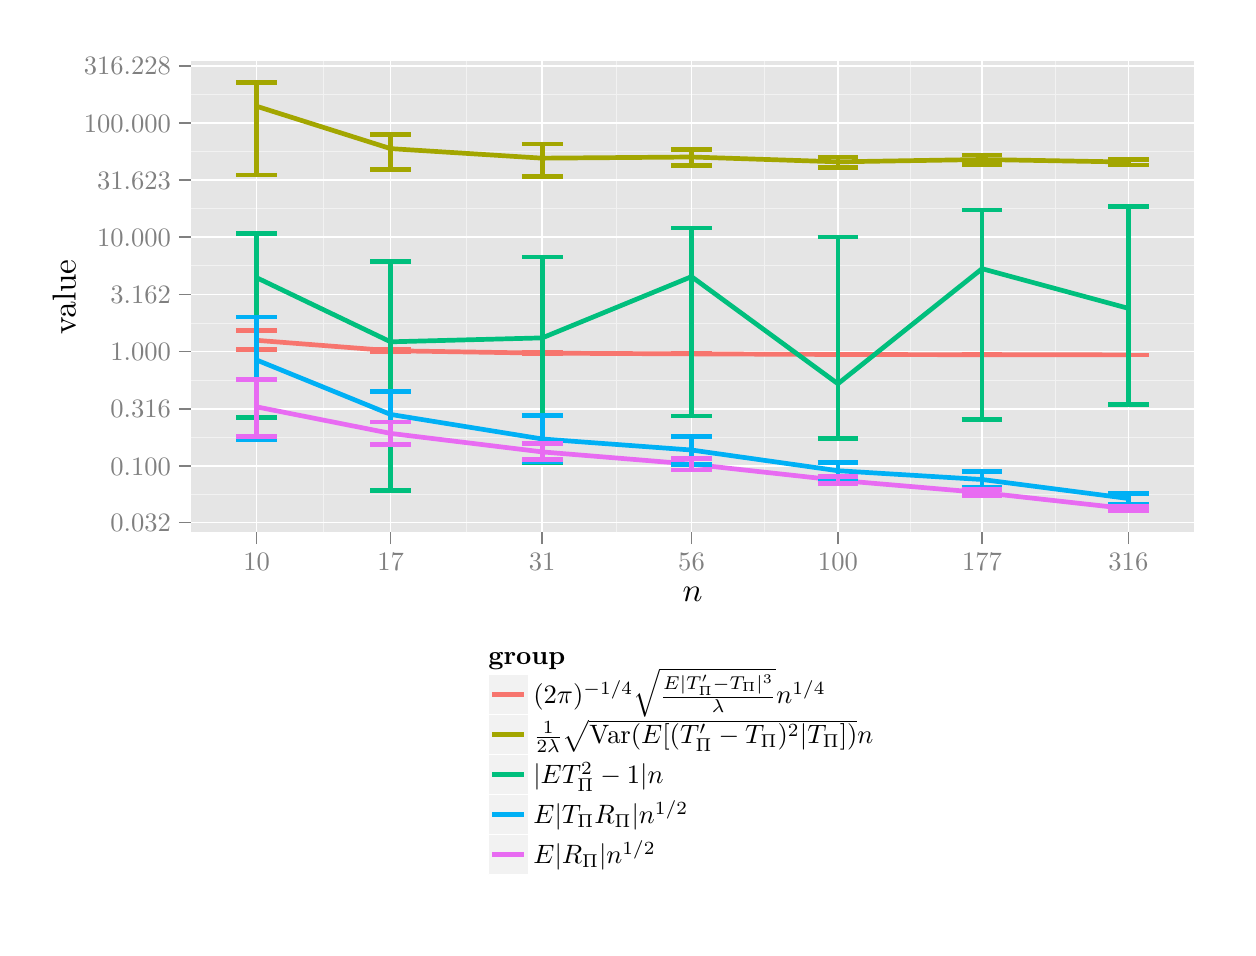
\begin{tikzpicture}[x=1pt,y=1pt]
\definecolor[named]{fillColor}{rgb}{1.00,1.00,1.00}
\path[use as bounding box,fill=fillColor,fill opacity=0.00] (0,0) rectangle (433.62,325.21);
\begin{scope}
\path[clip] (  0.00,  0.00) rectangle (433.62,325.21);
\definecolor[named]{drawColor}{rgb}{1.00,1.00,1.00}
\definecolor[named]{fillColor}{rgb}{1.00,1.00,1.00}

\path[draw=drawColor,line width= 0.6pt,line join=round,line cap=round,fill=fillColor] (  0.00,  0.00) rectangle (433.62,325.21);
\end{scope}
\begin{scope}
\path[clip] ( 58.88,142.81) rectangle (421.57,313.17);
\definecolor[named]{fillColor}{rgb}{0.90,0.90,0.90}

\path[fill=fillColor] ( 58.88,142.81) rectangle (421.57,313.17);
\definecolor[named]{drawColor}{rgb}{0.95,0.95,0.95}

\path[draw=drawColor,line width= 0.3pt,line join=round] ( 58.88,156.64) --
	(421.57,156.64);

\path[draw=drawColor,line width= 0.3pt,line join=round] ( 58.88,177.18) --
	(421.57,177.18);

\path[draw=drawColor,line width= 0.3pt,line join=round] ( 58.88,197.84) --
	(421.57,197.84);

\path[draw=drawColor,line width= 0.3pt,line join=round] ( 58.88,218.50) --
	(421.57,218.50);

\path[draw=drawColor,line width= 0.3pt,line join=round] ( 58.88,239.15) --
	(421.57,239.15);

\path[draw=drawColor,line width= 0.3pt,line join=round] ( 58.88,259.81) --
	(421.57,259.81);

\path[draw=drawColor,line width= 0.3pt,line join=round] ( 58.88,280.46) --
	(421.57,280.46);

\path[draw=drawColor,line width= 0.3pt,line join=round] ( 58.88,301.12) --
	(421.57,301.12);

\path[draw=drawColor,line width= 0.3pt,line join=round] (106.92,142.81) --
	(106.92,313.17);

\path[draw=drawColor,line width= 0.3pt,line join=round] (158.53,142.81) --
	(158.53,313.17);

\path[draw=drawColor,line width= 0.3pt,line join=round] (212.91,142.81) --
	(212.91,313.17);

\path[draw=drawColor,line width= 0.3pt,line join=round] (266.33,142.81) --
	(266.33,313.17);

\path[draw=drawColor,line width= 0.3pt,line join=round] (318.82,142.81) --
	(318.82,313.17);

\path[draw=drawColor,line width= 0.3pt,line join=round] (371.30,142.81) --
	(371.30,313.17);
\definecolor[named]{drawColor}{rgb}{1.00,1.00,1.00}

\path[draw=drawColor,line width= 0.6pt,line join=round] ( 58.88,146.42) --
	(421.57,146.42);

\path[draw=drawColor,line width= 0.6pt,line join=round] ( 58.88,166.86) --
	(421.57,166.86);

\path[draw=drawColor,line width= 0.6pt,line join=round] ( 58.88,187.50) --
	(421.57,187.50);

\path[draw=drawColor,line width= 0.6pt,line join=round] ( 58.88,208.17) --
	(421.57,208.17);

\path[draw=drawColor,line width= 0.6pt,line join=round] ( 58.88,228.82) --
	(421.57,228.82);

\path[draw=drawColor,line width= 0.6pt,line join=round] ( 58.88,249.48) --
	(421.57,249.48);

\path[draw=drawColor,line width= 0.6pt,line join=round] ( 58.88,270.13) --
	(421.57,270.13);

\path[draw=drawColor,line width= 0.6pt,line join=round] ( 58.88,290.79) --
	(421.57,290.79);

\path[draw=drawColor,line width= 0.6pt,line join=round] ( 58.88,311.44) --
	(421.57,311.44);

\path[draw=drawColor,line width= 0.6pt,line join=round] ( 82.72,142.81) --
	( 82.72,313.17);

\path[draw=drawColor,line width= 0.6pt,line join=round] (131.13,142.81) --
	(131.13,313.17);

\path[draw=drawColor,line width= 0.6pt,line join=round] (185.93,142.81) --
	(185.93,313.17);

\path[draw=drawColor,line width= 0.6pt,line join=round] (239.88,142.81) --
	(239.88,313.17);

\path[draw=drawColor,line width= 0.6pt,line join=round] (292.78,142.81) --
	(292.78,313.17);

\path[draw=drawColor,line width= 0.6pt,line join=round] (344.86,142.81) --
	(344.86,313.17);

\path[draw=drawColor,line width= 0.6pt,line join=round] (397.74,142.81) --
	(397.74,313.17);
\definecolor[named]{drawColor}{rgb}{0.97,0.46,0.43}

\path[draw=drawColor,line width= 1.7pt,line join=round] ( 82.72,212.23) --
	(131.13,208.47) --
	(185.93,207.59) --
	(239.88,207.33) --
	(292.78,207.11) --
	(344.86,207.03) --
	(397.74,206.97);
\definecolor[named]{drawColor}{rgb}{0.64,0.65,0.00}

\path[draw=drawColor,line width= 1.7pt,line join=round] ( 82.72,296.81) --
	(131.13,281.50) --
	(185.93,278.05) --
	(239.88,278.47) --
	(292.78,276.73) --
	(344.86,277.57) --
	(397.74,276.65);
\definecolor[named]{drawColor}{rgb}{0.00,0.75,0.49}

\path[draw=drawColor,line width= 1.7pt,line join=round] ( 82.72,234.87) --
	(131.13,211.69) --
	(185.93,213.11) --
	(239.88,235.24) --
	(292.78,196.53) --
	(344.86,238.11) --
	(397.74,223.78);
\definecolor[named]{drawColor}{rgb}{0.00,0.69,0.96}

\path[draw=drawColor,line width= 1.7pt,line join=round] ( 82.72,205.12) --
	(131.13,185.45) --
	(185.93,176.58) --
	(239.88,172.59) --
	(292.78,165.11) --
	(344.86,161.94) --
	(397.74,155.08);
\definecolor[named]{drawColor}{rgb}{0.91,0.42,0.95}

\path[draw=drawColor,line width= 1.7pt,line join=round] ( 82.72,188.19) --
	(131.13,178.60) --
	(185.93,171.91) --
	(239.88,167.48) --
	(292.78,161.66) --
	(344.86,157.21) --
	(397.74,151.36);
\definecolor[named]{drawColor}{rgb}{0.97,0.46,0.43}

\path[draw=drawColor,line width= 1.7pt,line join=round] ( 75.37,215.79) --
	( 90.07,215.79);

\path[draw=drawColor,line width= 1.7pt,line join=round] ( 82.72,215.79) --
	( 82.72,209.03);

\path[draw=drawColor,line width= 1.7pt,line join=round] ( 75.37,209.03) --
	( 90.07,209.03);

\path[draw=drawColor,line width= 1.7pt,line join=round] (123.78,209.01) --
	(138.48,209.01);

\path[draw=drawColor,line width= 1.7pt,line join=round] (131.13,209.01) --
	(131.13,207.96);

\path[draw=drawColor,line width= 1.7pt,line join=round] (123.78,207.96) --
	(138.48,207.96);

\path[draw=drawColor,line width= 1.7pt,line join=round] (178.58,207.78) --
	(193.28,207.78);

\path[draw=drawColor,line width= 1.7pt,line join=round] (185.93,207.78) --
	(185.93,207.43);

\path[draw=drawColor,line width= 1.7pt,line join=round] (178.58,207.43) --
	(193.28,207.43);

\path[draw=drawColor,line width= 1.7pt,line join=round] (232.53,207.40) --
	(247.23,207.40);

\path[draw=drawColor,line width= 1.7pt,line join=round] (239.88,207.40) --
	(239.88,207.26);

\path[draw=drawColor,line width= 1.7pt,line join=round] (232.53,207.26) --
	(247.23,207.26);

\path[draw=drawColor,line width= 1.7pt,line join=round] (285.42,207.14) --
	(300.13,207.14);

\path[draw=drawColor,line width= 1.7pt,line join=round] (292.78,207.14) --
	(292.78,207.09);

\path[draw=drawColor,line width= 1.7pt,line join=round] (285.42,207.09) --
	(300.13,207.09);

\path[draw=drawColor,line width= 1.7pt,line join=round] (337.51,207.04) --
	(352.22,207.04);

\path[draw=drawColor,line width= 1.7pt,line join=round] (344.86,207.04) --
	(344.86,207.01);

\path[draw=drawColor,line width= 1.7pt,line join=round] (337.51,207.01) --
	(352.22,207.01);

\path[draw=drawColor,line width= 1.7pt,line join=round] (390.39,206.98) --
	(405.09,206.98);

\path[draw=drawColor,line width= 1.7pt,line join=round] (397.74,206.98) --
	(397.74,206.97);

\path[draw=drawColor,line width= 1.7pt,line join=round] (390.39,206.97) --
	(405.09,206.97);
\definecolor[named]{drawColor}{rgb}{0.64,0.65,0.00}

\path[draw=drawColor,line width= 1.7pt,line join=round] ( 75.37,305.43) --
	( 90.07,305.43);

\path[draw=drawColor,line width= 1.7pt,line join=round] ( 82.72,305.43) --
	( 82.72,272.00);

\path[draw=drawColor,line width= 1.7pt,line join=round] ( 75.37,272.00) --
	( 90.07,272.00);

\path[draw=drawColor,line width= 1.7pt,line join=round] (123.78,286.57) --
	(138.48,286.57);

\path[draw=drawColor,line width= 1.7pt,line join=round] (131.13,286.57) --
	(131.13,273.88);

\path[draw=drawColor,line width= 1.7pt,line join=round] (123.78,273.88) --
	(138.48,273.88);

\path[draw=drawColor,line width= 1.7pt,line join=round] (178.58,283.20) --
	(193.28,283.20);

\path[draw=drawColor,line width= 1.7pt,line join=round] (185.93,283.20) --
	(185.93,271.44);

\path[draw=drawColor,line width= 1.7pt,line join=round] (178.58,271.44) --
	(193.28,271.44);

\path[draw=drawColor,line width= 1.7pt,line join=round] (232.53,281.15) --
	(247.23,281.15);

\path[draw=drawColor,line width= 1.7pt,line join=round] (239.88,281.15) --
	(239.88,275.41);

\path[draw=drawColor,line width= 1.7pt,line join=round] (232.53,275.41) --
	(247.23,275.41);

\path[draw=drawColor,line width= 1.7pt,line join=round] (285.42,278.48) --
	(300.13,278.48);

\path[draw=drawColor,line width= 1.7pt,line join=round] (292.78,278.48) --
	(292.78,274.78);

\path[draw=drawColor,line width= 1.7pt,line join=round] (285.42,274.78) --
	(300.13,274.78);

\path[draw=drawColor,line width= 1.7pt,line join=round] (337.51,279.20) --
	(352.22,279.20);

\path[draw=drawColor,line width= 1.7pt,line join=round] (344.86,279.20) --
	(344.86,275.70);

\path[draw=drawColor,line width= 1.7pt,line join=round] (337.51,275.70) --
	(352.22,275.70);

\path[draw=drawColor,line width= 1.7pt,line join=round] (390.39,277.66) --
	(405.09,277.66);

\path[draw=drawColor,line width= 1.7pt,line join=round] (397.74,277.66) --
	(397.74,275.55);

\path[draw=drawColor,line width= 1.7pt,line join=round] (390.39,275.55) --
	(405.09,275.55);
\definecolor[named]{drawColor}{rgb}{0.00,0.75,0.49}

\path[draw=drawColor,line width= 1.7pt,line join=round] ( 75.37,250.71) --
	( 90.07,250.71);

\path[draw=drawColor,line width= 1.7pt,line join=round] ( 82.72,250.71) --
	( 82.72,184.35);

\path[draw=drawColor,line width= 1.7pt,line join=round] ( 75.37,184.35) --
	( 90.07,184.35);

\path[draw=drawColor,line width= 1.7pt,line join=round] (123.78,240.65) --
	(138.48,240.65);

\path[draw=drawColor,line width= 1.7pt,line join=round] (131.13,240.65) --
	(131.13,157.85);

\path[draw=drawColor,line width= 1.7pt,line join=round] (123.78,157.85) --
	(138.48,157.85);

\path[draw=drawColor,line width= 1.7pt,line join=round] (178.58,242.36) --
	(193.28,242.36);

\path[draw=drawColor,line width= 1.7pt,line join=round] (185.93,242.36) --
	(185.93,168.02);

\path[draw=drawColor,line width= 1.7pt,line join=round] (178.58,168.02) --
	(193.28,168.02);

\path[draw=drawColor,line width= 1.7pt,line join=round] (232.53,252.82) --
	(247.23,252.82);

\path[draw=drawColor,line width= 1.7pt,line join=round] (239.88,252.82) --
	(239.88,184.90);

\path[draw=drawColor,line width= 1.7pt,line join=round] (232.53,184.90) --
	(247.23,184.90);

\path[draw=drawColor,line width= 1.7pt,line join=round] (285.42,249.54) --
	(300.13,249.54);

\path[draw=drawColor,line width= 1.7pt,line join=round] (292.78,249.54) --
	(292.78,176.72);

\path[draw=drawColor,line width= 1.7pt,line join=round] (285.42,176.72) --
	(300.13,176.72);

\path[draw=drawColor,line width= 1.7pt,line join=round] (337.51,259.28) --
	(352.22,259.28);

\path[draw=drawColor,line width= 1.7pt,line join=round] (344.86,259.28) --
	(344.86,183.59);

\path[draw=drawColor,line width= 1.7pt,line join=round] (337.51,183.59) --
	(352.22,183.59);

\path[draw=drawColor,line width= 1.7pt,line join=round] (390.39,260.67) --
	(405.09,260.67);

\path[draw=drawColor,line width= 1.7pt,line join=round] (397.74,260.67) --
	(397.74,189.01);

\path[draw=drawColor,line width= 1.7pt,line join=round] (390.39,189.01) --
	(405.09,189.01);
\definecolor[named]{drawColor}{rgb}{0.00,0.69,0.96}

\path[draw=drawColor,line width= 1.7pt,line join=round] ( 75.37,220.63) --
	( 90.07,220.63);

\path[draw=drawColor,line width= 1.7pt,line join=round] ( 82.72,220.63) --
	( 82.72,176.45);

\path[draw=drawColor,line width= 1.7pt,line join=round] ( 75.37,176.45) --
	( 90.07,176.45);

\path[draw=drawColor,line width= 1.7pt,line join=round] (123.78,193.86) --
	(138.48,193.86);

\path[draw=drawColor,line width= 1.7pt,line join=round] (131.13,193.86) --
	(131.13,174.67);

\path[draw=drawColor,line width= 1.7pt,line join=round] (123.78,174.67) --
	(138.48,174.67);

\path[draw=drawColor,line width= 1.7pt,line join=round] (178.58,185.02) --
	(193.28,185.02);

\path[draw=drawColor,line width= 1.7pt,line join=round] (185.93,185.02) --
	(185.93,168.34);

\path[draw=drawColor,line width= 1.7pt,line join=round] (178.58,168.34) --
	(193.28,168.34);

\path[draw=drawColor,line width= 1.7pt,line join=round] (232.53,177.45) --
	(247.23,177.45);

\path[draw=drawColor,line width= 1.7pt,line join=round] (239.88,177.45) --
	(239.88,167.34);

\path[draw=drawColor,line width= 1.7pt,line join=round] (232.53,167.34) --
	(247.23,167.34);

\path[draw=drawColor,line width= 1.7pt,line join=round] (285.42,168.13) --
	(300.13,168.13);

\path[draw=drawColor,line width= 1.7pt,line join=round] (292.78,168.13) --
	(292.78,161.90);

\path[draw=drawColor,line width= 1.7pt,line join=round] (285.42,161.90) --
	(300.13,161.90);

\path[draw=drawColor,line width= 1.7pt,line join=round] (337.51,164.95) --
	(352.22,164.95);

\path[draw=drawColor,line width= 1.7pt,line join=round] (344.86,164.95) --
	(344.86,158.98);

\path[draw=drawColor,line width= 1.7pt,line join=round] (337.51,158.98) --
	(352.22,158.98);

\path[draw=drawColor,line width= 1.7pt,line join=round] (390.39,156.99) --
	(405.09,156.99);

\path[draw=drawColor,line width= 1.7pt,line join=round] (397.74,156.99) --
	(397.74,153.12);

\path[draw=drawColor,line width= 1.7pt,line join=round] (390.39,153.12) --
	(405.09,153.12);
\definecolor[named]{drawColor}{rgb}{0.91,0.42,0.95}

\path[draw=drawColor,line width= 1.7pt,line join=round] ( 75.37,198.11) --
	( 90.07,198.11);

\path[draw=drawColor,line width= 1.7pt,line join=round] ( 82.72,198.11) --
	( 82.72,177.60);

\path[draw=drawColor,line width= 1.7pt,line join=round] ( 75.37,177.60) --
	( 90.07,177.60);

\path[draw=drawColor,line width= 1.7pt,line join=round] (123.78,182.73) --
	(138.48,182.73);

\path[draw=drawColor,line width= 1.7pt,line join=round] (131.13,182.73) --
	(131.13,174.52);

\path[draw=drawColor,line width= 1.7pt,line join=round] (123.78,174.52) --
	(138.48,174.52);

\path[draw=drawColor,line width= 1.7pt,line join=round] (178.58,175.06) --
	(193.28,175.06);

\path[draw=drawColor,line width= 1.7pt,line join=round] (185.93,175.06) --
	(185.93,169.10);

\path[draw=drawColor,line width= 1.7pt,line join=round] (178.58,169.10) --
	(193.28,169.10);

\path[draw=drawColor,line width= 1.7pt,line join=round] (232.53,169.53) --
	(247.23,169.53);

\path[draw=drawColor,line width= 1.7pt,line join=round] (239.88,169.53) --
	(239.88,165.42);

\path[draw=drawColor,line width= 1.7pt,line join=round] (232.53,165.42) --
	(247.23,165.42);

\path[draw=drawColor,line width= 1.7pt,line join=round] (285.42,162.96) --
	(300.13,162.96);

\path[draw=drawColor,line width= 1.7pt,line join=round] (292.78,162.96) --
	(292.78,160.37);

\path[draw=drawColor,line width= 1.7pt,line join=round] (285.42,160.37) --
	(300.13,160.37);

\path[draw=drawColor,line width= 1.7pt,line join=round] (337.51,158.45) --
	(352.22,158.45);

\path[draw=drawColor,line width= 1.7pt,line join=round] (344.86,158.45) --
	(344.86,156.04);

\path[draw=drawColor,line width= 1.7pt,line join=round] (337.51,156.04) --
	(352.22,156.04);

\path[draw=drawColor,line width= 1.7pt,line join=round] (390.39,152.16) --
	(405.09,152.16);

\path[draw=drawColor,line width= 1.7pt,line join=round] (397.74,152.16) --
	(397.74,150.56);

\path[draw=drawColor,line width= 1.7pt,line join=round] (390.39,150.56) --
	(405.09,150.56);
\end{scope}
\begin{scope}
\path[clip] (  0.00,  0.00) rectangle (433.62,325.21);
\definecolor[named]{drawColor}{rgb}{0.50,0.50,0.50}

\node[text=drawColor,anchor=base east,inner sep=0pt, outer sep=0pt, scale=  0.96] at ( 51.77,143.11) {0.032};

\node[text=drawColor,anchor=base east,inner sep=0pt, outer sep=0pt, scale=  0.96] at ( 51.77,163.55) {0.100};

\node[text=drawColor,anchor=base east,inner sep=0pt, outer sep=0pt, scale=  0.96] at ( 51.77,184.20) {0.316};

\node[text=drawColor,anchor=base east,inner sep=0pt, outer sep=0pt, scale=  0.96] at ( 51.77,204.86) {1.000};

\node[text=drawColor,anchor=base east,inner sep=0pt, outer sep=0pt, scale=  0.96] at ( 51.77,225.52) {3.162};

\node[text=drawColor,anchor=base east,inner sep=0pt, outer sep=0pt, scale=  0.96] at ( 51.77,246.17) {10.000};

\node[text=drawColor,anchor=base east,inner sep=0pt, outer sep=0pt, scale=  0.96] at ( 51.77,266.83) {31.623};

\node[text=drawColor,anchor=base east,inner sep=0pt, outer sep=0pt, scale=  0.96] at ( 51.77,287.48) {100.000};

\node[text=drawColor,anchor=base east,inner sep=0pt, outer sep=0pt, scale=  0.96] at ( 51.77,308.14) {316.228};
\end{scope}
\begin{scope}
\path[clip] (  0.00,  0.00) rectangle (433.62,325.21);
\definecolor[named]{drawColor}{rgb}{0.50,0.50,0.50}

\path[draw=drawColor,line width= 0.6pt,line join=round] ( 54.61,146.42) --
	( 58.88,146.42);

\path[draw=drawColor,line width= 0.6pt,line join=round] ( 54.61,166.86) --
	( 58.88,166.86);

\path[draw=drawColor,line width= 0.6pt,line join=round] ( 54.61,187.50) --
	( 58.88,187.50);

\path[draw=drawColor,line width= 0.6pt,line join=round] ( 54.61,208.17) --
	( 58.88,208.17);

\path[draw=drawColor,line width= 0.6pt,line join=round] ( 54.61,228.82) --
	( 58.88,228.82);

\path[draw=drawColor,line width= 0.6pt,line join=round] ( 54.61,249.48) --
	( 58.88,249.48);

\path[draw=drawColor,line width= 0.6pt,line join=round] ( 54.61,270.13) --
	( 58.88,270.13);

\path[draw=drawColor,line width= 0.6pt,line join=round] ( 54.61,290.79) --
	( 58.88,290.79);

\path[draw=drawColor,line width= 0.6pt,line join=round] ( 54.61,311.44) --
	( 58.88,311.44);
\end{scope}
\begin{scope}
\path[clip] (  0.00,  0.00) rectangle (433.62,325.21);
\definecolor[named]{drawColor}{rgb}{0.50,0.50,0.50}

\path[draw=drawColor,line width= 0.6pt,line join=round] ( 82.72,138.55) --
	( 82.72,142.81);

\path[draw=drawColor,line width= 0.6pt,line join=round] (131.13,138.55) --
	(131.13,142.81);

\path[draw=drawColor,line width= 0.6pt,line join=round] (185.93,138.55) --
	(185.93,142.81);

\path[draw=drawColor,line width= 0.6pt,line join=round] (239.88,138.55) --
	(239.88,142.81);

\path[draw=drawColor,line width= 0.6pt,line join=round] (292.78,138.55) --
	(292.78,142.81);

\path[draw=drawColor,line width= 0.6pt,line join=round] (344.86,138.55) --
	(344.86,142.81);

\path[draw=drawColor,line width= 0.6pt,line join=round] (397.74,138.55) --
	(397.74,142.81);
\end{scope}
\begin{scope}
\path[clip] (  0.00,  0.00) rectangle (433.62,325.21);
\definecolor[named]{drawColor}{rgb}{0.50,0.50,0.50}

\node[text=drawColor,anchor=base,inner sep=0pt, outer sep=0pt, scale=  0.96] at ( 82.72,129.09) {10};

\node[text=drawColor,anchor=base,inner sep=0pt, outer sep=0pt, scale=  0.96] at (131.13,129.09) {17};

\node[text=drawColor,anchor=base,inner sep=0pt, outer sep=0pt, scale=  0.96] at (185.93,129.09) {31};

\node[text=drawColor,anchor=base,inner sep=0pt, outer sep=0pt, scale=  0.96] at (239.88,129.09) {56};

\node[text=drawColor,anchor=base,inner sep=0pt, outer sep=0pt, scale=  0.96] at (292.78,129.09) {100};

\node[text=drawColor,anchor=base,inner sep=0pt, outer sep=0pt, scale=  0.96] at (344.86,129.09) {177};

\node[text=drawColor,anchor=base,inner sep=0pt, outer sep=0pt, scale=  0.96] at (397.74,129.09) {316};
\end{scope}
\begin{scope}
\path[clip] (  0.00,  0.00) rectangle (433.62,325.21);
\definecolor[named]{drawColor}{rgb}{0.00,0.00,0.00}

\node[text=drawColor,anchor=base,inner sep=0pt, outer sep=0pt, scale=  1.20] at (240.23,117.81) {$n$};
\end{scope}
\begin{scope}
\path[clip] (  0.00,  0.00) rectangle (433.62,325.21);
\definecolor[named]{drawColor}{rgb}{0.00,0.00,0.00}

\node[text=drawColor,rotate= 90.00,anchor=base,inner sep=0pt, outer sep=0pt, scale=  1.20] at ( 17.30,227.99) {value};
\end{scope}
\begin{scope}
\path[clip] (  0.00,  0.00) rectangle (433.62,325.21);
\definecolor[named]{fillColor}{rgb}{1.00,1.00,1.00}

\path[fill=fillColor] (162.21, 14.89) rectangle (318.25,105.93);
\end{scope}
\begin{scope}
\path[clip] (  0.00,  0.00) rectangle (433.62,325.21);
\definecolor[named]{drawColor}{rgb}{0.00,0.00,0.00}

\node[text=drawColor,anchor=base west,inner sep=0pt, outer sep=0pt, scale=  0.96] at (166.47, 95.04) {\bfseries group};
\end{scope}
\begin{scope}
\path[clip] (  0.00,  0.00) rectangle (433.62,325.21);
\definecolor[named]{drawColor}{rgb}{1.00,1.00,1.00}
\definecolor[named]{fillColor}{rgb}{0.95,0.95,0.95}

\path[draw=drawColor,line width= 0.6pt,line join=round,line cap=round,fill=fillColor] (166.47, 76.97) rectangle (180.93, 91.43);
\end{scope}
\begin{scope}
\path[clip] (  0.00,  0.00) rectangle (433.62,325.21);
\definecolor[named]{drawColor}{rgb}{0.97,0.46,0.43}

\path[draw=drawColor,line width= 1.7pt,line join=round] (167.92, 84.20) -- (179.48, 84.20);
\end{scope}
\begin{scope}
\path[clip] (  0.00,  0.00) rectangle (433.62,325.21);
\definecolor[named]{drawColor}{rgb}{0.97,0.46,0.43}

\path[draw=drawColor,line width= 1.7pt,line join=round] (167.92, 84.20) -- (179.48, 84.20);
\end{scope}
\begin{scope}
\path[clip] (  0.00,  0.00) rectangle (433.62,325.21);
\definecolor[named]{drawColor}{rgb}{1.00,1.00,1.00}
\definecolor[named]{fillColor}{rgb}{0.95,0.95,0.95}

\path[draw=drawColor,line width= 0.6pt,line join=round,line cap=round,fill=fillColor] (166.47, 62.52) rectangle (180.93, 76.97);
\end{scope}
\begin{scope}
\path[clip] (  0.00,  0.00) rectangle (433.62,325.21);
\definecolor[named]{drawColor}{rgb}{0.64,0.65,0.00}

\path[draw=drawColor,line width= 1.7pt,line join=round] (167.92, 69.75) -- (179.48, 69.75);
\end{scope}
\begin{scope}
\path[clip] (  0.00,  0.00) rectangle (433.62,325.21);
\definecolor[named]{drawColor}{rgb}{0.64,0.65,0.00}

\path[draw=drawColor,line width= 1.7pt,line join=round] (167.92, 69.75) -- (179.48, 69.75);
\end{scope}
\begin{scope}
\path[clip] (  0.00,  0.00) rectangle (433.62,325.21);
\definecolor[named]{drawColor}{rgb}{1.00,1.00,1.00}
\definecolor[named]{fillColor}{rgb}{0.95,0.95,0.95}

\path[draw=drawColor,line width= 0.6pt,line join=round,line cap=round,fill=fillColor] (166.47, 48.07) rectangle (180.93, 62.52);
\end{scope}
\begin{scope}
\path[clip] (  0.00,  0.00) rectangle (433.62,325.21);
\definecolor[named]{drawColor}{rgb}{0.00,0.75,0.49}

\path[draw=drawColor,line width= 1.7pt,line join=round] (167.92, 55.29) -- (179.48, 55.29);
\end{scope}
\begin{scope}
\path[clip] (  0.00,  0.00) rectangle (433.62,325.21);
\definecolor[named]{drawColor}{rgb}{0.00,0.75,0.49}

\path[draw=drawColor,line width= 1.7pt,line join=round] (167.92, 55.29) -- (179.48, 55.29);
\end{scope}
\begin{scope}
\path[clip] (  0.00,  0.00) rectangle (433.62,325.21);
\definecolor[named]{drawColor}{rgb}{1.00,1.00,1.00}
\definecolor[named]{fillColor}{rgb}{0.95,0.95,0.95}

\path[draw=drawColor,line width= 0.6pt,line join=round,line cap=round,fill=fillColor] (166.47, 33.61) rectangle (180.93, 48.07);
\end{scope}
\begin{scope}
\path[clip] (  0.00,  0.00) rectangle (433.62,325.21);
\definecolor[named]{drawColor}{rgb}{0.00,0.69,0.96}

\path[draw=drawColor,line width= 1.7pt,line join=round] (167.92, 40.84) -- (179.48, 40.84);
\end{scope}
\begin{scope}
\path[clip] (  0.00,  0.00) rectangle (433.62,325.21);
\definecolor[named]{drawColor}{rgb}{0.00,0.69,0.96}

\path[draw=drawColor,line width= 1.7pt,line join=round] (167.92, 40.84) -- (179.48, 40.84);
\end{scope}
\begin{scope}
\path[clip] (  0.00,  0.00) rectangle (433.62,325.21);
\definecolor[named]{drawColor}{rgb}{1.00,1.00,1.00}
\definecolor[named]{fillColor}{rgb}{0.95,0.95,0.95}

\path[draw=drawColor,line width= 0.6pt,line join=round,line cap=round,fill=fillColor] (166.47, 19.16) rectangle (180.93, 33.61);
\end{scope}
\begin{scope}
\path[clip] (  0.00,  0.00) rectangle (433.62,325.21);
\definecolor[named]{drawColor}{rgb}{0.91,0.42,0.95}

\path[draw=drawColor,line width= 1.7pt,line join=round] (167.92, 26.39) -- (179.48, 26.39);
\end{scope}
\begin{scope}
\path[clip] (  0.00,  0.00) rectangle (433.62,325.21);
\definecolor[named]{drawColor}{rgb}{0.91,0.42,0.95}

\path[draw=drawColor,line width= 1.7pt,line join=round] (167.92, 26.39) -- (179.48, 26.39);
\end{scope}
\begin{scope}
\path[clip] (  0.00,  0.00) rectangle (433.62,325.21);
\definecolor[named]{drawColor}{rgb}{0.00,0.00,0.00}

\node[text=drawColor,anchor=base west,inner sep=0pt, outer sep=0pt, scale=  0.96] at (182.73, 80.90) {$(2\pi)^{-1/4}\sqrt{\frac{\mathbb{E}|T'_{\Pi}-T_{\Pi}|^3}{\lambda}}n^{1/4}\quad $};
\end{scope}
\begin{scope}
\path[clip] (  0.00,  0.00) rectangle (433.62,325.21);
\definecolor[named]{drawColor}{rgb}{0.00,0.00,0.00}

\node[text=drawColor,anchor=base west,inner sep=0pt, outer sep=0pt, scale=  0.96] at (182.73, 66.44) {$\frac{1}{2\lambda}\sqrt{\mathrm{Var}(\mathbb{E}[(T'_{\Pi}-T_{\Pi})^2|T_{\Pi}])}n\quad $};
\end{scope}
\begin{scope}
\path[clip] (  0.00,  0.00) rectangle (433.62,325.21);
\definecolor[named]{drawColor}{rgb}{0.00,0.00,0.00}

\node[text=drawColor,anchor=base west,inner sep=0pt, outer sep=0pt, scale=  0.96] at (182.73, 51.99) {$|\mathbb{E}T_{\Pi}^2-1|n\quad $};
\end{scope}
\begin{scope}
\path[clip] (  0.00,  0.00) rectangle (433.62,325.21);
\definecolor[named]{drawColor}{rgb}{0.00,0.00,0.00}

\node[text=drawColor,anchor=base west,inner sep=0pt, outer sep=0pt, scale=  0.96] at (182.73, 37.53) {$\mathbb{E}|T_{\Pi}R_{\Pi}|n^{1/2}\quad $};
\end{scope}
\begin{scope}
\path[clip] (  0.00,  0.00) rectangle (433.62,325.21);
\definecolor[named]{drawColor}{rgb}{0.00,0.00,0.00}

\node[text=drawColor,anchor=base west,inner sep=0pt, outer sep=0pt, scale=  0.96] at (182.73, 23.08) {$\mathbb{E}|R_{\Pi}|n^{1/2}\quad $};
\end{scope}
\end{tikzpicture}

    }
  \end{center}
\end{frame}

\begin{frame}{Simulated Bounds (Improved Rate)}
  \begin{center}
    \resizebox{9.0cm}{!}{
      % Created by tikzDevice version 0.6.2-92-0ad2792 on 2013-05-05 16:12:42
% !TEX encoding = UTF-8 Unicode
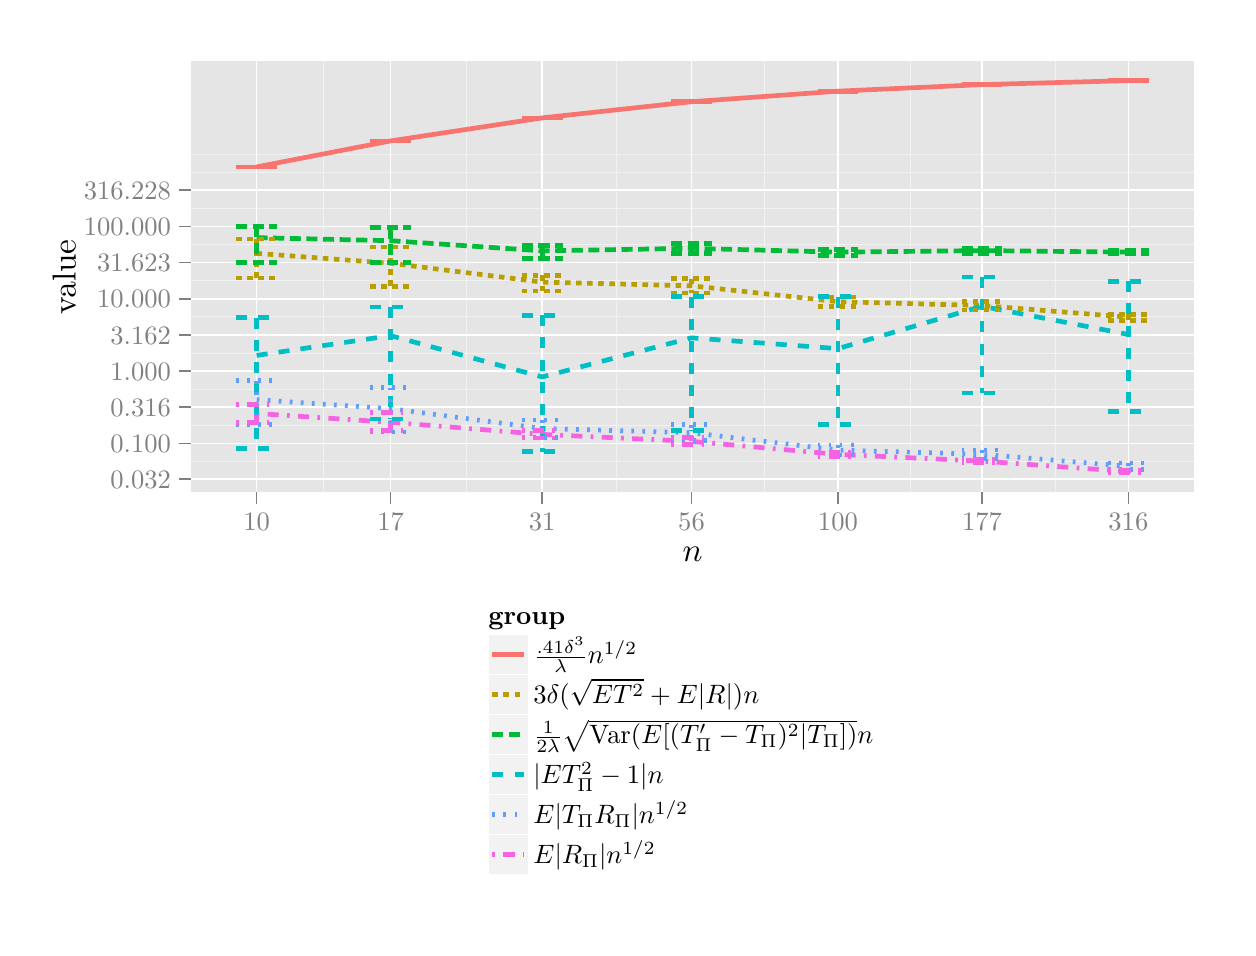
\begin{tikzpicture}[x=1pt,y=1pt]
\definecolor[named]{fillColor}{rgb}{1.00,1.00,1.00}
\path[use as bounding box,fill=fillColor,fill opacity=0.00] (0,0) rectangle (433.62,325.21);
\begin{scope}
\path[clip] (  0.00,  0.00) rectangle (433.62,325.21);
\definecolor[named]{drawColor}{rgb}{1.00,1.00,1.00}
\definecolor[named]{fillColor}{rgb}{1.00,1.00,1.00}

\path[draw=drawColor,line width= 0.6pt,line join=round,line cap=round,fill=fillColor] (  0.00,  0.00) rectangle (433.62,325.21);
\end{scope}
\begin{scope}
\path[clip] ( 58.88,157.27) rectangle (421.57,313.17);
\definecolor[named]{fillColor}{rgb}{0.90,0.90,0.90}

\path[fill=fillColor] ( 58.88,157.27) rectangle (421.57,313.17);
\definecolor[named]{drawColor}{rgb}{0.95,0.95,0.95}

\path[draw=drawColor,line width= 0.3pt,line join=round] ( 58.88,168.50) --
	(421.57,168.50);

\path[draw=drawColor,line width= 0.3pt,line join=round] ( 58.88,181.50) --
	(421.57,181.50);

\path[draw=drawColor,line width= 0.3pt,line join=round] ( 58.88,194.57) --
	(421.57,194.57);

\path[draw=drawColor,line width= 0.3pt,line join=round] ( 58.88,207.64) --
	(421.57,207.64);

\path[draw=drawColor,line width= 0.3pt,line join=round] ( 58.88,220.71) --
	(421.57,220.71);

\path[draw=drawColor,line width= 0.3pt,line join=round] ( 58.88,233.78) --
	(421.57,233.78);

\path[draw=drawColor,line width= 0.3pt,line join=round] ( 58.88,246.85) --
	(421.57,246.85);

\path[draw=drawColor,line width= 0.3pt,line join=round] ( 58.88,259.92) --
	(421.57,259.92);

\path[draw=drawColor,line width= 0.3pt,line join=round] ( 58.88,272.93) --
	(421.57,272.93);

\path[draw=drawColor,line width= 0.3pt,line join=round] ( 58.88,279.39) --
	(421.57,279.39);

\path[draw=drawColor,line width= 0.3pt,line join=round] (106.92,157.27) --
	(106.92,313.17);

\path[draw=drawColor,line width= 0.3pt,line join=round] (158.53,157.27) --
	(158.53,313.17);

\path[draw=drawColor,line width= 0.3pt,line join=round] (212.91,157.27) --
	(212.91,313.17);

\path[draw=drawColor,line width= 0.3pt,line join=round] (266.33,157.27) --
	(266.33,313.17);

\path[draw=drawColor,line width= 0.3pt,line join=round] (318.82,157.27) --
	(318.82,313.17);

\path[draw=drawColor,line width= 0.3pt,line join=round] (371.30,157.27) --
	(371.30,313.17);
\definecolor[named]{drawColor}{rgb}{1.00,1.00,1.00}

\path[draw=drawColor,line width= 0.6pt,line join=round] ( 58.88,162.03) --
	(421.57,162.03);

\path[draw=drawColor,line width= 0.6pt,line join=round] ( 58.88,174.97) --
	(421.57,174.97);

\path[draw=drawColor,line width= 0.6pt,line join=round] ( 58.88,188.03) --
	(421.57,188.03);

\path[draw=drawColor,line width= 0.6pt,line join=round] ( 58.88,201.11) --
	(421.57,201.11);

\path[draw=drawColor,line width= 0.6pt,line join=round] ( 58.88,214.18) --
	(421.57,214.18);

\path[draw=drawColor,line width= 0.6pt,line join=round] ( 58.88,227.25) --
	(421.57,227.25);

\path[draw=drawColor,line width= 0.6pt,line join=round] ( 58.88,240.32) --
	(421.57,240.32);

\path[draw=drawColor,line width= 0.6pt,line join=round] ( 58.88,253.39) --
	(421.57,253.39);

\path[draw=drawColor,line width= 0.6pt,line join=round] ( 58.88,266.46) --
	(421.57,266.46);

\path[draw=drawColor,line width= 0.6pt,line join=round] ( 82.72,157.27) --
	( 82.72,313.17);

\path[draw=drawColor,line width= 0.6pt,line join=round] (131.13,157.27) --
	(131.13,313.17);

\path[draw=drawColor,line width= 0.6pt,line join=round] (185.93,157.27) --
	(185.93,313.17);

\path[draw=drawColor,line width= 0.6pt,line join=round] (239.88,157.27) --
	(239.88,313.17);

\path[draw=drawColor,line width= 0.6pt,line join=round] (292.78,157.27) --
	(292.78,313.17);

\path[draw=drawColor,line width= 0.6pt,line join=round] (344.86,157.27) --
	(344.86,313.17);

\path[draw=drawColor,line width= 0.6pt,line join=round] (397.74,157.27) --
	(397.74,313.17);
\definecolor[named]{drawColor}{rgb}{0.97,0.46,0.43}

\path[draw=drawColor,line width= 1.7pt,line join=round] ( 82.72,274.89) --
	(131.13,284.28) --
	(185.93,292.61) --
	(239.88,298.45) --
	(292.78,302.26) --
	(344.86,304.63) --
	(397.74,306.08);
\definecolor[named]{drawColor}{rgb}{0.72,0.62,0.00}

\path[draw=drawColor,line width= 1.7pt,dash pattern=on 2pt off 2pt ,line join=round] ( 82.72,243.66) --
	(131.13,240.08) --
	(185.93,233.27) --
	(239.88,231.93) --
	(292.78,226.20) --
	(344.86,224.80) --
	(397.74,220.60);
\definecolor[named]{drawColor}{rgb}{0.00,0.73,0.22}

\path[draw=drawColor,line width= 1.7pt,dash pattern=on 4pt off 2pt ,line join=round] ( 82.72,249.33) --
	(131.13,248.23) --
	(185.93,244.56) --
	(239.88,245.48) --
	(292.78,244.09) --
	(344.86,244.65) --
	(397.74,244.10);
\definecolor[named]{drawColor}{rgb}{0.00,0.75,0.77}

\path[draw=drawColor,line width= 1.7pt,dash pattern=on 4pt off 4pt ,line join=round] ( 82.72,206.77) --
	(131.13,213.92) --
	(185.93,199.00) --
	(239.88,213.13) --
	(292.78,209.23) --
	(344.86,224.54) --
	(397.74,214.35);
\definecolor[named]{drawColor}{rgb}{0.38,0.61,1.00}

\path[draw=drawColor,line width= 1.7pt,dash pattern=on 1pt off 3pt ,line join=round] ( 82.72,190.78) --
	(131.13,187.54) --
	(185.93,180.37) --
	(239.88,178.84) --
	(292.78,172.56) --
	(344.86,171.06) --
	(397.74,166.69);
\definecolor[named]{drawColor}{rgb}{0.96,0.39,0.89}

\path[draw=drawColor,line width= 1.7pt,dash pattern=on 1pt off 3pt on 4pt off 3pt ,line join=round] ( 82.72,185.80) --
	(131.13,182.62) --
	(185.93,178.24) --
	(239.88,175.72) --
	(292.78,171.01) --
	(344.86,168.59) --
	(397.74,164.80);
\definecolor[named]{drawColor}{rgb}{0.97,0.46,0.43}

\path[draw=drawColor,line width= 1.7pt,line join=round] ( 75.37,274.89) --
	( 90.07,274.89);

\path[draw=drawColor,line width= 1.7pt,line join=round] ( 82.72,274.89) --
	( 82.72,274.89);

\path[draw=drawColor,line width= 1.7pt,line join=round] ( 75.37,274.89) --
	( 90.07,274.89);

\path[draw=drawColor,line width= 1.7pt,line join=round] (123.78,284.28) --
	(138.48,284.28);

\path[draw=drawColor,line width= 1.7pt,line join=round] (131.13,284.28) --
	(131.13,284.28);

\path[draw=drawColor,line width= 1.7pt,line join=round] (123.78,284.28) --
	(138.48,284.28);

\path[draw=drawColor,line width= 1.7pt,line join=round] (178.58,292.61) --
	(193.28,292.61);

\path[draw=drawColor,line width= 1.7pt,line join=round] (185.93,292.61) --
	(185.93,292.61);

\path[draw=drawColor,line width= 1.7pt,line join=round] (178.58,292.61) --
	(193.28,292.61);

\path[draw=drawColor,line width= 1.7pt,line join=round] (232.53,298.45) --
	(247.23,298.45);

\path[draw=drawColor,line width= 1.7pt,line join=round] (239.88,298.45) --
	(239.88,298.45);

\path[draw=drawColor,line width= 1.7pt,line join=round] (232.53,298.45) --
	(247.23,298.45);

\path[draw=drawColor,line width= 1.7pt,line join=round] (285.42,302.26) --
	(300.13,302.26);

\path[draw=drawColor,line width= 1.7pt,line join=round] (292.78,302.26) --
	(292.78,302.26);

\path[draw=drawColor,line width= 1.7pt,line join=round] (285.42,302.26) --
	(300.13,302.26);

\path[draw=drawColor,line width= 1.7pt,line join=round] (337.51,304.63) --
	(352.22,304.63);

\path[draw=drawColor,line width= 1.7pt,line join=round] (344.86,304.63) --
	(344.86,304.63);

\path[draw=drawColor,line width= 1.7pt,line join=round] (337.51,304.63) --
	(352.22,304.63);

\path[draw=drawColor,line width= 1.7pt,line join=round] (390.39,306.08) --
	(405.09,306.08);

\path[draw=drawColor,line width= 1.7pt,line join=round] (397.74,306.08) --
	(397.74,306.08);

\path[draw=drawColor,line width= 1.7pt,line join=round] (390.39,306.08) --
	(405.09,306.08);
\definecolor[named]{drawColor}{rgb}{0.72,0.62,0.00}

\path[draw=drawColor,line width= 1.7pt,dash pattern=on 2pt off 2pt ,line join=round] ( 75.37,248.87) --
	( 90.07,248.87);

\path[draw=drawColor,line width= 1.7pt,dash pattern=on 2pt off 2pt ,line join=round] ( 82.72,248.87) --
	( 82.72,234.74);

\path[draw=drawColor,line width= 1.7pt,dash pattern=on 2pt off 2pt ,line join=round] ( 75.37,234.74) --
	( 90.07,234.74);

\path[draw=drawColor,line width= 1.7pt,dash pattern=on 2pt off 2pt ,line join=round] (123.78,245.97) --
	(138.48,245.97);

\path[draw=drawColor,line width= 1.7pt,dash pattern=on 2pt off 2pt ,line join=round] (131.13,245.97) --
	(131.13,231.80);

\path[draw=drawColor,line width= 1.7pt,dash pattern=on 2pt off 2pt ,line join=round] (123.78,231.80) --
	(138.48,231.80);

\path[draw=drawColor,line width= 1.7pt,dash pattern=on 2pt off 2pt ,line join=round] (178.58,235.77) --
	(193.28,235.77);

\path[draw=drawColor,line width= 1.7pt,dash pattern=on 2pt off 2pt ,line join=round] (185.93,235.77) --
	(185.93,230.09);

\path[draw=drawColor,line width= 1.7pt,dash pattern=on 2pt off 2pt ,line join=round] (178.58,230.09) --
	(193.28,230.09);

\path[draw=drawColor,line width= 1.7pt,dash pattern=on 2pt off 2pt ,line join=round] (232.53,234.49) --
	(247.23,234.49);

\path[draw=drawColor,line width= 1.7pt,dash pattern=on 2pt off 2pt ,line join=round] (239.88,234.49) --
	(239.88,229.34);

\path[draw=drawColor,line width= 1.7pt,dash pattern=on 2pt off 2pt ,line join=round] (232.53,229.34) --
	(247.23,229.34);

\path[draw=drawColor,line width= 1.7pt,dash pattern=on 2pt off 2pt ,line join=round] (285.42,227.86) --
	(300.13,227.86);

\path[draw=drawColor,line width= 1.7pt,dash pattern=on 2pt off 2pt ,line join=round] (292.78,227.86) --
	(292.78,224.41);

\path[draw=drawColor,line width= 1.7pt,dash pattern=on 2pt off 2pt ,line join=round] (285.42,224.41) --
	(300.13,224.41);

\path[draw=drawColor,line width= 1.7pt,dash pattern=on 2pt off 2pt ,line join=round] (337.51,226.29) --
	(352.22,226.29);

\path[draw=drawColor,line width= 1.7pt,dash pattern=on 2pt off 2pt ,line join=round] (344.86,226.29) --
	(344.86,223.23);

\path[draw=drawColor,line width= 1.7pt,dash pattern=on 2pt off 2pt ,line join=round] (337.51,223.23) --
	(352.22,223.23);

\path[draw=drawColor,line width= 1.7pt,dash pattern=on 2pt off 2pt ,line join=round] (390.39,221.68) --
	(405.09,221.68);

\path[draw=drawColor,line width= 1.7pt,dash pattern=on 2pt off 2pt ,line join=round] (397.74,221.68) --
	(397.74,219.48);

\path[draw=drawColor,line width= 1.7pt,dash pattern=on 2pt off 2pt ,line join=round] (390.39,219.48) --
	(405.09,219.48);
\definecolor[named]{drawColor}{rgb}{0.00,0.73,0.22}

\path[draw=drawColor,line width= 1.7pt,dash pattern=on 4pt off 2pt ,line join=round] ( 75.37,253.42) --
	( 90.07,253.42);

\path[draw=drawColor,line width= 1.7pt,dash pattern=on 4pt off 2pt ,line join=round] ( 82.72,253.42) --
	( 82.72,240.31);

\path[draw=drawColor,line width= 1.7pt,dash pattern=on 4pt off 2pt ,line join=round] ( 75.37,240.31) --
	( 90.07,240.31);

\path[draw=drawColor,line width= 1.7pt,dash pattern=on 4pt off 2pt ,line join=round] (123.78,252.95) --
	(138.48,252.95);

\path[draw=drawColor,line width= 1.7pt,dash pattern=on 4pt off 2pt ,line join=round] (131.13,252.95) --
	(131.13,240.33);

\path[draw=drawColor,line width= 1.7pt,dash pattern=on 4pt off 2pt ,line join=round] (123.78,240.33) --
	(138.48,240.33);

\path[draw=drawColor,line width= 1.7pt,dash pattern=on 4pt off 2pt ,line join=round] (178.58,246.46) --
	(193.28,246.46);

\path[draw=drawColor,line width= 1.7pt,dash pattern=on 4pt off 2pt ,line join=round] (185.93,246.46) --
	(185.93,241.88);

\path[draw=drawColor,line width= 1.7pt,dash pattern=on 4pt off 2pt ,line join=round] (178.58,241.88) --
	(193.28,241.88);

\path[draw=drawColor,line width= 1.7pt,dash pattern=on 4pt off 2pt ,line join=round] (232.53,247.11) --
	(247.23,247.11);

\path[draw=drawColor,line width= 1.7pt,dash pattern=on 4pt off 2pt ,line join=round] (239.88,247.11) --
	(239.88,243.71);

\path[draw=drawColor,line width= 1.7pt,dash pattern=on 4pt off 2pt ,line join=round] (232.53,243.71) --
	(247.23,243.71);

\path[draw=drawColor,line width= 1.7pt,dash pattern=on 4pt off 2pt ,line join=round] (285.42,245.16) --
	(300.13,245.16);

\path[draw=drawColor,line width= 1.7pt,dash pattern=on 4pt off 2pt ,line join=round] (292.78,245.16) --
	(292.78,242.89);

\path[draw=drawColor,line width= 1.7pt,dash pattern=on 4pt off 2pt ,line join=round] (285.42,242.89) --
	(300.13,242.89);

\path[draw=drawColor,line width= 1.7pt,dash pattern=on 4pt off 2pt ,line join=round] (337.51,245.53) --
	(352.22,245.53);

\path[draw=drawColor,line width= 1.7pt,dash pattern=on 4pt off 2pt ,line join=round] (344.86,245.53) --
	(344.86,243.65);

\path[draw=drawColor,line width= 1.7pt,dash pattern=on 4pt off 2pt ,line join=round] (337.51,243.65) --
	(352.22,243.65);

\path[draw=drawColor,line width= 1.7pt,dash pattern=on 4pt off 2pt ,line join=round] (390.39,244.74) --
	(405.09,244.74);

\path[draw=drawColor,line width= 1.7pt,dash pattern=on 4pt off 2pt ,line join=round] (397.74,244.74) --
	(397.74,243.44);

\path[draw=drawColor,line width= 1.7pt,dash pattern=on 4pt off 2pt ,line join=round] (390.39,243.44) --
	(405.09,243.44);
\definecolor[named]{drawColor}{rgb}{0.00,0.75,0.77}

\path[draw=drawColor,line width= 1.7pt,dash pattern=on 4pt off 4pt ,line join=round] ( 75.37,220.42) --
	( 90.07,220.42);

\path[draw=drawColor,line width= 1.7pt,dash pattern=on 4pt off 4pt ,line join=round] ( 82.72,220.42) --
	( 82.72,173.09);

\path[draw=drawColor,line width= 1.7pt,dash pattern=on 4pt off 4pt ,line join=round] ( 75.37,173.09) --
	( 90.07,173.09);

\path[draw=drawColor,line width= 1.7pt,dash pattern=on 4pt off 4pt ,line join=round] (123.78,224.22) --
	(138.48,224.22);

\path[draw=drawColor,line width= 1.7pt,dash pattern=on 4pt off 4pt ,line join=round] (131.13,224.22) --
	(131.13,183.80);

\path[draw=drawColor,line width= 1.7pt,dash pattern=on 4pt off 4pt ,line join=round] (123.78,183.80) --
	(138.48,183.80);

\path[draw=drawColor,line width= 1.7pt,dash pattern=on 4pt off 4pt ,line join=round] (178.58,221.29) --
	(193.28,221.29);

\path[draw=drawColor,line width= 1.7pt,dash pattern=on 4pt off 4pt ,line join=round] (185.93,221.29) --
	(185.93,172.02);

\path[draw=drawColor,line width= 1.7pt,dash pattern=on 4pt off 4pt ,line join=round] (178.58,172.02) --
	(193.28,172.02);

\path[draw=drawColor,line width= 1.7pt,dash pattern=on 4pt off 4pt ,line join=round] (232.53,228.00) --
	(247.23,228.00);

\path[draw=drawColor,line width= 1.7pt,dash pattern=on 4pt off 4pt ,line join=round] (239.88,228.00) --
	(239.88,179.75);

\path[draw=drawColor,line width= 1.7pt,dash pattern=on 4pt off 4pt ,line join=round] (232.53,179.75) --
	(247.23,179.75);

\path[draw=drawColor,line width= 1.7pt,dash pattern=on 4pt off 4pt ,line join=round] (285.42,228.02) --
	(300.13,228.02);

\path[draw=drawColor,line width= 1.7pt,dash pattern=on 4pt off 4pt ,line join=round] (292.78,228.02) --
	(292.78,181.91);

\path[draw=drawColor,line width= 1.7pt,dash pattern=on 4pt off 4pt ,line join=round] (285.42,181.91) --
	(300.13,181.91);

\path[draw=drawColor,line width= 1.7pt,dash pattern=on 4pt off 4pt ,line join=round] (337.51,235.07) --
	(352.22,235.07);

\path[draw=drawColor,line width= 1.7pt,dash pattern=on 4pt off 4pt ,line join=round] (344.86,235.07) --
	(344.86,193.17);

\path[draw=drawColor,line width= 1.7pt,dash pattern=on 4pt off 4pt ,line join=round] (337.51,193.17) --
	(352.22,193.17);

\path[draw=drawColor,line width= 1.7pt,dash pattern=on 4pt off 4pt ,line join=round] (390.39,233.58) --
	(405.09,233.58);

\path[draw=drawColor,line width= 1.7pt,dash pattern=on 4pt off 4pt ,line join=round] (397.74,233.58) --
	(397.74,186.61);

\path[draw=drawColor,line width= 1.7pt,dash pattern=on 4pt off 4pt ,line join=round] (390.39,186.61) --
	(405.09,186.61);
\definecolor[named]{drawColor}{rgb}{0.38,0.61,1.00}

\path[draw=drawColor,line width= 1.7pt,dash pattern=on 1pt off 3pt ,line join=round] ( 75.37,197.61) --
	( 90.07,197.61);

\path[draw=drawColor,line width= 1.7pt,dash pattern=on 1pt off 3pt ,line join=round] ( 82.72,197.61) --
	( 82.72,181.75);

\path[draw=drawColor,line width= 1.7pt,dash pattern=on 1pt off 3pt ,line join=round] ( 75.37,181.75) --
	( 90.07,181.75);

\path[draw=drawColor,line width= 1.7pt,dash pattern=on 1pt off 3pt ,line join=round] (123.78,195.10) --
	(138.48,195.10);

\path[draw=drawColor,line width= 1.7pt,dash pattern=on 1pt off 3pt ,line join=round] (131.13,195.10) --
	(131.13,179.14);

\path[draw=drawColor,line width= 1.7pt,dash pattern=on 1pt off 3pt ,line join=round] (123.78,179.14) --
	(138.48,179.14);

\path[draw=drawColor,line width= 1.7pt,dash pattern=on 1pt off 3pt ,line join=round] (178.58,183.39) --
	(193.28,183.39);

\path[draw=drawColor,line width= 1.7pt,dash pattern=on 1pt off 3pt ,line join=round] (185.93,183.39) --
	(185.93,177.06);

\path[draw=drawColor,line width= 1.7pt,dash pattern=on 1pt off 3pt ,line join=round] (178.58,177.06) --
	(193.28,177.06);

\path[draw=drawColor,line width= 1.7pt,dash pattern=on 1pt off 3pt ,line join=round] (232.53,181.72) --
	(247.23,181.72);

\path[draw=drawColor,line width= 1.7pt,dash pattern=on 1pt off 3pt ,line join=round] (239.88,181.72) --
	(239.88,176.01);

\path[draw=drawColor,line width= 1.7pt,dash pattern=on 1pt off 3pt ,line join=round] (232.53,176.01) --
	(247.23,176.01);

\path[draw=drawColor,line width= 1.7pt,dash pattern=on 1pt off 3pt ,line join=round] (285.42,174.38) --
	(300.13,174.38);

\path[draw=drawColor,line width= 1.7pt,dash pattern=on 1pt off 3pt ,line join=round] (292.78,174.38) --
	(292.78,170.76);

\path[draw=drawColor,line width= 1.7pt,dash pattern=on 1pt off 3pt ,line join=round] (285.42,170.76) --
	(300.13,170.76);

\path[draw=drawColor,line width= 1.7pt,dash pattern=on 1pt off 3pt ,line join=round] (337.51,172.65) --
	(352.22,172.65);

\path[draw=drawColor,line width= 1.7pt,dash pattern=on 1pt off 3pt ,line join=round] (344.86,172.65) --
	(344.86,169.46);

\path[draw=drawColor,line width= 1.7pt,dash pattern=on 1pt off 3pt ,line join=round] (337.51,169.46) --
	(352.22,169.46);

\path[draw=drawColor,line width= 1.7pt,dash pattern=on 1pt off 3pt ,line join=round] (390.39,167.90) --
	(405.09,167.90);

\path[draw=drawColor,line width= 1.7pt,dash pattern=on 1pt off 3pt ,line join=round] (397.74,167.90) --
	(397.74,165.53);

\path[draw=drawColor,line width= 1.7pt,dash pattern=on 1pt off 3pt ,line join=round] (390.39,165.53) --
	(405.09,165.53);
\definecolor[named]{drawColor}{rgb}{0.96,0.39,0.89}

\path[draw=drawColor,line width= 1.7pt,dash pattern=on 1pt off 3pt on 4pt off 3pt ,line join=round] ( 75.37,189.04) --
	( 90.07,189.04);

\path[draw=drawColor,line width= 1.7pt,dash pattern=on 1pt off 3pt on 4pt off 3pt ,line join=round] ( 82.72,189.04) --
	( 82.72,182.53);

\path[draw=drawColor,line width= 1.7pt,dash pattern=on 1pt off 3pt on 4pt off 3pt ,line join=round] ( 75.37,182.53) --
	( 90.07,182.53);

\path[draw=drawColor,line width= 1.7pt,dash pattern=on 1pt off 3pt on 4pt off 3pt ,line join=round] (123.78,186.20) --
	(138.48,186.20);

\path[draw=drawColor,line width= 1.7pt,dash pattern=on 1pt off 3pt on 4pt off 3pt ,line join=round] (131.13,186.20) --
	(131.13,179.73);

\path[draw=drawColor,line width= 1.7pt,dash pattern=on 1pt off 3pt on 4pt off 3pt ,line join=round] (123.78,179.73) --
	(138.48,179.73);

\path[draw=drawColor,line width= 1.7pt,dash pattern=on 1pt off 3pt on 4pt off 3pt ,line join=round] (178.58,179.63) --
	(193.28,179.63);

\path[draw=drawColor,line width= 1.7pt,dash pattern=on 1pt off 3pt on 4pt off 3pt ,line join=round] (185.93,179.63) --
	(185.93,176.94);

\path[draw=drawColor,line width= 1.7pt,dash pattern=on 1pt off 3pt on 4pt off 3pt ,line join=round] (178.58,176.94) --
	(193.28,176.94);

\path[draw=drawColor,line width= 1.7pt,dash pattern=on 1pt off 3pt on 4pt off 3pt ,line join=round] (232.53,176.99) --
	(247.23,176.99);

\path[draw=drawColor,line width= 1.7pt,dash pattern=on 1pt off 3pt on 4pt off 3pt ,line join=round] (239.88,176.99) --
	(239.88,174.54);

\path[draw=drawColor,line width= 1.7pt,dash pattern=on 1pt off 3pt on 4pt off 3pt ,line join=round] (232.53,174.54) --
	(247.23,174.54);

\path[draw=drawColor,line width= 1.7pt,dash pattern=on 1pt off 3pt on 4pt off 3pt ,line join=round] (285.42,171.79) --
	(300.13,171.79);

\path[draw=drawColor,line width= 1.7pt,dash pattern=on 1pt off 3pt on 4pt off 3pt ,line join=round] (292.78,171.79) --
	(292.78,170.31);

\path[draw=drawColor,line width= 1.7pt,dash pattern=on 1pt off 3pt on 4pt off 3pt ,line join=round] (285.42,170.31) --
	(300.13,170.31);

\path[draw=drawColor,line width= 1.7pt,dash pattern=on 1pt off 3pt on 4pt off 3pt ,line join=round] (337.51,169.29) --
	(352.22,169.29);

\path[draw=drawColor,line width= 1.7pt,dash pattern=on 1pt off 3pt on 4pt off 3pt ,line join=round] (344.86,169.29) --
	(344.86,167.97);

\path[draw=drawColor,line width= 1.7pt,dash pattern=on 1pt off 3pt on 4pt off 3pt ,line join=round] (337.51,167.97) --
	(352.22,167.97);

\path[draw=drawColor,line width= 1.7pt,dash pattern=on 1pt off 3pt on 4pt off 3pt ,line join=round] (390.39,165.25) --
	(405.09,165.25);

\path[draw=drawColor,line width= 1.7pt,dash pattern=on 1pt off 3pt on 4pt off 3pt ,line join=round] (397.74,165.25) --
	(397.74,164.35);

\path[draw=drawColor,line width= 1.7pt,dash pattern=on 1pt off 3pt on 4pt off 3pt ,line join=round] (390.39,164.35) --
	(405.09,164.35);
\end{scope}
\begin{scope}
\path[clip] (  0.00,  0.00) rectangle (433.62,325.21);
\definecolor[named]{drawColor}{rgb}{0.50,0.50,0.50}

\node[text=drawColor,anchor=base east,inner sep=0pt, outer sep=0pt, scale=  0.96] at ( 51.77,158.73) {0.032};

\node[text=drawColor,anchor=base east,inner sep=0pt, outer sep=0pt, scale=  0.96] at ( 51.77,171.66) {0.100};

\node[text=drawColor,anchor=base east,inner sep=0pt, outer sep=0pt, scale=  0.96] at ( 51.77,184.72) {0.316};

\node[text=drawColor,anchor=base east,inner sep=0pt, outer sep=0pt, scale=  0.96] at ( 51.77,197.80) {1.000};

\node[text=drawColor,anchor=base east,inner sep=0pt, outer sep=0pt, scale=  0.96] at ( 51.77,210.87) {3.162};

\node[text=drawColor,anchor=base east,inner sep=0pt, outer sep=0pt, scale=  0.96] at ( 51.77,223.94) {10.000};

\node[text=drawColor,anchor=base east,inner sep=0pt, outer sep=0pt, scale=  0.96] at ( 51.77,237.01) {31.623};

\node[text=drawColor,anchor=base east,inner sep=0pt, outer sep=0pt, scale=  0.96] at ( 51.77,250.08) {100.000};

\node[text=drawColor,anchor=base east,inner sep=0pt, outer sep=0pt, scale=  0.96] at ( 51.77,263.15) {316.228};
\end{scope}
\begin{scope}
\path[clip] (  0.00,  0.00) rectangle (433.62,325.21);
\definecolor[named]{drawColor}{rgb}{0.50,0.50,0.50}

\path[draw=drawColor,line width= 0.6pt,line join=round] ( 54.61,162.03) --
	( 58.88,162.03);

\path[draw=drawColor,line width= 0.6pt,line join=round] ( 54.61,174.97) --
	( 58.88,174.97);

\path[draw=drawColor,line width= 0.6pt,line join=round] ( 54.61,188.03) --
	( 58.88,188.03);

\path[draw=drawColor,line width= 0.6pt,line join=round] ( 54.61,201.11) --
	( 58.88,201.11);

\path[draw=drawColor,line width= 0.6pt,line join=round] ( 54.61,214.18) --
	( 58.88,214.18);

\path[draw=drawColor,line width= 0.6pt,line join=round] ( 54.61,227.25) --
	( 58.88,227.25);

\path[draw=drawColor,line width= 0.6pt,line join=round] ( 54.61,240.32) --
	( 58.88,240.32);

\path[draw=drawColor,line width= 0.6pt,line join=round] ( 54.61,253.39) --
	( 58.88,253.39);

\path[draw=drawColor,line width= 0.6pt,line join=round] ( 54.61,266.46) --
	( 58.88,266.46);
\end{scope}
\begin{scope}
\path[clip] (  0.00,  0.00) rectangle (433.62,325.21);
\definecolor[named]{drawColor}{rgb}{0.50,0.50,0.50}

\path[draw=drawColor,line width= 0.6pt,line join=round] ( 82.72,153.00) --
	( 82.72,157.27);

\path[draw=drawColor,line width= 0.6pt,line join=round] (131.13,153.00) --
	(131.13,157.27);

\path[draw=drawColor,line width= 0.6pt,line join=round] (185.93,153.00) --
	(185.93,157.27);

\path[draw=drawColor,line width= 0.6pt,line join=round] (239.88,153.00) --
	(239.88,157.27);

\path[draw=drawColor,line width= 0.6pt,line join=round] (292.78,153.00) --
	(292.78,157.27);

\path[draw=drawColor,line width= 0.6pt,line join=round] (344.86,153.00) --
	(344.86,157.27);

\path[draw=drawColor,line width= 0.6pt,line join=round] (397.74,153.00) --
	(397.74,157.27);
\end{scope}
\begin{scope}
\path[clip] (  0.00,  0.00) rectangle (433.62,325.21);
\definecolor[named]{drawColor}{rgb}{0.50,0.50,0.50}

\node[text=drawColor,anchor=base,inner sep=0pt, outer sep=0pt, scale=  0.96] at ( 82.72,143.54) {10};

\node[text=drawColor,anchor=base,inner sep=0pt, outer sep=0pt, scale=  0.96] at (131.13,143.54) {17};

\node[text=drawColor,anchor=base,inner sep=0pt, outer sep=0pt, scale=  0.96] at (185.93,143.54) {31};

\node[text=drawColor,anchor=base,inner sep=0pt, outer sep=0pt, scale=  0.96] at (239.88,143.54) {56};

\node[text=drawColor,anchor=base,inner sep=0pt, outer sep=0pt, scale=  0.96] at (292.78,143.54) {100};

\node[text=drawColor,anchor=base,inner sep=0pt, outer sep=0pt, scale=  0.96] at (344.86,143.54) {177};

\node[text=drawColor,anchor=base,inner sep=0pt, outer sep=0pt, scale=  0.96] at (397.74,143.54) {316};
\end{scope}
\begin{scope}
\path[clip] (  0.00,  0.00) rectangle (433.62,325.21);
\definecolor[named]{drawColor}{rgb}{0.00,0.00,0.00}

\node[text=drawColor,anchor=base,inner sep=0pt, outer sep=0pt, scale=  1.20] at (240.23,132.27) {$n$};
\end{scope}
\begin{scope}
\path[clip] (  0.00,  0.00) rectangle (433.62,325.21);
\definecolor[named]{drawColor}{rgb}{0.00,0.00,0.00}

\node[text=drawColor,rotate= 90.00,anchor=base,inner sep=0pt, outer sep=0pt, scale=  1.20] at ( 17.30,235.22) {value};
\end{scope}
\begin{scope}
\path[clip] (  0.00,  0.00) rectangle (433.62,325.21);
\definecolor[named]{fillColor}{rgb}{1.00,1.00,1.00}

\path[fill=fillColor] (162.21, 14.89) rectangle (318.25,120.39);
\end{scope}
\begin{scope}
\path[clip] (  0.00,  0.00) rectangle (433.62,325.21);
\definecolor[named]{drawColor}{rgb}{0.00,0.00,0.00}

\node[text=drawColor,anchor=base west,inner sep=0pt, outer sep=0pt, scale=  0.96] at (166.47,109.50) {\bfseries group};
\end{scope}
\begin{scope}
\path[clip] (  0.00,  0.00) rectangle (433.62,325.21);
\definecolor[named]{drawColor}{rgb}{1.00,1.00,1.00}
\definecolor[named]{fillColor}{rgb}{0.95,0.95,0.95}

\path[draw=drawColor,line width= 0.6pt,line join=round,line cap=round,fill=fillColor] (166.47, 91.43) rectangle (180.93,105.88);
\end{scope}
\begin{scope}
\path[clip] (  0.00,  0.00) rectangle (433.62,325.21);
\definecolor[named]{drawColor}{rgb}{0.97,0.46,0.43}

\path[draw=drawColor,line width= 1.7pt,line join=round] (167.92, 98.66) -- (179.48, 98.66);
\end{scope}
\begin{scope}
\path[clip] (  0.00,  0.00) rectangle (433.62,325.21);
\definecolor[named]{drawColor}{rgb}{0.97,0.46,0.43}

\path[draw=drawColor,line width= 1.7pt,line join=round] (167.92, 98.66) -- (179.48, 98.66);
\end{scope}
\begin{scope}
\path[clip] (  0.00,  0.00) rectangle (433.62,325.21);
\definecolor[named]{drawColor}{rgb}{1.00,1.00,1.00}
\definecolor[named]{fillColor}{rgb}{0.95,0.95,0.95}

\path[draw=drawColor,line width= 0.6pt,line join=round,line cap=round,fill=fillColor] (166.47, 76.97) rectangle (180.93, 91.43);
\end{scope}
\begin{scope}
\path[clip] (  0.00,  0.00) rectangle (433.62,325.21);
\definecolor[named]{drawColor}{rgb}{0.72,0.62,0.00}

\path[draw=drawColor,line width= 1.7pt,dash pattern=on 2pt off 2pt ,line join=round] (167.92, 84.20) -- (179.48, 84.20);
\end{scope}
\begin{scope}
\path[clip] (  0.00,  0.00) rectangle (433.62,325.21);
\definecolor[named]{drawColor}{rgb}{0.72,0.62,0.00}

\path[draw=drawColor,line width= 1.7pt,dash pattern=on 2pt off 2pt ,line join=round] (167.92, 84.20) -- (179.48, 84.20);
\end{scope}
\begin{scope}
\path[clip] (  0.00,  0.00) rectangle (433.62,325.21);
\definecolor[named]{drawColor}{rgb}{1.00,1.00,1.00}
\definecolor[named]{fillColor}{rgb}{0.95,0.95,0.95}

\path[draw=drawColor,line width= 0.6pt,line join=round,line cap=round,fill=fillColor] (166.47, 62.52) rectangle (180.93, 76.97);
\end{scope}
\begin{scope}
\path[clip] (  0.00,  0.00) rectangle (433.62,325.21);
\definecolor[named]{drawColor}{rgb}{0.00,0.73,0.22}

\path[draw=drawColor,line width= 1.7pt,dash pattern=on 4pt off 2pt ,line join=round] (167.92, 69.75) -- (179.48, 69.75);
\end{scope}
\begin{scope}
\path[clip] (  0.00,  0.00) rectangle (433.62,325.21);
\definecolor[named]{drawColor}{rgb}{0.00,0.73,0.22}

\path[draw=drawColor,line width= 1.7pt,dash pattern=on 4pt off 2pt ,line join=round] (167.92, 69.75) -- (179.48, 69.75);
\end{scope}
\begin{scope}
\path[clip] (  0.00,  0.00) rectangle (433.62,325.21);
\definecolor[named]{drawColor}{rgb}{1.00,1.00,1.00}
\definecolor[named]{fillColor}{rgb}{0.95,0.95,0.95}

\path[draw=drawColor,line width= 0.6pt,line join=round,line cap=round,fill=fillColor] (166.47, 48.07) rectangle (180.93, 62.52);
\end{scope}
\begin{scope}
\path[clip] (  0.00,  0.00) rectangle (433.62,325.21);
\definecolor[named]{drawColor}{rgb}{0.00,0.75,0.77}

\path[draw=drawColor,line width= 1.7pt,dash pattern=on 4pt off 4pt ,line join=round] (167.92, 55.29) -- (179.48, 55.29);
\end{scope}
\begin{scope}
\path[clip] (  0.00,  0.00) rectangle (433.62,325.21);
\definecolor[named]{drawColor}{rgb}{0.00,0.75,0.77}

\path[draw=drawColor,line width= 1.7pt,dash pattern=on 4pt off 4pt ,line join=round] (167.92, 55.29) -- (179.48, 55.29);
\end{scope}
\begin{scope}
\path[clip] (  0.00,  0.00) rectangle (433.62,325.21);
\definecolor[named]{drawColor}{rgb}{1.00,1.00,1.00}
\definecolor[named]{fillColor}{rgb}{0.95,0.95,0.95}

\path[draw=drawColor,line width= 0.6pt,line join=round,line cap=round,fill=fillColor] (166.47, 33.61) rectangle (180.93, 48.07);
\end{scope}
\begin{scope}
\path[clip] (  0.00,  0.00) rectangle (433.62,325.21);
\definecolor[named]{drawColor}{rgb}{0.38,0.61,1.00}

\path[draw=drawColor,line width= 1.7pt,dash pattern=on 1pt off 3pt ,line join=round] (167.92, 40.84) -- (179.48, 40.84);
\end{scope}
\begin{scope}
\path[clip] (  0.00,  0.00) rectangle (433.62,325.21);
\definecolor[named]{drawColor}{rgb}{0.38,0.61,1.00}

\path[draw=drawColor,line width= 1.7pt,dash pattern=on 1pt off 3pt ,line join=round] (167.92, 40.84) -- (179.48, 40.84);
\end{scope}
\begin{scope}
\path[clip] (  0.00,  0.00) rectangle (433.62,325.21);
\definecolor[named]{drawColor}{rgb}{1.00,1.00,1.00}
\definecolor[named]{fillColor}{rgb}{0.95,0.95,0.95}

\path[draw=drawColor,line width= 0.6pt,line join=round,line cap=round,fill=fillColor] (166.47, 19.16) rectangle (180.93, 33.61);
\end{scope}
\begin{scope}
\path[clip] (  0.00,  0.00) rectangle (433.62,325.21);
\definecolor[named]{drawColor}{rgb}{0.96,0.39,0.89}

\path[draw=drawColor,line width= 1.7pt,dash pattern=on 1pt off 3pt on 4pt off 3pt ,line join=round] (167.92, 26.39) -- (179.48, 26.39);
\end{scope}
\begin{scope}
\path[clip] (  0.00,  0.00) rectangle (433.62,325.21);
\definecolor[named]{drawColor}{rgb}{0.96,0.39,0.89}

\path[draw=drawColor,line width= 1.7pt,dash pattern=on 1pt off 3pt on 4pt off 3pt ,line join=round] (167.92, 26.39) -- (179.48, 26.39);
\end{scope}
\begin{scope}
\path[clip] (  0.00,  0.00) rectangle (433.62,325.21);
\definecolor[named]{drawColor}{rgb}{0.00,0.00,0.00}

\node[text=drawColor,anchor=base west,inner sep=0pt, outer sep=0pt, scale=  0.96] at (182.73, 95.35) {$\frac{.41\delta^3}{\lambda}n^{1/2}\quad $};
\end{scope}
\begin{scope}
\path[clip] (  0.00,  0.00) rectangle (433.62,325.21);
\definecolor[named]{drawColor}{rgb}{0.00,0.00,0.00}

\node[text=drawColor,anchor=base west,inner sep=0pt, outer sep=0pt, scale=  0.96] at (182.73, 80.90) {$3\delta(\sqrt{\mathbb{E}T^2}+\mathbb{E}|R|)n\quad $};
\end{scope}
\begin{scope}
\path[clip] (  0.00,  0.00) rectangle (433.62,325.21);
\definecolor[named]{drawColor}{rgb}{0.00,0.00,0.00}

\node[text=drawColor,anchor=base west,inner sep=0pt, outer sep=0pt, scale=  0.96] at (182.73, 66.44) {$\frac{1}{2\lambda}\sqrt{\mathrm{Var}(\mathbb{E}[(T'_{\Pi}-T_{\Pi})^2|T_{\Pi}])}n\quad $};
\end{scope}
\begin{scope}
\path[clip] (  0.00,  0.00) rectangle (433.62,325.21);
\definecolor[named]{drawColor}{rgb}{0.00,0.00,0.00}

\node[text=drawColor,anchor=base west,inner sep=0pt, outer sep=0pt, scale=  0.96] at (182.73, 51.99) {$|\mathbb{E}T_{\Pi}^2-1|n\quad $};
\end{scope}
\begin{scope}
\path[clip] (  0.00,  0.00) rectangle (433.62,325.21);
\definecolor[named]{drawColor}{rgb}{0.00,0.00,0.00}

\node[text=drawColor,anchor=base west,inner sep=0pt, outer sep=0pt, scale=  0.96] at (182.73, 37.53) {$\mathbb{E}|T_{\Pi}R_{\Pi}|n^{1/2}\quad $};
\end{scope}
\begin{scope}
\path[clip] (  0.00,  0.00) rectangle (433.62,325.21);
\definecolor[named]{drawColor}{rgb}{0.00,0.00,0.00}

\node[text=drawColor,anchor=base west,inner sep=0pt, outer sep=0pt, scale=  0.96] at (182.73, 23.08) {$\mathbb{E}|R_{\Pi}|n^{1/2}\quad $};
\end{scope}
\end{tikzpicture}

    }
  \end{center}
  \pause
  When ${\bf u} = \{i\}_{i=1}^{i=2N}, \frac{.41 \delta^3}{\lambda}N^{1/2} \to .205(16\sqrt{6})^3$
\end{frame}

\begin{frame}{Behavior of $\delta$}
  \begin{center}
    \resizebox{9.0cm}{!}{
      % Created by tikzDevice version 0.6.2-92-0ad2792 on 2013-03-31 12:43:17
% !TEX encoding = UTF-8 Unicode
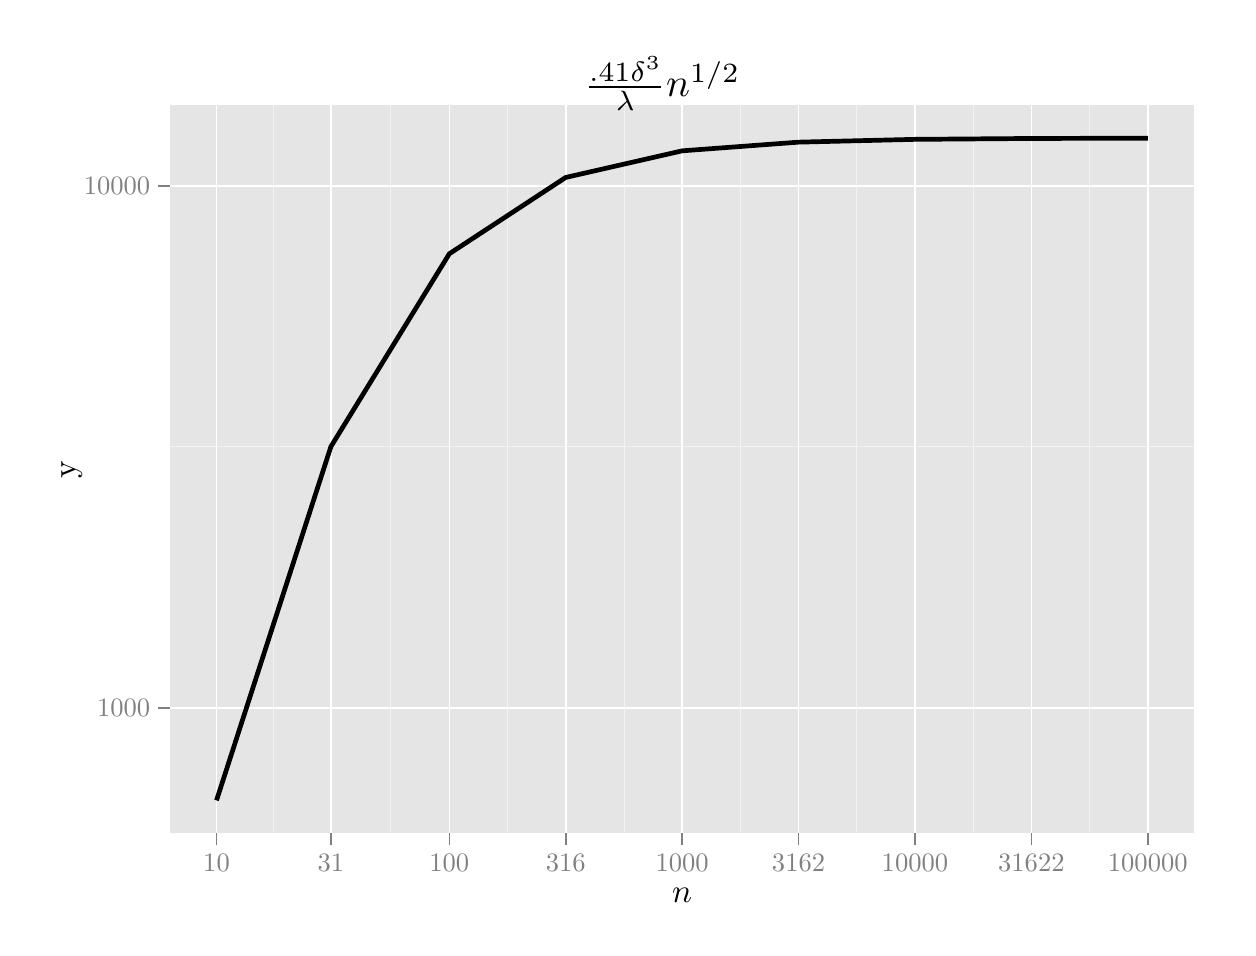
\begin{tikzpicture}[x=1pt,y=1pt]
\definecolor[named]{fillColor}{rgb}{1.00,1.00,1.00}
\path[use as bounding box,fill=fillColor,fill opacity=0.00] (0,0) rectangle (433.62,325.21);
\begin{scope}
\path[clip] (  0.00,  0.00) rectangle (433.62,325.21);
\definecolor[named]{drawColor}{rgb}{1.00,1.00,1.00}
\definecolor[named]{fillColor}{rgb}{1.00,1.00,1.00}

\path[draw=drawColor,line width= 0.6pt,line join=round,line cap=round,fill=fillColor] (  0.00,  0.00) rectangle (433.62,325.21);
\end{scope}
\begin{scope}
\path[clip] ( 51.42, 34.03) rectangle (421.57,297.23);
\definecolor[named]{fillColor}{rgb}{0.90,0.90,0.90}

\path[fill=fillColor] ( 51.42, 34.03) rectangle (421.57,297.23);
\definecolor[named]{drawColor}{rgb}{0.95,0.95,0.95}

\path[draw=drawColor,line width= 0.3pt,line join=round] ( 51.42,173.77) --
	(421.57,173.77);

\path[draw=drawColor,line width= 0.3pt,line join=round] ( 88.91, 34.03) --
	( 88.91,297.23);

\path[draw=drawColor,line width= 0.3pt,line join=round] (130.97, 34.03) --
	(130.97,297.23);

\path[draw=drawColor,line width= 0.3pt,line join=round] (173.39, 34.03) --
	(173.39,297.23);

\path[draw=drawColor,line width= 0.3pt,line join=round] (215.45, 34.03) --
	(215.45,297.23);

\path[draw=drawColor,line width= 0.3pt,line join=round] (257.53, 34.03) --
	(257.53,297.23);

\path[draw=drawColor,line width= 0.3pt,line join=round] (299.59, 34.03) --
	(299.59,297.23);

\path[draw=drawColor,line width= 0.3pt,line join=round] (341.65, 34.03) --
	(341.65,297.23);

\path[draw=drawColor,line width= 0.3pt,line join=round] (383.72, 34.03) --
	(383.72,297.23);
\definecolor[named]{drawColor}{rgb}{1.00,1.00,1.00}

\path[draw=drawColor,line width= 0.6pt,line join=round] ( 51.42, 79.46) --
	(421.57, 79.46);

\path[draw=drawColor,line width= 0.6pt,line join=round] ( 51.42,268.08) --
	(421.57,268.08);

\path[draw=drawColor,line width= 0.6pt,line join=round] ( 68.24, 34.03) --
	( 68.24,297.23);

\path[draw=drawColor,line width= 0.6pt,line join=round] (109.58, 34.03) --
	(109.58,297.23);

\path[draw=drawColor,line width= 0.6pt,line join=round] (152.37, 34.03) --
	(152.37,297.23);

\path[draw=drawColor,line width= 0.6pt,line join=round] (194.41, 34.03) --
	(194.41,297.23);

\path[draw=drawColor,line width= 0.6pt,line join=round] (236.50, 34.03) --
	(236.50,297.23);

\path[draw=drawColor,line width= 0.6pt,line join=round] (278.56, 34.03) --
	(278.56,297.23);

\path[draw=drawColor,line width= 0.6pt,line join=round] (320.62, 34.03) --
	(320.62,297.23);

\path[draw=drawColor,line width= 0.6pt,line join=round] (362.69, 34.03) --
	(362.69,297.23);

\path[draw=drawColor,line width= 0.6pt,line join=round] (404.75, 34.03) --
	(404.75,297.23);
\definecolor[named]{drawColor}{rgb}{0.00,0.00,0.00}

\path[draw=drawColor,line width= 1.7pt,line join=round] ( 68.24, 46.00) --
	(109.58,173.84) --
	(152.37,243.51) --
	(194.41,271.08) --
	(236.50,280.70) --
	(278.56,283.84) --
	(320.62,284.85) --
	(362.69,285.17) --
	(404.75,285.27);
\end{scope}
\begin{scope}
\path[clip] (  0.00,  0.00) rectangle (433.62,325.21);
\definecolor[named]{drawColor}{rgb}{0.50,0.50,0.50}

\node[text=drawColor,anchor=base east,inner sep=0pt, outer sep=0pt, scale=  0.96] at ( 44.30, 76.15) {1000};

\node[text=drawColor,anchor=base east,inner sep=0pt, outer sep=0pt, scale=  0.96] at ( 44.30,264.78) {10000};
\end{scope}
\begin{scope}
\path[clip] (  0.00,  0.00) rectangle (433.62,325.21);
\definecolor[named]{drawColor}{rgb}{0.50,0.50,0.50}

\path[draw=drawColor,line width= 0.6pt,line join=round] ( 47.15, 79.46) --
	( 51.42, 79.46);

\path[draw=drawColor,line width= 0.6pt,line join=round] ( 47.15,268.08) --
	( 51.42,268.08);
\end{scope}
\begin{scope}
\path[clip] (  0.00,  0.00) rectangle (433.62,325.21);
\definecolor[named]{drawColor}{rgb}{0.50,0.50,0.50}

\path[draw=drawColor,line width= 0.6pt,line join=round] ( 68.24, 29.77) --
	( 68.24, 34.03);

\path[draw=drawColor,line width= 0.6pt,line join=round] (109.58, 29.77) --
	(109.58, 34.03);

\path[draw=drawColor,line width= 0.6pt,line join=round] (152.37, 29.77) --
	(152.37, 34.03);

\path[draw=drawColor,line width= 0.6pt,line join=round] (194.41, 29.77) --
	(194.41, 34.03);

\path[draw=drawColor,line width= 0.6pt,line join=round] (236.50, 29.77) --
	(236.50, 34.03);

\path[draw=drawColor,line width= 0.6pt,line join=round] (278.56, 29.77) --
	(278.56, 34.03);

\path[draw=drawColor,line width= 0.6pt,line join=round] (320.62, 29.77) --
	(320.62, 34.03);

\path[draw=drawColor,line width= 0.6pt,line join=round] (362.69, 29.77) --
	(362.69, 34.03);

\path[draw=drawColor,line width= 0.6pt,line join=round] (404.75, 29.77) --
	(404.75, 34.03);
\end{scope}
\begin{scope}
\path[clip] (  0.00,  0.00) rectangle (433.62,325.21);
\definecolor[named]{drawColor}{rgb}{0.50,0.50,0.50}

\node[text=drawColor,anchor=base,inner sep=0pt, outer sep=0pt, scale=  0.96] at ( 68.24, 20.31) {10};

\node[text=drawColor,anchor=base,inner sep=0pt, outer sep=0pt, scale=  0.96] at (109.58, 20.31) {31};

\node[text=drawColor,anchor=base,inner sep=0pt, outer sep=0pt, scale=  0.96] at (152.37, 20.31) {100};

\node[text=drawColor,anchor=base,inner sep=0pt, outer sep=0pt, scale=  0.96] at (194.41, 20.31) {316};

\node[text=drawColor,anchor=base,inner sep=0pt, outer sep=0pt, scale=  0.96] at (236.50, 20.31) {1000};

\node[text=drawColor,anchor=base,inner sep=0pt, outer sep=0pt, scale=  0.96] at (278.56, 20.31) {3162};

\node[text=drawColor,anchor=base,inner sep=0pt, outer sep=0pt, scale=  0.96] at (320.62, 20.31) {10000};

\node[text=drawColor,anchor=base,inner sep=0pt, outer sep=0pt, scale=  0.96] at (362.69, 20.31) {31622};

\node[text=drawColor,anchor=base,inner sep=0pt, outer sep=0pt, scale=  0.96] at (404.75, 20.31) {100000};
\end{scope}
\begin{scope}
\path[clip] (  0.00,  0.00) rectangle (433.62,325.21);
\definecolor[named]{drawColor}{rgb}{0.00,0.00,0.00}

\node[text=drawColor,anchor=base,inner sep=0pt, outer sep=0pt, scale=  1.20] at (236.50,  9.03) {$n$};
\end{scope}
\begin{scope}
\path[clip] (  0.00,  0.00) rectangle (433.62,325.21);
\definecolor[named]{drawColor}{rgb}{0.00,0.00,0.00}

\node[text=drawColor,rotate= 90.00,anchor=base,inner sep=0pt, outer sep=0pt, scale=  1.20] at ( 17.30,165.63) {y};
\end{scope}
\begin{scope}
\path[clip] (  0.00,  0.00) rectangle (433.62,325.21);
\definecolor[named]{drawColor}{rgb}{0.00,0.00,0.00}

\node[text=drawColor,anchor=base,inner sep=0pt, outer sep=0pt, scale=  1.44] at (236.50,300.24) {$\frac{.41\delta^3}{\lambda}n^{1/2}\quad $};
\end{scope}
\end{tikzpicture}

    }
  \end{center}
\end{frame}

\begin{frame}{Conclusion}
  \begin{itemize}
  \item Friedman's test for non-vectorial and heterogeneous data. \pause
  \item MKL power competitive with best-performing kernel. \pause
  \item MKL can learn structure of data. \pause
  \item Normal-like null distributions. \pause
  \item Berry--Esseen-type convergence result via Stein's method of exchangeable pairs.
  \end{itemize}
\end{frame}

% \begin{frame}[allowframebreaks]{References}
%   \bibliographystyle{ieeetr}
%   \bibliography{ncray}
% \end{frame}

\end{document}
